% Format teze zasnovan je na paketu memoir
% http://tug.ctan.org/macros/latex/contrib/memoir/memman.pdf ili
% http://texdoc.net/texmf-dist/doc/latex/memoir/memman.pdf
% Podešava se veličina papira, veličina slova i jednostrano štampanje
% Ne menjati ove parametre
\documentclass[a4paper,12pt,oneside]{memoir}

% Paket koji definiše sve specifičnosti doktorata Matematičkog fakulteta
\usepackage{matfdoktorat}
\usepackage{presek_reci}


% Datoteka sa literaturom u BibTex tj. BibLaTeX/Biber formatu
\bib{danijela_doktorat}

% Ime doktoranda na srpskom jeziku (u odabranom pismu)
\autor{Данијела Симић}
% Ime doktoranda na engleskom jeziku
\author{Danijela Simic}
% Naslov teze na srpskom jeziku (u odabranom pismu)
\naslov{Формализација различитих модела геометрије и примене у верификацији аутоматских доказивача теорема}
% Naslov teze na engleskom jeziku
\title{Formalization of various geometry models and applications in verification of automated theorem provers}
% Godina u kojoj je teza predana komisiji
\godina{2017}
% Ime i afilijacija mentora (u odabranom pismu)
\mentor{др Филип \textsc{Марић}, ванредни професор\\ Универзитет у Београду, Математички факултет}
% Ime i afilijacija prvog člana komisije (u odabranom pismu)
\komisijaA{др Предраг \textsc{Јаничић}, редовни професор\\ Универзитет у Београду, Математички факултет}
% Ime i afilijacija drugog člana komisije (u odabranom pismu)
\komisijaB{др Срђан \textsc{Вукмировић}, ванредни професор\\ Универзитет у Београду, Математички факултет}
% Ime i afilijacija trećeg člana komisije (opciono)
\komisijaC{др Петар \textsc{Максимовић}, Research Fellow \\ Imperial College London \\ Научни сарадник, Математички институт САНУ}
% Ime i afilijacija četvrtog člana komisije (opciono)
% \komisijaD{}
% Datum odbrane (obrisati ili iskomentarisati narednu liniju ako datum odbrane nije poznat)
%\datumodbrane{15. јануар 2016.}

% Apstrakt na srpskom jeziku (u odabranom pismu)
\apstr{% 

У овој тези представљена је интерактивна формализација модела разних
геометрија и алгебарских метода аутоматског доказивања геометријских
теорема.
 
Представљен је наш рад на формализацији аналитичке (Декартове)
планарне геометрије у оквиру асистента за доказивање теорема
\emph{Isabelle/HOL}. Дајемо неколико еквивалентних дефиниција
Декартове координатне равни и доказујемо да је она модел синтетичких
планарних геометрија (коришћењем аксиоматског система Тарског и
аксиоматског система Хилберта). Такође, дискутујемо о неколико техника
којима се поједностављују и аутоматизују докази. Како је један од
наших циљева да подржимо коришћење асистената за доказивање теорема у
математичком образовању, наше излагањe ће бити блиско стандардним
дефиницијама у уџбеницима, али потпуно формално и машински
провериво. Ова формализација представља део потребне инфраструктуре за
имплементацију процедура одлучивања базираних на аналитичкој
геометрији у оквиру асистената за доказивање теорема.

Додатно, формално разматрамо и геометрију комплексне равни. Блиска
повезаност између комплексних бројева и геометрије је добро позната и
пажљиво је изучавана још вековима уназад. Основни објекти који су
изучавани су комплексна раван (обично проширена једном бесконачном
тачком), њени објекти (тачке, праве и кругови), и група трансформација
која на њих делује (на пример, инверзије и Мебијусове
трансформације). У овој тези, ми формално посматрамо геометрију
комплексних бројева и представљамо потпуно механички верификовану
теорију у оквиру асистента за доказивање теорема
\emph{Isabelle/HOL}. Дискутујемо о различитим приступима формализацији
и главним предностима приступа који је више алгебарски
оријентисан. Поред примена у формализацији математике и у образовању,
овај рад је основа за формалну анализу нееуклидских геометрија и
њихове међусобне повезаности. Такође, представљамо и формализацију
дела аксиоматског система Тарског у оквиру Поенкареовог диск модела у
систему \emph{Isabelle/HOL}.

Треће, анализирамо везу између геометрије и полинома, као и примене
која ова веза даје. У еуклидској геометрији објекти и релације међу
њима могу се изразити полиномијалним једнакостима. Додатно, било која
геометријска конструкција може се изразити скупом полиномијалних
једнакости, а геометријска тврђења се могу доказати коришћењем
алгебарских метода (на пример, метод Гребнерових база или Вуовом
методом) над скупом полинома. Дајемо опис алгоритма у систему
\emph{Isabelle/HOL} који као улазни податак прихвата геометријску
конструкцију записану коришћењем термова, а враћа одговарајући скуп
полинома. Наш даљи рад ће бити примена методе Гребнерових база у
оквиру система \emph{Isabelle/HOL} над генерисаним полиномима у намери
да се докаже исправност дате конструкције. Додатно, истражујемо како
се конструкције у тродимензионалном простору могу приказати коришћењем
полинома. Истражујемо два различита приступа у извођењу ових полинома
и онда поредимо ефикасност алгебарских метода у зависности од
коришћеног приступа. Представљамо потпуно аутоматски систем за
превођење геометријских конструкција из стереометрије у скуп
полинома. Наш даљи рад ће бити да повежемо представљени систем са
динамичким геометријским софтвером и на тај начин да омогућимо
студентима лакше коришћење овог аутоматизованог система за доказивање
у стереометрији.}

% искоментарисати енглески
% Apstrakt na engleskom jeziku
\abstr{

In this thesis is presented interactive formalization of various
models of geometry and algebraic methods for automated proving
geometry theorems.

We present our current work on formalizing analytic (Cartesian) plane
geometries within the proof assistant Isabelle/HOL. We give several
equivalent definitions of the Cartesian plane and show that it models
synthetic plane geometries (using both Tarski's and Hilbert's axiom
systems). We also discuss several techniques used to simplify and
automate the proofs. As one of our aims is to advocate the use of
proof assistants in mathematical education, our exposure tries to
remain simple and close to standard textbook definitions, but
completely formal and mechanically verifiable. This formalization
presents the develop of the necessary infrastructure for implementing
decision procedures based on analytic geometry within proof
assistants.


Furthermore, we investigate complex numbers. Deep connections between
complex numbers and geometry had been well known and carefully studied
centuries ago. Fundamental objects that are investigated are the
complex plane (usually extended by a single infinite point), its
objects (points, lines and circles), and groups of transformations
that act on them (e.g., inversions and M\"obius transformations). In
this thesis we treat the geometry of complex numbers formally and
present a fully mechanically verified development within the theorem
prover Isabelle/HOL. We discuss different approaches to formalization
and discuss major advantages of the more algebraically oriented
approach. Apart from applications in formalizing mathematics and in
education, this work serves as a ground for formally investigating
various non-Euclidean geometries and their intimate connections. We
also present a formalization of part of Tarski axiom system withing
Poincare disk model in Isabelle/HOL.

Further on, we analyze connections between geometry and polynomials
and the use of these connections. In Euclidean geometry, objects and
relations between them can be expressed as polynomials.  Further, any
geometry construction can be expressed by set of polynomials and
geometry statements can be proved by using algebraic methods (e.g. the
Gr\"obner bases method or Wu's method) over that set of
polynomials. We describe an implementation of an algorithm in
Isabelle/HOL that accepts a term representation of a geometry
construction and returns its corresponding set of polynomials. Our
further work will be to use the method of Gr\"obner bases within the
Isabelle system on the generated polynomials, in order to prove
correctness of the given construction.  Furthermore, we investigate
how spatial geometry constructions can be presented using
polynomials. We investigate two different approaches in deriving those
polynomials and then compare efficiency of algebraic provers depending
on the approach used. We present a fully automated system for
transforming geometry constructions into set of polynomials. Our
further work would be to relate these geometry provers with dynamic
geometry software and thus make easier for students to use it.  }

% Ključne reči na srpskom jeziku (u odabranom pismu)
\kljucnereci{асистент за доказивање теорема, геометрија, интерактивно
  доказивање у геометрији, аутоматско доказивање у геометрији,
  хиперболичка геометрија, стереометрија, аксиоматски систем Тарског,
  аксиоматски систем Хилберта, Декартов координатни систем}

% Ključne reči na engleskom jeziku
\keywords{proof assistants, geometry, interactive proving in geometry,
  automated proving in geometry, hyperbolic geometry, spatial geometry,
  Tarski axiom system, Hilbert axiom system, Cartesian coordinate
  system}

% Šira i uža oblast teze na srpskom jeziku (u odabranom pismu)
\oblast{рачунарство}
\uzaoblast{аутоматско резоновање}

% Šira i uža oblast teze na engleskom jeziku
\area{computer science}
\subarea{automated reasoning}

% Univerzalna decimalna klasifikacija (UDK tj. UDC)
% https://en.wikipedia.org/wiki/Universal_Decimal_Classification
\udk{004.832.3:514(043.3)}

%!!!!!!!!!!!!!!!!!!!!!!!!!!!!!!!!!!!! ukljucujem sta meni treba
\usepackage{moji_paketi}

\begin{document}
% ==============================================================================
% Uvodni deo teze
\frontmatter
% ==============================================================================
% Naslovna strana
\naslovna
% Naslovna strana na engleskom jeziku
\naslovnaen
% Strana sa podacima o mentoru i članovima komisije
\komisija
% Strana sa posvetom (u odabranom pismu)
\posveta{родитељима, Милијани и Драгану Петровићу}

\newpage

\begin{Huge}
\emph{Захвалница}
\end{Huge}

\bigskip
\bigskip


Велику захвалност дугујем свом ментору, професору Филипу
Марићу. Професоров велики ентузијазам, знање и безрезервна подршка су
ми много помогли у току докторских студија и приликом рада на
различитим истраживањима и пројектима. Он ме је упутио у диван свет
интерактивног доказивања теорема и бројним саветима и сугестијама ме
је мотивисао да што више научим и напредујем. Посебно истичем његове
иновативне идеје и позитивност која је често утицала да са еланом и
новом енергијом наставим да се бавим проблемима на које сам у раду
наишла. Захваљујући њему сам објавила радове у часописима и
конференцијама и завршила ову тезу, a без његове помоћи и подршке тога
не би било.

Захваљујем се и професору Предрагу Јаничићу, он ме је упутио у свет
геометрије и аутоматског доказивања у геометрији. Многим саветима и
сугестијама је утицао да финална верзија тезе буде квалитетнија и
потпунија. Захваљујући њему упознала сам и многе истраживаче из других
земаља и тако ми је створена могућност да размењујем искуства и да
учествујем у пројектима и ван граница наше земље. Напоменула бих и да
са професором сарађујем у настави и да је вишегодишње заједничко
држање курсева било једно лепо и пријатно искуство.

Захваљујем се и професорима Срђану Вукмировићу и Петру Максимовићу на
пажљивом читању тезе. Њихови коментари су значајно унапредили текст
тезе, али су дали и нови поглед на проблеме којима се бавим и пружили
су ми нове идеје како да истраживање наставим.

Захваљујем се и свим члановима катедре, професорима и асистентима. Сви
су били заиста дивни сарадници и од првих дана рада ми значајно
помогли да напредујем као наставник и као истраживач. Дали су ми
бројне савете, одменили када је било потребно или улепшали дан на
послу. Могу рећи да сам заиста срећна што радим у тако динамичном,
позитивном и колегијалном колективу.

Посебну захвалност дугујем својим родитељима којима ову тезу
посвећујем. Они су ми били ослонац и подршка током целог
живота. Захваљујући њиховој неизмерној љубави и упорности сам
остварила многе циљеве на пословном и приватном плану. Од првог дана
школовања су веровали у мене и бодрили ме, помагали и упућивали да
увек тежим да више научим, сазнам и постигнем.

Коначно, захваљујем се и свом супругу Михаилу. Био је велика подршка у
раду на овој тези, одмењивао ме у разним пословима, подизао дух када
бих посустала, више пута заједно са мном читао тезу и увек веровао да
ћу успети. Његова љубав и позитивна енергија су ми учинили рад на тези
лакшим и лепшим.
\newpage


% Strana sa podacima o disertaciji na srpskom jeziku
\apstrakt
% Strana sa podacima o disertaciji na engleskom jeziku
\apstrakten
% Sadržaj teze
\tableofcontents*

% ==============================================================================
% Glavni deo teze
\mainmatter
% ==============================================================================

%\chapter{Превод ADG-а}

% ------------------------------------------------------------------------------
\section{Увод}
% ------------------------------------------------------------------------------
У класичној математици постоји много различитих геометрија. Такође,
различита су и гледишта шта се сматра стандардном (Еуклидском)
геометријом. Понекад, геометрија се дефинише као независна формална
теорија, а понекад као специфични модел. Наравно, везе између
различтих заснивања геометрије су јаке. На пример, може се показати да
Декартова раван представља модел формалних теорија геометрије.

Традиционална Еукидска (синетичка) геометрија, која датира још од
античке Грчке, је геометрија заснована на често малом скупу основних
појмова (на пример, тачке, линије, релација подударности, \ldots) и на
скупу аксиома које имплицитно дефинишу ове основне појмове.  Постоји
више варијанти аксиоматског система за Еуклидску геометрију, а
најважнији су Еуклидски систем аксиома (из његовог рада "Елементи"),
потом Хилбертов систем аксиома\cite{hilbert}, систем аксиома
Тарског\cite{tarski} и најмодернија варијанта -- Авигадов систем
аксиома\cite{avigad}.

Једна од најзначајнијих открића у математици, које датира из XVII
века, јесте Декартово откриће координатног система и оно је омогућило
да се алгебарским изразима представе геометријски облици. То је довело
до рада на новој математичкој области која се зове \emph{аналитичка
  геометрија}. Она је послужила да споји геометрију и алгебру и била
је веома важна за откриће бесконачности и математичке анализе.

Последњих година, са појавом модерних интерактвних доказивача теорема,
многе класичне математичке теорије су формално механички
анализиране. Међу њима је и геометрија и постоји неколико покушаја да
се формализују раличите геометрије и различити приступи у
геометрији. Ми нисмо упознати да је поптпуно комплетно формализован
Хилбертов систем\cite{hilbert} или систем аксиома
Тарског\cite{tarski}, али значајно кораци су направљени и велики
делови ових теорија су формализоване у оквиру интерактивних доказивача
теорема\cite{hilbert-isabelle,narboux,projective-coq1}.  Како искуство
за сада показује, коришћењем доказивача теорема значајно се повећава
ниво прецизности јер се показало да су многе класичне математичке
књиге непрецизне, а понекад чак имају и грешке. Зато би приликом
формалног заснивања геометрије требало користити доказивач теорема, а
у нашем раду ми смо користили Isabelle/HOL\cite{Isabelle} доказивач.

Главна примена нашег рада је у аутоматском доказивању теорема у
геометрији и у математичком образовању и учењу геометрије.

Код аутоматског доказивања теорема у геометрији, аналитички приступ у
доказима се показао далеко супериорнији у односу на остале
доказиваче. Најуспешнији методи на овом пољу су \emph{алгебарски
  методи} (Вуоов метод\cite{wu} и метод Гребнерових
база\cite{buchberger,kapur}) и они се заснивају на репрезентацији
тачака коришћењем координата. Модерни доказивачи теорема који се
заснивају на овим методима су коришћени да се докажу стотине
нетривијалних теорема. Са друге стране, доказивачи теорема засновани
на синтетичкој аксиоматизацији нису толико успешни. Већина система са
аналитичким приступом за доказивање теорема се користи као софтвер
којем се верује иако нису повезани са модерним интерактивним
доказивачима теорема. Да би се повећала њихова поузданост потребно их
је повезати са модерним интерактивним доказивачима теорема и то је
могуће учинити на два начина -- њиховом имплементацијом у оквиру
интерактивног доказивача теорема и показивањем њихиове исправности или
коришћењем интерактивних доказивача да провере њихова
тврђења. Неколико корака у овом правцу је већ
направљено\cite{wucoq,thedu}.

У математичком образовању у средњим школама и на факултетима оба
приступа у геометрији (аналитички и синтетички) се
демонстрирају. Ипак, док се синтетички приступ предаје као ригорозан
систем (са намером да се демонстрира ригорозан аксиоматски приступ),
аналитичка геометрија се показује много мање формално (понекад само
као део рачуна calculus).  Такође, ова два приступа се показују
независно, и веза између ова два приступа се ретко формално показује у
оквиру стандарог наставног плана.

Имајћи све ово на уму, ова рад покушава да премости више празнина за
које мислимо да тренутно постоје у формализацији геометрије.


\begin{enumerate}
\item Прво, наш циљ је да формализујемо Декартову геометрију у оквиру
      интерактивног доказивача теорема, са ригорозним приступом, али веома блиско
      стандарном средњошколском образовању.
\item Намеравамо да покажемо да су разиличите дефиниције основних појмова
      аналитичке геометрије које можемо видети у литератури заправо еквивалентне,
      и да заправо представљају јединствен апстрактни ентитет -- Декартову раван.
\item Намеравамо да покажемо да стандарна геометрија координатне равни
      представља модел неколико геометријских аксиоматизација (пре свега
      систем аксиома Тарског и Хилбертов систем аксиома).
\item Желимо формално да анализирамо теоретске особине различитих аксиоматских система
      (на пример, желимо да покажемо да сви модели Хилбертовог система аксиома су
      изоморфни стандарној координатној геометрији).
\item Желимо формално да анализирамо аксиоматизације и моделе не-Еуклидске геометрије
      и њихове особине (на пример, да покажемо да је Поинкареов диск модел запараво модел
      геометрије Лобачевског).
\item Желимо да формално успоставимо везу између геометрије координатног система са
      алгебарским методама за аутоматско доказивање теорема у геометрији.
\end{enumerate}



Поред тога што су многе теореме формализоване и доказане у оквиру
система Isabelle/HOL, ми такође дискутујемо и наше искуство у примени
различитих техника за поједностављење доказа.  Најзначајнија техника
је "без губитка на општости" (``wlog''), која прати приступ
Харисона\cite{wlog} и која је оправдна коришћењем разних
изометријиских трансформација.

% ------------------------------------------------------------------------------
\section{Основни појмови}
\label{sec:background}
% ------------------------------------------------------------------------------
\paragraph{ Isabelle/HOL.}  Isabelle/HOL је интерактивни
доказивач теорема који је заснова на логици вишег реда (HOL).  Он
обезбеђује моћне аутоматске методе за доказивање, који су обично
засновани на симлификацији класичном резоновању. Isar је декларативни
језик за доказе у Isabell/HOL систему, који дозвољава писање
структурних, читљивих доказа. У Isabelle/HOL систему $\llbracket P_1;
\ldots P_n \rrbracket \Longrightarrow Q$ значи ако $P_1$, \ldots,
$P_n$ је тачно, онда $Q$ је такође тачно. Ова нотација се користи да
означи и правила закључивања и тврђења (леме, теореме).  Језик Isar
такође омогоћува и нотацију {\em assumes "$P_1$" \ldots "$P_n$"\ shows
  "$Q$"\ }, и она ће бити коришћена у овом раду. Такође, користићемо и
везнике међу објектима $\wedge$, $\vee$, $\longrightarrow$, и
$\longleftrightarrow$ за означавање коњукције, дисјункције, имликације
и логичке еквиваленције. Квантификатори ће бити означени са $\forall
x.\ P x$ и $\exists x.\ P x$.

% ------------------------------------------------------------------------------
\section{Формализација геометрије Декартове равни}
\label{sec:cartesian}
% ------------------------------------------------------------------------------

Када се формализује теорија, мора се одлучити који појмови ће бити
основни, а који појмови ће бити дефинисани помоћу тих основних
појмова. Циљ наше формализације аналитичке геометрије је да успостави
везу са синтетичком геометријом, па зато има исте основне појмове који
су дати у синтетичком приступу. Свака геометрија има класу објеката
који се називају \emph{тачке}. Неке геометрије (на пример, Хилбертова)
има и додатни скуп објеката који се наизвају \emph{линије}, док неке
геометрије (на пример, геометрија Тарског) уопште не разматра линије .
У неким геометријама, линије су дефинисани појам, и оне су дефинисане
као скуп тачака.  Ово подразумева рад са теоријом скупова, а многе
аксиоматизације желе то да избегну.  У нашој формализацији аналитичке
геометрије, ми ћемо дефинисати и тачке и линије јер желимо да
омогућимо анализу и геометрије Тарског и геометрије Хилберта. Основна
релација која спаја тачке и линије је релације \emph{инциденције},
која неформално означава да линија садржи тачку (или дуално да се
тачка налази на линији). Други примитивни појмови (у већини
аксиоматских система) су релација \emph{између} (која дефише редослед
колинеарних тачака) и релација \emph{конгруенције}.

Важно је напоменути да су обично многи појмови који су заправно
изведени појмови у синтетичкој геометрији у аналитичком геометрији
дати у облику дефиниција. На пример, у књигама за средњу школу дефише
се да су линије нормалне ако је производ њихових праваца $-1$. Ипка,
ово нарушава везу са синтетичком геометријом (где је нормалност
изведени појам) јер би оваква карактеризација требало да буде доказана
као теорема, а не узета као дефиниција.

\subsection{Тачке у аналитичкој геометрији.}
Тачка у реалној координатној равни је одређена са својим $x$ и $y$
координатама. Зато, тачке су парови реалних бројева ($\mathbb{R}^2$),
што се може лако формализовати у Isabelle/HOL систему са {\tt
  type\_synonym\ $point^{ag}\ =\ "real \times real"$}.

\subsection{Редослед тачака.} Редослед (колинерних) тачака се
дефинише коришћењем релације \emph{између}. Ово је релација која има
три аргумента, $\mathcal{B}(A, B, C)$ означава да су тачке $A$, $B$, и
$C$ колинеране и да је тачка $B$ између тачака $A$ и $C$. Ипак, неке
аксиоматизације (на пример, аксиоматизација Тарског) дозвољава случај
када је тачка $B$ једнака тачки $A$ или тачки $C$ (рећи ћемо да је
релација између инклузивна, док неке друге аксиоматизације (на пример,
Хилбертова аксиоматизација) не дозвољавају једнакост тачака (и тада
кажемо да је релација између ексклузивна. У првом случају, тачке $A$,
$B$ и $C$ задовољавају релацију између ако постоји реалан број $0 \le
k \le 1$ такав да $\vect{AB} = k \cdot \vect{AC}$. Желимо да
избегенемо експлицитно коришћење вектора јер су они чешће изведени, а
ређе примитиван појам у синтетичкој геометрији, тако да релацију
између формализујемо у Isabelle/HOL систему на следећи начин:

{\tt
\begin{tabbing}
\hspace{5mm}\=\hspace{5mm}\=\kill
$\agbett{(xa, ya)}{(xb, yb)}{(xc, yc)} \longleftrightarrow$\\
\>$(\exists (k::real).\ 0 \le k \ \wedge\ k \le 1 \ \wedge$\\
\>\>$(xb - xa) = k \cdot (xc - xa) \ \wedge\ (yb - ya) = k \cdot (yc - ya))$
\end{tabbing}
}

\noindent Ако захтевамо да тачке $A$, $B$ и $C$ буду различите, она
мора да важи $0 < k < 1$, и релацију ћемо означавати са
$\agbeth{}{}{}$.

\subsection{Конгруенција.} Релација конгрунеције дефинише се на паровима
тачака. Неформално, $\congrt{A}{B}{C}{D}$ означава да је сегмент $AB$
конгруентан сегменту $CD$. Стандардна метрика у $\mathbb{R}^2$
дефинише да растојање међу тачкама $A(x_A, y_A)$, $B(x_B, y_B)$ је
$d(A, B) = \sqrt{(x_B-x_A)^2+(y_B-y_A)^2}$. Квадратно растојање се
дефинише као $\agsqdist{A}{B} = (x_B-x_A)^2+(y_B-y_A)^2$. Тачке $A$ и
$B$ су конгруентне тачкама $C$ и $D$ ако и само ако $\agsqdist{A}{B} =
\agsqdist{C}{D}$. У Isabelle/HOL систему ово се може формализовати на
следећи начин:

{\tt
\begin{tabbing}
$\agsqdist{(x_1, y_1)}{(x_2, y_2)} = (x_2-x_1)\cdot (x_2-x_1)+(y_2-y_1)\cdot (y_2-y_1)$\\
$\agcongr{A_1}{B_1}{A_2}{B_2} \longleftrightarrow \agsqdist{A_1}{B_1} = \agsqdist{A_2}{B_2}$
\end{tabbing}
}

\subsection{Права и инциденција.}

\paragraph{Једначина праве.}
Праве у Декартовој координатној равни се обично представљају
једначинама облика $Ax + By + C = 0$, па тако тројка $(A, B, C) \in
\mathbb{R}^3$ означава линију. Ипак, тројке у којима је $А = 0$ и $B =
0$ морају бити изузете јер не представљају исправну једначину
праве. Такође, једначине $Ax + By + C = 0$ и $kAx + kBy + kC = 0$, за
реално $k \neq 0$, означавају исту праву. Зато права не може бити
дефинисана коришћењем само једне једначине, већ права мора бити
дефинисана као класа једначина које имају пропорционалне
коефициенте. Формализација у систему Isabelle/HOL се састоји из
неколико корака. Прво, дефинише се домен валидних тројки који су
коефициенти једначине.
{\tt
\begin{tabbing}
typedef $\mathit{line\_coeffs}^{ag}$ = \\
\hspace{5mm}$\{((A::real), (B::real), (C::real)).\ A \neq 0 \vee B \neq 0\}$
\end{tabbing}
}
\noindent Када је овај тип дефинисан, функција
$\mathit{Rep\_line\_coeffs}$ конвертује апстрактне вредности овог типа
у њихове конкретне репрезентације (тројке реалних бројева), а функција
$\mathit{Abs\_line\_coeffs}$ конвертује (валидне) тројке у вредности
које припадају овом типу.

Две тројке су еквиваленте ако и само ако су пропорционалне.
{\tt
\begin{tabbing}
\hspace{5mm}\=\kill
$l_1 \approx^{ag} l_2$ $\longleftrightarrow$ \\
\>  $(\exists\ A_1\,B_1\,C_1\,A_2\,B_2\,C_2.$\\
\>  $(\mathit{Rep\_line\_coeffs}\ l_1 = (A_1, B_1, C_1)) \ \wedge\ \mathit{Rep\_line\_coeffs}\ l_2 = (A_2, B_2, C_2)\ \wedge$\\
\>  $(\exists k.\ k \neq 0 \,\wedge\, A_2 = k\cdot A_1 \,\wedge\,  B_2 = k\cdot B_1\,\wedge\,C_2 = k\cdot C_1))$
\end{tabbing}
}
\noindent Показано је да је ово релација еквиваленције. Дефиниција
типа праве користи подршку за количничке типове и количничке
дефиниције које су скоро интегрисане у систем Isabelle/HOL. Значи
права (тип $\mathit{line^{ag}}$) се дефинише коришћењем
\verb|quotient\_type| команде као класа еквиваленције над релацијом
$\approx^{ag}$.

Да би избегли коришћење теорије скупова, геометријске аксиоматизације
које експлицитно разматрају праве користе релацију инциденције. Ако се
користи претходна дефиниција за праву, онда проверавање инциденције се
своди на израчунавање да ли тачка $(x, y)$ задовољава једначину праве
$A\cdot x + B\cdot y + C = 0$, за неке коефицијенте $А$, $B$, и $C$
који су представници класе.
{\tt
\begin{tabbing}
\hspace{5mm}\=\hspace{5mm}\=\kill
$ag\_in\_h\ (x, y)\ l \longleftrightarrow$\\
\>$(\exists\ A\ B\ C.\ \mathit{Rep\_line\_coeffs}\ l = (A,\ B,\ C) \,\wedge\,  (A\cdot x + B\cdot y + C = 0))$
\end{tabbing}
}

Ипак, да би показали да је релација заснована на представницима класе
добро заснована, мора бити показано да ако се изаберу други
представници класе $А'$, $B'$, и $C'$ (који су пропорционални са $А$,
$B$, и $C$), онда $A'\cdot x + B'\cdot y + C = 0$. Зато, у нашој
Isabelle/HOL формализацији, ми користимо пакет који подржава рад са
количничким типовима (quotient package). Онда $\aginh{A}{l}$ се
дефинише коришћењем \verb|quotient\_definition| која се заснива на
релацији $ag\_in\_h$. Лема добре дефинисаности је
{\tt
\begin{tabbing}
\hspace{5mm}\=\hspace{5mm}\=\kill
lemma \\
\>shows "$l \approx l' \Longrightarrow ag\_in\_h\ P\ l = ag\_in\_h\ P\ l'$"
\end{tabbing}
}


\paragraph{Афина дефиниција.}
У афиној геометрији, права се дефинише помоћу фиксне тачке и
вектора. Као и тачке, вектори такође могу бити записани као пар
реалних бројева {\tt type\_synonym\ $vec^{ag}\ =\ "real \times
  real"$}. Вектори дефинисани на овај начин чине векторски простор (са
природно дефинисаним векторским збиром и скаларним производом). Тачке
и вектори се могу сабирати као $(x, y) + (v_x, v_y) = (x + v_x, y +
v_y)$. Зато, права се записује као тачка и вектор који је различит од
нуле: 
{\tt
\begin{tabbing}
typedef $\mathit{line\_point\_vec}^{ag} =\{(p::point^{ag}, v::vec^{ag}).\ v \neq (0, 0)\}$
\end{tabbing}
}

Ипак, тазличите тачке и вектори могу заправо одређивати једну те исту
праву, па конструкција са количничким типом опет мора бити коришћена.

{\tt
\begin{tabbing}
\hspace{5mm}\=\\
$l_1 \approx^{ag} l_2 \longleftrightarrow (\exists\,p_1\,v_1\,p_2\,v_2.$\\
\>$\mathit{Rep\_line\_point\_vec}\ l_1 = (p_1, v_1) \,\wedge\,  \mathit{Rep\_line\_point\_vec}\ l_2 = (p_2, v_2) \,\wedge$\\
\>$(\exists k m.\ v_1 = k\cdot v_2 \,\wedge\, p_2 = p_1 + m\cdot v_1))$
\end{tabbing}
}
\noindent Показује се да је ово заиста релација еквиваленције. Онда се
тип праве ($\mathit{line^{ag}}$) дефинише коришћењем команде
\verb|quotient\_type|, као класа еквиваленције над релацијом
$\approx^{ag}$.

У овом случају, инциденција се дефинише на начин који можете видети у
наставку (поново се уопштава lifted) коришћењем количничког пакета,
након што се покаже добра дефинисаност).

{\tt
\begin{tabbing}
\hspace{5mm}\=\hspace{5mm}\=\kill
$ag\_in\_h\,p\,l,\longleftrightarrow\,(\exists\,p_0\,v_0.\,\mathit{Rep\_line\_point\_vec}\,l = (p_0, v_0) \,\wedge\,  (\exists k.\,p = p_0 + k \cdot v_0))$
\end{tabbing}
}

Још једна могућа дефиниција праве је класа еквиваленције парова
различитих тачака. Ми нисмо формализовали овај приступ јер је
тривиално изоморфан са афином дефиницијом (разлика тачака је вектор
који се појављује у афиној дефиницији).

\subsection{Изометрије}

У синтетичкој геометрији изометрије се уводе коришћењем
дефиниције. Рефлексије могу прве да се дефинишу, а онда се друге
изометрије могу дефинисати као композиција рефлексија. Ипак, у нашој
формализацији , изометрије се користе само као помоћно средство да
упросте наше доказе (што ће бити додатно појашњено у одељку
\ref{sec:iso}). Зато ми нисмо били заинтересовани да дефинишемо
изометрије као примитивне појмове (као што су тачке и конгруенција)
него смо представили аналитичке дефиниције и доказали својства која су
потребна за касније доказе.

Транслација је дефинисана преко датог вектора (који није експлицитно
дефининсан, већ је представљен као пар реалних бројева). Формална
дефиниција у Isabelle/HOL је једноставна.

{\tt
\begin{tabbing}
$\agtransp{(v_1, v_2)}{(x_1, x_2)} = (v_1 + x_1, v_2 + x_2)$
\end{tabbing}
}

Ротација је параметризована за реални параметар $\alpha$ (који
представља угао ротације), а ми само посматрамо ротације око
координатног почетка (остале ротације могу се добити као композиција
транслације и ротације око координатног почетка).  Користимо основна
правила тригонометрије да би добили следећу формалну дефиницију у
систему Isabelle/HOL.

{\tt
\begin{tabbing}
$\agrotp{\alpha}{(x, y)} = ((\cos \alpha)\cdot x - (\sin
\alpha)\cdot y , (\sin \alpha)\cdot x + (\cos \alpha)\cdot y)$
\end{tabbing}
}

Такође, централна симетрија се лако дефинише коришћењем координата
тачаке:
 {\tt
\begin{tabbing}
$\agsymp{(x, y)} = (-x, -y)$
\end{tabbing}
}

Важна особина свих изометрија је својство инваријантности, тј.  оне
чувају основне релације (као што су између и конгруенција).

{\tt
\begin{tabbing}
\hspace{5mm}\=\kill
$ \agbett{A}{B}{C} \longleftrightarrow \agbett{(\agtransp{v}{A})}{(\agtransp{v}{B})}{(\agtransp{v}{C})}$\\
$\agcongr{A}{B}{C}{D} \longleftrightarrow$\\
\> $\agcongr{(\agtransp{v}{A})}{(\agtransp{v}{B})}{(\agtransp{v}{C})}{(\agtransp{v}{D})}$\\
$\agbett{A}{B}{C} \longleftrightarrow \agbett{(\agrotp{\alpha}{A})}{(\agrotp{\alpha}{B})}{(\agrotp{\alpha}{C})}$\\
$\agcongr{A}{B}{C}{D} \longleftrightarrow
   \agcongr{(\agrotp{\alpha}{A})}{(\agrotp{\alpha}{B})}{(\agrotp{\alpha}{C})}{(\agrotp{\alpha}{D})}$\\
$\agbett{A}{B}{C} \longleftrightarrow \agbett{(\agsymp{A})}{(\agsymp{B})}{(\agsymp{C})}$\\
$\agcongr{A}{B}{C}{D} \longleftrightarrow
   \agcongr{(\agsymp{A})}{(\agsymp{B})}{(\agsymp{C})}{(\agsymp{D})}$
\end{tabbing}
}

Изометрије се пре свега користе да трансформишу тачку у њену канонску
позицију (обично померањем на $y$-осу).  Следеће леме показује да је
то могуће учинити.

{\tt
\begin{tabbing}
$\exists v.\ \agtransp{v}{P} = (0, 0)$\\
$\exists \alpha.\ \agrotp{\alpha}{P} = (0, p)$\\
$\agbett{(0, 0)}{P_1}{P_2} \longrightarrow \exists \alpha\ p_1\
p_2.\ \agrotp{\alpha}{P_1} = (0, p_1) \wedge \agrotp{\alpha}{P_2}
= (0, p_2)$
\end{tabbing}
}

Изометријске трансформације линија се дефинишу коришћењем
изометријских трансформација над тачкама (линија се трансформише тако
што се трансформишу две њене произвољне тачке.

%------------------------------------------------------------------------------
\section{Коришћење изометријских трансформација}
\label{sec:iso}
% ------------------------------------------------------------------------------
Једна од најважнијих техника која је коришћења за упрошћавање
формализације ослањала се на коришћење изометријских
трансформација. Ми ћемо покушати да представимо мотивациони разлог за
примену изометрија на следећем, једноставном примеру.

Циљ је да покажемо да у нашем моделу, ако $\agbett{A}{X}{B}$ и
$\agbett{A}{B}{Y}$ онда важи $\agbett{X}{B}{Y}$. Чак и на овом
једноставном примеру, ако применимо директан доказ, без коришћења
изометријских трансформација, алгебарски рачун постаје превише
комплексан.

Нека важи $A=(x_A, y_A)$, $B=(x_B, y_B)$, и $X=(x_X, y_X)$.  Како
$\agbett{A}{X}{B}$ важи, постоји реалан број $k_1$, $0 \le k_1 \le 1$,
такав да $(x_X - x_A) = k_1 \cdot (x_B - x_A)$, и $(y_X - y_A) = k_1
\cdot (y_B - y_A)$. Слично, како $\agbett{A}{B}{Y}$ важи, постоји
реалан број $k_2$, $0 \le k_2 \le 1$, такав да $(x_B - x_A) = k_2
\cdot (x_Y - x_A)$, и $(y_B - y_A) = k_2 \cdot (y_Y - y_A)$. Онда,
може се дефинисати реалан број $k$ са $(k_2 - k_2\cdot k_1) /
(1-k_2\cdot k_1).$ Ако $X\neq B$, онда коришћењем комплексних
алгебарских трансформација, може се показати да $0 \le k \le 1$, i da
$(x_B - x_X) = k \cdot (x_Y - x_X)$, и $(y_B - y_X) = k \cdot (y_Y -
y_X)$, и зато $\agbett{X}{B}{Y}$ важи. Дегенеративни случај $X=B$
тривијално важи.

Ипак, ако применимо изометријске трансформације, онда можемо
предспоставити да $A=(0, 0)$, $B=(0, y_B)$, и $X=(0, y_X)$, и да $0
\le y_X \le y_B$. Случај када је $y_B = 0$ тривијално важи. У
супротном, $x_Y = 0$ и $0 \le y_B \le y_Y$. Зато, $y_X \le y_B \le
y_Y$, и тврђење важи. Приметимо да у овом случају нису биле потребне
велике алгебарске трансформације и доказ се ослања на једноставне
особине транзитивности релације $\le$.

Поредећи претходна два доказа, можемо да видимо како примена
изометријских трансформација значајно упрошћава потребна израчунавања
и скраћује доказе.

Како је ова техника доста коришћена у нашој формализацији, важно је
продискутовати који је најбољи начин да се формулишу одговарајуће леме
које оправдавају употребу ове технике и покушати што више
аутоматизовати коришћење ове технике. Ми смо применили приступ који је
предложио Харисон \cite{wlog}.

Својство $P$ је инваријантно под трансформацијом $t$ акко на њега не 
утиче трансформација тачака на коју је примењена трансформација $t$.

{\tt
\begin{tabbing}
$inv\ P\ t \longleftrightarrow (\forall\ A\ B\ C.\ P\ A\ B\ C
\longleftrightarrow P\ (t A)\ (t B)\ (t C))$
\end{tabbing}
}

Тада, следећа лема се може користити да сведемо тврђење које важи за
било које колинеарне тачке на тврђење за које разматрамо дамо тачке
$y$-осе (можемо изабрати и $x$-осу уколико нам тако више одговара).

{\tt
\begin{tabbing}
\hspace{5mm}\=\kill
lemma\\
\>assumes \="$\forall\ y_B\ y_C.\ 0 \le y_B \ \wedge\  y_B \le y_C \longrightarrow P\ (0, 0)\ (0, y_B)\ (0, y_C)$"\\
\>\>       "$\forall\,v.\ inv\ P\ (\agtransp{v}{})$" "$\forall\,\alpha.\ inv\ P\ (\agrotp{\alpha}{})$"\\
\>\>       "$inv\ P\ (\agsymp{})$"\\
\>shows\>"$\forall\,A\,B\,C.\ \agbett{A}{B}{C} \longrightarrow\ P\
A\ B\ C$"
\end{tabbing}
}

Доказ да је неко тврђење инваријантно у односу на изометријску
трансформацију највише се ослања на леме које показују да су релација
између и релација конгруенције инваријантне у односу на изометријске
трансформације.

% ------------------------------------------------------------------------------
\section{Геометрија Тарског}
\label{sec:tarski}
% ------------------------------------------------------------------------------

Наш циљ у овом поглављу је да докажемо да наше дефиниције Декартове
координатне равни задовољавају све аксиоме геометрије
Тарског\cite{tarski}.  Основни појмови у геометрији Тарског су само
три појма - тачке, (инклузивна) релација између (означена са
$\bett{A}{B}{C}$) и релација конгруенције (коју означавамо са
$\bett{A}{B}{C}$). У геометрији Тарског линије нису експлицитно
дефинисане и колинеарност се дефинише коришћењем релације између
$$\colint{A}{B}{C} \longleftrightarrow \bett{A}{B}{C} \vee \bett{B}{C}{A} \vee \bett{C}{A}{B}$$

\subsection{Аксиоме конгруенције.}

Прве три аксиоме Тарског представљају основна својства конгруенције.
{\tt
\begin{tabbing}
\hspace{5mm}\=\kill
$\congrt{A}{B}{B}{A}$\\
$\congrt{A}{B}{C}{C} \longrightarrow\ A = B$\\
$\congrt{A}{B}{C}{D} \wedge\ \congrt{A}{B}{E}{F}\ \longrightarrow \congrt{C}{D}{E}{F}$
\end{tabbing}
}
\vspace{-2mm}

желимо да докажемо да наша релација $\agcongr{}{}{}{}$ задовољава
својства релације $\congrt{}{}{}{}$ која је апстрактно задана са
претходним аксиомама (тј. да дате аксиоме важе у нашем моделу
Декартове координатне равни)\footnote{У нашој формализацији, аксиоме
  геометрије Тарског су формулисане коришћењем \emph{locale}
  \cite{locales}, и показано је да координатна раван представља
  интерпретацију тог дефинисаног \emph{locale}. Како је ово техничка
  страна формализације у Isabelle/HOL систему, ми је нећемо
  дискутовати у више детаља}.  На пример, за прву аксиому, доказ се
своди на показивање тврђења \mbox{$\agcongr{A}{B}{B}{A}$}. Докази су
праволинијски и готово аутоматски (поједностављивањем након развијања
дефиниција).

\subsection{Аксиоме распореда.}


\paragraph{Идентитy релације између.}

Прва аксиома (инсклузивне) релације између даје једно њено једноставно
својство и, за наш модел, доказује се готово аутоматски.

{\tt
\begin{tabbing}
\hspace{5mm}\=\kill
$\bett{A}{B}{A} \longrightarrow A = B$
\end{tabbing}
}

\paragraph{Пашова аксиома.}

Следећа аксиома је Пашова аксиома:
{\tt
\begin{tabbing}
\hspace{5mm}\=\kill
$\bett{A}{P}{C} \wedge \bett{B}{Q}{C} \longrightarrow (\exists X.\ (\bett{P}{X}{B} \wedge \bett{Q}{X}{A}))$
\end{tabbing}
}

Под претпоставком да су све тачке које се помињу у аксиоми различите,
слика која одговара аксиоми је:
\begin{center}
\input{ax_t_5.tkz}
\end{center}


Пре него што дамо доказ да у нашем моделу Декартове координатне равни
важи ова аксиома, желимо да продискутујемо нека питања која се односе
на геометрију Тарског и која су се показала важа за свеукупну
организацију нашег доказа. Последња верзија аксиоматског система
Тарског је направљена да буде минимална (садржи само 11 аксиома), и
централне аксиоме које описују релацију између су идентитет релације
између и Пашова аксиома. У формализацији геометрије Тарског
(\cite{narboux}) сва остала елементарна својства ове релације се
изводе из ове две аксиоме. На пример, да би се извела симетричност
релације између (и.е., $\bett{A}{B}{C} \longrightarrow
\bett{C}{B}{A}$), аксиома Паша се примењује на тројке $ABC$ и $BCC$ и
тада се добија тачка $X$ тако да важи $\bett{C}{X}{А}$ и
$\bett{B}{X}{B}$, и онда према аксиоми 1, $X=B$ и
$\bett{C}{B}{А}$. Ипак, према нашем искуству, у намери да покажемо да
је наша Декартова координатна раван је модел аксиома Тарског (поготово
за Пашову аксиому), потребно је да већ имамо показане неке њене
последице (као што су симетричност и транзитивност). Још да додамо, да
су раније варијанте аксиоматског система Тарског имале више аксиома, а
ова својства су управо биле неке од тих додатних аксиома. Такође,
својство симетрије је једноставније својство него Пашова аксиома (на
пример, оно укључује само тачке које леже на линији, док у аксиоми
Паша имамо тачке које леже у равни и не морају бити
колинеране). Додатно, претходни доказ користи веома супстилна својства
која зависе од тога како је Пашова аксиома формулисана. На пример, ако
се у њеном закључку користи $\bett{B}{X}{P}$ и $\bett{А}{X}{Q}$ уместо
$\bett{P}{X}{B}$ и $\bett{Q}{X}{А}$, онда доказ не може да се
изведе. Зато, ми смо одлучили да би добар приступ био да директно
покажемо да нека елементарна својства (као што су симетрија,
транзитивност) релације између важе у моделу, а онда да користимо ове
чињенице у доказу много комплексније Пашове аксиоме.

{\tt
\begin{tabbing}
\hspace{5mm}\=\kill
\>$\agbett{A}{A}{B}$\\
\>$\agbett{A}{B}{C} \longrightarrow \agbett{C}{B}{A}$\\
\>$\agbett{A}{X}{B}\ \wedge\ \agbett{A}{B}{Y} \longrightarrow \agbett{X}{B}{Y}$\\
\>$\agbett{A}{X}{B}\ \wedge\ \agbett{A}{B}{Y} \longrightarrow \agbett{A}{X}{Y}$
\end{tabbing}
}

Пре него што наставимо са доказом да наша Декартова координатна раван
у потпуности задовољава Пашову аксиому, потребно је анализирати
неколико дегенеративних случајева. Прва група дегенеративних случајева
настаје када су неке од тачака у конструкцији једнаке. На пример,
$\bett{A}{P}{C}$ дозвољава да $A=P=C$, или $A=P\neq C$, или $A\neq
P=C$ или $A \neq P \neq C$. Директан приступ би био да се сваки од
ових случајева посебно анализира. Међутим, бољи приступ је да се
пажљиво анализира претпоставка и да се одреди који од случајева су
суштински различити. Испоставља се да су само два различита случаја
битна. Ако је $P=C$, онда је $Q$ тражена тачка. Ако је $Q=C$, онда је
$P$ тражена тачка. Следећа група дегенеративних случајева настаје када
су све тачке колинеарне. У овом случају важи, или $\bett{A}{B}{C}$ или
$\bett{B}{A}{C}$ или $\bett{B}{C}{A}$. У првом случају $B$ је тражена
тачка, у другом случају $A$ је тражена тачка, а у трећем случају $P$
је тражена тачка.\footnote{Приметимо да у сви дегенеративни случајеви
  Пашове аксиоме се директно доказују коришћењем елементарних
  својстава и да у овим случајевима није било потребно користити
  координатна израчунавања. Ово сугерише да су дегенеративни случајеви
  Пашове аксиоме еквивалентни коњукцији датих својстава. Додатно, ово
  сугерише да ако се промени аксиоматизација Тарског тако да уккључује
  ова елементарна својства, онда се Пашова аксиома може ослабити тако
  да садржи само централни случак неколинеарних, различитих тачака.}


Коначно, остаје да се покаже централни случај. У том случају,
коришћене су алгебарске трансформације да се израчунају координате
тачке $X$ и да се покаже претпоставка. Да би се упростио доказ,
коришћене су изометрије, као што је описано у одељку
\ref{sec:iso}. Почетна конфигурација је трансформисана тако да $A$
постаје координатни почетак $(0, 0)$, да $P = (0, y_P)$ и $C = (0,
y_C)$ леже на позитивном делу $y$-осе. Нека је $B=(x_B, y_B)$,
$Q=(x_Q, y_Q)$ и $X = (x_X, y_X)$. Како $\bett{A}{P}{C}$ важи, постоји
реалан број $k_3$, $0 \le k_3 \le 1$, такав да $y_P = k_3\cdot y_C$.
Слично, како $\bett{B}{Q}{C}$ важи, постоји реалан број $k_4$, $0 \le
k_4 \le 1$, такав да $(x_B - x_A) = k_2 \cdot (x_Y - x_A)$, и $x_Q -
x_B = -k_4*x_B$ и $y_Q - y_B = k_4*(y_C - y_B)$. Онда, можемо
дефинисати реалан број $k_1 = \frac{k_3\cdot (1 - k_4)}{k_4 + k_3 -
  k_3\cdot k_4}.$ Како за $A$, $P$ и $C$ важи $A \neq P \neq C$ и
тачке нису колинеарне (јер посматрамо само централни, недегенеративни
случај), онда, коришћењем директних алгебарских ижрачунавања, може
бити показано да $0 \le k1 \le 1$, и да $ x_X = k_1 \cdot x_B$, и $y_X
- y_P = k_1\cdot (y_B - y_P)$, и зато $\bett{P}{X}{B}$ важи. Слично,
можемо дефинисати реалан број $k_2 = \frac{k_4\cdot (1 - k_3)}{k_4 +
  k_3 - k_3\cdot k_4}$ и показати да $0 \le k_2 \le 1$ и да важи
следеће: $x_X - x_Q = -k_2\cdot x_Q$ и $y_X - y_Q = - k_2\cdot y_Q$ и
према томе $\bett{Q}{X}{A}$ важи. Из ова два закључка ми смо одредили
тачку $X$.


\paragraph{Аксиома ниже димензије.}
Следећа аксиома каже да постоје 3 неколинеарне тачке. Зато сваки модел
ових аксиома мора имати димензију већу од 1.

{\tt
\begin{tabbing}
$\exists\ A\ B\ C.\ \neg\ \colint{A}{B}{C}$
\end{tabbing}
}
\noindent У нашој Декартовој равни тривијално важи (нпр. $(0, 0)$,
$(0, 1)$, и $(1, 0)$ су неколинеране).

\paragraph{Аксиома (схема) континуитета.}

Аксиома континуитета Тарског је у ствари конструкција Дедекиндовог
пресека. Интуитивно, ако су све тачке скупа тачака са једне стране
тачака које припадају другом скупу тачака, онда постоји тачка која је
између та два скупа. Оргинална Тарски аксиоматизација је дефинисана у
оквиру логике првог реда и скупови нису екплицитно познати у оквиру
формализације Тарског. Зато, уместо да користи скупове тачака, Тарски
користи предикате логике првог реда, $\phi$ и $\psi$.
$$(\exists a.\ \forall x.\ \forall y.\ \phi\ x \wedge \psi\ y \longrightarrow \bett{a}{x}{y}) \longrightarrow (\exists b.\ \forall x.\ \forall y.\ \phi\ x \wedge \psi\ y \longrightarrow \bett{x}{b}{y})$$

Ипак, формулација ове леме у оквиру логике вишег реда система
Isabelle/HOL не ограничава предикате $\phi$ и $\psi$ да буду
предикати логике првог реда. Зато, строго гледано, наша формализација
аксиоматског система Тарског у оквиру система Isabelle/HOL даје
другачију геометрију у односу на оргиналну геометрију Тарског.

{\tt
\begin{tabbing}
\hspace{5mm}\=\kill
lemma\\
\>assumes "$\exists a.\ \forall x.\ \forall y.\ \phi\ x \wedge \psi\ y \longrightarrow \agbett{a}{x}{y}$"\\
\>shows "$\exists b.\ \forall x.\ \forall y.\ \phi\ x \wedge \psi\ y \longrightarrow \agbett{x}{b}{y}$"
\end{tabbing}
}

Међутим, испоставља се да је могуће показати да Декартова координатна
раван такође задовољава строжију варијанту аксиоме (без ограничавања
да предикати $\phi$ и $\psi$ су предикати логике првог реда). Ако је
један скуп празан, тврђење тривијално важи. Ако скупови имају
заједничку тачку, онда је та тачка уједно и тражена тачка. У другим
случајевим, примењујемо иззометријске трансформације тако да све тачке
из оба скупа леже на позитивном делу $y$-осе. Онда, доказ тврђења се
своди на доказивање следећег:

{\tt
\begin{tabbing}
\hspace{5mm}\=\kill
lemma\\
\>assumes\\
\>"$P = \{x.\ x\ge 0 \wedge \phi(0, x)\}$" "$Q = \{y.\ y\ge 0\wedge \psi(0, y)\}$"\\
\>"$\neg (\exists b.\ b \in P \wedge b \in Q)$" "$\exists x_0.\ x_0 \in P$" "$\exists y_0.\ y_0 \in Q$"\\
\>"$\forall x \in P.\ \forall y \in Q.\ \agbett{(0, 0)}{(0, x)}{(0, y)}$"\\
\>shows\\
\>"$\exists b.\ \forall x \in P.\ \forall y \in Q.\ \agbett{(0, x)}{(0, b)}{(0, y)}$"
\end{tabbing}
}

Доказивање овога захтева коришћење нетривијалних особина реалних
пројева, пре свега, њихову потпуност. Потпуност реалних у систему
Isabelle/HOL је формализована следећом теоремом (супремум, осибина
најмање горње границе):

\vspace{-7mm}
$$(\exists x.\ x \in P) \wedge (\exists y.\ \forall x\in P.\ x < y) \longrightarrow
\exists S.\ (\forall y.\ (\exists x\in P.\ y < x) \leftrightarrow y <
S)$$
\vspace{-7mm}

Скуп $P$ задовољава својство супремума. Заиста, како, по претпоставци,
$P$ и $Q$ немају заједнички елемент, а из претпоставке следи да
$\forall x \in P.\ \forall y \in Q.\ x < y$, тако да је било који
елемент из $Q$ горња граница за $P$. По претпоставци, $P$ и $Q$ су
непразни, тако да постоји елемент $b$ такав да $\forall x \in P.\ x
\leq b$ и $\forall y \in Q.\ b \leq y$, тако да теорема важи.

\subsection{Аксиоме подударности и распореда.}
\paragraph{Аксиома горње димензије.}
Три тачке које су на истом одстојању од две различите тачке леже на
истој прави. Зато, сваки модел ових аксиома мора имати димензију мању
од 3.

{\tt
\begin{tabbing}
\hspace{5mm}\=\kill
$\congrt{A}{P}{A}{Q} \,\wedge\, \congrt{B}{P}{B}{Q} \,\wedge\, \congrt{C}{P}{C}{Q} \,\wedge\,  P \neq Q \ \longrightarrow \colint{A}{B}{C}$
\end{tabbing}
}

\begin{center}
\input{ax_t_10.tkz}
\end{center}


\paragraph{Аксиома конструкције сегмента.}
{\tt
\begin{tabbing}
\hspace{5mm}\=\kill
$\exists E.\ \bett{A}{B}{E}\ \wedge\ \congrt{B}{E}{C}{D}$
\end{tabbing}
}

Доказ да наш модел Декартове координатне равни жадовољава ову аксиму
је једноставан и почиње трансформацијом тачака тако да тачка $A$
постаје координатни почетак, а тачка $B$ лежи на позитивном делу
$y$-осе. Онда $A = (0, 0)$ и $B = (0, b)$, $b \ge 0$. Нека $d =
\sqrt{\agsqdist{C}{D}}$. Онда $E = (0, b + d)$.

\paragraph{Аксиома пет сегмената.}
{\tt
\begin{tabbing}
\hspace{5mm}\=assumes\ \=\kill
$\congrt{A}{B}{A'}{B'} \,\wedge\, \congrt{B}{C}{B'}{C'}  \,\wedge\,  \congrt{A}{D}{A'}{D'}  \,\wedge\,  \congrt{B}{D}{B'}{D'} \,\wedge\,$\\
\>$\bett{A}{B}{C} \,\wedge\, \bett{A'}{B'}{C'} \,\wedge\, A \neq B \longrightarrow  \congrt{C}{D}{C'}{D'}$
\end{tabbing}
}

Доказ да наш модел задовољава ову аксиому је прилично директан, али
захтева компликована узрачунавања. Да би упростили доказ, тачке $A$,
$B$ и $C$ су трансформисане тако да леже на позитивном делу
$y$-осе. Како су у израчунавањима потребни квадратни корени, није било
могуће користити аутоматизацију као у претходним доказима и многи
ситни кораци су морали бити исписани ручно.

\paragraph{Еуклидова аксиома.}
{\tt
\begin{tabbing}
\hspace{5mm}\=assumes\ \=\kill
$\bett{A}{D}{T} \,\wedge\, \bett{B}{D}{C} \,\wedge\, A \neq D \ \longrightarrow\ $\\
\>$(\exists X Y.\ (\bett{A}{B}{X}\ \wedge\ \bett{A}{C}{Y}\ \wedge\ \bett{X}{T}{Y}))$
\end{tabbing}
}

Одговарајућа слика када су све тачке различите:

\begin{center}
\input{ax_t_6.tkz}
\end{center}


% ------------------------------------------------------------------------------
\section{Геометрија Хилберта}
\label{sec:hilbert}
% ------------------------------------------------------------------------------

Циљ у овом одељку је да покажемо да наше дефиниције Декартовог
координатног система задовољавају аксиоме Хилбертове
геометрије. Основни објекти у Хилбертовој планарној геомертрији су
тачке, праве, релација између (означена са $\beth{A}{B}{C}$) и
релација конгруенције (означена са $\congrh{A}{B}{C}$).


У оргиналној Хилбертовој аксиоматизацији \cite{hilbert} неке
претпоставке се имплицитно подразумевају у односу на контекст у коме
су дате. На пример, ако је речено \emph{``постоје две тачке``}, то
увек значи посто две различите тачке. Без ове претпоставке нека
тврђења не важе (нпр.~релација између не важи ако су тачке једнаке).


\subsection{Аксиоме инциденције}

Прве две аксиоме су формализоване коришћењем само једног тврђења.
{\tt
\begin{tabbing}
$A \neq B \longrightarrow \exists!\ l.\ \inh{A}{l} \,\wedge\, \inh{B}{l}$
\end{tabbing}
}

Последња аксиома ове групе је формализоване коришћењем два одвојена
тврђења.
{\tt
\begin{tabbing}
$\exists A B.\ A \neq B \,\wedge\,\inh{A}{l} \,\wedge\, \inh{B}{l}$\\
$\exists A B C.\ \neg\ \colinh{A}{B}{C}$
\end{tabbing}
}
\noindent Релација колинераности $\mathcal{C}_h$ (која је коришћена у
претходној дефиницији) се дефинише на следећи начин:
$$\colinh{A}{B}{C} \longleftrightarrow \exists
l.\ \inh{A}{l}\ \wedge\ \inh{B}{l}\ \wedge \ \inh{C}{l}.$$

Наравно, ми желимо да покажемо да наше дефиниције у Декартовој
координатној равни задовољавају ове аксиоме. На пример, ово значи да
ми треба да покажемо:

\vspace{-3mm}
{\tt
\begin{tabbing}
$A \neq B \longrightarrow \exists l.\ \aginh{A}{l} \wedge
\aginh{B}{l}.$
\end{tabbing}
}

Докази ових лема су тривијални и углавном су добијени дефиниција и
онда коришћењем аутоматског доказивања (коришћењем методе Гребнерових
база).

\subsection{Аксиоме поретка}
Аксиоме поретка описују својства (ексклузивне) релације између.
{\tt
\begin{tabbing}
\hspace{5mm}\=assumes\ \=\kill
$\beth{A}{B}{C} \longrightarrow A \neq B\,\wedge\,A \neq C\,\wedge\,B \neq C\,\wedge\,\colinh{A}{B}{C}\,\wedge\,\beth{C}{B}{A}$\\
$A \neq C \longrightarrow \exists B.\ \beth{A}{C}{B}$\\
$\inh{A}{l}\,\wedge\,\inh{B}{l}\,\wedge\, \inh{C}{l}\,\wedge\,A \neq B\,\wedge\,B \neq C\,\wedge\,A \neq C \longrightarrow$\\
\> $(\beth{A}{B}{C}\ \wedge\ \neg \beth{B}{C}{A}\ \wedge\ \neg \beth{C}{A}{B}) \ \vee$ \\
\> $(\neg\beth{A}{B}{C}\ \wedge\ \beth{B}{C}{A}\ \wedge\  \neg \beth{C}{A}{B}) \ \vee$\\
\>$(\neg\beth{A}{B}{C}\ \wedge\ \neg \beth{B}{C}{A}\ \wedge\ \beth{C}{A}{B})$
\end{tabbing}
}

Докази да релације $\agcongr{}{}{}$, $\aginh{}{}{}$, и $\agbeth{}{}{}$
задовољавају\footnote{prona\'ci bolji izraz od ovog zadovoljavaju} ове
аксиоме су једноставни и углавном су изведени одвијањем
дефиниција\footnote{prona\'ci bolji izraz za ovo odvijanje definicija}
и коришћењем аутоматизације.

\paragraph{Пашова аксиома.}

{\tt
\begin{tabbing}
\hspace{5mm}\=assumes\ \=\kill
$A \neq B\,\wedge\,B \neq C\,\wedge\,C \neq A\,\wedge\,\beth{A}{P}{B}\,\wedge$\\
$\,\inh{P}{l}\,\wedge\,\neg \inh{C}{l}\,\wedge\,\neg \inh{A}{l}\,\wedge\,\neg \inh{B}{l}h\ \longrightarrow$\\
\>$\exists Q.\ (\beth{A}{Q}{C}\  \wedge\ \inh{Q}{l})\ \vee\
               (\beth{B}{Q}{C}\  \wedge\  \inh{Q}{l})$
\end{tabbing}
}

\begin{center}
\input{ax_h_Pasch.tkz}
\end{center}

У оргиналној Пашовој аксиоми постоји још једна претпоставка -- тачке
$А$, $B$ и $C$ нису колинеарне, тако да је аксиома формулисана само за
централни, недегенеративни случај. Ипак, у нашем моделу тврђење
тривијално важи ако оне јесу колинеарне, тако да смо ми показали да
наш модел задовољава и централни случај и дегенеративни случај када су
тачке колинеарне. Приметимо да због својстава Хилбертове релације
између, претпоставка да су тачке различите не може бити изостављена.

Доказ користи стандардне технике. Прво, користе се изометријске
трансформације да транслирају тачке на $y$-оси, тако да $A = (0, 0)$,
$B = (x_B, 0)$ и $P = (x_P, 0)$. Нека је $C = (x_C, y_C)$ и
$\mathit{Rep\_line\_coeffs}\ l = (l_A, l_B, l_C)$. У зависности у
којим сегементима тражена тачка се налази, имамо два велика различита
случаја. Коришћењем својства $\beth{A}{P}{B}$ показује се да важи
$l_A\cdot y_B \neq 0$ и онда можемо одредити два коефицијента $k_1 =
\frac{-l_C}{l_A\cdot y_B}$ и $k_2 = \frac{l_A\cdot y_B + l_C}{l_A\cdot
  y_B}$.  Даље, показује се да важи $0 < k_1 < 1$ или $0 < k_2 <
1$. Коришћењем $0 < k_1 < 1$, тачка $Q = (x_Q, y_Q)$ је одређена са
$x_Q = k_1\cdot x_C$ и $y_Q = k_1\cdot y_C$, па зато $\beth{A}{Q}{C}$
важи. У другом случају, када друго својство важи, тачка $Q=(x_q, y_q)$
је одређена са $x_Q = k_2\cdot (x_C - x_B) + x_B$ и $y_Q = k_2\cdot
y_C$, па зато $\bett{B}{Q}{C}$ важи.

\subsection{Аксиоме конгруенције}
Прва аксиома омогућава конструисање конгруентних сегмената на датој
прави. У Хилбертовој кнјизи "Основи геометрије" \cite{hilbert} аксиома
се формулише на следећи начин: \emph{Ако су $А$ и $B$ две тачке на
  прави $a$, а $А'$ је тачка на истој или другој прави $а'$ онда је
  увек могуће одредити тачку $B'$ на датој страни праве $a'$ у односу
  на тачку $A'$ такву да је сегмент $AB$ конгруентан сегменту $A'B'$.}
Ипак, у нашој формализацији део \emph{на датој страни} је промењен и
уместо једне одређене су две тачке (приметимо да је ово имплицитно и
речено у оргиналној аксиоми).

{\tt
\begin{tabbing}
\hspace{5mm}\=assumes\ \=\kill
$A \neq B\,\wedge\,\inh{A}{l}\,\wedge\,\inh{B}{l}\,\wedge\,\inh{A'}{l'}\ \longrightarrow$\\
\> $\exists B'\, C'.\ \inh{B'}{l'}\,\wedge\,\inh{C'}{l'}\,\wedge\,\beth{C'}{A'}{B'}\,\wedge\,\congrh{A}{B}{A'}{B'}\,\wedge\,\congrh{A}{B}{A'}{C'}$
\end{tabbing}
}

Докаж да ова аксиома важи у нашем моделу Декартове координатне равни,
почиње са изометријским трансформацијама тако да $A'$ постаје $(0, 0)$
и $l'$ постаје $x$-оса. Тада је прилично једноставно одредити две
тачке на $x$-оси тако што одредимо координате ових тачака користећи
услов да $\agsqdist{}{}$ између њих и тачке $A'$ је исто као и
$\agsqdist{A}{B}$.

Следеће две аксиоме су директно показане одвијањем одговарајућих
дефиниција и применом алгебарских трансформација и метода Гребнерових
база.

{\tt
\begin{tabbing}
\hspace{5mm}\=assumes\ \=\kill
$\congrh{A}{B}{A'}{B'}\,\wedge\,\congrh{A}{B}{A''}{B''}\ \longrightarrow\ \congrh{A'}{B'}{A''}{B''}$\\
$\beth{A}{B}{C}\,\wedge\,\beth{A'}{B'}{C'}\,\wedge\,\congrh{A}{B}{A'}{B'}\,\wedge\,\congrh{B}{C}{B'}{C'} \ \longrightarrow\ \congrh{A}{C}{A'}{C'}$
\end{tabbing}
}

Следеће три аксиоме у Хилбертовој аксиоматизацији су o појму угла, а
ми још нисмо разматрали угао у нашој формализацији.

\subsection{Аксиома паралелности}

{\tt
\begin{tabbing}
\hspace{5mm}\=assumes\ \=\kill
$\neg \inh{P}{l} \ \longrightarrow\ \exists!\,l'.\ \inh{P}{l'}\ \wedge\ \neg (\exists\ P_1.\ \inh{P_1}{l}\ \wedge\  \inh{P_1}{l'})$
\end{tabbing}
}

Доказ ове аксиме састоји се из два дела. Прво је показано да таква
права постоји а потом да је она једниствена. Доказивање постојања је
учињено одређивањем коефицијената тражене праве. Нека је $P = (x_P,
y_P)$ и $\mathit{Rep\_line\_coeffs} l = (l_A, l_B, l_C)$. Онда су
коефицијенти тражене праве $(l_A, l_B, -l_A\cdot x_P - l_B\cdot
y_P)$. У другом делу доказа, полази се од претпоставке да постоје две
праве које задовољавају услов $\inh{P}{l'}\ \wedge\ \neg
(\exists\ P_1.\ \inh{P_1}{l}\ \wedge\ \inh{P_1}{l'})$. У доказу је
показано да су њихови коефицијенти пропорционални па су самим тим и
праве једнаке.

\subsection{Аксиомe непрекидности}

\paragraph{Архимедова аксиома.}
Нека је $A_1$ нека тачка на прави ижмеђу случано изабраних тачака $А$
и $B$. Нека су тачке $A_2, A_3, A_4, \ldots$ такве да $A_1$ лежи
између тачке $A$ и $A_2$, $A_2$ између $A_1$ и $A_3$, $A_3$ између
$A_2$ и $A_4$ итд. Додатно, нека су сегменти $AA_1, A_1A_2, A_2A_3,
A_3A_4, \ldots$ једнаки међусобно. Онда, у овој серији тачака, увек
постоји тачка $A_n$ таква да $B$ лежи између $A$ и $A_n$.

Прилично је тешко репрезентовати серију тачака на начин како је то
задато у аксиоми и наше решење је било да користимо листу. Прво,
дефинишемо листу такву да су сваке четири узастопне тачке конгруентне,
а за сваке три узастопне тачке важи релација између.

{\tt
\begin{tabbing}
\hspace{5mm}\=assumes\ \=\kill
definition \\
\> congruentl $l \longrightarrow length\ l \ge 3\ \wedge$\\
\>\>  $\forall i.\ 0 \le i\ \wedge\ i+2 < length\ l \longrightarrow$ \\
\>\>  $\congrh{(l\ !\ i)}{(l\ !\ (i+1))}{(l\ !\ (i+1))}{(l\ !\ (i+2))}\ \wedge $\\
\>\>  $\beth{(l\ !\ i)}{(l\ !\ (i+1))}{(l\ !\ (i+2))}$
\end{tabbing}
}

Са оваквом дефиницијом, аксиома је мало трансформисана, али и даље са
истим значењем, и она каже да постоји листа тачака са својствима која
су горе поменута таква да за барем једну тачку $A'$ из дате листе важи
$\bett{A}{B}{A'}$. У Isabelle/HOL систему ово је формализовано на
следећи начин:

{\tt
\begin{tabbing}
\hspace{5mm}\=\kill
$\beth{A}{A_1}{B}\ \longrightarrow$\\
\> $(\exists l.\ congruentl (A\ \#\ A1\ \#\ l)\ \wedge\ (\exists i.\ \beth{A}{B}{(l\ !\ i)}))$
\end{tabbing}
}

Главна идеја овог доказа је у тврђењима $\agsqdist{A}{A'} >
\agsqdist{A}{B}$ и $\agsqdist{A}{A'} = t\cdot
\agsqdist{A}{A_1}$. Зато, у првом делу доказа одредимо $t$ такво да
$t\cdot \agsqdist{A}{A_1} > \agsqdist{A}{B}$ важи. Ово је постигнуто
применом Архимедовог правила за реалне бројеве. Даље, показано је да
постоји листа $l$ таква да \verb|congruentl| $l$ важи, да је та листа
дужа од $t$, и таква да су њена прва два елемента $A$ и $A_1$. Ово је
урађено индукцијом по параметру $t$. База индукције, када је $t = 0$
тривијално важи. У индукционом кораку, листа је проширена са једном
тачком таквом да важи релација конгруенције за њу и последње три тачке
листе и да важи релација између за последња два елемента листе и
додату тачку. Коришћењем ових услова, координате нове тачке се лако
одређују алгебарским израчунавањима. Када је једном конструисана,
листа задовољава услове аксиоме, што се лако показује у последњим
корацима доказа. У доказу се користе неке додатне леме које углавном
служе да се опишу својства листе која задовољава услов
\verb|congruentl| $l$.


% ------------------------------------------------------------------------------
\section{Related work}
\label{sec:related}
% ------------------------------------------------------------------------------

Постоји пуно формализација разлилитих геометрија у оквиру система за
доказивање теорема.

Формализацију геометрије Тарског коришћењм интерактивног доказивача
теорема Coq је урадио Нарбу \cite{narboux}. Бројна геометријска
својства су изведена, доказано је више облика Пашове аксиоме, показана
су бројна својства конгруенције и релације између. Рад се завршава
доказом о постојању средишње тачке сегмента.

Магауд, Нарбу и Шрек су урадили још једну формализацију коришћењем
Coq-а и то за пројективну геометрију равни
\cite{projective-coq1,projective-coq2}. Показана су нека основна
својства и доказан је принцип дуалности за пројективну
геометрију. Коначно, доказана је конзистенција аксиома у три модела,
од којих су неки коначни, а неки бесконачни. На крају аутори дискутују
о дегенеративним случајевима и да би се са њима изборили користе
рангове и монотоност.

Први покушај да се формализује прва група Хилбертових аксиома и
њихових последица у оквиру асистената за доказивање теорема Coq је био
од стране Dehliger, Dufourd и Schreck \cite{hilbert-coq}. Следећи
покушај је био у систему Isabelle/Isar и ову формализацију су радили
Meikle и Fleuriot \cite{hilbert-isabelle}. Аутори оповргавају
уобичајено мишљење да су Хилбертови докази мање интуитивни, а више
ригорозни. Важан закључак је да је Хилберт користио бројне
претпоставке које у формализацији са рачунаром нису могле да буду
направљене и стога су морале да буду формално верификоване и
оправдане.

Guilhot користећи Coq повезује Софтвер за интерактивну геометрију
(СИГ) и формално доказивање у намери да олакша учење Еуклидске
геометрије у средњој школи \cite{guilhot}. Pham, Bertot and Narboux су
предложили и пар унапређења \cite{coqly}. Прво је да се елиминишу
сувишне аксиоме коришћењем вектора. Они су додали четири аксиоме да
опишу векторе и још три аксиоме да дефинишу Еуклидску раван и увели су
додатне дефиниције да би описали геометријске концепте. Коришћењем
ових аксиома и дефиниција, геометријска својства су лако
доказана. Друго унапређење је коришћење методе површи за аутоматско
доказивање теорема. Да би се формално оправдало коришћење методе
површи, морала је да се конструише Декартова координатна раван
коришћењем геометријских својстава која су раније доказана.

Авигад нуди још једну аксиоматизацију Еуклидске геометрије
\cite{avigad}. Он полази од тврђења да Еуклидска геометрија описује
веома природно геометријска тврђења него новије аксиоматизације
геометрије. Он сматра да посматрање слике, односно дијаграма, није
пуно мана као што многи мисле. У намери да ово докаже, уводи систем Е
у коме су основни објекти тачке и праве. Кругове описује као литерале,
а аксиоме се користе да опишу својства дијаграма на основу којих се
може закључивати. Аутор такође илуструје логички оквир у коме се могу
изводити докази. У раду су презеновани неки докази геометријских
својстава, као и доказ еквивалентности између система Тарског за
геометрију лењира и шестара и система Е. Дегенеративни случајеви су
избегнути коришћењем претпоставки и стога само се доказује централни
случај.

У раду \cite{william} је предложен минималан скуп Хилбертових аксиома
и за модел је коришћена теорија скупова. Основна својства и тврђења су
изведена у овом моделу.

У многим формализацијама је изостављена анализа дегенеративних
случајева. Иако, обично општи случај представља важно геометријско
својство, посматрање дегенеративних случајева обично води закључцима о
неким основним својствима као што су симетричност или транзитивност и
зато су они једнако важни.

Поред формализације геометрије многи истраживачи су покушали да
формализују аутоматско доказивање у геометрији.

Gr\'egoire, Pottier and Th\'ery комбинују модификовану верзију
Buchberger’s алгоритма и неке технике рефлексије да би добили
ефективну процедуру која аутоматски производи формални доказ теорема у
геометрији \cite{grobnercoq}.

G\'enevaux, Narboux and Schreck су формализовали упрошћен Вуов метод у
систему Coq \cite{wucoq}. Њихов приступ се базира на верификацији
сертификата које генерише програм за упрошћен Вуов метод писан у
Ocaml.

Fuchs and Th{\'e}ry су формализовали алгебру Grassmann-Cayley систему
Coq \cite{grassman}. Други део рада, који је интересантнији са аспекта
наше формализације, представља примену алгебре на геометрију
инциденције. Тачке, праве и њихови односи су дефинисани у форми
алгебарских операција. Коришћењем ових дефиниција, теореме Pappus и
Desargues су интерактивно доказане у систему Coq. Коначно, аутори
описују аутоматизацију у систему Coq за доказивање теорема у
геометрији коришћем ове алгебре. Мане овог приступа су у томе што је
могуће показати само она тврђења где се доказује колинеарност међу
тачкама и што се ражматрају само недегенеративни случајеви.

Програме за одређивање Гребнерове базе, F4 и GB, презентује Pottier и
упоређује их са gbcoq \cite{grobner_coq}. Он предлаже решење са
сертификатима и ово скраћује време које је потребно за израчунавања,
тако да gbcoq, иако направљен у систему Coq, постаје упоредив са друга
два програма. Примена Гребнерових база на алгебру, геометрију и
аритметику је приказана кроз три примера.


% ------------------------------------------------------------------------------
\section{Закључци и даљи рад}
\label{sec:concl}
% ------------------------------------------------------------------------------

У овом раду ми смо добро изграђену формализацију Декартове геометрије
равни у оквиру система Isabelle/HOL. Дато је неколико различитих
дефиниција Декартове координатне равни и показано је да су све
дефиниције еквивалентне. Дефиниције су преузете из стандарних
уџбеника.  Међутим, да би их исказали у формалном окружењу асистента
за доказивање теорема, било је потребно подићи ниво ригорозности. На
пример, када дефинишемо линије преко једначина, неки уџбеници помињу
да различите једначине репрезентују исту праву ако су њихови
коефицијенти ``пропорционални'', док неки други уџбеници често ово
важно тврђење и не наведу. У текстовима се обично не помињу
конструкције као што су релација еквиваленције и класа еквиваленције
које су у основи наше формалне дефиниције.

Формално је показаано да Декартова коорднатна раван задовољава све
аксиоме Тарског и већину аксиома Хилберта (укључујући и аксиому
непрекидности).  Доказ да наша Декартова координатна раван задовољава
све аксиоме Хилберта је тема за наредни рад јер смо констатовали да
формулација аксиоме комплетности и аксиома у којима се помиње изведени
појам угла су проблематичне.

Наше искуство је да је доказивање да наш модел задовољава једноставне
Хилбертове аксиоме лакше него показивање да модел задовољава аксиоме
Тарског. Разлог за ово највише лежи у дефиницији релације
између. Наиме, Тарски дозвољава да тачке које су у релацији између
буду једнаке. Ово је разлог за постојање бројих дегенеративних
случајева који морају да се анализирају посебно што додатно усложњава
расуђивање и доказе. Међутим, Хилбертове аксиоме су формулисане
коришћем неких изведених појмова (нпр. углова) што представља проблем
за нашу формализацију.

Чињеница да је аналитичка геометрија модел синететичке геометрије се
често подразумева као једна једноставна чињеница. Ипак, наше искуство
показује да, иако концептуално једноставан, доказ ове чињенице захтева
прилично комплексна израчунавања и веома је захтеван за
формализацију. Испоставља се да је најважнија техника коришћена да се
упросте докази ``без губитка на општости'' и коришћење изометријских
трансформација. На пример, прво смо покушали да докажемо централни
случај Пашове аксиоме без примене изометријских трансформација. Иако
би требало да буде могуће извести такав доказ, израчунавања која су се
појавила су била толико комплексна да ми нисмо успели да завршимо
доказ. После примене изометријских трансформација, израчунавања су и
даље била нетривијална, али ипак, ми смо успели да завршимо овај
доказ. Треба имати на уму да смо морали да се често користимо ручним
израчунавањима јер чак и моћна тактика која се заснива на Гребенеровим
базама није успела да аутоматски упрости алгебарске изразе. Из овог
експеримента са Пашовом аксиомом, закључили смо колики је значај
изометријских трансформација и следећа тврђења нисмо ни покушавали да
доказујемо директно.

Наша формализација аналитичке геометрије се заснива на аксиомама
реалних бројева и у многим доказима су коришћена својства реалних
бројева. Многа својства важе за било које нумеричко поље (и тактика
заснована на Гребенеровим базама је такође била успешна и у том
случају). Међутим, да би доказали аксиому непрекидности користили смо
својство супремума, које не важи у произвољном пољу. У нашем даљем
раду, волели бисмо да изградимо аналитичку геометрију без коришћења
аксиома реланих бројева, тј. да дефинишемо аналитичку геометрију у
оквиру аксиоматизације Тарског или Хилберта. Заједно са овим радом, то
би омогућило дубљу анализу неких теоријских својстава модела
геометрије. На пример, желимо да покажемо категоричност и ситема
аксиома Тарског и система аксиома Хилберта (и да покажемо да су сви
модели изоморфни и еквивалентни Декартовој координатној равни).

Наш будући рад такође укључује у формализацију аналитичких модела
нееуклидских геоемтрија. На пример, дали смо формалну дефиницију
Поинкареовог диск модела, где су тачке тачке у јединичном диску, а
праве су лукови круга који су нормални на јединични круг. У овој
дефиницији су коришћени комплексни бројеви који су формализовани у
систему Isabelle/HOL и тренутно доказујемо да ове дефиниције
задовољавају све аксиоме осим аксиоме паралелности.

Коначно, ми желимо да повежемо нашу формализацију са имплементацијом
алгебарских метода за доказивање у геометрији и на тај начин да
направимо формално верификоване, али истовремено и ефикасне доказиваче
за геометрију.




%\chapter{Prevod SCI}

\section{Abstract}
  Тесна веза између комплексних бројева и геометрије је добро позната
  и пажљиво је изучавана вековима уназад. Основни објекти који се
  изучавају су комплексна раван (обично проширена једном бесконачном
  тачком), њени објекти (тачке, праве и кругови) и група
  трансформација која делује на ове објекте (нпр. инверзије и
  Мебијусове трансформације).  У овом раду ми приступамо геометрији
  комплексних бројева формално и представљамо потпуно механички
  верификовану теорију у оквиру доказивача теорема Isabelle/HOL. Поред
  примена у формализацији математике и у математичком образовању, овај
  рад представља основу за формално изучавање различитих не-Еуклидских
  геометрија и за дубљу анализу њихових међусобних веза. Дискутујемо
  различите приступе у формализацији и анализирамо главне предности
  приступа који је више алгебарски оријентисан.

\section{Увод}
Веза између комплексних бројева и геометрије су тесне и дубоке. Иако
су комплексни бројев познати више од 450 година уназад, њихова
геометријска репрезентација је дата тек крајем 18-ог века у радовима
Wessel, Argand и Гауса \cite{needham}. Њихове најзначајније примене у
геометрији су додатно развијали Коши, Риман, Мебијус, Beltrami,
Поинкаре и многи други током 18-ог века \cite{needham}. Комплексни
бројеви представљају веома згодан алат за анализу својстава објеката у
многим различитим геометријама. Аналитичко изучавање геометрије датира
од Декарта и Декартова координантна раван ($\mathbb{R}^2$) је често
узимана као домен за моделе различитих геометрија (посебно је то
случај са Еуклидским геометријама). Међутим, заменом Декартове
координатне равни комплексном равни омогућава да формуле које описују
геометријске објекте буду једноставније и компактније, поједностављује
се израчунавање и баца ново светло на посматрану тематику. Зато,
комплексна раван или неки њени делови (нпр. јединични диск или горња
полураван) се често узимају као домен у којима су модели различитих
геометрија (као еуклидских, тако и нееуклидских) су формализовани.
Комплексна раван је такође важан домен за изучавање модерне физике
(погледати, на пример, Penrose and Rindler \cite{penrose}). Због своје
важности, геометрија комплексних бројева је добро описана у
литератури. Постоје многи уџбеници који описују ову област са много
детаља (током нашег рада, ми смо интезивно користили уџбенике које су
писали Needham \cite{needham} и Schwerdtfeger \cite{schwerdtfeger}).
Такође, постоји велики избор материјала за ову област (слајдова,
белешки, приручника) који су доступни на вебу. Ипак, ми нисмо упознати
да постоји формализација ове области, и у овом раду, ми представљамо
наше поптпуно формално, механички проверено представљање геометрије
комплексне равни које је, према нашем сазнању, прво такве врсте.

Потреба за ригорозним представљањем геометријских аргумената постоји
више од две хиљаде година --- Еуклидови ``Елементи'' су једни од првих
случаја математичке дедукције и представљају један од најлепших и
најутицајних радова науке у историји човечанства. У последњем
веку. радови Хилберта \cite{hilbert} и Тарског \cite{tarski} су нас
обогатили са много прецизнијим развојем синтетичке геометрије. У
последњих неколико деценија, са напретком доказивача теорема и
интерактивник асистената за доказивање теорема, ниво формалности и
ригорозности у геометријском резоновању је подигнут на највиши ниво. У
оквиру заједнице која се бави формалним доказивањем теорема често се
истиче да, поред посматрања формалижације као ларпурлатизам, ипак
постоје бројне користи формализације (пре свега у математичком
образовању). Надамо се да ће све више и више математичара прихватити
овакво гледиште. Кроз историју математике, ниво ригорозности се стално
повећавао и ми сматрамо да ће механички проверавачи теорема помоћи да
се достигне ултимативни идеал потпуно ригорозних доказа. Формална,
механички проверена анализа неке теорије обично попуњава многе
празнине које су често присутне у класичним уџбеницима, и чини да
аутор размишља много дубље и детаљније о теми коју истражује. Наше
искуство у овом раду показује, као што је и обично случај у
формализацији математике, да не постоји много погрешних тврђења у
неформалним текстовима и уџбеницима. Ипак, ми смо у уџбеницима које
смо анализирали наишли на нека нетривијална тврђења која су била
погрешна и која није било могуће показати. Још већи проблем су докази
који су непрецизни, који немају покривене све случајеве или чија важна
нетривијална оправданост није показана.

Коначни резултат нашег рада је добро развијена теорија проширене
комплексне равни (дата као комплексан пројективни простор, али и као
Риманова сфера), њени објекти (кругови и праве) и њене трансформације
(Мебијусове трансформације). Може да служи као веома важан блок за
изградњу будућих формалних модела различитих геометрија (нпр, наша
мотивација за овај рад је била управо у покушају да се формализује
Поинкареов диск модел хиперболичке геометрије). Већина концепата које
смо формализовали већ је описана у литератури (иако је постојало пуно
детаља које смо морали да измислимо јер их нисмо нашли у литератури
који смо разматрали). Ипак, наш рад је захтевао обједињавање
различитих извора у једану јединствену, формалну репрезентацију и
пребацивање у један јединствен језик имајући на уму да је првобитно
било описано на много различитих начина. На пример, чак и у оквиру
истог уџбеника, без икаквог формалног оправдања, аутори често лако
прелазе из једне поставке у другу (рецимо, из обичне комплексне равни
у проширену комплексну раван), прелазе између геометријског и
алгебарског представљања, често користе многе недоказане, нетривијалне
чињенице (посматрајући их као део математичког ``фолклора'') и
др. Један од наших најзначајнијих доприноса је управо расветљавање
ових непрецизности и креирање униформног, јасног и самосталног
материјала.

Додано, ми сматрамо да једнако (или чак више) од коначног резултата је
важно искуство које смо стекли приликом различитих покушаја да
достигнемо коначни циљ. Наиме, постоји много различитих начина како је
област изложена у литератури. Поредећи, на пример, Needham
\cite{needham} и Schwerdtfeger \cite{schwerdtfeger}, представљају два
врло различита начина приказивања исте приче --- један приступ је више
геометријски оријентисан, док је други више алгебарски
оријентисан. Наше искуство показује да избор правог приступа је важан
корак у остваривању циља да формализација буде изводљива у оквиру
асистенат за доказивање теорема --- и показало да што је више приступ
алгебарски оријентисан, то је формализација једноставнија, лепша,
флексибилнија и више робусна.

У овој тези, ради сажетости, ми ћемо представити само основне
резултате наше формализације --- најважније дефиниције и тврђења. Овај
рад садржи само кратку рекапитулацију оргиналног формалног извођења и
многа својства која су формално доказана неће бити презентована у овом
раду. Додано, ни један доказ неће бити показан или описан, а све је
доступно у оквиру званичне Isabelle/HOL
документације \footnote{Isabell документи у којима су теорије и докази
  су доступни на \url{http://argo.matf.bg.ac.rs/formalizations/}}. У
представљању рада најчеће ћемо користити нотацију система
Isabelle/HOL, коју ћемо мало упростити на неким местима да би била
приступачнија широј популацији.


\subsection{Повезани радови}
\label{sec:related}

Током последњих десет година било је много резултата у формализацији
геометрије у оквиру асистената за доказивање теорема. Делови првобитне
Хилбертове књиге "Основи геометрије" \cite{hilbert} су формализовани и
у систему Coq, али и у оквиру система Isabelle/Isar. Формализација
прве две групе аксиома у систему Coq, у интуиционистичком окружењу је
урађена од стране Dehlinger et al. \cite{hilbert-coq}. Прву
формализацију у систему Isabelle/HOL су урадили Флориот и Meikele
\cite{hilbert-isabelle}, а наставак ове формализације је урадио Скот у
оквиру своје мастер тезе \cite{hilbert-scott}. Велики делови
геометрије Тарског \cite{tarski} је формализовао Нарбу at al. у
систему Coq \cite{narboux-tarski}. Kahn je формализовао вон Плато
конструктивну геометрију такође у систему Coq
\cite{vonPlato,von-plato-formalization}, потом, Guilhot је
формализовао геометрију за средње школе у Француској \cite{guilhot},
Duprat геометрију шестра и лењира \cite{ruler-compass}, Magaud et
al. пројективну геометрију ~\cite{narboux-projective}, итд.

У нашем претходном раду \cite{algmethods,analytic}, ми смо
формализовали Декартову координатну раван као модел Еуклидске
геометрије. Тимоти Макариос је показао независност Еуклидске аксиоме
Тарског тако што је формалитовао моделе еуклидске геометрије Тарског и
нееуклидске геоемтрије Тарског (Klein-Beltrami модел)
\cite{makarios}. Као део тог рада, реална пројективна раван је
формализована у систему Isabelle/HOL.

Као део пројекта Flyspeck, Харисон је ражвио веома богату теорију
(која укључује алгебру, топологију и анализу) Еуклидског
$n$-димензионог простора $\mathbb{R}^n$ у доказивачу теорема HOL Light
\cite{harrison05,harrison13}.

Неки аутоматски докзивачи теорема у геометрији су такође интегрисани у
оквиру асистената за доказивање теорема. На пример, Јаничић at
al. описује детаљну формализацију (укључујући и имплементационе
детаље) методе површи \cite{areamethod}. Повезивање алгебарских метода
(Гребнерове базе и Вуова метода) са системом Coq су урадили
Gr{\'e}goire et al.~\cite{certificates} и G\'eneveaux et
al.~\cite{wu-certificates}.

Показани су и различити резултати из комплексне анализе у оквиру
доказивача теорема. Милевски је доказао основу теорему алгебре у
систему Мизар \cite{ftamizar}, Geuvers et al. је показао исту теорему
у систему Coq \cite{ftacoq}, а Харисон је имплементирао комплексну
елиминацију квантификтора за логику вишег реда и то је користио у
разним формализацијама, укључујући и формализације геометрије, и др.

\section{Основни појмови}

\label{sec:background}
У овом одељку ћемо представити доказивач теорема Isabelle/HOL који смо
користили у нашој формализацији, његове основне појмове и
нотацију. Такође, кратко ћемо описати неке основне резултате који су
део наше формализације, али који су доста општи и генерални (неке леме
о комплексним бројевима, и теорија линеарне алгебре у простору
$\mathbb{C}^2$).

\subsection{Isabelle/HOL}
Isabelle \cite{isabelle} је генерички асистент за доказивање теорема,
али његова најразвијенија примена је за логику вишег реда
(Isabelle/HOL). Формализација математичких теорија се састоји из
дефиниције нових појмова (типови, константе, функције и др.), и
доказивања тврђења која за њих важе (леме, теореме и др.). Обично се
користи декларативни језик за доказе Isabelle/Isar \cite{isar}. Isar
је веома богат језик, и ми ћемо овде описати само оне конструкције
које су коришћене у овом раду. Дефиниције се задају коришћењем
синтаксе {\tt {\bf definition} $x$ {\bf where} "$x$ = ..."}, где је
$x$ константа која се дефинише. Леме се задају коришћењем синтаксе
{\tt {\bf lemma} {\bf assumes} $assms$ {\bf shows} $concl$} при чему
је $assms$ претпоставка, а $concl$ је закључак тврђења. Ако нема
претпоставки, кључна реч {\tt {\bf shows}} може бити
изостављена. Такође, користићемо синтаксу {\tt {\bf lemma} "$\bigwedge
  x_1, \ldots x_k.\ \lbrakk$$asm_1$; \ldots; $asm_n$$\rbrakk$
  $\Longrightarrow$ $concl$"} при чему су $asm_1$, \ldots, $asm_n$
претпоставке, $concl$ је закључак, а $x_1$, \ldots, $x_k$ су
универзално квантификоване променљиве.

Логичке формуле су записане у логици вишег реда коришћењем стандардне
нотације (нпр. везници су $\wedge$, $\vee$, $\longrightarrow$, $\neg$,
а квантификатори су $\forall$ и $\exists$). У термовима могу да се
користе let-конструкције (нпр. {\tt let $x=3$ in $3*x$}), а
if-then-else изрази (нпр., {\tt if $x > 0$ then $x$ else $-x$}), у
оквиру стандарне семантике.

HOL je типизирана логика. Да би изразили да је неко $x$ типа $\tau$
пишемо $x :: \tau$. Предефинисан тип {\tt bool} означава Booleans,
{\tt nat} означава природне бројеве, {\tt int} означава целе бројеве,
{\tt real} означава реалне бројеве, док тип {\tt complex} означава
комплексне бројеве. Имагинарна јединица се обележава са $ii$. Ови
типови подржавају основне аритметичке операције (нпр., $+$, $-$, $*$,
$/$). Конверзија из реалног у комплексан број се означава са {\tt
  cor}, реални и имагинарни део комплексног броја са {\tt Re} и {\tt
  Im}, комплексни коњугат са {\tt cnj}, модуо комплексног броја са
$|\_|$, и аргумент комплексног броја са {\tt arg} (у систему
Isabelle/HOL он је увек у интервалу $(-\pi, \pi]$). Комплексна
функција за знак {\tt sgn} одређује комплексан број на јединичној
крућници који има исти аргумент као и дати не-нула комплексан број
(нпр., {\tt sgn} $z$ = $z / |z|$). Ова функција преоптерећена и исто
се примењује и за реалне бројеве (преоптерећење је математички
оправдано у овом случају јер важи {\tt sgn}\ (x + $ii$*0) = {\tt
sgn}\ x).  Функција ${\tt cis}$ примењена на $\alpha$ израчунава
{\tt cos}\ $\alpha$\ $+$ $ii*${\tt sin} $\alpha$.


Типизирани скуп се означава са $\tau\ \mathtt{set}$. Isabelle/HOL
скуповна теорија је веома слична скуповној теорији у стандарној
математици, са неколико мањих изузетака. Разлика скупова се означава
са $X - Y$, а слика функције $f$ над скупом $X$ се записује са $f `
X$. Тип производа је означен са $\tau_1 \times \tau_2$. Тип функције
се значава са као $\tau_1 \Rightarrow \tau_2$. Функције су углавном
curried, а примена функције се углавном записује у префиксној форми,
што је често случај код функционалног програмирања, као {\tt f $x$}
(уместо $f(x)$, што је ближе стандардној математичкој
нотацији). Предикат {\tt inj} означава да је функција ињективна, {\tt
  bij} да је бијекција, а {\tt continuous\_on} да је непрекидна на
датом скупу (претпостављајући да је одговарајући тип метрички простор
за неку дату функцију растојања).

Нов тип се може увести на неколико различитих начина. Најједноставнији
начин је да се користи команда {\tt type\_synonym} која уводи ново име
за већ постојеће типове. Нови типови се могу увести и коришћењем
дефиниција. Сваки нови тип је цпецификован да буде изоморфан са неким
непразним подскупом постојећег типа. На пример, тип се може увести као
{\tt {\bf typedef} three = "\{0::nat, 1, 2\}"}, а то генерише обавезу
да се докаже да је тип непразан. Бијекција између новог абстрактног
типа и његове репрезентације дата је са две функције: {\tt Rep\_three
  :: three $\Rightarrow$ nat}, и {\tt Abs\_three :: nat $\Rightarrow$
  three}, које задовољавају услове {\tt Rep\_three $x$ $\in$ $\{0, 1,
  2\}$}, {\tt Rep\_three (Abs\_three $x$) = $x$}, and {\tt $y \in \{0,
  1, 2\}$ $\Longrightarrow$ Abs\_three (Rep\_three $y$) = $y$}.

Други начин да се уведу нови типови, често коришћен и у математици,
јесу количнички типови. У Isabell/HOL постоји више пакета који
омугућавају рад са количничким типом, и у нашој формализацији ми смо
користили lifting/transfer пакет \cite{lifting-transfer}. Први корак у
дефинисању количничког типа је дефиниција релације еквиваленције
$\approx$ над неким постојећим (репрезентативним) типом
$\tau$. Количнички тип $\kappa$ се онда дефинише са {\tt
  quotient\_type $\kappa$ = $\tau$ / $\approx$}. Функције над
количничким типом се дефинишу у два корака. Прво, функција {\tt
  $f_{\tau}$ :: \ldots $\tau$ \ldots} се дефинише над репрезентативним
типом $\tau$. Онда, функција се подиже на количнички тип коришћењем
{\tt {\bf lift\_definition} $f_{\kappa}$ :: \ldots $\kappa$ \ldots
  {\bf is} $f_{\tau}$}. Ово ствара обавезу да се покаже да дефиниција
не зависи од избора представника. Више детаља се може пронаћи у
литератури \cite{isabelle-quotient,lifting-transfer}.

\subsection{Неке основне теорије}

\paragraph{Комплексни бројеви.}
Иако у систему Isabelle/HOL постоји нека основна подршка за комплексне
бројеве, то није било довољно за наше потребе, па смо морали да
направимо додати напор и да ову теорију проширимо. Многе леме које смо
показали су углавном веома техничке и нису интересантне за виши ниво
формализације коју описујемо и зато их нећемо спомињати у овом тексту
(нпр., {\tt {\bf lemma} "arg $i$ = $pi/2$"} или {\tt {\bf lemma}
  "$|z|^2$ = Re ($z$ * cnj $z$)"}). Једна од најзначајнијих дефиниција
је дефиниција функције за канонизацију угла $\downharpoonright \_
\downharpoonleft$, која узима у обзир $2\pi$ периодичнотс синуса и
косинуса и мапира сваки угао у његову каноничну вредносту која лежи у
оквиру интервала $(-\pi, \pi]$. Са овом функцијом, на пример,
мултипликативна својства функције {\tt arg} могу се лако изразити и
доказати.
{\tt
  \begin{tabbing}
    \hspace{5mm}\=\hspace{5mm}\=\hspace{5mm}\=\hspace{5mm}\=\hspace{5mm}\=\kill
    {\bf lemma} "$z_1 * z_2$ $\neq$ 0 $\Longrightarrow$ arg($z_1 * z_2$) = $\downharpoonright$arg $z_1$ $+$ arg $z_2$$\downharpoonleft$"
  \end{tabbing}
} 

\noindent Како се комплексни бројеви често третирају и као вектори,
увођење скаларног производа између два комплексна броја (што је
дефинисано као $\langle z_1, z_2\rangle = (z_1*\mathtt{cnj}\ z_2 +
z_2*\mathtt{cnj}\ z_1) / 2$) се показало веома корисно за сажето
приказивање неких услова.


\paragraph{Линеарна алгебра.}
Следећа важна теорија за даљу формализацију је теорија линеарне
алгебре $\mathbb{C}^2$.  Представљање вектора и матрица различитих
дизија у логици вишег реда представља изазов, због недостатка зависних
типова \cite{harrison05}, али у нашој формализацији треба само да
разматрамо просторе коначне димензије $\mathbb{C}^2$ и у неким
ситуацијама $\mathbb{R}^3$, тако да је наш задатак био
једноставнији. Комплексни вектори се дефинишу са {\tt {\bf
    type\_synonym} C2\_vec = complex $\times$ complex}. Слично,
комплексне матрице ({\tt C2\_mat}) се дефинишу као четворка
комплексних бројева (матрица $\left(\begin{array}{cc}A & B\\C &
  D\end{array}\right)$ репрезенотана је са $(A, B, C, D)$). Скаларно
  множење вектора означавамо са $*_{sv}$, а скаларно множење са
  матрицом означавамо са $*_{sm}$. Скаларни производ два вектора
  означен је са $*_{vv}$, производ вектора и матрице је означено са
  $*_{vm}$, производ матрице и вектора је означено са $*_{mv}$, а
  производ две матрице са $*_{mm}$. Нула матрица је означена са {\tt
    mat\_zero}, јединична матрица је означена са {\tt eye}, нула
  вектор је означен са {\tt vec\_zero}, детерминанта матрице је
  означена са {\tt mat\_det}, њен траг (сума елемената на главној
  дијагонали) са {\tt mat\_trace}, инверзна матрица са {\tt mat\_inv},
  транспонована матрица са {\tt mat\_transpose}, коњугација сваког
  елемента вектора са {\tt vec\_cnj}, коњугација сваког елемента
  матрице са {\tt mat\_cnj}, итд. Уведени су многи стандарни појмови
  линеарне алгебре. На пример, сопствене вредности су дефинисане и
  карактериоване на следећи начин
{\tt
  \begin{tabbing}
    \hspace{5mm}\=\hspace{5mm}\=\hspace{5mm}\=\hspace{5mm}\=\hspace{5mm}\=\kill
{\bf definition} eigenval :: "C2\_mat $\Rightarrow$ complex $\Rightarrow$ bool" {\bf where}\\
\>"eigenval $k$ $A$ $\longleftrightarrow$ ($\exists v.$ $v$ $\neq$ vec\_zero $\wedge$ $A *_{mv} v = k *_{sv} v$)"\\
{\bf lemma} "eigenval k H $\longleftrightarrow$ $k^2 - \mathtt{mat\_trace}\ H * k + \mathtt{mat\_det}\ H = 0$"
  \end{tabbing}
} 
\emph{Адјунгована} матрица је транспонована коњугована
матрица. \emph{Хермитеове} матрице су оне које су једнаке својој
адјунгованој матрици,док су \emph{унитарне} матрице оне чији инверз је
једнак њиховој адјунгованој матрици.
{\tt
\begin{tabbing}
\hspace{5mm}\=\hspace{5mm}\=\hspace{5mm}\=\hspace{5mm}\=\hspace{5mm}\=\kill
{\bf definition} mat\_adj {\bf where} "mat\_adj $H$ $=$ mat\_cnj (mat\_transpose $H$)"\\
{\bf definition} hermitean {\bf where} "hermitean $H$ $\longleftrightarrow$ mat\_adj $H$ = $H$"\\
{\bf definition} unitary {\bf where} "unitary $M$ $\longleftrightarrow$ mat\_adj $M$ $*_{mm}$  $M$ = eye"
\end{tabbing}
}

Други основни појмови који су потребни у овом раду ће бити уведени у
даљем тексту, а читалац може пронаћи више информација у нашем
оргиналном документу.


\section{Главни резултати}
\label{sec:main}
\subsection{Проширена комплексна раван}
\label{subsec:extc}
Веома важан корак у развоју гомерије комплексне равни је проширена
комплексна раван која има један додатни елемент у односу на комплексну
раван $\C$ (који се третира као тачка бесконачно). Проширену
комплексну раван ћемо означити са $\extC$. Постоји више различитих
приступа \cite{needham,schwerdtfeger} за дефинисање
$\extC$. Најпривлачнији начин са становишта израчунавања је приступ
који се базира на хомогеним координатама, а најпривлачнији приступ
визуелно је заснован на стереографској пројекцији Риманове сфере.


\subsubsection{Хомогене координате}
Проширена комплексна раван $\extC$ се идентификује са комплексном
пројективном линијом (једнодимензиони пројективни простор над
комплексним пољем, понекад означаван са $CP^1$). Свака тачка $\extC$
је репрезентована паром комплексних хомогених координата (од којих
нису оба једнака нули), а два пара хомогених координата представљају
исту тачку у $\extC$ акко су они пропорционални са неким не-нула
комплексним фактором. Формализација овог својства у систему
Isabelle/HOL се ослања на lifting/transfer пакет за колинички тип
\cite{lifting-transfer} и састоји се из три фазе \footnote{Једна од
  фаза може бити прескочена ако би се користио lifting/transfer пакет
  за парцијални колинички тип. Ово својство ми нисмо користили у нашој
  формализацији због неких проблема који су постојали у ранијим
  верзијама количничког пакета. У међувремену, сви проблеми су
  исправљени, али наша формализације је у том тренутку већ увелико
  била развијена и било би заиста мнотоно све мењати из
  почетка.}. Прво се уводи тип за различит од нуле пар комплексних
бројева (који се истовремено посматра и као не-нула комплексни
вектор).

{\tt
\begin{tabbing}
\hspace{5mm}\=\hspace{5mm}\=\hspace{5mm}\=\hspace{5mm}\=\hspace{5mm}\=\kill
{\bf typedef} C2\_vec$_{\neq 0}$ = "\{v::C2\_vec. v $\neq$ vec\_zero\}"
\end{tabbing}
}
\noindent Одавде добијамо функцију за репрезентацију {\tt
  Rep\_C2\_vec$_{\neq 0}$} (коју ћемо означити са $\Repnzv{\_}$) која
враћа (не-нула) пар комплексних бројева за сваки дати елемент помоћног
типа {\tt C2\_vec$_{\neq 0}$} и функцију за абстракцију {\tt
  Abs\_C2\_vec$_{\neq 0}$} (коју ћемо ми означити са $\Absnzv{\_}$)
која враћа {\tt C2\_vec$_{\neq 0}$} елемент за сваки дати не-нула пар
комплексних бројева. Друго, кажемо да су два елемента типа {\tt
  C2\_vec$_{\neq 0}$} еквивалентна акко су њихове репрезентације
пропорционалне.

{\tt
\begin{tabbing}
\hspace{5mm}\=\hspace{5mm}\=\hspace{5mm}\=\hspace{5mm}\=\hspace{5mm}\=\kill
{\bf definition} $\approxhc$ :: "C2\_vec$_{\neq 0}$ $\Rightarrow$ C2\_vec$_{\neq 0}$ $\Rightarrow$ bool" {\bf where}\\
\> "$z_1$ $\approxhc$ $z_2$ $\longleftrightarrow$ ($\exists$ (k::complex). k $\neq$ 0 $\wedge$ $\Repnzv{z_2}$ = k *$_{sv}$ $\Repnzv{z_1}$)"
\end{tabbing}
}

\noindent Прилично је лако показати да $\approxhc$ је релација
еквиваленције. Коначно, тип комплексних бројева проширене комплексне
равни дат хомогеним координатама се дефинише као класа еквиваленције
релације $\approxhc$ и уводи се преко наредног количничког типа.

{\tt
\begin{tabbing}
\hspace{5mm}\=\hspace{5mm}\=\hspace{5mm}\=\hspace{5mm}\=\hspace{5mm}\=\kill
{\bf quotient\_type} complex$_{hc}$ = C2\_vec$_{\neq 0}$ / $\approxhc$
\end{tabbing}
}

Да сумирамо, на најнижем нивоу репрезентације постоји тип комплексних
бројева, на следећем нивоу је тип не+нула комплексних $2\times 2$
вектора (који се представљају претходним типом), а на највишем нивоу
је количнички тип који има класу еквивалеције --- рад са овим
количничким типом (његовом репрезетацијом и апстракцијом) се ради у
позадини, коришћењем пакета lifting/transfer \cite{lifting-transfer}.
Ова три нивоа апстракције могу на математичаре деловати збуњујуће, али
они су неопходни у формалном окружењу где сваки објекат мора имати
јединстевни тип (на пример, често се узима да је $(1, i)$ истовремено
пар комплексних бројева и не-нула комплексни вектор, али у нашој
формализацији $(1, i)$ је пар комплексних бројева, док је $\Absnzv{(1,
  i)}$ не-нула комплексни вектор). У овом тексту користићемо
неагресивну нотацију ($\lfloor\_\rfloor$ и $\lceil\_\rceil$) за
функцију репрезенатције и за функцију апстракције и игноришући ове
ознаке текст може бити разумљивији и сличнији уобичајеним математичким
текстовима.

\paragraph{Обични и бесконачни бројеви.}
Сваки обични комплексни број може бити конверован у проширени
комплексни број.

{\tt
\begin{tabbing}
\hspace{5mm}\=\hspace{5mm}\=\hspace{5mm}\=\hspace{5mm}\=\hspace{5mm}\=\kill
{\bf definition} of\_complex\_rep :: "complex $\Rightarrow$ C2\_vec$_{\neq 0}$" \textbf{where}\\
\>of\_complex\_rep z = \Absnzv{(z, 1)}\\
{\bf lift\_definition} of\_complex :: "complex $\Rightarrow$ complex$_{hc}$" \textbf{is} of\_complex\_rep
\end{tabbing}
}

\noindent Тачка и бесконачности се дефинише на следећи начин
{\tt
\begin{tabbing}
\hspace{5mm}\=\hspace{5mm}\=\hspace{5mm}\=\hspace{5mm}\=\hspace{5mm}\=\kill
{\bf definition} inf\_hc\_rep :: C2\_vec$_{\neq 0}$ {\bf where} inf\_hc\_rep = \Absnzv{(1, 0)}\\
{\bf lift\_definition} $\infty_{hc}$ :: "complex$_{hc}$" is inf\_hc\_rep
\end{tabbing}
}

Лако се показује да су сви проширени комплексни бројеви или
$\infty_{hc}$ (акко је њихова друга координата једнака нули) или се
могу добити конвертовањем обичних комплексних бројева (акко њихова
друга координата није нула).
{\tt
\begin{tabbing}
\hspace{5mm}\=\hspace{5mm}\=\hspace{5mm}\=\hspace{5mm}\=\hspace{5mm}\=\kill
{\bf lemma}  "z = $\infty_{hc}$ $\vee$ ($\exists$\ x.\ z = of\_complex x)"
\end{tabbing}
}

Нотација $0_{hc}$, $1_{hc}$ и $i_{hc}$ се користи да означи проширене
комплексне делове бројева $0$, $1$, и $i$.

\paragraph{Аритметичке операције.} Аритметичке операције обичних
комплексних бројева могу бити проширене на проширену комплексну
раван.

На најнижем, репрезентативном нивоу, сабирање $(z_1, z_2)$ и
$(w_1, w_2)$ се дефинише као $(z_1*w_2 + w_1*z_2, z_2*w_2)$, тј, 

{\tt
\begin{tabbing}
{\bf definition} plus\_hc\_rep :: "C2\_vec$_{\neq 0}$ $\Rightarrow$ C2\_vec$_{\neq 0}$ $\Rightarrow$ C2\_vec$_{\neq 0}$"\\
\hspace{5mm}\={\bf where} "plus\_hc\_rep $z$ $w$ = (l\=et \= ($z_1$, $z_2$) \== $\Repnzv{z}$; ($w_1$, $w_2$) = $\Repnzv{w}$ \\
  \> \> in $\Absnzv{(z_1*w_2 + w_1*z_2, z_2*w_2)})$"
\end{tabbing}
}
\noindent Овим се добија не-нула пар хомогених координата осима ако су
и $z_2$ и $w_2$ нула (у супротном, добија се лоше дефинисани елемент
{\tt $\Absnzv{(0, 0)}$})\footnote{Све функције (укључујући и
  апстрактну функцију $\Absnzv{\_}$) у HOL су тоталне. Ипак, све леме
  о тој функцији које су доказане, садрже један додатни услов, а то је
  да њихов аргумент није $(0, 0)$. Зато, не постоји разлог да
  резонујемо о вредности $\Absnzv{(0, 0)}$ и може се сматрати као лоше
  дефинисана вредност}. Дефиницја је подигнута на ниво количничког
типа

{\tt
\begin{tabbing}
{\bf lift\_definition} $+_{hc}$ :: "complex$_{hc}$ $\Rightarrow$ complex$_{hc}$ $\Rightarrow$ complex$_{hc}$" is plus\_hc\_rep
\end{tabbing}
}
\noindent Ово генерише следећи услов који треба показати $\lbrakk z
\approxhc z'; w \approxhc w'\rbrakk \Longrightarrow z +_{hc} w
\approxhc z' +_{hc} w'$, који се лако доказује анализом случајева да
ли су оба $z_2$ и $w_2$ једнаки нули. Приметимо да због HOL захтева да
све функције буду тоталне, ми не можемо дефинисати функцију само за
добро дефинисане случајеве, и у доказу морамо да посматрамо и лоше
дефинисане случајеве.

Даље, показује се да ова операција проширује уобичајено сабирање
комплексних бројева (операцију $+$ у $\mathbb{C}$).

{\tt
\begin{tabbing}
{\bf lemma} "of\_complex z $+_{hc}$ of\_complex w = of\_complex (z + w)"
\end{tabbing}
}

\noindent Сума обичних комплексних бројева и $\infty_{hc}$ је
$\infty_{hc}$ (ипак, $\infty_{hc} +_{hc} \infty_{hc}$ је лоше
дефинсана).

{\tt
\begin{tabbing}
{\bf lemma} "of\_complex z $+_{hc}$ $\infty_{hc}$ = $\infty_{hc}$"\\
{\bf lemma} "$\infty_{hc}$ $+_{hc}$ of\_complex z = $\infty_{hc}$"
\end{tabbing}
}

Операција $+_{hc}$ је асоцијативна и комутативна, али $\infty_{hc}$
нема инверзни елемент, што прекида лепа алгебарска својства операције
$+$ на $\mathbb{C}$.

Друге аритметичке операције су такође проширене. На најнижем,
репрезентативном нивоу, унарни минус $(z_1, z_2)$ је $(-z_1, z_2)$,
производ $(z_1, z_2)$ и $(w_1, w_2)$ је $(z_1*z_2, w_1*w_2)$, а
реципрочна вредност $(z_1, z_2)$ је $(z_2, z_1)$ -- ове операције су
онда подигнуте на апстрактни количнички тип што производи операције
означене са {\tt uminus}$_{hc}$, $*_{hc}$, и {\tt
  recip}$_{hc}$. Одузимање (означено са $-_{hc}$) је дефинисано
коришћењем $+_{hc}$ и {\tt uminus}$_{hc}$, а дељење (означено са
$:_{hc}$) се дефинише коришћењем $*_{hc}$ и {\tt recip}$_{hc}$. Као и
у случају сабирања, показано је да све ове операције одговарају
обичним операцијама коначне комплексне равни (нпр, {\tt {\bf lemma}
  uminus$_{hc}$ (of\_complex $z$) = of\_complex $(-z)$}). Следеће леме
показују понашање ових операција када се у њима појављује и тачка
бесконачно (приметмо да изрази $0_{hc} *_{hc} \infty_{hc}$,
$\infty_{hc} *_{hc} 0_{hc}$, $0_{hc} :_{hc} 0_{hc}$, и $\infty_{hc}
:_{hc} \infty_{hc}$ су лоше дефинисани).

{\tt
\begin{tabbing}
  {\bf lemma} "uminus$_{hc}$\ $\infty_{hc}$ = $\infty_{hc}$"\\
  {\bf lemma} "recip$_{hc}$\ $\infty_{hc}$ = $0_{hc}$" "recip$_{hc}$\ $0_{hc}$ = $\infty_{hc}$"\\
  {\bf lemma} "$z \neq 0_{hc}$ $\Longrightarrow$ $z$ $*_{hc}$ $\infty_{hc}$ = $\infty_{hc}$ $\ \wedge\ $  $\infty_{hc}$ $*_{hc}$ $z$ = $\infty_{hc}$"\\
  {\bf lemma} "$z \neq 0_{hc}$ $\Longrightarrow$ $z$ $:_{hc}$ $\infty_{hc}$ = $0_{hc}$"\\
  {\bf lemma} "$z \neq \infty_{hc}$ $\Longrightarrow$ $\infty_{hc}$ $:_{hc}$ $z$ = $\infty_{hc}$"
\end{tabbing}
}

Такође, проширен је и комплексни коњугат (на репрезентативном типу
$(z_1, z_2)$ је мапирано на $(\cnj{z_1}, \cnj{z_2})$), што даје
операцију {\tt cnj}$_{hc}$. Веома важна операција у комплексној
геометрији је \emph{инверзија у односу на јединични круг}:

{\tt
\begin{tabbing}
\hspace{5mm}\=\hspace{5mm}\=\hspace{5mm}\=\hspace{5mm}\=\hspace{5mm}\=\kill
{\bf definition} inversion$_{hc}$ :: "complex$_{hc}$ $\Rightarrow$ complex$_{hc}$" {\bf where}\\
\> "inversion$_{hc}$ = cnj$_{hc}$ $\circ$ recip$_{hc}$"
\end{tabbing}
}

Основне особине инверзије се лако доказују.
{\tt
\begin{tabbing}
\hspace{5mm}\=\hspace{5mm}\=\hspace{5mm}\=\hspace{5mm}\=\hspace{5mm}\=\kill
{\bf lemma} "inversion$_{hc}$ $\circ$ inversion$_{hc}$ = $id$"\\
{\bf lemma} "inversion$_{hc}$ $0_{hc}$ = $\infty_{hc}$" "inversion$_{hc}$ $\infty_{hc}$ = $0_{hc}$"
\end{tabbing}
}


\paragraph{Размера и дворазмера.}
Размера и дворазмера су веома важни појмови у пројективној геометрији
и у проширеној комплексној равни (дворазмера се карактерише као
инваријанта Мебијусових трансформација -- основних трансформација у
$\extC$, и могуће је дефинисати праве коришћењем размера и круга
коришћењем дворазмере).

Размера тачака $z$, $v$ и $w$ се обично дефинише као
$\frac{z-v}{z-w}$. Наша дефиниција уводи хомогене координате. {\tt
\begin{tabbing}
\hspace{5mm}\=\hspace{5mm}\=\hspace{5mm}\=\hspace{5mm}\=\hspace{5mm}\=\kill
{\bf definition} ratio\_rep {\bf where} "ratio\_rep z v w =  \\
\>(l\=et ($z_1$, $z_2$) = $\Repnzv{z}$; ($v_1$, $v_2$) = $\Repnzv{v}$; ($w_1$, $w_2$) = $\Repnzv{w}$ \\
\>\>in $\Absnzv{((z_1*v_2 - v_1*z_2)*w_2, (z_1*w_2 - w_1*z_2)*v_2)}$)"\\
{\bf lift\_definition} ratio :: "complex$_{hc}$ $\Rightarrow$ complex$_{hc}$ $\Rightarrow$ complex$_{hc}$ $\Rightarrow$ complex$_{hc}$" \\
\>{\bf is} ratio\_rep
\end{tabbing}
} 
\noindent Приметимо да је ово добро дефинисано у свим случајевима осим
када важи $z=w=v$ или $z=v=\infty_{hc}$ или $z=w=\infty_{hc}$ или
$v=w=\infty_{hc}$ (ипак, у доказима код подизања на количнички тип ови
лоше дефинисани случајеви такође морају бити анализирани). Додатно,
оргинална размера разлика је дефинисана у свим случајевима осим када
$z=w=v$ или $z=\infty_{hc}$ или $v=w=\infty_{hc}$, тако да наша
дефиниција у хомогеним координатама природно проширује оригиналну
дефиницију. Следеће леме показују понашање размере у свим добро
дефинисаним случајевима (одговара оригиналној размери разлика кад год
је она дефинисана). {\tt
\begin{tabbing}
\hspace{5mm}\=\hspace{5mm}\=\hspace{5mm}\=\hspace{5mm}\=\hspace{5mm}\=\kill
{\bf lemma} "$\lbrakk$$z \neq v \vee z \neq w;\ z \neq \infty_{hc};\  v \neq \infty_{hc} \vee w \neq \infty_{hc}$$\rbrakk$ $\Longrightarrow$ \\
\>ratio $z$ $v$ $w$ = ($z$ $-_{hc}$ $v$) $:_{hc}$ ($z$ $-_{hc}$ $w$)"\\
{\bf lemma} $\lbrakk$$v \neq \infty_{hc}$;\ $w \neq \infty_{hc}$$\rbrakk$ $\Longrightarrow$ ratio $\infty_{hc}$ $v$ $w$ = $1_{hc}$\\
{\bf lemma} $\lbrakk$$z \neq \infty_{hc}$;\ $w \neq \infty_{hc}$$\rbrakk$ $\Longrightarrow$ ratio $z$ $\infty_{hc}$ $w$ = $\infty_{hc}$\\
{\bf lemma} $\lbrakk$$z \neq \infty_{hc}$;\ $v \neq \infty_{hc}$$\rbrakk$ $\Longrightarrow$ ratio $z$ $v$ $\infty_{hc}$ = $0_{hc}$
\end{tabbing}
}

\noindent Последње две леме су последице прве леме. Такође, приметимо
да размера не може бити дефинисана на природни начин у случају када су
барем две тачке бесконачно (тако да функција размере остане непрекидна
по свим својим параметрима).

Дворазмера је дефинисана над 4 тачке $(z, u, v, w)$, обично као
$\frac{(z-u)(v-w)}{(z-w)(v-u)}$. Поново, ми је дефинишемо користећи
хомогене координате.

{\tt
\begin{tabbing}
\hspace{3mm}\=\hspace{3mm}\=\hspace{3mm}\=\hspace{3mm}\=\hspace{3mm}\=\kill
{\bf definition} cross\_ratio\_rep {\bf where} "cross\_ratio\_rep z u v w = \\
\>(l\=et \=($z_1$, $z_2$) = \Repnzv{$z$}; ($u_1$, $u_2$) = \Repnzv{$u$};\\
\>\>\> ($v_1$, $v_2$) = \Repnzv{$v$}; ($w_1$, $w_2$) = \Repnzv{$w$} in\\
\>$\Absnzv{(z_1*u_2 - u_1*z_2)*(v_1*w_2 - w_1*v_2), (z_1*w_2 - w_1*z_2)*(v_1*u_2 - u_1*v_2))}$"\\
{\bf lift\_definition} cross\_ratio :: "complex$_{hc}$ $\Rightarrow$ complex$_{hc}$ $\Rightarrow$ \\
\>complex$_{hc}$ $\Rightarrow$ complex$_{hc}$ $\Rightarrow$ complex$_{hc}$" {\bf is} cross\_ratio\_rep
\end{tabbing}
}

Ово је добро дефинисану у свим случајевима осим када $z=u=w$ или
$z=v=w$ или $z=u=v$ или $u=v=w$ (приметимо да бесконачне вредности за
$z$, $u$, $v$ или $w$ су дозвољене, што није случај у оргиналној
формулацији разломка). Нека основна својства дворазмере су дата
следећим лемама.

{\tt
\begin{tabbing}
\hspace{5mm}\=\hspace{5mm}\=\hspace{5mm}\=\hspace{5mm}\=\hspace{5mm}\=\kill
{\bf lemma} "$\lbrakk$$(z \neq u \wedge v \neq w) \vee (z \neq w \wedge u \neq v)$;$z \neq \infty_{hc}$;$u \neq \infty_{hc}$;$v \neq \infty_{hc}$ $w \neq \infty_{hc}$$\rbrakk$\\ 
\> $\Longrightarrow$ cross\_ratio $z$ $u$ $v$ $w$ = $((z-_{hc}u) *_{hc} (v-_{hc}) :_{hc} ((z-_{hc}w) *_{hc} (v-_{hc}u))$"\\
{\bf lemma} "cross\_ratio $z$ $0_{hc}$ $1_{hc}$ $\infty_{hc}$ = $z$"\\
{\bf lemma} "$\lbrakk$ $z_1 \neq z_2$;$z_1 \neq z_3$ $\rbrakk$ $\Longrightarrow$ cross\_ratio $z_1$ $z_1$ $z_2$ $z_3$ = $0_{hc}$"\\
{\bf lemma} "$\lbrakk$ $z_2 \neq z_1$;$z_2 \neq z_3$ $\rbrakk$ $\Longrightarrow$ cross\_ratio $z_2$ $z_1$ $z_2$ $z_3$ = $1_{hc}$"\\
{\bf lemma} "$\lbrakk$ $z_3 \neq z_1$;$z_3 \neq z_2$ $\rbrakk$ $\Longrightarrow$ cross\_ratio $z_3$ $z_1$ $z_2$ $z_3$ = $\infty_{hc}$"
\end{tabbing}
}

\subsubsection{Риманова сфера и стереографска пројекција}
Проширена комплексна раван се може идентификовати са Римановом
(јединичном) сфером коришћењем стереографске пројекције
\cite{needham,schwerdtfeger}. Сфера се пројектује из свог 

сeвeрног пола $N$ на $xOy$ раван (коjу означавамо са
$\mathbb{C}$). Oва проjeкциjа успоставља биjeктивно прeсликавањe
$\stpr{}$ измeђу $\Sigma \setminus N$ и коначнe комплeкснe равни
$\mathbb{C}$. Тачка бeсконачно je дeфинисана као слика од $N$.

У Isabelle/HOL систему, сфeра $\Sigma$ je дeфинисана као нови тип.

{\tt
  \begin{tabbing}
    \hspace{5mm}\=\hspace{5mm}\=\hspace{5mm}\=\hspace{5mm}\=\hspace{5mm}\=\kill
{\bf typedef} riemann\_sphere = "\{$(x, y, z)$::R3\_vec. $x^2+y^2+z^2 = 1$\}"
  \end{tabbing}
}

Као и раниje, ово дeфинишe функциjу {\tt Rep\_riemann\_sphere} (коjа
je означeна са $\Reprs{\_}$) и функциjу {\tt Abs\_riemann\_sphere}
(коjа je означeна са $\Absrs{\_}$) коjа повeзуje тачкe апстрактног
типа ({\tt riemann\_sphere}) и тачкe рeпрeзантативног типа (троjкe
рeалних броjeва). Стeрeографска проjeкциjа сe уводи на слeдeћи начин:

{\tt
\begin{tabbing}
\hspace{4mm}\=\hspace{4mm}\=\hspace{4mm}\=\hspace{4mm}\=\hspace{4mm}\=\kill
{\bf definition} stereographic\_rep :: "riemann\_sphere $\Rightarrow$ C2\_vec$_{\neq 0}$" where \\
 \> "stereographic\_rep $M$ = \\
\>\> (l\=et ($x$, $y$, $z$) = $\Reprs{M}$ \\
\>\>\>  in if ($x$, \= $y$, $z$) $\neq$ (0, 0, 1) then $\Absnzv{(x + i * y,\, 1 - z)}$ \\
\>\>\>  else $\Absnzv{(1,\,0)}$)"\\
{\bf lift\_definition} stereographic :: "riemann\_sphere $\Rightarrow$ complex$_{hc}$" {\bf is}\\
\>stereographic\_rep
\end{tabbing}
}

За свe тачкe, ово je добро дeфинисано (вeктор $(x + i * y, 1 - z)$ je
нeнула jeр $(x, y, z) \neq (0, 0, 1)$, и $(1, 0)$ je очито нeнула).

Инвeрзна стeрeорафска проjeкциjа сe дeфинишe на слeдeћи начин. 

{\tt
\begin{tabbing}
{\bf def}\={\bf inition} inv\_stereographic\_rep :: "C2\_vec$_{\neq 0}$ $\Rightarrow$ riemann\_sphere" {\bf where} \\
  \> "inv\=\_stereographic\_rep $z$ = \\
  \>      \> (l\=et ($z_1$, $z_2$) = $\Repnzv{z}$  \\
  \>      \>   \>in \= if \= $z_2$ = 0 then $\Absrs{(0, 0, 1)}$ \\
  \>      \>   \>    \>else l\=et \= $z$ = $z_1$/$z_2$; $XY$ = (2*$z$)/cor (1+$|z|^2$); $Z$ = ($|z|^2$-1)/(1+$|z|^2$) \\
  \>      \>   \>    \>\> in $\Absrs{(Re\ XY,\ Im\ XY,\ Z)}$)"\\
{\bf lift\_definition} inv\_stereographic :: "complex$_{hc}$ $\Rightarrow$ riemann\_sphere" {\bf is} \\
\>inv\_stereographic\_rep
\end{tabbing}
}
\noindent За свe тачкe, ово je добро дeфинисано (сума квадрата три
координатe je 1 у оба случаjа, па сe можe примeнити функциjа {\tt
  Abs\_riemann\_sphere}).

Вeза измeђу двe функциje je дата слeдeћим лeмама.

{\tt
\begin{tabbing}
\hspace{5mm}\=\hspace{5mm}\=\hspace{5mm}\=\hspace{5mm}\=\hspace{5mm}\=\kill
{\bf lemma} "stereographic $\circ$ inv\_stereographic = id"\\
{\bf lemma} "inv\_stereographic $\circ$ stereographic = id"\\
{\bf lemma} "bij stereographic" "bij inv\_stereographic"\\
\end{tabbing}
}
\noindent Докази нису тeшки, али захтeваjу формализациjу врло
нeзгодних израчунавања.

\paragraph{Тетивно растојање.}
Риманова сфера може бити метрички простор. Најчешћи начин да се уведе
метрички простор је коришћењем \emph{тетивне метрике} -- растојање
ижмеђу две тачке на сфери је дужина тетиве која их спаја.  {\tt
\begin{tabbing}
\hspace{5mm}\=\hspace{5mm}\=\hspace{5mm}\=\hspace{5mm}\=\hspace{5mm}\=\kill
{\bf definition} dist$_{rs}$ :: "riemann\_sphere $\Rightarrow$ riemann\_sphere $\Rightarrow$ real" {\bf where}\\
\>  "dist$_{rs}$ $M_1$ $M_2$ = (l\=et ($x_1$, $y_1$, $z_1$) = $\Reprs{M_1}$; ($x_1$, $y_1$, $z_1$) = $\Reprs{M_2}$\\
\>\>       in norm ($x_1$ - $x_2$, $y_1$ - $y_2$, $z_1$ - $z_2$))"
\end{tabbing}
}

Функција {\tt norm} је уграђена функција и у овом случају она рачуна
Еуклидску векторску норму. Коришћењем (сада већ познате) чињенице да
$\mathbb{R}^3$ је метрички простор (са функциом растојања
$\lambda\ x\ y.\ {\tt norm}(x - y)$), није било тешко показати да је
тип {\tt riemann\_sphere} опремљен са {\tt dist$_{rs}$} метрички
простор, тј. да је он инстанца локала {\tt metric\_space}. Иако је
дефинисана на сфери, тетивна метрика има своју репрезентацију и у
равни.

{\tt
\begin{tabbing}
\hspace{2mm}\=\hspace{5mm}\=\hspace{5mm}\=\hspace{5mm}\=\hspace{5mm}\=\kill
{\bf lemma} {\bf assumes}\\
\>"stereographic $M_1$ = of\_complex $m_1$"  \\
\>"stereographic $M_2$ = of\_complex $m_2$"\\
\>{\bf shows} "dist$_{rs}$ $M_1$ $M_2$ = 2*|$m_1$-$m_2$| / (sqrt (1+|$m_1$|$^2$)*sqrt (1+|$m_2$|$^2$))"\\
{\bf lemma} {\bf assumes} \\
\>"stereographic $M_1$ = $\infty_{hs}$" \\
\>"stereographic $M_2$ = of\_complex $m$"\\
\>{\bf shows} "dist$_{rs}$ $M_1$ $M_2$ = 2 / sqrt (1+|$m$|$^2$)"\\
{\bf lemma} {\bf assumes} "stereographic $M_1$ = of\_complex $m$" \\
\>"stereographic $M_2$ = $\infty_{hs}$"\\
\>{\bf shows} "dist$_{rs}$ $M_1$ $M_2$ = 2 / sqrt (1+|$m$|$^2$)"\\
{\bf lemma} {\bf assumes} "stereographic $M_1$ = $\infty_{hs}$" "stereographic $M_2$ = $\infty_{hs}$"\\
\>{\bf shows} "dist$_{rs}$ $M_1$ $M_2$ = 0"
\end{tabbing}
}

Ове леме праве разлику између коначних и бесконачних тачака, али се
ова анализа случаја може избећи коришћењем хомогених координата.

{\tt
\begin{tabbing}
\hspace{5mm}\=\hspace{5mm}\=\hspace{5mm}\=\hspace{5mm}\=\hspace{5mm}\=\kill
{\bf definition} "$\llangle z, w \rrangle$ = (vec\_cnj $\Repnzv{z}$) $*_{vv}$ ($\Repnzv{w}$)"\\
{\bf definition} "$\llangle z \rrangle$ = sqrt (Re $\llangle z, z\rrangle$)"\\
{\bf definition} "dist\_hc\_rep = 2*sqrt(1 - |$\llangle z,w \rrangle$|$^2$ / ($\llangle z \rrangle^2$ $*$ $\llangle w \rrangle^2$))"\\
{\bf lift\_definition} dist$_{hc}$ :: "complex$_{hc}$ $\Rightarrow$ complex$_{hc}$ $\Rightarrow$ real {\bf is} dist\_hc\_rep\\
{\bf lemma} "dist$_{rs}$ $M_1$ $M_2$ = dist$_{hc}$ (stereographic $M_1$) (stereographic $M_2$)"
\end{tabbing}
}
\noindent Понекад, ова форма се зове Fubini-Study метрика.

Тип {\tt complex$_{hc}$} опремљен са {\tt dist$_{hc}$} метриком је
такође инстанца локала {\tt metric\_space}.  Ово тривијално следи из
последње леме која је повезује са метричким простором на Римановој
сфери. Постоје и директни докази ове чињенице (нпр. Hille \cite{hille}
даје директан доказ захваљујући Shizuo Kakutani, али доказ је
некомплетан јер занемарује могућност да једна тачка буде бесконачно) а
ми смо и те директне доказе формализовали\footnote{Наша формализација
  је започета без анализирања Риманове сфере, тако да смо у почетку
  једино и могли користити директне доказе, али у неком тренутку увели
  смо појам Риманове сфере и то је помогло да се многи докази упросте,
  укључујући и овај.}. Испоставило се да је нека својства лакше
показати на Римановој сфери коришћењем функције {\tt dist$_{rs}$}
(нпр. неједнакост троугла), али нека својста је било лакше показати у
пројекцији коришћењем функције {\tt dist$_{hc}$} (нпр. да је метрички
простор савршен, тј. да нема изолованих тачака), што показује значај
постојања различитих модела за исти концепт.

Коришћењем тетивне метрике у проширеној комплексној равни, и Еуклидске
метрике на сфери у $\mathbb{R}^3$, показано је да су стереографска
пројекција и инверзна стереографска пројекција непрекидне.


{\tt
  \begin{tabbing}
    \hspace{5mm}\=\hspace{5mm}\=\hspace{5mm}\=\hspace{5mm}\=\hspace{5mm}\=\kill
{\bf lemma} \="continuous\_on UNIV stereographic" \\
\> "continuous\_on UNIV inv\_stereographic"
  \end{tabbing}
}


Приметимо да у претходној леми, метрика је имплицитна (у систему
Isabelle/HOL претпоставља се да коришћена метрика је управо она
метрика која је коришћена да се покаже да је дати тип инстанца локала
{\tt metric\_space}).

\subsection{Мебијусове трансформације}
\label{subsec:mobius}
Мебијусове трансформације (које се јо називају и холоморфна, linear
fractional или билинеарна пресликавања) су основне трансформације
проширене комплексне равни. У нашој формализацији оне су уведене
алгебарски. Свака трансформација је представљена регуларном
(не-сингуларном, не-дегенерисаном) $2\times 2$ матрицом која ленеарно
делује на хомогене координате. Како пропорционалне хомогене координате
представљају исту тачку у $\extC$, тако и пропорционалне матрице
представљају исту Мебијусову трансформацију. Поново, формализација се
састоји из три корака коришћењем lifting/transfer пакета. Прво, уводи
се тип регуларних матрица.

{\tt
\begin{tabbing}
{\bf typedef} C2\_mat\_reg = "\{$M$ :: C2\_mat. mat\_det $M$ $\neq$ 0\}"
\end{tabbing}
}

\noindent Функција репрезентације {\tt Rep\_C2\_mat\_reg} ће бити
означена са $\Reprm{\_}$, а апстрактна функција {\tt
  Abs\_C2\_mat\_reg} ће бити означена са $\Absrm{\_}$. Регуларне
матрице формирају групу у односу на множење и она се често назива
\emph{генерална линеарна група} и означава се са $GL(2, \C)$. У неким
случајевима се разматра само њена подгрупа, \emph{специјална линерана
  група}, означена са $SL(2, \C)$, која садржи само оне матрице чија
је детерминанта једнака 1.

\paragraph{Мебијусова група.}
Кажемо да су две регуларне матрице еквивалентне акко су њихове
репрезентације пропорционалне.  {\tt
  \begin{tabbing}
    \hspace{5mm}\=\hspace{5mm}\=\hspace{5mm}\=\hspace{5mm}\=\hspace{5mm}\=\kill
{\bf definition} $\approxrm$ :: "C2\_mat\_reg $\Rightarrow$ C2\_mat\_reg $\Rightarrow$ bool" where  \\
\> "$M_1$ $\approxrm$ $M_2$ $\longleftrightarrow$ ($\exists$ (k::complex). k $\neq$ 0 $\wedge$ $\Reprm{M_2}$ = k *$_{sm}$ $\Reprm{M_1}$)"
  \end{tabbing}
}

\noindent Лако се показује да је ово релација еквиваленције. Елементи
Мебијусове групе се уводе као класа еквиваленције над овом релацијом.

{\tt
\begin{tabbing}
{\bf quotient\_type} mobius = C2\_mat\_reg / $\approxrm$
\end{tabbing}
}

\noindent Понекад ћемо користити помоћни конструктор {\tt mk\_mobius}
који враћа елемент Мебијусове групе (класу еквиваленције) за дата 4
комплексна параметра (што има смисла само када је одговарајућа матрица
регуларна).

Мебијисови елементи формирају групу над композицијом. Ова група се
назива \emph{пројективна генерална линерна група} и означена је са
$PGL(2, \mathbb{C})$. Поново, могу се разматрати само они елементи
$SGL(2, \mathbb{C})$ чија детерминанта је једнака $1$. Композиција
Мебијусових елемената се постиже множењем матрица које их
репрезентују.

{\tt
\begin{tabbing}
{\bf def}\={\bf inition} mobius\_comp\_rep :: "C2\_mat\_reg $\Rightarrow$ C2\_mat\_reg $\Rightarrow$ C2\_mat\_reg" \\
\> {\bf where} "moe\=bius\_comp\_rep $M_1$ $M_2$ = $\Absrm{\Reprm{M_1}\ *_{mm}\ \Reprm{M_2}}$"\\
{\bf lift\_definition} mobius\_comp :: "mobius $\Rightarrow$ mobius $\Rightarrow$ mobius" {\bf is}\\
\>mobius\_comp\_rep
\end{tabbing}
}

\noindent Слично, инверзна Мебијусова трансформација се добија
инверзијом матрице која је редставља.

{\tt
\begin{tabbing}
{\bf def}\={\bf inition} mobius\_inv\_rep :: "C2\_mat\_reg $\Rightarrow$ C2\_mat\_reg" {\bf where} \\
         \>"mobius\_inv\_rep $M$ = $\Absrm{\mathtt{mat\_inv}\ \Reprm{M}}$"\\
{\bf lift\_definition} mobius\_inv :: "mobius $\Rightarrow$ mobius" is "mobius\_inv\_rep"
\end{tabbing}
}
\noindent Коначно, Мебијусова трансформација која је идентитет је
представљена јединичном матрицом.  {\tt
\begin{tabbing}
{\bf definition} mobius\_id\_rep :: "C2\_mat\_reg" {\bf where} "mobius\_id\_rep = $\Absrm{\mathtt{eye}}$"\\
{\bf lift\_definition} mobius\_id :: "mobius" is mobius\_id\_rep
\end{tabbing}
}

Све ове дефиниције увек уводе добро дефинисане објекте (јер је
производ регуларних матрица регуларна матрица, а инверз регуларне
матрице је такође регуларна матрица). Докази који су обавезни да би се
дефиниција могла подићи (нпр. {\tt $M_1$ $\approxrm$ $M_2$
  $\Longrightarrow$ mobius\_inv\_rep $M_1$ $\approxrm$
  mobius\_inv\_rep $M_2$}) се лако показују. Онда, показује се да је
тип {\tt mobius} заједно са овим операцијама инстанца локала {\tt
  group\_add} који је већ уграђен у систем Isabelle/HOL. Зато, ми ћемо
понекад означавати {\tt mobius\_comp} са $+$, {\tt mobius\_inv} са
унарним $-$, и {\tt mobius\_id} са $0$.

\paragraph{Дејство Мебијусове групе.}
Мебијусове трансформације су дате као дејство Мебијусове групе на
тачке проширене комплексне равни (које су дате у хомогеним
координатама).

{\tt
\begin{tabbing}
\hspace{5mm}\=\hspace{5mm}\=\hspace{5mm}\=\hspace{5mm}\=\hspace{5mm}\=\kill
{\bf definition} mobius\_pt\_rep :: "C2\_mat\_reg $\Rightarrow$ C2\_vec$_{\neq 0}$ $\Rightarrow$ C2\_vec$_{\neq 0}$"  \\
\> {\bf where} "moe\=bius\_pt\_rep $M$ $z$ = $\Absnzv{\Reprm{M}\ *_{mv}\ \Repnzv{z}}$"\\
{\bf lift\_definition} mobius\_pt :: "mobius $\Rightarrow$ complex$_{hc}$ $\Rightarrow$ complex$_{hc}$" {\bf is}\\
\> mobius\_pt\_rep
\end{tabbing}
}
\noindent Како производ регуларне матрице и не-нула вектора је увек
не-нула вектор, резултат је увек добро дефинисан. Подизање дефиниција
генерише обавезан доказ {\tt $\lbrakk$$M$ $\approxrm$ $M'$; $z$
  $\approxhc$ $z'$$\rbrakk$ $\Longrightarrow$ mobius\_pt\_rep $M$ $z$
  $\approxhc$ mobius\_pt\_rep $M'$ $z'$} који се прилично лако
показује.

Када се узима у обзир дејство групе на проширену комплексну раван,
онда се може видети да операције групе заиста одговарају композицији
мапирања, инверзном мапирању и идентичном мапирању.
{\tt
\begin{tabbing}
{\bf lemma} "mobius\_pt (mobius\_comp $M_1$ $M_2$) = (mobius\_pt $M_1$) $\circ$ (mobius\_pt $M_2$)"\\
{\bf lemma} "mobius\_pt (mobius\_inv $M$) = inv (mobius\_pt $M$)"\\
{\bf lemma} "mobius\_pt (mobius\_id) = id"
\end{tabbing}
}
Дејство је транзитивно (јер је увек бијективно пресликавање). 
{\tt
\begin{tabbing}
{\bf lemma} "bij (mobius\_pt M)"
\end{tabbing}
}

У класичној литератури Мебијусове трансформације се обично
представљају у форми $\frac{az+b}{cz+d}$, и наредна лема заиста
оправдава и овакав запис (али са специјалним случајем када је $z$
тачка бесконачно).
\begin{tabbing}
{\bf lemma} \={\bf assumes} "mat\_det ($a$, $b$, $c$, $d$) $\neq$ 0" \\
  \>{\bf shows} "moeb\=ius\_pt (mk\_mobius $a$ $b$ $c$ $d$) $z$ =  \\
  \>                    \>(if $z$ \= $\neq$ $\infty_{hc}$ then  \\
  \>                    \>        \>((of\_complex $a$) $*_{hc}$ $z$ $+_{hc}$ (of\_complex $b$)) $:_{hc}$  \\
  \>                    \>        \>((of\_complex $c$) $*_{hc}$ $z$ $+_{hc}$ (of\_complex $d$)) \\
  \>                    \>else (of\_complex $a$) $:_{hc}$ (of\_complex c))"
\end{tabbing}
}

Произвољна трансформација у $\extC$ ће бити звана Мебијусовом
трансформацијом акко је она дејство неког елемента Мебијусове групе.
{\tt
\begin{tabbing}
\hspace{5mm}\=\hspace{5mm}\=\hspace{5mm}\=\hspace{5mm}\=\hspace{5mm}\=\kill
{\bf definition} is\_mobius :: "(complex$_{hc}$ $\Rightarrow$ complex$_{hc}$) $\Rightarrow$ bool" {\bf where}\\
\>"is\_mobius $f$ $\longleftrightarrow$ ($\exists$ $M$. $f$ = mobius\_pt $M$)"
\end{tabbing}
}

Приметимо да већина до сада изнетих резултата зависи од чињенице да је
матрица репрезентације Мебијусове трансформације регуларна -- у
супротном, дејство би било дегенерисано и целу раван $\extC$ би
сликало у једну тачку.

\paragraph{Неке специјалне Мебијусове трансформације.}
Многе трансформације са којима се сусрећемо у геометрији су заправо
специјална врста Мебијусових трансформација. Веома важна погрупа је
група \emph{Еуклидских сличности} (које се још називају и
\emph{интегралне трансформације}). Оне су одређене са два комплексна
параметра (и представљају Мебијусову трансформацију када први од та
два параметра није нула). {\tt
\begin{tabbing}
\hspace{5mm}\=\hspace{5mm}\=\hspace{5mm}\=\hspace{5mm}\=\hspace{5mm}\=\kill
{\bf definition} similarity :: "complex $\Rightarrow$ complex $\Rightarrow$ mobius" where \\
\>"similarity $a$ $b$ = mk\_mobius $a$ $b$ 0 1"
\end{tabbing}
}
\noindent Сличности формирају групу (која се понекад назива и
\emph{параболичка група}).  {\tt
\begin{tabbing}
\hspace{5mm}\=\hspace{5mm}\=\hspace{5mm}\=\hspace{5mm}\=\hspace{5mm}\=\kill
{\bf lemma} "$\lbrakk$$a\neq 0$; $c \neq 0$$\rbrakk$ $\Longrightarrow$ mobius\_comp (similarity $a$ $b$) (similarity $c$ $d$) = \\
\>similarity $(a*c)$ $(a*d+b)$"\\
{\bf lemma} "$a \neq 0$ $\Longrightarrow$ mobius\_inv (similarity $a$ $b$) = similarity $(1/a)$ $(-b/a)$"\\
{\bf lemma} "id\_mobius = similarity $1$ $0$"\\
\end{tabbing}
}

Њихово дејство је линеарна трансформација $\C$, а свака линеарна
трансформација $\C$ која није константна је дејство елемента групе
Еуклидских сличности.  {\tt
\begin{tabbing}
\hspace{5mm}\=\hspace{5mm}\=\hspace{5mm}\=\hspace{5mm}\=\hspace{5mm}\=\kill
{\bf lemma} "$a \neq 0$ $\Longrightarrow$ \=mobius\_pt (similarity $a$ $b$) = \\
\>($\lambda$ $z$. (of\_complex $a$) $*_{hc}$ $z$ $+_{hc}$ (of\_complex $b$))"
\end{tabbing}
}

Еуклидске сличности су једини елементи Мебијусове групе такви да је
тачка $\infty_{hc}$ фиксна тачка.  {\tt
\begin{tabbing}
\hspace{5mm}\=\hspace{5mm}\=\hspace{5mm}\=\hspace{5mm}\=\hspace{5mm}\=\kill
{\bf lemma} "mobius\_pt $M$ $\infty_{hc}$ = $\infty_{hc}$ $\longleftrightarrow$ ($\exists$ $a$ $b$. $a \neq 0$ $\wedge$ $M$ = similarity $a$ $b$)"
\end{tabbing}
}

Ако су и тачка $\infty_{hc}$ и тачка $0_{hc}$ фиксне, онда је то
сличност са коефицијентима $a$ и $b=0$, а дејство је облика {\tt
  $\lambda$ $z$. (of\_complex $a$) $*_{hc}$ $z$}.

{\tt
\begin{tabbing}
  \hspace{5mm}\=\hspace{5mm}\=\hspace{5mm}\=\hspace{5mm}\=\hspace{5mm}\=\kill
  {\bf lemma} "mobius\_pt $M$ $\infty_{hc}$ = $\infty_{hc}$ $\wedge$ mobius\_pt $M$ $0_{hc}$ = $0_{hc}$ $\longleftrightarrow$ \\
\>($\exists$ $a$. $a \neq 0$ $\wedge$ $M$ = similarity $a$ $0$)"
\end{tabbing}
}

Еуклидске сличности укључују танслацију, ротацију и дилатацију и свака
Еуклидска сличност се може добити композијом ова три пресликавања.
{\tt
\begin{tabbing}
\hspace{5mm}\=\hspace{5mm}\=\hspace{5mm}\=\hspace{5mm}\=\hspace{5mm}\=\kill
{\bf definition}\ "translation $v$ \== similarity 1 $v$"\\
{\bf definition}\ "rotation $\phi$ \>= similarity (cis $\phi$) 0"\\
{\bf definition}\ "dilatation $k$ \>= similarity (cor $k$) 0"\\
{\bf lem}\={\bf ma} "$a \neq 0$ $\Longrightarrow$ similarity $a$ $b$ = \\
\>(translation $b$) + (rotation (arg $a$)) + (dilatation $|a|$)"
\end{tabbing}
}

Реципрочна вредност ($1_{hc}:_{hc}z$) је такође Мебијусова трансформација. 
{\tt
\begin{tabbing}
\hspace{5mm}\=\hspace{5mm}\=\hspace{5mm}\=\hspace{5mm}\=\hspace{5mm}\=\kill
{\bf definition} "reciprocation = mk\_mobius (1, 0, 0, 1)"\\
{\bf lemma} "recip$_{hc}$ = mobius\_pt reciprocation"
\end{tabbing}
}
\noindent Са друге стране, инверзија није Мебијусова трансформација
(то је основни пример такозваних анти-Мебијусових трансформација, или
антихоломорфне функције). 

Веома важна чињеница је да свака Мебијусова трансформација се може
добити композицијом Еуклидских сличности и реципрочне функције. Један
од начина како се ово може постићи дат је следећом лемом (када је
$c=0$ је случај Еуклидских сличности и ово је раније већ анализирано).

{\tt
\begin{tabbing}
\hspace{5mm}\=\hspace{5mm}\=\hspace{5mm}\=\hspace{5mm}\=\hspace{5mm}\=\kill
{\bf lemma} \= {\bf assumes} "$c\neq 0$" and "$a*d - b*c \neq 0$"\\
{\bf shows} "mk\_mobius a b c d = \\
\>\>\> translation (a/c) + rotation\_dilatation ((b*c - a*d)/(c*c)) + \\
\>\>\> reciprocal + translation (d/c)"
\end{tabbing}
}

\noindent Декомпозиција је коришћена у многим доказима. Наиме, да би
показали да свака Мебијусова трансформација има неко својство, довољно
је показати да реципрочна функција и Еуклидске сличности заадовољавају
то својство и да композиција чува то својство (обично, најтеже је
показати у случају реципрочне функције, а остала два корака буду
углавном много једноставнија).

{\tt
\begin{tabbing}
\hspace{5mm}\=\hspace{5mm}\=\hspace{5mm}\=\hspace{5mm}\=\hspace{5mm}\=\kill
{\bf lemma} {\bf assumes} "$\bigwedge$ $v$. $P$ (translation $v$)" "$\bigwedge$ $\alpha$. $P$ (rotation $\alpha$)"\\
\> "$\bigwedge$ $k$. $P$ (dilatation $k$)" "$P$ (reciprocation)"\\
\> "$\bigwedge$ $M_1$ $M_2$. $\lbrakk$ $P$ $M_1$; $P$ $M_2$ $\rbrakk$ $\Longrightarrow$ $P$ $(M_1 + M_2)$"\\
\>{\bf shows} "$P$ $M$"
\end{tabbing}
}

\paragraph{Дворазмера као Мебијусова трансформација}
За било које три фиксне тачке $z_1$, $z_2$ и $z_3$, {\tt cross\_ratio
  $z$ $z_1$ $z_2$ $z_3$} се може посматрати као фунцкија једне
променљиве $z$. Следећа лема гарантује да је ова функција Мебијусова
трансформација и да према особина дворазмере она слика $z_1$ у
$0_{hc}$, $z_2$ у $1_{hc}$ и $z_3$ у $\infty_{hc}$.

{\tt
\begin{tabbing}
\hspace{5mm}\=\hspace{5mm}\=\hspace{5mm}\=\hspace{5mm}\=\hspace{5mm}\=\kill
{\bf lemma} "$\lbrakk$ $z_1 \neq z_2; z_1 \neq z_3; z_2 \neq z_3$ $\rbrakk$ $\Longrightarrow$ \\
\>is\_mobius ($\lambda$ $z$. cross\_ratio $z$ $z_1$ $z_2$ $z_3$)"
\end{tabbing}
}

Имајући ово, дворазмера се може користити да се покаже да постоји
Мебијусова трансформација која слика било које три различите тачке
редом у $0_{hc}$, $1_{hc}$ и $\infty_{hc}$. Како Мебијусове
трансформације чине групу, једноставна последица овога је да постоји
Мебијусова трансформација која слика било које три различите тачке у
било које три различите тачке.

{\tt
\begin{tabbing}
\hspace{5mm}\=\hspace{5mm}\=\hspace{5mm}\=\hspace{5mm}\=\hspace{5mm}\=\kill
{\bf lemma} "$\lbrakk$ $z_1 \neq z_2$; $z_1 \neq z_3$; $z_2 \neq z_3$ $\rbrakk$ $\Longrightarrow$ $(\exists$ $M$. mobius\_pt $M$ $z_1$ = $0_{hc}$ $\wedge$ \\
\> mobius\_pt $M$ $z_2$ = $1_{hc}$ $\wedge$ mobius\_pt $M$ $z_3$ = $\infty_{hc}$)"
\end{tabbing}
}

Следећа лема има веома важну примену у даљем развоју теорије јер
омогућава закључивање "без губитка на општости (бгно)"
\cite{wlog}. Наиме, ако Мебијусова трансформација чува неко својство,
онда уместо три произвољне тачке може се посматрати само случај
специјалних тачака $0_{hc}$, $1_{hc}$, и $\infty_{hc}$.

{\tt
\begin{tabbing}
\hspace{5mm}\=\hspace{5mm}\=\hspace{5mm}\=\hspace{5mm}\=\hspace{5mm}\=\kill
{\bf lemma} {\bf assumes} "$P$ $0_{hc}$ $1_{hc}$ $\infty_{hc}$" "$z_1 \neq z_2$" "$z_1 \neq z_3$" "$z_2 \neq z_3$"\\
\>"$\bigwedge$ $M$ $u$ $v$ $w$.\ \=$P$ $u$ $v$ $w$ $\Longrightarrow$ \\
\>\> $P$ (mobius\_pt $M$ $u$) (mobius\_pt $M$ $b$) (mobius\_pt $M$ $c$)"\\
\>{\bf shows} "$P$ $z_1$ $z_2$ $z_3$"
\end{tabbing}
}

Једна од првих примена "бгно" резоновања за Мебијусове трансформације
је у анализи фиксних тачака Мебијусових трансформација. Лако се
показује да једино идентично пресликавање има фиксне тачке $0_{hc}$,
$1_{hc}$, и $\infty_{hc}$. Такође важи да ако Мебијусова
трансформација $M$ има три различите фиксне тачке, онда је она
идентитет, али директан доказ овога се заснива на чињеници да $2\times
2$ матрица има највише два независна сопствена вектора, а овакво
закључивање се лако може избећи коришћењем "бгно" резоновања (како
било које три тачке можемо сликати редом у $0_{hc}$, $1_{hc}$, и
$\infty_{hc}$ неким пресликавањем $M'$, а онда $M'+M-M'$ има ове три
тачке фиксне па мора бити једнако $0$).

{\tt
\begin{tabbing}
\hspace{5mm}\=\hspace{5mm}\=\hspace{5mm}\=\hspace{5mm}\=\hspace{5mm}\=\kill
{\bf lemma} "$\lbrakk$ mobius\_pt $M$ $0_{hs}$ = $0_{hs}$; mobius\_pt $M$ $1_{hs}$ = $1_{hs}$; \\
\>mobius\_pt $M$ $\infty_{hs}$ = $\infty_{hs}$ $\rbrakk$ $\Longrightarrow$ M = id\_mobius"\\
{\bf lemma} "$\lbrakk$ mobius\_pt $M$ $z_1$ = $z_1$; mobius\_pt $M$ $z_2$ = $z_2$; \\
\>mobius\_pt $M$ $z_3$ = $z_3$; $z_1 \neq z_2$; $z_1 \neq z_3$; $z_2 \neq z_3$ $\rbrakk$ $\Longrightarrow$ M = id\_mobius"
\end{tabbing}
}

Последица овога је да постоји јединствена Мебијусова трансформација
која слика три различите тачке у друге три различите тачке (већ је
показано да такво пресликавање постоји, а ако би постојала два таква
пресликавања онда би њихова разлика морала имати три фиксне тачке, што
значи да би била идентитет).

{\tt
\begin{tabbing}
\hspace{3mm}\=\hspace{5mm}\=\hspace{5mm}\=\hspace{5mm}\=\hspace{5mm}\=\kill
{\bf lemma} "$\lbrakk z_1 \neq z_2$; $z_1 \neq z_3$; $z_2 \neq z_3$; $w_1 \neq w_2$; $w_1 \neq w_3$; $w_2 \neq w_3 \rbrakk$ $\Longrightarrow$ $\exists$! $M$.\\ 
\>mobius\_pt $M$ $z_1$ = $w_1$ $\wedge$ mobius\_pt $M$ $z_2$ = $w_2$ $\wedge$ mobius\_pt $M$ $z_3$ = $w_3$"
\end{tabbing}
}

Мебијусове трансформације чувају дворазмеру. Поново, директан доказ би
био компликован, па је елегантан идиректни доказ формализован (у
основи, разлика {\tt $\lambda z$. cross\_ratio $z$ $z_1$ $z_2$ $z_3$}
и $M$ слика ($M$ $z_1$) у $0_{hc}$, ($M$ $z_2$) у $1_{hc}$, и ($M$
$z_3$) у $\infty_{hc}$, па зато мора бити једнака {\tt $\lambda
  z$. cross\_ratio $z$ ($M$ $z_1$) ($M$ $z_2$) ($M$ $z_3$)}, и тврђење
следи замењујући ($M$ $z$) са $z$).

{\tt
\begin{tabbing}
\hspace{3mm}\=\hspace{5mm}\=\hspace{5mm}\=\hspace{5mm}\=\hspace{5mm}\=\kill
{\bf lemma} "$\lbrakk z_1 \neq z_2$; $z_1 \neq z_3$; $z_2 \neq z_3 \rbrakk$ $\Longrightarrow$\\
\> cross\_ratio $z$ $z_1$ $z_2$ $z_3$ = cross\_ratio \=(mobius\_pt $M$ $z$) (mobius\_pt $M$ $z_1$)\\
\>\>(mobius\_pt $M$ $z_2$) (mobius\_pt $M$ $z_3$)"
\end{tabbing}
}


\subsection{Кругоправа}
\label{subsec:circlines}
Веома важно својство проширене комплексне равни је могућност да праве
и кругове посматрамо на униформан начин. Основни објекат је
\emph{уопштен круг} или скраћено \emph{кругоправа}. У нашој
формализацији ми смо пратили приступ који је описао Schwerdtfeger
\cite{schwerdtfeger} и представили смо кругоправе Хермитеовим, не-нула
$2\times 2$ матрицама. У оргиналној формулацији, матрица
$\left(\begin{array}{cc}A & B\\C & D\end{array}\right)$ одговара
  једначини $A*z*\mathtt{cnj}\,z + B*\mathtt{cnj}\,z + C*z + D = 0$,
  где је $C = \mathtt{cnj}\,B$ и $A$ и $D$ су реални (јер је матрица
  Хермитеова).  Кључано је да ова једначина представља праву када је
  $A=0$, а иначе круг.

Поново, наша формализација се састоји из три корака. Прво, уведен је
тип Хермитеових, не-нула матрица.

{\tt
\begin{tabbing}
\hspace{5mm}\=\hspace{5mm}\=\hspace{5mm}\=\hspace{5mm}\=\hspace{5mm}\=\kill
{\bf definition} is\_C2\_mat\_herm :: "C2\_mat $\Rightarrow$ bool" {\bf where}\\
\> "is\_C2\_mat\_herm H $\longleftrightarrow$ hermitean $H$ $\wedge$ $H$ $\neq$ mat\_zero"\\
{\bf typedef} C2\_mat\_herm = "\{$H$ :: C2\_mat. is\_C2\_mat\_herm $H$\}"
\end{tabbing}
}

Функција репрезентације {\tt Rep\_C2\_mat\_herm} ће бити означена са
$\Repcm{\_}$, а апстрактна функција {\tt Abs\_C2\_mat\_herm} ће бити
означена са $\Abscm{\_}$.  Имајући на уму интерпретацију у форми
једначине, јасно је да поново пропорационалне матрице би требало
сматрати еквивалентним. Овог пута, фактор пропорционалности матрица је
реалан не-нула број.

{\tt
\begin{tabbing}
\hspace{5mm}\=\hspace{5mm}\=\hspace{5mm}\=\hspace{5mm}\=\hspace{5mm}\=\kill
{\bf definition} $\approxcm$ :: "C2\_mat\_herm $\Rightarrow$ C2\_mat\_herm $\Rightarrow$ bool" {\bf where}\\
\>"$H_1$ $\approxcm$ $H_2$ $\longleftrightarrow$ ($\exists$ ($k$::real). $k$ $\neq$ $0$ $\wedge$ $\Repcm{H_2}$ = cor $k$ *$_{sm}$ $\Repcm{H_1}$)"
\end{tabbing}
}

Лако се показује да је ово релација еквиваленције, а кругоправе се
дефинишу коришћењем количничке конструкције као класа еквиваленције.

{\tt
\begin{tabbing}
\hspace{5mm}\=\hspace{5mm}\=\hspace{5mm}\=\hspace{5mm}\=\hspace{5mm}\=\kill
{\bf quotient\_type} circline = C2\_mat\_herm / $\approxcm$
\end{tabbing}
}

Помоћни конструктор {\tt mk\_circline} даје кругоправу (класу
еквиваленције) за дата четири комплексна броја $A$, $B$, $C$ и $D$
(под претпоставком да они формирају Хермитеову, не-нула матрицу).

Свака кругоправа одређује одговарајући скуп тачака. Поново, опис који
је дат у хомогеним координатама је нешто бољи него оригинални опис
који је дат за обичне комплексне бројеве. Тачка са хомогеним
координатама $(z_1, z_2)$ ће припадати скупу тачака кругоправе акко
$A*z_1*\mathtt{cnj}\,z_1 + B*\mathtt{cnj}\,z_1*z_2 +
C*z_1*\mathtt{cnj}\,z_2 + D*z_2*\mathtt{cnj}\,z_2 = 0$. Приметимо да
је ово квадратна форма која је одређена вектором хомогених координата
и Хермитеовом матрицом. Зато, скуп тачака на датој кругоправи се
формализује на следећи начин (ми овде уједно дајемо и дефиниције
билинеарне и квадратне форме које се уведене у нашој основној теорији
линеарне алгебре).

{\tt
\begin{tabbing}
\hspace{5mm}\=\hspace{5mm}\=\hspace{5mm}\=\hspace{5mm}\=\hspace{5mm}\=\kill
{\bf definition} "bilinear\_form $H$ $z_1$ $z_2$ = (vec\_cnj $z_1$) $*_{vm}$ H $*_{vv}$ $z_2$"\\
{\bf definition} "quad\_form $H$ $z$ = bilinear\_form $H$ $z$ $z$"\\
{\bf definition} on\_circline\_rep :: "C2\_mat\_herm $\Rightarrow$ C2\_vec$_{\neq 0}$ $\Rightarrow$ bool" {\bf where}\\
\>"on\_circline\_rep $H$ $z$ $\longleftrightarrow$ quad\_form $\Repcm{H}$ $\Repnzv{z}$ = 0"\\
{\bf lift\_definition} on\_circline :: "circline $\Rightarrow$ complex$_{hc}$ $\Rightarrow$ bool" {\bf is}\\
\> on\_circline\_rep\\
{\bf definition} circline\_set :: "complex$_{hc}$ set" {\bf where} \\
\>"circline\_set $H$ = \{$z$. on\_circline $H$ $z$\}"
\end{tabbing}
}

\noindent Подизање дефиниције {\tt on\_circline} ствара тврђење
$\lbrakk H_1 \approxcm H_2$; $z_1 \approxhc z_2 \rbrakk$
$\Longrightarrow$ $\mathtt{on\_circline\_rep}\ H_1\ z_1
\longleftrightarrow \mathtt{on\_circline\_rep}\ H_2\ z_2$ које се лако
показује.


\paragraph{Some special circlines.}
Among all circlines most prominent ones are the unit circle and the
x-axis, and imaginary unit circle.  {\tt
\begin{tabbing}
\hspace{5mm}\=\hspace{5mm}\=\hspace{5mm}\=\hspace{5mm}\=\hspace{5mm}\=\kill
{\bf definition} "unit\_circle\_rep = \Abscm{(1, 0, 0, -1)}"\\
{\bf lift\_definition} unit\_circle :: "circline" {\bf is} unit\_circle\_rep\\
{\bf definition} "x\_axis\_rep = \Abscm{(0, i, -i, 0)}"\\
{\bf lift\_definition} x\_axis :: "circline" {\bf is} x\_axis\_rep\\
{\bf definition} "imag\_unit\_circle\_rep = \Abscm{(1, 0, 0, 1)}"\\
{\bf lift\_definition} imag\_unit\_circle :: "circline" {\bf is} imag\_unit\_circle\_rep
\end{tabbing}
}

It is easy to show some basic properties of these circlines. For example:
{\tt
\begin{tabbing}
\hspace{5mm}\=\hspace{5mm}\=\hspace{5mm}\=\hspace{5mm}\=\hspace{5mm}\=\kill
{\bf lemma} \="$0_{hc} \in $ circline\_set x\_axis" "$1_{hc} \in $ circline\_set x\_axis" \\
\>"$\infty_{hc} \in $ circline\_set x\_axis"
\end{tabbing}
}

\paragraph{Повезаност са правама и круговима у обичној Еуклидској равни}
У проширеној комплексној равни не постоји разлика између појма праве и
појма круга. Ипак, праве могу бити дефнисане као оне кругоправе код
којих матрице имају коефицијент $A = 0$, или, еквивалентно као оне
кругоправе које садрже тачку $\infty_{hc}$.

{\tt
\begin{tabbing}
\hspace{5mm}\=\hspace{5mm}\=\hspace{5mm}\=\hspace{5mm}\=\hspace{5mm}\=\kill
{\bf definition} is\_line\_rep  {\bf where} \\
\>"is\_line\_rep $H$ $\longleftrightarrow$ (let ($A$, $B$, $C$, $D$) = $\Repcm{H}$ in $A = 0$)"\\
{\bf lift\_definition} is\_line :: "circline $\Rightarrow$ bool" {\bf is} is\_line\_rep\\
{\bf definition} is\_circle\_rep  {\bf where} \\
\>"is\_circle\_rep $H$ $\longleftrightarrow$ (let ($A$, $B$, $C$, $D$) = $\Repcm{H}$ in $A \neq 0$)"\\
{\bf lift\_definition} is\_circle :: "circline $\Rightarrow$ bool" {\bf is} is\_circle\_rep\\
{\bf lemma}\ "is\_line $H$ $\longleftrightarrow$ $\neg$ is\_circle $H$"   "is\_line $H$ $\vee$ is\_circle $H$"\\
{\bf lemma} \="is\_line $H$ $\longleftrightarrow$ $\infty_{hc} \in$ circline\_set $H$"\\
\>"is\_circle $H$ $\longleftrightarrow$ $\infty_{hc} \notin$ circline\_set $H$"
\end{tabbing}
}

Сваки Еуклидски круг и Еуклидкса права (у обичној комплексној равни,
коришћењем стандардне, Еуклидске метрике) може бити представљено
коришћењем кругоправе.  {\tt
  \begin{tabbing}
    \hspace{5mm}\=\hspace{5mm}\=\hspace{5mm}\=\hspace{5mm}\=\hspace{5mm}\=\kill
{\bf definition} mk\_circle\_rep $\mu$ $r$ = $\Abscm{(1,\ -\mu,\ -\mathtt{cnj}\ \mu,\ |\mu|^2-(\mathtt{cor}\ r)^2)}$\\
{\bf lift\_definition} mk\_circle :: "complex $\Rightarrow$ real $\Rightarrow$ circline" {\bf is} mk\_circle\_rep\\
{\bf lemma} "$r \ge 0$ $\Longrightarrow$ circline\_set (mk\_circle $\mu$ $r$) = of\_complex ` $\{z.\ |z - \mu| = r\}$"\\
{\bf definition} mk\_line\_rep {\bf where} "mk\_line\_rep $z_1$ $z_2$ = \\
\>  (let $B = i*(z_2-z_1)$ in $\Abscm{(0,\ B,\ \mathtt{cnj}\ B,\ -(B*\mathtt{cnj}\ z_1+\mathtt{cnj}\ B*z_1)}$)"\\
{\bf lift\_definition} mk\_line :: "complex $\Rightarrow$ complex $\Rightarrow$ circline" {\bf is} mk\_line\_rep\\
{\bf lemma} "$z_1 \neq z_2$ $\Longrightarrow$ \\
\> circline\_set (mk\_line $z_1$ $z_2$) - $\{\infty_{hc}\}$ = of\_complex ` \{$z$. collinear $z_1$ $z_2$ $z$\}"
  \end{tabbing}
}

Супротно такође важи, скуп тачака који су одређени кругоправом је увек
или Еуклидски круг или Еуклидска права. Следећа функција одређује
параметре круга или параметре праве (центар и полупречник у случају
круга или две различите тачке у случају праве) за дату кругоправу.
{\tt
  \begin{tabbing}
    \hspace{5mm}\=\hspace{5mm}\=\hspace{5mm}\=\hspace{5mm}\=\hspace{5mm}\=\kill
{\bf definition} euclidean\_circle\_rep {\bf where} "euclidean\_circle\_rep $H$ = \\
\> $($let $(A, B, C, D)$ = $\Repcm{H}$ in ($-B/A$, sqrt$($Re $((B*C - A*D)/(A*A))))$$)$"\\
{\bf lift\_definition} euclidean\_circle :: "circline $\Rightarrow$ complex $\times$ real" {\bf is}\\
\> euclidean\_circle\_rep\\
{\bf definition} euclidean\_line\_rep {\bf where} "euclidean\_line\_rep $H$ = \\
\>(l\=et \=$(A, B, C, D)$ = $\Repcm{H}$; \\
\>\>\>$z_1$ = $-(D*B)/(2*B*C)$;\\
\>\>\>$z_2$ = $z_1$ + $i$ * sgn (if arg $B$ > 0 then $-B$ else $B$)\\
\>\>in ($z_1$, $z_2$))"\\
{\bf lift\_definition} euclidean\_line :: "circline $\Rightarrow$ complex $\times$ complex" {\bf is}\\
\> euclidean\_line\_rep
  \end{tabbing}
}
\noindent Приметимо да нормални вектор праве је вектор који је
ортогоналан на коефицијент $B$ --- у дефиницији друге тачке вектор $B$
мора бити нормализован у намери да би могли да подигнемо дефеницију
(тако да добијене тачке су исте за сваку матрицу која репрезентује
исту кругоправу). Ово даје нешто већи израз $z_2=z_1+i*B$.

Додатно, кардиналност скупа тачака кругоправе зависи од знака израза
$\mathtt{Re} ((B*C - A*D)/(A*A))$. Зато, кругоправе могу бити
класификоване у три категорије у зависности од знака детерминанте
(који је увек реалан број, јер је матрица Хермитеова).

{\tt
\begin{tabbing}
\hspace{5mm}\=\hspace{5mm}\=\hspace{5mm}\=\hspace{5mm}\=\hspace{5mm}\=\kill
{\bf definition} circline\_type\_rep {\bf where}\\
\>"circline\_type\_rep $H$ = sgn (Re (mat\_det ($\Repcm{H}$)))"\\
{\bf lift\_definition} circline\_type :: "circline $\Rightarrow$ real" {\bf is} circline\_type\_rep
\end{tabbing}
}
\noindent Обавезно тврђење $H \approxcm H' \Longrightarrow$ {\tt
  circline\_type\_rep $H$ = circline\_type\_rep $H'$} се лако
показује, јер {\tt Re (mat\_det ($k$ $*_{sm}$ $H$)) = $($Re $k)^2$ *
  Re (mat\_det $H$)} важи за све Хермитеове матрице $H$ и за све $k$
са имагинарним делом $0$.

Сада постаје јасно да скуп тачака на датој кругоправи је празан акко
је тип кругоправе позитиван (ове кругоправе се зову \emph{ имагинарне
  кругоправе}), да садржи само једну тачку акко је тип круг (оне се
зову \emph{тачка кругоправе}) и да је бесконачан акко је тип негативан
(оне се зову \emph{реалне кругоправе}).  Оно што је било изненађујуће
је да се испоставило да је веома тешко показати ово тврђење формално и
било га је могуће показати само када је формализовано дејство Мебијуса
на кругоправе што је омогућило да се користи "бгно"
резоновање. Приметимо да не постоје имагинарне праве јер кад је $A =
0$, онда {\tt mat\_det $H$ $\ge 0$}.

Коначно, веза између реалних кругоправих и Еуклидских прави и кругова
се може успоставити.

{\tt
\begin{tabbing}
\hspace{5mm}\=\hspace{5mm}\=\hspace{5mm}\=\hspace{5mm}\=\hspace{5mm}\=\kill
{\bf lemma}\\
\> assumes "is\_circle H" "($\mu$, $r$) = euclidean\_circle H"\\
\>  shows "circline\_set H = of\_complex ` \{$z.$ $|z-\mu|$ = $r$\}"\\
{\bf lemma}\\
\>  assumes "is\_line $H$" "($z_1$, $z_2$) = euclidean\_line H" "circline\_type $H$ $< 0$"\\
\>  shows "circline\_set $H$ - $\{\infty_{hc}\}$ = of\_complex ` \{$z$. collinear $z_1$ $z_2$ $z$\}"
\end{tabbing}
}
\noindent Приметимо да прва лема такође важи за имагинарни и тачка
круг јер су оба скупа празна. Ипак, друга лема једино важи за реалне
праве јер у случају тачка праве важи да $z_1=z_2$, па је леви скуп
празан, а десни је универзални скуп.

\paragraph{Кругоправе на Римановој сфери.}
Кругоправе у равни одговарају круговима на Римановој сфери, и ми смо
формално показали ову везу. Сваку круг у тродимензионом простору се
може добити као пресек сфере и равни. Успоставили смо један-на-један
пресликавање између кругова на Римановој сфери и равни у
простору. Приметимо и да није неопходно да раван сече сферу и тада
ћемо рећи да она дефинише јединствен имагинаран круг. Веза између
равни у простору и кругоправих у проширеној комплексној равни је
описао Schwerdtfeger \cite{schwerdtfeger}. Ипак, аутор није приметио
да за једну специјалну кругоправу (она чија репрезентативна матрица је
јединична матрица) не постоји раван у $\mathbb{R}^3$ која јој одговара
--- и да би могли да имамо такву раван, потребно је да уместо
посматрања равни у $\mathbb{R}^3$, узмемо у обзир тродимензионални
пројективни простор и коначну хиперраван. Зато, ми дефинишемо раван на
следећи начин (опет у три корака).

{\tt
\begin{tabbing}
\hspace{5mm}\=\hspace{5mm}\=\hspace{5mm}\=\hspace{5mm}\=\hspace{5mm}\=\kill
{\bf typedef} R4\_vec$_{\neq 0}$ = "\{$(a, b, c, d)$ :: R4\_vec. $(a, b, c, d) \neq$ vec\_zero\}"
\end{tabbing}
}

Приметимо да у $\mathbb{R}^3$, један од бројева $a$, $b$, или $c$ ће
бити различит од $0$. Ипак, наша дефиниција дозвољава постојање равни
$(0, 0, 0, d)$ која лежи у бесконачности. Функција репрезентације ће
бити означена са $\Reppl{\_}$, а апстрактна функција ће бити означена
са $\Abspl{\_}$. Поново, две равни су еквивалентне акко су
пропорционалне (овог пута за неки не-нула реални фактор).  {\tt
\begin{tabbing}
\hspace{5mm}\=\hspace{5mm}\=\hspace{5mm}\=\hspace{5mm}\=\hspace{5mm}\=\kill
{\bf definition} $\approxp$ :: "R4\_vec$_{\neq 0}$ $\Rightarrow$ R4\_vec$_{\neq 0}$ $\Rightarrow$ bool" {\bf where}\\
\>"$\alpha_1 \approxp \alpha_2 \longleftrightarrow (\exists k.\ k \neq 0 \wedge \Reppl{\alpha_2} = k*\Reppl{\alpha_1})$"
\end{tabbing}
}

Коначно, равни (кругови који су у њима су добијени пресеком са
Римановом сфером) се дефинишу као класа еквиваленције ове релације.

{\tt
\begin{tabbing}
\hspace{5mm}\=\hspace{5mm}\=\hspace{5mm}\=\hspace{5mm}\=\hspace{5mm}\=\kill
{\bf quotient\_type} plane = R4\_vec$_{\neq 0}$ / $\approxp$
\end{tabbing}
}

Коефицијенти равни дају линеарну једначину а тачка на Римановој сфери
лежи на кругу одређеном са равни акко њена репрезентација задовољава
линеарну једначину.

{\tt
\begin{tabbing}
\hspace{5mm}\=\hspace{5mm}\=\hspace{5mm}\=\hspace{5mm}\=\hspace{5mm}\=\kill
{\bf definition} on\_sphere\_circle\_rep {\bf where}\\
\>"on\_sphere\_circle\_rep $\alpha$ $M$ $\longleftrightarrow$ \\
\>\>(l\=et ($a$, $b$, $c$, $d$) = $\Reppl{\alpha}$; ($X$, $Y$, $Z$) = $\Reprs{M}$\\
\>\>\>  in $a*X + b*Y + c*Z + d = 0$)"\\
{\bf lift\_definition} on\_sphere\_circle :: "plane $\Rightarrow$ riemann\_sphere $\Rightarrow$ bool {\bf is} \\
\>on\_sphere\_circle\_rep\\
{\bf definition} sphere\_circle\_set :: "riemann\_sphere set" {\bf where}\\
\>"sphere\_circle\_set $\alpha$ = $\{A.$ on\_sphere\_circle $\alpha$ $A\}$"
\end{tabbing}
}
\noindent Приметимо да нисмо морали да уведемо тачке у тродимензионом
пројективном простору (и њихове хомогене координате) јер смо ми једино
заинтересовани за тачке на Римановој сфери које нису бесконачне.

Следеће, ми уводимо стереографску и инверзну стереографску пројекцију
између кругова на Римановој сфери и кругова у проширеној комплексној
равни.

{\tt
\begin{tabbing}
\hspace{5mm}\=\hspace{5mm}\=\hspace{5mm}\=\hspace{5mm}\=\hspace{5mm}\=\kill
{\bf definition} stereographic\_circline\_rep {\bf where} \\
\>"stereographic\_circline\_rep $\alpha$  =\\
\>\>(l\=et \=$(a, b, c, d)$ = $\Reppl{\alpha}$; $A=\mathtt{cor}\,((c+d)/2)$; $B=(\mathtt{cor}\,a + i* \mathtt{cor}\,b)/2)$;\\
\>\>\>\>$C=(\mathtt{cor}\,a - i*\mathtt{cor}\,b)/2$; $D=\mathtt{cor}\,((d-c)/2))$\\
\>\>\>in $\Abscm{(A, B, C, D)}$"\\
{\bf lift\_definition} stereographic\_circline :: "plane $\Rightarrow$ circline" {\bf is}\\
\>stereographic\_circline\_rep\\
{\bf definition} inv\_stereographic\_circline\_rep {\bf where} \\
\>"inv\_stereographic\_circline\_rep $H$  =\\
\>\>(l\=et $(A, B, C, D)$ = $\Repcm{H}$\\
\>\>\>in $\Abspl{(\mathtt{Re}(B+C), \mathtt{Re}(i*(C-B)), \mathtt{Re}(A-D), \mathtt{Re}(D+A))}$"\\
{\bf lift\_definition} inv\_stereographic\_circline :: "circline $\Rightarrow$ plane" {\bf is}\\
\>inv\_stereographic\_circline\_rep
\end{tabbing}
}

Ова два пресликавања су бијективна и међусобно инверзна. Пројекција
скупа тачака на кругу на Римановој сфери је управо скуп тачака на
кругоправи која се добија управо уведеном стереографском пројекцијом
круга.  {\tt
\begin{tabbing}
\hspace{5mm}\=\hspace{5mm}\=\hspace{5mm}\=\hspace{5mm}\=\hspace{5mm}\=\kill
{\bf lemma} "stereographic\_circline $\circ$ inv\_stereographic\_circline = id"\\
{\bf lemma} "inv\_stereographic\_circline $\circ$ stereographic\_circline = id"\\
{\bf lemma} "bij stereographic\_circline" "bij inv\_stereographic\_circline"\\
{\bf lemma} "\=stereographic ` sphere\_circle\_set $\alpha$ = \\
\>circline\_set (stereographic\_circline $\alpha$)"
\end{tabbing}
}

\paragraph{Тетивне кругоправе.}
Још једна интересантна чињеница је да су реалне кругоправе запрао
скупови тачака које су на једнаком одстојању од неких датих тачака
(заправо увек постоје тачно две такве тачке), али посматрајући у
тетивној метрици. На Римановој сфери ове две тачке (зваћемо их тетивни
центри) се добијају пресеком сфере и праве која пролази кроз центар
круга и нормална је на раван која садржи тај круг.

Тетивна кругоправа са датом тачком $a$ и полупречником $r$ је одређена
на следећи начин.

{\tt
  \begin{tabbing}
    \hspace{5mm}\=\hspace{5mm}\=\hspace{5mm}\=\hspace{5mm}\=\hspace{5mm}\=\kill
{\bf definition} chordal\_circle\_rep {\bf where} "chordal\_circle\_rep $\mu_c$ $r_c$ = \\
\>  (l\=et \=($\mu_1$, $\mu_2$) = $\Repnzv{\mu_c}$;\\
\>\>\>$A$ = 4*$|\mu_2|^2$ - (cor $r_c$)$^2$*($|\mu_1|^2 + |\mu_2|^2$); $B$ = $-4$*$\mu_1$*cnj $\mu_2$;\\
\>\>\>$C$ = -4*cnj $\mu_1$*$\mu_2$; $D$ = 4*$|\mu_1|^2$ - (cor $r_c$)$^2$*($|\mu_1|^2 + |\mu_2|^2$)\\
\>\>in mk\_circline\_rep $A$ $B$ $C$ $D$)"\\
{\bf lift\_definition} chordal\_circle :: "complex$_{hc}$ $\Rightarrow$ real $\Rightarrow$ circline" {\bf is}\\
\> chordal\_circle\_rep\\
{\bf lemma} "\=$z$ $\in$ circline\_set (chordal\_circle $\mu_c$ $r_c$) $\longleftrightarrow$\\
\>$r_c \ge 0$ $\wedge$ dist$_{hc}$ $z$ $\mu_c$ = $r_c$"
  \end{tabbing}
}

\noindent За дату кругоправу њен центар и радијус се могу одредити
ослањајући се на следеће леме (у зависности да ли коефицинети $B$ и
$C$ у репрезентативној матрици су нула).
{\tt
  \begin{tabbing}
    \hspace{2mm}\=\hspace{5mm}\=\hspace{5mm}\=\hspace{5mm}\=\hspace{5mm}\=\kill
{\bf lemma}\\
\>{\bf assumes} \="is\_C2\_mat\_herm $(A, B, C, D)$" "Re ($A*D$) $<$ $0$" "$B = 0$"\\
\>{\bf sh}\={\bf ows}\\
\>\>"mk\_circline $A$ $B$ $C$ $D$ = chordal\_circle $\infty_{hc}$ sqrt$($Re $((4*A)/(A-D))$$)$"\\
\>\>"mk\_circline $A$ $B$ $C$ $D$ = chordal\_circle $0_{hc}$ sqrt$($Re $((4*D)/(D-A))$$)$"\\
{\bf lemma} {\bf assumes}\\
\> "is\_C2\_mat\_herm $(A, B, C, D)$" "Re (mat\_det $(A, B, C, D)$) $<$ $0$" "$B \neq 0$"\\
\> "$C * \mu_c^2  + (D - A) * \mu_c - B = 0$"  "$r_c$ = sqrt$((4 + \mathtt{Re}((4 * \mu_c/B) * A)) / (1 + \mathtt{Re} (|\mu_c|^2)))$"\\
\>{\bf shows} "mk\_circline $A$ $B$ $C$ $D$ = chordal\_circle (of\_complex $\mu_c$) $r_c$"
  \end{tabbing}
}

Као и у претходним случајевима, може се увести функција која враћа
тетивне параметре (потребно је направити разлику међу случајевима
$B=0$ и $B \neq 0$ и у другом случају је потребно решити квадратну
једначину која описује тетивни центар).

\paragraph{Симетрија.}
Још од античке Грчке, инверзија кругa је посматрана као аналогија
рефлексији праве. У проширеној комплексној равни не постоји суштинска
разлика између кругова и прави, тако да ћемо ми посматрати само једну
врсту релације и за две тачке ћемо рећи да су \emph{симетричне у
  односу на круг} ако се оне сликају једна у другу коришћењем било
рефлексије или инверзије у односу на произвољану праву или круг. Када
смо тражили алгебраску репрезентацију ове релације изненадили смо се
колико је била једноставна и елегантна -- тачке су симетричне акко је
билинеарна форма њиховог репрезентативног вектора и репрезентативне
матрице круга једнака нули.
{\tt
\begin{tabbing}
\hspace{5mm}\=\hspace{5mm}\=\hspace{5mm}\=\hspace{5mm}\=\hspace{5mm}\=\kill
{\bf definition} circline\_symmetric\_rep {\bf where}\\
\>"circline\_symmetric\_rep $z_1$ $z_2$ $H$ $\longleftrightarrow$ bilinear\_form $\Repnzv{z_1}$ $\Repnzv{z_2}$ $\Repcm{H}$ $= 0$"\\
{\bf lift\_definition} circline\_symmetric :: "complex$_{hc}$ $\Rightarrow$ complex$_{hc}$ $\Rightarrow$ \\
\>circline $\Rightarrow$ bool" {\bf is} circline\_symmetric\_rep
\end{tabbing}
}

Посматрајући скуп тачака на кругоправи и поредећи наше две дефиниције,
постаје јасно да тачке на кругоправи су управо оне које су
инваријантне у односу на симетрију у односу на ту кругоправу.
{\tt
\begin{tabbing}
\hspace{5mm}\=\hspace{5mm}\=\hspace{5mm}\=\hspace{5mm}\=\hspace{5mm}\=\kill
{\bf lemma} "on\_circline $H$ $z$ $\longleftrightarrow$ circline\_symmetric $H$ $z$ $z$"
\end{tabbing}
}

\paragraph{Дејство Мебијусових трансформација на кругоправе}
Већ смо видели како Мебијусове трансформације делују на тачке $\extC$.
Оне такође делују и на кругоправе (и дефиниција је изабрана тако да су
два дејства компатибилна). Додатно, дајемо и дефиницију операције
конгруенције две матрице (која је дефинисана у нашој помоћној теорији
линеарне алгебре).

{\tt
\begin{tabbing}
\hspace{5mm}\=\hspace{5mm}\=\hspace{5mm}\=\hspace{5mm}\=\hspace{5mm}\=\kill
{\bf definition} "congruence $M$ $H$ = mat\_adj $M$ $*_{mm}$ $H$ $*_{mm}$ $M$"\\
{\bf definition} mobius\_circline\_rep \\
\>:: "C2\_mat\_reg $\Rightarrow$ C2\_mat\_herm $\Rightarrow$ C2\_mat\_herm" {\bf where}\\
\>"mobius\_circline\_rep $M$ $H$ = $\Abscm{\mathtt{congruence}\ (\mathtt{mat\_inv}\ \Reprm{M})\ \Repcm{H}}$"\\
{\bf lift\_definition} mobius\_circline :: "mobius $\Rightarrow$ circline $\Rightarrow$ circline" {\bf is} \\
\>mobius\_circline\_rep
\end{tabbing}
}

\noindent Својства која има дејство Мебијусових трансформација на кругоправе је врло слично као и код дејства Мебијусових трансформација на тачке. На пример, 

{\tt
\begin{tabbing}
\hspace{5mm}\=\hspace{5mm}\=\hspace{5mm}\=\hspace{5mm}\=\hspace{5mm}\=\kill
{\bf lemma} "\=mobius\_circline (mobius\_comp $M_1$ $M_2$) = \\
\>mobius\_circline $M_1$ $\circ$ mobius\_circline $M_2$"\\
{\bf lemma} "mobius\_circline (mobius\_inv $M$) = inv (mobius\_circline $M$)"\\
{\bf lemma} "mobius\_circline (mobius\_id) = id"\\
{\bf lemma} "inj mobius\_circline"
\end{tabbing}
}

Централна лема у овом одељку прави везу између дејства Мебијусових
трансформација на тачкама и на кругоправама (и што је основно,
показује се да Мебијусове трансформације сликају кругоправе на
кругоправе).

{\tt
\begin{tabbing}
\hspace{5mm}\=\hspace{5mm}\=\hspace{5mm}\=\hspace{5mm}\=\hspace{5mm}\=\kill
{\bf lemma} "\=mobius\_pt $M$ ` circline\_set $H$ = \\
\>circline\_set (mobius\_circline $M$ $H$)"
\end{tabbing}
}

\noindent Поред овога чува се и тип кругоправе (што повлачи, на
пример, да се реалне кругоправе сликају на реалне кругоправе).

{\tt
\begin{tabbing}
\hspace{5mm}\=\hspace{5mm}\=\hspace{5mm}\=\hspace{5mm}\=\hspace{5mm}\=\kill
{\bf lemma} circline\_type (mobius\_circline $M$ $H$) = circline\_type $H$
\end{tabbing}
}

Још једно важно својство (које је нешто општије него претходно
наведено својство) је да симетрија тачака очувана након дејства
Мебијусових трансформација (што је још назива и прицип симетрије).

{\tt
\begin{tabbing}
\hspace{5mm}\=\hspace{5mm}\=\hspace{5mm}\=\hspace{5mm}\=\hspace{5mm}\=\kill
{\bf lemma} \={\bf assumes} "circline\_symmetric $z_1$ $z_2$ $H$"\\
\>{\bf shows} "circline\_symmetric \=(mobius\_pt $M$ $z_1$) (mobius\_pt $M$ $z_2$)\\
\>\>(mobius\_circline $M$ $H$)"
\end{tabbing}
}

Последње две леме су веома важни геометријски резултати, и захваљујући
веома погодне алгебарске репрезентације њих је било прилично лако
показати у нашој формализацији. Оба доказа се заснивају на следећој
једностаној чињениции из линеарне алгебре.  {\tt
\begin{tabbing}
\hspace{5mm}\=\hspace{5mm}\=\hspace{5mm}\=\hspace{5mm}\=\hspace{5mm}\=\kill
{\bf lemma} "\=mat\_det $M$ $\neq$ $0$ $\Longrightarrow$ "bilinear\_form $z_1$ $z_2$ $H$ = \\
\>bilinear\_form ($M *_{mv} z_1$) ($M *_{mv} z_2$) (congruence (mat\_inv $M$) $H$)"
\end{tabbing}
}


\paragraph{Јединственост кругоправе.}
У Еуклидској геометрији добро је позната чињеница да постоји
јединствена права кроз две различите тачке и јединствени круг кроз три
различите тачке. Слични резулатати важе и у $\extC$.  Ипак, да би се
дошло до закључака потребно је извршити анализу случајева према типу
кругоправе.  Кругоправе позитивног типа не садрже тачке па код њих не
постоји јединственост. Кругоправе нула типа садрже једну тачку и за
сваку тачку постоји јединствена кругоправа нула типа која је
садржи. Постоји јединствена кругоправа кроз било које три различите
тачке (и она мора бити негативног типа).
 
{\tt
\begin{tabbing}
\hspace{5mm}\=\hspace{5mm}\=\hspace{5mm}\=\hspace{5mm}\=\hspace{5mm}\=\kill
{\bf lemma} "$\exists !$ $H$. circline\_type $H$ = 0 $\wedge$ $z$ $\in$ circline\_set $H$\\
{\bf lemma} "$\lbrakk z_1 \neq z_2;\ z_1 \neq z_3;\ z_2 \neq z_3\rbrakk$ $\Longrightarrow$ \\
\>$\exists !$ $H$. $z_1 \in $ circline\_set $H$ $\wedge$ $z_2 \in$ circline\_set $H$ $\wedge$ $z_3 \in$ circline\_set $H$"
\end{tabbing}
}

\noindent Веома изненађујуће, ми нисмо успели да докажемо ове леме
директно. Ипак, након примене "бгно" резоновања и након пресликавања
тачака у канонску позицију ($0_{hc}$, $1_{hc}$ и $\infty_{hc}$) добили
смо веома кратак и елегантан доказ (јер је било могуће показати
коришћењем израчунавања да {\tt x-оса} је једина кругоправа кроз ове
три канонске тачке). Како су праве карактеризоване као управу оне
кругоправе које садрже $\infty_{hc}$, постаје јасно да постоји
јединствена права кроз били које две различите коначне тачке.

\paragraph{Сет кардиналности кругоправе.}
Још једна од ствари која се узима "здраво за готово" је кардиналност
кругоправи различитог типа. Већ смо рекли да ови докази захтевају
"бгно" резоновање, али овог пута користили смо другачију врсту "бгно"
резоновања. Испоставља се да је у многим случајевима лакше резоновати
о круговима уколико је њихов ценатр у координатном почетку --- у том
случају, њихова матрица је дијагонална.  Ми смо формализовали
специјалан случај чувеног резултата из ленеарне алгебре да Хермитеова
$2\times2$ матрица је конгруентна са реалном дијагоналном матрицом
(шта више, елементи на дијагонали су реалне сопствене вредности
матрице, а конгруенција је успостављена коришћењем унитарних матрица
--- конгруенција се такође може успоставити коришћењем једноставније
матрице (матрице транслације), али онда она не би имала многа лепа
својства).

{\tt
\begin{tabbing}
\hspace{5mm}\=\hspace{5mm}\=\hspace{5mm}\=\hspace{5mm}\=\hspace{5mm}\=\kill
{\bf lemma} {\bf assumes} "hermitean $H$"\\
\>{\bf shows} "$\exists\,k_1\,k_2\,M$. \=mat\_det $M$ $\neq 0$ $\wedge$ unitary $M$ $\wedge$\\
\>\>congruence $M$ $H$ = (cor $k_1$, 0, 0, cor $k_2$)"
\end{tabbing}
}

Последица је да за сваку кругоправу постоји унитарна Мебијусова
трансформација која слика кругоправу тако да је њен центар у
координатном почетку (заправо, постоје две такве трансформације ако су
сопствене вредности различите). Видећемо да унитарне трансформације
одговарају ротацијама Риманове сфере, тако да последња чињеница има
једноставно геометријско објашњење. Кругоправе се могу
дијагонализовати коришћењем само транслација, али унитарне
трансформације често имају лепша својства.

{\tt
\begin{tabbing}
\hspace{5mm}\=\hspace{5mm}\=\hspace{5mm}\=\hspace{5mm}\=\hspace{5mm}\=\kill
{\bf lemma} "$\exists$ $M$ $H'$. \= unitary\_mobius $M$ $\wedge$ \\
\>mobius\_circline $M$ $H$ = $H'$ $\wedge$ circline\_diag $H'$"\\
{\bf lemma} \={\bf assumes} \="$\bigwedge$ $H'$. circline\_diag $H'$ $\Longrightarrow$ $P\ H$"\\
\>\> "$\bigwedge$ $M$ $H$. $P\ H$ $\Longrightarrow$ $P$ (mobius\_circline $M$ $H$)"\\
\>{\bf shows}\>"$P$ $H$"
\end{tabbing}
} 

\noindent Приметимо да {\tt unitary\_mobius} је предикат који подиже
{\tt unitary} својство са $\mathbb{C}^2$ матрица на {\tt
mobius} тип. Слично, {\tt circline\_diag} подиже услов
дијагоналне матрице на {\tt circline} тип.

Коришћењем овакве врсте "бгно" резоновања постаје прилично јасно како
показати следећу карактеризацију за кардиналност скупа кругоправе.

{\tt
\begin{tabbing}
\hspace{5mm}\=\hspace{5mm}\=\hspace{5mm}\=\hspace{5mm}\=\hspace{5mm}\=\kill
{\bf lemma} "circline\_type $H$ > $0$ $\longleftrightarrow$ circline\_set $H$ = $\{\}$"\\
{\bf lemma} "circline\_type $H$ = $0$ $\longleftrightarrow$ $\exists z$. circline\_set $H$ = $\{z\}$"\\
{\bf lemma} "\=circline\_type $H$ < $0$ $\longleftrightarrow$\\
\> $\exists\,z_1\,z_2\,z_3$. $z_1 \neq z_2$ $\wedge$ $z_1 \neq z_3$ $\wedge$ $z_2 \neq z_3$ $\wedge$ circline\_set $H$ $\supseteq$ $\{z_1, z_2, z_3\}$"\\
\end{tabbing}
}

Важна, нетривијална, последица јединствености кругоправе и
кардиналности скупа кругоправе је да функција {\tt circline\_set} је
ињективна, тј. за сваки непразан скуп тачака кругоправе, постоји
јединствена класа пропорционалних матрица која их све одређује ({\tt
  circline\_set} је празан за све имагинарне кругоправе, што значи да
ово својство не важи када је скуп тачака кругоправе празан).
{\tt
\begin{tabbing}
\hspace{5mm}\=\hspace{5mm}\=\hspace{5mm}\=\hspace{5mm}\=\hspace{5mm}\=\kill
{\bf lemma} "$\lbrakk$ circline\_set $H_1$ = circline\_set $H_2$; circline\_set $H_1$ $\neq \{\}$ $\rbrakk$ $\Longrightarrow$ \\
\>$H_1 = H_2$"
\end{tabbing}
}

\subsection{Оријентисане кругоправе}
\label{subsec:orientation}
У овом одељку ми ћемо описати како је могуће увести оријентацију за
кругоправе. Многи важни појмови зависе од оријентације.  Један од
најважнијих појмова је појам \emph{disc} --- унуштрањост
кругоправе. Слично као што је то био случај код скупа тачака
кругоправе, скуп тачака диска се уводи коришћењем квадратне форме у
чијем изразу се налази матрица кругоправе --- скуп тачка диска
кругоправе је скуп тачака за које важи $A*z*\mathtt{cnj}\,z +
B*\mathtt{cnj}\,z + C*z + D < 0$, при чему је
$\left(\begin{array}{cc}A & B\\C & D\end{array}\right)$ је матрица
  која репрезентује кругоправу. Како скуп тачака диска мора бити
  инваријантан у односу на избор представника, јасно је да матрице
  оријентисане кругоправе су еквивалентне само ако су оне
  пропорционалне у односу на неки реални фактор (подсетимо се да код
  неоријентисаних кругоправих фактор може бити произвољан реалан
  ненула број).

{\tt
\begin{tabbing}
\hspace{5mm}\=\hspace{5mm}\=\hspace{5mm}\=\hspace{5mm}\=\hspace{5mm}\=\kill
{\bf definition} $\approxocm$ :: "C2\_mat\_herm $\Rightarrow$ C2\_mat\_herm $\Rightarrow$ bool" {\bf where}\\
\>"$H_1$ $\approxocm$ $H_2$ $\longleftrightarrow$ ($\exists$ ($k$::real). $k$ $>$ 0 $\wedge$ $\Repcm{H_2}$ = cor $k$ *$_{sm}$ $\Repcm{H_1}$)"
\end{tabbing}
}

Лако се показује да је ово релација еквиваленције, тако да су
кругоправе дефинисане преко количничке конструкције као класе
еквиваленције.

{\tt
\begin{tabbing}
\hspace{5mm}\=\hspace{5mm}\=\hspace{5mm}\=\hspace{5mm}\=\hspace{5mm}\=\kill
{\bf quotient\_type} o\_circline = C2\_mat\_herm / $\approxocm$
\end{tabbing}
}

Сада можемо користити квадратну форму да дефинишемо унутрашњост,
спољашњост и границу оријентисане кругоправе.

{\tt
\begin{tabbing}
\hspace{5mm}\=\hspace{5mm}\=\hspace{5mm}\=\hspace{5mm}\=\hspace{5mm}\=\kill
{\bf definition} on\_o\_circline\_rep :: "C2\_mat\_herm $\Rightarrow$ C2\_vec$_{\neq 0}$ $\Rightarrow$ bool" {\bf where}\\
\>"on\_o\_circline\_rep $H$ $z$ $\longleftrightarrow$ quad\_form $\Repcm{H}$ $\Repnzv{z}$ = 0"\\
{\bf definition} in\_o\_circline\_rep :: "C2\_mat\_herm $\Rightarrow$ C2\_vec$_{\neq 0}$ $\Rightarrow$ bool" {\bf where}\\
\>"in\_o\_circline\_rep $H$ $z$ $\longleftrightarrow$ quad\_form $\Repcm{H}$ $\Repnzv{z}$ < 0"\\
{\bf definition} out\_o\_circline\_rep :: "C2\_mat\_herm $\Rightarrow$ C2\_vec$_{\neq 0}$ $\Rightarrow$ bool" {\bf where}\\
\>"out\_o\_circline\_rep $H$ $z$ $\longleftrightarrow$ quad\_form $\Repcm{H}$ $\Repnzv{z}$ > 0"
\end{tabbing}
}

\noindent Ове дефиниције се подижу на {\tt on\_o\_circline}, {\tt
  in\_o\_circline}, и {\tt out\_o\_circline} (при томе доказујемо
неопходне услове), и, коначно, уводе се следеће три дефиницје.

{\tt
\begin{tabbing}
\hspace{5mm}\=\hspace{5mm}\=\hspace{5mm}\=\hspace{5mm}\=\hspace{5mm}\=\kill
{\bf definition} o\_circline\_set :: "complex$_{hc}$ set" {\bf where} \\
\>"o\_circline\_set $H$ = \{$z$. on\_o\_circline $H$ $z$\}"\\
{\bf definition} disc :: "complex$_{hc}$ set" {\bf where} \\
\>"disc $H$ = \{$z$. in\_o\_circline $H$ $z$\}"\\
{\bf definition} disc\_compl :: "complex$_{hc}$ set" {\bf where} \\
\>"disc\_compl $H$ = \{$z$. out\_o\_circline $H$ $z$\}"
\end{tabbing}
}

Ова три скупа су међусобно дисјунктна и заједно попуњавају целу раван.
{\tt
\begin{tabbing}
\hspace{5mm}\=\hspace{5mm}\=\hspace{5mm}\=\hspace{5mm}\=\hspace{5mm}\=\kill
{\bf lemma} \="disc $H$ $\cap$ disc\_compl $H$ = $\{\}$" \\
\>"disc $H$ $\cap$ o\_circline\_set $H$ = $\{\}$"\\
\>"disc\_compl $H$ $\cap$ o\_circline\_set $H$ = $\{\}$"\\
\>"disc $H$ $\cup$ disc\_compl $H$ $\cup$ o\_circline\_set $H$ = UNIV"
\end{tabbing}
}

За дату оријентисану кругоправу, може се тривијално одредити њен
неоријентисани део, а ове две кругоправе имају исти скуп тачака.
{\tt
  \begin{tabbing}
    \hspace{5mm}\=\hspace{5mm}\=\hspace{5mm}\=\hspace{5mm}\=\hspace{5mm}\=\kill
{\bf lift\_definition} of\_o\_circline ($\ofocircline{\_}$) :: "o\_circline $\Rightarrow$ circline" {\bf is} $id$ \\
{\bf lemma} "circline\_set ($\ofocircline{H}$) = o\_circline\_set $H$"
  \end{tabbing}
}

У {\bf lift\_definition} увели смо скраћени запис (?proveri ovo)
функције {\tt of\_o\_circline}, тако да, на пример, $\ofocircline{H}$
у леми је скраћеница за {\tt of\_o\_circline\ $H$}.

За сваку кругоправу, постоји тачно једна супротно оријентисана
кругоправа
{\tt
  \begin{tabbing}
    \hspace{5mm}\=\hspace{5mm}\=\hspace{5mm}\=\hspace{5mm}\=\hspace{5mm}\=\kill
{\bf definition} "opp\_o\_circline\_rep $H$ = $\Abscm{-1 *_{sm} \Repcm{H}}$"\\
{\bf lift\_definition} opp\_o\_circline ($\oppocircline{\_}$) :: "o\_circline $\Rightarrow$ o\_circline" {\bf is} \\
\>opp\_o\_circline\_rep
  \end{tabbing}
}
\noindent Одређивање супротне кругоправе је идемпотентно јер супротне
кругоправе имају исти скуп тачака, али размењују диск и његов
комплемент.  {\tt
  \begin{tabbing}
    \hspace{5mm}\=\hspace{5mm}\=\hspace{5mm}\=\hspace{5mm}\=\hspace{5mm}\=\kill
{\bf lemma} "$\oppocircline{(\oppocircline{H})} = H$"\\
{\bf lemma} \="o\_circline\_set ($\oppocircline{H}$) = o\_circline\_set $H$"\\
\>"disc ($\oppocircline{H}$) = disc\_compl $H$" "disc\_compl ($\oppocircline{H}$) = disc $H$"
  \end{tabbing}
}

Функције $\ofocircline{\_}$ и {\tt o\_circline\_set} су у одређеном
смислу ињективне.  {\tt
  \begin{tabbing}
    \hspace{5mm}\=\hspace{5mm}\=\hspace{5mm}\=\hspace{5mm}\=\hspace{5mm}\=\kill
{\bf lemma} "$\ofocircline{H_1} = \ofocircline{H_2}$ $\Longrightarrow$ $H_1$ = $H_2$ $\vee$ $H_1$ = $\oppocircline{H_2}$"\\
{\bf lemma} "$\lbrakk$o\_circline\_set $H_1$ = o\_circline\_set $H_2$; o\_circline\_set $H_1$ $\neq$ $\{\}$$\rbrakk$ $\Longrightarrow$ \\
\> $H_1 = H_2$ $\vee$ $H_1 = \oppocircline{H_2}$"
  \end{tabbing}
}

Дата Хермитеова матрица кругоправе представља тачно једну од две
могуће оријентисане кругоправе. Избор шта ћемо звати позитивно
оријентисана кругоправа је произвољан. Ми смо одлучили да пратимо
приступ који је предложио Schwerdtfeger \cite{schwerdtfeger}, где се
користи водећи коефицијент $A$ као први критеријум, који каже да
кругоправe са матрицом у којој важи $A > 0$ се зову позитивно
оријентисане, а ако у матрици важи $A < 0$ онда се зову негативно
оријентисане.  Ипак, Schwerdtfeger није дискутовао још један могући
случај када је $A = 0$ (у случају прави), тако да смо ми морали да
проширимо његову дефиницију да би имали потпуну карактеризацију.

{\tt
  \begin{tabbing}
    \hspace{5mm}\=\hspace{5mm}\=\hspace{5mm}\=\hspace{5mm}\=\hspace{5mm}\=\kill
{\bf definition} "pos\_o\_circline\_rep {\bf where} "pos\_o\_circline\_rep $H$ $\longleftrightarrow$\\
\>(l\=et ($A$, $B$, $C$, $D$) = $\Repcm{H}$\\ 
\>\>  in \=Re $A > 0$ $\vee$ \\
\>\>\>(Re $A = 0$ $\wedge$ (($B \neq 0$ $\wedge$ arg $B > 0$) $\vee$ ($B = 0$ $\wedge$ Re $D > 0$))))"\\
{\bf lift\_definition} pos\_o\_circline :: "o\_circline $\Rightarrow$ bool" {\bf is} pos\_o\_circline\_rep
  \end{tabbing}
}

\noindent Сада, тачно једна од две супротно оријентисане кругоправе је
позитивно оријентисана.

{\tt
  \begin{tabbing}
    \hspace{5mm}\=\hspace{5mm}\=\hspace{5mm}\=\hspace{5mm}\=\hspace{5mm}\=\kill
{\bf lemma} \="pos\_o\_circline $H$ $\vee$ pos\_o\_circline ($\oppocircline{H}$)"\\
\>  "pos\_o\_circline ($\oppocircline{H}$) $\longleftrightarrow$ $\neg$ pos\_o\_circline $H$"
  \end{tabbing}
}

Оријентација кругова је и алгебраски једноставна (посматра се знак
коефицијента $A$) и геометријски природан захваљујући следећој
једнноставној карактеризацији.

{\tt
  \begin{tabbing}
    \hspace{5mm}\=\hspace{5mm}\=\hspace{5mm}\=\hspace{5mm}\=\hspace{5mm}\=\kill
{\bf lemma} "$\infty_h$  $\notin$ o\_circline\_set $H$ $\Longrightarrow$ pos\_o\_circline $H$ $\longleftrightarrow$ $\infty_h$ $\notin$ disc $H$"
  \end{tabbing}
}

\noindent Још једна лепа геометријска карактеризација за позитивну
оријентацију је да Еуклидски центар позитивно оријентисаних Еуклидових
круговова је садржан у њиховом диску.

{\tt
  \begin{tabbing}
    \hspace{5mm}\=\hspace{5mm}\=\hspace{5mm}\=\hspace{5mm}\=\hspace{5mm}\=\kill
{\bf lemma} \={\bf assumes} \="is\_circle ($\ofocircline{H}$)" "circline\_type ($\ofocircline{H}$) < 0"\\
\>\> "($a$, $r$) = euclidean\_circle ($\ofocircline{H}$)"\\
\>{\bf shows} "pos\_oriented H $\longleftrightarrow$ of\_complex a $\in$ disc H" 
  \end{tabbing}
}


\noindent Приметимо да оријентација прави и тачка кругова је вештачки
уведена (само да бисмо имали тотално дефинисану позитивну
оријентацију), и она нема природну геометријску интерпретацију. Ово
прекида непрекидност оријентације и ми мислимо да није могууће увести
оријентацију прави тако да функција оријентације буде свуда
непрекидна. Зато, када у неким наредним лемама будемо говорили о
оријентацији ми ћемо експлицитно искључити случај прави.

Tоталнa карактеризацијa за позитивну оријентацију нам омогућава да
створимо пресликавање из неоријентисаних у оријентисану кругоправу
(добијамо увек позитивно оријентисану кругоправу).

{\tt
  \begin{tabbing}
    \hspace{5mm}\=\hspace{5mm}\=\hspace{5mm}\=\hspace{5mm}\=\hspace{5mm}\=\kill
{\bf definition} of\_circline\_rep :: "C2\_mat\_herm $\Rightarrow$ C2\_mat\_herm" {\bf where}\\
\> "of\_circline\_rep $H$ = (\=if pos\_o\_circline\_rep $H$ then $H$\\
\>\>else opp\_o\_circline\_rep $H$)"\\
{\bf lift\_definition} of\_circline ($\ofcircline{\_}$) :: "circline $\Rightarrow$ o\_circline" {\bf is} of\_circline\_rep
  \end{tabbing}
}
\noindent Показана су бројна својства функције {\tt of\_circline}, а
ми смо овде записали само најзначајнија.

{\tt
  \begin{tabbing}
    \hspace{5mm}\=\hspace{5mm}\=\hspace{5mm}\=\hspace{5mm}\=\hspace{5mm}\=\kill
{\bf lemma} \="o\_circline\_set ($\ofcircline{H}$) = circline\_set $H$"\\
{\bf lemma} \>"pos\_o\_circline ($\ofcircline{H}$)"\\
{\bf lemma} \>"$\ofocircline{(\ofcircline{H})}$ = $H$" "pos\_o\_circline $H$ $\Longrightarrow$ $\ofcircline{(\ofocircline{H})}$ = $H$"\\
{\bf lemma} "$\ofcircline{H_1}$ = $\ofcircline{H_2}$ $\Longrightarrow$ $H_1 = H_2$"
  \end{tabbing}
}


\paragraph{Дејство Мебијусових трансформација на оријентисане кругоправе.} 
На репрезентативном нивоу дејство Мебијусових трансформација на
оријентисане кругоправе је исто као и дејство на неоријентисане
кругоправе.  {\tt
  \begin{tabbing}
    \hspace{5mm}\=\hspace{5mm}\=\hspace{5mm}\=\hspace{5mm}\=\hspace{5mm}\=\kill
{\bf lift\_definition} mobius\_o\_circline :: "mobius $\Rightarrow$ o\_circline $\Rightarrow$ o\_circline" {\bf is} \\
\>mobius\_circline\_rep
  \end{tabbing}
}

\noindent Дејство Мебијуса на (неоријентисане) кругоправе се може
дефинисати коришћењем дефиниције за дејство Мебијуса на оријентисане
кругоправе, али обрнуто не би могло.  {\tt
  \begin{tabbing}
    \hspace{5mm}\=\hspace{5mm}\=\hspace{5mm}\=\hspace{5mm}\=\hspace{5mm}\=\kill
{\bf lemma} "\=mobius\_circline $M$ $H$ = $\ofocircline{(\mathtt{mobius\_o\_circline}\ M\ (\ofcircline{H}))}$"\\
{\bf lemma} "l\=et \=$H_1$ = mobius\_o\_circline $M$ $H$; $H_2$ = $\ofcircline{(\mathtt{mobius\_circline}\ M\ (\ofocircline{H}))}$ \\
\>in  $H_1$ = $H_2$ $\vee$ $H_1$ = $\oppocircline{H_2}$"
  \end{tabbing}
}

\noindent Дејство Мебијусових трансформација на оријетисане кругоправе
има слична својства као и дејство Мебијусових трансформација на
неоријентисане кругоправе. На пример, оне се слажу у погледу инверза
({\tt {\bf lemma} "mobius\_o\_circline (mobius\_inv $M$) = inv
  (mobius\_o\_circline $M$)"}), композиције, трансформације која је
идентитет, оне су обе ињективне ({\tt inj mobius\_circline}), и тако
даље. Централне леме у овом одељку повезују дејство Мебијусових
трансформација на тачке, оријентисане кругоправе и дискове.

{\tt
  \begin{tabbing}
    \hspace{5mm}\=\hspace{5mm}\=\hspace{5mm}\=\hspace{5mm}\=\hspace{5mm}\=\kill
{\bf lemma} "\=mobius\_pt $M$ ` o\_circline\_set H = \\
\>o\_circline\_set (mobius\_o\_circline $M$ $H$)"\\
{\bf lemma} "\=mobius\_pt $M$ ` disc H = disc (mobius\_o\_circline $M$ $H$)"\\
{\bf lemma} "\=mobius\_pt $M$ ` disc\_compl H = disc\_compl (mobius\_o\_circline $M$ $H$)"
  \end{tabbing}
}

Све Еуклидске сличности чувају оријентацију кругоправе.  {\tt
  \begin{tabbing}
    \hspace{5mm}\=\hspace{5mm}\=\hspace{5mm}\=\hspace{5mm}\=\hspace{5mm}\=\kill
{\bf lemma}
  assumes "$a$ $\neq$ $0$" "$M$ = similarity $a$ $b$" "$\infty_{hc}$ $\notin$ o\_circline\_set $H$"\\
\>  shows "pos\_o\_circline $$H$$ $\longleftrightarrow$ pos\_o\_circline (mobius\_o\_circline $M$ $H$)"
  \end{tabbing}
}

\noindent Оријентација слике дате оријентисане кругоправе $H$ након
дате Мебијусове трансформације $M$ зависи од тога да ли пол $M$ (тачка
која слика $M$ у $\infty_{hc}$) лећи на диску или у диску који је
комплементаран са $H$ (ако је у скупу $H$, онда се слика у праву, а у
том случају не дискутујемо оријентацију

{\tt
  \begin{tabbing}
  \hspace{3mm}\=\hspace{5mm}\=\hspace{5mm}\=\hspace{5mm}\=\hspace{5mm}\=\kill
{\bf lemma}\\
\>"$0_{hc}$ $\in$ disc\_compl $H$ $\Longrightarrow$ pos\_o\_circline (mobius\_o\_circline reciprocation $H$)"\\
\>"$0_{hc}$ $\in$ disc $H$ $\Longrightarrow$ $\neg$ pos\_o\_circline (mobius\_o\_circline reciprocation $H$)"\\
{\bf lemma}\\
\>assumes "$M$ = mk\_mobius a b c d" "c $\neq$ 0" "a*d - b*c $\neq$ 0"\\
\>shows \="pole $M$ $\in$ disc $H$ $\longrightarrow$ $\neg$ pos\_o\_circline (mobius\_o\_circline $M$ $H$)"\\
\>\>"pole $M$ $\in$ disc\_compl $H$ $\longrightarrow$ pos\_o\_circline (mobius\_o\_circline $M$ $H$)"
  \end{tabbing}
}

\noindent Приметимо да је ово другачије него што тврди Schwerdtfeger
\cite{schwerdtfeger}: "Реципроцитет чува оријентацију круга који не
садржи 0, али инвертује оријетацију било ког круга који садржи 0 као
унутрашњу тачку. Свака Мебијусова трансформација чува оријентацију
било ког круга који не садржи свој пол. Ако круг садржи свој пол, онда
круг који је слика има супротну оријентацију". Наша формализација
показује да оријентација резултујућег круга не зависи од оријентације
полазног круга (на пример, у случају реципроцитета, оријентација
полазног круга показује релативну позицију круга и тачке бесконачно
што је одређено знаком коефицијента $A$ у репрезентативној матрици и
то је сасвим независно од релативне позиције круга и нула тачке које
су одређене знаком коефицијента $D$ --- ова два коефицијента се
размењују приликом примене трансформације реципроцитет).


\paragraph{Очување угла.}
Мебијусове трансформације су конформно пресликавање, што значи да оне
чувају оријентисане углове међу оријентисаним кругоправама. Ако се
угао дефинише коришћењем чисто алгебарског приступа (пратећи
\cite{schwerdtfeger}), онда је врло лако показати ово својство. Овде
ћемо навести дефинициу и мешовите детерминанте коју смо дефинисали
раније у нашој основној теорији.
 {\tt
  \begin{tabbing}
    \hspace{3mm}\=\hspace{5mm}\=\hspace{5mm}\=\hspace{5mm}\=\hspace{5mm}\=\kill
{\bf fun} mat\_det\_mix :: "C2\_mat $\Rightarrow$ C2\_mat $\Rightarrow$ complex" {\bf where}\\
\> "mat\_det\_mix $(A_1, B_1, C_1, D_1)$ $(A_2, B_2, C_2, D_2)$ =\\
\>\> $A_1*D_2 - B_1*C_2 + A_2*D_1 - B_2*C_1$"\\
{\bf definition} cos\_angle\_rep {\bf where}\\
\>  "cos\_angle\_rep $H_1$ $H_2$ = \=- Re (mat\_det\_mix $\Repcm{H_1}$ $\Repcm{H_2}$) / \\
\> \> 2 * (sqrt (Re (mat\_det $\Repcm{H_1}$ * mat\_det $\Repcm{H_2}$))))"\\
{\bf lift\_definition} cos\_angle :: "o\_circline $\Rightarrow$ o\_circline $\Rightarrow$ complex" {\bf is}\\
\> cos\_angle\_rep\\
{\bf lemma} "cos\_angle $H_1$ $H_2$ = \\
\> cos\_angle (moebius\_o\_circline $M$ $H_1$) (moebius\_o\_circline $M$ $H\_2$)"
  \end{tabbing}
}

Ипак, ова дефиниција није интуитивна, и из педагошких разлога желели
смо да је повежемо са нешто уобичајенијом дефиницијом. Прво,
дефинисали смо угао између два комплексна вектора ($\downharpoonright
\_ \downharpoonleft$ означава функцију за нормализацију угла која је
описана раније).  {\tt
  \begin{tabbing}
    \hspace{5mm}\=\hspace{5mm}\=\hspace{5mm}\=\hspace{5mm}\=\hspace{5mm}\=\kill
{\bf definition} ang\_vec ("$\measuredangle$") {\bf where} "$\measuredangle$ $z_1$ $z_2$ = $\downharpoonright$arg $z_2$ - arg $z_1$$\downharpoonleft$"    
  \end{tabbing}
}

За дати центар $\mu$ обичног Еуклидског круга и тачку $z$ на њему,
дефинишемо тангетни вектор у $z$ као радијус вектор
$\overrightarrow{\mu z}$, ротиран за $\pi/2$, у смеру казаљке на сату
или у супротном смеру у зависности од оријентације.  {\tt
  \begin{tabbing}
    \hspace{5mm}\=\hspace{5mm}\=\hspace{5mm}\=\hspace{5mm}\=\hspace{5mm}\=\kill
{\bf definition} tang\_vec :: "complex $\Rightarrow$ complex $\Rightarrow$ bool $\Rightarrow$ complex" {\bf where}\\
\>"tang\_vec $\mu$ $z$ $p$ = sgn\_bool $p$ * $i$ * ($z$ - $\mu$)"
  \end{tabbing}
}
\noindent У болеан променљивој $p$ енкодира се оријентација круга, а
функција {\tt sgn\_bool $p$} враћа $1$ када је $p$ тачно, а $-1$ када
је $p$ нетачно. Коначно, угао између два оријентисана круга у њиховој
заједничкој тачки $z$ се дефинише као угао између тангентних вектора у
$z$.

{\tt
  \begin{tabbing}
    \hspace{5mm}\=\hspace{5mm}\=\hspace{5mm}\=\hspace{5mm}\=\hspace{5mm}\=\kill
{\bf definition} ang\_circ {\bf where}\\
\> "ang\_circ $z$ $\mu_1$ $\mu_2$ $p_1$ $p_2$ = $\measuredangle$ (tang\_vec $\mu_1$ $z$ $p_1$) (tang\_vec $\mu_2$ $z$ $p_2$)"
  \end{tabbing}
}

\noindent Коначно, веза између алгебарске и геометријске дефиниције
косинуса угла дата је следећом лемом.

{\tt
  \begin{tabbing}
    \hspace{5mm}\=\hspace{5mm}\=\hspace{5mm}\=\hspace{5mm}\=\hspace{5mm}\=\kill
{\bf lemma} {\bf assumes} "is\_circle ($\ofocircline{H_1}$)" "is\_circle ($\ofocircline{H_2}$)"\\
\>\>  "circline\_type ($\ofocircline{H_1}$) $< 0$" "circline\_type ($\ofocircline{H_2}$) $< 0$"\\
\>\>  "($\mu_1$, $r_1$) = euclidean\_circle ($\ofocircline{H_1}$)"\\
\>\>  "($\mu_2$, $r_2$) = euclidean\_circle ($\ofocircline{H_2}$)"\\
\>\>  "of\_complex $z$ $\in$ o\_circline\_set H1 $\cap$ o\_circline\_set H2"\\
\>{\bf shows} "\=cos\_angle $H_1$ $H_2$ = \\
\>\>cos (ang\_circ $z$ $\mu_1$ $\mu_2$ (pos\_o\_circline $H_1$) (pos\_o\_circline $H_2$))"
  \end{tabbing}
}
\noindent Да би доказали ову лему било је неопходно показати закон
косинуса у систему Isabelle/HOL, али се ово показало као веома
једноставан задатак.


\subsection{Неке важне подгрупе Мебијусових трансформација}
\label{subsec:classification}

Већ смо описали параболичку групу (групу Еуклидских сличности), кључну
за Еуклидску геометрију равни. Сада ћемо описати карактеристике две
веома важне подгрупе Мебијусове групе --- групу сферних ротација,
важну за елиптичку планарну геометрију, и групу аутоморфизама диска
која је важна за хиперболичку планарну геометрију.

\paragraph{Ротације сфере.}
Генерална унитарна група, коју означавамо са $GU_2(\mathbb{C})$ је
група која садржи све Мебијусове трансформације које су репрезентоване
уопштеним унитарним матрицама.  {\tt
  \begin{tabbing}
    \hspace{3mm}\=\hspace{5mm}\=\hspace{5mm}\=\hspace{5mm}\=\hspace{5mm}\=\kill
{\bf definition} unitary\_gen {\bf where}\\
\>"unitary\_gen $M$ $\longleftrightarrow$ $(\exists$ $k$::complex. $k \neq 0$ $\wedge$ mat\_adj $M *_{mm} M$ = $k$ $*_{sm}$ eye$)$"
  \end{tabbing}
}

\noindent Иако је у дефиницији дозовљено да $k$ буде комплексан
фактор, испоставља се да је једино могуће да $k$ буде
реалан. Генереализоване унитарне матрице могу бити растављене на
обичне унитарне матрице и позитивне садржаоце (?? ovo mi se nesto ne
svidja, nesto ovde nije bas najbolje) јединичне матрице.

{\tt
  \begin{tabbing}
    \hspace{5mm}\=\hspace{5mm}\=\hspace{5mm}\=\hspace{5mm}\=\hspace{5mm}\=\kill
{\bf definition} unitary {\bf where} "unitary $M$ $\longleftrightarrow$ mat\_adj $M *_{mm} M$ = eye"\\
{\bf lemma} "unitary\_gen $M$ $\longleftrightarrow$ \\
\> $($$\exists\ k\ M'$. $k > 0$ $\wedge$ unitary $M'$ $\wedge$ $M$ = (cor $k$ $*_{sm}$ eye) $*_{mm}$ $M'$)"
  \end{tabbing}
}

Група унитарних матрица је веома важна јер описује све ротације
Риманове сфере (изоморфна је реалној специјалној ортогоналној групи
$SO_3(\mathbb{R})$). Једна карактеризација $GU_2(\mathbb{C})$ у
$\extC$ је да је то група трансформација која које је имагинарни
јединични круг фиксан (ово је круг чија матрица репрезентације је
јединична и налази се у равни у бесконачности).

{\tt
  \begin{tabbing}
    \hspace{5mm}\=\hspace{5mm}\=\hspace{5mm}\=\hspace{5mm}\=\hspace{5mm}\=\kill
{\bf lemma} "mat\_det $(A, B, C, D)$ $\neq 0$ $\Longrightarrow$ unitary\_gen ($A$, $B$, $C$, $D$)  $\longleftrightarrow$\\
\>moebius\_circline (mk\_moebius $A$ $B$ $C$ $D$) imag\_unit\_circle = \\
\>imag\_unit\_circle"
  \end{tabbing}
}


Карактеризација генерализованих унитарних матрица у координатама је
дата са следећом лемом. {\tt
  \begin{tabbing}
    \hspace{5mm}\=\hspace{5mm}\=\hspace{5mm}\=\hspace{5mm}\=\hspace{5mm}\=\kill
{\bf lemma} "unitary\_gen M $\longleftrightarrow$ $($$\exists$ $a$ $b$ $k$.\ let $M' = (a,\,b,\,-\mathtt{cnj}\ b,\,\mathtt{cnj}\ a)$ in \\
\>$k \neq 0$ $\wedge$ mat\_det $M' \neq 0$ $\wedge$ $M = k *_{sm} M'$$)$"
  \end{tabbing}
}

Успут дефинисали смо специјалну унитарну групу $SU_2(\mathbb{C})$,
која садржи генерализоване унитарне матрице са детерминантом једнаком
један (?? ovo za determinantu proveri) (оне се препознају по форми
$(a,\,b,\,-\mathtt{cnj}\ b,\,\mathtt{cnj}\ a)$, без множитеља $k$, и
ми ово користимо да би извели координатну форму генерализованих
унитарних матрица).


\paragraph{Аутоморфизми диска.}
Дуална група претходној групи трансформација је група генерализованих
унитарних матрица чија сигнатура је $1-1$ ($GU_{1,1}(\mathbb{C})$).

{\tt
  \begin{tabbing}
    \hspace{5mm}\=\hspace{5mm}\=\hspace{5mm}\=\hspace{5mm}\=\hspace{5mm}\=\kill
{\bf definition} unitary11 {\bf where}\\
\>"unitary11 $M$ $\longleftrightarrow$ mat\_adj $M *_{mm} (1, 0, 0, -1) *_{mm} M = (1, 0, 0, -1)$"\\
{\bf definition} unitary11\_gen {\bf where}\\
\>"unitary11\_gen $M$ $\longleftrightarrow$ $(\exists$ $k$::complex. $k \neq 0$ $\wedge$\\
\>\>mat\_adj $M$ $*_{mm} (1, 0, 0, -1) *_{mm}$ $M$ = $k$ $*_{sm}$ $(1, 0, 0, -1)$$)$"
  \end{tabbing}
}
\noindent Поново, дефиниција дозвољава комплексан фактор $k$, 
али се показује да једино реални фактори имају смисла.

Карактеризација $GU_{1,1}(\mathbb{C})$ је да она садржи све Мебијусове
трансформације које фиксирају јединични круг.

{\tt
  \begin{tabbing}
    \hspace{5mm}\=\hspace{5mm}\=\hspace{5mm}\=\hspace{5mm}\=\hspace{5mm}\=\kill
{\bf lemma} "mat\_det $(A, B, C, D)$ $\neq 0$ $\Longrightarrow$ unitary11\_gen ($A$, $B$, $C$, $D$)  $\longleftrightarrow$\\
\>moebius\_circline (mk\_moebius $A$ $B$ $C$ $D$) unit\_circle = unit\_circle"
  \end{tabbing}
}

Карактеризација генерализоване унитарне 1-1 матрице у координатама је
дата са следећим лемама.  {\tt
  \begin{tabbing}
    \hspace{5mm}\=\hspace{5mm}\=\hspace{5mm}\=\hspace{5mm}\=\hspace{5mm}\=\kill
{\bf lemma} "unitary11\_gen $M$ $\longleftrightarrow$ $($$\exists$ $a$ $b$ $k$. let $M' = (a,\,b,\,\mathtt{cnj}\ b,\,\mathtt{cnj}\ a)$ in \\
\> $k \neq 0$ $\wedge$ mat\_det $M' \neq 0$ $\wedge$ $(M = k *_{sm} M'$ $\vee$ $M = k *_{sm} (\mathtt{cis}\ pi,\,0,\,0,\,1) *_{sm} M'$$))$\\
{\bf lemma} "unitary11\_gen M $\longleftrightarrow$ $($$\exists$ $a$ $b$ $k$. let $M' = (a,\,b,\,\mathtt{cnj}\ b,\,\mathtt{cnj}\ a)$ in \\
\> $k \neq 0$ $\wedge$ mat\_det $M' \neq 0$ $\wedge$ $M = k *_{sm} M'$ $)$"
  \end{tabbing}
}
\noindent Приметимо да је прва лема садржана у другој леми. Ипак, било
је лакше доказати прву лему и то даје матрице следећег облика $k
*_{sm} (a,\,b,\,-{\tt cnj}\ b,\, -{\tt cnj}\ a)$ --- геометријски,
друга група трансформација комбинује прву групу са додатном централном
симетријом.

Још једна важна карактеризација ових трансформација је коришћењем
такозваног Блашке фактора. Сва трансформација је композиција Блашке
фактора (рефлексије која неку тачку која је на јединичној кружници
слика у нула) и ротације.

{\tt
  \begin{tabbing}
    \hspace{5mm}\=\hspace{5mm}\=\hspace{5mm}\=\hspace{5mm}\=\hspace{5mm}\=\kill
{\bf lemma} \={\bf assumes} \="$k \neq 0$" "$M' = (a,\,b,\,\mathtt{cnj}\ b,\,\mathtt{cnj}\ a)$"\\
\>\>"$M = k *_{sm} M'$" "mat\_det $M' \neq 0$" "$a \neq 0$"\\
\hspace{5mm}\=\kill
\>{\bf shows} "\=$\exists$ $k'$ $\phi$ $a'$. $k' \neq 0$ $\wedge$ $a' * \mathtt{cnj}\ a' \neq 1$ $\wedge$\\
\>\> $M = k' *_{sm} (\mathtt{cis}\ \phi,\,0,\,0,\,1) *_{mm} (1,\,-a',\,-\mathtt{cnj}\ a',\,1)$"
  \end{tabbing}
}
\noindent Изузетак је у случају када $a=0$ и онда уместо Блашке
фактора, користи се реципроцитет (бесконачно замењује $a'$ у
претходној леми).  {\tt
  \begin{tabbing}
    \hspace{5mm}\=\hspace{5mm}\=\hspace{5mm}\=\hspace{5mm}\=\hspace{5mm}\=\kill
{\bf lemma} \={\bf assumes} \="$k \neq 0$" "$M' = (0,\,b,\,\mathtt{cnj}\ b,\,0)$" "$b \neq 0$" "$M = k *_{sm} M'$" \\
\>{\bf shows} "\=$\exists$ $k'$ $\phi$. $k' \neq 0$ $\wedge$ $M = k' *_{sm} (\mathtt{cis}\ \phi,\,0,\,0,\,1) *_{mm} (0,\,1,\,1,\,0)$"
  \end{tabbing}
}

Матрице $GU_{1,1}(\mathbb{C})$ се природно деле у две подгрупе.  Све
трансформације фиксирају јединични круг, али прва подгрупа се састоји
од трансформација које мапирају јединични диск у самог себе (такозвани
\emph{аутоморфизми диска}), док се друга подгрупа састоји из
трансформација које размењују јединични диск и његов комплемент. За
дату матрицу, њена подгрупа се једино може одредити посматрајући знак
детерминанте $M' = (a,\,b,\,\mathtt{cnj}\ b,\,\mathtt{cnj}\ a)$. Ако
је само $M = (a_1, b_1, c_1, d_1)$ дато, а нису дати $M'$, а ни $k$,
онда је критеријум за утврђивање подгрупе вредност $\mathtt{sgn}
(\mathtt{Re}\ ((a_1*d_1)/(b_1*c_1)) - 1)$.

Приметимо да су све важне подгрупе овде описане једино у терминима
алгебре. Формализовали смо и неке геометријске доказе који дају
еквиваленту карактеризацију овима које смо већ описали. Додатно, важи
да су сви аналитички аутоморфизми диска једнаки композицији Блашке
фактора и ротација (ипак, доказ се заснива на математичкој анализи,
принципу максималног модула и Шварцовој леми -- техникама које ми
нисмо узимали у обзир). Чак и слабије тврђење да су сви Мебијусови
аутоморфизми диска ове форме није још формално доказано (кључни корак
је показати да аутоморфизми диска фиксирају јединични круг, а то је
нешто што нисмо могли показати без детаљног испитивања топологије на
чему тренутно радимо).


\section{Дискусија}
\label{sec:discuss}
Визуелно, геометријски аргументи се често користе у доказима у
уџбеницима. Као пример, ми ћемо демонстрирати доказ о очувању својства
угла након примене Мебијусових трансформација на који се често може
наићи у различитим књигама о овој теми (у овом поглављу ми ћемо
пратити приступ Needham \cite{needham} чији циљ није веома формална
књига, али, ипак, овакав начин резоновања присутан је и код многих
других аутора).

Прво важно питање је појам угла. Углови могу бити дефинисани између
оријентисаних или неоријентисаних криви, а и сами углови могу бити
оријентисани или неорјентисани.  Needham дефинише угао између две
криве на следећи начин: " Нека су $S_1$ и $S_2$ криве које се секу у
тачки $z$. Као што је илустровано, ми можемо повући њихове тангенте
$T_1$ и $T_2$ у тачки $z$. Угао између криви $S_1$ и $S_2$ у њиховој
заједничкој тачки $z$ је оштар угао $\alpha$ од $T_1$ до $T_2$. Значи
овај угао $\alpha$ има знак који му је додељен: угао између $S_2$ и
$S_1$ је минус илустровани угао између $S_1$ и $S_2$." То значи да је
угао дефинисан само између неоријентисаних криви (и то је различито у
односу на нашу дефиницију), али сам угао је оријентисан (а то је исто
као и у нашој финалној дефиницији).  У раној фази наше формализације
ми смо дефинисали и користили неоријентисани конвексан и оштар угао
између два вектора.

{\tt
  \begin{tabbing}
    \hspace{5mm}\=\hspace{5mm}\=\hspace{5mm}\=\hspace{5mm}\=\hspace{5mm}\=\kill
{\bf definition} "$\measuredangle_c$" {\bf where} "$\measuredangle_c$ $z_1$ $z_2$ $\equiv$ abs ($\measuredangle$ $z_1$ $z_2$)"\\
{\bf definition} acutize {\bf where} "acutize $\alpha$ = (if $\alpha$ $>$ $\frac{\pi}{2}$ then $\pi$ - $\alpha$ else $\alpha$)"\\
{\bf definition} "$\measuredangle_a$" {\bf where} "$\measuredangle_a$ $z_1$ $z_2$ $\equiv$ acutize ($\measuredangle_c$ $z_1$ $z_2$)"
  \end{tabbing}
}

Како су наше кругоправе оријентисане од старта, ми смо показали да на
оштар угао између два круга не утиче оријентација и да се он може
изразити у терминима три тачке (тачке пресека и тачке које
представљају центар круга).

{\tt
  \begin{tabbing}
    \hspace{5mm}\=\hspace{5mm}\=\hspace{5mm}\=\hspace{5mm}\=\hspace{5mm}\=\kill
{\bf lemma} "$\lbrakk z \neq \mu_1$;$z \neq \mu_2\rbrakk$ $\Longrightarrow$ ang\_circ\_a $z$ $\mu_1$ $\mu_2$ $p_1$ $p_2$ = $\measuredangle_a\ (z - \mu_1)\ (z - \mu_2)$"
\end{tabbing}
}
\noindent Функција {\tt ang\_circ\_a} је дефинисана као оштар угао
између два тангетна вектора (слично {\tt ang\_circ} у нашој коначној
формализацији).

Доказ да Мебијусова трансформација чува угао који стоји у уџбенику
\cite{needham} се ослања на чињеницу да свака Мебијусова
трансформација се може раставити на транслацију, ротацију, дилетацију
и инверзију. Чињеница да транслације, ротације и дилетације чувају
угао је узета као подразумевана и није доказивана (и да будемо искрени
формализације ове чињенице није била тешка када смо успели да све
појмове формално дефинишемо на одговарајући начин). Централни изазов
је показати да инверзија чува углове, тј. да "Инверзија је
антикомфорно пресликавање".  Доказ се заснива на "чињеници да за било
коју дату тачку $z$ која није на кругу инверзије $K$, постоји тачно
један круг који је ортогоналан на $K$ и пролази кроз $z$ у било ком
правцу". Даље, доказ се наставља са "Претпоставимо да две криве $S_1$
и $S_2$ се секу у $z$, и да су њихове тангенте $T_1$ и $T_2$, а угао
између њих је $\alpha$. Да би сазнали шта се дешава са углом након
инверзије у односу на $K$, заменимо $S_1$ и $S_2$ са јединственим
круговима $R_1$ и $R_2$ ортогоналним на $K$ који пролазе кроз $z$ у
истом смеру као што је и смер $S_1$ и $S_2$, тј., круговима чије
тангенте у $z$ су $T_1$ и $T_2$. Како инверзија у односну на $K$ слика
сваки од ових кругова на саме себе нови угао у $\tilde{z}$ је
$-\alpha$. Крај.''

У нашем ранијем покушају ми смо формализовали овај "доказ", али је ово
захтевало веома велику количину уложеног труда у поређену са углађеним
алгебарским доказом у нашој финалној формализацији.  Прво, уџбеник је
често врло непрецизан у томе да ли се користи "комплексна инверзија"
или "геометријска инверзија" (тј. према нашим терминима које смо
раније увели -- да ли се користи реципроцитет или инверзија). У доказу
из уџбеника аутор користи инверзију у односу на произвољан круг $K$,
али је довољно посматрати само реципроцитет (који је увек дат у односу
на јединични круг). Формализација резоновња које је дато у уџбенику је
већ дало прилично велике формуле, и било би још компликованије и
монотоније (ако је уопште и могуће) завршити доказ коришћењем
инверзије у односу на произвољни круг. На пример, једноставан
реципроцитет круга са центром $\mu$ и радујусом $r$ даје круг са
центром $\tilde{\mu} = \mu / \mathtt{cor}\ (|\mu|^2 - r^2)$, и
радијусом $\tilde{r} = r / ||\mu|^2 - r^2|$, и ова веза би била још
комплекснија за произвољну Мебијусову трансформацију, ако би била
записана у координатама, без коришћења појма матрица као што смо ми
радили у нашој главној формализацији.

Формални запис тврђења о очувању угла је следећи.

{\tt
  \begin{tabbing}
    \hspace{5mm}\=\hspace{5mm}\=\hspace{5mm}\=\hspace{5mm}\=\hspace{5mm}\=\kill
{\bf lemma } \\
 \> {\bf assumes} \= "$z$ $\in$ circle $\mu_1$ $r_1$" "$z$ $\in$ circle $\mu_2$ $r_2$"  \\
  \>               \> "inv ` circle $\mu_1$ $r_1$ = circle $\tilde{\mu_1}$ $\tilde{r_1}$"   \\
  \>               \> "inv ` circle $\mu_2$ $r_2$ = circle $\tilde{\mu_2}$ $\tilde{r_2}$"\\
  \> {\bf shows} "ang\_circ\_a $z$ $\mu_1$ $\mu_2$ = ang\_circ\_a $\tilde{z}$ $\tilde{\mu_1}$ $\tilde{\mu_2}$"
  \end{tabbing}
}

Поред тога што недостаје дискусија за броје специјалне случајеве, у
неформалном доказу недостаје и један значајан део.  Наиме, лако је
показати да $\tilde{z}$ је пресек $R_1$ и $R_2$ (то је пресек
$\tilde{S_1}$ и $\tilde{S_2}$, које су слике $S_1$ и $S_2$ након
инверзије), али показати да $R_1$ и $\tilde{S_1}$ и да $R_2$ и
$\tilde{S_2}$ имају исту тангенту у $\tilde{z}$ је захтевало не тако
тривијална израчунавања (тај доказ се заснива на чињеници да су центар
$\mu_i'$ круга $R_i$, центар $\tilde{\mu_i}$ круга $\tilde{S_i}$, и
$\tilde{z}$ колинеарни).

Једноставан аргумент симетрије који каже да су углови између два круга
у њиховим двема различитим тачкама пресека једнаки поново није било
једноставно формализовати.
{\tt
  \begin{tabbing}
    \hspace{5mm}\=\hspace{5mm}\=\hspace{5mm}\=\hspace{5mm}\=\hspace{5mm}\=\kill
{\bf lemma} {\bf assumes} \="$\mu_1$ $\neq$ $\mu_2$" "$r_1$ $>$ 0" "$r_2$ $>$ 0"\\
\>"$\{z_1, z_2\}$ $\subseteq$ circle $\mu_1$ $r_1$ $\cap$ circle $\mu_2$ $r_2$" "$z_1$ $\neq$ $z_2$" \\
    \hspace{5mm}\=\hspace{5mm}\=\hspace{5mm}\=\hspace{5mm}\=\hspace{5mm}\=\kill
  \> {\bf shows} "ang\_circ\_a $z_1$ $\mu_1$ $\mu_2$ = ang\_circ\_a $z_2$ $\mu_1$ $\mu_2$"
  \end{tabbing}
}
\noindent Ми смо показали ову лему тек након примене "бгно" резоновања
и померањем слике тако да центри два круга који се посматрају буду на
$x$-оси.

У доказу смо идентификовали бројне дегенеративне случајеве који су
морали да се анализирају одвојено. Прво смо морали да покажемо да
кругови који се секу имају исти центар (тј. да $\mu_1$$\neq$$\mu_2$)
само ако су они једнаки и онда је оштар угао између њих једнак
$0$. Ако су оба центра колинеарна са пресечном тачком $z$ (тј. ако
важи {\tt collinear $\mu_1$ $\mu_2$ $z$}), два круга се додирују (било
споља или изнутра), и опет је оштар угао једнак $0$.

Постојање круга $R_i$ који је ортогоналан на јединичну кружницу и који
има исту тангенту у датој тачки $z$ као и дати круг са центром $\mu_i$
је дато следећом лемом (што заправо даје центар $\mu_i'$ тог новог
круга).
{\tt
  \begin{tabbing}
    \hspace{5mm}\=\hspace{5mm}\=\hspace{5mm}\=\hspace{5mm}\=\hspace{5mm}\=\kill
{\bf lemma} \\
\> {\bf assumes} \="$\langle$$\mu_i$ - $z$, $z$$\rangle$ $\neq 0$"\\
\>\> "$\mu_i'$ = $z$ + (1 - $z$*$\mathtt{cnj}\ z$) * ($\mu_i$ - $z$) / $(2 * \langle$$\mu_i$ - $z$, $z$$\rangle$)"\\
  \> {\bf shows} "collinear $z$ $\mu_i$ $\mu_i'$" "$z$ $\in$ ortho\_unit\_circ $\mu'_i$" \\
  \end{tabbing}
}
\noindent Аналитички израз је открио још неке дегенеративне
случајеве. Бројилац може бити нула једино ако се круго секу на
јединичној кружници (тј. када је $z*\mathtt{cnj}\ z = 1$). У том
случају, доказ из уџбеника се не може применити јер је $\mu_1' =
\mu_2' = z$, и кругови $R_1$ и $R_2$ се не могу конструисати (они су
празни кругови). Случај када је именилац једнак нули (било за $\mu_1'$
или $\mu_2'$) је такође дегенеративан. Ово се дешава када су вектори
$\mu_i - z$ и $z$ ортогонални. Геометријски, у том случају се круг
$R_i$ дегенерише у праву (што и није проблем у проширеној комплексној
равни, али јесте проблем у поставци која важи у оригиналном доказу
која се налази у обичној комлексној равни). Зато, овај специјалан
случај мора да се анализира одвојено. Тако је наша формална анализа
брзо показала да једноставно тврђење у Needham да "за дату било коју
тачку $z$ која није на кругу инверзије $K$, постоји тачно један круг
који је ортогоналан на $K$ и пролази кроз $z$ у било ком задатом
правцу" није тачна у многим случајевима.


\section{Закључци и даљи рад}
\label{sec:concl}
У овом раду смо показали неке елементе наше формализације геометрије
проширене комплексне равни $\extC$ коришћењем комплексне пројективне
равни, али и Риманове сфере. Формализовали смо аритметичке операције у
$\extC$, размеру и дворазмеру, тетивну метрику у $\extC$, групу
Мебијусових трансформација и њихово дејство на $\extC$, неке њене
специјалне подгрупе (Еуклидске сличности, ротације сфере, аутоморфизме
диска), кругоправе и њихову везу са круговима и правама, тетивном
метриком, Римановом сфером, једниственост кругоправи, дејство
Мебијусових трансформација на кругоправе, типове и кардиналност скупа
кругоправе, оријентисане кругоправе, однос између Мебијусових
трансформација и оријентације, својство очувања угла након дејстав
Мебијусових трансформација итд. Наша тренутна теорија има око 12,000
лина Isabelle/HOL кода (сви докази су структурни и записани су у
језику за доказе Isabelle/Isar и наши ранији покушаји који су смањени
у краће алгебарске доказе нису укључени), око 125 дефиниција и око 800
лема.

Кључан корак у нашој формализацији је била одлука да се користи
алгебарска репрезентација свих важних објеката (вектора хомогених
координата, матрица за Мебијусове трансформације, Хермитеове матрице
за кругоправе итд.). Иако ово није нов приступ (на пример,
Schwerdtfeger's класична књига \cite{schwerdtfeger} прати овај приступ
прилично конзистентно), он ипак није тако уобичајен у литератури (и у
метеријалима курсева који се могу наћи на интернету). Уместо њега
преовладао је геометријски приступ.  Ми смо покушали да пратимо такву
врсту геометријског резоновања у раној фази нашег рада на овој теми,
али смо наишли на бројне потешкоће и нисмо имали много успеха. На
основу овог искуства, закључујемо да увођењем моћне технике ленеарне
алгебре омогућава значајно лакши рад на формализацији него што је то
случај када се користи геометријско резоновање.

Може се дискутовати да ли у неким случајевима геометријски аргументи
дају боље објашњење неких теорема, али када се посматра само
оправданост, алгебраски приступ је јасно супериорнији. Ипак, да би
имали везу са стандардним приступом у коме се користи геометријска
интуиција увели смо неколико додатних дефиниција (које су више
геометријске или више алгебарске) и морали смо показати да су ове
дефиниције еквивалентне. На пример, када је дефиниција угла дата само
коришћењем алгебарских операција на матрицама и њиховим
детерминантама, својство очувања угла је било веома лако показати, али
због образовне сврхе ово постаје значајно једино када се та дефиниција
споји са стандардном дефиницијом угла између криви (тј. њихових
тангетних вектора) --- у супротном, формализација постаје игра са
симболима који немају никакво значење.

Још један важан закључак до ког смо дошли је да у формалним
документима треба што чешће избегавати анализу случајева и екстензије
које ово омогућавају треба што чешће користити (нпр. било је много
боље користити хомогене координате уместо једне одвојене тачке
бесконачне коју би морали засебно да анализирамо у сваком тврђену или
дефиницији; слично, било је много лакше радити са кругоправама него
разликовати случај прави и кругова, итд.). Увођење два модела истог
концепта (на пример, у нашем случају, хомогених координата и Риманове
сфере) такође помаже, јер су неки докази лакши у једном моделу, а неки
у другом.

У принципу наши докази нису дугачки (15-20 линија у просеку). Ипак,
понекад је било потребно изводити веома досадне закључке, поготову
када се пребацивало са реалних на комплексне бројеве и обратно
(коришћењем функција за конверзију {\tt Re} и {\tt cor}). Ове
конверзије се углавном и не појављују у неформалном тексту и добро би
дошла нека аутоматизација оваквог закључивања. Аутоматизација система
Isabell је прилично моћна у резоновању једнакости у којима су обични
комплексни бројеви и ту смо често користили метод {\tt (simp add:
  field\_simps)} (са неким мањим изузецима), али када су у питању
неједнакости, аутоматизација није била добра и много тога смо морали
да показујемо ручно, корак по корак, а оваква тврђења се често
сматрају веома тривијалним у неформалном тексту.

У нашем даљем раду планирамо да користимо ове резулатате у
формализацији не-Еуклидских геометрија и њихових модула (посебно,
сферични модел елиптичке геометрије, Поинкареов диск модел и модел
горње полуравни хиперболичке геометрије).









\chapter{Увод}

\section{Мотивација и циљ тезе}

У класичној математици постоји много различитих геометријских
теорија. Такође, разли\-чи\-та су и гледишта шта се сматра стандардном
(eуклидском) геометријом. Пoнекад, геоме\-три\-ја се дефинише као
независна формална теорија, а понекад као специфични модел. Наравно,
везе између различитих заснивања геометрије су јаке. На пример, може
се доказати да Дека\-рто\-ва раван представља модел формалних
аксиоматских теорија еуклидске геометрије.

Традиционална eуклидска (синтетичка) геометрија је још од античке Грчке
заснована на често малом скупу основних појмова (на пример, тачке,
праве, основних геометријских релација попут инциденције, подударности
итд.) и на скупу аксиома које имплицитно дефинишу ове основне
појмове. Иако су Еуклидови ,,Елементи'' један од најутицајних радова
из математике, поставило се озбиљно питање да ли је систем аксиома,
теорема и лема којима се геометрија описује заиста
прецизан. Испоставило се да су нађене грешке у доказима, а и да су
неки докази били непотпуни јер су имали имплицитне претпоставке
настале због погрешне интуиције или погрешног позивања на слике
(дијаграме). Ове празнине су утицале на појаву других аксиоматских
система чији је циљ био да дају формалну, прецизнију аксиоматизацију
Еуклидове геометрије. Најважнији од тих система су Хилбертов систем
аксиома и систем аксиома Тарског.

\emph{Хилбертов систем} уводи три основна појма (тачка, права и
раван), 6 релација и 20 аксиома подељених по групама. Хилберт је желео
да направи систем који је прецизнији од Еуклидовог, у којем ништа није
остављено интуицији. Овакав приступ је повећао ниво ригорозности не
само у геометрији, него у другим областима математике.

\emph{Систем Тарског} је мањи, уводи један основни појам (тачка), 2
релације и 11 аксиома. Његова основна предност у односу на Хилбертов
систем је у његовој једноставности. Са друге стране, систем Тарског
уводи појам праве као скупа тачака што доста отежава резоновање јер
захтева да се у доказима користи теорија скупова.

Једнo од најзначајнијих открића у математици, које датира из XVII
века, јесте Декартово откриће координатног система, које је омогућило
да се алгебарским изразима представе геометријске фигуре. То је довело
до рада на новој математичкој области која је названа \emph{аналитичка
  геометрија}.

У математичком образовању у средњим школама и на факултетима често се
демонстрирају оба приступа у геометрији (аналитички и
синтетички). Ипак, док се синтетички приступ предаје као ригорозан
систем (са намером да се демонстрира формалан, аксиоматски приступ
изградње математичких теорија), аналитичка геометрија се показује
много мање формално.  Такође, ова два приступа се уводе независно и
веза између њих се ретко формално показује у оквиру стандардног
наставног плана.

Иако се појам сферне геометрије појавио још у старој Грчкој, озбиљније
истраживање неeуклидских геометрија (сферне, хиперболичке и др.) је
започето 1829.~године са радом Лобачевског. Ипак, са њиховим
интензивнијим истраживањем се почело тек пола века касније. Оно што је
највише утицало на ову промену јесте откриће комплексних бројева
крајем XVIII века. Комплексни бројеви су представљали значајну алатку
за истраживање особина објеката у различитим геометријама. Заменом
Декартове координатне равни комплексном равни добијају се
је\-дно\-став\-ни\-је формуле које описују геометријске објекте. Након
Гаусовe теорије о закривљеним површинама и Римановог рада о
многострукостима, геометрија Лобачевског добија на значају. Ипак,
највећи утицај има рад Белтрамија који доказује да дводимензионална
неeуклидска геометрија није ништа друго до геометрија неке површи
константне негативне кривине. Хиперболичка геометрија се изучава кроз
многе њене моделе. Уводи се појам пројективног диск модела који Клајн
касније популаризује. Поeнкаре посматра полуравански модел који су
предложили Лиувил и Белтрами и пре свега изучава изометрије
хиперболичке равни које чувају оријентацију. Данас се те
трансформације и у ширем контексту изучавају у оквиру Мебијусових
трансформација.

%proveriti kod Lucica -- Poinkare ili Poenkare

Потреба за ригорозним заснивањем математике постоји веома дуго и са
развојем ма\-те\-ма\-ти\-ке повећавао се и степен ригорозности. Међу
наукама, математика се издваја својим прецизним језиком и јасним
правилима аргументовања, тј. извођења. Ова чињеница омогућава да се
тачност ма\-те\-ма\-ти\-чких тврђења аргументују формалним извођењима,
тј. доказима. Још у седамнаестом веку, постојала је идеја да мора
постајати неки општи језик којим би се могла записати
ма\-те\-ма\-ти\-чка тврђења и општи систем правила за извођење. Један
од најзначајних напредака у математици почетком двадесетог века било је
откриће да се математички аргументи могу представити у формалним
аксиоматским системима на такав начин да се њихова исправност може
једноставно испитати коришћењем једноставних механичких
правила. Генерално, математика се могла формализовати коришћењем
аксиоматске теорије скупова, теорије ти\-по\-ва, логике вишег реда и
слично. Математички доказ је ригорозан ако може бити записан у некој
формалној логици као низ закључака који су изведени применом јасно
дефинисаних правила.

Често, механички проверени докази попуњавају празнине које постоје у
дефиницијама и доказима и упућују на дубљу анализу теме која се
изучава. У историји математике постоји пуно контроверзи око
исправности математичких доказа. Године 1935.~Лекат је објавио књигу о
грешкама које су до 1900.~године направили познати математичари. Поред
грешака, често се дешавало да математичари нису умели да одреде да ли
је неки доказ исправан или не и дешавало се да се у потпуности верује
да је доказ тачан ако га је објавио познати математичар, као Гаус или
Коши, и њихови докази нису подлегали дубљој критици. У деветнаестом
веку докази постају све комплекснији и математичари почињу да све више
истичу важност ригорозности доказа. Математичари се свакодневно
сусрећу са прескоченим корацима у доказима, са непрецизним
дефиницијама, са хипотезама и претпоставкама које недостају. Понекад
грешке у доказима не буду примећене веома дуго. На пример, први доказ
теореме o обојивости графа са четири боје је имао грешку која је
уочена тек десет година касније. Иако је грешке углавном лако
исправити, има случајева када је то веома тешко. На пример,
1980.~године објављено је да је завршена класификација простих
коначних група, али је примећено да постоји пропуст у једној од класа
и исправка тог пропуста објављена је тек 2001.~године, а доказ је имао
1221 страну \cite{aschbacher2004classification}.  Додатно, често се
дешава да се одређени делови доказа никада не прикажу, често уз
реченицу ,,специјалан случај се тривијално доказује'' при чему се
дешава да за тај специјалан случај тврђење не важи или га није
тривијално доказати. Поред овога, понекад је потребно много времена да
би се неки доказ проверио. На пример, доказ Кеплерове хипотезе коју је
саставио Томас Хејлс има 300 страна и 12 рецензената су провели четири
године у анализи доказа и коначно су написали да су 99\% сигурни да је
доказ исправан.


Mноги научници су сматрали да је потпуна формализација математике
недостижни идеал. Са појавом рачунара настала је могућност генерисања
машински проверљивих доказа. Тако су се појавили системи за формално
доказивање теорема. Постоје системи који омогућавају потпуно
ау\-то\-мат\-ску конструкцију доказа и они користе технике попут SAT
решавача, технике презаписивања, резолуцију, алгебарске
доказиваче. Иако је изградња система за потпуно аутоматско доказивање
теорема важан подухват, постоје, за сада, мале реалне могућности да се
направи систем који заиста аутоматски доказује компликована
ма\-те\-ма\-ти\-чка тврђења.

Зато је посебан акценат на системима који се заснивају на интеракцији
корисника и рачунара. Такви системи су полуаутоматски и у процесу
формалног доказивања теорема од стране корисника (често информатичар
и/или математичар) помажу тако што контролишу исправност доказа и,
колико је то могуће, проналазе аутоматске доказе. Ови {\em
  интерактивни доказивачи} се називају и {\em асистенти за доказивање
  теорема}. Данас постоји мноштво интерактивних доказивача:
\emph{Isabelle}, \emph{Isabelle/HOL}, \emph{Coq}, \emph{HOL Light},
\emph{PVS} и други. Посебно се истичу \emph{Isabelle/HOL} и \emph{Coq}
као системи са великим бројем корисника који су током година развили
велики скуп библиотека са формално доказаним теоријама које је могуће
даље надограђивати. Асистенти за доказивање теорема се користе у
различитим областима. Пре свега могу се користити за формалну
верификацију рачунарских програма. Поред тога, значајна примена је и у
образовању. Помажу развој и продубљивање математичког знања.

% метод  метода
% женски род, заменити где треба

Интересовање за аутоматско доказивање у геометрији постоји још
одавно. Један од првих аутоматских доказивача теорема уопште био је
аутоматски доказивач за геометрију. Тарски је развио алгебарску методу
за доказивање теорема еуклидске геометрије, али је она била
неупотребљива за компликоване теореме. Највећи напредак је направљен
тек средином двадесетог века када је Ву предложио своју алгебарску
методу за доказивање теорема у еуклидској геометрији. Његовом методом
могле су се доказати и веома комплексне теореме. Још једна алгебарска
метода која се развила у исто време је метода Гребнерових база. Ови
методи имају алгебарски, тј. аналитички приступ у доказивању и
заснивају се на репрезентацији тачака коришћењем
координата. Мо\-де\-рни доказивачи теорема који се заснивају на овим
методама могу да докажу стотине нетривијалних теорема. Ипак, велика
мана ових система је што не производе класичне доказе, већ само
пропратне аргументе који нису читљиви. Деведесетих година XX-ог века
постојало је више покушаја да се овај проблем реши и развијене су нове
методе засноване на аксиоматизацији синтетичке геометрије -- метода
површина, метода пуног угла, итд. Ипак, њихова главна мана је што су
далеко мање ефикасни у односу на алгебарске методе. Већина система са
аналитичким приступом за доказивање теорема се користи као софтвер
којем се верује иако нису формално верификовани. Да би се повећала
њихова поузданост потребно их је повезати са модерним интерактивним
доказивачима теорема и то је могуће учинити на два начина -- њиховом
имплементацијом у оквиру интерактивног доказивача теорема и
доказивањем њихове исправности или коришћењем интерактивних доказивача
да провере њиховe сертификате. Неколико корака у овом правцу је већ
направљено \cite{wucoq,thedu}.

Примена система за аутоматско доказивање теорема у геометрији је
велика. На пример могу се користити у образовању. Поред тога, користе
се у научним областима као што су роботика, биологија, препознавање
слика и другим.


\section{Доприноси тезе}

Овај рад покушава да премости неколико празнина за које мислимо да
тренутно постоје у формализацији геометрије.

%% integirisati sa tackom 2 sa spiska i dodati u uvod u kompleksnu
Због своје важности, геометрија комплексних бројева је добро описана у
литератури. Постоје многи уџбеници који описују ову област са много
детаља (током нашег рада, ми смо интензивно користили уџбенике које су
писали Нидам (енг.~\emph{Needham}) \cite{needham} и Швердфегер
(нем.~\emph{Schwerdtfeger}) \cite{schwerdtfeger}).  Такође, постоји
велики избор материјала за ову област (слајдова, белешки, приручника)
који су доступни на вебу. Ипак, ми нисмо упознати да постоји
формализација ове области и у овом раду, ми представљамо наше потпуно
формално, механички проверено представљање геометрије комплексне равни
које је, према нашем сазнању, прво такве врсте.

Додатно, ми сматрамо да је једнако (или чак више) важно искуство које
смо стекли приликом различитих покушаја да достигнемо коначни циљ од
коначног резултата. Наиме, постоји много различитих начина на које је
област изложена у литератури. На пример, Нидам \cite{needham} и
Швердфегер \cite{schwerdtfeger}, представљају два врло различита
начина приказивања исте приче --- један приступ је више геометријски
оријентисан, док је други више алгебарски оријентисан. Наше искуство
показује да је избор правог приступа важан корак у остваривању циља да
формализација буде спроводљива у оквиру асистента за доказивање
теорема --- и показало се да што је више приступ алгебарски
оријентисан, то је формализација једноставнија, лепша, флексибилнија и
робуснија.


У оквиру рада на докторској тези, формализована је аналитичка
геометрија Декартове равни, геометрија комплексне равни, дат је део
формализације Поeнкареовог диск модела, дата је формална анализа
алгебарских метода и систем за аутоматско доказивање у
стереометрији. У наставку текста набројани су основи доприноси тезе:

\begin{itemize}
\item Формализована је аналитичка геометрија тј. Декартова раван у
  оквиру система за интерактивно доказивање теорема. Пре\-дста\-вљена
  је добро изграђена формализација Декартове геометрије равни у оквиру
  система \emph{Isabelle/HOL}. Дато је неколико различитих дефиниција
  Декартове координатне равни и доказано је да су све дефиниције
  еквивалентне. Дефиниције су преузете из стандардних уџбеника, али је
  подигнут ниво ригорозности.  На пример, у текстовима се обично не
  помињу појмови као што су релација еквиваленције и класа
  еквиваленције које ће морати да буду уведене у формалним
  дефиницијама. Формално је доказано да Декартова координатна раван
  задовољава све аксиоме Тарског и већину аксиома Хилберта (укључујући
  и аксиому непрекидности). Анализирани су докази и који од два
  система аксиома је лакши за формализацију. Формално је доказано да
  је аналитичка геометрија модел синтетичке геометрије и анализирано
  је колико су докази заиста једноставни.

\item Коначни резултат нашег рада је добро развијена теорија проширене
  комплексне равни (дате као комплексна пројективна права, али и као
  Риманова сфера), њених објеката (кругови и праве) и њених
  трансформација (на пример, инверзија или Мебијусових
  трансформација). Ова формализација може да служи као веома важан
  блок за изградњу будућих формалних модела различитих геометрија
  (нпр, наша мотивација за овај рад је била управо у покушају да се
  формализује Поeнкареов диск модел хиперболичке геометрије). Већина
  концепата које смо формализовали већ је описана у литератури (иако
  је постојало много детаља које смо морали да попунимо јер их нисмо
  нашли у литератури који смо разматрали). Ипак, наш рад је захтевао
  обједињавање различитих извора у једну јединствену, формалну
  репрезентацију и пребацивање у један јединствен језик узевши да су
  описи били првобитно дати на много различитих начина. На пример, чак
  и у оквиру истог уџбеника, без икаквог формалног оправдања, аутори
  често лако прелазе из једне поставке у другу (рецимо, из обичне
  комплексне равни у проширену комплексну раван), прелазе између
  геометријског и алгебарског представљања, често користе многе
  недоказане, нетривијалне чињенице (посматрајући их као део
  математичког ``фолклора'') и др. Један од наших најзначајнијих
  доприноса је управо расветљавање ових непрецизности и креирање
  униформног, јасног и самосталног материјала.

\item Извршена је формализација шест аксиома Тарског у оквиру
  Поeнкареовог диск модела. Дата је дефиниција релације \emph{између}
  и доказана су нека њена основна својства у оквиру Поeнкареовог диск
  модела.

\item У циљу изградње формално верификованог система за аутоматско
  доказивање у геометрији који користи метода Гребнерових база или
  Вуову методу, имплементиран је корак превођења планиметријских
  тврђења у алгебарску форму у оквиру система \emph{Isabelle/HOL}.
  Поред тога, направљен је и прототип система за доказивање тврђења у
  стереометрији (на чијој се верификацији и даље ради). Први корак је
  представити стереометријске објекте и тврђења у одговарајућем облику
  коришћењем полинома. Направљен је софтвер који омогућава опис
  стереометријских конструкција и тврђења у једноставном облику који
  је разумљив човеку, а потом превођење тог записа у систем полинома
  на који се примењује Вуова метода или метода Гребнерових
  база. Систем је тестиран кроз неколико различитих задатака из
  уџбеника за средње школе и факултетe и задатака са математичких
  такмичења, и анализирана је ефикасност оваквог приступа.
\end{itemize}


\section{Организација тезе}

Остатак тезе организован је на следећи начин. Глава
\ref{chapter::isabelle} садржи преглед развоја интерактивних
доказивача теорема. Дате су теоријске основе и описани основни
принципи технологије интерактивних доказивача теорема. Описанe су
главне карактеристике система \emph{Isabelle/HOL} и дати су бројни
примери. У глави \ref{chapter::pregled_oblasti} наведени су неки
најзначајнији радови у формализацији геометрије. Такође, представљени
су и радови из аутоматског доказивања у геометрији. У глави
\ref{chapter::analiticka} дати су резултати формализације аналитичке
геометрије и доказано је да она представља модел аксиома Тарског
(поглавље \ref{sec:tarski}) и модел аксиома Хилберта (поглавље
\ref{sec:hilbert}). Глава \ref{chapter::hiperbolicka} приказује
формализацију проширене комплексне равни, описане су трансформације
проширене комплексне равни и доказано је да неке аксиоме Тарског важе
у Поeнкареовом диск моделу. У Глави \ref{chapter::algMetodi}
представљени су алгебарски методи за аутоматско доказивање у
геометрији, дата је формализација алгебризације геометријских тврђења
за планарну геометрију и предложена је алгебризација геометријских
тврђења у стереометрији. Предложени систем је тестиран над више
примера и представљени су резултати. Најзад, у глави
\ref{chapter::zakljucak} сумирани су закључци и наведени неки правци
будућег рада.

\chapter{Интерактивни доказивачи теорема}
\label{chapter::isabelle}

У овом поглављу ћемо приказати технологију интерактивних доказивача
теорема.

\section{Неколико речи о $\lambda$--рачуну и Кари--Хауард изоморфизму}

Кари--Хауард изоморфизам даје везу између система формалне логике која
се може наћи у теорији доказа и рачуна теорије типова. На пример,
исказна логика одговара једноставном $\lambda$--рачуну са типовима,
логика првог реда одговара зависним типовима (енг.~\emph{dependent
  types}), логика другог реда одговара полиморфним типовима
итд. Изоморфизам има бројне аспекте: формуле одговарају типовима,
докази одговарају термовима, нормализација доказа одговара редукцији
термова.

Крајем 1920.~године у Черчовом раду "Рачун ламбда--конверзије"
(енг.~\emph{The calculi of lambda-conversion})
\cite{church1941calculi} представљен је $\lambda$--рачун, систем чији
је циљ био да опише особине функционалне апстракције, примене и
супституције, односно да преброди ограничења која су имали Раселова
теорија типова и Цермел--Френкелова теорија скупова. Систем је био
без типова, без закона о изузимању трећег, али са неограниченом
квантификациом и експлицитним формалним правилима
$\lambda$--конверзије. Ипак, убрзо након објављивања показало се да je
систем контрадикторан, односно да није логички конзистентан. Да би се
елиминисала неконзистентност, систем је проширен типовима
\cite{church1940formulation}. Показана је конфлуентност
$\lambda$--система и показано је да нумеричке $\lambda$--дефинисане
функције одговарају Тјуринговим израчунљивим функцијама, што је са
другим сродним резултатима сугерисало чувену Черчову тезу која тврди
да \emph{Класа интуитивно израчунљивих функција идентична је са класом
  формално израчунљивих функција}. Током 1930--их $\lambda$--рачун је
послужио за описивање израчунавања (алгоритама) и за доказ
неодлучивости логике првог реда
\cite{church1940formulation}. $\lambda$--рачун са типовима има мању
моћ израчунавања од $\lambda$--рачуна, али је логички конзистентан, па
је послужио као основа неких логика и неких програмских
језика. Постоји много формализама $\lambda$--рачуна са типовима и ми
ћемо овде укратко представити само неке најзначајније за ову тезу.

У овом поглављу представићемо теоријске основе Кари--Хауард
изоморфизма, неке основне особине и последице. Више информација се
може пронаћи у \cite{barendregt2013lambda, sorensen2006lectures}.

\subsection{$\lambda$--рачун}

Черч и Кари су $\lambda$--рачун и системе комбинаторне логике први пут
предложили 1930.~године. Систем који се састоји од $\lambda$--термова
и $\beta$--редукције се показао веома корисним за формализацију
интуитивног појма ефективне израчунљивости. Сви ови резултати су били
инспирација за развијање \emph{теорије рекурзивних
  функција}. $\lambda$--рачун се показао као важна алатка за дизајн,
имплементацију и теорију више програмских језика.

\subsubsection{$\lambda$--термови}

\begin{definition}
Нека је $V = \{v_0, v_1, \ldots \}$ скуп променљивих. Скуп $\Lambda$
\emph{термова} је скуп ниски који се дефинише на следећи начин:
$$\Lambda = V\ |\ (\Lambda \Lambda)\ |\ (\lambda V.\ \Lambda)$$
\end{definition}

\begin{description}
\item{(i)} $x, y, z, \ldots$ (елементи $V$) означавају променљиве
\item{(ii)} $M, N, L, \ldots$ означавају $\lambda$--термове
\item{(iii)} Терм $\lambda x.\ M$ означава \emph{апстракцију} (над променљивом $x$)
\item{(iv)} Терм облика $(M\ N)$ означава \emph{примену} ($M$ над $N$)
\end{description}

\begin{primer} Пример $\lambda$--термова:
\begin{description}
\item{(i)} $\lambda x. x\ y$ 
\item{(ii)} $(\lambda x. x\ x)\ \lambda y. y\ y$
\end{description}
\end{primer}

\begin{definition}
За $\lambda$--терм $M \in \Lambda$ дефинишемо скуп $FV(M) \subseteq V$
слободних променљивих $\lambda$--терма $M$ на следећи начин:
\begin{align*}
FV(x) &= \{x\}; \\
FV(\lambda x. P) &= FV(P)\backslash\{x\}; \\
FV(P\ Q) &= FV(P) \cup FV(Q).
\end{align*}
Ако је $FV(M) = \{ \}$, онда је $M$ \emph{затворен}.
\end{definition}

\begin{definition}
За $\lambda$--термове $M, N \in \Lambda$ и променљиву $x \in V$
\emph{замена} променљиве $x$ са $N$ у $M$, означено са $M[x := N]$ се
дефинише на следећи начин:
\begin{align*}
x[x := N] &=\ N; \\
y[x := N] &=\ y\ \text{ ако је }\ x \neq y; \\
(P\ Q)[x := N] &=\ P[x := N]Q[x := N]; \\
(\lambda y. P)[x := N] &=\ \lambda y. P[x := N]\ \text{ ако важи }\ x \neq y \text{ и }\ y \notin FV(N). 
\end{align*}
\end{definition}

\subsubsection{Редукција}

\begin{definition}
Нека је $\rightarrow_{\beta}$ најмања релација над $\Lambda$ таква да
$$(\lambda x. P)\ Q \rightarrow_{\beta} P[x := Q]$$
којa задовољава следећа правила:
\begin{center}
\begin{tabbing}
\hspace{5mm}\=\hspace{5mm}\=\hspace{5mm}\=\hspace{5mm}\=\hspace{5mm}\=\kill
\>\> $P \rightarrow_{\beta} P' \Rightarrow$ \= $\forall x \in V :$ \= $\lambda x. P \rightarrow_{\beta} \lambda x. P'$;\\ 
\>\> $P \rightarrow_{\beta} P' \Rightarrow$ \> $\forall Z \in \Lambda :$ \> $P\ Z \rightarrow_{\beta} P'\ Z$; \\
\>\> $P \rightarrow_{\beta} P' \Rightarrow$ \> $\forall Z \in \Lambda :$ \> $Z\ P \rightarrow_{\beta} Z\ P'$.
\end{tabbing}
\end{center}
\end{definition}

\begin{definition}
Релација $\twoheadrightarrow_{\beta}$ ($\beta$--редукција у више
корака) је транзитивно и рефлексивно затворење релације
$\rightarrow_{\beta}$, односно, $\twoheadrightarrow_{\beta}$ је
најмања релација која задовољава следећа правила:
\begin{center}
\begin{tabbing}
\hspace{5mm}\=\hspace{5mm}\=\hspace{5mm}\=\hspace{5mm}\=\hspace{5mm}\=\kill
\>\> $P \twoheadrightarrow_{\beta} P' \twoheadrightarrow_{\beta} P'' \land P'$ \= $\Rightarrow P \twoheadrightarrow_{\beta} P''$ \\
\>\> $P \rightarrow_{\beta} P'$ \> $\Rightarrow P \twoheadrightarrow_{\beta} P'$ \\
\>\> $P \twoheadrightarrow_{\beta} P$.
\end{tabbing}
\end{center}
\end{definition}

\begin{primer}
\begin{description}
\item{(i)} $ (\lambda x. x\ x) \lambda z. z \BetaRed (x\ x)[x := \lambda z. z] = (\lambda z. z) \lambda y. y$
\item{(ii)} $(\lambda z. z)\lambda y. y \BetaRed z [z := \lambda y. y] = \lambda y. y$
\item{(iii)} $\lambda x. x\ x) \lambda z. z \MultBetaRed \lambda y. y$
\end{description}
\end{primer}

\begin{definition}[конфлуентност] 
Релација $\to$ је конфлуентна ако за свака три $\lambda$--терма $M_1,
M_2, M_3 \in \Lambda$, ако $M_1 \to M_2$ и $M_1 \to M_3$ онда постоји
$M_4 \in \Lambda$ такав да $M_2 \to M_4$ и $M_3 \to M_4$.
\end{definition}

\begin{theorem}[конфлуентност]\footnote{Доказ у \cite{barendregt2013lambda}.}  
Релација $\MultBetaRed$ је конфлуентна.
\end{theorem}


Често се $\lambda$--терм $M_4$ назива \emph{нормалном формом}
$\lambda$--терма $M_1$, а поступак налажења нормалне форме се назива
\emph{нормализација}.

\begin{definition}
Релација $\to_{\eta}$ је најмања релација која задовољава следећа
својства:
\begin{enumerate}
\item Ако $x \notin FV(M)$ онда $\lambda x.Mx \to_{\eta} M$
\item Ако $P \to_{\eta} P'$ онда $\lambda x. P \to_{\eta} \lambda x. P'$
\item Ако $P \to_{\eta} P'$ онда $PQ \to_{\eta} P'Q$ и $QP \to_{\eta} QP'$
\end{enumerate}
\end{definition}

Релација $\eta$--редукција је такође конфлуентна.

Релација $\beta$--редукција представља примену функције, а
$\eta$--редукција служи да омогући проверу да су две функције једнаке
ако и само ако имају једнаке вредности за све аргументе.

\subsection{Интуиционистичка логика и природна дедукција}
\label{section:natural_deduction}

Природна дедукција је формални дедуктивни систем који је развио
Гентцен 1930.~године \cite{gentzen1935untersuchungen,
  gentzen1935untersuchungen1} чији циљ је био да формални докази буду
слични резоновању у традиционалним математичким текстовима.

Постоји систем природне дедукције за класичну логику и систем природне
дедукције за интуиционистичку логику. Систем природне дедукције за
класичну логику има једну аксиоматску схему, $A \lor \neg A$
(искључење трећег), док систем за интуиционисичку логику нема аксиома.

За сваки логички везник постоје правила која га уводе (правила
$I$--типа) и правила која га елиминишу (правила $E$--типа). Додатно,
постоји правило (правило $efq$, \emph{ex falso quodlibit}) које не
елиминише нити уводи неки логички везник. Током извођења доказа у
систему природне дедукције могу се користити недоказане претпоставке,
али оне морају бити елиминисане пре краја извођења. Претпоставка се
записује коришћењем $[\_]$. У табели \ref{tab:prirodna_ded1} су дата
правила извођења система природне дедукције и за класичну и за
интуиционистичку логику.

\begin{small}
\begin{table}[!ht]
\begin{center}
\AxiomC{$[A]^u$}
\noLine
\UnaryInfC{$\vdots$}
\noLine
\UnaryInfC{$\perp$}
\RightLabel{$\neg I, u$}
\UnaryInfC{$\neg A$}
\DisplayProof
\hskip 5cm
\AxiomC{$A$}
\AxiomC{$\neg A$}
\RightLabel{$\neg E$}
\BinaryInfC{$\perp$}
\DisplayProof

\vspace{0.5cm}

\AxiomC{$A$}
\AxiomC{$B$}
\RightLabel{$\land I$}
\BinaryInfC{$A \land B$}
\DisplayProof
\hskip 4cm
\AxiomC{$A \land B$}
\RightLabel{$\land E$}
\UnaryInfC{$A$}
\DisplayProof
\hskip 0.8cm
\AxiomC{$A \land B$}
\RightLabel{$\land E$}
\UnaryInfC{$B$}
\DisplayProof

\vspace{0.5cm}

\AxiomC{$A$}
\RightLabel{$\lor I$}
\UnaryInfC{$A \lor B$}
\DisplayProof
\hskip 0.8cm
\AxiomC{$B$}
\RightLabel{$\lor I$}
\UnaryInfC{$A \lor B$}
\DisplayProof
\hskip 3cm
\AxiomC{$A \lor B$}
  \AxiomC{$[A]^u$}
  \noLine
  \UnaryInfC{$\vdots$}
  \noLine
  \UnaryInfC{$C$}
   \AxiomC{$[B]^v$}
   \noLine
   \UnaryInfC{$\vdots$}
   \noLine
   \UnaryInfC{$C$}
\RightLabel{$\lor E, u, v$}
\TrinaryInfC{C}
\DisplayProof

\vspace{0.5cm}

\AxiomC{$[A]^u$}
\noLine
\UnaryInfC{$\vdots$}
\noLine
\UnaryInfC{$B$}
\RightLabel{$\Rightarrow I, u$}
\UnaryInfC{$A \Rightarrow B$}
\DisplayProof
\hskip 5cm
\AxiomC{$A$}
\AxiomC{$A \Rightarrow B$}
\RightLabel{$\Rightarrow E$}
\BinaryInfC{$B$}
\DisplayProof

\vspace{0.5cm}

\AxiomC{$\perp$}
\RightLabel{$e\ f\ q$}
\UnaryInfC{$D$}
\DisplayProof
\end{center}
\caption{Правила извођења система природне дедукције за класичну или
  интуиционистичку исказну логику}\label{tab:prirodna_ded1}
\end{table}
\end{small}

У систему природне дедукције доказ је стабло чијем је сваком чвору
придружена формула. Формула $А$ је \emph{теорема} природне дедукције
ако постоји доказ у чијем је корену $A$ и који нема неослобођених
претпоставки и тада пишемо $\vdash A$ и кажемо да је формула $A$
доказива у систему природне дедукције. Ако постоји доказ у чијем
корену је формула $A$ и који има неослобођене претпоставке које
припадају неком скупу $\Gamma$, онда кажемо да је формула $A$
\emph{дедуктивна последица} скупа претпоставки $\Gamma$ и тада пишемо
$\Gamma \vdash A$.

Постоји много различитих ознака коришћених да прикажу правила и доказе
природне дедукције. Ми ћемо овде представити нека правила природне
дедукције за интуиционистичку исказну логику. Синтакса
интуиционистичке исказне логике је слична као и синтакса класичне
исказне логике. Скуп формула $\Phi$ можемо дефинисати индуктивно,
коришћењем $V$, бесконачног скупа исказних променљивих:
$$\Phi = \perp\ |\ V\ |\ (\Phi \rightarrow \Phi)\ |\ (\Phi \land \Phi)\ |\ (\Phi \lor \Phi)$$


Интуиционистичка логика \cite{kripke1965semantical,
  palmgren2009semantics} је ослабљена у односу на класичну логику пре
свега изузимајући принцип о изузимању трећег. У светлу Кари--Хауард 
изоморфизма хипотезе $A$, $B$,
$C$, $\ldots$, се сматрају проблемима које треба решити, а њихови
докази $a$, $b$, $c$, $\ldots$, методама који их
решавају. Конструктивни доказ се може посматрати на следећи начин.
\begin{description}
\item{i)} Доказ за $A \land B$ је пар $(a, b)$ где је $a$ доказ за
  $A$, а $b$ доказ за $B$.
\item{ii)} Доказ за $A \to B$ је функција $f$ која за сваки доказ $a$
  за $A$ даје доказ $f(a)$ за $B$.
\item{iii)} Доказ за $A \lor B$ je доказ $a$ за $А$ или доказ $b$ за
  $B$.
\item{iv)} Не постоји доказ за $\perp$.
\end{description}


Уместо формула, чворови стабла извођења су секвенти облика $\Gamma
\vdash F$ при чему је $\Gamma$ коначан скуп претпоставки.  У табели
\ref{tab:prirodna_ded2} се могу видети правила извођења система
природне дедукције за део интуционистичке исказне логике која су
задата у таквом облику.

\begin{table}[!ht]
\AxiomC{$\alpha \in \Gamma$}
\RightLabel{$A$x}
\UnaryInfC{$\Gamma \vdash \alpha$}
\DisplayProof
\hskip 3cm
\AxiomC{$\Gamma \vdash \perp$}
\RightLabel{$\perp_E$}
\UnaryInfC{$\Gamma \vdash A$}
\DisplayProof
\hskip 2cm
\AxiomC{\ }
\RightLabel{$\top_I$}
\UnaryInfC{$\Gamma \vdash \top$}
\DisplayProof

\vspace{0.3cm}

\AxiomC{$\Gamma, \alpha \vdash \beta$}
\RightLabel{$\rightarrow_I$}
\UnaryInfC{$\Gamma \vdash \alpha \rightarrow \beta$}
\DisplayProof
\hskip 2.1cm
\AxiomC{$\Gamma \vdash \alpha \rightarrow \beta$}
\AxiomC{$\Gamma \vdash \alpha$}
\RightLabel{$\rightarrow_E$}
\BinaryInfC{$\Gamma \vdash \beta$}
\DisplayProof
\hskip 5cm

\vspace{0.3cm}

\AxiomC{$\Gamma \vdash \alpha$}
\AxiomC{$\Gamma \vdash \beta$}
\RightLabel{$\land_I$}
\BinaryInfC{$\Gamma \vdash \alpha \land \beta$}
\DisplayProof
\hskip 1.4cm
\AxiomC{$\Gamma \vdash \alpha \land \beta$}
\RightLabel{$\land_{E_1}$}
\UnaryInfC{$\Gamma \vdash \alpha$}
\DisplayProof
\hskip 1.2cm
\AxiomC{$\Gamma \vdash \alpha \land \beta$}
\RightLabel{$\land_{E_2}$}
\UnaryInfC{$\Gamma \vdash \beta$}
\DisplayProof

\vspace{0.3cm}

\AxiomC{$\Gamma \vdash \alpha$}
\RightLabel{$\lor_{I_1}$}
\UnaryInfC{$\Gamma \vdash \alpha \lor \beta$}
\DisplayProof
\hskip 1 cm
\AxiomC{$\Gamma \vdash \beta$}
\RightLabel{$\lor_{I_2}$}
\UnaryInfC{$\Gamma \vdash \alpha \lor \beta$}
\DisplayProof
\hskip 1 cm
\AxiomC{$\Gamma \vdash \alpha \lor \beta$}
\AxiomC{$\Gamma, \alpha \vdash \gamma$}
\AxiomC{$\Gamma, \beta \vdash \gamma$}
\RightLabel{$\lor_E$}
\TrinaryInfC{$\Gamma \vdash \gamma$}
\DisplayProof

\vspace{0.3cm}

\AxiomC{$\Gamma \vdash \alpha$}
\AxiomC{$\Gamma \vdash \neg \alpha$}
\RightLabel{$\neg_E$}
\BinaryInfC{$\Gamma \vdash \bot$}
\DisplayProof
\hskip 1.2cm
\AxiomC{$\Gamma, A \vdash \bot$}
\RightLabel{$\neg_I$}
\UnaryInfC{$\Gamma \vdash \neg A$}
\DisplayProof
\caption{Правила извођења система природне дедукције за интуиционистичку исказну логику}\label{tab:prirodna_ded2}
\end{table}


\subsection{Једноставан $\lambda$--рачун са типовима}

$\lambda$--термови немају фиксни домен, али су Кари
\cite{curry1934functionality} и Черч \cite{church1940formulation}
увели и верзију система са типовима, независно један од другог. Зато
постоје две верзије, $\lambda$--рачун са типовима 'а ла Кари и
$\lambda$--рачун са типовима 'а ла Черч. Иако су ови системи
различити, суштински представљају исте идеје и постоје исти
закључци. Ипак, треба бити пажљив, јер нису у потпуности исти, али
анализу тих разлика (због обима) нећемо дати у овој тези. У наставку
ће $\lambda$--рачун са типовима бити представљен 'a ла Кари.

Сваком терму се придружује неки тип. Тип терма зависи од типа
променљивих које се у њему јављају. Ако су типови променљивих одређени
контекстом $\Gamma$ тада је могуће одредити и тип терма. Правила
одређивања типова се означавју релацијом $\vdash$. Ако $\Gamma \vdash
M : \sigma$ онда кажемо да \emph{$\lambda$--терм $M$ има тип $\sigma$
  у $\Gamma$}.

\begin{definition} \ \ 
\begin{description}
\item{(i)} Нека скуп $U$ означава пребројиво бесконачан алфабет чији
  чланови се зову \emph{типске променљиве}. Скуп \emph{једноставних
    типова} $\Pi$ је скуп ниски који су дефинисани граматиком:
    $$\Pi = U\ |\ (\Pi \rightarrow \Pi)$$ Обично користимо симболе
  $\alpha, \beta, \ldots$ да означимо произвољне типске променљиве, а
  $\tau, \sigma, \ldots$ да означимо произвољне типове. Неформално,
  $\sigma \to \tau$ означава скуп функција које сликају $\sigma$ у
  $\tau$. На пример, $\vdash \lambda x. x : \sigma \to \sigma$
  неформално изражава да идентитет је функција која слика одређени
  скуп у себе самог.

\item{(ii)} \emph{Контекст} $C$ одређује типове променљивих и дефинише
  се као скуп парова облика
  $$\{x_1:\tau_1, \ldots, x_n : \tau_n\}$$
  при чему $\tau_1, \ldots, \tau_n \in \Pi$, $x_1, \ldots, x_n \in V$
  (променљиве за $\Lambda$) и важи $x_i \neq x_j$ за свако $i \neq j$.

\item{(iii)} \emph{Домен} $\Gamma$ за контекст $\Gamma = \{x_1:\tau_1,
  \ldots, x_n : \tau_n\}$ се дефинише са:
  $$\text{dom}(\Gamma) = \{x_1, \ldots, x_n\}$$ Унију $\Gamma \cup
  \Gamma'$ означавамо $\Gamma, \Gamma'$ ако важи $\text{dom}(\Gamma)
  \cap \text{dom}(\Gamma') =\{\}$.

\item{(iv)} \emph{Кодомен} контекста $\Gamma = \{x_1:\tau_1, \ldots,
  x_n : \tau_n\}$ се дефинише са:
  $$|\Gamma| = \{\tau \in \Pi\ |\ (x:\tau)\in \Gamma, \text{за неко}\ x\}$$

\item{(v)} \emph{Релација} $\vdash$ над $C \times \Lambda \times \Pi$
  је дефинисана типским правилима:

\AxiomC{$x:\tau \in \Gamma$}
\UnaryInfC{$\Gamma \vdash x:\tau$}
\DisplayProof
\hskip 1cm
\AxiomC{$\Gamma, x : \tau \vdash M : \sigma$}
\UnaryInfC{$\Gamma \vdash (\lambda x : \tau. M) (\tau \rightarrow \sigma)$}
\DisplayProof
\hskip 1cm
\AxiomC{$\Gamma \vdash M : \tau \rightarrow \sigma$}
\AxiomC{$\Gamma \vdash N : \tau$}
\BinaryInfC{$\Gamma \vdash M\ N : \sigma$}
\DisplayProof

при томе за прво и друго правило важи $x \notin \text{dom}(\Gamma)$. 

\item{(vi)} Једноставан $\lambda$--рачун са типовима
  $\lambda^{\rightarrow}$ је тројка $(\Lambda, \Pi, \vdash)$. 
\end{description}
\end{definition}


Једноставан $\lambda$-рачун је основа за програмске језике као што су
\emph{Lisp} и \emph{Scheme}, a различите варијанте једноставног
$\lambda$--рачуна са типовима су послужиле као основа за програмске
језике \emph{Pascal}, \emph{ML} и \emph{Haskell}.

\begin{theorem}[Редукција субјекта] \footnote{Доказ у \cite{barendregt2013lambda}.} 
Ако $\Gamma \vdash M : \sigma$ и $M \BetaRed N$, онда $\Gamma \vdash
N: \sigma$.
\end{theorem}

И у $\lambda$--рачуну са типовима $\beta$--редукција ($\to_{\beta}$)
је конфлуентна.

\begin{theorem}[Конфлуентност] \footnote{Доказ у \cite{barendregt2013lambda}.} 
Претпоставимо да важи $\Gamma \vdash M : \sigma$. Ако $M \MultBetaRed
N$ и $M \MultBetaRed N'$, онда постоји $L$ такав да $N \MultBetaRed L$
и $N' \MultBetaRed L$ и $\Gamma \vdash L:\sigma$.
\end{theorem}

\begin{theorem}[Строга нормализација] \footnote{Доказ у \cite{barendregt2013lambda}.} 
Ако важи $\vdash M : \sigma$, онда бесконачана редукција $M_1
\to_{\beta} M_2 \to_{\beta} \ldots$ не постоји.
\end{theorem}

Редукција субјекта, конфлуенција и строга нормализација обезбеђују да
се било која редукција типског $\lambda$--терма завршава у нормалној
форми истог типа, при чему је нормална форма независна од редоследа
примене правила. Ова својства су веома важна јер ако би
$\lambda$--рачун са типовима посматрали као идеализовани програмски
језик, онда би $\beta$--редукција била један корак у
израчунавању. Свакако бисмо желели да се извршавање након неког броја
корака заврши, а не да се одвија бесконачно, а то нам обезбеђује
строга нормализација. Са друге стране, системи који задовољавају
строгу нормализацију нису Тјуринг--комплетни тј.~у таквим системима
није могуће записати све израчунљиве функције.

\subsection{Кари--Хауард изоморфизам}

Кари--Хауард изоморфизам представља запањујућу и важну аналогију
између $\lambda$--рачуна и правила природне дедукције за исказну
интуиционистичку логику. Било који доказ у импликацијском фрагменту
исказне интуиционистичке логике (интуиционистичка логика само са
везником имликација, означено са IPC($\to$)) одговара неком типском
$\lambda$--терму и обратно.

Ако је $V$ (скуп предикатских променљивих) једнак $U$ (скуп типских
променљивих), онда су $\Phi$ (скуп исказних формула имлицитног
фрагмента исказне интуиционистичке логике) и $\Pi$ (скуп једноставних
типова) једнаки.

\begin{theorem}[Кари--Хауард изоморфизам] \footnote{Доказ у \cite{barendregt2013lambda}.} \ \
\begin{description}
\item{(i)} Ако $\Gamma \vdash M:\varphi$ онда $|\Gamma| \vdash \varphi$.
\item{(ii)} Ако $\Gamma \vdash \varphi$ онда постоји $M \in
  \Lambda_{\Pi}$ такав да $\Delta \vdash M : \varphi$, при чему је
  $\Delta = \{(x_\varphi:\varphi)\ |\ \varphi \in \Gamma\}$.
\end{description}
\end{theorem}

Коришћење правила $Ax$ интуиционистичке исказне логике одговара
променљивима у термовима, коришћење $\to_E$ правила одговара примени,
а $\to_I$ правила одговара апстракцији, термови служе као линеарна
рeпрезентација стабла доказа. Посматрајмо упоредо правила дата на
табели \ref{tab:propositionalvscalculus}:

\begin{table}[!h]
\AxiomC{$x:\tau \in \Gamma$}
\UnaryInfC{$\Gamma \vdash x:\tau$}
\DisplayProof
\hskip 4.5cm
\AxiomC{$\alpha \in \Gamma$}
\RightLabel{$A$x}
\UnaryInfC{$\Gamma \vdash \alpha$}
\DisplayProof

\vspace{0.3cm}

\AxiomC{$\Gamma, x : \tau \vdash M : \sigma$}
\UnaryInfC{$\Gamma \vdash (\lambda x : \tau. M) (\tau \rightarrow \sigma)$}
\DisplayProof
\hskip 2cm
\AxiomC{$\Gamma, \alpha \vdash \beta$}
\RightLabel{$\rightarrow_I$}
\UnaryInfC{$\Gamma \vdash \alpha \rightarrow \beta$}
\DisplayProof

\vspace{0.3cm}

\AxiomC{$\Gamma \vdash M : \tau \rightarrow \sigma$}
\AxiomC{$\Gamma \vdash N : \tau$}
\BinaryInfC{$\Gamma \vdash M\ N : \sigma$}
\DisplayProof
\hskip 1cm
\AxiomC{$\Gamma \vdash \alpha \rightarrow \beta$}
\AxiomC{$\Gamma \vdash \alpha$}
\RightLabel{$\rightarrow_E$}
\BinaryInfC{$\Gamma \vdash \beta$}
\DisplayProof
\caption{Правила природне дедукције наспрам правила за $\lambda$--рачун}\label{tab:propositionalvscalculus}
\end{table}

Табела која приказује однос $\lambda$--рачуна са типовима и
имплицитног фрагмента исказне интуиционистичке логике:

\begin{tabular}{ll}
\textbf{$\lambda^{\to}$} & \textbf{IPC($\to$)} \\
\hline
терм променљива & претпоставка \\ 
терм & доказ (конструкција)\\
типска променљива & исказна променљива\\
тип & формула\\
конструктор типа & везник\\
да ли постоји терм датог типа? & \begin{tabular}[c]{@{}l@{}}да ли постоји доказ \\  (конструкција) дате претпоставке?\end{tabular} \\
типски терм & конструкција дате претпоставке \\
редукција ($\beta\eta$--редукција) & нормализација \\
\end{tabular}

\subsection{Провера типа}

\begin{definition}\ \
\begin{description}
\item{(i)} Проблем \emph{провере типа} (енг.~\emph{type checking}) је
  проблем одлучивања да ли важи $\Gamma \vdash M : \tau$ за дати
  контекст $\Gamma$, терм $M$ и тип $\tau$.
\item{(ii)} Проблем \emph{реконструкције типа} (енг.~\emph{type
  reconstruction}) је проблем одлучивања да ли за дати терм $M$
  постоји контекст $\Gamma$ и тип $\tau$ такав да важи $\Gamma \vdash
  M : \tau$.
\item{(iii)} Проблем \emph{празног типа} (енг.~\emph{type emptiness})
  или \emph{настањености типа} (енг.~\emph{type inhabitation}) је
  проблем одлучивања да ли за дати тип $\tau$ постоји затворен терм
  $M$ такав да важи $\vdash M : \tau$.
\end{description}
\end{definition}

На основу Кари--Хауард изоморфизма, $\sigma$ се може схватити као
логичка формула, а $M$ као доказ. Зато проблем провере типа одговара
проблему провере доказа, тј. интерактивном доказивању теорема, а
проблем попуњености типа одговара провери да ли постоји барем један
доказ, тј. аутоматском доказивању теорема. 

Одлучивост ових проблема зависи од коришћене верзије
$\lambda$--рачуна. Једноставан $\lambda$--рачун са типовима према
Кари--Хауард изоморфизму одговара интуиционистичкој исказној логици.

\begin{theorem} \footnote{Доказ у \cite{barendregt2013lambda}.} 
Проблем празног типа за једноставан $\lambda$--рачун са типовима је
еквивалентан проблему испитивања ваљаности у имплицитном фрагменту
интуиционистичке исказне логике.
\end{theorem}

Зато се за једноставни $\lambda$--рачун са типовима могу доказати
следећа тврђења.

\begin{theorem} \footnote{Доказ у \cite{barendregt2013lambda}.} 
Проблем провере типа у једноставном $\lambda$--рачуну са типовима је
одлучив.
\end{theorem}

\begin{theorem} \footnote{Доказ у \cite{barendregt2013lambda}.} 
Проблем празног типа у једноставном $\lambda$--рачуну са типовима је
одлучив и $P$--комплетан.
\end{theorem}

\begin{theorem} \footnote{Доказ у \cite{barendregt2013lambda}.} 
Проблем реконструкције типа за једноставан типски $\lambda$--рачун је
$P$--комплетан.
\end{theorem}


Ова својства је интересантно повезати са Кари--Хауард
изоморфизмом. Наиме, ако је неки исказ доказив у неком систему, онда
ће у $\lambda$--рачуну одговарајући тип бити попуњен, а терм који
настањује (енг.~\emph{inhabiting}) тај тип је заправо посматран као његов
доказ. Зато нам је важна одлучивост проблема празног типа. Оно што је
још интересантније, из угла програмског језика, терм који настањује
тип се може посматрати као извршив програм.

\subsection{Зависни типови и полиморфни $\lambda$--рачун}

Посматрано са програмерске тачке, зависни типови (енг.~\emph{dependent
  types}) су они типови који \emph{зависе} од вредности објекта. На
пример, посматрајмо тип {\tt string(n)} који представља све бинарне
ниске дужине {\tt n} \footnote{Пример из
  \cite{mitchell1996foundations}.}. Овај тип зависи од избора {\tt
  n:int}. Оператор {\tt string} прави тип над целим бројевима и
одговара, преко Кари-Хауард изоморфизма, предикату над типом {\tt
  int}. Такав предикат се зове \emph{конструктор типа} или само
\emph{конструктор}. Потребно је класификовати конструкторе према
њиховом домену и то доводи то појма \emph{род} (енг. kind): кажемо да
је конструктор {\tt string} рода $int \Rightarrow *$, при чему је $*$
род свих типова. Наравно, предикати не морају бити само бинарни, те
род може укључивати и $\tau_1 \Rightarrow \ldots \Rightarrow \tau_n
\Rightarrow *$. Претпоставимо, на пример, да {\tt string(n)} враћа
ниске дужине {\tt n} који се састоје само из нула. Тип ове процедуре
би био ($\forall n :$ {\tt int}){\tt string($n$)}.

Уопштено, тип облика $(\forall x:\tau)\sigma$ је тип функције која се
примењује на објекте типа $\tau$, а враћа објекте типа $\sigma[x :=
  a]$ за сваки аргумент $a : \tau$. Ово понашање је заправо исто као и
понашање $\tau \to \sigma$.

\begin{definition}
Ако $\Gamma \vdash \tau : *$, онда кажемо да је $\tau$ \emph{тип} у
контексту $\Gamma$.
\end{definition}

У наредним поглављима ћемо представити три система који су проширења
једноставног $\lambda$--рачуна са типовима, а потом ћемо дати везу
између различитих система коришћењем $\lambda$--коцке. Ова проширења
омогућавају увођење комплекснијих типова, односно ширу и специфичнију
репрезентацију података, али истовремено нарушавају одлучивост
проблема провере типа и настањености типа.

\subsubsection{Систем $\lambda2$}

Систем $\lambda2$ је проширење $\lambda$--рачуна за логику другог
реда. Oвим системом уводи се полиморфизам, тј.~овим системом су
омогућене две зависности, термови да зависе од термова (ово важи и у
$\lambda$--рачуну) и термови да зависе од типова.

\begin{definition} \ \
\begin{description}
\item{(i)} \emph{Тип} (другог реда) се дефинише:
\begin{itemize}
\item Типске променљиве су типови
\item Ако су $\sigma$ и $\tau$ типови, онда је и $\sigma \to \tau$ тип
\item Ako je $\sigma$ тип, а $\alpha$ типска променљива, онда $\forall \alpha \sigma$ је тип
\end{itemize}

\item{(ii)} Добро типизирани $\lambda$--термови су дефинисани
  правилима за извођење типа који су дати у табели
  \ref{tab:izvodjenje_tipa}. Сваки терм је или променљива, обична
  примена или апстракција или је
\begin{itemize}
\item \emph{полиморфна апстракција}, записана као $\Lambda\alpha.M$,
  при чему је $M$ терм, а $\alpha$ типска променљива или
\item \emph{примена типа}, записана као $(M\tau)$, при чему је $M$
  терм, а $\tau$ је тип.
\end{itemize}
\end{description}
\end{definition}

\begin{table}[!ht]
$\Gamma, x : \tau \vdash x : \tau$

\vspace{0.5cm}

\AxiomC{$\Gamma N : \tau \to \sigma$}
\AxiomC{$\Gamma \vdash M : \tau$}
\BinaryInfC{$\Gamma \vdash N M : \sigma$}
\DisplayProof
\hskip 2.5cm
\AxiomC{$\Gamma, x: \tau \vdash M : \sigma$}
\UnaryInfC{$\Gamma \vdash \lambda x. M: \tau \to \sigma$}
\DisplayProof

\vspace{0.5cm}

\AxiomC{$\Gamma \vdash M : \sigma$}
\RightLabel{$\alpha \notin FV(\Gamma)$}
\UnaryInfC{$\Gamma \vdash (\Lambda\alpha M) : \forall \alpha \sigma$}
\DisplayProof
\hskip 2cm
\AxiomC{$\Gamma \vdash M: \forall \alpha \sigma$}
\UnaryInfC{$\Gamma \vdash M\tau : \sigma[\alpha := \tau]$}
\DisplayProof
\caption{Правила за извођење типа}\label{tab:izvodjenje_tipa}
\end{table}

Неформално, за полиморфну апстракцију $\Lambda\alpha. M$, терм $M$
можемо посматрати као полиморфна процедура са параметром типа
$\alpha$.

Пример да терм зависи од терма може бити следећи $\lambda m:A.F: A \to
B$. У програмском језику C++ ова зависност се често може приметити,
рецимо у аритметичким изразима {\tt a = b + 1}, a где терм {\tt a}
зависи од терма {\tt b + 1}.

Посматрајмо функцију идентитета, тј. функцију која за дати улаз враћа
непромењени излаз. Над природним бројевима, {\tt nat} тип функције је
$\lambda x: nat. x$, над буловским типом, тип функције је $\lambda x:
bool. x$, a над типом $nat \to bool$ тип функције је $\lambda x: nat
\to bool. x$. Значи, у зависности од типа можемо имати много функција
идентитeта, али питање је како дефинисати општу функцију индентитета,
односно, ако имамо произвољан тип $\alpha$ функција би била $f \equiv
\lambda x: \alpha. x$. Наравно, сада не можемо да пишемо $f M$ јер
овај терм није легалан, али можемо да мало изменимо дефиницију,
односно да у систему $\lambda2$ дамо дефиницију: $\lambda \alpha:
k. \lambda x : \alpha. x$, односно, $\alpha$ је неки тип из скупа свих
типова рода $k$. Сада имамо терм који зависи од типа. Пример у језику
C++ би могла да буде функција која је дефинисана над неким {\tt
  template} типом.

Систем $\lambda2$ преко Кари--Хауарад изоморфизма одговара исказној
логици другог реда \cite{girard1972interpretation, girard1986system,
  girard1989proofs}. Коришћењем овог својства може се доказати да важи:

\begin{theorem} \footnote{Докази у \cite{barendregt2013lambda}.} 
Провера типа, проблем настањености типа и проблем реконструкције типа
су неодлучиви у систему $\lambda2$.
\end{theorem}


\subsubsection{Систем $\lambda\underline{\omega}$}

Систем $\lambda\underline{\omega}$ је проширење у коме се може
направити зависност "тип зависи од типа", на пример $ f \equiv \lambda
\alpha:*. \alpha \to \alpha$. Пример у програмирању би био тип {\tt
  vector<int>} који зависи од типа {\tt vector} који је заправо
дефинисани {\tt template}.  Питање је шта је $f$, јер није терм, није
ни тип. Зато се уводи $\mathcal{K} = *\ |\ \mathcal{K} \to
\mathcal{K}$, тј. $\mathcal{K} = \{*, *\to*, *\to*\to*, \ldots\}$.
Уводи се и ознака $\square$, при чему $k : \square$ означава да је $k$
добро формирани род, односно да $k \in \mathcal{K}$, а при томе само
$\square$ није део језика. Видимо да $\vdash (\lambda \alpha:*. \alpha
\to \alpha) : (* \to *)$, односно $f$ је конструктор рода $* \to *$.

\begin{definition}
Нека је $V$ скуп променљивих, a $C = \{*, \square\}$ скуп
константи. Типови и термови $\mathcal{T}$ у систему $\lambda\underline{\omega}$
дефинишу се на следећи начин:
$$T = V\ |\ C\ |\ \mathcal{T}\mathcal{T}\ |\ \lambda
V:\mathcal{T}.\mathcal{T}\ |\ \mathcal{T} \to \mathcal{T}$$ Релација
$\vdash$ (тј. $\vdash_{\lambda\underline{\omega}}$, $\Gamma \vdash_{\lambda\underline{\omega}}
M\ :\ A$) се дефинише правилима датим у табели
\ref{tab:izvodjenje_za_lambda_omega}, при чему променљива $s$ може
узети било коју вредност из скупа $\{*, \square\}$.
\end{definition}

\begin{table}[H]
$\vdash * : \square$

\vspace{0.5cm}

\AxiomC{$\Gamma \vdash A : s$}
\RightLabel{$x \notin dom(\Gamma)$}
\UnaryInfC{$\Gamma, x : A \vdash x : A$}
\DisplayProof
\hskip 2.5cm
\AxiomC{$\Gamma \vdash A : B$}
\AxiomC{$\Gamma \vdash C : s$}
\RightLabel{$x \notin dom(\Gamma)$}
\BinaryInfC{$\Gamma, x:C \vdash A : B$}
\DisplayProof

\vspace{0.5cm}

\AxiomC{$\Gamma \vdash A : s$}
\AxiomC{$\Gamma \vdash B : s$}
\BinaryInfC{$\Gamma \vdash (A \to B) : s$}
\DisplayProof
\hskip 2.5cm
\AxiomC{$\Gamma \vdash F : (A \to B)$}
\AxiomC{$\Gamma \vdash a : A$}
\BinaryInfC{$\Gamma \vdash Fa : B$}
\DisplayProof

\vspace{0.5cm}

\AxiomC{$\Gamma, x:A \vdash b:B$}
\AxiomC{$\Gamma \vdash (A \to B) : s$}
\BinaryInfC{$\Gamma \vdash (\lambda x:A.b) : (A \to B)$}
\DisplayProof
\hskip 1.5cm
\AxiomC{$\Gamma \vdash A : B$}
\AxiomC{$\Gamma \vdash B' : s$}
\AxiomC{$B \MultBetaRed B'$}
\TrinaryInfC{$\Gamma \vdash A : B'$}
\DisplayProof
\caption{Правила извођењa}\label{tab:izvodjenje_za_lambda_omega}
\end{table}


\subsubsection{Систем $\lambda P$}

Систем $\lambda P$ зависних типова је проширење једноставног
$\lambda$--рачуна са типовима. Са овим системом могуће је креирати
зависност "тип зависи од терма". Пример би био $A^{m \times n}$, тип
свих матрица димензије $m \times n$, при чему овај тип зависи од
бројева $m$ и $n$.

\begin{definition}
Нека је $V$ скуп променљивих, $C = \{*, \square\}$ скуп константи, а
типови и термови $\mathcal{T}$ у систему $\lambda\underline{\omega}$
дефинишу се на следећи начин:
$$T = V\ |\ C\ |\ \mathcal{T}\mathcal{T}\ |\ \lambda
V:\mathcal{T}.\mathcal{T}\ |\ \Pi V:\mathcal{T}.\mathcal{T}$$ При томе,
$\Pi$ представља декартовски производ. Релација $\vdash$
(тј. $\vdash_{\lambda P}$) се дефинише правилима из табеле
\ref{tab:izvodjenje_za_lambda_P}, при чему променљива $s$ може бити
било која вредност из скупа $\{*, \square\}$.
\end{definition}

\begin{table}[!ht]
$\vdash * : \square$ 

\vspace{0.5cm}

\AxiomC{$\Gamma \vdash A : s$}
\RightLabel{$x \notin dom(\Gamma)$}
\UnaryInfC{$\Gamma, x:A \vdash x : A$}
\DisplayProof
\hskip 2.5cm
\AxiomC{$\Gamma \vdash A : B$}
\AxiomC{$\Gamma C : s$}
\RightLabel{$x \notin dom(\Gamma)$}
\BinaryInfC{$\Gamma, x: C \vdash A : B$}
\DisplayProof

\vspace{0.5cm}

\AxiomC{$\Gamma \vdash A : *$}
\AxiomC{$\Gamma, x : A \vdash B : s$}
\BinaryInfC{$\Gamma \vdash (\Pi: A.B) : s$}
\DisplayProof
\hskip 2.5cm
\AxiomC{$\Gamma \vdash F : (\Pi x : A.B)$}
\AxiomC{$\Gamma \vdash a : A$}
\BinaryInfC{$\Gamma \vdash Fa : B [x := a]$}
\DisplayProof

\hskip 2.5cm

\AxiomC{$\Gamma, x:A \vdash b : B$}
\AxiomC{$\Gamma \vdash (\Pi x: A.B) : s$}
\BinaryInfC{$\Gamma \vdash (\lambda x: A.b) : (\Pi x: A. B)$}
\DisplayProof
\hskip 1.5cm
\AxiomC{$\Gamma \vdash A : B$}
\AxiomC{$\Gamma \vdash B' : s$}
\AxiomC{$B \MultBetaRed B'$}
\TrinaryInfC{$\Gamma \vdash A : B'$}
\DisplayProof
\caption{Правила извођењa}\label{tab:izvodjenje_za_lambda_P}
\end{table} 

Систем $\lambda P$ преко Кари--Хауард изоморфизма одговара
предикатској логици првог реда.

\begin{theorem} \footnote{Докази у \cite{barendregt2013lambda}.} 
Проблем настањености типа у $\lambda P$ је неодлучив. Проблем
реконструкције типа је одлучив. Проблем провере типа је неодлучив.
\end{theorem}



\subsection{$\lambda$--коцка}

Већ смо видели да је у различитим системима могуће направити различите
зависности.

У систему $\lambda^{\to}$ можемо имати терм 
$$\vdash \lambda x: \sigma. x: \sigma \to \sigma.$$ За дати терм $M$
можемо формирати нови терм $\lambda x : \sigma. M$ који очекује терм
као аргумент, другим речима овај \emph{терм зависи од терма}.

У систему $\lambda2$ можемо имати терм 
$$\vdash \Lambda\alpha:*.\lambda x\alpha.x: \forall\alpha. \alpha \to
\alpha.$$ За дати терм $M$, можемо формирати нови терм $\Lambda
\alpha: *.M$ који очекује тип $\sigma$ као аргумент, другим речима
\emph{терм зависи од типа}.

Коначно, у систему $\lambda P$ можемо имати израз 
$$\alpha:* \vdash \lambda x:\alpha. \alpha : \alpha \Rightarrow *$$
што изражава да конструктор очекује терм типа $\alpha$, а конструише
члан $*$. Ако применимо овај израз на терм $\alpha$, онда добијамо тип
$\alpha:*, y:\alpha \vdash (\lambda x: \alpha. \alpha)y : *$. Односно,
за дати тип $\alpha$ можемо формирати конструктор $\lambda x:
\alpha. \alpha$ који очеекује терм типа $\alpha$ као аргумент, другим
речима \emph{конструктор типа зависи од терма}.

Можемо направити и да \emph{тип зависи од типа}, израз облика $\lambda
\alpha:*. \alpha \to \alpha$. Систем у коме је то могуће је
$\lambda\underline{\omega}$.

Слично, постоје и други системи који имају исте или друге зависности и
све их повезује $\lambda$--коцка, видети слику
\ref{tab:lambdakocka}. 

\begin{figure}[!ht]
\begin{center}
\input{lambdacube.tkz}
\end{center}
\caption{Графички приказ $\lambda$--коцке}\label{tab:lambdakocka}
\end{figure}

Правила извођења за $\lambda$--коцку су дата на табели
\ref{tab:lambdakockapravila}. Као што се може видети $\lambda$--коцка
има 8 темена и свако теме се може добити тако што се изабере различит
скуп правила, тј. $s \in \mathcal{R}_1 = \{*, \square \}$, a $(s1, s2)
\in \mathcal{R}_2 = \{(*, *), (*, \square), (\square, *), (\square,
\square) \}$:


\begin{table}[!ht]
\AxiomC{\ } \RightLabel{аксиома} \UnaryInfC{$\vdash * : \square$}
\DisplayProof

\vspace{0.3cm}

\AxiomC{$\Gamma \vdash A : s$}
\RightLabel{старт}
\UnaryInfC{$\Gamma, x : A \vdash x : A$}
\DisplayProof
\hskip 4cm
\AxiomC{$\Gamma \vdash A : B$}
\AxiomC{$\Gamma \vdash C : s$}
\RightLabel{слабљење}
\BinaryInfC{$\Gamma, x: C \vdash A : B$}
\DisplayProof

\vspace{0.3cm}

\AxiomC{$\Gamma \vdash F : (\Pi x: A. B)$}
\AxiomC{$\Gamma \vdash \alpha : A$}
\RightLabel{примена}
\BinaryInfC{$\Gamma \vdash F a : B [x := a]$}
\DisplayProof

\vspace{0.3cm}

\AxiomC{$\Gamma, x : A \vdash b : B$}
\AxiomC{$\Gamma \vdash (\Pi x: A. B) : s$}
\RightLabel{апстракција}
\BinaryInfC{$\Gamma \vdash \lambda x: A . b : \Pi x: A. B$}
\DisplayProof

\vspace{0.3cm}

\AxiomC{$\Gamma \vdash A:s_1$}
\AxiomC{$\Gamma, x: A \vdash B : s_2$}
\RightLabel{производ}
\BinaryInfC{$\Gamma \vdash (\Pi x: A. B): s_2$}
\DisplayProof

\vspace{0.3cm}

\AxiomC{$\Gamma \vdash A : B$}
\AxiomC{$\Gamma \vdash B ' : s$}
\RightLabel{конверзија}
\BinaryInfC{$\Gamma \vdash A : B'$}
\DisplayProof
\caption{Правила закључивања $\lambda$--коцке}\label{tab:lambdakockapravila}
\end{table}

\newpage

Избором различитих вредности скупова $\mathcal{R}_1$ и $\mathcal{R}_2$
добијају се темена $\lambda$--коцке:

\begin{tabular}{|l|c|c|c|c|}
\hline
$\lambda^{\to}$ & $(*, *)$ & & & \\
$\lambda2$ & $(*, *)$ & $(\square, *)$ & & \\
$\lambda\underline{\omega}$ & $(*, *)$ & & $(\square, \square)$ & \\
$\lambda\omega$ & $(*, *)$ & $(\square, *)$ & $(\square, \square)$ & \\
$\lambda P$ & $(*, *)$ & & & $(*, \square)$ \\
$\lambda P2$ & $(*, *)$ & $(\square, *)$ & & $(*, \square)$ \\
$\lambda P\underline{\omega}$ & $(*, *)$ & & $(\square, \square)$ & $(*, \square)$ \\
$\lambda P2\omega = \lambda C$ & $(*, *)$ & $(\square, *)$ & $(\square, \square)$ & $(*, \square)$ \\
\hline
\end{tabular}

При томе, уједно се може приметити да на основу правила (и
одговарајућег избора) се могу креирати одговарајуће зависности и то:

\begin{center}
$(*, *)$: термови зависе од термова \\
$(*, \square)$: термови зависе од типова \\
$(\square, *)$: типови зависе од термова \\
$(\square, \square)$: типови зависе од типова 
\end{center} 


Сви елементи $\lambda$--коцке деле неке лепе особине, као што су
строга нормализација и редукција субјекта. Сви системи имају одлучив
проблем провере типа, док неки једноставнији системи (као што су
$\lambda^{\to}$ и $\lambda2$) имају одлучиво извођење типа.

У Кари--Хауард изоморфизму, $\lambda C$ одговара предикатској логици
вишег реда. На пример, $\forall \equiv \lambda A: *. \lambda P: A \to
*. \Pi a: A. Pa$ се може дефинисати и има улогу универзалног
квантификатора --- узима тип и предикат тог типа и враћа предикат који
одговара исказу да предикат важи за сваки елемент датог типа. 


Систем $\lambda$--коцке има као везнике једино импликацију и
универзални кватификатор. Могуће је направити проширења и увести нове
типове тако да се формирају оператори који одговарају осталим
везницима који постоје у интуиционистичкој логици. На пример, у
систему који је направио Мартин--Леф \cite{martin1984intuitionistic},
функцијском типу $\to$ одговара импликација, тип производа $A \times
B$ одговара коњукцији, типови дисјунктне уније $A+B$ одговарају
дисјункцији, зависни типови производа $\Pi$--типови одговарају
универзалном квантитфикатору, а зависни типови суме $\sum$--типови
одговарају егзистенцијалном квантификатору.

Графички, на слици \ref{tab:lambdacube2} коришћењем логичке коцке,
ћемо приказати логику која одговара (преко Кари--Хауард изоморфизма)
$\lambda$--коцки.

\begin{figure}[!hb]
\begin{center}
\input{lambdacube2.tkz}
\end{center}
\caption{Графички приказ логичке коцке}\label{tab:lambdacube2}
\end{figure}

Скраћенице које су коришћене на слици означавају:

\begin{tabular}{|ll|}
\hline
ISK & Исказна логика \\
ISK$\underline{\omega}$ & Слаба исказна логика вишег реда \\
PRE & Предикатска логика \\
PRE$\underline{\omega}$ & Слаба предикатска логика вишег реда \\
ISK2 & Исказна логика другог реда\\
ISK$\omega$ & Исказна логика вишег реда\\
PRE2 & Предикатска логика другог реда\\
PRE$\omega$ & Предикатска логика вишег реда\\
\hline
\end{tabular}


% ------------------------------------------------------------------------------
% istorija interaktivnih dokazivaca teorema
% ------------------------------------------------------------------------------

\section{Кратак историјски преглед и осврт на главне карактеристике различитих интерактивних доказивача теорема}

\subsection{Главне карактеристике интерактивних доказивача теорема}

Идеја иза интерактивног доказивања теорема је да се помоћу
специјализованих софтверских алатки ("\emph{асистената за доказивање
  теорема}") омогући корисницима да запишу довољно информација и
смерница тако да систем може да потврди постојање формалног
аксиоматског доказа. Заправо, корисник записује скице доказа, које
систем проверава и истовремено рачунар аутоматски конструише комплетан
доказ састављен од ситних корака. Асистенти за доказивање теорема се
развијају преко 40 година и данас помоћу њих могу да се формализују
велики делови разних математичких теорија. Интерактивне доказиваче
теорема данас углавном користе обучени специјалисти који имају добро и
математичко и програмерско знање. Поступак формализације је прилично
тежак јер и када постоји математички доказ на папиру, потребно је
додати још пуно детаља да би тај доказ био прихваћен од стране машине,
тј. асистента за доказивање теорема.

Улога доказа је двојака. Прво, он мора да \emph{убеди} читаоца да је
тврђење коректно. Рачунар може много помоћи у овом делу јер је могуће
написати програм који механички проверава исправност доказа. Потом,
доказ мора и да \emph{објасни} зашто је нешто коректно. Савремени
асистенти за доказивање теорема имају и ову другу улогу доказа јер је
могуће доказ записати у облику који је читљив човеку. Можемо рећи да
је главна замерка интерактивним доказивачима теорема што они замарају
читаоца са превише детаља у доказу. Ипак, некада су управо ти детаљи
веома битни. Додатно, често се аутоматизацијом успешно "крију" ситни,
неинтересантни кораци.

\subsubsection{Приступи у конструкцији доказивача теорема}

Постоји много приступа како се механичка провера доказа може учинити
сигурном и већина ових приступа се симултано користи у интерактивним
доказивачима теорема. Овде ћемо навести четири основна приступа, а
више информација се може погледати у \cite{geuvers2009proof}.
\begin{itemize}
\item \textbf{Независан опис логике.} Потребно је да опис логичког
  система и његових математичких својстава (као што су механизми за
  дефинисање функција и типова података) буде независан од самог
  асистента за доказивање теорема. То значи да верујемо логици. Ово је
  основно својство које интерактивни доказивачи теорема морају да
  задовоље и већина других својстава заправо подразумевају постајање
  овог приступа.
\item \textbf{Мало језгро.} Неки системи за доказивање теорема имају
  веома мало језгро са правилима која су таква да их корисник може
  верификовати ручном провером кода. Правила најчешће директно
  одговарају правилима одговарајућег логичког система. Сва друга
  правила у доказима су дефинисана на основу језгра, па је сваки корак
  доказа заправо скуп основних правила доказивања који се налазе у
  језгру. У овом случају потребно је да се верује \emph{само} језгру.
\item \textbf{Верификација система за проверу доказа.} Асистент за
  доказивање теорема је заправо само још један програм па је потребно
  и њега проверити, тј. формално верификовати, а то заправо значи да
  га треба записати у терминима логике и показати да је неко тврђење
  могуће показати у њему ако и само ако је то тврђење могуће извести
  коришћењем правила логике. Често, провера система се ради тако што
  се докаже да су све тактике (делови програма који праве кораке у
  доказима) које се користе у доказима исправне у логици и да за свако
  правило закључивања у логици (елементарно, основно правило) постоји
  тактика. Уколико програм већ има мало језгро онда је провера система
  олакшана јер је потребно верификовати само то језгро.
\item \textbf{Де Брујинов критеријум.} (енг.~\emph{De Bruijn
  criterion.})  Интерактивни доказивач теорема конструише формалан
  доказ (\emph{објекат доказа}), који је комплексан скуп података који
  потом проверава независни верификатор. То значи да исправност
  читавог система заправо зависи од тог независног верификатора (који
  је најчешће прилично једноставан). Многи асистенти за доказивање
  теорема генеришу и експлицитно чувају објекте--доказе. Као што смо
  видели, занимљива последица изоморфизма је да \emph{провера доказа
    одговара провери типа}. Тиме у основи Де Брујиновог критеријума је
  Кари--Хауард изоморфизам о ком је било речи раније. Де Брујин
  (хол.~\emph{de Bruijn}) је искористио ову идеју за проверу, односно
  да се провера доказа заправо изврши алгоритмом за проверу типа.
\end{itemize}

\subsubsection{Тактике}

Асистенти за доказивање теорема користе доказивање уназад, односно
кориснику приказују тврђење у облику циља који је потребно
направити. Корисник на те циљеве примењује \emph{тактике}, аутоматске
алатке чији је циљ да докажу или упросте тврђење (сведу га на низ
једноставнијих подциљева). Тактике морају да врате и оправдање како се
од добијених подциљева изводи полазни циљ применом логичких правила и
та оправдања се користе приликом провере крајњег доказа. Корисник може
додавати тактике и проширивати могућности постојећих тактика. Такође,
тактике могу звати друге тактике.

Приликом доказивања, тактика проверава стање доказа (скуп тренутних
подциљева) и обавештава да није могуће применити тактику на тренутно
стање или мења тренутно стање доказа. Односно, за дато стање тактика
може имати три могућа излаза:
\begin{description}
\item{-} успех: циљ је доказан,
\item{-} промена: тактика је направила неку промену тренутног стања и
\item{-} неуспех: тактика не може да докаже циљ и не може да направи
  промену тренутног стања доказа.
\end{description}


\subsubsection{Декларативни наспрам процедуралног језика}

Језик којим се записују докази у асистенту за доказивање теорема може
бити \textbf{декларативни} или \textbf{процедурални}. 

Поставља питање чему доказ служи --- да ли желимо да човек чита тај
доказ, да га разуме и мења или то треба да буде само скуп инструкција
намењен за извршавање на рачунару. Заправо, улога доказа је двојака,
да \emph{оправда} тврђење и да \emph{објасни} зашто тврђење важи.

Доказ записан у процедуранлом стилу је "нечитљив" јер корисник не може
да види кораке у доказивању и овај доказ једино има смисла када се он
извршава у одговарајућем доказивачу теорема. Процедурални језик је
дизајниран са намером да \emph{оправда тврђење}, уз њих често иде
моћна аутоматизација доказивања и често су докази концизни и кратки.

У декларативном стилу доказ се записује тако да се могу уочити кораци
у доказивању без извршавања у доказивачу теорема и математичари лако
могу да уоче какво је резоновање коришћено у доказу. Декларативни
језици конструисани су са намером да \emph{објасне} тврђења. Ипак
декларативни докази су често значајно дужи. Иако је ово важно за онога
ко чита доказ, онај ко пише доказ има значајно више посла. 

Можемо упоредити два приступа на примеру доказа Пирсовог закона
(једноставна исказна таутологија). Докази су записани у систему
\emph{Isabelle/HOL}, при чему је леви доказ дат у декларативном стилу,
а десни доказ у процедуралном стилу. Како ћемо касније детаљније
објашњавати \emph{Isabelle}, сада нећемо улазити у објашњавање
синтаксе, већ ћемо се пре свега концентрисати на разлике између
процедералног и декларативног стила.

\begin{small}
\selectlanguage{english}
{\tt
\begin{tabbing}
\textbf{lem}\=\textbf{ma}\= "$((A \longrightarrow B) \longrightarrow A) \longrightarrow A$"  \hspace{1.5cm}  \= \textbf{lemma} "$((A \longrightarrow B) \longrightarrow A) \longrightarrow A$" \\
\textbf{proof}                                                                                           \>\>\> \textbf{apply} (rule impI)+  \\
\> \textbf{assume} "$(A \longrightarrow B) \longrightarrow A$"                                           \>\>   \textbf{apply} (rule classical)  \\
\> \textbf{show} "$A$"                                                                                   \>\>   \textbf{apply} (erule impE) \\
\> \textbf{proof}(rule classical)                                                                        \>\>   \textbf{apply} (rule impI)  \\
\>\>   \textbf{assume} "$\neg A$"                                                                        \>     \textbf{apply} (erule notE, assumption)+  \\
\>\>   \textbf{have} "$(A \longrightarrow B)$"                                                           \>     \textbf{done} \\
\>\>   \textbf{pro}\=\textbf{of}  \\
\>\>\> \textbf{assume} "$A$"  \\
\>\>\> \textbf{with} `$\neg A$` \textbf{show} "$B$" \\
\>\>\> \textbf{by} contradiction \\
\>\>   \textbf{qed}  \\
\>\>   \textbf{with} `$(A \longrightarrow B) \longrightarrow A$` \textbf{show} $A$ .. \\
\>  \textbf{qed} \\
\textbf{qed}
\end{tabbing}
}
\selectlanguage{serbian}
\end{small}

У десном доказу, сваки корак доказа представља примену неког правила
природне дедукције. Ипак, овако записано, није могуће видети стање
доказа и тек када се покрене доказивач може се видети ефекат примене
правила на дату формулу. На пример, након примене {\tt impE} правила
стање доказа је: \\
{\tt
goal (2 subgoals): \\
 1. $\neg A \Longrightarrow A \longrightarrow B$ \\
 2. $\lbrakk \neg A; A \rbrakk \Longrightarrow A$
}

Са друге стране, код левог, декларативног доказа можемо видети
експлицитне међукораке у доказу. Иако је овакав доказ дужи, он се може
анализирати и разумети без покретања у неком доказивачу
теорема. Заправо, и у овом доказу се примењују правила природне
дедукције. Команда {\tt proof} у овом примеру одмах примени правило за
импликацију, те тако можемо претпоставити ({\tt assume}) леву страну,
а желимо да докажемо десну страну. Доказ се обично завршава позивом
неке аутоматске тактике, ми смо овде користили {\tt contradiction} (да
би показали контрадикцију) и конструкт \selectlanguage{english}"{\tt
  ..}"\selectlanguage{serbian} (аутоматски пролази одговарајуће правило
природне дедукције и решава циљ).

\subsubsection{Доказивање унапред и доказивање уназад}

Доказивачи могу имати и различите приступе при доказивању, односно,
постоји доказивање унапред и доказивање уназад.

Приликом \emph{доказивања унапред} (енг.~\emph{forward proof})
корисник се труди да од задатих хипотеза изведе нове хипотезе, тако да
на крају изведе и циљни закључак. Рецимо, ако су дате хипотезе $H =
[H_1, \ldots, H_n]$, a треба показати циљ $G$, корисник у сваком
кораку изводи из хипотеза нову хипотезу $\Phi(H)$ и додаје у скуп
хипотеза, односно ново стање је $H = [H_1, \ldots, H_n, \Phi_1(H),
  \Phi_2(H), \ldots]$. Успехом се сматра када се циљ нађе међу
хипотезама, односно када је $H = [H_1, \ldots, H_n, \Phi_1(H),
  \Phi_2(H), \ldots, G, \ldots]$.

Као што је било речи, код \emph{доказивања уназад}
(енг.~\emph{backward proof}) корисник задаје теорему која треба да се
покаже у форми циља, а потом примењује \emph{тактике} које
трансформишу циљ у једноставније подциљеве. Подциљеви се лако доказују
или се даље раздвајају на мање подциљеве који могу бити једноставно
доказани. То значи да тактике генеришу листу подциљева. Поново,
посматрајмо малопређашњи пример дате хипотезе $H = [H_1, \ldots,
  H_n]$, a треба доказати циљ $G$. Из циља $G$ се најпре изводе
подциљеви које је потребно доказати, рецимо $G_1, \ldots, G_k$, а онда
је циљ доказати да за сваки од $k$ подциљева важи да се могу извести
из хипотеза $H = [H_1, \ldots, H_n]$. Поред одређивања подциљева,
тактике враћају функцију која оправдава и реконструише првобитни циљ
након што су подциљеви доказани.

За поређење ова два приступа представићемо једноставан пример чији
доказ је писан у систему \emph{Isabelle/HOL}. При томе, леви доказ је
пример доказивања унапред, а десни доказ је пример доказивања уназад.

\begin{small}
\selectlanguage{english}
{\tt
\begin{tabbing}
\textbf{lem}\=\textbf{ma} $A \land B \longrightarrow B \land A$   \hspace{3cm} \=  \textbf{lem}\=\textbf{ma} $A \land B \longrightarrow B \land A$\\
\textbf{proof}                                                                  \>\> \textbf{proof} \\
\> \textbf{assume} $A \land B$                                                  \>\> \textbf{assume} $A \land B$ \\
\> \textbf{from} $A \land B$ \textbf{have} $A$ ..                               \>\> \textbf{show} $B \land A$ \\
\> \textbf{from} $A \land B$ \textbf{have} $B$ ..                               \>\> \textbf{pro}\=\textbf{of}\\
\> \textbf{from} $A$ $B$ \textbf{have} $B \land A$ ..                           \>\>\> \textbf{show} $B$ \textbf{by} (rule conjunct2) fact\\
\textbf{qed}                                                                    \>\>\>\> \textbf{show} $A$ \textbf{by} (rule conjunct1) fact\\
                                                                                \>\>\> \textbf{qed} \\
                                                                                \>\> \textbf{qed} \\
\end{tabbing}
}
\selectlanguage{serbian}
\end{small}


У пракси се ова два приступа најчешће симултано примењују. Доказивачи
чији докази су писани у декларативном стилу често комбинују доказивање
унапред и уназад, док у процедуралном стилу фаворизују доказивање
уназад.


\subsection{Кратак историјски осврт}

Занимљиво је напоменути да се око 1970.~године на више места
истовремено створила идеја машински проверивих доказа и тада су
настали први системи од којих су неки били веома утицајни на развој
савремених доказивача теорема. Више о историјском прегледу
интерактивних доказивача теорема се може пронаћи у радовима
\cite{geuvers2009proof, maricsurvey, avigad2014formally,
  gordon2000lcf}.

\subsubsection{Рана историја}

Један од најстаријих система за доказивање теорема је Де Брујинов
\textbf{AutoMath} \cite{automath}, који се појавио крајем 1960. Он је
имао малу моћ верификовања доказа јер је најзначајнија идеја у
пројекту била развијање компактне, ефикасне нотације за опис
математичког доказа. Идеја је била развити математички језик којим би
се сва математика могла прецизно записати, али у смислу да
лингвистичка тачност повлачи математичку тачност. Језик система је био
такав да се оно што је записано у њему може проверити помоћу рачунара,
али помоћ рачунара у конструисању доказа је била минимална. Систем је
имао мало језгро и био је прилично једноставан. У систему
\emph{AutoMath} се први пут јавила идеја да се доказ представи као
објекат у неком формалном језику (Де Брујинов критеријум). Многи
системи који су се касније развили заснивали су се на овој идеји ---
\emph{LF} \cite{lf1993}, \emph{Lego} \cite{lego1992}, \emph{Alf}
\cite{alf1994}, \emph{Agda} \cite{agda}, \emph{Coq} \cite{coq} и
\emph{NuPrl} \cite{nuprl86}.  Додатно, треба нагласити да је
\emph{AutoMath} био систем за проверу доказа, али не и асистент за
доказивање теорема. Корисник би написао терм доказа и систем би
проверио његов тип. То је другачије у односу на асистенте за
доказивање теорема где корисник пише тактике које интерактивно наводе
систем како да конструише терм доказа.  Још једна важна идеја која се
појавила у пројекту \emph{AutoMath} је \textbf{логички оквир}. Де
Брујин је инсистирао на идеји да систем само омогући основне
математичке механизме супституције, креирања и развијања дефиниција и
слично, а да корисник додаје логичка правила која жели.

Следећа прекретница је Јутингова (енг.~\emph{Jutting}) докторска теза
из 1977. године \cite{jutting}. Поред ограничења која су имали тадашњи
рачунари и мањка софтверске подршке, он је коришћењем система
\emph{AutoMath} успешно представио комплетну формализацију Ландоове
(нем.~\emph{Landau}) књиге "Основе анализе"
(нем.~\emph{"Grundlagen der Analysis"}) \cite{landau1960grundlagen},
где је формализована конструкција реалних бројева преко Дедекиндових
пресека и закључено да реални бројеви који су конструисани на такав
начин формирају комплетно уређено поље.  Након тога, доказивачи
теорема се мењају и у њих се уграђује додатна подршка за израчунавања.

\subsubsection{Доказивачи засновани на модерној теорији типова}

Још једна прекретница у развоју интерактивних доказавача теорема било
је откриће Кари-Хауард изоморфизма који даје везу између природне
дедукције и типизираног $\lambda$-рачуна. Ово откриће је служило као
основа за \textbf{модерну теорију типова} која је основа многим
савременим интерактивним доказивачима теорема. Поред једноставних
типова, овај рачун је омогућио постојање зависних типова
(енг.~\emph{dependent types}) (типова који зависе од вредности) и то
је омогућило да се многе логичке претпоставке кодирају као формуле
тако да се испитивање исправности формуле своди на испитивање типа у
одговарајућој теорији. \textbf{Мартин Лоф} (шве.~\emph{Martin-L\"of})
је проширио ове идеје и развио је конструктивну теорију типова, где су
индуктивни типови и функције дефинисане коришћењем добро--засноване
рекурзије основни појмови \cite{martinlof, martinlof2}. Током година,
Мартин Лоф је развио више теорија. Прва је била имплементирана у
асистенту за доказивање теорема \emph{NuPrl} \cite{nuprl86}, касније
је развио системе \emph{ALF} \cite{alf1994} и \emph{Agda}
  \cite{agda}, а већина његових идеја је нашла пут до савремених
  асистената за доказивање теорема.

Најуспешнији интерактивни доказивач теорема (награђен 2013.~године
\emph{ACM} софтверском системском наградом) који се заснива на
модерној теорији типова је \textbf{Coq} и њега су развијали (са многим
сарадницима) Кокан (фр.~\emph{Coquand}) и Хует
(фр.~\emph{Huet}). Парадигма докази-као-програми је једна од кључних
одлика система \emph{Coq} \cite{letouzey2002new}. Као последица
Кари--Хауард изоморфизма, конструктиван доказ је изоморфан
функционалном програму, и зато у систему \emph{Coq} je из доказа
могуће извести програме у реалном функционалном програмском језику (за
сада доступни су излази у језицима \emph{Haskell}
\cite{hudak1992report}, \emph{Objective Caml} \cite{leroy2014ocaml} и
\emph{Scheme} \cite{sperber2007revised6}). Овај механизам је важан јер
се на тај начин могу добити верификовани програми.

Такође, могуће је програмирати функције као програме у оквиру система
\emph{Coq} јер систем садржи (мали) функционални језик са апстрактним
типовима података. Једна од најважнијих примена јесте могућност да се
имплементира алгоритам за проверу типа који као улазне податке прима
контекст и терм, а као излазни податак даје тип (ако тип који
задовољава улазне податке постоји) или враћа неуспех ако тип не
постоји. О вези између терма и типа смо говорили раније, у оквиру
Кари--Хауард изоморфизма. Да би се додатно проверила поузданост
система \emph{Coq}, у оквиру пројекта \emph{"Coq in Coq"}
\cite{barras1999auto} урађена је верификација овог алгоритма за
проверу типа у оквиру самог система \emph{Coq}. Верификовано је
следеће тврђење:
$$\Gamma \vdash M : \tau \Leftrightarrow TC(\Gamma, M) = \tau$$ при
чему је $TC$ алгоритам за проверу типа, $\Gamma$ је контекст, $M$ је
терм, а $\tau$ је тип. Ово није могуће доказати без претпоставке да су
сви термови строго нормализовани, што следи из својства да су све
функције које се могу дефинисати у систему \emph{Coq} тоталне, што на
мета нивоу може се доказати за систем \emph{Coq}. Програм $TC$ је
имплементиран у систему \emph{Coq}, али се може екстраховати и
користити као проверавач типа за нове верзије система \emph{Coq}.


Систем \emph{Coq} се и даље развија. Многе важне теорије су показане у
систему \emph{Coq}: теорема о обојености графа са четири боје
\cite{gonthier2008formal}, основна теорема алгебре
\cite{geuvers2000constructive}, теорема о простим бројевима
\cite{gonthier2013machine}, формално верификован компилатор
\cite{leroy2009formally}.

\textbf{PVS (Prototype Verification System)} \cite{pvs} се развија од
1992.~године. Циљ система је да комбинује предности потпуно
аутоматских доказивача теорема (које имају моћне процедуре за
одлучивање, али малу изражајност) са предностима интерактивних
доказивача теорема које имају много изражајнији језик и
логику. Заснива се на теорији типова и има типизирану логику вишег
реда. Логика система \emph{PVS} није независно задата и систем нема
мало језгро или објекте који могу бити независно проверени. Зато се са
времена на време деси да се пронађе нека неконзистетност у систему
која се онда поправља. Цена аутоматског закључивања је да понекад
доказ оде у нежељеном правцу. Користио се у неколико истраживања
исправности софтвера који има индустријску примену, као што је, на
пример, софтвер за аутоматско организовање реда летења
\cite{pvs2}. Често служи као алатка за верификацију рачунарске алгебре
и користи се у системима за верификацију кода.

Неки од модерних система који су засновани на теорији типова су
\emph{Matita} 5 \cite{matita}, \emph{Agda} 6 \cite{agda6} и
\emph{Epigram} 7 \cite{epigram}.

\subsubsection{Доказивачи засновани на \emph{LCF} приступу}

Већина система за интерактивно доказивање теорема се заснива на
архитектури коју је развио Милнер (енг.~\emph{Milner}) 1972.~године,
\textbf{LCF проверавач доказа} \cite{lcf1}, који је заправо
имплементација логике израчунљивих функција коју је развијао Скот
(енг.~\emph{Scott}).  \emph{LCF} је скраћено од "Логика израчунљивих
функција" (енг.~\emph{"Logic for Computable Functions"}). То је
предикатска логика над термовима једноставног $\lambda$-рачуна са
типовима.  \emph{LCF} је био погодан за резоновање о семантици
програма и о израчунљивим функцијама над целим бројевима, листама и
сличним доменима.

Да би омогућио да се безбедно додају нове команде за доказ, али да се
докази не чувају у меморији (већ само чињенице које су доказане),
Милнер је унапредио и развио систем и то је данас познато као
\textbf{LCF принцип}. Доказивач у \emph{LCF} стилу (који задовољава
\emph{LCF} принцип) је заснован на малом, основном језгру кода, којем
се верује, и у ком су имплементиране основне аксиоме логике и основна
правила логике и који служи за извођење теорема применом тих основних
правила аксиоматског система за логику за коју је доказивач у
\emph{LCF} стилу имплементиран. Такав систем може садржати и нешто
изражајније делове (а сви су изграђени над овим малим језгром) који
омогућавају имплементацију комплекснијих процедура за доказе које се
могу рашчланити заправо у много позива основних правила.  Исправност
се гарантује тиме што само основна правила могу мењати стања у
доказима јер све што систем ради зависи од основног језгра којем се
верује. Оваква ограниченост се углавном постиже коришћењем
функционалних програмских језика као што су \emph{ML}
\cite{standardML} и \emph{OCaml} \cite{ocaml} и применом основних
правила извођења као јединих могућих конструктора апстрактног типа.


Да би био испуњен де Брујинов критеријум потребно је чувати објекте
доказa, а то заузима много меморије.  Други проблем који је уочен је
фиксан скуп доказ--команди (дата и изведена правила и процедуре за
аутоматско доказивање) који није било могуће лако проширити. Милнер је
дошао на идеју да се чувају само теореме, али не и њихови
докази. Односно, кораци доказа би били изведени, али не би били
памћени. Ипак, да би осигурао да се теореме могу добити само доказом,
Милнер је дошао на идеју коришћења \emph{апстракног типа података}.
Aпстрактан тип података за запис теорема, тј. апстрактан тип теорема,
најчешће означаван са {\tt \textbf{thm}} (скраћеница од \emph{theorem}
(срб.~теорема)) је такав да су једине константе овог типа
(предефинисане вредности) аксиоме, а једине функције (операције) над
овим типом су правила закључивања. Коришћењем апстрактног типа је
постигнуто да систем има веома мало основно језгро -- тип {\tt thm} и
његове конструкторе. Строга провера типа је осигурала да једине
вредности које се могу креирати су оне које се могу добити из аксиома
применом низа правила закључивања (интересантно је напоменути да не
постоје литерали типа {\tt thm}). Овим приступом је избегнуто
експлицитно памћење доказа--објеката, а задржан је исти ниво
поузданости.

Милнер је желео и да омогући да корисник прави своје, нове
доказ--комаде. Зато је развио специјализовани програмски језик
\textbf{ML} \cite{standardML}. Језик је строго типизиран да би могао
да да подршку за механизам апстрактног типа који је потребан за
осигуравање исправности теорема. Строга провера типа језика \emph{ML}
осигурава да се ни једна теорема не може креирати а да није прошла
(доказана) кроз мало фиксно језгро. То значи да су све теореме које
постоје у систему вредности типа {\tt thm} и доказиве су у оквиру
логике за коју је систем имплементиран (јер се добијају коришћењем
правила извођења из аксиома). Многе доказ--команде су углавном већ
доступне у систему, али корисник може додати своје. Ово повећава
могућности доказивача али не нарушава исправност система. Коректност
система не зависи од коректности доказ--команди које су имплементиране
у језику \emph{ML} и које могу имати грешке већ корекност се заснива
на чињеници да су добијене теореме вредности типа {\tt thm} (односно
све се своди на мало, исправно језгро).

Првобитно доказ је извођен тако што се кретало од главног циља, а онда
се доказ делио на два подциља (коришћењем фиксног скупа команди за
дељење у подциљеве, као што је, на пример, примена индукције) и ти
подциљеви су разрешавани симплификатором или даљем дељењем на
подциљеве. Овакав приступ одговара \emph{доказивању уназад}. Милнеров
приступ је увео могућност \emph{доказивања унапред}, односно од
апстрактног типа ка теореми. Било је потребно направити алате који би
били оријентисани ка циљу, па је језик \emph{ML} направљен да буде
функционалан. Стратегије за прављење подциљева (Милнер их је назвао
\emph{тактике}) су биле програмиране као функције, a операције за
комбинацију стратегија су програмиране као функције вишег реда којима
се прослеђује стратегија и које враћају стратегију. Предвиђено је да
се може десити ситуација да примена тактике не успе (на пример, када
је тактика примењена на лош циљ) и зато је развијен механизам изузетка
који сигнализира када је правило (односно) тактика лоше примењена. 


Поред Милнера на овом приступу су радили Полсон (енг.~\emph{ Paulson})
и Хует који су доста унапредили имплементацију и дизајн
\cite{lcfpaulson}. Они су увели комплетну предикатску логику и додали
обиман скуп тактика и имплементирали напредне алатке за доказивање
(као што су симплификатор и презаписивање).

Пратећи \emph{LCF} принцип, а имајући на уму верификацију хардвера,
Гордон (енг.~\emph{Gordon}) је имплементирао \textbf{HOL}
\cite{hol}. Систем је отвореног типа и много истраживача је допринело
његовом развоју. Утицао је на развој других система, као што су
\emph{Isabelle/HOL} и \emph{HOL Light}. \textbf{HOL Light}
\cite{hollight1, hollight2} је развијао Харисон (енг.~\emph{Harrison})
и он има једноставнију логичку основу него други \emph{HOL}
системи. Додатно, има велику библиотеку математичких теорема
(нпр.~аритметика, скупови, реална анализа итд.). Треба још напоменути
да су идеје \emph{LCF} принципа примењене и у систему \emph{Coq}.

Током 1980-их развијено је много специјализованих логика и за сваку од
њих било је потребно имплементирати доказивач у \emph{LCF}
стилу. Прављење доказивача испочетка за сваку нову логику постало је
изазовно и захтевно. Зато, развили су се \textbf{генерички доказивачи}
који имају \emph{мета-језик} и \emph{мета-логику} што омогућава
формализацију у различитим објектним логикама. Правила доказивања су
описана декларативно (а не као \emph{ML} програми).

Полсон је 1986. године развио \textbf{Isabelle}
\cite{isabellepaulson1, isabellepaulson2}, генерички доказивач теорема
који је имплементирао многе теорије (нпр. интуиционистичка природна
дедукција, теорија конструктивних типова, класична логика првог реда
итд.). Данас је најраширенији \textbf{Isabelle/HOL} \cite{Isabelle},
интерактивни доказивач теорема заснован на логици вишег реда.

\subsubsection{Остали значајни доказивачи}

\textbf{Mizar} \cite{mizar}, систем који је Трибулек
(пољ.~\emph{Trybulec}) представио 1973.~године и који је још у
употреби, користи аутоматске методе да провери формалне доказе
написане у језику који је конструисан на такав начин да симулира
неформалан математички жаргон.  \emph{Mizar} пројекат је најдуже у
континуитету одржаван и развијан. Могло би се рећи да постоје два
\emph{Mizar} пројекта: \emph{Mizar језик} чији је циљ да буде формални
језик близак математичком језику и \emph{Mizar систем}, који је
рачунарски програм који проверава математичку исправност текстуалних
документа записаних у језику \emph{Mizar}. Овај систем се заснива на
Тарски--Гротендик (енг.~\emph{Tarski--Grothendieck})
\cite{tarskiGrothendieck} теорији скупова са класичном логиком, а
докази се записују у стилу Јанковског (пољ.~\emph{Jankowski})
\cite{Jaskowski}, што је данас познатије као Фич стил
(енг.~\emph{Fitch-style}) \cite{Fitchstyle}. У почетку развоја
пројекта нагласак је био више на едитовању и записивању математичких
чланака него на проверавању доказа. Инсистирано је на креирању
библиотеке формализоване математике која би заправо била један повезан
скуп свих математичких знања и тренутно \emph{Mizar} пројекат има
највећи репозиторијум формализоване математике. Ипак, због ефикасности
не подржава велике развоје и чланци се шаљу "комитету библиотеке" која
га може укључити у \emph{Mizar} библиотеку. Врло значајна идеја је
запис текста на декларативном језику чији циљ је да приближи текст
уобичајеном математичком језику. Ово додатно значи да језик има бројна
специјална својства и конструкције које омогућавају уграђену
аутоматизацију. Зато, систем нема мало језгро и не задовољава Де
Брујиново својство.
 
Језик \emph{Mizar} је инспирисао друге асистенте за доказивање теорема
да развијају декларативни језик за доказе. Један од најзначајнијих је
језик \textbf{Isar} \cite{isar} који је развио Венцел
(нем.~\emph{Wenzel}). То је декларативни језик за \emph{Isabelle}
интерактивни доказивач теорема и доста се користи од стране Isabelle
корисника. Поред \emph{Isar}-а, Харисон је развио \emph{Mizar-мод} за
\emph{HOL Light} \cite{mizarhollight}, а Коберне
(фр.~\emph{Corbineau}) је развио \emph{C-zar} декларативни језик за
\emph{Coq} \cite{corbineau}.

\textbf{Nqthm} \cite{boyer-moore} доказивач теорема, који се и данас
користи, био је представљен почетком 1970.~као потпуно аутоматски
доказивач теорема, али се у међувремену идеја пројекта променила и
наставило се са изградњом метода које омогућавају кориснику да тврђења
доказује поступно тако што у корацима доказа записује потребне
чињенице које аутоматски доказивач користи да би комплетно извео
доказ. Овај систем је развијан у функционалном програмском језику
\emph{Lisp} \cite{lisp}. За разлику од многих савремених система који
користе логику вишег реда, логика у овом систему је логика првог реда
без квантификатора са једнакошћу, прилично примитивном рекурзивном
аритметиком што чини аутоматизацију прилично моћном, али изражајност
је слаба. Идеја комбинације моћне аутоматизације са могућностима
интерактивног доказивања је пронашла пут и до многих других доказивача
теорема. Корисник интерактивно ради у систему тако што додаје нове
леме које су заправо кораци у доказивању жељене теореме, систем потом
покушава да докаже леме аутоматски, а онда покушава да докаже теорему
коришћењем датих лема. Систем \emph{Nqthm} је еволуирао у \emph{ACL2}
(\emph{A Computational Logic for Applicative Common Lisp})
\cite{acl2}, интерактивни доказивач теорема који се доста користи у
индустрији.

\section{Важни резултати и пројекти у области интерактивног доказивања теорема}

Најпре ћемо се осврнути на неколико радова из формализације математике
који су важни и због своје улоге у формализацији геометрије (бројни
резултати су коришћени као познате чињенице приликом формализације
геометрије), али и због свеукупног значаја и утицаја на формализацију
и интерактивно доказивање теорема.

Формално су доказане Брауерова теорема фиксне тачке
\cite{harrison2013hol}, основна теорема алгебре
\cite{milewski2001fundamental, geuvers2000constructive}, Геделова
теорема непотпуности \cite{godel}, многе теореме реалне анализа
\cite{harrison2012theorem, cruz2002constructive}. У најзначајније
постигнуте резултате до данас могу се убројати и формализација теореме
о простим бројевима \cite{avigad2007PrimeNumber}, затим формални доказ
о обојивости графа са четири боје \cite{fourColorTheorem}.

Важно је поменути и актуелне пројекте великих размера чији циљ
обухвата формализацију великих делова математике и у којима учествују
многи научници. У оквиру пројекта чији руководилац је Гонтије
(фра.~\emph{Gonthier}) је успешно формално доказана Фејт--Томпсонова
(енг.~\emph{Feit--Thompson}) теорема (која се још и назива теорема
непарног реда) \cite{oddOrder}. Формализација је рађена уз помоћ
асистента за доказивање теорема \emph{Coq} и језика за доказе
\emph{SSreflect} \cite{gonthierSSReflect}. Ова теорема је била веома
важан корак у \emph{класификацији коначних једноставних
  група}. Оригинални доказ на папиру је заузимао 225 страна, док
формализација има 150000 линија кода, 4000 дефиниција и 13000 лема и
теорема. Да би могли да формализују ову теорему, аутори су морали да
формализују и бројна тврђења и својства линеарне алгебре, теорије
коначних група, теорије Галоа. Наилазили су на бројне празнине и
грешке, од којих неке није било лако исправити и допунити.

Други важан пројекат је пројекат \emph{Flyspeck} \cite{flyspeck} који
је покренуо Хејлс (енг.~\emph{Hales}) да би могао формално да докаже
Кеплерову хипотезу: "Најгушће паковање једнаких сфера је паковање у
тесерални кубични кристални систем". У оквиру овог пројекта формално
је показано много математичких тврђења, направљена је велика база
математичког знања која може да послужи у неким новим формализацијама.

Поред фор\-ма\-ли\-за\-ци\-је математике, коришћењем асистената за
доказивање теорема рађена је и \emph{верификација софтвера}. Значајан
резултат је \emph{CompCert} \cite{compcert1, compcert2}, формално
верификован компилатор за програмски језик \emph{C} и \emph{L4}
\cite{l4microkernel1, l4microkernel2}, формално верификован оперативни
систем.


\subsection{Потенцијалне грешке у формално верификованим доказима}

У раду из 2016. године (\cite{adams2015proof}) приказује се начин како
би могла да се изврши \emph{ревизија формализације}. Наиме, аутори
сматрају да иако формализација даје стриктан и прецизан приступ
математици, и даље су могуће неке грешке. Једна од грешака која се
често спомиње је да се формализовано тврђење разликује од тврђења за
које је рађена формализација или од тврђења за које мислимо да је
показано. Ова грешка може настати због лоших дефиниција које се могу
провлачити кроз целу формализацију и тако утицати на крајњи исход
формализације. Поред ових грешака, аутори истичу и неке недостатке
најпопуларнијих доказивача теорема, а међу недостацима се посебно
истиче комплексност система који се користи и који може бити место
потенцијалним грешкама у самом доказивачу. Њихов приступ ревизији се
своди на неколико корака, при чему није циљ проверавати сваку линију
комплетне формализације, већ завршно стање формализације. Такође,
предлажу да ако је формализација рађена у једном језику, да се
ревизија ради у другом (или у више других) језика и дају пример
неколико алатки које врше превођење из једног језика у други. Коначно,
дају пример како је могуће извршити ревизију над делом \emph{Flyspeck}
пројекта.


% ------------------------------------------------------------------------------
% uvod u opste stvari u izabelu -- zapis tvrdjenja, lema, definicija, plus sire objasnjenje sta je isabell
% ------------------------------------------------------------------------------

\section{Isabelle/HOL}

\emph{Isabelle} \cite{isabellepaulson1, isabellepaulson2} је генерички
асистент за доказивање теорема, има бројне специјализације за
различите логике, а најразвијенија је за логику вишег реда,
\emph{Isabelle/HOL} \cite{Isabelle}. Углавном је прилагођен
свакодневној математичкој нотацији. На развој овог система је радило
(и још увек ради) пуно научника, али најзначајнији аутори су Лари
Полсон, Нипков (нем.~\emph{Nipkow}) и Венцел. Као што смо раније
напоменули, на развој \emph{Isabelle/HOL} система је значајно утицао
\emph{LCF} принцип. Систем \emph{Isabelle/HOL} је заснован на малом
језгру на основу кога је све даље развијано.  Поступак формализације
математичких теорија се састоји из дефиниција нових појмова (типови,
константе, функције и др.), и доказивања тврђења која за њих важе
(леме, теореме и др.). \emph{Isabelle/HOL} има обимну библиотеку
теорија која се стално увећава. Велики број формализација из
математике и рачунарства је доступан кроз Архив формалних доказа
(енг.~\emph{Archive of Formal
  Proofs})\footnote{\url{http://afp.sourceforge.net/}}. У овом раду ми
смо користили неке од тих библиотека.

Рад у систему \emph{Isabelle/HOL} подразумева креирање \emph{теорија}
--- именоване колекције типова, објеката, функција, теорема и
лема. Општи формат теорије {\tt T} је:

\selectlanguage{english}
\begin{small}
{\tt 
\begin{tabbing}
\textbf{theory} T \\
\textbf{imports} B$_1$ B$_2$ $\ldots$ B$_n$
\textbf{begin} \\
deklaracije, definicije, dokazi \\
\textbf{end}
\end{tabbing}
}
\end{small}
\selectlanguage{serbian}

\noindent при чему су {\tt B$_1$ B$_2$ $\ldots$ B$_n$} неке већ
постојеће теорије, а {\tt deklaracije, definicije i dokazi} су нови
концепти које задаје корисник. Све што је дефинисано и доказано у {\tt
  B$_1$ B$_2$ $\ldots$ B$_n$} је видљиво и у теорији {\tt T} и може се
користити у дефинисању нових појмова и у доказима тврђења. Теореме и
леме се користе да изразе својства и карактеристике дефинисаних
објеката и функција. Након сваке теореме или леме се налази и њен
доказ исправности. Доказе које задаје корисник систем аутоматски,
формално верификује.

\subsection{Типови, термови, променљиве}

\emph{HOL} je типизирана логика. Типови су екстремно важни и систем
\emph{Isabelle} инсистира да све формуле и термови морају бити добро
типизирани, а у супротном ће обавестити да је дошло до грешке. У
систему \emph{Isabelle/HOL} имамо неколико врста типова које ћемо овде
укратко представити.


\subsubsection{Основни типови}

\emph{Isabelle/HOL} има предефинисане типове, као што су, на пример,
тип {\tt bool} који означава тип за вредности тачно и нетачно, {\tt
  nat} означава природне бројеве, тип {\tt int} означава целе бројеве,
{\tt real} означава реалне бројеве, док тип {\tt complex} означава
комплексне бројеве, а {\tt rat} рационалне бројеве.

Тип природних бројева је изграђен коришћењем конструктора $0$ и {\tt
  Suc}. Предефинисане су основне аритметичке операције (нпр. $+$, $-$,
$*$, $/$, {\tt div}, {\tt mod}), као и релације $<$ и $\le$. Иначе,
аритметичке операције су преоптерећене јер се могу примењивати и на
друге типове, а не само за природне бројеве.

Имагинарна јединица се обележава са $ii$.  Конверзија из реалног у
комплексан број се означава са {\tt cor}, реални и имагинарни део
комплексног броја са {\tt Re} и {\tt Im}, комплексни коњугат са {\tt
  cnj}, модуо комплексног броја са $|\_|$, и аргумент комплексног
броја са {\tt arg} (у систему \emph{Isabelle/HOL} он је увек у
интервалу $(-\pi, \pi]$). Комплексна функција за знак {\tt sgn}
  одређује комплексан број на јединичној кружници који има исти
  аргумент као и дати ненула комплексан број (нпр. {\tt sgn} $z$ = $z
  / |z|$). Ова функција је преоптерећена и такође се примењује и за
  реалне бројеве (преоптерећење је математички оправдано у овом
  случају јер важи {\tt sgn}\ (x + $ii$*0) = {\tt sgn}\ x).  Функција
  {\tt cis} примењена на $\alpha$ израчунава {\tt cos}\ $\alpha$\ $+$
  $ii*${\tt sin} $\alpha$.

\subsubsection{Типске променљиве}

Типске променљиве користимо када не знамо ког типа је нека
вредност. Коришћењем ограничења које даје израз у коме се појављује
вредност непознатог типа, \emph{Isabelle/HOL} решава израз за све
вредности за које су та ограничења испуњена. Означавамо са апострофом
и најчешће малим словом, на пример, {\tt 'a}, {\tt 'b} итд. Ове типске
променљиве су посебно значајне јер се помоћу њих могу изградити
полиморфни типови. На пример, тип {\tt 'a $\Rightarrow$ 'b} представља
тип функције идентитета.

\subsubsection{Конструктори типа}

Постоји много конструктора типа, а нама су најинтересантнији
конструктори за листе и скупове.

Конструктор за листу је {\tt list}. Листа над типом {\tt 'a} се
означава са {\tt 'a list}. Израз $x${\tt \#}$y$ означава листу са главом $x$,
и репом $y$. Израз $x${\tt @}$y$ означава спајање две листе, $x$ и $y$.

Скуп елемената типа {\tt 'a} се означава са {\tt 'a
  set}. \emph{Isabelle/HOL} скуповна теорија је веома слична скуповној
теорији у стандардној математици, са неколико мањих изузетака. Разлика
скупова се означава са $X - Y$, а слика функције $f$ над скупом $X$ се
записује са $f ` X$. Тип производа је означен са $\tau_1 \times
\tau_2$ (где су $\tau_1$ и $\tau_2$ типови скупова).


\subsubsection{Функцијски типови}

Тип функције се означава као $\tau_1 \Rightarrow \tau_2$. Функције су
углавном записане у Каријевом облику, а примена функције се углавном
записује у префиксној форми, што је често случај код функционалног
програмирања, као {\tt f $x$} (уместо $f(x)$, што је ближе стандардној
математичкој нотацији).  \emph{Isabelle/HOL} подржава и скраћену
нотацију $\llbracket \tau_1, \ldots, \tau_n \rrbracket \Rightarrow
\tau$ је скраћеница за $\tau_1 \Rightarrow \ldots \Rightarrow \tau_n
\Rightarrow \tau$ (\emph{Isabelle/HOL} посматра $\tau_1 \Rightarrow
\tau_2 \Rightarrow \tau_3$ као $\tau_1 \Rightarrow (\tau_2 \Rightarrow
\tau_3)$ и имајући то на уму ми у претходном изразу нисмо писали
заграде).

Предикат {\tt inj} означава да је функција инјективна, {\tt bij} да је
бијекција, а {\tt continuous\_on} да је непрекидна на датом скупу
(претпостављајући да је одговарајући тип метрички простор за неку дату
функцију растојања).

\subsubsection{Термови}

Термови се праве по узору на термове $\lambda$--рачуна са мало
проширеном синтаксом. 

Применом функција на аргументе добијају се термови. Ако је {\tt f}
функција типа $\tau_1 \Rightarrow \tau_2$, а {\tt t} терм типа
$\tau_1$, онда је {\tt f t} терм типа $\tau_2$.

За конструкцију термова могу да се користе користе
\emph{let--конструкције}: {\tt \textbf{let} $x = t$ \textbf{in} $u$}
што је еквивалетно са $u$ у коме су сва слободна појављивања променљиве
$x$ замењена са $t$ (нпр. {\tt \textbf{let} $x=3$ \textbf{in} $3*x$}
је еквивалентно са $3\cdot 3$). Могуће је направити и комплекснију
\emph{let--конструкције}: {\tt \textbf{let} $x_1 = t_1$; $x_2 = t_2$;
  $\ldots$ $x_n = t_n$ \textbf{in} u}.

Такође, могуће је користити \emph{if--then--else изразе}: {\tt
  \textbf{if} $b$ \textbf{then} $t_1$ \textbf{else} $t_2$} (нпр. {\tt
  \textbf{if} $x > 0$ \textbf{then} $x$ \textbf{else} $-x$}). Тип за
$b$ мора бити {\tt bool}, а $t_1$ и $t_2$ морају бити истог типа.

Термови се могу градити и коришћењем \emph{case--израза}: {\tt
  \textbf{case} $e$ \textbf{of} $c_1 \Rightarrow e_1$ | $c_2
  \Rightarrow e_2$ | \ldots | $c_n \Rightarrow e_n$} што има вредност
$e_i$ ако је $e$ једнак неком $c_i$.

Подржано је и коришћење неких инфиксних функција (на пример, $+$).

Термови су $\lambda$--изрази, те могу бити облика {\tt $\lambda x.$ f
  $x$}. На пример, $\lambda x. x+5$ је функција са једним аргументом,
$x$, а враћа $x+5$. 

И поред подржаног механизма дедукције типова, некада је потребно
експлицитно навести тип терма. Да би изразили да је неки терм $t$ типа
$\tau$ пишемо $t :: \tau$.

Логичке формуле су записане у логици вишег реда коришћењем стандардне
нотације, везници су $\wedge$, $\vee$, $\neg$, $\longrightarrow$, а
квантификатори су $\forall$ и $\exists$. Постоји и $\exists ! x. f$
што означава да постоји тачно једно $x$ такво да задовољава $P$.

\subsubsection{Променљиве}

У систему \emph{Isabelle/HOL} постоје везане и слободне променљиве,
али и схематске или непознате променљиве које се означавају са {\tt
  ?$ime\_promenljive$}. Логички гледано, то су заправо слободне
променљиве, али се може десити да буду иницијализоване од стране неког
терма током процеса доказивања. 

\subsubsection{Увођење нових типова}

Нов тип се може увести на неколико различитих начина и овде ће бити
укратко представљени. 

Најједноставнији начин је да се користи команда {\tt
  \textbf{type\_synonym}} која уводи ново име за већ постојеће типове.

Алгебарске типове, као и рекурзивне типове података је могуће увести
коришћењем кључне речи {\tt \textbf{datatype}}. Следи неколико
једноставних примера.

\begin{small}
\selectlanguage{english}
{\tt
  \begin{tabbing}
  (1) \= \textbf{datatype} \= accuracy \= =  True | False | Maybe \\
  (2) \> \textbf{datatype} \> 'a option \> = None | Some 'a \\
  (3) \> \textbf{datatype} \> nat \> = 0 | Suc nat \\
  (4) \> \textbf{datatype} \> 'a Tree \> = NIL | Node "'a Tree" "'a" "'a Tree" \\
  (5) \> \textbf{datatype} \> even\_nat \> = 0 | Suc odd\_nat \\
      \> \textbf{and}      \> odd\_nat \> = Suc even\_nat 
  \end{tabbing}
}
\selectlanguage{serbian}
\end{small}

 Прва два типа нису рекурзивна, при чему је тип {\tt accuracy}
 једноставан, набројиви тип, а тип {\tt option} је полиморфни
 тип. Други и трећи тип су једноставни рекурзивни типови којима се
 дефинишу природни бројеви и стабло. Коначно, последња два типа ({\tt
   even\_nat} и {\tt odd\_nat}) представљају примере узајамно
 рекурзивних типова.  Након дефинисања типа добијају се функције које
 називамо конструкторима тог типа (нпр. {\tt Node} је конструктор који
 прима лево подрво, елемент у корену, десно подрво и враћа дрво
 изграђено од тих елемената).

Често се приликом рада са неким термовима типа који је дефинисан са
{\tt \textbf{datatype}} користе \emph{case--изрази} јер се помоћу њих
једноставно могу анализирати елементи тог типа. Приликом дефинисања
функција за рад над неким типом дефинисаним са {\tt \textbf{datatype}}
често се користи конструкција са {\tt \textbf{primrec}}.

\begin{small}
\selectlanguage{english}
{\tt
  \begin{tabbing}
    \textbf{prim}\=\textbf{rec} left :: "'a Tree $\Rightarrow$ 'a Tree" \textbf{where} \\
                 \>"left (Node l v r) = l"
  \end{tabbing}
}
\selectlanguage{serbian}
\end{small}

Са {\tt \textbf{primrec}} су функције задате примитивном рекурзијом,
односно са сваким рекурзивним позивом издваја се конструктор типа за
један од аргумената. То имплицира да се рекурзија сигурно завршава и
да је функција тотална. Постоје и други начини да се задају функције
над рекурзивним типом, рецимо коришћењем {\tt \textbf{fun}} или {\tt
  \textbf{function}}, али о томе ће бити више речи касније.

Сваки нови тип је спецификован да буде изоморфан са неким непразним
подскупом постојећег типа. На пример, тип се може увести као
\selectlanguage{english} {\tt \textbf{typedef} three = "\{0::nat, 1,
  2\}"} \selectlanguage{serbian}, а то генерише обавезу да се докаже
да је тип непразан. Бијекција између новог апстрактног типа и његове
репрезентације дата је са две функције: {\tt Rep\_three :: three
  $\Longrightarrow$ nat}, и {\tt Abs\_three :: nat $\Longrightarrow$
  three}, које задовољавају услове {\tt Rep\_three $x$ $\in$ $\{0, 1,
  2\}$}, {\tt Rep\_three (Abs\_three $x$) = $x$}, and {\tt $y \in \{0,
  1, 2\}$ $\Longrightarrow$ Abs\_three (Rep\_three $y$) = $y$}.


\subsection{Записивање дефиниција, тврђења и корака у доказивању}

\selectlanguage{english}
 Дефиниције се задају коришћењем синтаксе {\tt \textbf{definition} $x$
   \textbf{where} "$x$ = ..."}, где је $x$ константа која се дефинише.

\begin{small}
{\tt
  \begin{tabbing}
    \textbf{definition} is\_empty :: "'a Tree $\Rightarrow$ bool" (\textbf{infix} "$\approx$" 50) \textbf{where} \\
    $[$simp$]$: "is\_empty $l$ $\longleftrightarrow$ $l$ = NIL" 
  \end{tabbing}
}
\end{small}
\selectlanguage{serbian}

Овом дефиницијом смо дефинисали функцију која испитује да ли је стабло
празно. Дефиниција је на неки начин скраћеница -- ново име за
постојеће концепте. Дефиниција не може бити рекурзивна. Уколико желимо
да неку дефиницију додамо у правила за симплификацију пишемо {\tt
  $[$simp$]$}. Може се користити команда {\tt \textbf{infix}} која
омогућава да некој операцији доделимо инфиксну ознаку. Број означава
приоритет тог инфиксног оператора и пракса је да уведени инфиксни
оператори имају мањи приоритет него они већ постојећи, па се зато
стављају велики бројеви. 

Леме се задају коришћењем синтаксе 
{\tt 
\begin{tabbing}
\textbf{lem}\=\textbf{ma} $name$\\
  \>\textbf{fixes} $vars$  \\
  \>\textbf{assumes} $assms$ \\
  \>\textbf{shows} $concl$
\end{tabbing}
} 

\noindent при чему је $name$ је име леме, $vars$ услови који важе,
$assms$ претпоставка, а $concl$ је закључак тврђења. Ако нема
претпоставки, кључна реч {\tt \textbf{shows}} може бити
изостављена. Такође, користићемо синтаксу {\tt \textbf{lemma}
  "$\bigwedge x_1, \ldots x_k.\ \lbrakk$$asm_1$; \ldots;
  $asm_n$$\rbrakk$ $\Longrightarrow$ $concl$"} при чему су $asm_1$,
\ldots, $asm_n$ претпоставке, $concl$ је закључак, а $x_1$, \ldots,
$x_k$ су универзално квантификоване променљиве. Уместо {\tt
  \textbf{lemma}} могуће је користити кључну реч {\tt
  \textbf{theorem}} и нема никакве разлике јер је то у систему потпуно
исто.

Ми смо у овом раду интензивно користили језик \emph{Isar} који је део
\emph{Isabelle/HOL} система и чија архитектура омогућава писање
структурираних доказа (припада групи декларативних језика). То заправо
значи да је са језиком Isar могуће писати "читљиве"
доказе. \emph{Isar} је веома богат језик, и ми ћемо овде описати само
оне конструкције које су коришћене у овом раду.  Тривијални докази се
показују позивом неког аутоматског метода, тј.~тактике, навођењем иза
кључне речи \textbf{\tt {by}}. Сложенији докази писани у \emph{Isar}
стилу се задају између кључних речи {\tt \textbf{proof}} и {\tt
  \textbf{qed}}. У самом доказу могу постојати фиксне променљиве
(задате кључном речи {\tt \textbf{fix}}, претпоставке ({\tt
  \textbf{assume}}), помоћна тврђења ({\tt \textbf{have}}) и на крају
и сам закључак теореме задат са кључном речи {\tt \textbf{show}}. Са
кључном речи {\tt \textbf{using}} или са кључном речи {\tt
  \textbf{from}} се уводе чињенице које су потребне да би се тврђење
доказало. Ове чињенице могу бити претпоставке, помоћна тврђења или
друга тврђења која су раније већ доказана. На пример:

\smallskip

\selectlanguage{english}
\begin{small}
{\tt 
\textbf{lemma} num\_property:

  \hspace{0.5cm} "$\forall$ ($x$::real). $(x - 1)\cdot(x + 1)$ $>$ $0$ $\longrightarrow x^2 > 1$"

\textbf{ proof-}

  \hspace{0.5cm} \textbf{fix} $x$::real 

  \hspace{0.5cm} \textbf{assume} "$(x - 1)\cdot (x + 1)$ $>$ $0$"

  \hspace{0.5cm} \textbf{have} "$(x - 1)\cdot(x + 1) = x^2 - 1$"

  \hspace{1cm}   \textbf{by} (simp add: power2\_eq\_square field\_simps)

  \hspace{0.5cm} \textbf{then show} "$x^2 > 1$"

  \hspace{1cm} \textbf{using} `$(x - 1)\cdot(x + 1) > 0$`

  \hspace{1cm} \textbf{by} simp

\textbf{qed}
}
\end{small}
\selectlanguage{serbian}

\smallskip


\subsection{Методи за доказивање}

До сада смо више пута спомињали методе за доказивање, тактике,
симплификацију итд, али нисмо улазили у детаље. У овом поглављу ћемо
укратко објаснити могућности за доказивање у систему
\emph{Isabelle/HOL} и објаснићемо њихову теоријску основу.

\subsubsection{Природна дедукција}

Основни метод за доказивање је природна дедукција о којој је било речи
у поглављу \ref{section:natural_deduction}. \emph{Isabelle} користи
одговарајућу колекцију правила природне дедукције да би доказ тражио
аутоматски. Већ смо видели да за сваки везник, постоје правила која га
уводе и правила која га елиминишу. Систем \emph{Isabelle} има основу у
правилима природне дедукције, па многи алати користе терминологију
увођења или елиминисања правила.

Посматрајмо уопштено правило:

\begin{table}[!h]
\begin{center}
\AxiomC{$P_1 \ P_2 \ldots \ P_n$}
\LeftLabel{{\tt R} $= $}
\UnaryInfC{$Q$}
\DisplayProof
\end{center}
\end{table}

Методе које можемо применити у доказивању коришћењем овог правила су:
\begin{itemize}
\item {\tt rule R} метода унификује $Q$ са тренутним циљем и уводи $n$
  нових подциљева за доказивање инстанци $P_1, P_2, \ldots,
  P_n$. Заправо, ово правило у математичким текстовима (за везник
  $\land$) је
\begin{center}
\AxiomC{$A$}
\AxiomC{$B$}
\BinaryInfC{$A \land B$}
\DisplayProof
\end{center}

\item {\tt erule R} метода унификује $Q$ са тренутним циљем, унификује
  $P_1$ са неком претпоставком и уводи $n-1$ нови подциљ за доказивање
  инстанци $P_2, \ldots, P_n$. 
\begin{center}
\AxiomC{$A \lor B$}
  \AxiomC{$[A]$}
  \noLine
  \UnaryInfC{$\vdots$}
  \noLine
  \UnaryInfC{$C$}
   \AxiomC{$[B]$}
   \noLine
   \UnaryInfC{$\vdots$}
   \noLine
   \UnaryInfC{$C$}
\TrinaryInfC{C}
\DisplayProof
\end{center}

\item {\tt drule R} метод унификује $P_1$ са неком претпоставком и одмах
  га брише и уводи $n$ нових подциљева $P_2, \ldots, P_n$ и иницијални
  циљ, али са додатом претпоставком $Q$.
На пример, у математичким текстовима
  ово правило за везник $\land$ је
\begin{center}
\AxiomC{$A \land B$}
\UnaryInfC{$A$}
\DisplayProof
\end{center}

\item {\tt frule R} метод се понаша као {\tt drule R} метод, али не
  брише претпоставку коју је унификовао.
\item {\tt rule\_tac $v_1 = t_1$ \textbf{and} $\ldots$ \textbf{and}
  $v_m = t_m$ \textbf{in} R} метод је исти као и метод {\tt rule R},
  али иницијализује променљиве као што је наведено у правилу.
\end{itemize}

\emph{Правила за увођење} служе да одреде када је могуће извести
формулу која садржи одговарајући везник. 

\selectlanguage{english}
\begin{small}
{\tt 
\begin{tabbing}
 conjI:\ \ \ \ \ \= $\lbrakk ?P ; ?Q \rbrakk \Longrightarrow ?P \land ?Q$   \\
 disjI1: \> $?P \Longrightarrow ?P \lor ?Q$ \\
 disjI2: \> $?Q \Longrightarrow ?P \lor ?Q$ \\
 disjCI: \> $(\neg ?Q \Longrightarrow ?P) \Longrightarrow ?P \lor ?Q$ \\
 impI:   \> $(?P \Longrightarrow ?Q) \Longrightarrow ?P \longrightarrow ?Q$ \\
 notI:   \> $(?P \Longrightarrow$ False $) \Longrightarrow \neg ?P$ \\
 clasical: \> $(\neg ?P \Longrightarrow ?P) \Longrightarrow ?P$ \\
 allI:      \> $(\bigwedge x. ?P x) \Longrightarrow \forall x. ?P x$ \\
 exI:       \> $?P ?x \Longrightarrow \exists x. ?P x$
\end{tabbing}
}
\end{small}
\selectlanguage{serbian}

Доказивање у систему \emph{Isabelle} иде уназад --- када применимо
правило {\tt conjI} подциљ је већ у облику конјукције и правило чини
да везник $\land$ нестане. Можемо приметити да се у правилу користе
шематске променљиве што омогућава да буду замењене било којом
формулом. Задавањем правила у методи {\tt rule} оно бива примењено на
тренутно тврђење, што можемо видети у доњем примеру.

\emph{Правила за елиминацију} служе да се ослободимо везника. Када
примењујемо правила за елиминацију најбоље је користити метод {\tt
  erule}. Правило {\tt rule} најчешће производи један подциљ више него
што то чини {\tt erule}, а тај подциљ је углавном тривијалан.

\selectlanguage{english}
\begin{small}
{\tt 
\begin{tabbing}
 conjE:\ \ \ \ \ \ \ \ \ \= $\lbrakk ?P \land ?Q;\ \lbrakk ?P; ?Q \rbrakk \Longrightarrow ?R \rbrakk \Longrightarrow ?R$ \\
 disjE: \> $\lbrakk ?P \lor ?Q; ?P \Longrightarrow ?R; ?Q \Longrightarrow ?R \rbrakk \Longrightarrow ?R$ \\
 notE:  \> $\lbrakk \neg ?P ; P \rbrakk \Longrightarrow R$ \\
 impE: \> $\lbrakk ?P \longrightarrow ?Q; ?P; ?Q \Longrightarrow ?R \rbrakk \Longrightarrow ?R$ \\
 allE: \> $\lbrakk \forall x. ?P x; ?P ?x \Longrightarrow ?R \rbrakk \Longrightarrow ?R$ \\
 exE:  \> $\lbrakk \exists x. ?P x ; \bigwedge x. ?P x \Longrightarrow ?Q \rbrakk \Longrightarrow ?Q$ \\
 contrapos\_pp: \> $\lbrakk ?Q; \neg ?P \Longrightarrow \neg ?Q \rbrakk \Longrightarrow ?P$ \\
 contrapos\_pn: \> $\lbrakk ?Q; ?P \Longrightarrow \neg ?Q \rbrakk \Longrightarrow \neg ?P$ \\
 contrapos\_np: \> $\lbrakk \neg ?Q; \neg ?P \Longrightarrow ?Q \rbrakk \Longrightarrow ?P$ \\
 contrapos\_nn: \> $\lbrakk \neg ?Q; ?P \Longrightarrow ?Q \rbrakk \Longrightarrow \neg ?P$ 
\end{tabbing}
}
\end{small}
\selectlanguage{serbian}

Применом правила за деструкцију елиминише се неки везник. За њихово
коришћење најбоље је користити метод {\tt drule}.

\selectlanguage{english}
\begin{small}
{\tt 
\begin{tabbing}
 conjunct1: \= $?P \land ?Q \Longrightarrow ?P$ \\
 conjunct2: \> $?P \land ?Q \Longrightarrow ?Q$ \\
 mp:        \> $\lbrakk ?P \longrightarrow ?Q; ?P \rbrakk \Longrightarrow ?Q$ 
\end{tabbing}
}
\end{small}
\selectlanguage{serbian}

Посматраћемо пример који смо имали раније (Пирсов закон) и на коме
можемо да видимо како примена правила утиче на процес доказивања.

\selectlanguage{english}
\begin{small}
{\tt 
\begin{tabbing}
\textbf{lemma} "(($A$ $\longrightarrow$ $B$) $\longrightarrow$ $A$) $\longrightarrow$ $A$" \\
\textbf{apply} (rule impI) \\
\textbf{apply} (rule classical) \\
\textbf{apply} (erule impE) \\
\textbf{apply} (rule impI) \\
\textbf{apply} (erule notE, assumption)+ \\
\textbf{done}
\end{tabbing}
}
\end{small}
\selectlanguage{serbian}

Примена правила {\tt impI} претвара циљ у нови циљ $(A \longrightarrow
B) \longrightarrow A \Longrightarrow A$ што правилом {\tt classical}
постаје циљ $\lbrakk (A \longrightarrow B) \longrightarrow A; \neg A
\rbrakk \Longrightarrow A$. Применом методе {\tt erule impE} уводе се
два нова подциља $\neg A \Longrightarrow A \longrightarrow B$ и
$\lbrakk \neg A; A \rbrakk \Longrightarrow A$. Да би се ослободили
везника $\longrightarrow$ у првом подциљу примењујемо правило {\tt
  rule impI} и први подциљ постаје $\lbrakk \neg A; A \rbrakk
\Longrightarrow B$. Коначно, примењујемо {\tt erule notE} на први
подциљ и добијамо $ A \Longrightarrow A$ што разрешавамо са методом
{\tt assumption}. Слично је и за други подциљ и са {\tt +} смо
означили да се иста правила и методе примене на други подциљ. Овим је
доказ готов.

\emph{Isabelle} такође користи и супституцију у доказивању. Правило
супституције дозвољава да се терм $s$ замени термом $t$ ако можемо да
докажемо $t = s$.

\selectlanguage{english}
\begin{small}
{\tt 
\begin{tabbing}
ssubst: $\lbrakk ?t = ?s ; ?P ?s \rbrakk \Longrightarrow ?P ?t$
\end{tabbing}
}
\end{small}
\selectlanguage{serbian}

\subsubsection{Симплификација}

Једно од главних аутоматских метода које се примењује је
\emph{презаписивање термова}, односно узастопна примена једнакости
које важе. Наравно, треба бити пажљив у коришћењу презаписивања јер
може да траје бесконачно. Симплификација се покреће са {\tt
  simp}. Метод {\tt simp} се може задати и са \emph{листом
  модификатора}, односно са {\tt add} и {\tt del} који служе да
додају, односно да избришу нека правила која користи метод {\tt
  simp}. На пример, {\tt \textbf{apply} (simp add: is\_empty\_def)}
додаје дефиницију у правила за упрошћавање (понекад се користи и {\tt
  \textbf{unfolding} is\_empty\_def} уколико желимо само да развијемо
дефиницију, а метод {\tt simp} уради и много више од тога).

\subsubsection{Аутоматски методи {\tt blast} и {\tt auto}}

Често је приликом доказивања потребно пронаћи одређени редослед за
примену правила да би доказ могао успешно да се изведе и да се
зауставља. Поред тога, докази могу бити јако дуги ако се примењује у
сваком кораку једно по једно правило. Да би убрзали претрагу правила,
као и редослед којим се она примењују примењујемо аутоматске методе,
као што је метод {\tt blast}. Овим методом се комбинују сва горе
наведена правила (правила за елиминацију, за деструкцију, правила за
увођење, односно {\tt conjI}, $\ldots$, {\tt conjE}, $\ldots$, {\tt
  contrapos\_pp}, $\ldots$, {\tt mp}, {\tt ssubst}) док се не нађе
неки доказ. Рецимо, Пирсов закон који смо имали раније и који смо
доказивали у више корака се може у року неколико милисекунди доказати
методом {\tt blast}. Довољно је било да смо написали:
\selectlanguage{english}
\begin{small}
{\tt 
\begin{tabbing}
\textbf{lemma} "(($A$ $\longrightarrow$ $B$) $\longrightarrow$ $A$) $\longrightarrow$ $A$" \\
\textbf{by} blast
\end{tabbing}
}
\end{small}
\selectlanguage{serbian}

Метод {\tt blast} такође може да ефикасано доказује многе теореме 
теорије скупова. Наиме, овај
метод се заснива на методи таблоа која је имплемeнтирана у језику
\emph{ML}. Токође, метод се ослања на велику базу лема коју може да
претражује и која омогућава резоновање о скуповима (у оквиру система
\emph{Isabelle/HOL} развијена је Цермело--Френкел теорија скупова са
аксиомом избора), функцијама и релацијама.

Метод који комбинује класично резоновање са упрошћавањем је метод {\tt
  auto}. Његов циљ је да докаже једноставне подциљеве и делове
подциљева. Нажалост, може да произведе велики број подциљева јер док
неке подциљеве доказује друге дели и тако производи нове подциљеве.

Поред ових метода, постоје и бројни други, рецимо метод {\tt force},
{\tt clarify}, {\tt smt} који покреће \emph{SMT} доказивач
\cite{isabelleautomatic} итд. Такође, постоје још и бројна правила
која нисмо навели, на пример, {\tt someI, someI2, order\_antisym}
итд. Овде нећемо улазити у све детаље јер то није циљ овог рада, а
више се може погледати у \cite{Isabelle}.

\subsection{Дефинисање функција}

Функције у систему emph{Isabelle/HOL} се могу задати коришћењем
примитивне или генералне рекурзије. Дефиниције функција користе
функционалност уграђеног пакета за функције \cite{functions} и ми ћемо
овде представити неке основне могућности. Функција се задаје својим
именом, типом и скупом дефинисаних рекурзивних једначина. Све
променљиве леве стране једначине морају бити различите.

\smallskip
\selectlanguage{english}
\begin{small}
{\tt 
\begin{tabbing}
\hspace{5mm}\=\hspace{5mm}\=\hspace{5mm}\=\hspace{5mm}\=\hspace{5mm}\=\kill
\textbf{fun} ins :: "'a $\Rightarrow$ 'a list $\Rightarrow$ 'a list" \\
\textbf{where} \\
\>\>      "ins $a$ ($x$\#$y$\#$xs$) = $x$ \# $a$ \# ins $a$ ($y$\#$xs$)" \\
\> $|$ \> "ins $a$ $[v]$ = $[v, a]$" \\
\> $|$ \> "ins $a$ $[]$ = $[]$"
\end{tabbing}
}
\end{small}
\selectlanguage{serbian}
\smallskip


HOL је логика тоталних функција и заустављање функција је важан услов
који спречава неконзистентност. На пример, из дефиницијe {\tt f($n$) =
  f($n$) + $1$} може се доказати да је $0 = 1$ ако би скратили {\tt
  f($n$)} са обе стране једнакости. Функција {\tt ins} се увек
зауставља јер њени аргументи постају мањи са сваким рекурзивним
позивом.  Када користимо {\tt \textbf{fun}}, \emph{Isabelle} покушава
да докаже заустављање аутоматски. Али, понекад, у томе не успе и
дефиниција бива одбијена.  У том случају, обично је најбоља идеја
користити шири облик дефиниције са кључном речи {\tt
  \textbf{function}}. Коришћењем овог ширег облика корисник може да
види где је настао проблем у доказивању. Синтакса је:

\smallskip

\begin{small}
{\tt 
\textbf{function} fun\_name :: $T_1$ $\Longrightarrow$ $T_2$ $\Longrightarrow \ldots$ \textbf{where}
equations

$\vdots$

 \textbf{by} pat\_completeness auto

\textbf{termination by} lexicographic\_order
}
\end{small}
\smallskip

Дефиниција функције ствара неопходан услов којим се изражава
комплетност и компатибилност и то се доказује (у овом примеру)
коришћењем метода {\tt pat\_completeness} и {\tt auto}. Доказ
заустављања почиње после дефиниције, након команде {\tt
  \textbf{termination}}. Метод {\tt lexicographic\_order} је
подразумевани метод. Ако овај метод не успе, доказ се изводи ручно. У
логици вишег реда све функције су тоталне и то је управо разлог зашто
мора бити доказано заустављање јер то даје оправдање да је задатом
рекурзијом функција добро дефинисана.

Када се докаже заустављање, систем \emph{Isabelle/HOL} обезбеђује
прилагођено индуктивно правило за сваку дефинисану функцију. Име тог
правила је \mbox{{\tt fun\_name.induct}}, а доказ некада можемо
започети именом методе које користимо за доказивање, на пример:
\\ {\tt \textbf{proof} (induct $v_1$ $v_2 \ldots$ rule:
  fun\_name.induct)} \\ при чему су $v_1$, $v_2 \ldots$ променљиве
које су задате у тврђењу ({\tt \textbf{theorem, lemma, have,}}
$\ldots$) као параметри {\tt fun\_name}.

\smallskip
\selectlanguage{english}
\begin{small}
{\tt 
\begin{tabbing}
\textbf{lem}\=\textbf{ma} "ins $a$ $x$ $@$ ins $a$ $y$ = ins $a$ ($x$ $@$ $y$)" \\
\textbf{proof} (induct $x$ rule:ins.induct) \\
\> \textbf{case} ($1$ $a$ $x$ $p$ $q$) \\
\> \textbf{assume}"ins $a$ ($p$ \# $q$) $@$ ins $a$ $y$ = ins $a$ (($p$ \# $q$) $@$ $y$)" \\
\> \textbf{th}\=\textbf{us} ?\textbf{case} \\
\>\>  \textbf{by} simp \\
\textbf{next} \\
\>  \textbf{case} ($2$ $a$) \\
\>  \textbf{show} ?\textbf{case} \\
\>\>  \textbf{by} simp \\
\textbf{next} \\
\>  \textbf{case} ($3$ $a$ $v$) \\
\>  \textbf{show} ?\textbf{case} \\
\>\> \textbf{apply} (induct $y$ rule:ins.induct) \\
\>\> \textbf{apply} simp+ \\
\textbf{qed}
\end{tabbing}
}
\selectlanguage{serbian}
\end{small}

Након извршења корака {\tt \textbf{proof} (induct $x$ rule:ins.induct)
  \\} доказ се дели на три дела (подциља):

\smallskip
\selectlanguage{english}
\begin{small}
{\tt 
\begin{tabbing}
 1. $\bigwedge$ \= $a$ $x$ $ya$ $xs$. \\
       \> ins $a$ ($ya$ \# $xs$) $@$ ins $a$ $y$ = ins $a$ (($ya$ \# $xs$) $@$ $y$) $\Longrightarrow$ \\
       \> ins $a$ ($x$ \# $ya$ \# $xs$) $@$ ins $a$ $y$ = ins $a$ (($x$ \# $ya$ \# $xs$) $@$ $y$) \\
 2. $\bigwedge$ $a$. ins $a$ $[]$ $@$ ins $a$ $y$ = ins $a$ ($[]$ $@$ $y$) \\
 3. $\bigwedge$ $a$ $v$. ins $a$ $[v]$ $@$ ins $a$ $y$ = ins $a$ ($[v]$ $@$ $y$)
\end{tabbing}
}
\selectlanguage{serbian}
\end{small}

Са сваким {\tt \textbf{case}} кораком се доказује један од ових
подциљева. Први подциљ је индуктивни корак, док су други и трећи
подциљ база индукције. Можемо приметити да је за доказ трећег подциља
коришћена индукција по другој листи (листи $y$), али како су кораци
прилично једноставни није било потребе развијати доказ већ само
позвати симплификатор.

Понекад је потребно дефинисати парцијалну функцију. Ово није могуће у
HOL, али могуће је наместити да се тотална функција понаша као
парцијална. Поред функције, чије је име {\tt fun\_name} дефинише се и
{\tt fun\_name\_dom} и он даје домен функције, односно вредности у
којима функција сигурно зауставља. Индукциона правила домена
омогућавају да се покаже да дата вредност лежи у домену функције ако
сви аргументи у свим рекурзивним позивима такође леже у
домену. Приликом доказивања индукције за такву функцију позива се
правило \mbox{{\tt fun\_name.pinduct}} и при томе се индукција врши
само за оне вредности које су дефинисане у домену, коришћењем {\tt
  fun\_name\_dom}. Више о овоме може се наћи у \cite{functions}.

% ------------------------------------------------------------------------------
% lokali, kako funkcionisu, nasledjivanje u lokalima, kratko objasnjenje lokala koje koristimo u tekstu
% ------------------------------------------------------------------------------

\subsection{Систем модула}
\label{locales_Isabelle}

{\em Систем модула} (енг.~\emph{locales}) \cite{locales} су механизам
за структурну спе\-ци\-фи\-ка\-ци\-ју и за модуларност у систему
\emph{Isabelle}. Са модулима се уводи слој апстракције тако што се
фиксира скуп параметара (функција и константи) и потом се задају
претпоставке о овим параметрима. Ре\-зо\-но\-ва\-ње се ради
апстрактно узимајући у обзир дате претпоставке, а ре\-зу\-лта\-ти се
могу користити за сваку конкретну константу или функцију која
задовољава претпоставке дате у мо\-ду\-лу (кажемо да оне
интерпретирају модул). Синтакса за дефинисање модула је:

\smallskip

{\tt \textbf{locale} name}

--- Са овим задајемо име модула. 

\vspace{0.15cm}

\hspace{0.5cm} {\tt \textbf{fixes} param\_name :: $T_1 \Longrightarrow T_2 \Longrightarrow \ldots$}

\hspace{0.5cm} --- Параметар са синтаксом при чему су фиксирани
параметри ра\-зли\-чи\-ти. Типови за параметре не морају бити
иницијализовани. Ако ништа није на\-зна\-че\-но, узимајући у обзир
претпоставке, елементи могу имати и општи тип.

\vspace{0.15cm}

\hspace{0.5cm} {\tt \textbf{assumes} ....}

\hspace{0.5cm} --- Претпоставке.

\smallskip

{\tt \textbf{begin} }

\hspace{0.5cm} {\em body} 
 
{\tt \textbf{end}}

\smallskip

Имена у модулима су квалификована именом модула у коме су дефинисана,
на пример {\tt H.f} означава функцију $f$ из теорије $H$. У оквиру
контекста (између {\tt \textbf{body}} и {\tt \textbf{end}}) могу бити
задате дефиниције и теореме. Пример за модуо којим се описује функција
сортирања елемената листе је:

\smallskip
\selectlanguage{english}
\begin{small}
{\tt 
\begin{tabbing}
\textbf{lo}\=\textbf{cale} Sort = \\
  \> \textbf{fixes} sort :: "'a::linorder list $\Rightarrow$ 'a list" \\
  \> \textbf{assumes} sorted: "sorted (sort $l$)" \\
  \> \textbf{assumes} permutation: "sort $l$ <~~> $l$"
\end{tabbing}
}
\end{small}
\selectlanguage{serbian}

Овим се дефинише да функција сортирања као улазни аргумент узима листу
елемената који се могу поредити и враћа листу. При томе враћена листа
мора бити сортирана ({\tt sorted}) и заправо представљати пермутацију
полазне листе ({\tt permutation}). Oзнаком {\tt 'a::linorder} је
ограничено да тип {\tt 'a} припада класи {\tt linorder}, тј. над том
типу постоји линеарно уређење (више о класама видети у
\cite{haftmann2006constructive}).

Теореме и дефиниције задате у оквиру модела се могу користити и
касније, у другим контекстима када важе претпоставке модула (као
дефиниције или већ доказане теореме). Ово поновно коришћење теорема се
зове интерпретација модула и постоји два начина како се то може учини,
коришћењем команде {\tt \textbf{sublocale}} или {\tt
  \textbf{interpretation}}.

Команда {\tt \textbf{sublocale}} омогућава да се идентификује веза
између модула и зависних модула. Декларација {\tt \textbf{sublocale}}
$L_1 \ge L_2$ означава да се што је доказано у $L_2$ важи и у
$L_1$. Додатно, дефиниција је динамична -- сваки нови закључак који се
касније дода у $L_2$ ће исто да важи и у $L_1$. Ова релација је и
транзитивна.

Команда {\tt \textbf{interpretation}} означава интерпретацију модула у
некој теорији. Ово је слично инстанцирању конкретног објекта неког
објектно оријентисаног типа. Рецимо, хип сортирање би могло бити једна
од интерпретација дефинисаног модула {\tt Sort}.




Модули се често користе у верификацији софтвера јер омогућавају
ме\-ха\-ни\-зам који се назива "упрошћавање програма"
\cite{refinement}.

Ми ћемо на више места користити модуле. Негде ћемо дефинисати своје
модуле, а на неким местима ћемо користити модуле из постојећих
\emph{Isabelle/HOL} библиотека.


% ------------------------------------------------------------------------------
% quotient type, kako funkcionise vise nivoa, primeri, notacija
% ------------------------------------------------------------------------------
\subsection{Количнички пакет}

Други начин да се уведу нови типови, често коришћен и у математици,
јесу количнички типови. Количнички типови су згодни за апстракцију
типа: уместо да експлицитно доказујемо да функција задовољава релацију
еквиваленције или да чува инваријанте, ова информација може бити
енкодирана у самом типу функције. Као што смо раније видели,
\emph{Isabelle} захтева рад са функцијама {\tt Rep} и {\tt Abs} које
служе као веза између старог типа и новог апстрактног типа. Зато
дефинисање функција над апстрактним типом може бити незгодно и често
захтева доказивање бројних тврђења. Зато постоје разни механизми који
аутоматизују рад са количничким типом.

У \emph{Isabelle/HOL} постоји више пакета који омогућавају рад са
количничким типом, и у нашој формализацији ми смо користили
\emph{lifting/transfer} пакет \cite{lifting-transfer}.

Први корак у дефинисању количничког типа је дефиниција релације
еквиваленције $\approx$ над неким постојећим
(ре\-пре\-зе\-нта\-ти\-вним) типом $\tau$. Количнички тип $\kappa$ се
онда дефинише са {\tt \textbf{quotient\_type} $\kappa$ = $\tau$ /
  $\approx$}. 

Прво имамо неки основни тип {\tt 'a} и релацију еквиваленције {\tt R
  :: 'a $\Rightarrow$ 'a $\Rightarrow$ bool}. Потом имамо апстрактни
тип {\tt 'b} који је у коресподенцији један--на--један са класама
еквиваленције релације {\tt R}. Наиме, функција апстракције {\tt Abs
  :: 'a $\Rightarrow$ 'b} мапира сваку класу еквиваленције релације
{\tt R} у тачно једну апстрактну вредност, а функција репрезентације
{\tt Rep :: 'b $\Rightarrow$ 'a} претвара апстрактну вредност у
произвољан елемент одговарајуће класе еквиваленције. За дати тип {\tt
  'a} и релацију {\tt R}, команда {\tt \textbf{quotient\_type}} уводи
нови тип и одговарајуће функције {\tt Abs} и {\tt Rep}.

 Као пример узећемо релацију једнакости по модулу природних
 бројева. Прво дефинишемо релацију.

\smallskip
\selectlanguage{english}
\begin{small}
{\tt 
\begin{tabbing}
\textbf{def}\=\textbf{inition} moduo :: "nat $\Rightarrow$ nat $\Rightarrow$ bool" (\textbf{infix} "$\approx$" 50) \textbf{where} \\
 \> "$a$ $\approx$ $b$ $\longleftrightarrow$ ($\exists$ $m$. $m$ $\neq$ ($0$::nat) $\land$ $a$ mod $m$ = $b$ mod $m$)"
\end{tabbing}
}
\end{small}
\selectlanguage{serbian}

Да бисмо могли да дефинишемо количнички тип над овом релацијом
потребно је доказати да је ова релација заправо релација
еквиваленције. Зато доказујемо следеће леме:

\smallskip
\selectlanguage{english}
\begin{small}
{\tt 
\begin{tabbing}
\textbf{lem}\=\textbf{ma} moduo\_eq\_refl: "$a$ $\approx$ $a$" \\

\textbf{lemma} moduo\_eq\_sym: \\
  \> \textbf{assumes} "$a$ $\approx$ $b$" \\
  \> \textbf{shows} "$b$ $\approx$ $a$" \\

\textbf{lemma} moduo\_eq\_trans: \\
  \> \textbf{assumes} "$a$ $\approx$ $b$"  "$b$ $\approx$ $c$" \\
  \> \textbf{shows} "$a$ $\approx$ $c$"
\end{tabbing}
}
\end{small}
\selectlanguage{serbian}

Ове леме се тривијално доказују и у те детаље нећемо сада
улазити. Потом дефинишемо количнички тип:

\smallskip
\selectlanguage{english}
\begin{small}
{\tt 
\begin{tabbing}
\textbf{quo}\=\textbf{tient\_type } \\
  \> moduo\_qt = nat / "moduo"
\end{tabbing}
}
\end{small}
\selectlanguage{serbian}

Ова дефиниција изазива обавезу да се докаже да је коришћена релација
релације еквиваленције. Добијамо подциљ облика: {\tt equivp op
  $\approx$}, при чему {\tt equivp} означава да треба показати особину
еквиваленције.

И то се тривијално доказује коришћењем показаних лема на следећи начин:

\smallskip
\selectlanguage{english}
\begin{small}
{\tt 
\begin{tabbing}
\textbf{apply} (rule equivpI, rule reflpI, simp add: moduo\_eq\_refl) \\
\textbf{apply} (rule sympI, simp add: moduo\_eq\_sym) \\
\textbf{apply} (rule transpI, blast intro: moduo\_eq\_trans) \\
\textbf{done}
\end{tabbing}
}
\end{small}
\selectlanguage{serbian}


Функције над количничким типом се дефинишу у два корака. Прво,
функција {\tt $f_{\tau}$ :: $\ldots$ $\tau$ $\ldots$} се дефинише над
репрезентативним типом $\tau$. Потом се користи \emph{lifting} пакет
да се функција "подигне" из базичног типа на апстрактан тип.  Функција
се подиже на количнички тип коришћењем {\tt \textbf{lift\_definition}
  $f_{\kappa}$ :: $\ldots$ $\kappa$ $\ldots$ \textbf{is}
  $f_{\tau}$}. Ово ствара обавезу да се докаже да дефиниција не зависи
од избора представника. Цео овај поступак посматрамо на једноставном
примеру над апстрактним типом модула. Дефинисана функција над базичним
типом над три аргумента је:

\smallskip
\selectlanguage{english}
\begin{small}
{\tt 
\begin{tabbing}
\textbf{def}\=\textbf{inition} add\_moduo :: "nat $\Rightarrow$ nat $\Rightarrow$ nat $\Rightarrow$ nat" \textbf{where } \\
  \> "add\_moduo $a$ $b$ $c$ = ($a$ + $b$) * $c$"
\end{tabbing}
}
\end{small}
\selectlanguage{serbian}

\noindent Потом подижемо ову дефининицију на ниво количничког типа:
\smallskip
\selectlanguage{english}
\begin{small}
{\tt 
\begin{tabbing}
\textbf{lif}\=\textbf{t\_definition} add :: "moduo\_qt $\Rightarrow$ moduo\_qt $\Rightarrow$ moduo\_qt $\Rightarrow$ moduo\_qt" \textbf{is} \\
\> add\_moduo
\end{tabbing}
}
\end{small}
\selectlanguage{serbian}

\noindent и ова дефиниција ствара обавезу да се докаже:
\smallskip
\selectlanguage{english}
\begin{small}
{\tt 
\begin{tabbing}
$\bigwedge$ $x$ \= $y$ $z$ $x_1$ $y_1$ $z_1$. \\
       \> $\lbrakk$ $x$ \= $\approx$ $x_1$; $y$ $\approx$ $y_1$; $z$ $\approx$ $z_1$ $\rbrakk$ $\Longrightarrow$ \\
       \>\> add\_moduo $x$ $y$ $z$ $\approx$ add\_moduo $x_1$ $y_1$ $z_1$
\end{tabbing}
}
\end{small}
\selectlanguage{serbian}

\noindent што заправо представља тврђење да како год изабрали представнике класе
резултат ће бити елемент тачно једне класе. Како се може тривијално
доказати да плус и пута чувају модуо, доказ је прилично једноставан и
захтева само додавање одговарајућих дефиниција типа и функције у скуп
правила:
\smallskip
\selectlanguage{english}
\begin{small}
{\tt 
\begin{tabbing}
\textbf{apply} (simp add: add\_moduo\_def moduo\_def) \\
\textbf{by} auto
\end{tabbing}
}
\end{small}
\selectlanguage{serbian}

Пакет \emph{transfer} обезбеђује методу за доказивање {\tt transfer}
која замењује тренутни подциљ са логички еквивалентним који узима
друге типове и константе. Односно, за количнички тип, метод {\tt
  transfer} редукује тренутни подциљ који је везан за количнички тип
на подциљ који је везан за основни, базични тип. Овај метод није
строго везан само за количнички тип, може бити примењен и за друге
типове ако постоје одговарајућа правила за трансфер. Када дефинишемо
функцију коришћењем {\tt \textbf{lift\_definition}} аутоматски се
генеришу правила за трансфер за дату функцију (током рада овај
поступак се не примећује јер се одвија у позадини).

Узмимо да желимо да докажемо једноставно тврђење са нашу дефинисану
функцију {\tt add}:
\selectlanguage{english}
{\tt \textbf{lemma} "add $a$ $b$ $c$ = add $b$ $a$ $c$"}
\selectlanguage{serbian}

Када применимо {\tt \textbf{apply} transfer} генерише се нови подциљ
који је над представницима класа:

{\tt $\bigwedge$ $a$ $b$ $c$. add\_moduo $a$ $b$ $c$ $\approx$ add\_moduo $b$ $a$ $c$}

Обратимо пажњу да је релација једнакости замењена раније дефинисаном
релацијом еквиваленције, односно како год изабрали представнике класе,
резултат ће бити елемент једне те исте класе. Као и раније овај подциљ
се врло лако доказује:

{\tt
\textbf{apply} (simp add: add\_moduo\_def moduo\_def)

\textbf{by} auto
}

Више детаља о количничком пакету се може пронаћи у литератури
\cite{isabelle-quotient,lifting-transfer}.  У овом тексту користићемо
неагресивну нотацију ($\lfloor\_\rfloor$ и $\lceil\_\rceil$) за
функцију репрезентације и за функцију апстракције и игноришући ове
ознаке текст може бити разумљивији и сличнији уобичајеним математичким
текстовима.






\chapter[Доказивање у геометрији]{Преглед формализације и аутоматског доказивања у геометрији}
\label{chapter::pregled_oblasti}

У последњих десет година направљени су значајни резултати у
формализацији математике ко\-ри\-шће\-њем интерактивних доказивача. У
овом поглављу навешћемо неке најзначајније радове (како класичне, тако
и најновије) у формализацији геометрије. У сваком поглављу радови су
наведени хронолошки према годинама када су објављени.

\section{Аутоматско доказивање у геометрији}

У раду "Аутоматско резоновање у геометрији" \cite{hbook} постоји веома
детаљан историјски опис развоја аутоматских доказивача до почетка овог
века, као и детаљан опис различитих приступа у аутоматском доказивању
у геометрији и нешто од тих идеја је приказано у овом поглављу.

\subsection{Aлгебарски доказивачи}

\paragraph{Вуов метод и метод Гребнерових база.} 
Највећи напредак у аутоматском доказивању теорема у геометрији
направио је Ву (енг.~\emph{Wu}). Он је ограничио скуп проблема које је
разматрао на проблеме са једнакостима. На такве проблеме је могао да
примени моћан метод који је могао да докаже и компликована
тврђења. Овај метод је представио у оквиру свог рада \cite{wu}
1978.~године. Како је овим методом показано 130 тврђења (међу којима
је Фојербахова (нем.~\emph{Feuerbach}) теорема, Карнотова
(фр.~\emph{Carnot}) теорема, тангента--секанс теорема, Птоломејева
теорема, Ојлерова теорема, Стјуартова теорема и многе друге)
\cite{chou1984}, он постаје све популарнији. Бројни аутори су овај
метод имплементирали и унапређивали разним хеуристикама \cite{gao1990,
  sen1987mechanical, kapur1990refutational}. Убрзо, постаје јасно да
се Вуов приступ могао извести из Ритовог (енг.~\emph{Ritt}) рада
\cite{ritt1950differential}, па се често овај метод још назива и
\emph{Ву--Рит метод}.

Успех овог метода утицао је на развој нових метода. Један од успешних
је метод Гребнерових база, који се заснива на \emph{Бухбергеровом
  алгоритаму} (нем.~\emph{Buchberger}) \cite{buchberger} и може се
применити на исту класу проблема као и Вуов метод. Бухбергеров
алгоритам су унапређивали бројни аутори и данас постоје разне
хеуристике које служе да повећају ефикасност алгоритма. Коришћењем
овог метода показана су многа геометријска тврђења
\cite{buchberger1998grobner}, као што су Гусова теорема, Папусова
теорема, Дезаргова теорема, теорема о Ојлеровој прави троугла и многе
друге. Постоје бројне имплементације, а неке и у комерцијалним
програмима (нпр.~\emph{Matlab} и \emph{Mathematica}).

Главна мана ова два метода је што се са њима \emph{не могу доказивати
  неједнакости} и самим тим се не могу разматрати теореме које говоре
о распореду тачака. За решавање проблема са неједнакостима, Ву је
предложио метод који се заснива на проналажењу минималне или
максималне вредности полиномијалне функције под одређеним условима
\cite{Wu1992}. Поред доказивања у елементарној геометрији, Ву је
представио и \emph{метод за доказивање у диференцијалној геометрији}
\cite{wen1991mechanical}. Постоје и проширења која омогућавају да се
\emph{метод користи и за хиперболичку геометрију}
\cite{yang1998automated}.

\subsection{Полусинтетички доказивачи}

\paragraph{Метод површина и његова проширења.}
Сви набројани методи преводе геометријско тврђење у једначине
коришћењем координата тачака које се посматрају, а потом се примењују
алгебарске технике на ове једначине. Ови доказивачи дају одговор "да"
или "не", али не дају никакву информацију о извођењу која би била
разумљива човеку и слична доказима у школским уџбеницима. Постоје
бројни покушаји да се направе доказивачи који би поред доказивања
уједно производили \emph{читљиве доказе}. Један од најзначајнијих је
\emph{метод површина} \cite{chou1993automated}. Овај метод користи
геометријске величине као што су површина, размера, Питагорина разлика
и слично. Главна предност овог доказивача је што сваки корак у
доказивању има јасно геометријско значење. Додатно, експерименти су
показали да су докази коришћењем метода површина краћи. Метод је
могуће проширити тако да је могуће радити и са неједнакостима. Главна
идеја метода је изразити хипотезе теореме коришћењем скупа
конструктивних тврђења, од којих свако тврђење уводи нову тачку или
нову праву и представља закључак као једнакост израза у којем се налазе
геометријске величине, а без коришћења Декартових координата. Доказ се
заснива на елиминацији (у обрнутом редоследу) тачака и линија
коришћењем одговарајућих лема. Када се елиминишу сви уведени елементи,
тренутни циљ постаје једнакост између два израза са геометријским
величинама датих само слободним тачкама. Ако је ова једнакост
тривијално тачна, онда је оригинално тврђење доказано; ако је
тривијално нетачна, онда је доказано да је почетна претпоставка
нетачна; иначе, тврђење није ни доказано, ни оповргнуто.

Чу (енг.~\emph{Chou}) и сарадници су такође представили и \emph{метод
  пуног угла} \cite{chou1996automated}. Метод пуног угла као величину
користи новоуведени појам \emph{пун угао} преко ког изражава односе
између тачака и дужи. \emph{Пун угао} је дат као уређен пар правих, а
веома је битан однос између два пуна угла, тј. угао одређен правама
$m$ и $n$ је једнак пуном углу одређеном правама $u$ и $v$ ако постоји
ротација $\rho$ таква да $\rho(m) || u$ и $\rho(n) || v$. У
експериментима је примећено да се метод површина веома добро понаша за
конструктивне теореме у афиној геометрији. Са друге стране, метод
пуног угла је погодан за проблеме у којима има много кругова и углова
и за овакве проблеме чешће производи краће доказе него што је то
случај са методом површина. Овај метод се користи као допуна метода
површина.

Исти аутори су у раду \cite{chou1995volume} представили могућност
\emph{проширења методе површина на проблеме у стереометрији}. Хипотезе
се задају конструктивно, а закључци су полиномијалне једначине
неколико геометријских величина, као што су запремина, размера дужи,
размера површина и Питагорине разлике. Главна идеја овог метода је да
елиминише тачке из закључка геометријског тврђења коришћењем основних
својстава запремине.

У раду из 2016. године, Шао (енг.~\emph{Shao}), Ли (енг.~\emph{Li}) и
Хуанг (енг.~\emph{Huang}) \cite{shao2016challenging} посматрају
задатке из стереометрије са Олимпијских такмичења из математике. Они у
раду представљају три различита проблема и дају полиноме које су
извели на папиру и којима се у полиномијалном облику задају посматрана
геометријска тврђења. Коришћењем ова три примера они показују да се
алгебарски методи могу користити за доказивање у стереометрији. За
сваки пример користили су три различита метода: метод карактеристичног
скупа \cite{wu2007mathematics, wang1998decomposing,
  gao1991computations, chen2002projection}, метод Гребнерових база
\cite{cox1992ideals, kutzler1986application, stifter1993geometry,
  chou1987characteristic} и метод вектора
\cite{lord1985method}. Методи се пореде и закључак је да метод вектора
даје бољи геометријски доказ, али формуле могу бити дуге и незгодне за
манипулацију и израчунавање. Ипак, они не нуде неки систематичан начин
како се геометријска тврђења могу аутоматски алгебризовати, односно
представити полиномима.

Поред ова два поменута рада, није нам познато да постоји још радова
који се баве аутоматским доказивањем у стереометрији.

Иако је метод површина описан још деведесетих година прошлог века, до
скора нису детаљно описана имплементациона питања, али ни испитана
оправданост коришћења самог метода. У раду \cite{janivcic2012area}
аутори управо скрећу пажњу на ове проблеме. Они \emph{веома детаљно
  описују метод и формално доказују у систему Coq важне дефиниције и
  леме које омогућавају коришћење метода}. Детаљно описују и нека
важна имплементациона питања, јер метод површина, иако је једноставан
за разумевање, је тежак за имплементацију јер постоји много детаља на
које би требло обратити пажњу.

\subsection{Синтетички доказивачи}

Стојановић са сарадницима демонстрира коришћење \emph{синтетичког
  доказивача за доказивање теорема у геометрији Тарског}
\cite{dhurdjevic2015automated}. Пре свега је интересантно то што је
повезано интерактивно и аутоматско доказивање, што значи да су сви
аутоматски генерисани докази уједно и формално верификовани. Систем
поред доказивања теорема генерише и машински проверене, читљиве доказе
који су веома слични доказима из уџбеника. Аутори користе кохерентну
логику, део логике првог реда као основну логику система. Примењују
резолуцијски доказивач, доказивач теорема у кохерентној логици, и
\emph{XML} алатке за кохерентну логику који им омогућавају да доказе
трансформишу у машински проверљиве доказе и у доказе разумљиве
човеку. Систем примењују на доказивање тврђења из првог дела књиге
"Mатематички методи у геометрији" \cite{tarski} и успешно, потпуно
аутоматски доказују 37\% теорема.

Сличан приступ је описан у раду \cite{beesonfinding} у којем  се описује
\emph{полуаутоматски приступ за доказивање у геометрији
  Тарског}. Аутори су посматрали више група доказа, од којих су неки
краћи од 40 корака, потом доказе који су између 40 и 100 корака и који
се сматрају тежим за човека и коначно доказе дуже од 100 корака који
најчешће представљају теме докторских радова. За доказивање користе
доказивач \emph{OTTER}, који је и раније коришћен за доказивање теорема
\cite{quaife1992automated}. Један од циљева је била и анализа утицаја
хардверског напретка, али и нових техника за аутоматско доказивање у
геометрији на успешност аутоматских доказивача. Потпуно механички је
изведена већина кратких доказа. Испрва за дугачке доказе није било
могуће добити механичке доказе, и аутори су коришћењем доказа из књиге
конструисали формалне доказе. Потом су применили нову технику, где су
доказивачу прослеђивали све потребне аксиоме и претходно доказана
тврђења, као и неке кораке доказа и систем је успевао да нађе
механичке доказе за тврђења која су се доказивала у више од 100
корака.

\subsection{Остали доказивачи и примене}

Један од првих радова у области аутоматског доказивања у геометрији је
Гелертнеров (енг.~\emph{Gelernter}) рад \cite{gelernter1959}, који је
користио методе вештачке интелигенције, и његов приступ се заснивао на
прављењу доказа сличних онима које пише човек. 

Новији рад који такође користи методе вештачке интелигенције је систем
\emph{Geometrix} \cite{gressier2013}.

Вос (енг.~\emph{Wos}) и његови сарадници \cite{mccharen2000problems}
су користили резолуцијски доказивач за доказивање у геометрији
Тарског. Програм је тестиран на проблемима из геометрије Тарског, али
поред тога и на алгебарским проблемима, теорији категоричности и на
проблемима верификације програма.

Додатно, постоји и рад који представља приступ за доказивање
геометријских тврђења коришћењем елиминације квантора у линеарним и
квадратним формулама над реалним бројевима
\cite{dolzmann1998new}. Приступ се може користити за доказивање у
реалној равни или вишим димензијама. За разлику од других приступа,
овом методом се могу показати тврђења која иначе не могу да се покажу
у пољу комплексних бројева. Додатно, формулација проблема може
садржати и неједнакости (јер не морају теореме да буду универзално
квантификоване) и алтернације квантификатора. Услови недегенерисаности 
се генеришу аутоматски, а чак је могуће аутоматски утврдити за тврђења 
која не важе у уопштеном случају који услови недегенерисаности и које
претпоставке су потребне да би тврђење важило.

Интензивно поље истраживања није само аутоматско доказивање него и
коришћење аутоматских доказивача за решавање проблема у геометрији. У
раду Весне Маринковић са сарадницима \cite{marinkovic2014computer}
аутори се баве \emph{проблемом конструкције помоћу лењира и
  шестара}. У овом раду, фокус је на проблему конструкције троугла где
су дате тачке и услови који за њих морају да важе. Приликом
проналажења конструкције пролази се кроз све четири фазе (анализа,
конструкција, доказ и дискусија), аутоматски се проналазе кораци
конструкције, као и доказ исправности који се даје у облику који је
читљив човеку. Додатно, користе се алгебарски методи за аутоматско
доказивање да ли је могуће извршити конструкцију или није могуће
извршити конструкцију, што је посебно интересантно јер постоји много
проблема који су неконструктивни.


\subsection{Различити системи за задавање конструкција и аутоматско доказивање у геометрији и њихова примена у образовању}

Ванг (енг.~\emph{Wang}) је у раду \cite{wang2002geother} описао систем
\emph{GEOTHER} који може послужити за аутоматско доказивање теорема у
геометрији. За развој система користи \emph{Maple}. \emph{Maple}
омогућава симболичко и нумеричко израчунавње који садржи динамички
типизиран императивни програмски језик који највише личи на
\emph{Pascal}. Поред тога има и могућност визуелизације, анализе
података и рада са матрицама. Коришћењем програма \emph{Maple}, Ванг
геометријска тврђења репрезентује коришћењем предикатске
спецификације, а те спецификације је могуће аутоматски превести на
тврђења записана на енглеском или кинеском, или на алгебарске
једнакости или на логичке формуле. На основу спецификација могуће је
конструисати и дијаграме које је потом могуће мењати коришћењем
миша. Оно што је посебно интересантно је што је у систему
имплементирано више аутоматских доказивача теорема. Имплеметиран је
доказивач заснован на Вуовој методи. Потом доказивач заснован на
Кацлер---Стифтер (нем.~\emph{Kutzler--Stifter}) методи и доказивач
заснован на Капуровој (енг.~\emph{Kapur}) методи (оба метода су
заснована на идејама методе Гребнерових база). Имплеметирани су још и
методи засновани на нула декомпозицији и обичној диференцијалној нула
декомпозицији \cite{wang1995elimination}. Доказивачи су упоређивани
над више различитих теорема, а Вуов метод се за већину тврђења показао
као најефикаснији.

Значајно је поменути и систем \emph{Geometry Expert}
\cite{chou1996introduction} који има имплементиран Вуов метод, метод
Гребнерових база, метод вектора, метод пуног угла и метод
површина. Посебно је интересантно његово проширење, систем \emph{Java
  Geometry Expert} \cite{ye2008introduction}. Ова алатка је занимљива
јер поред аутоматског доказивања теорема нуди и визуелну, динамичку
репрезентацију доказа. Производи серију визуелних ефеката за
презентацију доказа и у својој бази садржи преко шест стотина примера.

Систем \emph{Geometry Explorer} \cite{wilson2005combining} производи
читљиве доказе о својствима конструисаних објеката коришћењем метода
пуног угла.

Важно је поменути и систем \emph{Discover} \cite{botana2002dynamic} за
аутоматско откривање у Еуклидској геометрији, који користи алгебарски
софтвер \emph{CoCoA} \cite{abbottcocoa} и \emph{Mathematica}
\cite{wolfram2008mathematica}.

Значајан је и систем \emph{GCLC} \cite{janivcic2010geometry} који
омогућава запис конструкције и тврђења и превођење истих у различите
формате (рецимо, у формат .tkz који је значајан јер је погодан за
уметање слика у \emph{TeX} документ). Овај систем је посебно значајан
јер има интегрисана три доказивача теорема: Вуов метод, метод
Гребнерових база и метод површина.

Нешто другачији приступ у односу на поменуте системе има систем
\emph{Cinderella} \cite{kortenkamp2004using} који омогућава
интерактивно задавање конструкције, а онда проверава да ли је добијена
конструкција заиста тражено решење. Обављају се насумичне провере
теорема да би се анализирале акције корисника, али се не даје доказ за
дату конструкцију у било којој форми. Ово је систем који није
симболички, ни динамички већ користи пробабилистичке методе да провери
да ли је дата претпоставка највероватније теорема. Метод је заснован
на леми Шварц--Зифел (нем.~\emph{Schwartz--Zippel}) која одређује број
нула мултиваријантног полинома за дати максимални укупни степен. Више
о свему овоме се може пронаћи у \cite{richter1999foundations}. Оно што
је важно је да програм може брзо да одлучи да ли два елемента у
конструкцији су иста јер их теорема на то приморава или не. Програм
враћа "није теорема" као одговор ако није успео да докаже теорему иако
је могуће теорему доказати другим методама. Са друге стране, програм
никада не враћа "јесте теорема" када то није случај. Систем
\emph{Cinderella} омогућава наивну подршку за нееуклидске
геометрије. Софтвер је писан у програмском језику \emph{Java} па се
може користити на више платформи.

Веома широко распрострањени у образовању су \emph{динамички
  геометријски алати}. Коришћењем тог софтвера корисник лако може
креирати и мењати геометријске конструкције. Конструкција обично
започиње задавањем тачака или неких објеката (праве, кругови), а онда
се креирају зависне тачке и објекти. Потом, почетна конфигурација се
може мењати и може се посматрати како мењање почетних положаја утиче
на крајњи резултат. На тај начин могуће је тестирати претпоставке,
рецимо, да ли су три тачке увек колинеарне без обзира на
конфигурацију. Како је могуће само тестирање, али не и доказивање,
нови правци у развоју оваквог софтвера су управо у додавању
аутоматских доказивача у оквиру динамичке геометријске
алатке. Најпознатији динамичко геометријски софтвер је
\emph{GeoGebra} \footnote{\url{https://www.geogebra.org/}} и користи
се у многим земљама, укључујући и Србију, као помоћно наставно
средство.

Алгоритам који је проширење метода Гребнерових база и који се заснива
на анализи система са параметрима се користи у раду
\cite{botana2014automatic} ради \emph{проналажења хипотеза које морају
  да важе (поред претпоставки које су већ дате) да би дато тврђење
  било могуће извести}. Систем је имплементиран тако да се може
користити у оквиру система \emph{GeoGebra}. Значајно је што систем
симболички одређује геометријско место тачака и потом показује
валидност геометријског тврђења. Посебно је значајно и то што се у
процесу одређивања геометријског места тачака, нотирају и ирелевантне
тачке (најчешће су то у питању дегенерисани случајеви) и избацују из
разматрања.

Поред поменутог, значајан \emph{додатак систему GeoGebra je аутоматски
  доказивач заснован на Вуовој методи}
\cite{botana2015automated}. Поред могућности доказивања, систем може
да идентификује "интересантна" својства дате конструкције, односно да
аутоматски одреди неке релације између конструисаних објеката.


\section{Интерактивно доказивање у геометрији}

\subsection{Интерактивно доказивање у Хилберовој геометрији }

Постоји велики број формализација фрагмената различитих геометрија у
оквиру инте\-ра\-кти\-вних доказивача теорема.  Први покушај да се
формализује \emph{прва група Хилбертових аксиома и њихове последице}
је био у оквиру асистената за доказивање теорема \emph{Coq}, у
интуиционистичком окружењу \cite{hilbert-coq}. Следећи покушај је био
у систему \emph{Isabelle/Isar} и ову формализацију су радили Mеикле
(фр.~\emph{Meikle}) и Флорио (фр.~\emph{Fleuriot})
\cite{hilbert-isabelle}. Аутори оповргавају уобичајено мишљење да су
Хилбертови докази мање интуитивни, а више ригорозни. Важан закључак је
да је Хилберт користио бројне претпоставке које у формализацији са
рачунаром нису могле да буду направљене и стога су морале да буду
формално верификоване и оправдане. Наставак ове формализације, пратећи
Хилбертову књигу "Основи геометрије" \cite{hilbert}, урадио је Скот у
оквиру своје мастер тезе \cite{scott2008mechanising}.

У раду \cite{william} је \emph{предложен минималан скуп Хилбертових
  аксиома} и за модел је коришћена теорија скупова. Изведена су и
формално показана основна својства и тврђења у овом моделу.

\subsection{Интерактивно доказивање у геометрији Тарског}

\emph{Велике делове геометрије Тарског} \cite{tarski} је формализовао
Нарбу (фра.~\emph{Narboux}) у систему \emph{Coq}
\cite{narboux-tarski}. Бројна геометријска својства су изведена,
доказано је више облика Пашове (нем.~\emph{Pacsh}) аксиоме, показана
су бројна својства релације \emph{подударно} и релације
\emph{између}. Рад се завршава доказом о постојању средишта тачке
дужи.

У оквиру своје мастер тезе Макариос (енг.~\emph{Makarios}) је показао
\emph{независност аксиоме паралелности} \cite{makarios2012}. За
доказивање је изабрао аксиоматски систем Тарског зато што је тај
систем категоричан. Да би могао да покаже независност, прво је
формализовао аксиоме Тарског у оквиру система \emph{Isabelle}.  Онда
је формализовао и Клајн Белтрами модел (енг.~\emph{Klein--Beltrami
  model}) нееуклидске геометрије Тарског и показао је да је ово модел
за све аксиоме Тарског осим за аксиому паралелности, односно Еуклидову
аксиому. На тај начин је показао да је ова аксиома независна од
осталих аксиома Тарског за планарну геометрију. За неке аксиоме
Тарског су у литератури недостајали докази да Клајн--Белтрами модел
задовољава аксиому или су докази били некомплетни, па је рад попунио
ове празнине. Као део рада, дефинисана је реална пројективна раван у
систему \emph{Isabelle/HOL} и показане су неке њене карактеристике.

Формализацију еквиваленције између различитих верзија \emph{Еуклидовог
  петог постулата} дали су Бутри (фра.~\emph{Boutry}), Нарбу и Шрек
(фра.~\emph{Schreck}) \cite{boutry2015parallel}. Овај постулат је
посебно значајан јер је било много покушаја да се он докаже. Наиме,
иако је пети постулат Еуклид записао као аксиому, веома рано је
настала идеја да би он могао да се изведе из прва четири
постулата. Бројни покушаји да се постулат докаже су били погрешни јер
су се у доказима често користиле претпоставке које нису биле
доказане. Аутори су у раду показали да је десет различитих тврђења
еквивалентно Еуклидовом петом постулату. Такође, они су у раду
разматрали како избор различитих верзија Еуклидовог постулата утиче на
проблем одлучивања у геометријским доказима.

У раду \cite{braun2012tarski} аутори су формализовали \emph{првих
  дванаест поглавља књиге "Математички методи у геометрији"}
\cite{tarski} и на основу доказаних својстава су механички успели да
докажу да се аксиоме Хилберта могу извести из аксиома Тарског. Браун
(фра.~\emph{Braun}) и Нарбу су формализовали синтетички доказ Папусове
теореме у геометрији Тарског \cite{braun2015synthetic}. Ова теорема је
веома важна за \emph{конструкцију координатне равни и представља један
  од важних корака у успостављању везе између аналитичке и синтетичке
  геометрије}. Ова веза је посебно важна јер омогућава коришћење
алгебарског приступа у аутоматском закључивању у геометрији. Поред
појмова који су дати у књизи, аутори су дали и формализацију вектора,
четвороуглова, паралелограма, пројекције, оријентације праве и
другог. Наставак овог рада и коначни производ вишегодишњег пројекта
(први рад је објављен 2012. године) приказан је у раду
\cite{boutry2016tarski} из 2016. године. Аутори су завршили
формализацију књиге "Математички методи у геометрији" и у овом раду су
показали како су формализвали последња три поглавља. Ову формализацију
су искористили да \emph{геометријски дефинишу аритметичке операције и
  доказали су да ове операције чине уређено поље. Потом су увели
  Декартову координатну раван и показали су својства основних
  геометријских релација. Ови резултати су веома важни јер оправдавају
  коришћење алгебарских метода за доказивање у геометрији.} Аутори то
и демонстрирају у раду тако што користе метод Гребнерових база да
докажу теорему о девет тачака на кругу.

\subsection{Интерактивно доказивање у неколико различитих геометрија}

Маго (фр.~\emph{Magaud}), Нарбу и Шрек су урадили још једну
формализацију коришћењем система \emph{Coq} и то за \emph{геометрију
  пројективне равни} \cite{projective-coq1,projective-coq2}. Показана
су нека основна својства и доказан је принцип дуалности за пројективну
геометрију. Коначно, доказана је конзистенција аксиома у три модела,
од којих су неки коначни, а неки бесконачни. На крају аутори дискутују
о дегенерисаним случајевима и да би се са њима изборили користе
рангове и монотоност.

Кан (енг.~\emph{Kahn}) je формализовао \emph{вон Платову
  (фин.~\emph{von Plato}) конструктивну геометрију} такође у систему
\emph{Coq} \cite{vonPlato,von-plato-formalization}.

Потом, Гиљо (фра.~\emph{Guilhot}) користећи \emph{Coq} \emph{повезује
  Софтвер за интерактивну геометрију (СИГ) и формално доказивање} у
намери да олакша учење еуклидске геометрије у средњој школи
\cite{guilhot}. Фам (фра.~\emph{Pham}), Берто (фра.~\emph{Bertot}) и
Нарбу су предложили и неколико унапређења \cite{coqly}. Прво је да се
елиминишу сувишне аксиоме коришћењем вектора. Они су додали четири
аксиоме да опишу векторе и још три аксиоме да дефинишу eуклидску раван
и увели су додатне дефиниције да би описали геометријске
концепте. Коришћењем ових аксиома и дефиниција, геометријска својства
су лако доказана. Друго унапређење је коришћење методе површина за
аутоматско доказивање теорема. Да би се формално оправдало коришћење
методе површина, морала је да се конструише Декартова координатна
раван коришћењем геометријских својстава која су раније доказана.

Дупрат (фр.~\emph{Duprat}) формализује \emph{геометрију лењира и
  шестара} \cite{duprat2008}.  Авигад (енг.~\emph{Avigad}) нуди још
једну аксиоматизацију eуклидске геометрије \cite{avigad}. Он полази од
чињенице да eуклидска геометрија описује природније геометријска
тврђења него новије аксиоматизације геометрије. Он сматра да
посматрање слике, односно дијаграма, није пуно мана као што многи
мисле. У намери да ово докаже, уводи систем \emph{Е} у коме су основни
објекти тачке и праве. Аксиоме се користе да опишу својства дијаграма
на основу којих се може закључивати. Аутори такође илуструју логички
оквир у коме се могу изводити докази. У раду су презентовани неки
докази геометријских својстава, као и доказ еквивалентности између
система Тарског за геометрију лењира и шестара и система
\emph{Е}. Дегенерисани случајеви су избегнути коришћењем претпоставки
и стога се доказује само централни случај.

Као део пројекта \emph{Flyspeck}, Харисон је развио веома богату
теорију (која укључује алгебру, топологију и анализу) \emph{Еуклидског
  $n$-димензионог простора $\mathbb{R}^n$} у доказивачу теорема
\emph{HOL Light} \cite{harrison05,harrison2013hol}.

Показани су и различити резултати из \emph{комплексне анализе} у
оквиру доказивача теорема. Милевски (пол.~\emph{Milewski}) је доказао
основну теорему алгебре у систему Мизар \cite{milewski2001fundamental},
Хуверс (фр.~\emph{Geuvers}) са сарадницима је показао исту теорему у
систему \emph{Coq} \cite{geuvers2000constructive}, а Харисон је
имплементирао комплексну елиминацију квантификтора за логику вишег
реда и то је користио у разним формализацијама, укључујући и
формализације геометрије.


\section{Везе између интерактивних и аутоматских доказивача}

Поред формализације геометријских тврђења многи истраживачи су
покушали да формализују аутоматско доказивање у геометрији.

Грегоар (фр.~\emph{Gr\'egoire}), Потје (фр.~\emph{Pottier}) и Тери
(фр.~\emph{Th\'ery}) комбинују модификовану верзију
\emph{Бухбергеровог алгоритма} и неке технике рефлексије да би добили
ефективну процедуру која аутоматски производи формални доказ теорема у
геометрији \cite{grobnercoq}.

Женево (фр.~\emph{G\'enevaux}), Нарбу и Шрек су формализовали
\emph{упрошћен Вуов метод} у систему \emph{Coq} \cite{wucoq}. Њихов
приступ се базира на верификацији сертификата које генерише програм за
упрошћен Вуов метод писан у \emph{Ocaml}.

Фуч (фр.~\emph{Fuchs}) и Тери су формализовали Грасман---Кајл
(енг.~\emph{Grassmann---Cayle}) алгебру y систему \emph{Coq}
\cite{grassman}. Други део рада, који је интересантнији са аспекта
наше формализације, представља \emph{примену алгебре на геометрију
  инциденције}. Тачке, праве и њихови односи су дефинисани у форми
алгебарских операција. Коришћењем ових дефиниција, Папусова теорема и
Дезаргова теорема су интерактивно доказане у систему
\emph{Coq}. Коначно, аутори описују аутоматизацију у систему
\emph{Coq} за доказивање теорема у геометрији коришћењем ове
алгебре. Мане овог приступа су у томе што је могуће показати само она
тврђења где се доказује колинеарност међу тачкама и што се разматрају
само недегенерисани случајеви.

Програме за \emph{одређивање Гребнерове базе}, \emph{F4} и \emph{GB},
презентује Потје \cite{pottier2010connecting} и упоређује их са
\emph{gbcoq} \cite{grobner_coq}. Он предлаже решење са сертификатима и
ово скраћује време које је потребно за израчунавања, тако да
\emph{gbcoq}, иако направљен у систему \emph{Coq}, постаје упоредив са
друга два програма. Примена Гребнерових база на алгебру, геометрију и
аритметику је приказана кроз три примера.

Веома интересантан је рад који су представили Браун и Нарбу који се
бави \emph{проналажењем специјалних тачака троугла и доказивањем
  својстава које те тачке задовољавају}
\cite{narboux2015towards}. Наиме, под руководством Кимберлинга
(енг.~\emph{Kimberling}) направљена је електронска енциклопедија
важних тачака троугла у којој се тренутно налазе дефиниције о више од
7000 тачака, као и својства које те тачке задовољавају. Ипак, ова
својства често немају доказ или је доказ задат неформално. Како се у
енциклопедији налази веома велики број тачака и њихових својстава,
било би прилично напорно ручно преписивати и доказивати сва та
својства. Браун и Нарбу су у оквиру система \emph{Coq} дефинисали
аутоматске методе за дефинисање тачака и аутоматске методе за
доказивање њихових својстава. Веома важну улогу имају геометријске
трансформације које помажу и у налажењу тачака и у доказивању
одговарајућих лема.

Ботри (фр.~\emph{Boutry}), Нарбу и Шрек су у систему \emph{Coq}
\emph{формализовали и имлементирали рефлексивну тактику за аутоматско
  генерисање доказа о инциденцији} \cite{boutry2015reflexive}. Тврђења
о инциденцији се често јављају у формалним доказима разних
геометријских тврђења, али су у доказима који су записани на папиру
често изостављена јер често не доприносе разумевању доказа. Ипак,
приликом формалне верификације у оквиру асистента за доказивање
теорема, леме и докази о инциденцији морају бити записани. Аутори су
представили генеричку тактику која је примењива на било коју теорију
чији је циљ да аутоматски докаже та ситна тврђења. Уједно, ово је
један од низа корака да се формални доказ приближи доказима из
уџбеника у којима се често изостављају "очигледна" тврђења.





























\chapter{Формализациjа аналитичке геометриjе}
\label{chapter::analiticka}

% ------------------------------------------------------------------------------
\section{Увод}
% ------------------------------------------------------------------------------

Синтетичка геометрија се обично изучава ригорозно, као пример
ригорозног аксиоматског извођења. Са друге стране, аналитичка
геометрија се углавном изучава неформално. Често се ова два приступа
представљају независно и веза између њих се ретко показује. Oваj рад
покушава да премости и више празнина за које мислимо да тренутно
постоје у формализацији геометрије.

\begin{enumerate}
\item Прво, наш циљ је да формализујемо аналитичку геометрију,
  тј. Де\-ка\-рто\-ву раван у оквиру интерактивног доказивача теорема, са
  ригорозним приступом, али веома блиско стандардном средњошколском
  образовању.  Представићемо добро изграђену формализацију Декартове
  геометрије равни у оквиру система \emph{Isabelle/HOL}.
\item Намеравамо да докажемо да су различите дефиниције основних
  појмова аналитичке геометрије које можемо видети у литератури
  заправо еквивалентне, и да заправо представљају јединствен
  апстрактни ентитет -- Декартову раван.  Дефиниције ћемо преузети из
  стандардних уџбеника.
\item Намеравамо да докажемо да стандардна геометрија координатне равни
  представља модел аксиоматског система Тарског. Наиме, доказаћемо да
  Декартова координатна раван задовољава све аксиоме Тарског.
\item За већину аксиома Хилберта доказаћемо да их задовољава Декартова
  координатна раван.
\item Потом, намеравамо да анализирамо доказе и да упоредимо који од
  два система аксиома, систем аксиома Тарског или Хилбертов систем
  аксиома, је лакши за формализацију.
\end{enumerate}


Поред тога што су многе теореме формализоване и доказане у оквиру
система \emph{Isabelle/HOL}, ми такође дискутујемо и наше искуство у
примени различитих техника за поједностављење доказа.  Најзначајнија
техника је "без губитка на општости" (``бгно''), која прати приступ
Харисона \cite{wlog}, а формална оправданост овог приступа је
постигнута коришћењем различитих изо\-ме\-три\-јских трансформација.



% ------------------------------------------------------------------------------
\section{Формализација геометрије Декартове равни}
\label{sec:cartesian}
% ------------------------------------------------------------------------------

Када се формализује теорија, мора се одлучити који појмови ће бити
осно\-вни, а који појмови ће бити дефинисани помоћу тих основних
појмова. Циљ наше формализације аналитичке геометрије је да успостави
везу са си\-нте\-ти\-чком геометријом, па зато има исте основне
појмове који су дати у си\-нте\-ти\-чком приступу. Свака геометрија
има класу објеката који се називају \emph{тачке}. Неке геометрије (на
пример, Хилбертова) имају и додатни скуп објеката који се називају
\emph{праве}, док неке геометрије (на пример, геометрија Тарског)
праве уопште не разматрају као примитивне објекте.  У неким
геометријама, праве су дефинисани појам, и оне су дефинисане као скуп
тачака.  Ово подразумева рад са теоријом скупова, а многе
аксиоматизације желе то да избегну.  У нашој формализацији
ана\-ли\-ти\-чке геометрије, ми ћемо дефинисати и тачке и праве јер
желимо да омогућимо анализу и геометрије Тарског и геометрије
Хилберта. Основна релација која спаја тачке и праве је релације
\emph{инциденције}, која неформално означава да права садржи тачку
(или дуално да се тачка налази на правoj). Други примитивни појмови (у
већини аксиоматских система) су релација \emph{изме\-ђу} (која дефинише
редослед колинеарних тачака) и релација \emph{подударности}.

Важно је напоменути да су у аналитичкој геометрији многи појмови често
дати у облику дефиниција, а заправо ти појмови су изведени појмови у
си\-нте\-ти\-чкој геометрији. На пример, у књигама за средњу школу
дефинише се да су праве нормалне ако је производ њихових праваца
$-1$. Ипак, ово нарушава везу са синтетичком геометријом (где је
нормалност изведени појам) јер би оваква карактеризација требало да
буде доказана као теорема, а не узета као дефиниција.

\subsection{Тачке у аналитичкој геометрији.}
Тачка у реалној координатној равни је одређена са својим $x$ и $y$
координатама. Зато, тачке су парови реалних бројева ($\mathbb{R}^2$),
што се може лако формализовати у Isabelle/HOL систему са {\tt
  \textbf{type\_synonym}\ point$^{ag}\ =\ "real \times real"$}.

\subsection{Редослед тачака.} Редослед (колинеарних) тачака се
дефинише коришћењем релације \emph{између}. Ово је релација која има
три аргумента, $\mathcal{B}(A, B, C)$ означава да су тачке $A$, $B$, и
$C$ колинеаране и да је тачка $B$ између тачака $A$ и $C$. Ипак, неке
аксиоматизације (на пример, аксиоматизација Тарског) дозвољава случај
када је тачка $B$ једнака тачки $A$ или тачки $C$. Рећи ћемо да је
таква релација\emph{између} {\em инклузивна}, док неке друге
аксиоматизације (на пример, Хилбертова аксиоматизација) не дозвољавају
једнакост тачака и тада кажемо да је релација \emph{између} {\em
  ексклузивна}. У првом случају, тачке $A$, $B$ и $C$ задовољавају
релацију \emph{између} ако постоји реалан број $0 \le k \le 1$ такав
да $\overrightarrow{AB} = k \cdot \overrightarrow{AC}$. Желимо да
избегнемо експлицитно коришћење вектора јер су они чешће изведени, а
ређе примитиван појам у синтетичкој геометрији, тако да релацију
\emph{између} формализујемо у Isabelle/HOL систему на следећи начин:

\selectlanguage{english}
{\tt 
\begin{tabbing}
\hspace{5mm}\=\hspace{5mm}\=\kill
\textbf{definition} "$\agbett{(xa, ya)}{(xb, yb)}{(xc, yc)} \longleftrightarrow$}\\
\>$(\exists (k::real).\ 0 \le k \ \wedge\ k \le 1 \ \wedge$\\
\>\>$(xb - xa) = k \cdot (xc - xa) \ \wedge\ (yb - ya) = k \cdot (yc - ya))$"}
\end{tabbing}
}
\selectlanguage{serbian}

\noindent Ако захтевамо да тачке $A$, $B$ и $C$ буду различите, онда
мора да важи $0 < k < 1$, и релацију ћемо означавати са
$\agbeth{}{}{}$.

\subsection{Подударност.} Релација \emph{подударно} дефинише се на паровима
тачака. Неформално, $\congrt{A}{B}{C}{D}$ означава да је дуж $AB$
\emph{подударана} дужи $CD$. Стандардна метрика у $\mathbb{R}^2$
дефинише да је растојање међу тачкама $A(x_A, y_A)$, $B(x_B, y_B)$
једнако $d(A, B) = \sqrt{(x_B-x_A)^2+(y_B-y_A)^2}$. Квадратно
растојање се дефинише као $\agsqdist{A}{B} =
(x_B-x_A)^2+(y_B-y_A)^2$. Тачке $A$ и $B$ су подударне тачкама $C$ и
$D$ ако и само ако $\agsqdist{A}{B} = \agsqdist{C}{D}$. У
\emph{Isabelle/HOL} систему ово се може формализовати на следећи
начин:

\selectlanguage{english}
{\tt
\begin{tabbing}
\textbf{definition} "$\agsqdist{(x_1, y_1)}{(x_2, y_2)} = (x_2-x_1)\cdot (x_2-x_1)+(y_2-y_1)\cdot (y_2-y_1)$"\\
\textbf{definition} "$\agcongr{A_1}{B_1}{A_2}{B_2} \longleftrightarrow \agsqdist{A_1}{B_1} = \agsqdist{A_2}{B_2}$"
\end{tabbing}
}
\selectlanguage{serbian}

\subsection{Права и инциденција.}

\paragraph{Једначина праве.}
Праве у Декартовој координатној равни се обично пре\-дста\-вља\-ју
једначинама облика $Ax + By + C = 0$, па тако тројка $(A, B, C) \in
\mathbb{R}^3$ означава праву. Ипак, тројке у којима је $A = 0$ и $B =
0$ морају бити изузете јер не представљају исправну једначину
праве. Такође, једначине $Ax + By + C = 0$ и $kAx + kBy + kC = 0$, за
реално $k \neq 0$, означавају исту праву. Зато права не може бити
дефинисана коришћењем само једне једначине, већ права мора бити
дефинисана као класа једначина које имају пропорционалне
коефицијенте. Формализација у систему \emph{Isabelle/HOL} се састоји
из неколико корака. Прво, дефинише се домен валидних тројки који су
коефицијенти једначине.  
\selectlanguage{english} {\tt
\begin{tabbing}
\textbf{typedef} line\_coeffs$^{ag}$ $=$ \\
\hspace{5mm}"$\{((A::real), (B::real), (C::real)).\ A \neq 0 \vee B \neq 0\}$"
\end{tabbing}
}
\selectlanguage{serbian}
\noindent Када је овај тип дефинисан, функција
{\tt Rep\_line\_coeffs} ($\RepRt{\_}$) конвертује апстрактне вредности овог типа
у њихове конкретне репрезентације (тројке реалних бројева), а функција
{\tt Abs\_line\_coeffs} ($\AbsRt{\_}$) конвертује (валидне) тројке у вредности
које припадају овом типу.

Две тројке су еквивалентне ако и само ако су пропорционалне.
\selectlanguage{english}
{\tt
\begin{tabbing}
\hspace{5mm}\=\kill
\textbf{definition} "$l_1 \approx^{ag} l_2$ $\longleftrightarrow$} \\
\>  $(\exists\ A_1\,B_1\,C_1\,A_2\,B_2\,C_2.$\\
\>  $\RepRt{l_1} = (A_1, B_1, C_1)) \ \wedge\ \RepRt{l_2} = (A_2, B_2, C_2)\ \wedge$\\
\>  $(\exists k.\ k \neq 0 \,\wedge\, A_2 = k\cdot A_1 \,\wedge\,  B_2 = k\cdot B_1\,\wedge\,C_2 = k\cdot C_1))$"}
\end{tabbing}
}
\selectlanguage{serbian}
\noindent Потом је доказано да је ово релација
еквиваленције. Дефиниција за тип праве користи подршку за количничке
типове и количничке дефиниције. Значи права (тип {\tt line$^{ag}$})
се дефинише коришћењем {\tt quotient\_type} команде као класа
еквиваленције над релацијом $\approx^{ag}$.

Да би избегли коришћење теорије скупова, геометријске аксиоматизације
које експлицитно разматрају праве користе релацију инциденције. Ако се
користи претходна дефиниција за праву, онда се проверавање инциденције
своди на израчунавање да ли тачка $(x, y)$ задовољава једначину праве
$A\cdot x + B\cdot y + C = 0$, за неке коефицијенте $A$, $B$, и $C$
који су представници класе.
\selectlanguage{english}
{\tt
\begin{tabbing}
\hspace{5mm}\=\hspace{5mm}\=\kill
\textbf{definition} "ag\_in\_h\ $(x, y)\ l \longleftrightarrow$}\\
\>$(\exists\ A\ B\ C.\ \RepRt{l} = (A,\ B,\ C) \,\wedge\,  (A\cdot x + B\cdot y + C = 0))$"}
\end{tabbing}
}
\selectlanguage{serbian}

Ипак, да би доказали да је релација заснована на представницима класе
добро дефинисана, мора бити доказано да ако се изаберу други
представници класе, рецимо $A'$, $B'$, и $C'$ (који су пропорционални
са $A$, $B$, и $C$), онда важи $A'\cdot x + B'\cdot y + C = 0$. Зато
ми у нашој Isabelle/HOL формализацији користимо пакет који подржава
рад са количничким типовима ({\tt quotient package}). Онда се
$\aginh{A}{l}$ дефинише коришћењем {\tt \textbf{quotient\_definition}}
која се заснива на релацији {\tt ag\_in\_h}. Лема добре дефинисаности
је
\selectlanguage{english} {\tt
\begin{tabbing}
\hspace{5mm}\=\hspace{5mm}\=\kill
\textbf{lemma} \\
\>\textbf{shows} "$l \approx l' \Longrightarrow$ {\tt ag\_in\_h}$\ P\ l =$ {\tt ag\_in\_h}$\ P\ l'$"
\end{tabbing}
}
\selectlanguage{serbian}


\paragraph{Афина дефиниција.}
У афиној геометрији, права се дефинише помоћу фиксне тачке и
вектора. Као и тачка, вектор такође може бити записан као пар реалних
бројева на следећи начин: {\tt \textbf{type\_synonym}\ vec$^{ag}\ =\ "real
  \times real"$}. Вектори дефинисани на овај начин чине векторски
простор (са природно дефинисаним векторским збиром и скаларним
производом). Тачке и вектори се могу сабирати као $(x, y) + (v_x, v_y)
= (x + v_x, y + v_y)$. Зато, права се записује као тачка и вектор који
је различит од нуле:
\selectlanguage{english}
{\tt
\begin{tabbing}
\textbf{typedef} line\_point\_vec$^{ag} =$"${(p::$point$^{ag}, v::$vec$^{ag}).\ v \neq (0, 0)\}$"
\end{tabbing}
}
\selectlanguage{serbian}

Ипак, различите тачке и вектори могу заправо одређивати једну те исту
праву, па конструкција са количничким типом опет мора бити коришћена.
\selectlanguage{english}
{\tt
\begin{tabbing}
\hspace{5mm}\=\\
\textbf{definition} "$l_1 \approx^{ag} l_2 \longleftrightarrow (\exists\,p_1\,v_1\,p_2\,v_2.$}\\
\>$\RepRt{l_1} = (p_1, v_1) \,\wedge\,  \RepRt{l_2} = (p_2, v_2) \,\wedge$\\
\>$(\exists k m.\ v_1 = k\cdot v_2 \,\wedge\, p_2 = p_1 + m\cdot v_1))$"}
\end{tabbing}
}
\selectlanguage{serbian}
\noindent Доказује се да је ово заиста релација еквиваленције. Тада је
могуће дефинисати тип којим се представљају праве ({\tt line$^{ag}$})
као класа еквиваленције над релацијом $\approx^{ag}$ коришћењем
команде {\tt quotient\_type}.

Ову дефиницију је било могуће задати и коришћењем детерминанти (чиме
би се избегло одређивање коефицијената $k$ и $m$). Услови би били
$|v_1, v_2| = 0$ и $|v_1, p_2 - p_1| = 0$.

Након што се докаже добра дефинисаност, инциденција се дефинише на
начин који можете видети у наставку (поново се уопштава подизањем на
виши ниво) коришћењем количничког пакета.  
\selectlanguage{english}
{\tt
\begin{tabbing}
\hspace{5mm}\=\hspace{5mm}\=\kill
\textbf{definiton} "ag\_in\_h$\,p\,l\longleftrightarrow\,(\exists\,p_0\,v_0.\, \RepRt{l} = (p_0, v_0) \,\wedge\,  (\exists k.\,p = p_0 + k \cdot v_0))$"
\end{tabbing}
}
\selectlanguage{serbian}
Још једна могућа дефиниција праве је класа еквиваленције парова
различитих тачака. Ми нисмо формализовали овај приступ јер је
тривијално изоморфан са афином дефиницијом (разлика тачака је вектор
који се појављује у афиној дефиницији).

\subsection{Изометрије}

У синтетичкој геометрији изометрије се уводе коришћењем
дефиниције. Рефлексије могу прве да се дефинишу, а онда се друге
изометрије могу дефинисати као композиција рефлексија. Ипак, у нашој
формализацији Декартове равни, изометрије се користе само као помоћно
средство да упросте наше доказе (што ће бити додатно појашњено у
одељку \ref{sec:iso}). Зато ми нисмо били заинтересовани да дефинишемо
изометрије као примитивне појмове (као што су тачке и
подударност) него смо представили аналитичке дефиниције и
доказали својства која су потребна за касније доказе.

Транслација је дефинисана преко датог вектора (који није експлицитно
дефинисан, већ је представљен као пар реалних бројева). Формална
дефиниција у \emph{Isabelle/HOL} систему је једноставна.
\selectlanguage{english}
{\tt
\begin{tabbing}
\textbf{definiton} "transp$\ag{(v_1, v_2)}{(x_1, x_2)} = (v_1 + x_1, v_2 + x_2)$"
\end{tabbing}
}
\selectlanguage{serbian}
Ротација је параметризована за реални параметар $\alpha$ (који
представља угао ротације), а ми само посматрамо ротације око
координатног почетка (остале ротације могу се добити као композиција
транслације и ротације око координатног почетка).  Користимо основна
правила тригонометрије да би добили следећу формалну дефиницију у
систему \emph{Isabelle/HOL}.
\selectlanguage{english}
{\tt
\begin{tabbing}
\textbf{definition} "rotp$\ag{\alpha}{(x, y)} = ((\cos \alpha)\cdot x - (\sin
\alpha)\cdot y , (\sin \alpha)\cdot x + (\cos \alpha)\cdot y)$"
\end{tabbing}
}
\selectlanguage{serbian}
Такође, централна симетрија се лако дефинише коришћењем координата
тачке:
\selectlanguage{english}
 {\tt
\begin{tabbing}
\textbf{definiton} "symp$\ag{(x, y)} = (-x, -y)$"
\end{tabbing}
}
\selectlanguage{serbian}
Важна особина свих изометрија је својство инваријантности, тј.  оне
чувају основне релације (као што су \emph{између} и \emph{подударно}).
\selectlanguage{english}
{\tt
\begin{tabbing}
\hspace{5mm}\=\kill
\textbf{lemma} "$\agbett{A}{B}{C} \longleftrightarrow \agbett{($transp$\ag{v}{A})}{($transp$\ag{v}{B})}{($transp$\ag{v}{C})}$"\\
\textbf{lemma} "$\agcongr{A}{B}{C}{D} \longleftrightarrow$}\\
\> $\agcongr{($transp$\ag{v}{A})}{($transp$\ag{v}{B})}{($transp$\ag{v}{C})}{($transp$\ag{v}{D})}$"}\\
\textbf{lemma} "$\agbett{A}{B}{C} \longleftrightarrow \agbett{($rotp$\ag{\alpha}{A})}{($rotp$\ag{\alpha}{B})}{($rotp$\ag{\alpha}{C})}$"\\
\textbf{lemma} "$\agcongr{A}{B}{C}{D} \longleftrightarrow$}\\
\> $\agcongr{($rotp$\ag{\alpha}{A})}{($rotp$\ag{\alpha}{B})}{($rotp$\ag{\alpha}{C})}{($rotp$\ag{\alpha}{D})}$"}\\
\textbf{lemma} "$\agbett{A}{B}{C} \longleftrightarrow \agbett{($symp$\ag{A})}{($symp$\ag{B})}{($symp$\ag{C})}$"\\
\textbf{lemma} "$\agcongr{A}{B}{C}{D} \longleftrightarrow
   \agcongr{($symp$\ag{A})}{($symp$\ag{B})}{($symp$\ag{C})}{($symp$\ag{D})}$"
\end{tabbing}
}
\selectlanguage{serbian}
Изометрије се пре свега користе да трансформишу тачку у њену канонску
позицију (обично транслацијом тачке на $y$-осу).  Следеће леме
показују да је то могуће учинити.
\selectlanguage{english} {\tt
\begin{tabbing}
\hspace{5mm}\=\kill
\textbf{lemma} "$\exists v.\ $transp$\ag{v}{P} = (0, 0)$"\\
\textbf{lemma} "$\exists \alpha.\ $rotp$\ag{\alpha}{P} = (0, p)$"\\
\textbf{lemma} "$\agbett{(0, 0)}{P_1}{P_2} \longrightarrow$}\\
\> $\exists \alpha\ p_1\ p_2.\ $rotp$\ag{\alpha}{P_1} = (0, p_1)\ \wedge\ $rotp$\ag{\alpha}{P_2} = (0, p_2)$"}
\end{tabbing}
}
\selectlanguage{serbian}
Изометријске трансформације праве се дефинишу коришћењем
изо\-ме\-три\-јских трансформација над тачкама (права се трансформише тако
што се тра\-нсфо\-рмишу две њене произвољне тачке).

%------------------------------------------------------------------------------
\subsection{Коришћење изометријских трансформација}
\label{sec:iso}
% ------------------------------------------------------------------------------
Једна од најважнијих техника која је коришћена за упрошћавање
фо\-рма\-ли\-за\-ције ослањала се на коришћење изометријских
трансформација. Ми ћемо покушати да представимо мотивациони разлог за
примену изометрија на следећем, једноставном примеру.

Лема која се често користи у доказима је да ако $\agbett{A}{X}{B}$ и
$\agbett{A}{B}{Y}$ онда важи $\agbett{X}{B}{Y}$. Представићемо како се
ова лема може доказати без коришћења изометријских трансформација и
како се доказује када се користе изометријске трансформације. Чак и на
овом једноставном примеру, ако применимо директан доказ, без коришћења
изометријских трансформација, алгебарски рачун постаје превише
комплексан.

Нека важи $A=(x_A, y_A)$, $B=(x_B, y_B)$, и $X=(x_X, y_X)$.  Како
$\agbett{A}{X}{B}$ важи, постоји реалан број $k_1$, $0 \le k_1 \le 1$,
такав да $(x_X - x_A) = k_1 \cdot (x_B - x_A)$, и $(y_X - y_A) = k_1
\cdot (y_B - y_A)$. Слично, како $\agbett{A}{B}{Y}$ важи, постоји
реалан број $k_2$, $0 \le k_2 \le 1$, такав да $(x_B - x_A) = k_2
\cdot (x_Y - x_A)$, и $(y_B - y_A) = k_2 \cdot (y_Y - y_A)$. Онда,
може се дефинисати реалан број $k$ са $(k_2 - k_2\cdot k_1) /
(1-k_2\cdot k_1).$ Ако $X\neq B$, онда коришћењем комплексних
алгебарских трансформација, може се доказати да $0 \le k \le 1$, и да
$(x_B - x_X) = k \cdot (x_Y - x_X)$, и $(y_B - y_X) = k \cdot (y_Y -
y_X)$, и зато $\agbett{X}{B}{Y}$ важи. Дегенерисани случај $X=B$
тривијално важи.

Ипак, ако применимо изометријске трансформације, онда можемо
претпоставити да $A=(0, 0)$, $B=(0, y_B)$, и $X=(0, y_X)$, и да $0 \le
y_X \le y_B$. Случај када је $y_B = 0$ тривијално важи. У супротном,
$x_Y = 0$ и $0 \le y_B \le y_Y$. Зато, $y_X \le y_B \le y_Y$, и
тврђење важи. Приметимо да у овом случају нису биле потребне велике
алгебарске трансформације и доказ се ослања на једноставне особине
транзитивности релације $\le$.

Поредећи претходна два доказа, можемо да видимо како примена
изометријских трансформација значајно упрошћава потребна израчунавања
и скраћује доказе.

Како је ова техника доста коришћена у нашој формализацији, важно је
продискутовати који је најбољи начин да се формулишу одговарајуће леме
које оправдавају употребу ове технике и покушати што више
аутоматизовати коришћење ове технике. Ми смо применили приступ који је
предложио Харисон \cite{wlog}.

Својство $P$ је инваријантно под трансформацијом $t$ акко својство $P$
важи за било које тачке које се добију трансформацијом $t$ од тачака
за које је својство $P$ важило.
\selectlanguage{english}
{\tt
\begin{tabbing}
\textbf{definiton} "inv$\ P\ t \longleftrightarrow (\forall\ A\ B\ C.\ P\ A\ B\ C
\longleftrightarrow P\ (t A)\ (t B)\ (t C))$"
\end{tabbing}
}
\selectlanguage{serbian}
Тада, следећа лема се може користити да сведемо тврђење које важи за
било које тачке које су колинеарне на тврђење за које разматрамо само
тачке на $y$-оси (можемо изабрати и $x$-осу уколико нам тако више
одговара).
\selectlanguage{english}
{\tt
\begin{tabbing}
\hspace{5mm}\=\kill
\textbf{lemma}\\
\>\textbf{assumes} \="$\forall\ y_B\ y_C.\ 0 \le y_B \ \wedge\  y_B \le y_C \longrightarrow P\ (0, 0)\ (0, y_B)\ (0, y_C)$"\\
\>\>       "$\forall\,v.\ $inv$\ P\ ($transp$\ag{v}{})$" "$\forall\,\alpha.\ $inv$\ P\ ($rotp$\ag{\alpha}{})$"\\
\>\>       "inv$\ P\ ($symp$\ag{})$"\\
\>\textbf{shows}\>"$\forall\,A\,B\,C.\ \agbett{A}{B}{C} \longrightarrow\ P\ A\ B\ C$"
\end{tabbing}
} \selectlanguage{serbian} Доказ да је неко тврђење инваријантно у
односу на изометријску трансформацију највише се ослања на леме у
којима се доказује да су релација \emph{између} и релација
\emph{подударности} инваријантне у односу на изометријске
трансформације.

% ------------------------------------------------------------------------------
\section{Модел аксиоматског система Тарског}
\label{sec:tarski}
% ------------------------------------------------------------------------------

Прво ћемо навести аксиоме Тарског. Постоје две основне релације:
\begin{itemize}
\item Релација \emph{између}: $Bxyz$ означава да је $y$ \emph{између}
  $x$ и $z$.
\item Релација \emph{подударно}: $xy \equiv vw$ означава да је $xy$
  \emph{подударно} $vw$, односно да је дужина дужи $xy$ једнака дужини
  дужи $vw$.
\end{itemize}

\noindent \textbf{Аксиоме подударности}

\begin{description}
\item[A1] Рефлексивност подударности: $xy \equiv yx$.
\item[A2] Идентитет подударности: $xy \equiv zz \to x = y$.
\item[A3] Транзитивност подударности: $(xy \equiv zu \land xy \equiv vw) \to zu \equiv vw$.
\end{description}

\noindent \textbf{Аксиоме распореда}

\begin{description}
\item[A4] Идентитет релације \emph{између}: $Bxyx \to x = y$.
\item[A5] Пашова аксиома: $(Bxuz \land Byvz) \to \exists a. (Buay \land Bvax)$.
\item[A6] Аксиома непрекидности: \\
  $\exists a\forall x\forall y. [(\phi(x) \land \psi(y)) \to Baxy] \to \exists b\forall x\forall y.[(\phi(x) \land \psi(y)) \to Bxby]$.
\item[A7] Аксиома доње димензије: $\exists a\exists b\exists c.[\neg Babc \land \neg Bbca \land \neg Bcab]$.
\end{description}

\noindent \textbf{Аксиоме подударности и распореда}

\begin{description}
\item[A8] Аксиома горње димензије: \\
  $(xu \equiv xv \land yu \equiv yv \land zu \equiv zv \land u \neq v) \to (Bxyz \lor Byzx \lor Bzxy)$.
\item[A9] Еуклидова аксиома има три варијанте:\\
  I: $((Bxyw \land xy \equiv yw) \land (Bxuv \land xu \equiv uv) \land (Byuz \land yu \equiv zu)) \to yz \equiv vw$. \\
  II: $Bxyz \lor Byzx \lor Bzxy \lor \exists a. (xa \equiv ya \land xa \equiv za)$. \\
  III: $(Bxuv \land Byuz \land x \neq u) \to \exists a\exists b. (Bxya \land Bxzb \land Bavb)$.
\item[A10] Аксиома пет дужи: \\
  $(x \neq y \land Bxyz \land Bx'y'z' \land xy \equiv x'y' \land yz \equiv y'z' \land xu \equiv x'u' \land yu \equiv y'u') \to zu \equiv z'u'$.
\item[A11] Конструкција дужи: $\exists z. Bxyz \land yz \equiv ab$.
\end{description}  

Наш циљ у овом поглављу је да докажемо да наше дефиниције Декартове
координатне равни задовољавају све аксиоме геометрије Тарског
\cite{tarski}.  Основни појмови у геометрији Тарског су само три појма
- тачке, (инклузивна) релација \emph{између} (означена са
$\bett{A}{B}{C}$) и релација \emph{подударности} (коју означавамо са
$\congrt{A}{B}{C}{D}$). У геометрији Тарског праве нису експлицитно
дефинисане и колинеарност се дефинише коришћењем релације
\emph{између} \\ 
\selectlanguage{english} {\tt
\begin{center}
\textbf{definition} "$\colint{A}{B}{C} \longleftrightarrow \bett{A}{B}{C} \vee \bett{B}{C}{A} \vee \bett{C}{A}{B}$"
\end{center}
}
\selectlanguage{serbian}

\subsection{Аксиоме подударности.}

Прве три аксиоме Тарског представљају основна својства подударности.
{\tt
\begin{tabbing}
\hspace{5mm}\=\kill
\textbf{lemma} "$\congrt{A}{B}{B}{A}$"\\
\textbf{lemma} "$\congrt{A}{B}{C}{C} \longrightarrow\ A = B$"\\
\textbf{lemma} "$\congrt{A}{B}{C}{D} \wedge\ \congrt{A}{B}{E}{F}\ \longrightarrow \congrt{C}{D}{E}{F}$"
\end{tabbing}
}
\vspace{-2mm}

Желимо да докажемо да наша релација $\agcongr{}{}{}{}$ задовољава
својства релације $\congrt{}{}{}{}$ која је апстрактно задана са
претходним аксиомама (тј. да дате аксиоме важе у нашем моделу
Декартове координатне равни). У нашој формализацији, аксиоме
геометрије Тарског су формулисане коришћењем локала ({\tt
  \textbf{locale}}, и доказано је да координатна раван представља
интерпретацију тог дефинисаног локала. Како је ово техничка страна
формализације у \emph{Isabelle/HOL} систему, ми је нећемо овде
дискутовати у више детаља (погледати одељак \ref{locales_Isabelle}).
На пример, за прву аксиому, доказ се своди на доказивање тврђења
\mbox{$\agcongr{A}{B}{B}{A}$}. Докази су праволинијски и готово
аутоматски (поједностављивањем након развијања дефиниција).

\subsection{Аксиоме распореда.}


\paragraph{Идентитет у релацији \emph{између}.}

Прва аксиома (инклузивне) релације \emph{између} даје једно њено
једноставно својство и, за наш модел, доказује се готово аутоматски.
\selectlanguage{english} {\tt
\begin{tabbing}
\hspace{5mm}\=\kill
\textbf{lemma} "$\bett{A}{B}{A} \longrightarrow A = B$"
\end{tabbing}
}
\selectlanguage{serbian}

\paragraph{Пашова аксиома.}

Следећа аксиома је Пашова аксиома:
\selectlanguage{english}
{\tt
\begin{tabbing}
\hspace{5mm}\=\kill
\textbf{lemma} "$\bett{A}{P}{C} \wedge \bett{B}{Q}{C} \longrightarrow (\exists X.\ (\bett{P}{X}{B} \wedge \bett{Q}{X}{A}))$"
\end{tabbing}
}
\selectlanguage{serbian}

Под претпоставком да су све тачке које се помињу у аксиоми различите и
да нису све тачке колинеарне, слика која одговара аксиоми је:
\begin{center}
\input{ax_t_5.tkz}
\end{center}


Пре него што дамо доказ да у нашем моделу Декартове координатне равни
важи ова аксиома, желимо да продискутујемо нека питања која се односе
на геометрију Тарског и која су се показала важним за свеукупну
организацију нашег доказа. Последња верзија аксиоматског система
Тарског је направљена да буде минимална (садржи само 11 аксиома), и
централне аксиоме које описују релацију \emph{између} су идентитет
релације \emph{између} и Пашова аксиома. У формализацији геометрије
Тарског (\cite{narboux}) сва остала елементарна својства ове релације
се изводе из ове две аксиоме. На пример, да би се извела симетричност
релације \emph{између} (и.е., $\bett{A}{B}{C} \longrightarrow
\bett{C}{B}{A}$), Пашова аксиома се примењује на тројке $ABC$ и $BCC$
и тада се добија тачка $X$ тако да важи $\bett{C}{X}{A}$ и
$\bett{B}{X}{B}$, и онда према првој аксиоми, $X=B$ и
$\bett{C}{B}{A}$. Ипак, према нашем искуству, у намери да докажемо да
је наша Декартова координатна раван модел аксиома Тарског (поготово за
Пашову аксиому), потребно је да већ имамо доказане неке њене последице
(као што су симетричност и транзитивност). Додајмо да су раније
варијанте аксиоматског система Тарског имале више аксиома, а ова
својства су управо била нека од тих додатних аксиома. Такође, својство
симетрије је једноставније својство него Пашова аксиома (на пример,
оно укључује само тачке које леже на правој, док у аксиоми Паша имамо
тачке које леже у равни и не морају бити колинеарне). Додатно,
претходни доказ користи веома суптилна својства која зависе од тога
како је Пашова аксиома формулисана. На пример, ако се у њеном закључку
користи $\bett{B}{X}{P}$ и $\bett{A}{X}{Q}$ уместо $\bett{P}{X}{B}$ и
$\bett{Q}{X}{A}$, онда доказ не може да се изведе. Зато смо закључили
да би добар приступ био да директно докажемо да нека елементарна
својства (као што су симетрија и транзитивност) релације \emph{између}
важе у моделу, а онда да користимо ове чињенице у доказу много
комплексније Пашове аксиоме.  \selectlanguage{english} {\tt
\begin{tabbing}
\hspace{5mm}\=\kill
\>\textbf{lemma} "$\agbett{A}{A}{B}$"\\
\>\textbf{lemma} "$\agbett{A}{B}{C} \longrightarrow \agbett{C}{B}{A}$"\\
\>\textbf{lemma} "$\agbett{A}{X}{B}\ \wedge\ \agbett{A}{B}{Y} \longrightarrow \agbett{X}{B}{Y}$"\\
\>\textbf{lemma} "$\agbett{A}{X}{B}\ \wedge\ \agbett{A}{B}{Y} \longrightarrow \agbett{A}{X}{Y}$"
\end{tabbing}
}
\selectlanguage{serbian}
Пре него што наставимо са доказом да наша Декартова координатна раван
у потпуности задовољава Пашову аксиому, потребно је анализирати
неколико дегенерисаних случајева. Прва група дегенерисаних случајева
настаје када су неке од тачака у конструкцији једнаке. На пример,
$\bett{A}{P}{C}$ дозвољава да $A=P=C$, или $A=P\neq C$, или $A\neq
P=C$ или $A \neq P \neq C$. Директан приступ би био да се сваки од
ових случајева посебно анализира. Међутим, бољи приступ је да се
пажљиво анализира претпоставка и да се одреди који од случајева су
суштински различити. Испоставља се да су само два различита случаја
битна. Ако је $P=C$, онда је $Q$ тражена тачка. Ако је $Q=C$, онда је
$P$ тражена тачка. Следећа група дегенерисаних случајева настаје када
су све тачке колинеарне. У овом случају важи, или $\bett{A}{B}{C}$ или
$\bett{B}{A}{C}$ или $\bett{B}{C}{A}$. У првом случају $B$ је тражена
тачка, у другом случају $A$ је тражена тачка, а у трећем случају $P$
је тражена тачка.

Приметимо да се сви дегенерисани случајеви Пашове аксиоме директно
доказују коришћењем елементарних својстава и да у овим случајевима
није било потребно користити координатна израчунавања. Ово сугерише да
су дегенерисани случајеви Пашове аксиоме еквивалентни конјукцији датих
својстава. Додатно, ово сугерише да ако се промени аксиоматизација
Тарског тако да укључује ова елементарна својства, онда се Пашова
аксиома може ослабити тако да садржи само централни случај
неколинеарних, различитих тачака.


Коначно, остаје да се докаже централни случај. У том случају,
коришћене су алгебарске трансформације да се израчунају координате
тачке $X$ и да се докаже претпоставка. Да би се упростио доказ,
коришћене су изометрије, као што је описано у одељку
\ref{sec:iso}. Почетна конфигурација је трансформисана тако да $A$
постаје координатни почетак, односно $(0, 0)$, да $P = (0, y_P)$ и $C
= (0, y_C)$ леже на позитивном делу $y$-осе. Нека је $B=(x_B, y_B)$,
$Q=(x_Q, y_Q)$ и $X = (x_X, y_X)$. Како $\bett{A}{P}{C}$ важи, постоји
реалан број $k_3$, $0 \le k_3 \le 1$, такав да $y_P = k_3\cdot y_C$.
Слично, како $\bett{B}{Q}{C}$ важи, постоји реалан број $k_4$, $0 \le
k_4 \le 1$, такав да $(x_B - x_A) = k_2 \cdot (x_Y - x_A)$, и $x_Q -
x_B = -k_4\cdot x_B$ и $y_Q - y_B = k_4\cdot (y_C - y_B)$. Онда,
можемо дефинисати реалан број $k_1 = \frac{k_3\cdot (1 - k_4)}{k_4 +
  k_3 - k_3\cdot k_4}.$ Како за $A$, $P$ и $C$ важи $A \neq P \neq C$
и тачке нису колинеарне (јер посматрамо само централни, недегенерисани
случај), онда, коришћењем директних алгебарских израчунавања, може
бити доказано да $0 \le k_1 \le 1$, и да $ x_X = k_1 \cdot x_B$, и
$y_X - y_P = k_1\cdot (y_B - y_P)$, и зато $\bett{P}{X}{B}$
важи. Слично, можемо дефинисати реалан број $k_2 = \frac{k_4\cdot (1 -
  k_3)}{k_4 + k_3 - k_3\cdot k_4}$ и доказати да $0 \le k_2 \le 1$ и
да важи следеће: $x_X - x_Q = -k_2\cdot x_Q$ и $y_X - y_Q = - k_2\cdot
y_Q$ и према томе $\bett{Q}{X}{A}$ важи. Из ова два закључка ми смо
одредили тачку $X$.


\paragraph{Аксиома ниже димензије.}
Следећа лема каже да постоје 3 неколинеарне тачке, што представља
аксиому ниже димензије у аксиоматици Тарског. Зато сваки модел ових
аксиома мора имати димензију већу од 1.  
\selectlanguage{english} {\tt
\begin{tabbing}
\textbf{lemma} "$\exists\ A\ B\ C.\ \neg\ \colint{A}{B}{C}$"
\end{tabbing}
}
\selectlanguage{serbian}
\noindent У нашој Декартовој равни тривијално важи (нпр. $(0, 0)$,
$(0, 1)$, и $(1, 0)$ су неколинеарне).

\paragraph{Аксиома (схема) непрекидности.}

Аксиома непрекидности Тарског је у ствари конструкција Дедекиндовог
пресека. Интуитивно, ако су све тачке скупа тачака са једне стране у
односу на тачке које припадају другом скупу тачака, онда постоји
тачка која је између та два скупа. Оригинална аксиоматизација Тарског
је дефинисана у оквиру логике првог реда и скупови нису експлицитно
познати у оквиру формализације Тарског. Зато, уместо да користи
скупове тачака, Тарски користи предикате логике првог реда, $\phi$ и
$\psi$.

$$(\exists a.\ \forall x.\ \forall y.\ \phi\ x \wedge \psi\ y \longrightarrow \bett{a}{x}{y}) \longrightarrow (\exists b.\ \forall x.\ \forall y.\ \phi\ x \wedge \psi\ y \longrightarrow \bett{x}{b}{y})$$

Ипак, формулација ове леме у оквиру логике вишег реда система
\emph{Isabelle/HOL} не ограничава предикате $\phi$ и $\psi$ да буду
предикати логике првог реда. Зато, строго гледано, наша формализација
аксиоматског система Тарског у оквиру система \emph{Isabelle/HOL} даје
другачију геометрију у односу на оригиналну геометрију Тарског.
\selectlanguage{english} {\tt
\begin{tabbing}
\hspace{5mm}\=\kill
\textbf{lemma}\\
\>\textbf{assumes} "$\exists a.\ \forall x.\ \forall y.\ \phi\ x \wedge \psi\ y \longrightarrow \agbett{a}{x}{y}$"\\
\>\textbf{shows} "$\exists b.\ \forall x.\ \forall y.\ \phi\ x \wedge \psi\ y \longrightarrow \agbett{x}{b}{y}$"
\end{tabbing}
}
\selectlanguage{serbian}
Међутим, испоставља се да је могуће доказати да Декартова координатна
раван такође задовољава строжију варијанту аксиоме (без ограничавања
да предикати $\phi$ и $\psi$ су предикати логике првог реда). Ако је
један скуп празан, тврђење тривијално важи. Ако скупови имају
заједничку тачку, онда је та тачка уједно и тражена тачка. У другим
случајевим, примењујемо изометријске трансформације тако да све тачке
из оба скупа леже на позитивном делу $y$-осе. Онда, доказ тврђења се
своди на доказивање следећег:
\selectlanguage{english}
{\tt
\begin{tabbing}
\hspace{5mm}\=\kill
\textbf{lemma}\\
\>\textbf{assumes}\\
\>"$P = \{x.\ x\ge 0 \wedge \phi(0, x)\}$" "$Q = \{y.\ y\ge 0\wedge \psi(0, y)\}$"\\
\>"$\neg (\exists b.\ b \in P \wedge b \in Q)$" "$\exists x_0.\ x_0 \in P$" "$\exists y_0.\ y_0 \in Q$"\\
\>"$\forall x \in P.\ \forall y \in Q.\ \agbett{(0, 0)}{(0, x)}{(0, y)}$"\\
\>\textbf{shows}\\
\>"$\exists b.\ \forall x \in P.\ \forall y \in Q.\ \agbett{(0, x)}{(0, b)}{(0, y)}$"
\end{tabbing}
} \selectlanguage{serbian} Доказивање овог тврђења захтева коришћење
нетривијалних особина реалних бројева, пре свега, њихову
потпуност. Потпуност реалних бројева у систему \emph{Isabelle/HOL} је
формализована следећом теоремом (супремум, особина најмање горње
границе):

\selectlanguage{english}
{\tt 
\begin{tabbing}
\hspace{15mm}\=\kill
\textbf{lemma} "$(\exists x.\ x \in P) \wedge (\exists y.\ \forall x\in P.\ x < y) \longrightarrow$} \\
\> $\exists S.\ (\forall y.\ (\exists x\in P.\ y < x) \leftrightarrow y < S)$"}
\end{tabbing}
}
\selectlanguage{serbian}

Скуп $P$ задовољава својство супремума. Заиста, како, по претпоставци,
$P$ и $Q$ немају заједнички елемент, а из претпоставке следи да
$\forall x \in P.\ \forall y \in Q.\ x < y$, тако да је било који
елемент из $Q$ горња граница за $P$. По претпоставци, $P$ и $Q$ су
непразни, тако да постоји елемент $b$ такав да $\forall x \in P.\ x
\leq b$ и $\forall y \in Q.\ b \leq y$, а то заправо значи да теорема
важи.

\subsection{Аксиоме подударности и распореда.}
\paragraph{Аксиома горње димензије.}
Три тачке које су на истом одстојању од две различите тачке леже на
истој правој. Зато, сваки модел ових аксиома мора имати димензију мању
од 3.
\selectlanguage{english}
{\tt
\begin{tabbing}
\hspace{5mm}\=\kill
\textbf{lemma} "$\congrt{A}{P}{A}{Q} \,\wedge\, \congrt{B}{P}{B}{Q} \,\wedge\, \congrt{C}{P}{C}{Q} \,\wedge\,  P \neq Q \ \longrightarrow \colint{A}{B}{C}$"
\end{tabbing}
}
\selectlanguage{serbian}
\begin{center}
\input{ax_t_10.tkz}
\end{center}

Ово тврђење је било лако доказати анализом различитих случајева и
коришћењем алгебарских трансформација. Није било потребно користити
изометријске трансформације.

\paragraph{Аксиома конструкције дужи.}
\selectlanguage{english}
{\tt
\begin{tabbing}
\hspace{5mm}\=\kill
\textbf{lemma} "$\exists E.\ \bett{A}{B}{E}\ \wedge\ \congrt{B}{E}{C}{D}$"
\end{tabbing}
} \selectlanguage{serbian} 
Доказ да наш модел Декартове координатне равни задовољава ову аксиому
је једноставан и почиње трансформацијом тачака тако да тачка $A$
постаје координатни почетак, а тачка $B$ лежи на позитивном делу
$y$-осе. Онда $A = (0, 0)$ и $B = (0, b)$, $b \ge 0$. Нека $d =
\sqrt{\agsqdist{C}{D}}$. Онда $E = (0, b + d)$.

\paragraph{Аксиома пет дужи.}
\selectlanguage{english}
{\tt
\begin{tabbing}
\hspace{5mm}\=assumes\ \=\kill
\textbf{lemma} "$\congrt{A}{B}{A'}{B'} \,\wedge\, \congrt{B}{C}{B'}{C'}  \,\wedge\,  \congrt{A}{D}{A'}{D'}  \,\wedge\,  \congrt{B}{D}{B'}{D'} \,\wedge\,$}\\
\>$\bett{A}{B}{C} \,\wedge\, \bett{A'}{B'}{C'} \,\wedge\, A \neq B \longrightarrow  \congrt{C}{D}{C'}{D'}$"}
\end{tabbing}
}
\selectlanguage{serbian}
Доказ да наш модел задовољава ову аксиому је прилично директан, али
захтева компликована израчунавања. Да бисмо упростили доказ, тачке $A$,
$B$ и $C$ су трансформисане тако да леже на позитивном делу
$y$-осе. Како су у израчунавањима потребни квадратни корени, није било
могуће користити аутоматизацију као у претходним доказима и многи
ситни кораци су морали бити исписани ручно.

\paragraph{Еуклидова аксиома.}
\selectlanguage{english}
{\tt
\begin{tabbing}
\hspace{10mm}\=assumes\ \=\kill
\textbf{lemma} "$\bett{A}{D}{T} \,\wedge\, \bett{B}{D}{C} \,\wedge\, A \neq D \ \longrightarrow\ $}\\
\>$(\exists X Y.\ (\bett{A}{B}{X}\ \wedge\ \bett{A}{C}{Y}\ \wedge\ \bett{X}{T}{Y}))$"}
\end{tabbing}
}
\selectlanguage{serbian}
Одговарајућа слика када су све тачке различите:

\begin{center}
\input{ax_t_6.tkz}
\end{center}

У доказу овог тврђења коришћене су изометријске трансформације. Тачке
$A$, $D$ и $T$ су пресликане редом у тачке $(0, 0)$, $(d, 0)$ и $(t,
0)$, односно у тачке на $y$-оси. Потом су анализирани дегенерисани
случајеви, односно случајеви када су неке од тачака једнаке или када
су све тачке колинеарне. У дегенерисаним случајевима, одређивање тачака
$X$ и $Y$ није представљало потешкоћу јер углавном су оне неке од
датих тачака, односно неке од тачака $A$, $B$, $C$, $D$ или
$T$. Рецимо, уколико су тачке колинеарне и ако важи $\bett{A}{C}{T}$,
онда је тачка $X$ заправо тачка $B$, а тачка $Y$ је тачка $T$.

Доказивање општег случаја захтева доста алгебарских израчунавања. Пре
свега, потребно је одредити координате тачака $X$ и $Y$, а потом на
основу тих координата одредити три коефицијента који представљају
однос међу тачкама, односно, први коефицијент представља однос међу
тачкама $A$, $B$ и $X$, други међу тачкама $A$, $C$ и $Y$, а трећи
међу тачкама $X$, $T$ и $Y$. Да бисмо доказали да ове тачке заиста
задовољавају релацију $\agbett{\_}{\_}{\_}$, потребно је доказати да
се сваки од три одређена коефицијента се налази у интервалу $[0, 1]$,
односно $0 \le k_i \le 1$, при чему $i = 1, 2, 3$. Иако је доказ ове
чињенице директан, потребно је доста израчунавања, а због знака $\le$
није могуће користити аутоматизацију већ је морало да се доста корака
доказује ручно.

\newpage

% ------------------------------------------------------------------------------
\section{Геометрија Хилберта}
\label{sec:hilbert}
% ------------------------------------------------------------------------------

Прво ћемо навести све аксиоме Хилберта.

\noindent \textbf{Аксиоме инциденције}
\begin{description}
\item[I--1] За две тачке $A$, $B$ постоји увек права $a$ која припада
  свакој од двеју тачака $A$, $B$.
\item[I--2] За две тачке $A$, $B$ не постоји више од једне праве која
  би припадала свакој од двеју тачака $A$, $B$.
\item[I--3] На правој постоје увек најмање две тачке. Постоје најмање
  три тачке које не леже на једној правој.
\item[I--4] Ма за које три тачке $A$, $B$, $C$, које не леже на истој
  правој, постоји увек раван $\alpha$ која припада свакој од ове три
  тачке $A$, $B$, $C$. За сваку раван увек постоји тачка која јој
  припада.
\item[I--5] За ма које три тачке $A$, $B$, $C$, које не леже на истој
  правој не постоји више од једне равни која припада свакој од ових
  трију тачака $A$, $B$, $C$.
\item[I--6] Ако две тачке $A$, $B$ праве $a$ леже у равни $\alpha$,
  онда свака тачка праве $a$ лежи у равни $\alpha$.
\item[I--7] Ако две равни $\alpha$, $\beta$ имају заједничку тачку
  $A$, онда оне имају најмање још једну заједничку тачку $B$.
\item[I--8] Постоје најмање четири тачке које не леже у једној равни.
\end{description}

\noindent \textbf{Аксиоме распореда}

\begin{description}
\item[II--1] Ако тачка $B$ лежи између тачака $A$ и $C$, онда су $A$,
  $B$, $C$ три различите тачке праве и $B$ лежи такође између $C$ и
  $A$.
\item[II--2] За две тачке $A$ и $C$ увек постоји најмање једна тачка
  $B$ на правој $AB$, тако да $C$ лежи између $C$ и $A$.
\item[II--3] Од ма којих трију тачака праве не постоји више од једне
  која лежи између оне друге две.
\item[II--4] Нека су $A$, $B$, $C$ три тачке које не леже на једној
  правој и нека је $a$ права у равни $ABC$ која не пролази ни кроз
  једну од тих тачака; ако дата права пролази кроз једну од тачака
  дужи $AB$, она мора пролазити кроз једну од тачака дужи $AC$, или
  тачака дужи $BC$.
\end{description}  

\noindent \textbf{Аксиоме подударности}

\begin{description}
\item[III--1] Ако су $A$, $B$ две тачке на правој $a$ и ако је, даље,
  $A'$ тачка на истој или на другој правој $a'$, онда се може увек
  наћи таква тачка $B'$ праве $a'$ на датој страни од тачке $A'$, да
  дуж $AB$ буде подударна или једнака дужи $A'B'$, што означавамо на
  следећи начин: $AB \equiv A'B'$.
\item[III--2] Ако су дужи $A'B'$ и $A''B''$ подударне једној истој
  дужи $AB$, биће и дуж $A'B'$ подударна дужи $A''B''$.
\item[III--3] Нека су $AB$ и $BC$ две дужи на правој $a$ без
  заједничких тачака и нека су, даље, $A'B'$ и $B'C'$ две дужи на
  истој правој $a$ или на некој другој правој $a'$ које исто тако
  немају заједничких тачака; ако је тада $AB \equiv A'B'$ и $BC \equiv
  B'C'$, биће увек и $AC \equiv A'C'$.
\item[III--4] Прво ћемо дати дефиницију угла, а потом и
  аксиому. \\
  \textbf{Дефиниција:} Нека је $\alpha$ произвољна раван, а $h$ и $k$
  нека су ма које различите полуправе које излазе из тачке $O$ у равни
  $\alpha$ и припадају разним правама. Систем од две полуправе $h$,
  $k$ назваћемо \emph{углом} и означаваћемо га са $\angle(h, k)$ или
  са $\angle(k, h)$.\\
  Аксиома: Нека је дат угао $\angle(h, k)$ у равни $\alpha$ и права
  $a'$ у равни $\alpha'$ као одређена страна равни $\alpha'$ према
  правој $a'$. Нека $h'$ означава полуправу праве $a'$ која полази из
  тачке $O'$; онда у равни $\alpha'$ постоји једна и само једна
  полуправа $k'$ тако да је угао $\angle(h, k)$ подударан или једнак
  углу $\angle(h', k')$ и у исто време све унутрашње тачке угла
  $\angle(h', k')$ налазе се на датој страни од праве $a'$, што ћемо
  означити на овај начин $\angle(h, k) \equiv \angle(h', k')$. Сваки
  је угао подударан самом себи.
\end{description}

\noindent \textbf{Аксиома паралелности}

\begin{description}
\item[IV] Еуклидова аксиома: Нека је $a$ произвољна права и $A$ тачка
  ван $a$: тада постоји у равни, одређеној правом $a$ и тачком $A$,
  највише једна права која пролази кроз $A$ и не пресеца $a$.
\end{description}

\noindent \textbf{Аксиоме непрекидности}

\begin{description}
\item[V--1] Архимедова аксиома: Ако су $AB$ и $CD$ ма које две дужи,
  онда постоји такав број $n$, да када се дуж $CD$ пренесе $n$ од $A$
  једно за другим по полуправој која пролази кроз тачку $B$ прелази се
  преко тачке $B$.
\item[V--2] Аксиома линеарне потпуности: Систем тачака неке праве са
  својим релацијама распореда и подударности не може се тако
  проширити, да остану очуване релације које постоје између претходних
  елемената као и основне особине линеарног распореда и подударности
  које проистичу из аксиома I--III, и аксиоме V--1.
\end{description}  

Циљ у овом одељку је да докажемо да наше дефиниције Декартовог
координатног система задовољавају аксиоме Хилбертове
геометрије. Основни објекти у Хилбертовој планарној геометрији су
тачке, праве, релација \emph{између} (означена са $\beth{A}{B}{C}$) и
релација подударности (означена са $\congrh{A}{B}{C}$).


У оригиналној Хилбертовој аксиоматизацији \cite{hilbert} неке
претпоставке се имплицитно подразумевају у односу на контекст у коме
су дате. На пример, ако је речено \emph{``постоје две тачке``}, то
увек значи постоје две различите тачке. Без ове претпоставке нека
тврђења не важе (нпр.~релација \emph{између} не важи ако су тачке
једнаке).


\subsection{Аксиоме инциденције}

Прве две аксиоме су формализоване коришћењем само једног тврђења.
\selectlanguage{english}
{\tt
\begin{tabbing}
\textbf{lemma} "$A \neq B \longrightarrow \exists!\ l.\ \inh{A}{l} \,\wedge\, \inh{B}{l}$"
\end{tabbing}
}
\selectlanguage{serbian}

Последња аксиома ове групе је формализована коришћењем два одвојена
тврђења.
\selectlanguage{english}
{\tt
\begin{tabbing}
\textbf{lemma} "$\exists A B.\ A \neq B \,\wedge\,\inh{A}{l} \,\wedge\, \inh{B}{l}$"\\
\textbf{lemma} "$\exists A B C.\ \neg\ \colinh{A}{B}{C}$"
\end{tabbing}
}
\selectlanguage{serbian}
\noindent Релација колинеарности $\mathcal{C}_h$ (која је коришћена у
претходној дефиницији) се дефинише на следећи начин:

\selectlanguage{english}
{\tt
\textbf{definition} "$\colinh{A}{B}{C} \longleftrightarrow \exists
l.\ \inh{A}{l}\ \wedge\ \inh{B}{l}\ \wedge \ \inh{C}{l}.$"
}
\selectlanguage{serbian}

Наравно, ми желимо да докажемо да наш модел (са нашим дефинициjама
тачке, праве и основних релациjа (подударно, између)) задовољава ове 
аксиоме. На пример, ово значи да ми треба да докажемо:

\vspace{-3mm}
{\tt
\begin{tabbing}
\textbf{lemma} "$A \neq B \longrightarrow \exists l.\ \aginh{A}{l} \wedge
\aginh{B}{l}.$"
\end{tabbing}
}

Докази ових лема су тривијални и углавном су добијени развијањем
дефиниција и онда коришћењем аутоматског доказивања (коришћењем методе
Гребнерових база).

\subsection{Аксиоме поретка}
Аксиоме поретка описују својства (ексклузивне) релације \emph{између}.
\selectlanguage{english}
{\tt
\begin{tabbing}
\hspace{5mm}\=assumes\ \=\kill
\textbf{lemma} "$\beth{A}{B}{C} \longrightarrow A \neq B\,\wedge\,A \neq C\,\wedge\,B \neq C\,\wedge\,\colinh{A}{B}{C}\,\wedge\,\beth{C}{B}{A}$"\\
\textbf{lemma} "$A \neq C \longrightarrow \exists B.\ \beth{A}{C}{B}$"\\
\textbf{lemma} "$\inh{A}{l}\,\wedge\,\inh{B}{l}\,\wedge\, \inh{C}{l}\,\wedge\,A \neq B\,\wedge\,B \neq C\,\wedge\,A \neq C \longrightarrow$}\\
\> $(\beth{A}{B}{C}\ \wedge\ \neg \beth{B}{C}{A}\ \wedge\ \neg \beth{C}{A}{B}) \ \vee$ \\
\> $(\neg\beth{A}{B}{C}\ \wedge\ \beth{B}{C}{A}\ \wedge\  \neg \beth{C}{A}{B}) \ \vee$\\
\>$(\neg\beth{A}{B}{C}\ \wedge\ \neg \beth{B}{C}{A}\ \wedge\ \beth{C}{A}{B})$"}
\end{tabbing}
}
\selectlanguage{serbian}

Докази да релације $\agcongr{}{}{}$, $\aginh{}{}{}$, и $\agbeth{}{}{}$
задовољавају ове аксиоме су једноставни и углавном су изведени
одмотавањем дефиниција и коришћењем аутоматизације.

\paragraph{Пашова аксиома.}

\selectlanguage{english}
{\tt
\begin{tabbing}
\hspace{10mm}\=assumes\ \=\kill
\textbf{lemma} "}$A \neq B\,\wedge\,B \neq C\,\wedge\,C \neq A\,\wedge\,\beth{A}{P}{B}\,\wedge$\\
\>$\,\inh{P}{l}\,\wedge\,\neg \inh{C}{l}\,\wedge\,\neg \inh{A}{l}\,\wedge\,\neg \inh{B}{l}h\ \longrightarrow$\\
\>\>$\exists Q.\ (\beth{A}{Q}{C}\  \wedge\ \inh{Q}{l})\ \vee\
               (\beth{B}{Q}{C}\  \wedge\  \inh{Q}{l})$"}
\end{tabbing}
}
\selectlanguage{serbian}

\begin{center}
\input{ax_h_Pasch.tkz}
\end{center}

У оригиналној Пашовој аксиоми постоји још једна претпоставка -- тачке
$A$, $B$ и $C$ нису колинеарне, тако да је аксиома формулисана само за
централни, недегенерисани случај. Ипак, у нашем моделу тврђење
тривијално важи ако оне јесу колинеарне, тако да смо ми доказали да
наш модел задовољава и централни случај и дегенерисани случај када су
тачке колинеарне. Приметимо да због својстава Хилбертове релације
\emph{између}, претпоставка да су тачке различите не може бити
изостављена.

Доказ користи стандардне технике. Прво, користе се изометријске
трансформације да транслирају тачке на $y$-оси, тако да $A = (0, 0)$,
$B = (x_B, 0)$ и $P = (x_P, 0)$. Нека је $C = (x_C, y_C)$ и
$\RepRt{l} = (l_A, l_B, l_C)$. У зависности у
којим дужима се тражена тачка налази, имамо два велика различита
случаја. Коришћењем својства $\beth{A}{P}{B}$ доказује се да важи
$l_A\cdot y_B \neq 0$ и онда можемо одредити два коефицијента $k_1 =
\frac{-l_C}{l_A\cdot y_B}$ и $k_2 = \frac{l_A\cdot y_B + l_C}{l_A\cdot
  y_B}$.  Даље, доказује се да важи $0 < k_1 < 1$ или $0 < k_2 <
1$. Коришћењем $0 < k_1 < 1$, тачка $Q = (x_Q, y_Q)$ је одређена са
$x_Q = k_1\cdot x_C$ и $y_Q = k_1\cdot y_C$, па зато $\beth{A}{Q}{C}$
важи. У другом случају, када друго својство важи, тачка $Q=(x_q, y_q)$
је одређена са $x_Q = k_2\cdot (x_C - x_B) + x_B$ и $y_Q = k_2\cdot
y_C$, па зато $\bett{B}{Q}{C}$ важи.

\subsection{Аксиоме подударности}
Прва аксиома подударности омогућава конструисање подударних дужи на
датој правој. У Хилбертовој књизи "Основи геометрије" \cite{hilbert}
аксиома се формулише на следећи начин: \emph{"Ако су $A$ и $B$ две
  тачке на правој $a$, $A'$ је тачка на истој или другој правој $a'$
  онда је увек могуће одредити тачку $B'$ на датој страни праве $a'$ у
  односу на тачку $A'$ такву да је дуж $AB$ подударна дужи $A'B'$."}
Ипак, у нашој формализацији део \emph{"на датој страни"} је промењен и
уместо једне одређене су две тачке (приметимо да је ово имплицитно и
речено у оригиналној аксиоми).

\selectlanguage{english}
{\tt
\begin{tabbing}
\hspace{5mm}\=assumes\ \=\kill
\textbf{lemma} "}$A \neq B\,\wedge\,\inh{A}{l}\,\wedge\,\inh{B}{l}\,\wedge\,\inh{A'}{l'}\ \longrightarrow$\\
\> $\exists B'\, C'.\ \inh{B'}{l'}\,\wedge\,\inh{C'}{l'}\,\wedge\,\beth{C'}{A'}{B'}\,\wedge\,\congrh{A}{B}{A'}{B'}\,\wedge\,\congrh{A}{B}{A'}{C'}$"}
\end{tabbing}
}
\selectlanguage{serbian}

Доказ да ова аксиома важи у нашем моделу Декартове координатне равни,
почиње са изометријским трансформацијама тако да $A'$ постаје $(0, 0)$
и $l'$ постаје $x$-оса. Тада је прилично једноставно одредити две
тачке на $x$-оси тако што одредимо координате ових тачака користећи
услов да $\agsqdist{}{}$ (квадратно растојање) између било које од њих
и тачке $A'$ је исто као и $\agsqdist{A}{B}$.

Следеће две аксиоме су директно доказане одвијањем одговарајућих
дефиниција и применом алгебарских трансформација и метода Гребнерових
база.

\selectlanguage{english}
{\tt
\begin{tabbing}
\hspace{20mm}\=assumes\ \=\kill
\textbf{lemma} "$\congrh{A}{B}{A'}{B'}\,\wedge\,\congrh{A}{B}{A''}{B''}\ \longrightarrow\ \congrh{A'}{B'}{A''}{B''}$"\\
\textbf{lemma} "$\beth{A}{B}{C}\,\wedge\,\beth{A'}{B'}{C'}\,\wedge\,\congrh{A}{B}{A'}{B'}\,\wedge\,\congrh{B}{C}{B'}{C'} \ \longrightarrow$}\\ 
\>$\congrh{A}{C}{A'}{C'}$"}
\end{tabbing}
}
\selectlanguage{serbian}

Следеће три аксиоме подударности у Хилбертовој аксиоматизацији су o
појму угла, а ми у оквиру ове тезе нећемо разматрати формализацију
угла.

За разлику од осталих аксиома које су формулисане на основу основних
појмова (тачка, права, \emph{припада}, \emph{подударно},
\emph{између}), у овим аксиомама се јавља потреба коришћења уведених
појмова (нпр. углова, полуправих, подударности углова, припадности
полуправе правој, $\ldots$). Све ове помоћне дефиниције постају
саставни део аксиоматског система и он постаје непотребно велики.

Појам угла је сам по себи веома широк и заправо се под једним
неформалним термином крију различити математички појмови. Угао се може
дефинисати преко две полуправе које се секу, али и преко две праве
које се секу. када се фиксирају полуправе, остаје питање који од два
дела равни се подразумева под углом -- да ли угао увек мора бити
конвексан или су те полуправе уређен пар, па се подразумева
оријентисани угао од прве праве ка другој. Проблем са Хилбертовим
текстом је што иако се може закључити која је мотивација датих
дефиниција, на пуно места текст је непрецизан и потребно је извршити
одређена прецизирања да би се добила формална дефиниција (а то се може
урадити на различите начине и самим тим аксиоматске основе могу бити
различите). На пример, није јасно шта значи да тачка припада углу --
да ли је то скуп тачака или посебан тип за који је потребно увести
нову релацију инциденције. Потом, формално су уведене полуправе, али
не и критеријуму када две полуправе сачињавају праву, нити када
полуправа припада правој, што представља проблем јер се и ти
критеријуми користе (на пример, када се уводе сумплементарни углови).

\subsection{Аксиома паралелности}

\selectlanguage{english}
{\tt
\begin{tabbing}
\hspace{5mm}\=assumes\ \=\kill
\textbf{lemma} "$\neg \inh{P}{l} \ \longrightarrow\ \exists!\,l'.\ \inh{P}{l'}\ \wedge\ \neg (\exists\ P_1.\ \inh{P_1}{l}\ \wedge\  \inh{P_1}{l'})$"
\end{tabbing}
}
\selectlanguage{serbian}

Доказ ове аксиоме састоји се из два дела. Прво је доказано да таква
права постоји а потом да је она јединствена. Доказивање постојања је
учињено одређивањем коефицијената тражене праве. Нека је $P = (x_P,
y_P)$ и $\RepRt{l} = (l_A, l_B, l_C)$. Онда су коефицијенти тражене
праве $(l_A, l_B, -l_A\cdot x_P - l_B\cdot y_P)$. У другом делу
доказа, полази се од претпоставке да постоје две праве које
задовољавају услов $\inh{P}{l'}\ \wedge\ \neg
(\exists\ P_1.\ \inh{P_1}{l}\ \wedge\ \inh{P_1}{l'})$. Доказано је да
су њихови коефицијенти пропорционални па су самим тим и праве једнаке.

\subsection{Аксиомe непрекидности}

\paragraph{Архимедова аксиома.}
Нека је $A_1$ нека тачка на правој између случајно изабраних тачака $A$
и $B$. Нека су тачке $A_2, A_3, A_4, \ldots$ такве да $A_1$ лежи
између тачке $A$ и $A_2$, $A_2$ између $A_1$ и $A_3$, $A_3$ између
$A_2$ и $A_4$ итд. Додатно, нека су дужи $AA_1, A_1A_2, A_2A_3,
A_3A_4, \ldots$ једнаки међусобно. Онда, у овом низу тачака, увек
постоји тачка $A_n$ таква да $B$ лежи између $A$ и $A_n$.

Прилично је тешко репрезентовати низ тачака на начин како је то задато
у аксиоми и наше решење је било да користимо листу. Прво, дефинишемо
листу такву да су сваке четири узастопне тачке подударне, а за сваке
три узастопне тачке важи релација \emph{између}.

\selectlanguage{english}
{\tt
\begin{tabbing}
\hspace{5mm}\=assumes\ \=\kill
\textbf{definition} \\
\> "}congruentl $l \longrightarrow$ length\ $l \ge 3\ \wedge$\\
\>\>  $\forall i.\ 0 \le i\ \wedge\ i+2 <$ length\ $l \longrightarrow$ \\
\>\>  $\congrh{(l\ !\ i)}{(l\ !\ (i+1))}{(l\ !\ (i+1))}{(l\ !\ (i+2))}\ \wedge $\\
\>\>  $\beth{(l\ !\ i)}{(l\ !\ (i+1))}{(l\ !\ (i+2))}$"}
\end{tabbing}
}
\selectlanguage{serbian}

Са оваквом дефиницијом, аксиома је мало трансформисана, али и даље са
истим значењем, и она каже да постоји низ тачака са својствима која су
горе поменута таква да за барем једну тачку $A'$ из дате листе важи
$\bett{A}{B}{A'}$. У \emph{Isabelle/HOL} систему ово је формализовано
на следећи начин:

\selectlanguage{english}
{\tt
\begin{tabbing}
\hspace{5mm}\=\kill
\textbf{lemma} "}$\beth{A}{A_1}{B}\ \longrightarrow$\\
\> $(\exists l.\ $congruentl $(A\ \#\ A1\ \#\ l)\ \wedge\ (\exists i.\ \beth{A}{B}{(l\ !\ i)}))$"}
\end{tabbing}
}
\selectlanguage{serbian}

Главна идеја овог доказа је у тврђењима $\agsqdist{A}{A'} >
\agsqdist{A}{B}$ и $\agsqdist{A}{A'} = t\cdot
\agsqdist{A}{A_1}$. Зато, у првом делу доказа одредимо $t$ такво да
$t\cdot \agsqdist{A}{A_1} > \agsqdist{A}{B}$ важи. Ово се постиже
применом Архимедовог правила за реалне бројеве. Даље, доказано је да
постоји листа $l$ таква да {\tt congruentl} $l$ важи, да је та листа
дужа од $t$, и таква да су њена прва два елемента $A$ и $A_1$. Ово је
урађено индукцијом по параметру $t$. База индукције, када је $t = 0$
тривијално важи. У индукционом кораку, листа је проширена са једном
тачком таквом да важи релација подударности за њу и последње три тачке
листе и да важи релација \emph{између} за последња два елемента листе
и додату тачку. Коришћењем ових услова, координате нове тачке се лако
одређују алгебарским израчунавањима. Када је једном конструисана,
листа задовољава услове аксиоме, што се лако доказује у последњим
корацима доказа. У доказу се користе неке додатне леме које углавном
служе да се опишу својства листе која задовољава услов {\tt
  congruentl} $l$.

% ------------------------------------------------------------------------------
\section{Завршна разматрања}
\label{sec:concl}
% ------------------------------------------------------------------------------

У овој тези ми смо представили добро изграђену формализацију Декартове
геометрије равни у оквиру система \emph{Isabelle/HOL}. Дато је
неколико различитих дефиниција Декартове координатне равни и доказано
је да су све дефиниције еквивалентне. Дефиниције су преузете из
стандардних уџбеника.  Међутим, да би их исказали у формалном окружењу
асистента за доказивање теорема, било је потребно подићи ниво
ригорозности. На пример, када дефинишемо праве преко једначина, неки
уџбеници помињу да различите једначине репрезентују исту праву ако су
њихови коефицијенти ``пропорционални'', док неки други уџбеници често
ово важно тврђење и не наведу. У текстовима се обично не помињу
конструкције као што су релација еквиваленције и класа еквиваленције
које су у основи наше формалне дефиниције.

Формално је доказано да Декартова координатна раван задовољава све
аксиоме Тарског и већину аксиома Хилберта (укључујући и аксиому
непрекидности).  Доказ да наша дефиниција Декартове координатне равни
задовољава све аксиоме Хилберта је тема за наредни рад јер смо
констатовали да формулација аксиоме комплетности и аксиома у којима се
помиње изведени појам угла представљају велики изазов за формализацију
јер су у Хилбертовом тексту задате веома непрецизно.

Наше искуство је да доказивање да наш модел задовољава једноставне
Хилбертове аксиоме лакше него доказивање да модел задовољава аксиоме
Тарског. Разлог за ово највише лежи у дефиницији релације
\emph{између}. Наиме, Тарски дозвољава да тачке које су у релацији
\emph{између} буду једнаке. Ово је разлог за постојање бројних
дегенерисаних случајева који морају да се анализирају посебно што
додатно усложњава расуђивање и доказе. Међутим, Хилбертове аксиоме су
формулисане коришћењем неких изведених појмова (нпр. углова) што
представља проблем за нашу формализацију.

Чињеница да је аналитичка геометрија модел синтетичке геометрије се
често подразумева као једна једноставна чињеница. Ипак, наше искуство
показује да, иако концептуално једноставан, доказ ове чињенице захтева
прилично комплексна израчунавања и веома је захтеван за
формализацију. Испоставља се да је најважнија техника коришћена да се
упросте докази ``без губитка на општости'' и коришћење изометријских
трансформација. На пример, прво смо покушали да докажемо централни
случај Пашове аксиоме без примене изометријских трансформација. Иако
би требало да буде могуће извести такав доказ, израчунавања која су се
појавила су била толико комплексна да ми нисмо успели да завршимо
доказ. После примене изометријских трансформација, израчунавања су и
даље била нетривијална, али ипак, ми смо успели да завршимо овај
доказ. Треба имати на уму да смо морали да се често користимо ручним
израчунавањима јер чак и моћна тактика која се заснива на Гребенеровим
базама није успела да аутоматски упрости алгебарске изразе. Из овог
експеримента са Пашовом аксиомом, закључили смо колики је значај
изометријских трансформација и следећа тврђења нисмо ни покушавали да
доказујемо директно.

Наша формализација аналитичке геометрије се заснива на аксиомама
реалних бројева и у многим доказима су коришћена својства реалних
бројева. Многа својства важе за било које поље бројева (и тактика
заснована на Гребенеровим базама је такође била успешна и у том
случају). Међутим, да би доказали аксиому непрекидности користили смо
својство супремума, које не важи у произвољном пољу. У нашем даљем
раду, планирамо да изградимо аналитичку геометрију без коришћења
аксиома реалних бројева, тј. да дефинишемо аналитичку геометрију у
оквиру аксиоматизације Тарског или Хилберта. Заједно са овим радом, то
би омогућило дубљу анализу неких теоријских својстава модела
геометрије. На пример, желимо да докажемо категоричност и система
аксиома Тарског и система аксиома Хилберта (и да докажемо да су сви
модели изоморфни и еквивалентни Декартовој координатној равни).


\chapter{Формализација хиперболичке геометрије}
\label{chapter::hiperbolicka}

% ------------------------------------------------------------------------------
\section{Увод}
% ------------------------------------------------------------------------------

Постоjи много радова и књига коjе описуjу геометриjу комплексне равни,
а у овом поглављу ми ћемо представити резултате наше
формализације. Постоји више циљева које смо желели да остваримо.

\begin{enumerate}
\item Формализовати теорију проширене комплексне равни (комплексна
  раван коjа садржи тачку бесконачно) и њених објеката (правих и
  кругова) и њених трансформациjа (на пример, инверзијa и Мебиjусових
  трансформациjа).
\item Споjити броjне приступе које можемо срести у препорученој
  литератури (\cite{needham}, \cite{schwerdtfeger},
  \cite{mateljevic2006kompleksne}) у jедан униформни приступ у коме ће
  бити коришћен jединствен и прецизан jезик за описивање поjмова.
\item Aнализирати и формално доказати све случаjеве коjи често остану
  недовољно истражени jер их више различитих аутора сматра тривиjалним.
\item У раду ће бити детаљно дискутовани односи између два приступа у
  формализациjи као и њихове предности и мане. Природно се намећу два
  приступа формализациjи: геометриjски (рецимо приступ који предлаже
  Нидам \cite{needham}) и алгебарски (приступ који можемо видети у
  раду Швердфегерa \cite{schwerdtfeger}), као и питање да ли избор
  приступа утиче на ефикасност формалног доказивања.
\item Анализирати технике коjе се користе у доказима, као и могућност
  коришћења аутоматизациjе.
\item Посматрати да ли jе доказе лакше извести у моделу Риманове сфере
  или у моделу хомогених координата.
\end{enumerate}

У овој тези, ради сажетости, ми ћемо представити само основне
резултате наше формализације --- најважније дефиниције и тврђења. Ова
теза садржи само кратку рекапитулацију оригиналног формалног извођења и
многа својства која су формално доказана неће бити презентована у овом
раду. Додатно, ни један доказ неће бити приказан или описан, а све је
доступно у оквиру званичне \emph{Isabelle/HOL}
документације \footnote{\emph{Isabelle} документи у којима су теорије и
  докази доступни се налазе на адреси
  \url{http://www.matf.bg.ac.rs/~danijela/Moebius.zip}}. У тези ће
бити описане технике које смо користили, као и леме и помоћна тврђења
која су била потребна у доказима, али докази неће бити комплетно
приказани јер су превише технички, често веома велики и читаоцу могу
бити неинтересантни.

\paragraph{Организација поглавља.} 
У поглављу \ref{complex-osnove} дате су дефиниције основних појмова
који се користе -- комплексни бројеви, дводимензиони вектори и
аритметичке операције са њима, матрице димензије $2 \times 2$ и
основне аритметичке операције са матрицама, као и дефиниције
адјунговане, хермитске и унитарне матрице. У поглављу
\ref{complex--homogene} дата је дефиниција хомогених координата којима
се представљају комплексни бројеви проширене комплексне равни, потом
су дефинисане аритметичке операције над хомогеним координатама и дате
су леме о њиховим својствима, а потом су дефинисане размера и
дворазмера и доказана су основна својства ових операција. У поглављу
\ref{complex--riman} успостављена је веза између Риманове сфере и
проширене комплексне равни коришћењем стереографске пројекције. Ова
веза је важна јер се често показало лакшим доказати тврђење на
Римановој сфери него у проширеној комплексној равни. Такође, уведена
је и метрика коришћењем тетивног растојања. У поглављу
\ref{subsec:mobius} дефинисане су Мебијусове трансформације и дата је
њихова карактеризација коришћењем матрица димензије $2 \times
2$. Доказано је да Мебијусове трансформације формирају групу над
композицијом. Потом је дефинисано дејство Мебијусових трансформација
на тачке проширене комплексне равни. Као значајна група Мебијусових
трансформација издвајају се еуклидске сличности које такође формирају
групу и доказано је да се свака еуклидска сличност може добити
композицијом ротације, транслације и хомотетије. Једно од
најзначајнијих тврђења је да је дворазмера такође Мебијусова
трансформација. Ово својство је коришћено да се докаже да се
Мебијусовом трансформацијом било које три тачке могу сликати у било
које три тачке. Доказивањем те чињенице, многи докази су олакшани јер
се тврђење могло свести на доказивање да оно важи за неке специјално
изабране тачке, односно коришћењем механизма "без губитка на
општости". У поглављу \ref{subsec:circlines} уведен је појам уопштеног
круга (кругоправа) којом се у проширеној комплексној равни могу
представити и еуклидски кругови, али и еуклидске праве. Успостављена
је веза између равни у простору и кругоправих коришћењем стереографске
пројекције. Доказано је да се Мебијусовим трансформацијама кругоправа
слика у кругоправу. Потом је доказано да се карактеризација
кругоправих може поделити на три врсте: имагинарне кругоправе (које
немају тачака), тачка кругоправе (имају једну тачку) и реалне
кругоправе (имају барем три тачке). Уведена је оријентација
кругоправих и тиме је омогућено дефинисање диска, односно унутрашњости
кругоправе. Доказана су и тврђења која се односе на дејство
Мебијусових трансформација на оријентисане кругоправе. Једно од
најзначајнијих тврђења је да Мебијусове трансформације чувају угао
између кругоправих. У поглављу \ref{subsec:classification} дата је
класификација Мебијусових трансформација. Најзначајнији су
аутоморфизми диска који сликају унутрашњост диска у унутрашњост
диска. Такође, доказано је да се у односу на фиксне тачке, Мебијусове
трансформације могу класификовати у неколико група у којима све
трансформације имају заједничка својства. У поглављу \ref{sec:discuss}
описан је геометријски приступ у доказивању да Мебијусова
трансформација чува угао и дискутована је разлика између алгебарског и
геометријског приступа у доказу. У поглављу \ref{complex--poincare}
посматра се јединични диск и потребно је доказати да он представља модел
геометрије Лобачевског. Потребно је доказати да у њему важе све
аксиоме Тарског, осим Еуклидове аксиоме. Дефинисана је релација између
и доказана су њена основна својства, на пример, како Мебијусова
трансформација утиче на релацију између. Потом је доказано да неке
аксиоме Тарског важе на овом диску. На крају су сумирани сви закључци
ове главе.

\section{Основни појмови геометрије комплексне равни}
\label{complex-osnove}

\paragraph{Комплексни бројеви.}
Иако у систему \emph{Isabelle/HOL} постоји основна подршка за
комплексне бројеве (са {\tt complex} је означен тип комплексних
бројева у систему \emph{Isabelle/HOL}), то није било довољно за наше
потребе, па смо морали да направимо додатни напор и да ову теорију
проширимо. Многе леме које смо доказали су углавном веома техничке и
нису интересантне за виши ниво формализације коју описујемо и зато их
нећемо спомињати у овом тексту (нпр. \selectlanguage{english}{\tt
  \textbf{lemma} "arg $i$ = $pi/2$"} или {\tt \textbf{lemma} "$|z|^2$
  = Re ($z$ * cnj $z$)"})\selectlanguage{serbian}. Једна од
најзначајнијих дефиниција је дефиниција функције за канонизацију угла
$\downharpoonright \_ \downharpoonleft$, која узима у обзир $2\pi$
периодичност функција $\sin$ и $\cos$ и пресликава сваки угао у његову
каноничну вредносту која припада интервалу $(-\pi, \pi]$. Са овом
  функцијом, на пример, мултипликативна својства функције {\tt arg}
  могу се лако изразити и доказати.  \selectlanguage{english} {\tt
  \begin{tabbing}
    \hspace{5mm}\=\hspace{5mm}\=\hspace{5mm}\=\hspace{5mm}\=\hspace{5mm}\=\kill
    \textbf{lemma} "$z_1 * z_2$ $\neq$ 0 $\Longrightarrow$ arg($z_1 * z_2$) = $\downharpoonright$arg $z_1$ $+$ arg $z_2$$\downharpoonleft$"
  \end{tabbing}
}
\selectlanguage{serbian}

\noindent Како се комплексни бројеви често третирају и као вектори,
увођење скаларног производа два комплексна броја (што је дефинисано
као $\langle z_1, z_2\rangle = (z_1*\mathtt{cnj}\ z_2 +
z_2*\mathtt{cnj}\ z_1) / 2$) се показало веома корисним за сажето
приказивање неких услова.

\paragraph{Линеарна алгебра.}
Следећа важна теорија за даљу формализацију је теорија линеарне
алгебре $\mathbb{C}^2$.  Представљање вектора и матрица различитих
димензија у логици вишег реда представља изазов, због недостатка
зависних типова \cite{harrison05}, али у нашој формализацији треба
само да разматрамо просторе коначне димензије $\mathbb{C}^2$ и у неким
ситуацијама $\mathbb{R}^3$, тако да је наш задатак био
једноставнији. Комплексни вектори се дефинишу са {\tt \textbf{
    type\_synonym} C2\_vec = complex $\times$ complex}. Слично,
комплексне матрице ({\tt C2\_mat}) се дефинишу као четворка
комплексних бројева (матрица $\left(\begin{array}{cc}A & B\\C &
  D\end{array}\right)$ репрезентована је са $(A, B, C, D)$). Скаларно
  множење вектора означавамо са $*_{sv}$, а скаларно множење са
  матрицом означавамо са $*_{sm}$. Скаларни производ два вектора
  означен је са $*_{vv}$, производ вектора и матрице је означено са
  $*_{vm}$, производ матрице и вектора је означено са $*_{mv}$, а
  производ две матрице са $*_{mm}$. Нула матрица је означена са {\tt
    mat\_zero}, јединична матрица је означена са {\tt eye}, нула
  вектор је означен са {\tt vec\_zero}, детерминанта матрице је
  означена са \mbox{{\tt mat\_det}}, њен траг (сума елемената на
  главној дијагонали) са {\tt mat\_trace}, инверзна матрица са {\tt
    mat\_inv}, транспонована матрица са {\tt mat\_transpose},
  коњугација сваког елемента вектора са {\tt vec\_cnj}, коњугација
  сваког елемента матрице са {\tt mat\_cnj}, итд. Уведени су многи
  стандардни појмови линеарне алгебре. На пример, сопствене вредности
  су дефинисане и окарактерисане на следећи начин:
  \selectlanguage{english} {\tt
  \begin{tabbing}
    \hspace{5mm}\=\hspace{5mm}\=\hspace{5mm}\=\hspace{5mm}\=\hspace{5mm}\=\kill
\textbf{definition} eigenval :: "C2\_mat $\Rightarrow$ complex $\Rightarrow$ bool" \textbf{where}\\
\>"eigenval $k$ $A$ $\longleftrightarrow$ ($\exists v.$ $v$ $\neq$ vec\_zero $\wedge$ $A *_{mv} v = k *_{sv} v$)"\\
\textbf{lemma} "eigenval k H $\longleftrightarrow$ $k^2 - \mathtt{mat\_trace}\ H * k + \mathtt{mat\_det}\ H = 0$"
  \end{tabbing}
}
\selectlanguage{serbian}
\emph{Адјунгована} матрица је транспонована коњугована
матрица. \emph{Хермитске} матрице су оне које су једнаке својој
адјунгованој матрици, док су \emph{унитарне} матрице оне чији инверз је
једнак њиховој адјунгованој матрици.
\selectlanguage{english}
{\tt
\begin{tabbing}
\hspace{5mm}\=\hspace{5mm}\=\hspace{5mm}\=\hspace{5mm}\=\hspace{5mm}\=\kill
\textbf{definition} mat\_adj \textbf{where} "mat\_adj $H$ $=$ mat\_cnj (mat\_transpose $H$)"\\
\textbf{definition} hermitean \textbf{where} "hermitean $H$ $\longleftrightarrow$ mat\_adj $H$ = $H$"\\
\textbf{definition} unitary \textbf{where} "unitary $M$ $\longleftrightarrow$ mat\_adj $M$ $*_{mm}$  $M$ = eye"
\end{tabbing}
}
\selectlanguage{serbian}

Други основни појмови који су потребни у овом раду ће бити уведени у
даљем тексту, а читалац може пронаћи више информација у нашој
формализацији \footnote{\url{http://www.matf.bg.ac.rs/~danijela/Moebius.zip}}.

\label{sec:main}

\subsection{Проширена комплексна раван}
\label{subsec:extc}
Веома важан корак у развоју геометрије комплексне равни је проширена
комплексна раван која има један додатни елемент у односу на комплексну
раван $\C$ (који се третира као тачка бесконачно). Проширену
комплексну раван ћемо означити са $\extC$. Постоји више различитих
приступа \cite{needham,schwerdtfeger} за дефинисање
$\extC$. Најпривлачнији начин са становишта израчунавања је приступ
који се базира на хомогеним координатама, а најпривлачнији приступ
визуелно је заснован на стереографској пројекцији Риманове сфере.


\section{Хомогене координате}
\label{complex--homogene}
Проширена комплексна раван $\extC$ се идентификује са комплексном
пројективном правом (једнодимензиони пројективни простор над
комплексним пољем, понекад означаван са $\C P^1$). Свака тачка $\extC$
је репрезентована паром комплексних хомогених координата (од којих
нису оба једнака нули), а два пара хомогених координата представљају
исту тачку у $\extC$ акко су они пропорционални са неким ненула
комплексним фактором. Формализација овог својства у систему
\emph{Isabelle/HOL} се ослања на \emph{lifting/transfer} пакет за колинички
тип \cite{lifting-transfer} и састоји се из три фазе \footnote{Једна
  од фаза може бити прескочена ако би се користио \emph{lifting/transfer}
  пакет за парцијални количнички тип. Ову могућност ми нисмо користили
  у нашој формализацији због неких проблема који су постојали у
  ранијим верзијама количничког пакета. У међувремену, сви проблеми су
  исправљени, али наша формализације је у том тренутку већ увелико
  била развијена.}. Прво се уводи тип за пар комплексних бројева који
је различит од нуле (и који се истовремено посматра и као ненула
комплексни вектор).
\selectlanguage{english}
{\tt
\begin{tabbing}
\hspace{5mm}\=\hspace{5mm}\=\hspace{5mm}\=\hspace{5mm}\=\hspace{5mm}\=\kill
\textbf{typedef} C2\_vec$_{\neq 0}$ = "\{v::C2\_vec. v $\neq$ vec\_zero\}"
\end{tabbing}
}
\selectlanguage{serbian}
\noindent Одавде добијамо функцију за репрезентацију {\tt
  Rep\_C2\_vec$_{\neq 0}$} (коју ћемо означити са $\Repnzv{\_}$) која
враћа (ненула) пар комплексних бројева за сваки дати елемент помоћног
типа {\tt C2\_vec$_{\neq 0}$} и враћа функцију за апстракцију {\tt
  Abs\_C2\_vec$_{\neq 0}$} (коју ћемо ми означити са $\Absnzv{\_}$)
која враћа {\tt C2\_vec$_{\neq 0}$} елемент за сваки дати не-нула пар
комплексних бројева. Друго, кажемо да су два елемента типа {\tt
  C2\_vec$_{\neq 0}$} еквивалентна акко су њихове репрезентације
пропорционалне.

\selectlanguage{english}
{\tt
\begin{tabbing}
\hspace{5mm}\=\hspace{5mm}\=\hspace{5mm}\=\hspace{5mm}\=\hspace{5mm}\=\kill
\textbf{definition} $\approxhc$ :: "C2\_vec$_{\neq 0}$ $\Rightarrow$ C2\_vec$_{\neq 0}$ $\Rightarrow$ bool" \textbf{where}\\
\> "$z_1$ $\approxhc$ $z_2$ $\longleftrightarrow$ ($\exists$ (k::complex). k $\neq$ 0 $\wedge$ $\Repnzv{z_2}$ = k *$_{sv}$ $\Repnzv{z_1}$)"
\end{tabbing}
}
\selectlanguage{serbian}

\noindent Било је могуће увести и нешто другачију дефиницију, односно
да се уместо постојања параметра $k$ испитује вредност детерминанте,
односно да ли је $|\Repnzv{z_1}, \Repnzv{z_2}| = 0$.

\noindent Прилично је лако доказати да је $\approxhc$ релација
еквиваленције. Коначно, тип комплексних бројева проширене комплексне
равни дат хомогеним координатама се дефинише као класа еквиваленције
релације $\approxhc$ и уводи се преко наредног количничког типа.

\selectlanguage{english}
{\tt
\begin{tabbing}
\hspace{5mm}\=\hspace{5mm}\=\hspace{5mm}\=\hspace{5mm}\=\hspace{5mm}\=\kill
\textbf{quotient\_type} complex$_{hc}$ = C2\_vec$_{\neq 0}$ / $\approxhc$
\end{tabbing}
}
\selectlanguage{serbian}

Да сумирамо, на најнижем нивоу репрезентације постоји тип комплексних
бројева, на следећем нивоу је тип ненула комплексних $2\times 2$
вектора (који се представљају претходним типом), а на највишем нивоу
је количнички тип који има класу еквиваленије --- рад са овим
количничким типом (његовом репрезентацијом и апстракцијом) се ради у
позадини, коришћењем пакета \emph{lifting/transfer} \cite{lifting-transfer}.
Ова три нивоа апстракције могу на математичаре деловати збуњујуће, али
они су неопходни у формалном окружењу где сваки објекат мора имати
јединствени тип (на пример, често се узима да је $(1, i)$ истовремено
пар комплексних бројева и ненула комплексни вектор, али у нашој
формализацији $(1, i)$ је пар комплексних бројева, док је $\Absnzv{(1,
  i)}$ ненула комплексни вектор). 

\paragraph{Обични и бесконачни бројеви.}
Сваки обични комплексни број може бити конвертован у проширени
комплексни број.

\selectlanguage{english}
{\tt
\begin{tabbing}
\hspace{5mm}\=\hspace{5mm}\=\hspace{5mm}\=\hspace{5mm}\=\hspace{5mm}\=\kill
\textbf{definition} of\_complex\_rep :: "complex $\Rightarrow$ C2\_vec$_{\neq 0}$" \textbf{where}\\
\>of\_complex\_rep z = \Absnzv{(z, 1)}\\
\textbf{lift\_definition} of\_complex :: "complex $\Rightarrow$ complex$_{hc}$" \textbf{is}\\
\>  of\_complex\_rep
\end{tabbing}
}
\selectlanguage{serbian}

\noindent Тачка бесконачности се дефинише на следећи начин:
\selectlanguage{english}
{\tt
\begin{tabbing}
\hspace{5mm}\=\hspace{5mm}\=\hspace{5mm}\=\hspace{5mm}\=\hspace{5mm}\=\kill
\textbf{definition} inf\_hc\_rep :: C2\_vec$_{\neq 0}$ \textbf{where} inf\_hc\_rep = \Absnzv{(1, 0)}\\
\textbf{lift\_definition} $\infty_{hc}$ :: "complex$_{hc}$" is inf\_hc\_rep
\end{tabbing}
}
\selectlanguage{serbian}

Лако се доказује да су сви проширени комплексни бројеви или
$\infty_{hc}$ (акко је њихова друга координата једнака нули) или се
могу добити конвертовањем обичних комплексних бројева (акко њихова
друга координата није нула).
\selectlanguage{english}
{\tt
\begin{tabbing}
\hspace{5mm}\=\hspace{5mm}\=\hspace{5mm}\=\hspace{5mm}\=\hspace{5mm}\=\kill
\textbf{lemma}  "z = $\infty_{hc}$ $\vee$ ($\exists$\ x.\ z = of\_complex x)"
\end{tabbing}
}
\selectlanguage{serbian}

Нотација $0_{hc}$, $1_{hc}$ и $i_{hc}$ се користи да означи комплексне
бројеве $0$, $1$, и $i$ у проширеној комплексној равни (у хомогеним
координатама).

\paragraph{Аритметичке операције.} Аритметичке операције обичних
комплексних бројева могу бити проширене тако да се могу применити у
проширеној комплексној равни.

На најнижем, репрезентативном нивоу, сабирање $(z_1, z_2)$ и
$(w_1, w_2)$ се дефинише као $(z_1*w_2 + w_1*z_2, z_2*w_2)$, тј. 

\selectlanguage{english}
{\tt
\begin{tabbing}
\textbf{definition} plus\_hc\_rep :: "C2\_vec$_{\neq 0}$ $\Rightarrow$ C2\_vec$_{\neq 0}$ $\Rightarrow$ C2\_vec$_{\neq 0}$"\\
\hspace{5mm}\=\textbf{where} "}plus\_hc\_rep $z$ $w$ = (l\=et \= ($z_1$, $z_2$) \== $\Repnzv{z}$; ($w_1$, $w_2$) = $\Repnzv{w}$ \\
  \> \> in $\Absnzv{(z_1*w_2 + w_1*z_2, z_2*w_2)})$"}
\end{tabbing}
}
\selectlanguage{serbian}
\noindent Овим се добија ненула пар хомогених координата осим ако су
и $z_2$ и $w_2$ нула (у супротном, добија се лоше дефинисани елемент
{\tt $\Absnzv{(0, 0)}$})\footnote{Све функције (укључујући и
  апстрактну функцију $\Absnzv{\_}$) у HOL су тоталне. Ипак, све леме
  о тој функцији које су доказане, садрже један додатни услов, а то је
  да њихов аргумент није $(0, 0)$. Зато, не постоји разлог да
  резонујемо о вредности $\Absnzv{(0, 0)}$ и може се сматрати као лоше
  дефинисана вредност.}. Дефиниција је подигнута на ниво количничког
типа:

\selectlanguage{english}
{\tt
\begin{tabbing}
  \textbf{lift\_definition} $+_{hc}$ :: "complex$_{hc}$ $\Rightarrow$ complex$_{hc}$ $\Rightarrow$ complex$_{hc}$" is \\
  \hspace{5mm}\=plus\_hc\_rep
\end{tabbing}
}
\selectlanguage{serbian}
\noindent Ова дефиниција генерише следећи обавезан услов који треба
доказати $\lbrakk z \approxhc z'; w \approxhc w'\rbrakk
\Longrightarrow z +_{hc} w \approxhc z' +_{hc} w'$, а он се лако
доказује анализом случајева да ли су $z_2$ и $w_2$ оба једнака
нули. Приметимо да због HOL захтева да све функције буду тоталне, ми
не можемо дефинисати функцију само за добро дефинисане случајеве, и у
доказу морамо да посматрамо и лоше дефинисане случајеве.

Даље, доказује се да ова операција проширује уобичајено сабирање
комплексних бројева (операцију $+$ у $\mathbb{C}$).

\selectlanguage{english}
{\tt
\begin{tabbing}
\textbf{lemma} "of\_complex z $+_{hc}$ of\_complex w = of\_complex (z + w)"
\end{tabbing}
}
\selectlanguage{serbian}

\noindent Сума обичних комплексних бројева и $\infty_{hc}$ је
$\infty_{hc}$ (ипак, $\infty_{hc} +_{hc} \infty_{hc}$ је лоше
дефинисана).

\selectlanguage{english}
{\tt
\begin{tabbing}
\textbf{lemma} "of\_complex z $+_{hc}$ $\infty_{hc}$ = $\infty_{hc}$"\\
\textbf{lemma} "$\infty_{hc}$ $+_{hc}$ of\_complex z = $\infty_{hc}$"
\end{tabbing}
}
\selectlanguage{serbian}

Операција $+_{hc}$ је асоцијативна и комутативна, али $\infty_{hc}$
нема инверзни елемент, што прекида лепа алгебарска својства операције
$+$ на $\mathbb{C}$.

Друге аритметичке операције су такође проширене. На најнижем,
репрезентативном нивоу, унарни минус $(z_1, z_2)$ је $(-z_1, z_2)$,
производ $(z_1, z_2)$ и $(w_1, w_2)$ је $(z_1*z_2, w_1*w_2)$, а
реципрочна вредност $(z_1, z_2)$ је $(z_2, z_1)$ -- ове операције су
онда подигнуте на апстрактни количнички тип што производи операције
означене са {\tt uminus}$_{hc}$, $*_{hc}$, и {\tt
  recip}$_{hc}$. Одузимање (означено са $-_{hc}$) је дефинисано
коришћењем $+_{hc}$ и {\tt uminus}$_{hc}$, а дељење (означено са
$:_{hc}$) се дефинише коришћењем $*_{hc}$ и {\tt recip}$_{hc}$. Као и
у случају сабирања, доказано је да све ове операције одговарају
обичним операцијама коначне комплексне равни
(нпр. \selectlanguage{english}{\tt \textbf{lemma} "uminus$_{hc}$
  (of\_complex $z$) = of\_complex
  $(-z)$"})\selectlanguage{serbian}. Следеће леме показују понашање
ових операција када се у њима појављује и тачка бесконачно (приметимо
да изрази $0_{hc} *_{hc} \infty_{hc}$, $\infty_{hc} *_{hc} 0_{hc}$,
$0_{hc} :_{hc} 0_{hc}$, и $\infty_{hc} :_{hc} \infty_{hc}$ су лоше
дефинисани).

\selectlanguage{english}
{\tt
\begin{tabbing}
  \textbf{lemma} "uminus$_{hc}$\ $\infty_{hc}$ = $\infty_{hc}$"\\
  \textbf{lemma} "recip$_{hc}$\ $\infty_{hc}$ = $0_{hc}$" "recip$_{hc}$\ $0_{hc}$ = $\infty_{hc}$"\\
  \textbf{lemma} "$z \neq 0_{hc}$ $\Longrightarrow$ $z$ $*_{hc}$ $\infty_{hc}$ = $\infty_{hc}$ $\ \wedge\ $  $\infty_{hc}$ $*_{hc}$ $z$ = $\infty_{hc}$"\\
  \textbf{lemma} "$z \neq 0_{hc}$ $\Longrightarrow$ $z$ $:_{hc}$ $\infty_{hc}$ = $0_{hc}$"\\
  \textbf{lemma} "$z \neq \infty_{hc}$ $\Longrightarrow$ $\infty_{hc}$ $:_{hc}$ $z$ = $\infty_{hc}$"
\end{tabbing}
}
\selectlanguage{serbian}

Такође, проширен је и комплексни коњугат (на репрезентативном типу
$(z_1, z_2)$ је мапирано на $(\cnj{z_1}, \cnj{z_2})$), што даје
операцију {\tt cnj}$_{hc}$. Веома важна операција у комплексној
геометрији је \emph{инверзија у односу на јединични круг}:

\selectlanguage{english}
{\tt
\begin{tabbing}
\hspace{5mm}\=\hspace{5mm}\=\hspace{5mm}\=\hspace{5mm}\=\hspace{5mm}\=\kill
\textbf{definition} inversion$_{hc}$ :: "complex$_{hc}$ $\Rightarrow$ complex$_{hc}$" \textbf{where}\\
\> "inversion$_{hc}$ = cnj$_{hc}$ $\circ$ recip$_{hc}$"
\end{tabbing}
}
\selectlanguage{serbian}

Основне особине инверзије се лако доказују.
\selectlanguage{english}
{\tt
\begin{tabbing}
\hspace{5mm}\=\hspace{5mm}\=\hspace{5mm}\=\hspace{5mm}\=\hspace{5mm}\=\kill
\textbf{lemma} "inversion$_{hc}$ $\circ$ inversion$_{hc}$ = $id$"\\
\textbf{lemma} "inversion$_{hc}$ $0_{hc}$ = $\infty_{hc}$" "inversion$_{hc}$ $\infty_{hc}$ = $0_{hc}$"
\end{tabbing}
}
\selectlanguage{serbian}

\subsubsection{Размера и дворазмера.}

Размера и дворазмера су веома важни појмови у пројективној геометрији
и у проширеној комплексној равни (дворазмера се карактерише као
инваријанта Мебијусових трансформација -- основних трансформација у
$\extC$, и могуће је дефинисати праве коришћењем размера и круга
коришћењем дворазмере).

Размера тачака $z$, $v$ и $w$ се обично дефинише као
$\frac{z-v}{z-w}$. Наша дефиниција уводи хомогене координате.
\selectlanguage{english}
{\tt
\begin{tabbing}
\hspace{5mm}\=\hspace{5mm}\=\hspace{5mm}\=\hspace{5mm}\=\hspace{5mm}\=\kill
\textbf{definition} ratio\_rep \textbf{where} "}ratio\_rep z v w =  \\
\>(\textbf{l}\=\textbf{et} ($z_1$, $z_2$) = $\Repnzv{z}$; ($v_1$, $v_2$) = $\Repnzv{v}$; ($w_1$, $w_2$) = $\Repnzv{w}$ \\
\>\>\textbf{in} $\Absnzv{((z_1*v_2 - v_1*z_2)*w_2, (z_1*w_2 - w_1*z_2)*v_2)}$)"}\\
\textbf{lift\_definition} ratio :: \\
\>"complex$_{hc}$ $\Rightarrow$ complex$_{hc}$ $\Rightarrow$ complex$_{hc}$ $\Rightarrow$ complex$_{hc}$" \textbf{is} ratio\_rep
\end{tabbing}
}
\selectlanguage{serbian}
\noindent Приметимо да је ово добро дефинисано у свим случајевима осим
када важи $z=w=v$ или $z=v=\infty_{hc}$ или $z=w=\infty_{hc}$ или
$v=w=\infty_{hc}$ (ипак, у доказима код подизања на количнички тип ови
лоше дефинисани случајеви такође морају бити анализирани). Додатно,
оригинална размера разлика је дефинисана у свим случајевима осим када
$z=w=v$ или $z=\infty_{hc}$ или $v=w=\infty_{hc}$, тако да наша
дефиниција у хомогеним координатама природно проширује оригиналну
дефиницију. Следеће леме показују понашање размере у свим добро
дефинисаним случајевима (одговара оригиналној размери разлика кад год
је она дефинисана).
\selectlanguage{english}
{\tt
\begin{tabbing}
\hspace{5mm}\=\hspace{5mm}\=\hspace{5mm}\=\hspace{5mm}\=\hspace{5mm}\=\kill
\textbf{lemma} "}$\lbrakk$$z \neq v \vee z \neq w;\ z \neq \infty_{hc};\  v \neq \infty_{hc} \vee w \neq \infty_{hc}$$\rbrakk$ $\Longrightarrow$ \\
\>ratio $z$ $v$ $w$ = ($z$ $-_{hc}$ $v$) $:_{hc}$ ($z$ $-_{hc}$ $w$)"}\\
\textbf{lemma} "$\lbrakk$$v \neq \infty_{hc}$;\ $w \neq \infty_{hc}$$\rbrakk$ $\Longrightarrow$ ratio $\infty_{hc}$ $v$ $w$ = $1_{hc}$"\\
\textbf{lemma} "$\lbrakk$$z \neq \infty_{hc}$;\ $w \neq \infty_{hc}$$\rbrakk$ $\Longrightarrow$ ratio $z$ $\infty_{hc}$ $w$ = $\infty_{hc}$"\\
\textbf{lemma} "$\lbrakk$$z \neq \infty_{hc}$;\ $v \neq \infty_{hc}$$\rbrakk$ $\Longrightarrow$ ratio $z$ $v$ $\infty_{hc}$ = $0_{hc}$"
\end{tabbing}
}
\selectlanguage{serbian}

\noindent Последње две леме су последице прве леме. Такође, приметимо
да размера не може бити дефинисана на природан начин у случају када су
барем две тачке бесконачно (тако да функција размере остане непрекидна
по свим својим параметрима).

Дворазмера је дефинисана над 4 тачке $(z, u, v, w)$, обично као
$\frac{(z-u)(v-w)}{(z-w)(v-u)}$. Поново, ми је дефинишемо користећи
хомогене координате.

\selectlanguage{english}
{\tt
\begin{tabbing}
\hspace{3mm}\=\hspace{3mm}\=\hspace{3mm}\=\hspace{3mm}\=\hspace{3mm}\=\kill
\textbf{definition} cross\_ratio\_rep \textbf{where} "}cross\_ratio\_rep z u v w = \\
\>(\textbf{l}\=\textbf{et} \=($z_1$, $z_2$) = \Repnzv{$z$}; ($u_1$, $u_2$) = \Repnzv{$u$};\\
\>\>\> ($v_1$, $v_2$) = \Repnzv{$v$}; ($w_1$, $w_2$) = \Repnzv{$w$} \textbf{in}\\
\>$\Absnzv{(z_1*u_2 - u_1*z_2)*(v_1*w_2 - w_1*v_2), (z_1*w_2 - w_1*z_2)*(v_1*u_2 - u_1*v_2))}$"}\\
\textbf{lift\_definition} cross\_ratio :: "}complex$_{hc}$ $\Rightarrow$ complex$_{hc}$ $\Rightarrow$ \\
\>complex$_{hc}$ $\Rightarrow$ complex$_{hc}$ $\Rightarrow$ complex$_{hc}$"} \textbf{is} cross\_ratio\_rep
\end{tabbing}
}
\selectlanguage{serbian}

Ово је добро дефинисано у свим случајевима осим када $z=u=w$ или
$z=v=w$ или $z=u=v$ или $u=v=w$ (приметимо да су бесконачне вредности
за $z$, $u$, $v$ или $w$ дозвољене, што није случај у оригиналној
формулацији разломка). Нека основна својства дворазмере су дата
следећим лемама.

\selectlanguage{english}
{\tt
\begin{tabbing}
\hspace{5mm}\=\hspace{5mm}\=\hspace{5mm}\=\hspace{5mm}\=\hspace{5mm}\=\kill
\textbf{lemma} "}$\lbrakk$$(z \neq u \wedge v \neq w) \vee (z \neq w \wedge u \neq v)$;$z \neq \infty_{hc}$;$u \neq \infty_{hc}$;$v \neq \infty_{hc}$ $w \neq \infty_{hc}$$\rbrakk$\\ 
\> $\Longrightarrow$ cross\_ratio $z$ $u$ $v$ $w$ = $((z-_{hc}u) *_{hc} (v-_{hc}) :_{hc} ((z-_{hc}w) *_{hc} (v-_{hc}u))$"}\\
\textbf{lemma} "cross\_ratio $z$ $0_{hc}$ $1_{hc}$ $\infty_{hc}$ = $z$"\\
\textbf{lemma} "$\lbrakk$ $z_1 \neq z_2$;$z_1 \neq z_3$ $\rbrakk$ $\Longrightarrow$ cross\_ratio $z_1$ $z_1$ $z_2$ $z_3$ = $0_{hc}$"\\
\textbf{lemma} "$\lbrakk$ $z_2 \neq z_1$;$z_2 \neq z_3$ $\rbrakk$ $\Longrightarrow$ cross\_ratio $z_2$ $z_1$ $z_2$ $z_3$ = $1_{hc}$"\\
\textbf{lemma} "$\lbrakk$ $z_3 \neq z_1$;$z_3 \neq z_2$ $\rbrakk$ $\Longrightarrow$ cross\_ratio $z_3$ $z_1$ $z_2$ $z_3$ = $\infty_{hc}$"
\end{tabbing}
}
\selectlanguage{serbian}

\section{Риманова сфера и стереографска пројекција}
\label{complex--riman}

Проширена комплексна раван се може идентификовати са Римановом
(јединичном) сфером $\Sigma$ коришћењем стереографске пројекције
\cite{needham,schwerdtfeger}. Сфера се пројектује из свог сeвeрног
пола $N$ на $xOy$ раван (коjу означавамо са $\mathbb{C}$). Oва
проjeкциjа успоставља биjeктивно прeсликавањe $\stpr{}$ измeђу $\Sigma
\setminus N$ и коначнe комплeкснe равни $\mathbb{C}$. Тачка бeсконачно
je дeфинисана као слика од $N$.

У \emph{Isabelle/HOL} систему, сфeра $\Sigma$ je дeфинисана као нови тип.

\selectlanguage{english}
{\tt
  \begin{tabbing}
    \hspace{5mm}\=\hspace{5mm}\=\hspace{5mm}\=\hspace{5mm}\=\hspace{5mm}\=\kill
\textbf{typedef} riemann\_sphere = "\{$(x, y, z)$::R3\_vec. $x^2+y^2+z^2 = 1$\}"
  \end{tabbing}
}
\selectlanguage{serbian}

Као и раниje, ово дeфинишe функциjу {\tt Rep\_riemann\_sphere} (коjа
je означeна са $\Reprs{\_}$) и функциjу {\tt Abs\_riemann\_sphere}
(коjа je означeна са $\Absrs{\_}$) коjа повeзуje тачкe апстрактног
типа ({\tt riemann\_sphere}) и тачкe рeпрeзантативног типа (троjкe
рeалних броjeва). Стeрeографска проjeкциjа сe уводи на слeдeћи начин:

\selectlanguage{english}
{\tt
\begin{tabbing}
\hspace{4mm}\=\hspace{4mm}\=\hspace{4mm}\=\hspace{4mm}\=\hspace{4mm}\=\kill
\textbf{definition} stereographic\_rep :: "riemann\_sphere $\Rightarrow$ C2\_vec$_{\neq 0}$" where \\
 \> "}stereographic\_rep $M$ = \\
\>\> (l\=et ($x$, $y$, $z$) = $\Reprs{M}$ \\
\>\>\>  in if ($x$, \= $y$, $z$) $\neq$ (0, 0, 1) then $\Absnzv{(x + i * y,\, 1 - z)}$ \\
\>\>\>  else $\Absnzv{(1,\,0)}$)"}\\
\textbf{lift\_definition} stereographic :: "riemann\_sphere $\Rightarrow$ complex$_{hc}$" \textbf{is}\\
\>stereographic\_rep
\end{tabbing}
}
\selectlanguage{serbian}

За свe тачкe, ово je добро дeфинисано (вeктор $(x + i * y, 1 - z)$ je
нeнула jeр $(x, y, z) \neq (0, 0, 1)$, и $(1, 0)$ je очито нeнула).

Инвeрзна стeрeографска проjeкциjа сe дeфинишe на слeдeћи начин. 

\selectlanguage{english}
{\tt
\begin{tabbing}
  \textbf{def}\=\textbf{inition} inv\_stereographic\_rep :: "C2\_vec$_{\neq 0}$ $\Rightarrow$ riemann\_sphere" \\
  \textbf{where} \\
  \> "}inv\=\_stereographic\_rep $z$ = \\
  \>      \> (\textbf{l}\=\textbf{et} ($z_1$, $z_2$) = $\Repnzv{z}$  \\
  \>      \>   \>\textbf{in} \= \textbf{if} \= $z_2$ = 0 \textbf{then} $\Absrs{(0, 0, 1)}$ \\
  \>      \>   \>    \>\textbf{else} \textbf{l}\=\textbf{et} \= $z$ = $z_1$/$z_2$; $XY$ = (2*$z$)/cor (1+$|z|^2$); \\
  \>      \>   \>    \>$Z$ = ($|z|^2$-1)/(1+$|z|^2$) \\
  \>      \>   \>    \>\> \textbf{in} $\Absrs{(Re\ XY,\ Im\ XY,\ Z)}$)"}\\
\textbf{lift\_definition} inv\_stereographic :: "complex$_{hc}$ $\Rightarrow$ riemann\_sphere" \textbf{is} \\
\>inv\_stereographic\_rep
\end{tabbing}
}
\selectlanguage{serbian}

\noindent За свe тачкe, ово je добро дeфинисано (сума квадрата три
координатe je 1 у оба случаjа, па сe можe примeнити функциjа {\tt
  Abs\_riemann\_sphere}).

Вeза измeђу двe функциje je дата слeдeћим лeмама.

\selectlanguage{english}
{\tt
\begin{tabbing}
\hspace{5mm}\=\hspace{5mm}\=\hspace{5mm}\=\hspace{5mm}\=\hspace{5mm}\=\kill
\textbf{lemma} "stereographic $\circ$ inv\_stereographic = id"\\
\textbf{lemma} "inv\_stereographic $\circ$ stereographic = id"\\
\textbf{lemma} "bij stereographic" "bij inv\_stereographic"\\
\end{tabbing}
}
\selectlanguage{serbian}
\noindent Докази нису тeшки, али захтeваjу формализациjу врло
нeзгодних израчунавања.

\paragraph{Тетивно растојање.} %da li koristiti Ramanovo rastojanje??
Риманова сфера може бити метрички простор. Најчешћи начин да се уведе
метрички простор је коришћењем \emph{тетивне, Риманове метрике} --
растојање између две тачке на сфери је дужина тетиве која их спаја.
\selectlanguage{english} {\tt
\begin{tabbing}
\hspace{5mm}\=\hspace{5mm}\=\hspace{5mm}\=\hspace{5mm}\=\hspace{5mm}\=\kill
\textbf{definition} dist$_{rs}$ :: "riemann\_sphere $\Rightarrow$ riemann\_sphere $\Rightarrow$ real" \textbf{where}\\
\>  "}dist$_{rs}$ $M_1$ $M_2$ = (l\=et ($x_1$, $y_1$, $z_1$) = $\Reprs{M_1}$; ($x_1$, $y_1$, $z_1$) = $\Reprs{M_2}$\\
\>\>       in norm ($x_1$ - $x_2$, $y_1$ - $y_2$, $z_1$ - $z_2$))"}
\end{tabbing}
}
\selectlanguage{serbian}

Други приступ је да се узме \emph{лучно растојање}, односно узети
дужину одговарајућег кружног лука, односно одговарајући централни угао
у радијанима.

Функција {\tt norm} је уграђена функција и у овом случају она рачуна
eуклидску векторску норму. Коришћењем (сада већ познате) чињенице да
је $\mathbb{R}^3$ метрички простор (са функциjом растојања
$\lambda\ x\ y.\ {\tt norm}(x - y)$), није било тешко доказати да је
тип {\tt riemann\_sphere} опремљен са {\tt dist$_{rs}$} метрички
простор, тј. да је он инстанца локала {\tt metric\_space}. Иако је
дефинисана на сфери, тетивна метрика има своју репрезентацију и у
равни.

\selectlanguage{english}
{\tt
\begin{tabbing}
\hspace{2mm}\=\hspace{5mm}\=\hspace{5mm}\=\hspace{5mm}\=\hspace{5mm}\=\kill
\textbf{lemma} \textbf{assumes}\\
\>"stereographic $M_1$ = of\_complex $m_1$"\\
\>"stereographic $M_2$ = of\_complex $m_2$"\\
\>\textbf{shows} "dist$_{rs}$ $M_1$ $M_2$ = 2*|$m_1$-$m_2$| / (sqrt (1+|$m_1$|$^2$)*sqrt (1+|$m_2$|$^2$))"\\
\textbf{lemma} \textbf{assumes} \\
\>"stereographic $M_1$ = $\infty_{hs}$" \\
\>"stereographic $M_2$ = of\_complex $m$"\\
\>\textbf{shows} "dist$_{rs}$ $M_1$ $M_2$ = 2 / sqrt (1+|$m$|$^2$)"\\
\textbf{lemma} \textbf{assumes} \\
\>"stereographic $M_1$ = of\_complex $m$" \\
\>"stereographic $M_2$ = $\infty_{hs}$"\\
\>\textbf{shows} "dist$_{rs}$ $M_1$ $M_2$ = 2 / sqrt (1+|$m$|$^2$)"\\
\textbf{lemma} \textbf{assumes} "stereographic $M_1$ = $\infty_{hs}$" "stereographic $M_2$ = $\infty_{hs}$"\\
\>\textbf{shows} "dist$_{rs}$ $M_1$ $M_2$ = 0"
\end{tabbing}
}
\selectlanguage{serbian}

Ове леме праве разлику између коначних и бесконачних тачака, али се
ова анализа случаја може избећи коришћењем хомогених координата.

\selectlanguage{english}
{\tt
\begin{tabbing}
\hspace{5mm}\=\hspace{5mm}\=\hspace{5mm}\=\hspace{5mm}\=\hspace{5mm}\=\kill
\textbf{definition} "$\llangle z, w \rrangle$ = (vec\_cnj $\Repnzv{z}$) $*_{vv}$ ($\Repnzv{w}$)"\\
\textbf{definition} "$\llangle z \rrangle$ = sqrt (Re $\llangle z, z\rrangle$)"\\
\textbf{definition} "dist\_hc\_rep = 2*sqrt(1 - |$\llangle z,w \rrangle$|$^2$ / ($\llangle z \rrangle^2$ $*$ $\llangle w \rrangle^2$))"\\
\textbf{lift\_definition} dist$_{hc}$ :: "complex$_{hc}$ $\Rightarrow$ complex$_{hc}$ $\Rightarrow$ real" \textbf{is} \\
\>dist\_hc\_rep\\
\textbf{lemma} "dist$_{rs}$ $M_1$ $M_2$ = dist$_{hc}$ (stereographic $M_1$) (stereographic $M_2$)"
\end{tabbing}
}
\selectlanguage{serbian}
\noindent Понекад се ова форма зове Фубини--Стади
(енг.~\emph{Fubini--Study}) метрика.

Тип {\tt complex$_{hc}$} опремљен са {\tt dist$_{hc}$} метриком је
такође инстанца локала {\tt metric\_space}.  Ово тривијално следи из
последње леме која је повезује са метричким простором на Римановој
сфери. Постоје и директни докази ове чињенице (нпр. Хил
(енг.~\emph{Hille}) \cite{hille} даје директан доказ захваљујући
Какутани (енг.~\emph{Kakutani}), али доказ је некомплетан јер
занемарује могућност да једна тачка буде бесконачно), а ми смо и те
директне доказе формализовали\footnote{Наша формализација је започета
  без анализирања Риманове сфере, тако да смо у почетку једино и могли
  користити директне доказе, али у неком тренутку увели смо појам
  Риманове сфере и то је помогло да се многи докази упросте,
  укључујући и овај.}. Испоставило се да је нека својства лакше
доказати на Римановој сфери коришћењем функције {\tt dist$_{rs}$}
(нпр. неједнакост троугла), али нека својства је било лакше доказати у
пројекцији коришћењем функције {\tt dist$_{hc}$} (нпр. да је метрички
простор савршен, тј. да нема изолованих тачака), што показује значај
постојања различитих модела за исти концепт.

Коришћењем тетивне метрике у проширеној комплексној равни, и eуклидске
метрике на сфери у $\mathbb{R}^3$, доказано је да су стереографска
пројекција и инверзна стереографска пројекција непрекидне.

\selectlanguage{english}
{\tt
  \begin{tabbing}
    \hspace{5mm}\=\hspace{5mm}\=\hspace{5mm}\=\hspace{5mm}\=\hspace{5mm}\=\kill
\textbf{lemma} \="continuous\_on UNIV stereographic" \\
\> "continuous\_on UNIV inv\_stereographic"
  \end{tabbing}
}
\selectlanguage{serbian}

Приметимо да је у претходној леми, метрика имплицитна (у систему
\emph{Isabelle/HOL} претпоставља се да коришћена метрика је управо она
метрика која је коришћена да се докаже да је дати тип инстанца локала
{\tt metric\_space}).

\section{Мебијусове трансформације}
\label{subsec:mobius}
Мебијусове трансформације (које се још називају и холоморфна
пресликавања, линеарна фракциона трансформација или билинеарна
пресликавања) су основне трансформације проширене комплексне равни. У
нашој формализацији оне су уведене алгебарски. Свака трансформација је
представљена регуларном (несингуларном, недегенерисаном) $2\times 2$
матрицом која линеарно делује на хомогене координате. Како
пропорционалне хомогене координате представљају исту тачку у $\extC$,
тако и пропорционалне матрице представљају исту Мебијусову
трансформацију. Поново, формализација се састоји из три корака
коришћењем \emph{lifting/transfer} пакета. Прво, уводи се тип
регуларних матрица.

\selectlanguage{english}
{\tt
\begin{tabbing}
\textbf{typedef} C2\_mat\_reg = "\{$M$ :: C2\_mat. mat\_det $M$ $\neq$ 0\}"
\end{tabbing}
}
\selectlanguage{serbian}

\noindent Функција репрезентације {\tt Rep\_C2\_mat\_reg} ће бити
означена са $\Reprm{\_}$, а апстрактна функција {\tt
  Abs\_C2\_mat\_reg} ће бити означена са $\Absrm{\_}$. Регуларне
матрице формирају групу у односу на множење и она се често назива
\emph{генерална линеарна група} и означава се са $GL(2, \C)$. У неким
случајевима се разматра само њена подгрупа, \emph{специјална линеарна
  група}, означена са $SL(2, \C)$, која садржи само оне матрице чија
је детерминанта једнака 1.

\paragraph{Мебијусова група.}

Кажемо да су две регуларне матрице еквивалентне акко су њихове
репрезентације пропорционалне.  
\selectlanguage{english}
{\tt
  \begin{tabbing}
    \hspace{5mm}\=\hspace{5mm}\=\hspace{5mm}\=\hspace{5mm}\=\hspace{5mm}\=\kill
\textbf{definition} $\approxrm$ :: "C2\_mat\_reg $\Rightarrow$ C2\_mat\_reg $\Rightarrow$ bool" \textbf{where}  \\
\> "$M_1$ $\approxrm$ $M_2$ $\longleftrightarrow$ ($\exists$ (k::complex). k $\neq$ 0 $\wedge$ $\Reprm{M_2}$ = k *$_{sm}$ $\Reprm{M_1}$)"
  \end{tabbing}
}
\selectlanguage{serbian}

\noindent Лако се доказује да је ова релација заправо релација
еквиваленције. Елементи Мебијусове групе се уводе као класа
еквиваленције над овом релацијом.

\selectlanguage{english}
{\tt
\begin{tabbing}
\textbf{quotient\_type} mobius = C2\_mat\_reg / $\approxrm$
\end{tabbing}
}
\selectlanguage{serbian}

\noindent Понекад ћемо користити помоћни конструктор {\tt mk\_mobius}
који враћа елемент Мебијусове групе (класу еквиваленције) за дата 4
комплексна параметра (што има смисла само када је одговарајућа матрица
регуларна).

Мебијусови елементи формирају групу над композицијом. Ова група се
назива \emph{пројективна генерална линеарна група} и означена је са
$PGL(2, \mathbb{C})$. Поново, могу се разматрати само они елементи
\emph{специјалне пројективне групе} $SGL(2, \mathbb{C})$ чија је
детерминанта једнака $1$. Композиција Мебијусових елемената се постиже
множењем матрица које их репрезентују.

\selectlanguage{english}
{\tt
\begin{tabbing}
\textbf{def}\=\textbf{inition} mobius\_comp\_rep :: "C2\_mat\_reg $\Rightarrow$ C2\_mat\_reg $\Rightarrow$ C2\_mat\_reg" \\
\> \textbf{where} "}moe\=bius\_comp\_rep $M_1$ $M_2$ = $\Absrm{\Reprm{M_1}\ *_{mm}\ \Reprm{M_2}}$"}\\
\textbf{lift\_definition} mobius\_comp :: "mobius $\Rightarrow$ mobius $\Rightarrow$ mobius" \textbf{is}\\
\>mobius\_comp\_rep
\end{tabbing}
}
\selectlanguage{serbian}

\noindent Слично, инверзна Мебијусова трансформација се добија
инверзијом матрице која је представља.

\selectlanguage{english}
{\tt
\begin{tabbing}
\textbf{def}\=\textbf{inition} mobius\_inv\_rep :: "C2\_mat\_reg $\Rightarrow$ C2\_mat\_reg" \textbf{where} \\
         \>"mobius\_inv\_rep $M$ = $\Absrm{\mathtt{mat\_inv}\ \Reprm{M}}$"\\
\textbf{lift\_definition} mobius\_inv :: "mobius $\Rightarrow$ mobius" is "mobius\_inv\_rep"
\end{tabbing}
}
\selectlanguage{serbian}
\noindent Коначно, Мебијусова трансформација која је идентитет је
представљена јединичном матрицом.  
\selectlanguage{english}
{\tt
\begin{tabbing}
\textbf{def}\=\textbf{inition} mobius\_id\_rep :: "C2\_mat\_reg" \textbf{where} \\
\> "mobius\_id\_rep = $\Absrm{\mathtt{eye}}$"\\
\textbf{lift\_definition} mobius\_id :: "mobius" is mobius\_id\_rep
\end{tabbing}
}
\selectlanguage{serbian}

Све ове дефиниције увек уводе добро дефинисане објекте (јер је
производ регуларних матрица регуларна матрица, а инверз регуларне
матрице је такође регуларна матрица). Обавезни услови да би се
дефиниција могла подићи (нпр. {\tt $M_1$ $\approxrm$ $M_2$
  $\Longrightarrow$ mobius\_inv\_rep $M_1$ $\approxrm$
  mobius\_inv\_rep $M_2$}) се лако доказују. Онда, доказује се да је
тип {\tt mobius} заједно са овим операцијама инстанца локала {\tt
  group\_add} који је већ уграђен у систем \emph{Isabelle/HOL}. Зато,
ми ћемо понекад означавати {\tt mobius\_comp} са $+$, {\tt
  mobius\_inv} са унарним $-$, и {\tt mobius\_id} са $0$.

%nasla sam da ima ovo "dejstvo" kod nas da se kaze; da li postoji bolji izraz
\paragraph{Дејство Мебијусове групе.}

Мебијусове трансформације су дефинисане као дејство Мебијусове групе
на тачке проширене комплексне равни (које су дате у хомогеним
координатама).

\selectlanguage{english}
{\tt
\begin{tabbing}
\hspace{5mm}\=\hspace{5mm}\=\hspace{5mm}\=\hspace{5mm}\=\hspace{5mm}\=\kill
\textbf{definition} mobius\_pt\_rep :: "C2\_mat\_reg $\Rightarrow$ C2\_vec$_{\neq 0}$ $\Rightarrow$ C2\_vec$_{\neq 0}$"  \\
\> \textbf{where} "}moe\=bius\_pt\_rep $M$ $z$ = $\Absnzv{\Reprm{M}\ *_{mv}\ \Repnzv{z}}$"}\\
\textbf{lift\_definition} mobius\_pt :: "mobius $\Rightarrow$ complex$_{hc}$ $\Rightarrow$ complex$_{hc}$" \textbf{is}\\
\> mobius\_pt\_rep
\end{tabbing}
}
\selectlanguage{serbian}
\noindent Како производ регуларне матрице и ненула вектора је увек
ненула вектор, резултат је увек добро дефинисан. Подизање дефиниција
генерише обавезан услов {\tt $\lbrakk$$M$ $\approxrm$ $M'$; $z$
  $\approxhc$ $z'$$\rbrakk$ $\Longrightarrow$ mobius\_pt\_rep $M$ $z$
  $\approxhc$ mobius\_pt\_rep $M'$ $z'$} који се прилично лако
доказује.

Када се узима у обзир дејство групе на проширену комплексну раван,
онда се може видети да операције групе заиста одговарају композицији
пресликавања, инверзном пресликавању и идентичном пресликавању.  
\selectlanguage{english}
{\tt
\begin{tabbing}
\textbf{lemma} "}mobius\_pt \= (mobius\_comp $M_1$ $M_2$) = \\
\>(mobius\_pt $M_1$) $\circ$ (mobius\_pt $M_2$)"}\\
\textbf{lemma} "mobius\_pt (mobius\_inv $M$) = inv (mobius\_pt $M$)"\\
\textbf{lemma} "mobius\_pt (mobius\_id) = id"
\end{tabbing}
}
\selectlanguage{serbian}
Дејство је транзитивно (јер је увек бијективно пресликавање).
\selectlanguage{english} 
{\tt
\begin{tabbing}
\textbf{lemma} "bij (mobius\_pt M)"
\end{tabbing}
}
\selectlanguage{serbian}

У класичној литератури Мебијусове трансформације се обично
представљају у форми $\frac{az+b}{cz+d}$, и наредна лема заиста
оправдава и овакав запис (али у њој разликујемо специјалан случај када
је $z$ тачка бесконачно).
\selectlanguage{english}
{\tt 
\begin{tabbing}
\textbf{lemma} \=\textbf{assumes} "mat\_det ($a$, $b$, $c$, $d$) $\neq$ 0" \\
  \>\textbf{shows} "}moeb\=ius\_pt (mk\_mobius $a$ $b$ $c$ $d$) $z$ =  \\
  \>                    \>(\textbf{if} $z$ \= $\neq$ $\infty_{hc}$ \textbf{then}  \\
  \>                    \>        \>((of\_complex $a$) $*_{hc}$ $z$ $+_{hc}$ (of\_complex $b$)) $:_{hc}$  \\
  \>                    \>        \>((of\_complex $c$) $*_{hc}$ $z$ $+_{hc}$ (of\_complex $d$)) \\
  \>                    \>\textbf{else} (of\_complex $a$) $:_{hc}$ (of\_complex c))"}
\end{tabbing}
}
\selectlanguage{serbian}

Произвољна трансформација у $\extC$ ће бити звана Мебијусовом
трансформацијом акко је она дејство неког елемента Мебијусове групе.
\selectlanguage{english}
{\tt
\begin{tabbing}
\hspace{5mm}\=\hspace{5mm}\=\hspace{5mm}\=\hspace{5mm}\=\hspace{5mm}\=\kill
\textbf{definition} is\_mobius :: "(complex$_{hc}$ $\Rightarrow$ complex$_{hc}$) $\Rightarrow$ bool" \textbf{where}\\
\>"is\_mobius $f$ $\longleftrightarrow$ ($\exists$ $M$. $f$ = mobius\_pt $M$)"
\end{tabbing}
}
\selectlanguage{serbian}

Приметимо да већина до сада изнетих резултата зависи од чињенице да је
матрица репрезентације Мебијусове трансформације регуларна -- у
супротном, дејство би било дегенерисано и целу раван $\extC$ би
сликало у једну тачку.

\subsubsection{Неке специјалне Мебијусове трансформације.}

Многе трансформације са којима се сусрећемо у геометрији су заправо
специјална врста Мебијусових трансформација. Веома важна подгрупа је
група \emph{eуклидских сличности} (које се још називају и
\emph{интегралне трансформације}). Оне су одређене са два комплексна
параметра (и представљају Мебијусову трансформацију када први од та
два параметра није нула). 
\selectlanguage{english}
{\tt
\begin{tabbing}
\hspace{5mm}\=\hspace{5mm}\=\hspace{5mm}\=\hspace{5mm}\=\hspace{5mm}\=\kill
\textbf{definition} similarity :: "complex $\Rightarrow$ complex $\Rightarrow$ mobius" \textbf{where} \\
\>"similarity $a$ $b$ = mk\_mobius $a$ $b$ 0 1"
\end{tabbing}
}
\selectlanguage{serbian}
\noindent Сличности формирају групу (која се понекад назива и
\emph{параболичка група}).  
\selectlanguage{english}
{\tt
\begin{tabbing}
\hspace{5mm}\=\hspace{5mm}\=\hspace{5mm}\=\hspace{5mm}\=\hspace{5mm}\=\kill
\textbf{lemma} "}$\lbrakk$$a\neq 0$; $c \neq 0$$\rbrakk$ $\Longrightarrow$ \\
\>mobius\_comp (similarity $a$ $b$) (similarity $c$ $d$) = \\
\>similarity $(a*c)$ $(a*d+b)$"}\\
\textbf{lemma} "}$a \neq 0$ $\Longrightarrow$ \\
\>mobius\_inv (similarity $a$ $b$) = similarity $(1/a)$ $(-b/a)$"}\\
\textbf{lemma} "id\_mobius = similarity $1$ $0$"\\
\end{tabbing}
}
\selectlanguage{serbian}

Њихово дејство је линеарна трансформација у $\C$, а свака линеарна
трансформација у $\C$ која није константна је дејство елемента групе
eуклидских сличности.  
\selectlanguage{english}
{\tt
\begin{tabbing}
\hspace{5mm}\=\hspace{5mm}\=\hspace{5mm}\=\hspace{5mm}\=\hspace{5mm}\=\kill
\textbf{lemma} "}$a \neq 0$ $\Longrightarrow$ \=mobius\_pt (similarity $a$ $b$) = \\
\>($\lambda$ $z$. (of\_complex $a$) $*_{hc}$ $z$ $+_{hc}$ (of\_complex $b$))"}
\end{tabbing}
}
\selectlanguage{serbian}

Еуклидске сличности су једини елементи Мебијусове групе такви да је
тачка $\infty_{hc}$ фиксна тачка.  
\selectlanguage{english}
{\tt
\begin{tabbing}
\hspace{5mm}\=\hspace{5mm}\=\hspace{5mm}\=\hspace{5mm}\=\hspace{5mm}\=\kill
\textbf{lemma} "}mobius\_pt $M$ $\infty_{hc}$ = $\infty_{hc}$ $\longleftrightarrow$ \\
\>\>($\exists$ $a$ $b$. $a \neq 0$ $\wedge$ $M$ = similarity $a$ $b$)"}
\end{tabbing}
}
\selectlanguage{serbian}

Ако су и тачка $\infty_{hc}$ и тачка $0_{hc}$ фиксне, онда је то
сличност са коефицијентима $a \neq 0$ и $b=0$, а дејство је облика {\tt
  $\lambda$ $z$. (of\_complex $a$) $*_{hc}$ $z$}.

\selectlanguage{english}
{\tt
\begin{tabbing}
  \hspace{5mm}\=\hspace{5mm}\=\hspace{5mm}\=\hspace{5mm}\=\hspace{5mm}\=\kill
  \textbf{lemma} "}mobius\_pt $M$ $\infty_{hc}$ = $\infty_{hc}$ $\wedge$ mobius\_pt $M$ $0_{hc}$ = $0_{hc}$ $\longleftrightarrow$ \\
\>($\exists$ $a$. $a \neq 0$ $\wedge$ $M$ = similarity $a$ $0$)"}
\end{tabbing}
}
\selectlanguage{serbian}

Еуклидске сличности укључују транслацију, ротацију и хомотетију и
свака еуклидска сличност се може добити као композиција ове три врсте
пресликавања.  
\selectlanguage{english} {\tt
\begin{tabbing}
\hspace{5mm}\=\hspace{5mm}\=\hspace{5mm}\=\hspace{5mm}\=\hspace{5mm}\=\kill
\textbf{definition}\ "}translation $v$ \== similarity 1 $v$"}\\
\textbf{definition}\ "}rotation $\phi$ \>= similarity (cis $\phi$) 0"}\\
\textbf{definition}\ "}dilatation $k$ \>= similarity (cor $k$) 0"}\\
\textbf{lem}\=\textbf{ma} "}$a \neq 0$ $\Longrightarrow$ similarity $a$ $b$ = \\
\>(translation $b$) + (rotation (arg $a$)) + (dilatation $|a|$)"}
\end{tabbing}
}
\selectlanguage{serbian}

Реципрочна вредност ($1_{hc}:_{hc}z$) је такође Мебијусова трансформација.
\selectlanguage{english} 
{\tt
\begin{tabbing}
\hspace{5mm}\=\hspace{5mm}\=\hspace{5mm}\=\hspace{5mm}\=\hspace{5mm}\=\kill
\textbf{definition} "reciprocation = mk\_mobius (1, 0, 0, 1)"\\
\textbf{lemma} "recip$_{hc}$ = mobius\_pt reciprocation"
\end{tabbing}
}
\selectlanguage{serbian}
\noindent Са друге стране, инверзија није Мебијусова трансформација
(то је основни пример такозваних анти-Мебијусових трансформација, или
антихоломорфне функције). 

Веома важна чињеница је да се свака Мебијусова трансформација може
добити композицијом eуклидских сличности и реципрочне функције. Један
од начина како се ово може постићи дат је следећом лемом (када је
$c=0$ је случај eуклидских сличности и ово је раније већ анализирано).

\selectlanguage{english}
{\tt
\begin{tabbing}
\hspace{5mm}\=\hspace{5mm}\=\hspace{5mm}\=\hspace{5mm}\=\hspace{5mm}\=\kill
\textbf{lemma} \= \textbf{assumes} "$c\neq 0$" and "$a*d - b*c \neq 0$"\\
\textbf{shows} "}mk\_mobius a b c d = \\
\>\>\> translation (a/c) + rotation\_dilatation ((b*c - a*d)/(c*c)) + \\
\>\>\> reciprocal + translation (d/c)"}
\end{tabbing}
}
\selectlanguage{serbian}

\noindent Декомпозиција је коришћена у многим доказима. Наиме, да
бисмо доказали да свака Мебијусова трансформација има неко својство,
довољно је доказати да реципрочна функција и eуклидске сличности
задовољавају то својство и да композиција чува то својство (обично,
најтеже је доказати у случају реципрочне функције, а остала два корака
буду углавном много једноставнија).

\selectlanguage{english}
{\tt
\begin{tabbing}
\hspace{5mm}\=\hspace{5mm}\=\hspace{5mm}\=\hspace{5mm}\=\hspace{5mm}\=\kill
\textbf{lemma} \textbf{assumes} "$\bigwedge$ $v$. $P$ (translation $v$)" "$\bigwedge$ $\alpha$. $P$ (rotation $\alpha$)"\\
\> "$\bigwedge$ $k$. $P$ (dilatation $k$)" "$P$ (reciprocation)"\\
\> "$\bigwedge$ $M_1$ $M_2$. $\lbrakk$ $P$ $M_1$; $P$ $M_2$ $\rbrakk$ $\Longrightarrow$ $P$ $(M_1 + M_2)$"\\
\>\textbf{shows} "$P$ $M$"
\end{tabbing}
}
\selectlanguage{serbian}

\subsubsection{Дворазмера као Мебијусова трансформација}

За било које три фиксне тачке $z_1$, $z_2$ и $z_3$, {\tt cross\_ratio
  $z$ $z_1$ $z_2$ $z_3$} се може посматрати као функција једне
променљиве $z$. Следећа лема гарантује да је ова функција Мебијусова
трансформација и да према особина дворазмере она слика $z_1$ у
$0_{hc}$, $z_2$ у $1_{hc}$ и $z_3$ у $\infty_{hc}$.

\selectlanguage{english}
{\tt
\begin{tabbing}
\hspace{5mm}\=\hspace{5mm}\=\hspace{5mm}\=\hspace{5mm}\=\hspace{5mm}\=\kill
\textbf{lemma} "}$\lbrakk$ $z_1 \neq z_2; z_1 \neq z_3; z_2 \neq z_3$ $\rbrakk$ $\Longrightarrow$ \\
\>is\_mobius ($\lambda$ $z$. cross\_ratio $z$ $z_1$ $z_2$ $z_3$)"}
\end{tabbing}
}
\selectlanguage{serbian}

Доказавши ово тврђење, дворазмера се може користити да се докаже да
постоји Мебијусова трансформација која слика било које три различите
тачке редом у $0_{hc}$, $1_{hc}$ и $\infty_{hc}$. Како Мебијусове
трансформације чине групу, једноставна последица овога је да постоји
Мебијусова трансформација која слика било које три различите тачке у
било које три различите тачке.

\selectlanguage{english}
{\tt
\begin{tabbing}
\hspace{5mm}\=\hspace{5mm}\=\hspace{5mm}\=\hspace{5mm}\=\hspace{5mm}\=\kill
\textbf{lemma} "}$\lbrakk$ $z_1 \neq z_2$; $z_1 \neq z_3$; $z_2 \neq z_3$ $\rbrakk$ $\Longrightarrow$ $(\exists$ $M$. mobius\_pt $M$ $z_1$ = $0_{hc}$ $\wedge$ \\
\> mobius\_pt $M$ $z_2$ = $1_{hc}$ $\wedge$ mobius\_pt $M$ $z_3$ = $\infty_{hc}$)"}
\end{tabbing}
}
\selectlanguage{serbian}

Следећа лема има веома важну примену у даљем развоју теорије јер
омогућава закључивање "без губитка на општости (бгно)"
\cite{wlog}. Наиме, ако Мебијусова трансформација чува неко својство,
онда уместо три произвољне тачке може се посматрати само случај
специјалних тачака $0_{hc}$, $1_{hc}$, и $\infty_{hc}$.

\selectlanguage{english}
{\tt
\begin{tabbing}
\hspace{5mm}\=\hspace{5mm}\=\hspace{5mm}\=\hspace{5mm}\=\hspace{5mm}\=\kill
\textbf{lemma} \textbf{assumes} "$P$ $0_{hc}$ $1_{hc}$ $\infty_{hc}$" "$z_1 \neq z_2$" "$z_1 \neq z_3$" "$z_2 \neq z_3$"\\
\>"}$\bigwedge$ $M$ $u$ $v$ \= $w$.\ $P$ $u$ $v$ $w$ $\Longrightarrow$ \\
\>\> $P$ (mobius\_pt $M$ $u$) (mobius\_pt $M$ $b$) (mobius\_pt $M$ $c$)"}\\
\>\textbf{shows} "$P$ $z_1$ $z_2$ $z_3$"
\end{tabbing}
}
\selectlanguage{serbian}

Једна од првих примена "бгно" резоновања за Мебијусове трансформације
је у анализи фиксних тачака Мебијусових трансформација. Лако се
доказује да једино идентично пресликавање има фиксне тачке $0_{hc}$,
$1_{hc}$, и $\infty_{hc}$. Такође важи да ако Мебијусова
трансформација $M$ има три различите фиксне тачке, онда је она
идентитет, али директан доказ овога се заснива на чињеници да $2\times
2$ матрица има највише два независна сопствена вектора, а овакво
закључивање се лако може избећи коришћењем "бгно" резоновања (како
било које три тачке можемо сликати редом у $0_{hc}$, $1_{hc}$, и
$\infty_{hc}$ неким пресликавањем $M'$, а онда пресликавање $M'+M-M'$
има ове три тачке фиксне па мора бити једнако $0$).

\selectlanguage{english}
{\tt
\begin{tabbing}
\hspace{5mm}\=\hspace{5mm}\=\hspace{5mm}\=\hspace{5mm}\=\hspace{5mm}\=\kill
\textbf{lemma} "}$\lbrakk$ mobius\_pt $M$ $0_{hs}$ = $0_{hs}$; mobius\_pt $M$ $1_{hs}$ = $1_{hs}$; \\
\>mobius\_pt $M$ $\infty_{hs}$ = $\infty_{hs}$ $\rbrakk$ $\Longrightarrow$ M = id\_mobius"}\\
\textbf{lemma} "}$\lbrakk$ mobius\_pt $M$ $z_1$ = $z_1$; mobius\_pt $M$ $z_2$ = $z_2$; \\
\>mobius\_pt $M$ $z_3$ = $z_3$; $z_1 \neq z_2$; $z_1 \neq z_3$; $z_2 \neq z_3$ $\rbrakk$ $\Longrightarrow$ M = id\_mobius"}
\end{tabbing}
}
\selectlanguage{serbian}

Последица овога је да постоји јединствена Мебијусова трансформација
која слика три различите тачке у друге три различите тачке (већ је
доказано да такво пресликавање постоји, а ако би постојала два таква
пресликавања онда би њихова разлика морала имати три фиксне тачке, што
значи да би била идентитет).

\selectlanguage{english}
{\tt
\begin{tabbing}
\hspace{3mm}\=\hspace{5mm}\=\hspace{5mm}\=\hspace{5mm}\=\hspace{5mm}\=\kill
\textbf{lemma} "}$\lbrakk z_1 \neq z_2$; $z_1 \neq z_3$; $z_2 \neq z_3$; $w_1 \neq w_2$; $w_1 \neq w_3$; $w_2 \neq w_3 \rbrakk$ $\Longrightarrow$ $\exists$! $M$.\\ 
\>mobius\_pt $M$ $z_1$ = $w_1$ $\wedge$ mobius\_pt $M$ $z_2$ = $w_2$ $\wedge$ mobius\_pt $M$ $z_3$ = $w_3$"}
\end{tabbing}
}
\selectlanguage{serbian}

Мебијусове трансформације чувају дворазмеру. Поново, директан доказ би
био компликован, па је  формализован елегантан индиректни доказ (у
основи, разлика {\tt $\lambda z$. cross\_ratio $z$ $z_1$ $z_2$ $z_3$}
и $M$ слика ($M$ $z_1$) у $0_{hc}$, ($M$ $z_2$) у $1_{hc}$, и ($M$
$z_3$) у $\infty_{hc}$, па зато мора бити једнака {\tt $\lambda
  z$. cross\_ratio $z$ ($M$ $z_1$) ($M$ $z_2$) ($M$ $z_3$)}, и тврђење
следи замењујући ($M$ $z$) са $z$).

\selectlanguage{english}
{\tt
\begin{tabbing}
\hspace{3mm}\=\hspace{5mm}\=\hspace{5mm}\=\hspace{5mm}\=\hspace{5mm}\=\kill
\textbf{lemma} "}$\lbrakk z_1 \neq z_2$; $z_1 \neq z_3$; $z_2 \neq z_3 \rbrakk$ $\Longrightarrow$\\
\>\>cross\_ratio $z$ $z_1$ $z_2$ $z_3$ = \\
\>\>cross\_ratio \=(mobius\_pt $M$ $z$) (mobius\_pt $M$ $z_1$)\\
\>\>\>(mobius\_pt $M$ $z_2$) (mobius\_pt $M$ $z_3$)"}
\end{tabbing}
}
\selectlanguage{serbian}

\section{Кругоправа}
\label{subsec:circlines}
Веома важно својство проширене комплексне равни је могућност да праве
и кругове посматрамо униформно. Основни објекат је \emph{уопштен круг}
или скраћено \emph{кругоправа}. У нашој формализацији ми смо пратили
приступ који је описао Швердфегер \cite{schwerdtfeger} и представили
смо кругоправе хермитским, ненула $2\times 2$ матрицама. У оригиналној
формулацији, матрица $\left(\begin{array}{cc}A & B\\C &
  D\end{array}\right)$ одговара једначини $A*z*\mathtt{cnj}\,z +
  B*\mathtt{cnj}\,z + C*z + D = 0$, где је $C = \mathtt{cnj}\,B$ и $A$
  и $D$ су реални (јер је матрица хермитска).  Кључно је да ова
  једначина представља праву када је $A=0$, а иначе круг.

Поново, наша формализација се састоји из три корака. Прво, уведен је
тип хермитских, ненула матрица.

\selectlanguage{english}
{\tt
\begin{tabbing}
\hspace{5mm}\=\hspace{5mm}\=\hspace{5mm}\=\hspace{5mm}\=\hspace{5mm}\=\kill
\textbf{definition} is\_C2\_mat\_herm :: "C2\_mat $\Rightarrow$ bool" \textbf{where}\\
\> "is\_C2\_mat\_herm H $\longleftrightarrow$ hermitean $H$ $\wedge$ $H$ $\neq$ mat\_zero"\\
\textbf{typedef} C2\_mat\_herm = "\{$H$ :: C2\_mat. is\_C2\_mat\_herm $H$\}"
\end{tabbing}
}
\selectlanguage{serbian}

Функција репрезентације {\tt Rep\_C2\_mat\_herm} ће бити означена са
$\Repcm{\_}$, а апстрактна функција {\tt Abs\_C2\_mat\_herm} ће бити
означена са $\Abscm{\_}$.  Имајући на уму интерпретацију у форми
једначине, јасно је да би поново пропорционалне матрице требало
сматрати еквивалентним. Овог пута, фактор пропорционалности матрица је
реалан ненула број.

\selectlanguage{english}
{\tt
\begin{tabbing}
\hspace{5mm}\=\hspace{5mm}\=\hspace{5mm}\=\hspace{5mm}\=\hspace{5mm}\=\kill
\textbf{definition} $\approxcm$ :: "C2\_mat\_herm $\Rightarrow$ C2\_mat\_herm $\Rightarrow$ bool" \textbf{where}\\
\>"$H_1$ $\approxcm$ $H_2$ $\longleftrightarrow$ ($\exists$ ($k$::real). $k$ $\neq$ $0$ $\wedge$ $\Repcm{H_2}$ = cor $k$ *$_{sm}$ $\Repcm{H_1}$)"
\end{tabbing}
}
\selectlanguage{serbian}

Лако се доказује да је ово релација еквиваленције, а кругоправе се
дефинишу коришћењем количничке конструкције као класа еквиваленције.

\selectlanguage{english}
{\tt
\begin{tabbing}
\hspace{5mm}\=\hspace{5mm}\=\hspace{5mm}\=\hspace{5mm}\=\hspace{5mm}\=\kill
\textbf{quotient\_type} circline = C2\_mat\_herm / $\approxcm$
\end{tabbing}
}
\selectlanguage{serbian}

Помоћни конструктор {\tt mk\_circline} даје кругоправу (класу
еквиваленције) за дата четири комплексна броја $A$, $B$, $C$ и $D$
(под претпоставком да они формирају хермитску, ненула матрицу).

Свака кругоправа одређује одговарајући скуп тачака. Поново, опис који
је дат у хомогеним координатама је нешто бољи него оригинални опис
који је дат за обичне комплексне бројеве. Тачка са хомогеним
координатама $(z_1, z_2)$ ће припадати скупу тачака кругоправе акко
$A*z_1*\mathtt{cnj}\,z_1 + B*\mathtt{cnj}\,z_1*z_2 +
C*z_1*\mathtt{cnj}\,z_2 + D*z_2*\mathtt{cnj}\,z_2 = 0$. Приметимо да
је ово квадратна форма која је одређена вектором хомогених координата
и хермитском матрицом. Зато, скуп тачака на датој кругоправoj се
формализује на следећи начин (поред дефиниције кругоправе на овом
месту дајемо и дефиниције билинеарне и квадратне форме које су уведене
у нашој основној теорији линеарне алгебре).

\selectlanguage{english}
{\tt
\begin{tabbing}
\hspace{5mm}\=\hspace{5mm}\=\hspace{5mm}\=\hspace{5mm}\=\hspace{5mm}\=\kill
\textbf{definition} "bilinear\_form $H$ $z_1$ $z_2$ = (vec\_cnj $z_1$) $*_{vm}$ H $*_{vv}$ $z_2$"\\
\textbf{definition} "quad\_form $H$ $z$ = bilinear\_form $H$ $z$ $z$"\\
\textbf{definition} on\_circline\_rep :: "C2\_mat\_herm $\Rightarrow$ C2\_vec$_{\neq 0}$ $\Rightarrow$ bool" \textbf{where}\\
\>"on\_circline\_rep $H$ $z$ $\longleftrightarrow$ quad\_form $\Repcm{H}$ $\Repnzv{z}$ = 0"\\
\textbf{lift\_definition} on\_circline :: "circline $\Rightarrow$ complex$_{hc}$ $\Rightarrow$ bool" \textbf{is}\\
\> on\_circline\_rep\\
\textbf{definition} circline\_set :: "complex$_{hc}$ set" \textbf{where} \\
\>"circline\_set $H$ = \{$z$. on\_circline $H$ $z$\}"
\end{tabbing}
}
\selectlanguage{serbian}

\noindent Подизање дефиниције {\tt on\_circline} ствара услове
$\lbrakk H_1 \approxcm H_2$; $z_1 \approxhc z_2 \rbrakk$
$\Longrightarrow$ $\mathtt{on\_circline\_rep}\ H_1\ z_1
\longleftrightarrow \mathtt{on\_circline\_rep}\ H_2\ z_2$ који се лако
доказују.


\paragraph{Неке специјалне кругоправе.}
Међу свим кругоправама најзначајније су јединични круг, $x$-оса и
имагинарни јединични круг.
\selectlanguage{english}
{\tt
\begin{tabbing}
\hspace{5mm}\=\hspace{5mm}\=\hspace{5mm}\=\hspace{5mm}\=\hspace{5mm}\=\kill
\textbf{definition} "unit\_circle\_rep = \Abscm{(1, 0, 0, -1)}"\\
\textbf{lift\_definition} unit\_circle :: "circline" \textbf{is} unit\_circle\_rep\\
\textbf{definition} "x\_axis\_rep = \Abscm{(0, i, -i, 0)}"\\
\textbf{lift\_definition} x\_axis :: "circline" \textbf{is} x\_axis\_rep\\
\textbf{definition} "imag\_unit\_circle\_rep = \Abscm{(1, 0, 0, 1)}"\\
\textbf{lift}\=\textbf{\_definition} imag\_unit\_circle :: "circline" \textbf{is}\\
\> imag\_unit\_circle\_rep
\end{tabbing}
}
\selectlanguage{serbian}

Лако се доказују нека основна својства ових кругоправих. На пример:
\selectlanguage{english}
{\tt
\begin{tabbing}
\hspace{5mm}\=\hspace{5mm}\=\hspace{5mm}\=\hspace{5mm}\=\hspace{5mm}\=\kill
\textbf{lemma} \="$0_{hc} \in $ circline\_set x\_axis" "$1_{hc} \in $ circline\_set x\_axis" \\
\>"$\infty_{hc} \in $ circline\_set x\_axis"
\end{tabbing}
}
\selectlanguage{serbian}

\subsubsection{Повезаност са правама и круговима у обичној eуклидској равни.}

У проширеној комплексној равни не постоји разлика између појма праве и
појма круга. Ипак, праве могу бити дефинисане као оне кругоправе код
којих матрице имају коефицијент $A = 0$, или, еквивалентно као оне
кругоправе које садрже тачку $\infty_{hc}$.

\selectlanguage{english}
{\tt
\begin{tabbing}
\hspace{5mm}\=\hspace{5mm}\=\hspace{5mm}\=\hspace{5mm}\=\hspace{5mm}\=\kill
\textbf{definition} is\_line\_rep  \textbf{where} \\
\>"is\_line\_rep $H$ $\longleftrightarrow$ (let ($A$, $B$, $C$, $D$) = $\Repcm{H}$ in $A = 0$)"\\
\textbf{lift\_definition} is\_line :: "circline $\Rightarrow$ bool" \textbf{is} is\_line\_rep\\
\textbf{definition} is\_circle\_rep  \textbf{where} \\
\>"is\_circle\_rep $H$ $\longleftrightarrow$ (let ($A$, $B$, $C$, $D$) = $\Repcm{H}$ in $A \neq 0$)"\\
\textbf{lift\_definition} is\_circle :: "circline $\Rightarrow$ bool" \textbf{is} is\_circle\_rep\\
\textbf{lemma}\ "is\_line $H$ $\longleftrightarrow$ $\neg$ is\_circle $H$"   "is\_line $H$ $\vee$ is\_circle $H$"\\
\textbf{lemma} \="is\_line $H$ $\longleftrightarrow$ $\infty_{hc} \in$ circline\_set $H$"\\
\>"is\_circle $H$ $\longleftrightarrow$ $\infty_{hc} \notin$ circline\_set $H$"
\end{tabbing}
} \selectlanguage{serbian}

Сваки eуклидски круг и eуклидкса права (у обичној комплексној равни,
коришћењем стандардне, eуклидске метрике) може бити представљена
коришћењем кругоправе.  
\selectlanguage{english}
{\tt
  \begin{tabbing}
    \hspace{5mm}\=\hspace{5mm}\=\hspace{5mm}\=\hspace{5mm}\=\hspace{5mm}\=\kill
\textbf{definition} mk\_circle\_rep $\mu$ $r$ = $\Abscm{(1,\ -\mu,\ -\mathtt{cnj}\ \mu,\ |\mu|^2-(\mathtt{cor}\ r)^2)}$\\
\textbf{lift\_definition} mk\_circle :: "complex $\Rightarrow$ real $\Rightarrow$ circline" \textbf{is} \\
\> mk\_circle\_rep\\
\textbf{lemma} "}$r \ge 0$ $\Longrightarrow$ circ\=line\_set (mk\_circle $\mu$ $r$) = \\
\> of\_complex ` $\{z.\ |z - \mu| = r\}$"}\\
\textbf{de}\=\textbf{finition} mk\_line\_rep \textbf{where} "}mk\_line\_rep $z_1$ $z_2$ = \\
\>  (let $B = i*(z_2-z_1)$ in $\Abscm{(0,\ B,\ \mathtt{cnj}\ B,\ -(B*\mathtt{cnj}\ z_1+\mathtt{cnj}\ B*z_1)}$)"}\\
\textbf{li}\=\textbf{ft\_definition} mk\_line :: "complex $\Rightarrow$ complex $\Rightarrow$ circline" \textbf{is} \\
\> mk\_line\_rep\\
\textbf{lemma} "}$z_1 \neq z_2$ $\Longrightarrow$ circ\=line\_set (mk\_line $z_1$ $z_2$) - $\{\infty_{hc}\}$ = \\
\> of\_complex ` \{$z$. collinear $z_1$ $z_2$ $z$\}"}
  \end{tabbing}
}
\selectlanguage{serbian}

Супротно такође важи, скуп тачака који су одређени кругоправом је увек
или eуклидски круг или eуклидска права. Следећа функција одређује
параметре круга или параметре праве (центар и полупречник у случају
круга или две различите тачке у случају праве) за дату кругоправу.
\selectlanguage{english}
{\tt
  \begin{tabbing}
    \hspace{5mm}\=\hspace{5mm}\=\hspace{5mm}\=\hspace{5mm}\=\hspace{5mm}\=\kill
\textbf{definition} euclidean\_circle\_rep \textbf{where} "}euclidean\_circle\_rep $H$ = \\
\> $($\textbf{l}\=\textbf{et} $(A, B, C, D)$ = $\Repcm{H}$\\
\>\> \textbf{in} ($-B/A$, sqrt$($Re $((B*C - A*D)/(A*A))))$$)$"}\\
\textbf{li}\=\textbf{ft\_definition} euclidean\_circle :: "circline $\Rightarrow$ complex $\times$ real" \textbf{is}\\
\> euclidean\_circle\_rep\\
\textbf{definition} euclidean\_line\_rep \textbf{where} "}euclidean\_line\_rep $H$ = \\
\>(\textbf{l}\=\textbf{et} \=$(A, B, C, D)$ = $\Repcm{H}$; \\
\>\>\>$z_1$ = $-(D*B)/(2*B*C)$;\\
\>\>\>$z_2$ = $z_1$ + $i$ * sgn (\textbf{if} arg $B$ > 0 \textbf{then} $-B$ \textbf{else} $B$)\\
\>\>\textbf{in} ($z_1$, $z_2$))"}\\
\textbf{lift\_definition} euclidean\_line :: "circline $\Rightarrow$ complex $\times$ complex" \textbf{is}\\
\> euclidean\_line\_rep
  \end{tabbing}
}
\selectlanguage{serbian}
\noindent Приметимо да је нормални вектор праве вектор који је
нормалан на вектор који је одређен координатним почетком и комплексним
бројем $B$ (коефицијент матрице), односно $z_2=z_1+i*B$. Да бисмо могли
да подигнемо дефиницију (тако да су добијене тачке исте за сваку
матрицу која репрезентује исту кругоправу) у дефиницији друге тачке
вектор $B$ је нормализован. Ово даје нешто већи израз од израза
$z_2=z_1+i*B$.

Додатно, кардиналност скупа тачака кругоправе зависи од знака израза
$\mathtt{Re} ((B*C - A*D)/(A*A))$. Зато, кругоправе могу бити
класификоване у три категорије у зависности од знака детерминанте
(која је увек реалан број, јер је матрица хермитска).

\selectlanguage{english}
{\tt
\begin{tabbing}
\hspace{5mm}\=\hspace{5mm}\=\hspace{5mm}\=\hspace{5mm}\=\hspace{5mm}\=\kill
\textbf{definition} circline\_type\_rep \textbf{where}\\
\>"circline\_type\_rep $H$ = sgn (Re (mat\_det ($\Repcm{H}$)))"\\
\textbf{lift\_definition} circline\_type :: "circline $\Rightarrow$ real" \textbf{is}\\
\> circline\_type\_rep
\end{tabbing}
}
\selectlanguage{serbian}
\noindent Обавезан услов $H \approxcm H' \Longrightarrow$ {\tt
  circline\_type\_rep $H$ = circline\_type\_rep $H'$} се лако
доказује, јер {\tt Re (mat\_det ($k$ $*_{sm}$ $H$)) = $($Re $k)^2$ *
  Re (mat\_det $H$)} важи за све хермитске матрице $H$ и за све $k$ са
имагинарним делом $0$.

Сада постаје јасно да је скуп тачака на датој кругоправој празан акко
је тип кругоправе позитиван (ове кругоправе се зову \emph{ имагинарне
  кругоправе}), да садржи само једну тачку акко је тип кругoправе
једнак нули (\emph{тачка кругоправе}) и да је бесконачан акко је тип
негативан (\emph{реалне кругоправе}).  Оно што је било изненађујуће је
да се испоставило да је веома тешко формално доказати ово тврђење и
било га је могуће доказати само када је формализовано дејство
Мебијусових трансформација на кругоправе, што је омогућило да се
користи "бгно" резоновање. Приметимо да не постоје имагинарне праве
јер кад је $A = 0$, онда {\tt mat\_det $H$ $\ge 0$}.

Коначно, веза између реалних кругоправих и eуклидских правих и кругова
се може успоставити.
\selectlanguage{english}
{\tt
\begin{tabbing}
\hspace{5mm}\=\hspace{5mm}\=\hspace{5mm}\=\hspace{5mm}\=\hspace{5mm}\=\kill
\textbf{lemma}\\
\> \textbf{assumes} "is\_circle H" "($\mu$, $r$) = euclidean\_circle H"\\
\>  \textbf{shows} "circline\_set H = of\_complex ` \{$z.$ $|z-\mu|$ = $r$\}"\\
\textbf{lemma}\\
\>  \textbf{assumes} \="is\_line $H$" "($z_1$, $z_2$) = euclidean\_line H"\\
\>\> "circline\_type $H$ $< 0$"\\
\>  \textbf{shows} \\
\> "circline\_set $H$ - $\{\infty_{hc}\}$ = of\_complex ` \{$z$. collinear $z_1$ $z_2$ $z$\}"
\end{tabbing}
}
\selectlanguage{serbian}
\noindent Приметимо да прва лема такође важи за имагинарни и тачка
круг јер су оба скупа празна. Ипак, друга лема једино важи за реалне
праве јер у случају тачка праве важи да $z_1=z_2$, па је леви скуп
празан, а десни је универзални скуп.

\subsubsection{Кругоправе на Римановој сфери.}

Кругоправе у равни одговарају круговима на Римановој сфери, и ми смо
формално доказали ову везу. Сваки круг у тродимензионом простору се
може добити као пресек сфере и равни. Успоставили смо један-на-један
пресликавање између кругова на Римановој сфери и равни у
простору. Приметимо и да није неопходно да раван сече сферу и тада
ћемо рећи да она дефинише јединствен имагинаран круг. Веза између
равни у простору и кругоправих у проширеној комплексној равни је
описао Швердфегер \cite{schwerdtfeger}. Ипак, аутор није приметио
да за једну специјалну кругоправу (ону чија је репрезентативна матрица
јединична матрица) не постоји раван у $\mathbb{R}^3$ која јој одговара
--- и да бисмо могли да имамо такву раван, потребно је да уместо
посматрања равни у $\mathbb{R}^3$, узмемо у обзир тродимензионални
пројективни простор и коначну хиперраван. Зато, ми дефинишемо раван на
следећи начин (опет у три корака).

\selectlanguage{english}
{\tt
\begin{tabbing}
\hspace{5mm}\=\hspace{5mm}\=\hspace{5mm}\=\hspace{5mm}\=\hspace{5mm}\=\kill
\textbf{typedef} R4\_vec$_{\neq 0}$ = "\{$(a, b, c, d)$ :: R4\_vec. $(a, b, c, d) \neq$ vec\_zero\}"
\end{tabbing}
}
\selectlanguage{serbian}

Приметимо да ће у $\mathbb{R}^3$, један од бројева $a$, $b$, или $c$
бити различит од $0$. Ипак, наша дефиниција дозвољава постојање равни
$(0, 0, 0, d)$ која лежи у бесконачности. Функција репрезентације ће
бити означена са $\Reppl{\_}$, а апстрактна функција ће бити означена
са $\Abspl{\_}$. Поново, две равни су еквивалентне акко су
пропорционалне (овог пута за неки ненула реални фактор).  \selectlanguage{english} {\tt
\begin{tabbing}
\hspace{5mm}\=\hspace{5mm}\=\hspace{5mm}\=\hspace{5mm}\=\hspace{5mm}\=\kill
\textbf{definition} $\approxp$ :: "R4\_vec$_{\neq 0}$ $\Rightarrow$ R4\_vec$_{\neq 0}$ $\Rightarrow$ bool" \textbf{where}\\
\>"$\alpha_1 \approxp \alpha_2 \longleftrightarrow (\exists k.\ k \neq 0 \wedge \Reppl{\alpha_2} = k*\Reppl{\alpha_1})$"
\end{tabbing}
}
\selectlanguage{serbian}

Коначно, равни (кругови који су у њима су добијени пресеком са
Римановом сфером) се дефинишу као класа еквиваленције ове релације.

\selectlanguage{english}
{\tt
\begin{tabbing}
\hspace{5mm}\=\hspace{5mm}\=\hspace{5mm}\=\hspace{5mm}\=\hspace{5mm}\=\kill
\textbf{quotient\_type} plane = R4\_vec$_{\neq 0}$ / $\approxp$
\end{tabbing}
}
\selectlanguage{serbian}

Коефицијенти равни дају линеарну једначину а тачка на Римановој сфери
лежи на кругу одређеном са равни акко њена репрезентација задовољава
линеарну једначину.

\selectlanguage{english}
{\tt
\begin{tabbing}
\hspace{5mm}\=\hspace{5mm}\=\hspace{5mm}\=\hspace{5mm}\=\hspace{5mm}\=\kill
\textbf{definition} on\_sphere\_circle\_rep \textbf{where}\\
\>"}on\_sphere\_circle\_rep $\alpha$ $M$ $\longleftrightarrow$ \\
\>\>(\textbf{l}\=\textbf{et} ($a$, $b$, $c$, $d$) = $\Reppl{\alpha}$; ($X$, $Y$, $Z$) = $\Reprs{M}$\\
\>\>\>  \textbf{in} $a*X + b*Y + c*Z + d = 0$)"}\\
\textbf{lift\_definition} on\_sphere\_circle :: \\
\> "plane $\Rightarrow$ riemann\_sphere $\Rightarrow$ bool" \textbf{is} on\_sphere\_circle\_rep\\
\textbf{definition} sphere\_circle\_set :: "riemann\_sphere set" \textbf{where}\\
\>"sphere\_circle\_set $\alpha$ = $\{A.$ on\_sphere\_circle $\alpha$ $A\}$"
\end{tabbing}
}
\selectlanguage{serbian}
\noindent Приметимо да нисмо морали да уведемо тачке у тродимензионом
пројективном простору (и њихове хомогене координате) јер смо ми једино
заинтересовани за тачке на Римановој сфери које нису бесконачне.

Следеће, ми уводимо стереографску и инверзну стереографску пројекцију
између кругова на Римановој сфери и кругова у проширеној комплексној
равни.

\selectlanguage{english}
{\tt
\begin{tabbing}
\hspace{5mm}\=\hspace{5mm}\=\hspace{5mm}\=\hspace{5mm}\=\hspace{5mm}\=\kill
\textbf{definition} stereographic\_circline\_rep \textbf{where} \\
\>"}stereographic\_circline\_rep $\alpha$  =\\
\>\>(\textbf{l}\=\textbf{et} \=$(a, b, c, d)$ = $\Reppl{\alpha}$; $A=\mathtt{cor}\,((c+d)/2)$; $B=(\mathtt{cor}\,a + i* \mathtt{cor}\,b)/2)$;\\
\>\>\>\>$C=(\mathtt{cor}\,a - i*\mathtt{cor}\,b)/2$; $D=\mathtt{cor}\,((d-c)/2))$\\
\>\>\>\textbf{in} $\Abscm{(A, B, C, D)}$"}\\
\textbf{lift\_definition} stereographic\_circline :: "plane $\Rightarrow$ circline" \textbf{is}\\
\>stereographic\_circline\_rep\\
\textbf{definition} inv\_stereographic\_circline\_rep \textbf{where} \\
\>"}inv\_stereographic\_circline\_rep $H$  =\\
\>\>(\textbf{l}\=\textbf{et} $(A, B, C, D)$ = $\Repcm{H}$\\
\>\>\>\textbf{in} $\Abspl{(\mathtt{Re}(B+C), \mathtt{Re}(i*(C-B)), \mathtt{Re}(A-D), \mathtt{Re}(D+A))}$"}\\
\textbf{lift\_definition} inv\_stereographic\_circline :: "circline $\Rightarrow$ plane" \textbf{is}\\
\>inv\_stereographic\_circline\_rep
\end{tabbing}
}
\selectlanguage{serbian}

Ова два пресликавања су бијективна и међусобно инверзна. Пројекција
скупа тачака круга на Римановој сфери је управо скуп тачака на
кругоправoj која се добија управо уведеном стереографском пројекцијом
круга.
\selectlanguage{english} {\tt
\begin{tabbing}
\hspace{5mm}\=\hspace{5mm}\=\hspace{5mm}\=\hspace{5mm}\=\hspace{5mm}\=\kill
\textbf{lemma} "stereographic\_circline $\circ$ inv\_stereographic\_circline = id"\\
\textbf{lemma} "inv\_stereographic\_circline $\circ$ stereographic\_circline = id"\\
\textbf{lemma} "bij stereographic\_circline" "bij inv\_stereographic\_circline"\\
\textbf{lemma} "}\=stereographic ` sphere\_circle\_set $\alpha$ = \\
\>circline\_set (stereographic\_circline $\alpha$)"}
\end{tabbing}
}
\selectlanguage{serbian}


\subsubsection{Риманове кругоправе.}

Још једна интересантна чињеница је да су реалне кругоправе ништа друго
до скупови тачака које су на једнаком одстојању од неких датих тачака
(заправо увек постоје тачно две такве тачке), али посматрајући
одстојање у тетивној метрици. На Римановој сфери ове две тачке
(зваћемо их тетивни центри) се добијају пресеком сфере и праве која
пролази кроз центар круга и нормална је на раван која садржи тај круг.

Тетивна кругоправа са датом тачком $a$ и полупречником $r$ је одређена
на следећи начин.

\selectlanguage{english}
{\tt
  \begin{tabbing}
    \hspace{5mm}\=\hspace{5mm}\=\hspace{5mm}\=\hspace{5mm}\=\hspace{5mm}\=\kill
\textbf{definition} chordal\_circle\_rep \textbf{where} "}chordal\_circle\_rep $\mu_c$ $r_c$ = \\
\>  (l\=et \=($\mu_1$, $\mu_2$) = $\Repnzv{\mu_c}$;\\
\>\>\>$A$ = 4*$|\mu_2|^2$ - (cor $r_c$)$^2$*($|\mu_1|^2 + |\mu_2|^2$); $B$ = $-4$*$\mu_1$*cnj $\mu_2$;\\
\>\>\>$C$ = -4*cnj $\mu_1$*$\mu_2$; $D$ = 4*$|\mu_1|^2$ - (cor $r_c$)$^2$*($|\mu_1|^2 + |\mu_2|^2$)\\
\>\>in mk\_circline\_rep $A$ $B$ $C$ $D$)"}\\
\textbf{lift\_definition} chordal\_circle :: "complex$_{hc}$ $\Rightarrow$ real $\Rightarrow$ circline" \textbf{is}\\
\> chordal\_circle\_rep\\
\textbf{lemma} "}\=$z$ $\in$ circline\_set (chordal\_circle $\mu_c$ $r_c$) $\longleftrightarrow$\\
\>$r_c \ge 0$ $\wedge$ dist$_{hc}$ $z$ $\mu_c$ = $r_c$"}
  \end{tabbing}
}
\selectlanguage{serbian}

\noindent За дату кругоправу, њен центар и радијус се могу одредити
ослањајући се на следеће леме (у зависности да ли су коефицијенти $B$ и
$C$ у репрезентативној матрици једнаки нули).  
\selectlanguage{english}
{\tt
  \begin{tabbing}
    \hspace{2mm}\=\hspace{5mm}\=\hspace{5mm}\=\hspace{5mm}\=\hspace{5mm}\=\kill
\textbf{lemma}\\
\>\textbf{assumes} \="is\_C2\_mat\_herm $(A, B, C, D)$" "Re ($A*D$) $<$ $0$" "$B = 0$"\\
\>\textbf{sh}\=\textbf{ows}\\
\>\>"}mk\_circli\=ne $A$ $B$ $C$ $D$ = \\
\>\>\>chordal\_circle $\infty_{hc}$ sqrt$($Re $((4*A)/(A-D))$$)$"}\\
\>\>"}mk\_circline $A$ $B$ $C$ $D$ = \\
\>\>\>chordal\_circle $0_{hc}$ sqrt$($Re $((4*D)/(D-A))$$)$"}\\
\textbf{lemma} \\
\> \textbf{assumes} \= "Re (mat\_det $(A, B, C, D)$) $<$ $0$" "$B \neq 0$"\\
\> \> "is\_C2\_mat\_herm $(A, B, C, D)$" "$C * \mu_c^2  + (D - A) * \mu_c - B = 0$" \\
\> \> "$r_c$ = sqrt$((4 + \mathtt{Re}((4 * \mu_c/B) * A)) / (1 + \mathtt{Re} (|\mu_c|^2)))$"\\
\>\textbf{shows} "mk\_circline $A$ $B$ $C$ $D$ = chordal\_circle (of\_complex $\mu_c$) $r_c$"
  \end{tabbing}
}
\selectlanguage{serbian}

Као и у претходним случајевима, може се увести функција која враћа
тетивне параметре (потребно је направити разлику међу случајевима
$B=0$ и $B \neq 0$ и у другом случају је потребно решити квадратну
једначину која описује тетивни центар).

\paragraph{Симетрија.}
Још од античке Грчке, инверзија кругa је посматрана као аналогија
осној рефлексији. У проширеној комплексној равни не постоји суштинска
разлика између кругова и правих, тако да ћемо ми посматрати само једну
врсту релације и за две тачке ћемо рећи да су \emph{симетричне у
  односу на круг} ако се оне сликају једна у другу коришћењем било
рефлексије или инверзије у односу на произвољну праву или круг. Када
смо тражили алгебраску репрезентацију ове релације изненадили смо се
колико је била једноставна и елегантна -- тачке су симетричне акко је
билинеарна форма њиховог репрезентативног вектора и репрезентативне
матрице кругоправе једнака нули.
\selectlanguage{english}
{\tt
\begin{tabbing}
\hspace{5mm}\=\hspace{5mm}\=\hspace{5mm}\=\hspace{5mm}\=\hspace{5mm}\=\kill
\textbf{definition} circline\_symmetric\_rep \textbf{where}\\
\>"}circline\_sym\=metric\_rep $z_1$ $z_2$ $H$ $\longleftrightarrow$ \\
\>\>bilinear\_form $\Repnzv{z_1}$ $\Repnzv{z_2}$ $\Repcm{H}$ $= 0$"}\\
\textbf{lift\_definition} circline\_symmetric :: "}complex$_{hc}$ $\Rightarrow$ complex$_{hc}$ $\Rightarrow$ \\
\>circline $\Rightarrow$ bool"} \textbf{is} circline\_symmetric\_rep
\end{tabbing}
}
\selectlanguage{serbian}

Посматрајући скуп тачака на кругоправoj и поредећи наше две дефиниције,
постаје јасно да тачке на кругоправoj су управо оне које су
инваријантне у односу на симетрију у односу на ту кругоправу.
\selectlanguage{english}
{\tt
\begin{tabbing}
\hspace{5mm}\=\hspace{5mm}\=\hspace{5mm}\=\hspace{5mm}\=\hspace{5mm}\=\kill
\textbf{lemma} "on\_circline $H$ $z$ $\longleftrightarrow$ circline\_symmetric $H$ $z$ $z$"
\end{tabbing}
}
\selectlanguage{serbian}

\subsubsection{Дејство Мебијусових трансформација на кругоправе.}

Већ смо видели како Мебијусове трансформације делују на тачке $\extC$.
Оне такође делују и на кругоправе (и дефиниција је изабрана тако да су
два дејства компатибилна). Додатно, дајемо и дефиницију сличности
две матрице (која је дефинисана у нашој помоћној теорији линеарне
алгебре).

\selectlanguage{english}
{\tt
\begin{tabbing}
\hspace{5mm}\=\hspace{5mm}\=\hspace{5mm}\=\hspace{5mm}\=\hspace{5mm}\=\kill
\textbf{definition} "congruence $M$ $H$ = mat\_adj $M$ $*_{mm}$ $H$ $*_{mm}$ $M$"\\
\textbf{definition} mobius\_circline\_rep ::\\
\>"C2\_mat\_reg $\Rightarrow$ C2\_mat\_herm $\Rightarrow$ C2\_mat\_herm" \textbf{where}\\
\>"mobius\_circline\_rep $M$ $H$ = $\Abscm{\mathtt{congruence}\ (\mathtt{mat\_inv}\ \Reprm{M})\ \Repcm{H}}$"\\
\textbf{lift\_definition} mobius\_circline :: "mobius $\Rightarrow$ circline $\Rightarrow$ circline"\\
\> \textbf{is} mobius\_circline\_rep
\end{tabbing}
}
\selectlanguage{serbian}

\noindent Својства која има дејство Мебијусових трансформација на
кругоправе је врло слично као и код дејства Мебијусових трансформација
на тачке. На пример,

\selectlanguage{english}
{\tt
\begin{tabbing}
\hspace{5mm}\=\hspace{5mm}\=\hspace{5mm}\=\hspace{5mm}\=\hspace{5mm}\=\kill
\textbf{lemma} "}\=mobius\_circline (mobius\_comp $M_1$ $M_2$) = \\
\>mobius\_circline $M_1$ $\circ$ mobius\_circline $M_2$"}\\
\textbf{lemma} "mobius\_circline (mobius\_inv $M$) = inv (mobius\_circline $M$)"\\
\textbf{lemma} "mobius\_circline (mobius\_id) = id"\\
\textbf{lemma} "inj mobius\_circline"
\end{tabbing}
}
\selectlanguage{serbian}

Централна лема у овом одељку успоставља везу између дејства Мебијусових
трансформација на тачкама и на кругоправама (и што је основно,
доказује се да Мебијусове трансформације сликају кругоправе на
кругоправе).

\selectlanguage{english}
{\tt
\begin{tabbing}
\hspace{5mm}\=\hspace{5mm}\=\hspace{5mm}\=\hspace{5mm}\=\hspace{5mm}\=\kill
\textbf{lemma} "}\=mobius\_pt $M$ ` circline\_set $H$ = \\
\>circline\_set (mobius\_circline $M$ $H$)"}
\end{tabbing}
}
\selectlanguage{serbian}

\noindent Поред овога чува се и тип кругоправе (што повлачи, на
пример, да се реалне кругоправе сликају на реалне кругоправе).

\selectlanguage{english}
{\tt
\begin{tabbing}
\hspace{5mm}\=\hspace{5mm}\=\hspace{5mm}\=\hspace{5mm}\=\hspace{5mm}\=\kill
\textbf{lemma} "circline\_type (mobius\_circline $M$ $H$) = circline\_type $H$"
\end{tabbing}
}
\selectlanguage{serbian}

Још једно важно својство (које је нешто општије него претходно
наведено) је да је симетрија тачака очувана након дејства Мебијусових
трансформација (што се још назива и \emph{прицип симетрије}).

\selectlanguage{english}
{\tt
\begin{tabbing}
\hspace{5mm}\=\hspace{5mm}\=\hspace{5mm}\=\hspace{5mm}\=\hspace{5mm}\=\kill
\textbf{lemma} \=\textbf{assumes} "circline\_symmetric $z_1$ $z_2$ $H$"\\
\>\textbf{shows} "}circline\_symmetric \=(mobius\_pt $M$ $z_1$) (mobius\_pt $M$ $z_2$)\\
\>\>(mobius\_circline $M$ $H$)"}
\end{tabbing}
}
\selectlanguage{serbian}

Последње две леме су веома важни геометријски резултати, и захваљујући
веома погодној алгебарској репрезентацији, њих је било прилично лако
доказати у нашој формализацији. Оба доказа се заснивају на следећој
једноставној чињеници из линеарне алгебре.  
\selectlanguage{english}
{\tt
\begin{tabbing}
\hspace{5mm}\=\hspace{5mm}\=\hspace{5mm}\=\hspace{5mm}\=\hspace{5mm}\=\kill
\textbf{lem}\=\textbf{ma} "}mat\_det $M$ $\neq$ $0$ $\Longrightarrow$ bilinear\_form $z_1$ $z_2$ $H$ = \\
\>bilinear\_form ($M *_{mv} z_1$) ($M *_{mv} z_2$) (congruence (mat\_inv $M$) $H$)"}
\end{tabbing}
}
\selectlanguage{serbian}


\subsubsection{Јединственост кругоправе.}

У eуклидској геометрији добро је позната чињеница да постоји
јединствена права кроз две различите тачке и јединствени круг кроз три
неколинеарне различите тачке. Слични резултати важе и у $\extC$.
Ипак, да би се дошло до закључака потребно је извршити анализу
случајева према типу кругоправе.  Кругоправе озитивног типа не садрже
тачке па код њих не постоји јединственост. Кругоправе нула типа садрже
једну тачку и за сваку тачку постоји јединствена кругоправа нула типа
која је садржи. Постоји јединствена кругоправа кроз било које три
различите тачке (и она мора бити негативног типа).
 
\selectlanguage{english}
{\tt
\begin{tabbing}
\hspace{5mm}\=\hspace{5mm}\=\hspace{5mm}\=\hspace{5mm}\=\hspace{5mm}\=\kill
\textbf{lemma} "$\exists !$ $H$. circline\_type $H$ = 0 $\wedge$ $z$ $\in$ circline\_set $H$"\\
\textbf{lemma} "}$\lbrakk z_1 \neq z_2;\ z_1 \neq z_3;\ z_2 \neq z_3\rbrakk$ $\Longrightarrow$ \\
\>$\exists !$ $H$. \= $z_1 \in $ circline\_set $H$ $\wedge$ $z_2 \in$ circline\_set $H$ $\wedge$ \\
\>\>$z_3 \in$ circline\_set $H$"}
\end{tabbing}
}
\selectlanguage{serbian}

\noindent Веома изненађујуће, директно доказивање ових лема је било
веома тешко. Ипак, након примене "бгно" резоновања и након
пресликавања тачака у канонску позицију ($0_{hc}$, $1_{hc}$ и
$\infty_{hc}$) добили смо веома кратак и елегантан доказ (јер је
могуће доказати, коришћењем израчунавања, да је $x$-оса једина
кругоправа кроз ове три канонске тачке). Како су праве карактеризоване
као управо оне кругоправе које садрже $\infty_{hc}$, постаје јасно да
постоји јединствена права кроз било које две различите коначне тачке.

\paragraph{Скуп кардиналности кругоправе.}
Још једна од ствари која се узима "здраво за готово" је кардиналност
кругоправи различитог типа. Већ смо рекли да ови докази захтевају
"бгно" резоновање, али овог пута користили смо другачију врсту "бгно"
резоновања. Испоставља се да је у многим случајевима лакше резоновати
о круговима уколико је њихов центар у координатном почетку --- у том
случају, њихова матрица је дијагонална.  Ми смо формализовали
специјалан случај чувеног резултата из линеарне алгебре да је
$2\times2$ хермитска матрица слична са реалном дијагоналном матрицом
(штавише, елементи на дијагонали су реалне сопствене вредности
матрице, а подударност је успостављена коришћењем унитарних матрица
--- подударност се такође може успоставити коришћењем једноставније
матрице (матрице транслације), али онда она не би имала многа лепа
својства).

\selectlanguage{english}
{\tt
\begin{tabbing}
\hspace{5mm}\=\hspace{5mm}\=\hspace{5mm}\=\hspace{5mm}\=\hspace{5mm}\=\kill
\textbf{lemma} \textbf{assumes} "hermitean $H$"\\
\>\textbf{shows} "}$\exists\,k_1\,k_2\,M$. \=mat\_det $M$ $\neq 0$ $\wedge$ unitary $M$ $\wedge$\\
\>\>congruence $M$ $H$ = (cor $k_1$, 0, 0, cor $k_2$)"}
\end{tabbing}
}
\selectlanguage{serbian}

Последица је да за сваку кругоправу постоји унитарна Мебијусова
трансформација која слика кругоправу тако да је њен центар у
координатном почетку (заправо, постоје две такве трансформације ако су
сопствене вредности различите). Видећемо да унитарне трансформације
одговарају ротацијама Риманове сфере, тако да последња чињеница има
једноставно геометријско објашњење. Кругоправе се могу
дијагонализовати коришћењем само транслација, али унитарне
трансформације често имају лепша својства.

\selectlanguage{english}
{\tt
\begin{tabbing}
\hspace{5mm}\=\hspace{5mm}\=\hspace{5mm}\=\hspace{5mm}\=\hspace{5mm}\=\kill
\textbf{lemma} "}$\exists$ $M$ $H'$. \= unitary\_mobius $M$ $\wedge$ \\
\>mobius\_circline $M$ $H$ = $H'$ $\wedge$ circline\_diag $H'$"}\\
\textbf{lemma} \=\textbf{assumes} \="$\bigwedge$ $H'$. circline\_diag $H'$ $\Longrightarrow$ $P\ H$"\\
\>\> "$\bigwedge$ $M$ $H$. $P\ H$ $\Longrightarrow$ $P$ (mobius\_circline $M$ $H$)"\\
\>\textbf{shows}\>"$P$ $H$"
\end{tabbing}
} 
\selectlanguage{serbian}

\noindent Приметимо да је {\tt unitary\_mobius} предикат који подиже
{\tt unitary} својство са $\mathbb{C}^2$ матрица на тип {\tt
mobius}. Слично, {\tt circline\_diag} подиже услов
дијагоналне матрице на тип {\tt circline}.

Коришћењем овакве врсте "бгно" резоновања постаје прилично јасно како
доказати следећу карактеризацију за кардиналност скупа кругоправе.

\selectlanguage{english}
{\tt
\begin{tabbing}
\hspace{5mm}\=\hspace{5mm}\=\hspace{5mm}\=\hspace{5mm}\=\hspace{5mm}\=\kill
\textbf{lemma} "circline\_type $H$ > $0$ $\longleftrightarrow$ circline\_set $H$ = $\{\}$"\\
\textbf{lemma} "circline\_type $H$ = $0$ $\longleftrightarrow$ $\exists z$. circline\_set $H$ = $\{z\}$"\\
\textbf{lem}\=\textbf{ma} "}circline\_type $H$ < $0$ $\longleftrightarrow$\\
\> $\exists\,z_1\,z_2\,z_3$. $z_1 \neq z_2$ $\wedge$ $z_1 \neq z_3$ $\wedge$ $z_2 \neq z_3$ $\wedge$ circline\_set $H$ $\supseteq$ $\{z_1, z_2, z_3\}$"}\\
\end{tabbing}
}
\selectlanguage{serbian}

Важна, нетривијална, последица јединствености кругоправе и
кардиналности скупа кругоправе је да је функција {\tt circline\_set}
инјективна, тј. за сваки непразан скуп тачака кругоправе, постоји
јединствена класа пропорционалних матрица која их све одређује ({\tt
  circline\_set} је празан за све имагинарне кругоправе, што значи да
ово својство не важи када је скуп тачака кругоправе празан).
\selectlanguage{english}
{\tt
\begin{tabbing}
\hspace{5mm}\=\hspace{5mm}\=\hspace{5mm}\=\hspace{5mm}\=\hspace{5mm}\=\kill
\textbf{lemma} "}$\lbrakk$ circline\_set $H_1$ = circline\_set $H_2$; circline\_set $H_1$ $\neq \{\}$ $\rbrakk$ \\
\> $\Longrightarrow$ $H_1 = H_2$"}
\end{tabbing}
}
\selectlanguage{serbian}

\subsection{Оријентисане кругоправе}
\label{subsec:orientation}
У овом одељку ми ћемо описати како је могуће увести оријентацију за
кругоправе. Многи важни појмови зависе од оријентације.  Један од
најважнијих појмова је појам \emph{диска} --- унутрашњост
кругоправе. Слично као што је то био случај код скупа тачака
кругоправе, скуп тачака диска се уводи коришћењем квадратне форме у
чијем изразу се налази матрица кругоправе --- скуп тачака диска
кругоправе је скуп тачака за које важи $A*z*\mathtt{cnj}\,z +
B*\mathtt{cnj}\,z + C*z + D < 0$, при чему је
$\left(\begin{array}{cc}A & B\\C & D\end{array}\right)$ матрица
  која репрезентује кругоправу. Како скуп тачака диска мора бити
  инваријантан у односу на избор представника, јасно је да су матрице
  оријентисане кругоправе еквивалентне само ако су оне
  пропорционалне у односу на неки реални фактор (подсетимо се да код
  неоријентисаних кругоправих фактор може бити произвољан реалан
  ненула број).

\selectlanguage{english}
{\tt
\begin{tabbing}
\hspace{5mm}\=\hspace{5mm}\=\hspace{5mm}\=\hspace{5mm}\=\hspace{5mm}\=\kill
\textbf{definition} $\approxocm$ :: "C2\_mat\_herm $\Rightarrow$ C2\_mat\_herm $\Rightarrow$ bool" \textbf{where}\\
\>"$H_1$ $\approxocm$ $H_2$ $\longleftrightarrow$ ($\exists$ ($k$::real). $k$ $>$ 0 $\wedge$ $\Repcm{H_2}$ = cor $k$ *$_{sm}$ $\Repcm{H_1}$)"
\end{tabbing}
}
\selectlanguage{serbian}

Лако се доказује да је овa дефинисана релација релација еквиваленције,
тако да су кругоправе дефинисане преко количничке конструкције као
класе еквиваленције.

\selectlanguage{english}
{\tt
\begin{tabbing}
\hspace{5mm}\=\hspace{5mm}\=\hspace{5mm}\=\hspace{5mm}\=\hspace{5mm}\=\kill
\textbf{quotient\_type} o\_circline = C2\_mat\_herm / $\approxocm$
\end{tabbing}
}
\selectlanguage{serbian}

Сада можемо користити квадратну форму да дефинишемо унутрашњост,
спољашњост и границу оријентисане кругоправе.

\selectlanguage{english}
{\tt
\begin{tabbing}
\hspace{5mm}\=\hspace{5mm}\=\hspace{5mm}\=\hspace{5mm}\=\hspace{5mm}\=\kill
\textbf{definition} on\_o\_circline\_rep :: "C2\_mat\_herm $\Rightarrow$ C2\_vec$_{\neq 0}$ $\Rightarrow$ bool"\\
\>\textbf{where} "on\_o\_circline\_rep $H$ $z$ $\longleftrightarrow$ quad\_form $\Repcm{H}$ $\Repnzv{z}$ = 0"\\
\textbf{definition} in\_o\_circline\_rep :: "C2\_mat\_herm $\Rightarrow$ C2\_vec$_{\neq 0}$ $\Rightarrow$ bool"\\
\>\textbf{where} "in\_o\_circline\_rep $H$ $z$ $\longleftrightarrow$ quad\_form $\Repcm{H}$ $\Repnzv{z}$ < 0"\\
\textbf{definition} out\_o\_circline\_rep :: "C2\_mat\_herm $\Rightarrow$ C2\_vec$_{\neq 0}$ $\Rightarrow$ bool"\\
\>\textbf{where} "out\_o\_circline\_rep $H$ $z$ $\longleftrightarrow$ quad\_form $\Repcm{H}$ $\Repnzv{z}$ > 0"
\end{tabbing}
}
\selectlanguage{serbian}

\noindent Ове дефиниције се подижу на {\tt on\_o\_circline}, {\tt
  in\_o\_circline}, и {\tt out\_o\_circline} (при томе доказујемо
неопходне услове), и, коначно, уводе се следеће три дефиниције.

\selectlanguage{english}
{\tt
\begin{tabbing}
\hspace{5mm}\=\hspace{5mm}\=\hspace{5mm}\=\hspace{5mm}\=\hspace{5mm}\=\kill
\textbf{definition} o\_circline\_set :: "complex$_{hc}$ set" \textbf{where} \\
\>"o\_circline\_set $H$ = \{$z$. on\_o\_circline $H$ $z$\}"\\
\textbf{definition} disc :: "complex$_{hc}$ set" \textbf{where} \\
\>"disc $H$ = \{$z$. in\_o\_circline $H$ $z$\}"\\
\textbf{definition} disc\_compl :: "complex$_{hc}$ set" \textbf{where} \\
\>"disc\_compl $H$ = \{$z$. out\_o\_circline $H$ $z$\}"
\end{tabbing}
}
\selectlanguage{serbian}

Ова три скупа су међусобно дисјунктна и заједно испуњавају целу раван.
\selectlanguage{english}
{\tt
\begin{tabbing}
\hspace{5mm}\=\hspace{5mm}\=\hspace{5mm}\=\hspace{5mm}\=\hspace{5mm}\=\kill
\textbf{lemma} \="disc $H$ $\cap$ disc\_compl $H$ = $\{\}$" \\
\>"disc $H$ $\cap$ o\_circline\_set $H$ = $\{\}$"\\
\>"disc\_compl $H$ $\cap$ o\_circline\_set $H$ = $\{\}$"\\
\>"disc $H$ $\cup$ disc\_compl $H$ $\cup$ o\_circline\_set $H$ = UNIV"
\end{tabbing}
}
\selectlanguage{serbian}

За дату оријентисану кругоправу, може се тривијално одредити њен
неоријентисани део, а ове две кругоправе имају исти скуп тачака.
\selectlanguage{english}
{\tt
  \begin{tabbing}
    \hspace{5mm}\=\hspace{5mm}\=\hspace{5mm}\=\hspace{5mm}\=\hspace{5mm}\=\kill
\textbf{lift\_definition} of\_o\_circline ($\ofocircline{\_}$) :: "o\_circline $\Rightarrow$ circline" \textbf{is} id \\
\textbf{lemma} "circline\_set ($\ofocircline{H}$) = o\_circline\_set $H$"
  \end{tabbing}
}
\selectlanguage{serbian}

У \textbf{lift\_definition} увели смо краћи запис функције \mbox{{\tt
  of\_o\_circline}}, тако да, на пример, $\ofocircline{H}$ у леми је
скраћеница за {\tt of\_o\_circline\ $H$}.

За сваку кругоправу, постоји тачно једна супротно оријентисана
кругоправа.
\selectlanguage{english}
{\tt
  \begin{tabbing}
    \hspace{5mm}\=\hspace{5mm}\=\hspace{5mm}\=\hspace{5mm}\=\hspace{5mm}\=\kill
\textbf{definition} "opp\_o\_circline\_rep $H$ = $\Abscm{-1 *_{sm} \Repcm{H}}$"\\
\textbf{lift\_definition} opp\_o\_circline ($\oppocircline{\_}$) :: "o\_circline $\Rightarrow$ o\_circline" \textbf{is} \\
\>opp\_o\_circline\_rep
  \end{tabbing}
}
\selectlanguage{serbian}
\noindent Одређивање супротне кругоправе је идемпотентно јер супротне
кругоправе имају исти скуп тачака, али размењују диск и његов
комплемент.  
\selectlanguage{english}
{\tt
  \begin{tabbing}
    \hspace{5mm}\=\hspace{5mm}\=\hspace{5mm}\=\hspace{5mm}\=\hspace{5mm}\=\kill
\textbf{lemma} "$\oppocircline{(\oppocircline{H})} = H$"\\
\textbf{lemma} \="o\_circline\_set ($\oppocircline{H}$) = o\_circline\_set $H$"\\
\>"disc ($\oppocircline{H}$) = disc\_compl $H$" "disc\_compl ($\oppocircline{H}$) = disc $H$"
  \end{tabbing}
}
\selectlanguage{serbian}

Функције $\ofocircline{\_}$ и {\tt o\_circline\_set} су у одређеном
смислу инјективне.  
\selectlanguage{english}
{\tt
  \begin{tabbing}
    \hspace{5mm}\=\hspace{5mm}\=\hspace{5mm}\=\hspace{5mm}\=\hspace{5mm}\=\kill
\textbf{lem}\=\textbf{ma} "$\ofocircline{H_1} = \ofocircline{H_2}$ $\Longrightarrow$ $H_1$ = $H_2$ $\vee$ $H_1$ = $\oppocircline{H_2}$"\\
\textbf{lemma} \\
\> "}$\lbrakk$o\_circline\_set $H_1$ = o\_circline\_set $H_2$; o\_circline\_set $H_1$ $\neq$ $\{\}$$\rbrakk$ \\
\>\> $\Longrightarrow$ $H_1 = H_2$ $\vee$ $H_1 = \oppocircline{H_2}$"}
  \end{tabbing}
}
\selectlanguage{serbian}

Дата хермитска матрица кругоправе представља тачно једну од две могуће
оријентисане кругоправе. Избор шта ћемо звати позитивно оријентисана
кругоправа је произвољан. Ми смо одлучили да пратимо приступ који је
предложио Швердфегер \cite{schwerdtfeger}, где се користи водећи
коефицијент $A$ као први критеријум, који каже да се кругоправe са
матрицом у којој важи $A > 0$ зову позитивно оријентисане, а ако у
матрици важи $A < 0$ онда се зову негативно оријентисане.  Ипак,
Швердфегер није дискутовао још један могући случај када је $A = 0$
(случај правих), тако да смо ми морали да проширимо његову дефиницију
да би имали потпуну карактеризацију.

\selectlanguage{english}
{\tt
  \begin{tabbing}
    \hspace{5mm}\=\hspace{5mm}\=\hspace{5mm}\=\hspace{5mm}\=\hspace{5mm}\=\kill
\textbf{definition} pos\_o\_circline\_rep \textbf{where} "}pos\_o\_circline\_rep $H$ $\longleftrightarrow$\\
\>(\textbf{l}\=\textbf{et} ($A$, $B$, $C$, $D$) = $\Repcm{H}$\\ 
\>\>  \textbf{in} \=Re $A > 0$ $\vee$ \\
\>\>\>(Re $A = 0$ $\wedge$ (($B \neq 0$ $\wedge$ arg $B > 0$) $\vee$ ($B = 0$ $\wedge$ Re $D > 0$))))"}\\
\textbf{lift\_definition} pos\_o\_circline :: "o\_circline $\Rightarrow$ bool" \\
\> \textbf{is} pos\_o\_circline\_rep
  \end{tabbing}
}
\selectlanguage{serbian}

\noindent Сада, тачно једна од две супротно оријентисане кругоправе је
позитивно оријентисана.

\selectlanguage{english}
{\tt
  \begin{tabbing}
    \hspace{5mm}\=\hspace{5mm}\=\hspace{5mm}\=\hspace{5mm}\=\hspace{5mm}\=\kill
\textbf{lemma} \="pos\_o\_circline $H$ $\vee$ pos\_o\_circline ($\oppocircline{H}$)"\\
\>  "pos\_o\_circline ($\oppocircline{H}$) $\longleftrightarrow$ $\neg$ pos\_o\_circline $H$"
  \end{tabbing}
}
\selectlanguage{serbian}

Оријентација кругова је и алгебарски једноставна (посматра се знак
коефицијента $A$) и геометријски природна захваљујући следећој
једноставној карактеризацији.

\selectlanguage{english}
{\tt
  \begin{tabbing}
    \hspace{5mm}\=\hspace{5mm}\=\hspace{5mm}\=\hspace{5mm}\=\hspace{5mm}\=\kill
\textbf{lemma} "}\=$\infty_h$  $\notin$ o\_circline\_set $H$ $\Longrightarrow$ \\
\> pos\_o\_circline $H$ $\longleftrightarrow$ $\infty_h$ $\notin$ disc $H$"}
  \end{tabbing}
}
\selectlanguage{serbian}

\noindent Још једна лепа геометријска карактеризација за позитивну
оријентацију је да је eуклидски центар позитивно оријентисаних
eуклидових кругова садржан у њиховом диску.

\selectlanguage{english}
{\tt
  \begin{tabbing}
    \hspace{5mm}\=\hspace{5mm}\=\hspace{5mm}\=\hspace{5mm}\=\hspace{5mm}\=\kill
\textbf{lemma} \=\textbf{assumes} \="is\_circle ($\ofocircline{H}$)" "circline\_type ($\ofocircline{H}$) < 0"\\
\>\> "($a$, $r$) = euclidean\_circle ($\ofocircline{H}$)"\\
\>\textbf{shows} "pos\_oriented H $\longleftrightarrow$ of\_complex a $\in$ disc H" 
  \end{tabbing}
}
\selectlanguage{serbian}

\noindent Приметимо да је оријентација правих и тачака кругова вештачки
уведена (само да бисмо имали тотално дефинисану позитивну
оријентацију), и она нема природну геометријску интерпретацију. Због
овога, непрекидност оријентације је прекинута и ми мислимо да није
могуће увести оријентацију правих тако да функција оријентације буде
свуда непрекидна. Зато, када у неким наредним лемама будемо говорили о
оријентацији ми ћемо експлицитно искључити случај правих.

Tоталнa карактеризацијa за позитивну оријентацију нам омогућава да
створимо пресликавање из неоријентисаних у оријентисане кругоправе
(добијамо увек позитивно оријентисане кругоправе).

\selectlanguage{english}
{\tt
  \begin{tabbing}
    \hspace{5mm}\=\hspace{5mm}\=\hspace{5mm}\=\hspace{5mm}\=\hspace{5mm}\=\kill
\textbf{definition} of\_circline\_rep :: "C2\_mat\_herm $\Rightarrow$ C2\_mat\_herm" \textbf{where}\\
\> "}of\_circline\_rep $H$ = (\=\textbf{if} pos\_o\_circline\_rep $H$ \textbf{then} $H$\\
\>\>\textbf{else} opp\_o\_circline\_rep $H$)"}\\
\textbf{lift\_definition} of\_circline ($\ofcircline{\_}$) :: "circline $\Rightarrow$ o\_circline" \textbf{is} \\
\>of\_circline\_rep
  \end{tabbing}
}
\selectlanguage{serbian}
\noindent Доказана су бројна својства функције {\tt of\_circline}, а
овде ћемо навести само најзначајнија.

\selectlanguage{english}
{\tt
  \begin{tabbing}
    \hspace{5mm}\=\hspace{5mm}\=\hspace{5mm}\=\hspace{5mm}\=\hspace{5mm}\=\kill
\textbf{lemma} \="o\_circline\_set ($\ofcircline{H}$) = circline\_set $H$"\\
\textbf{lemma} \>"pos\_o\_circline ($\ofcircline{H}$)"\\
\textbf{lemma} \>"$\ofocircline{(\ofcircline{H})}$ = $H$" "pos\_o\_circline $H$ $\Longrightarrow$ $\ofcircline{(\ofocircline{H})}$ = $H$"\\
\textbf{lemma} "$\ofcircline{H_1}$ = $\ofcircline{H_2}$ $\Longrightarrow$ $H_1 = H_2$"
  \end{tabbing}
}
\selectlanguage{serbian}


\paragraph{Дејство Мебијусових трансформација на оријентисане кругоправе.} 
На репрезентативном нивоу дејство Мебијусових трансформација на
оријентисане кругоправе је исто као и дејство на неоријентисане
кругоправе.  
\selectlanguage{english}
{\tt
  \begin{tabbing}
    \hspace{5mm}\=\hspace{5mm}\=\hspace{5mm}\=\hspace{5mm}\=\hspace{5mm}\=\kill
\textbf{lift\_definition} mobius\_o\_circline :: \\
\>"mobius $\Rightarrow$ o\_circline $\Rightarrow$ o\_circline" \textbf{is} mobius\_circline\_rep
  \end{tabbing}
}
\selectlanguage{serbian}

\noindent Дејство Мебијуса на (неоријентисане) кругоправе се може
дефинисати коришћењем дефиниције за дејство Мебијуса на оријентисане
кругоправе, али обрнуто не би могло.  
\selectlanguage{english}
{\tt
  \begin{tabbing}
    \hspace{5mm}\=\hspace{5mm}\=\hspace{5mm}\=\hspace{5mm}\=\hspace{5mm}\=\kill
\textbf{lemma} "}\=mobius\_circline $M$ $H$ = $\ofocircline{(\mathtt{mobius\_o\_circline}\ M\ (\ofcircline{H}))}$"}\\
\textbf{lemma} "}\textbf{l}\=\textbf{et} \=$H_1$ = mobius\_o\_circline $M$ $H$; \\
\>\> $H_2$ = $\ofcircline{(\mathtt{mobius\_circline}\ M\ (\ofocircline{H}))}$ \\
\>\textbf{in}  $H_1$ = $H_2$ $\vee$ $H_1$ = $\oppocircline{H_2}$"}
  \end{tabbing}
}
\selectlanguage{serbian}

\noindent Дејство Мебијусових трансформација на оријентисане
кругоправе има слична својства као и дејство Мебијусових
трансформација на неоријентисане кругоправе. На пример, оне се слажу у
погледу инверза (\selectlanguage{english}{\tt \textbf{lemma}
  "mobius\_o\_circline (mobius\_inv $M$) = inv (mobius\_o\_circline
  $M$)"}\selectlanguage{serbian}), композиције, идентитета, обе су
инјективне ({\tt inj mobius\_circline}), и тако даље. Централне леме у
овом одељку повезују дејства Мебијусових трансформација на тачкама,
оријентисаним кругоправама и дисковима.

\selectlanguage{english}
{\tt
  \begin{tabbing}
    \hspace{5mm}\=\hspace{5mm}\=\hspace{5mm}\=\hspace{5mm}\=\hspace{5mm}\=\kill
\textbf{lemma} "}\=mobius\_pt $M$ ` o\_circline\_set H = \\
\>o\_circline\_set (mobius\_o\_circline $M$ $H$)"}\\
\textbf{lemma} "}\=mobius\_pt $M$ ` disc H = disc (mobius\_o\_circline $M$ $H$)"}\\
\textbf{lemma} "}\=mobius\_pt $M$ ` disc\_compl H = \\
\> disc\_compl (mobius\_o\_circline $M$ $H$)"}
  \end{tabbing}
}
\selectlanguage{serbian}

Све eуклидске сличности чувају оријентацију кругоправе.  
\selectlanguage{english}
{\tt
  \begin{tabbing}
    \hspace{5mm}\=\hspace{5mm}\=\hspace{5mm}\=\hspace{5mm}\=\hspace{5mm}\=\kill
\textbf{le}\=\textbf{mma}
  \textbf{assumes} \= "$a$ $\neq$ $0$" "$M$ = similarity $a$ $b$" \\
\>\> "$\infty_{hc}$ $\notin$ o\_circline\_set $H$"\\
\>  \textbf{sh}\=\textbf{ows} \\
\>\>"pos\_o\_circline $$H$$ $\longleftrightarrow$ pos\_o\_circline (mobius\_o\_circline $M$ $H$)"
  \end{tabbing}
}
\selectlanguage{serbian}

\noindent Оријентација слике дате оријентисане кругоправе $H$ након
дате Мебијусове трансформације $M$ зависи од тога да ли пол $M$ (тачка
коју трансформација $M$ слика у $\infty_{hc}$) лежи на диску или у
диску који је комплементаран $H$ (ако је у скупу $H$, онда се слика у
праву, а у том случају не дискутујемо оријентацију).

\selectlanguage{english}
{\tt
  \begin{tabbing}
  \hspace{3mm}\=\hspace{5mm}\=\hspace{5mm}\=\hspace{5mm}\=\hspace{5mm}\=\kill
\textbf{lemma}\\
\>"}$0_{hc}$ $\in$ disc\_compl $H$ $\Longrightarrow$ \\
\>\>pos\_o\_circline (mobius\_o\_circline reciprocation $H$)"}\\
\>"}$0_{hc}$ $\in$ disc $H$ $\Longrightarrow$ \\
\>\>$\neg$ pos\_o\_circline (mobius\_o\_circline reciprocation $H$)"}\\
\textbf{lemma}\\
\>\textbf{assumes} "$M$ = mk\_mobius a b c d" "c $\neq$ 0" "a*d - b*c $\neq$ 0"\\
\>\textbf{shows} \="}\=pole $M$ $\in$ disc $H$ $\longrightarrow$ \\
\>\>\>$\neg$ pos\_o\_circline (mobius\_o\_circline $M$ $H$)"}\\
\>\>"}pole $M$ $\in$ disc\_compl $H$ $\longrightarrow$\\
\>\>\>pos\_o\_circline (mobius\_o\_circline $M$ $H$)"}
  \end{tabbing}
}
\selectlanguage{serbian}

\noindent Приметимо да је ово другачије него што тврди Швердфегер
\cite{schwerdtfeger}: "Реципроцитет чува оријентацију круга који не
садржи 0, али инвертује оријентацију било ког круга који садржи 0 као
унутрашњу тачку. Свака Мебијусова трансформација чува оријентацију
било ког круга који не садржи свој пол. Ако круг садржи свој пол, онда
круг који се слика има супротну оријентацију". Наша формализација
доказује да оријентација резултујућег круга не зависи од оријентације
полазног круга (на пример, у случају реципроцитета, оријентација
полазног круга показује релативну позицију круга и тачке бесконачно
што је одређено знаком коефицијента $A$ у репрезентативној матрици и
то је сасвим независно од релативне позиције круга и нула тачке које
су одређене знаком коефицијента $D$ --- ова два коефицијента се
размењују приликом примене трансформације реципроцитета).


\subsubsection{Очување угла}

Мебијусове трансформације су конформно пресликавање, што значи да оне
чувају оријентисане углове међу оријентисаним кругоправама. Ако се
угао дефинише коришћењем чисто алгебарског приступа (пратећи
\cite{schwerdtfeger}), онда је врло лако доказати ово својство. Поред
дефиниције угла, навешћемо и дефиницију мешовите детерминанте коју смо
дефинисали раније у нашој основној теорији.  
\selectlanguage{english}
{\tt
  \begin{tabbing}
    \hspace{3mm}\=\hspace{5mm}\=\hspace{5mm}\=\hspace{5mm}\=\hspace{5mm}\=\kill
\textbf{fun} mat\_det\_mix :: "C2\_mat $\Rightarrow$ C2\_mat $\Rightarrow$ complex" \textbf{where}\\
\> "}mat\_det\_mix $(A_1, B_1, C_1, D_1)$ $(A_2, B_2, C_2, D_2)$ =\\
\>\> $A_1*D_2 - B_1*C_2 + A_2*D_1 - B_2*C_1$"}\\
\textbf{definition} cos\_angle\_rep \textbf{where}\\
\>  "}cos\_ang\=le\_rep $H_1$ $H_2$ = \\
\> \> - Re (mat\_det\_mix $\Repcm{H_1}$ $\Repcm{H_2}$) / \\
\> \> 2 * (sqrt (Re (mat\_det $\Repcm{H_1}$ * mat\_det $\Repcm{H_2}$))))"}\\
\textbf{li}\=\textbf{ft\_definition} cos\_angle :: "o\_circline $\Rightarrow$ o\_circline $\Rightarrow$ complex"\\
\>  \textbf{is} cos\_angle\_rep\\
\textbf{lemma} "}cos\_angle $H_1$ $H_2$ = \\
\> cos\_angle (moebius\_o\_circline $M$ $H_1$) (moebius\_o\_circline $M$ $H\_2$)"}
  \end{tabbing}
}
\selectlanguage{serbian}

Ипак, ова дефиниција није интуитивна, и из педагошких разлога желели
смо да је повежемо са нешто уобичајенијом дефиницијом. Прво,
дефинисали смо угао између два комплексна вектора ($\downharpoonright
\_ \downharpoonleft$ означава функцију за нормализацију угла која је
описана раније).  
\selectlanguage{english}
{\tt
  \begin{tabbing}
    \hspace{5mm}\=\hspace{5mm}\=\hspace{5mm}\=\hspace{5mm}\=\hspace{5mm}\=\kill
\textbf{definition} ang\_vec ("$\measuredangle$") \textbf{where} "$\measuredangle$ $z_1$ $z_2$ = $\downharpoonright$arg $z_2$ - arg $z_1$$\downharpoonleft$"    
  \end{tabbing}
}
\selectlanguage{serbian}

За дати центар $\mu$ обичног eуклидског круга и тачку $z$ на њему,
дефинишемо тангентни вектор у $z$ као радијус вектор
$\overrightarrow{\mu z}$, ротиран за $\pi/2$, у смеру казаљке на сату
или у супротном смеру у зависности од оријентације.  
\selectlanguage{english}
{\tt
  \begin{tabbing}
    \hspace{5mm}\=\hspace{5mm}\=\hspace{5mm}\=\hspace{5mm}\=\hspace{5mm}\=\kill
\textbf{definition} tang\_vec :: "complex $\Rightarrow$ complex $\Rightarrow$ bool $\Rightarrow$ complex" \textbf{where}\\
\>"tang\_vec $\mu$ $z$ $p$ = sgn\_bool $p$ * $i$ * ($z$ - $\mu$)"
  \end{tabbing}
}
\selectlanguage{serbian}
\noindent У логичкој променљивој $p$ енкодира се оријентација круга, а
функција \mbox{{\tt sgn\_bool $p$}} враћа $1$ када је $p$ тачно, а $-1$ када
је $p$ нетачно. Коначно, угао између два оријентисана круга у њиховој
заједничкој тачки $z$ се дефинише као угао између тангентних вектора у
$z$.

\selectlanguage{english}
{\tt
  \begin{tabbing}
    \hspace{5mm}\=\hspace{5mm}\=\hspace{5mm}\=\hspace{5mm}\=\hspace{5mm}\=\kill
\textbf{definition} ang\_circ \textbf{where}\\
\> "ang\_circ $z$ $\mu_1$ $\mu_2$ $p_1$ $p_2$ = $\measuredangle$ (tang\_vec $\mu_1$ $z$ $p_1$) (tang\_vec $\mu_2$ $z$ $p_2$)"
  \end{tabbing}
}
\selectlanguage{serbian}

\noindent Коначно, веза између алгебарске и геометријске дефиниције
косинуса угла дата је следећом лемом.

\selectlanguage{english}
{\tt
  \begin{tabbing}
    \hspace{5mm}\=\hspace{5mm}\=\hspace{5mm}\=\hspace{5mm}\=\hspace{5mm}\=\kill
\textbf{lemma} \textbf{assumes} "is\_circle ($\ofocircline{H_1}$)" "is\_circle ($\ofocircline{H_2}$)"\\
\>\>  "circline\_type ($\ofocircline{H_1}$) $< 0$" "circline\_type ($\ofocircline{H_2}$) $< 0$"\\
\>\>  "($\mu_1$, $r_1$) = euclidean\_circle ($\ofocircline{H_1}$)"\\
\>\>  "($\mu_2$, $r_2$) = euclidean\_circle ($\ofocircline{H_2}$)"\\
\>\>  "of\_complex $z$ $\in$ o\_circline\_set H1 $\cap$ o\_circline\_set H2"\\
\>\textbf{shows} "}cos\_angle $H_1$ $H_2$ = \\
\>\>cos (ang\_circ $z$ $\mu_1$ $\mu_2$ (pos\_o\_circline $H_1$) (pos\_o\_circline $H_2$))"}
  \end{tabbing}
}
\selectlanguage{serbian}
\noindent Да бисмо доказали ову лему било је неопходно доказати закон
косинуса у систему \emph{Isabelle/HOL}, али се ово показало као веома
једноставан задатак.


\section{Неке важне подгрупе Мебијусових трансформација}
\label{subsec:classification}

Већ смо описали параболичку групу (групу eуклидских сличности), кључну
за eуклидску геометрију равни. Сада ћемо описати карактеристике две
веома важне подгрупе Мебијусове групе --- групу сферних ротација,
важну за елиптичку планарну геометрију, и групу аутоморфизама диска
која је важна за хиперболичку планарну геометрију.

\paragraph{Ротације сфере.}
Генерална унитарна група, коју означавамо са $GU_2(\mathbb{C})$ је
група која садржи све Мебијусове трансформације које су репрезентоване
уопштеним унитарним матрицама.  
\selectlanguage{english}
{\tt
  \begin{tabbing}
    \hspace{3mm}\=\hspace{5mm}\=\hspace{5mm}\=\hspace{5mm}\=\hspace{5mm}\=\kill
\textbf{definition} unitary\_gen \textbf{where}\\
\>"}\=unitary\_gen $M$ $\longleftrightarrow$\\
\>\>$(\exists$ $k$::complex. $k \neq 0$ $\wedge$ mat\_adj $M *_{mm} M$ = $k$ $*_{sm}$ eye$)$"}
  \end{tabbing}
}
\selectlanguage{serbian}

\noindent Иако је у дефиницији дозвољено да $k$ буде комплексан
фактор, испоставља се да је једино могуће да $k$ буде
реалан. Генерализоване унитарне матрице могу бити растављене на обичне
унитарне матрице и јединичне матрице које су помножене неким
позитивним фактором.

\selectlanguage{english}
{\tt
  \begin{tabbing}
    \hspace{5mm}\=\hspace{5mm}\=\hspace{5mm}\=\hspace{5mm}\=\hspace{5mm}\=\kill
\textbf{definition} unitary \textbf{where} "unitary $M$ $\longleftrightarrow$ mat\_adj $M *_{mm} M$ = eye"\\
\textbf{lemma} "}unitary\_gen $M$ $\longleftrightarrow$ \\
\> $($$\exists\ k\ M'$. $k > 0$ $\wedge$ unitary $M'$ $\wedge$ $M$ = (cor $k$ $*_{sm}$ eye) $*_{mm}$ $M'$)"}
  \end{tabbing}
}
\selectlanguage{serbian}

Група унитарних матрица је веома важна јер описује све ротације
Риманове сфере (изоморфна је реалној специјалној ортогоналној групи
$SO_3(\mathbb{R})$). Једна од могућих карактеризација
$GU_2(\mathbb{C})$ у $\extC$ је да је то група трансформација таквих
да је имагинарни јединични круг фиксан (ово је круг чија је матрица
репрезентације јединична и налази се у равни у бесконачности).

\selectlanguage{english}
{\tt
  \begin{tabbing}
    \hspace{5mm}\=\hspace{5mm}\=\hspace{5mm}\=\hspace{5mm}\=\hspace{5mm}\=\kill
\textbf{lemma} "}mat\_det $(A, B, C, D)$ $\neq 0$ $\Longrightarrow$ unitary\_gen ($A$, $B$, $C$, $D$)  $\longleftrightarrow$\\
\>moebius\_circline (mk\_moebius $A$ $B$ $C$ $D$) imag\_unit\_circle = \\
\>imag\_unit\_circle"}
  \end{tabbing}
}
\selectlanguage{serbian}


Карактеризација генерализованих унитарних матрица у координатама је
дата следећом лемом. 
\selectlanguage{english}
{\tt
  \begin{tabbing}
    \hspace{5mm}\=\hspace{5mm}\=\hspace{5mm}\=\hspace{5mm}\=\hspace{5mm}\=\kill
\textbf{lemma} "}unitary\_gen M $\longleftrightarrow$ $($$\exists$ $a$ $b$ $k$.\ \textbf{let} $M' = (a,\,b,\,-\mathtt{cnj}\ b,\,\mathtt{cnj}\ a)$ \textbf{in} \\
\>$k \neq 0$ $\wedge$ mat\_det $M' \neq 0$ $\wedge$ $M = k *_{sm} M'$$)$"}
  \end{tabbing}
}
\selectlanguage{serbian}

Додатно, дефинисали смо специјалну унитарну групу $SU_2(\mathbb{C})$,
која садржи генерализоване унитарне матрице са детерминантом једнаком
један (оне се препознају по форми
$(a,\,b,\,-\mathtt{cnj}\ b,\,\mathtt{cnj}\ a)$), без множитеља $k$, и
ову специјалну групу користимо да бисмо извели координатну форму
генерализованих унитарних матрица.


\paragraph{Аутоморфизми диска.}
Дуална група претходној групи трансформација је група генерализованих
унитарних матрица чија сигнатура је $1-1$ ($GU_{1,1}(\mathbb{C})$).

\selectlanguage{english}
{\tt
  \begin{tabbing}
    \hspace{5mm}\=\hspace{5mm}\=\hspace{5mm}\=\hspace{5mm}\=\hspace{5mm}\=\kill
\textbf{definition} unitary11 \textbf{where}\\
\>"unitary11 $M$ $\longleftrightarrow$ mat\_adj $M *_{mm} (1, 0, 0, -1) *_{mm} M = (1, 0, 0, -1)$"\\
\textbf{definition} unitary11\_gen \textbf{where}\\
\>"}unitary11\_gen $M$ $\longleftrightarrow$ $(\exists$ $k$::complex. $k \neq 0$ $\wedge$\\
\>\>mat\_adj $M$ $*_{mm} (1, 0, 0, -1) *_{mm}$ $M$ = $k$ $*_{sm}$ $(1, 0, 0, -1)$$)$"}
  \end{tabbing}
}
\selectlanguage{serbian}
\noindent Поново, дефиниција дозвољава комплексан фактор $k$, 
али се показује да једино реални фактори имају смисла.

Карактеризација $GU_{1,1}(\mathbb{C})$ је да она садржи све Мебијусове
трансформације које фиксирају јединични круг.

\selectlanguage{english}
{\tt
  \begin{tabbing}
    \hspace{5mm}\=\hspace{5mm}\=\hspace{5mm}\=\hspace{5mm}\=\hspace{5mm}\=\kill
\textbf{lemma} "}mat\_det $(A, B, C, D)$ $\neq 0$ $\Longrightarrow$ unitary11\_gen ($A$, $B$, $C$, $D$)  $\longleftrightarrow$\\
\>moebius\_circline (mk\_moebius $A$ $B$ $C$ $D$) unit\_circle = unit\_circle"}
  \end{tabbing}
}
\selectlanguage{serbian}

Карактеризација генерализоване унитарне 1-1 матрице у координатама је
дата следећим лемама.  
\selectlanguage{english}
{\tt
  \begin{tabbing}
    \hspace{5mm}\=\hspace{5mm}\=\hspace{5mm}\=\hspace{5mm}\=\hspace{5mm}\=\kill
\textbf{lemma} "}unitary11\_gen $M$ $\longleftrightarrow$ $($$\exists$ $a$ $b$ $k$. \textbf{let} $M' = (a,\,b,\,\mathtt{cnj}\ b,\,\mathtt{cnj}\ a)$ \textbf{in} \\
\> $k \neq 0$ $\wedge$ mat\_det $M' \neq 0$ $\wedge$ \\
\> $(M = k *_{sm} M'$ $\vee$ $M = k *_{sm} (\mathtt{cis}\ pi,\,0,\,0,\,1) *_{sm} M'$$))$"}\\
\textbf{lemma} "}unitary11\_gen M $\longleftrightarrow$ $($$\exists$ $a$ $b$ $k$. \textbf{let} $M' = (a,\,b,\,\mathtt{cnj}\ b,\,\mathtt{cnj}\ a)$ \textbf{in} \\
\> $k \neq 0$ $\wedge$ mat\_det $M' \neq 0$ $\wedge$ $M = k *_{sm} M'$ $)$"}
  \end{tabbing}
}
\selectlanguage{serbian}
\noindent Приметимо да је прва лема садржана у другој леми. Ипак, било
је лакше доказати прву лему јер добијамо матрице следећег облика $k
*_{sm} (a,\,b,\,-{\tt cnj}\ b,\, -{\tt cnj}\ a)$ --- геометријски,
друга група трансформација комбинује прву групу са додатном централном
симетријом.

Још једна важна карактеризација ових трансформација је коришћењем
такозваног Блашке фактора. Свака трансформација је композиција Блашке
фактора (рефлексије која неку тачку која је на јединичној кружници
слика у нула) и ротације.

\selectlanguage{english}
{\tt
  \begin{tabbing}
    \hspace{5mm}\=\hspace{5mm}\=\hspace{5mm}\=\hspace{5mm}\=\hspace{5mm}\=\kill
\textbf{lemma} \=\textbf{assumes} \="$k \neq 0$" "$M' = (a,\,b,\,\mathtt{cnj}\ b,\,\mathtt{cnj}\ a)$"\\
\>\>"$M = k *_{sm} M'$" "mat\_det $M' \neq 0$" "$a \neq 0$"\\
\hspace{5mm}\=\kill
\>\textbf{shows} "}\=$\exists$ $k'$ $\phi$ $a'$. $k' \neq 0$ $\wedge$ $a' * \mathtt{cnj}\ a' \neq 1$ $\wedge$\\
\>\> $M = k' *_{sm} (\mathtt{cis}\ \phi,\,0,\,0,\,1) *_{mm} (1,\,-a',\,-\mathtt{cnj}\ a',\,1)$"}
  \end{tabbing}
}
\selectlanguage{serbian}
\noindent Изузетак је у случају када је $a=0$ и онда се уместо Блашке
фактора, користи реципроцитет (бесконачно замењује $a'$ у претходној
леми).  
\selectlanguage{english}
{\tt
  \begin{tabbing}
    \hspace{5mm}\=\hspace{5mm}\=\hspace{5mm}\=\hspace{5mm}\=\hspace{5mm}\=\kill
\textbf{lemma} \=\textbf{assumes} \="$k \neq 0$" "$M' = (0,\,b,\,\mathtt{cnj}\ b,\,0)$" "$b \neq 0$" "$M = k *_{sm} M'$" \\
\>\textbf{shows} "$\exists$ $k'$ $\phi$. $k' \neq 0$ $\wedge$ $M = k' *_{sm} (\mathtt{cis}\ \phi,\,0,\,0,\,1) *_{mm} (0,\,1,\,1,\,0)$"
  \end{tabbing}
}
\selectlanguage{serbian}

Матрице $GU_{1,1}(\mathbb{C})$ се природно деле у две подгрупе.  Све
трансформације фиксирају јединични круг, али прва подгрупа се састоји
од трансформација које мапирају јединични диск у самог себе (такозвани
\emph{аутоморфизми диска}), док се друга подгрупа састоји из
трансформација које размењују јединични диск и његов комплемент. За
дату матрицу, њена подгрупа се једино може одредити посматрајући знак
детерминанте $M' = (a,\,b,\,\mathtt{cnj}\ b,\,\mathtt{cnj}\ a)$. Ако
је само $M = (a_1, b_1, c_1, d_1)$ дато, а нису дати $M'$, а ни $k$,
онда је критеријум за утврђивање подгрупе вредност $\mathtt{sgn}
(\mathtt{Re}\ ((a_1*d_1)/(b_1*c_1)) - 1)$.

Приметимо да су све важне подгрупе овде описане једино у терминима
алгебре. Формализовали смо и неке геометријске доказе који дају
еквивалентну карактеризацију тврђењима које смо већ описали. Додатно,
важи да су сви аналитички аутоморфизми диска једнаки композицији
Блашке фактора и ротација (ипак, доказ се заснива на математичкој
анализи, принципу максималног модула и Шварцовој леми -- техникама
које ми нисмо узимали у обзир). Чак и слабије тврђење да су сви
Мебијусови аутоморфизми диска ове форме није још формално доказано
(кључни корак је доказати да аутоморфизми диска фиксирају јединични
круг, а то је нешто што нисмо могли доказати без детаљног испитивања
топологије на чему тренутно радимо).

\subsection{Сличне Мебијусове трансформације и класификација Мебијусових трансформација}

Да бисмо могли да класификујемо Мебијусове трансформације прво је било
потребно увести пар нових појмова и анализирати њихова својства. Пре
свега, анализирали смо фиксне тачке Мебијусових трансформација. Раније
смо спомињали да су еуклидске сличности једине Мебијусове
трансформације којима је $\infty_{hc}$ фиксна тачка. Ипак, за доказе
потребне у овом одељку морали смо да нешто више анализирамо фиксне
тачке. Увели смо дефиницију фиксне тачке и дефиницију фиксне тачке
која је коначна.

\selectlanguage{english}
{\tt 
  \begin{tabbing}
    \hspace{5mm}\=\hspace{5mm}\=\hspace{5mm}\=\hspace{5mm}\=\hspace{5mm}\=\kill
\textbf{definition} moebius\_fixed\_points \textbf{where} \\
  \> "moebius\_fixed\_points $M$ $\gamma$ $\longleftrightarrow$ moebius\_pt $M$ $\gamma$ = $\gamma$" \\
\textbf{definition} moebius\_fixed\_points\_finite\_rep \textbf{where} \\
\>"}\=moebius\_fixed\_points\_finite\_rep $M$ $\gamma$ $\longleftrightarrow$\\
\>\>(\textbf{l}\=\textbf{et} $(a, b, c, d) = \Reprm{M}$ \\
\>\>\>\textbf{in} $c*\gamma*\gamma - (a - d)*\gamma - b = 0$)"} \\
\textbf{lift\_definition} moebius\_fixed\_points\_finite :: \\
\> "}moe\=bius $\Rightarrow$ complex $\Rightarrow$ bool"} \textbf{is}\\
\>\> moebius\_fixed\_points\_finite\_rep
\end{tabbing}
}
\selectlanguage{serbian}

За Мебијусову трансформацију могу постојати највише две фиксне тачке
које могу бити и једнаке. Оне су обе коначне ако за коефицијент
репрезентативне матрице важи $c \neq 0$; једна од њих је коначна, а
једна бесконачна ако за коефицијенте важи $c= 0$ и $a \neq d$ и оне су
обе једнаке бесконачно ако за коефицијенте важи $c = 0$ и $a = d$.
Ово тврђење смо доказали у наредним лемама. 


\selectlanguage{english}
{\tt 
  \begin{tabbing}
    \hspace{5mm}\=\hspace{5mm}\=\hspace{5mm}\=\hspace{5mm}\=\hspace{5mm}\=\kill
\textbf{lemma} \\
\>\textbf{assumes} "mat\_det $(a, b, c, d) \neq 0$" "$c \neq 0$" \\
\>\textbf{shows} "}$\exists \gamma_1 \gamma_2.$ \= moebius\_fixed\_points (mk\_moebius $a$ $b$ $c$ $d$) $\gamma_1$ $\land$ \\
\>                                             \>  moebius\_fixed\_points (mk\_moebius $a$ $b$ $c$ $d$) $\gamma_2$ $\land$ \\ 
\>                                             \> $\gamma_1 \neq \infty_{hc}$ \ \ $\land$ \ \ $\gamma_2 \neq \infty_{hc}$"} \\
\textbf{lemma} \\
\> \textbf{assumes} "mat\_det $(a, b, c, d) \neq 0$" "$c = 0$" "$a \neq d$" \\
\> \textbf{shows} \="moebius\_fixed\_points (mk\_moebius $a$ $b$ $c$ $d$) $\infty_{hc}$" \\
\>                \>"$\exists \gamma.$ moebius\_fixed\_points (mk\_moebius $a$ $b$ $c$ $d$) $\gamma$ $\land$ $\gamma \neq \infty_{hc}$" \\
\textbf{lemma} \\
\>\textbf{assumes} "mat\_det $(a, b, c, d) \neq 0$" "$c = 0$" "$a = d$" \\
\>\textbf{shows} "moebius\_fixed\_points (mk\_moebius $a$ $b$ $c$ $d$) $\infty_{hc}$"
\end{tabbing}
}
\selectlanguage{serbian}

\noindent Ова тврђења није било тешко доказати, али су имала бројне
кораке и случајеве које је требало размотрити и захтевала су
доказивање доста ситних алгебарских корака.

Потом дефинишемо како се за две дате Мебијусове трансформације може
одредити слична Мебијусова трансформација. Овде уједно дајемо и
дефиницију сличних матрица коју смо увели и чија својства смо доказали
у нашој основној теорији линеарне алгебре.

\selectlanguage{english}
{\tt 
  \begin{tabbing}
    \hspace{5mm}\=\hspace{5mm}\=\hspace{5mm}\=\hspace{5mm}\=\hspace{5mm}\=\kill
\textbf{definition} similarity\_matrices \textbf{where} \\
\> "similarity\_matrices $I$ $M$ = $I *_{mm} M  *_{mm}$ mat\_inv $I$" \\
\textbf{definition} moebius\_mb\_rep \textbf{where } \\
\> "moebius\_mb\_rep $I$ $M$ =  $\lceil$ similarity\_matrices $\Reprm{I}$ $\Reprm{M}$ $\rceil^{M}$" \\
\textbf{lift\_definition} moebius\_mb :: "moebius $\Rightarrow$ moebius $\Rightarrow$ moebius" \textbf{is}\\
\>  moebius\_mb\_rep
\end{tabbing}
}
\selectlanguage{serbian}

Сада је могуће дефинисати релацију сличности између две Мебијусове
трансформације. Додатно, доказали смо и да је ово и релација
еквиваленције, тј. доказано је да за релацију важи својство
рефлексивности, симетричности и транзитивности и докази су били
прилично директни и кратки.

\selectlanguage{english}
{\tt 
  \begin{tabbing}
    \hspace{5mm}\=\hspace{5mm}\=\hspace{5mm}\=\hspace{5mm}\=\hspace{5mm}\=\kill
\textbf{definition} similar \textbf{where} \\
\> "similar $M_1$ $M_2$ $\longleftrightarrow$ ($\exists I.$ moebius\_mb $I$ $M_1$ = $M_2$)"\\
\textbf{lemma} "similar $M$ $M$" \\
\textbf{lemma} \textbf{assumes} "similar $M_1$ $M_2$" \\
\>  \textbf{shows} "similar $M_2$ $M_1$" \\
\textbf{lemma} \textbf{assumes} "similar $M_1$ $M_2$" "similar $M_2$ $M_3$" \\
\>  \textbf{shows} "similar $M_1$ $M_3$"
\end{tabbing}
}
\selectlanguage{serbian}

Врло важно тврђење је да је свака Мебијусова трансформација слична
некој интегралној трансформацији (eуклидској сличности). Доказивање
овог тврђења се свело на одређивање параметара eуклидксе сличности,
$a$ и $b$, за произвољну Мебијусову трансформацију. Да би одредили ове
параметре било је потребно одредити фиксне тачке Мебијусове
трансформације и користити својства за фиксне тачке које смо нешто
раније доказали.

\selectlanguage{english}
{\tt 
  \begin{tabbing}
    \hspace{5mm}\=\hspace{5mm}\=\hspace{5mm}\=\hspace{5mm}\=\hspace{5mm}\=\kill
\textbf{lemma} \\
\>  "$\exists$ $k$ $t.$ $k \neq 0$ $\land$ similar $M$ (similarity $a$ $b$)"
\end{tabbing}
}
\selectlanguage{serbian}

Веома важан параметар за Мебијусове трансформације јесте
\emph{инваријанта Мебијусових трансформација}. Она се дефинише
коришћењем репрезентативне матрице за дату Мебијусову трансформацију,
као однос између трага и детерминанте матрице. Потом, дефиницију са
репрезентативног нивоа подижемо на ниво количничког типа.

\selectlanguage{english}
{\tt 
  \begin{tabbing}
    \hspace{5mm}\=\hspace{5mm}\=\hspace{5mm}\=\hspace{5mm}\=\hspace{5mm}\=\kill
\textbf{definition} similarity\_invar\_rep \textbf{where} \\
\>  "}\=similarity\_invar\_rep $M$ = \\
\>\>   (\textbf{l}\=\textbf{et} $M$ = $\Reprm{M}$  \textbf{in} $\frac{(\mathtt{mat\_trace\ } M)^2}{\mathtt{mat\_det\ } M} - 4)$"} \\
\textbf{lift\_definition} similarity\_invar :: "moebius $\Rightarrow$ complex" \textbf{is}\\
\>  similarity\_invar\_rep
\end{tabbing}
}
\selectlanguage{serbian}

Број $4$ који се добија у дефиницији произилази из чињенице да суS
матрице идентичне трансформације сличне, тј. $E = I^{-1}EI$, где је $E
= \Reprm{\mathtt{mobius\_id}}$, a $I = \Reprm{I}$. Како је
$\mathtt{mat\_trace\ }E = 2$, a $\mathtt{mat\_det\ } E = 1$, њихов
количник је $4$.

Важно својство овог параметра је да су Мебијусове трансформације (које
нису идентитет) сличне акко имају једнаке инваријанте.

\selectlanguage{english}
{\tt 
  \begin{tabbing}
    \hspace{5mm}\=\hspace{5mm}\=\hspace{5mm}\=\hspace{5mm}\=\hspace{5mm}\=\kill
\textbf{lemma} \textbf{assumes} "$M_1$ $\neq$ id\_moebius" "$M_2$ $\neq$ id\_moebius" \\
\>  \textbf{s}\=\textbf{hows}  \\
\> "similarity\_invar $M_1$ = similarity\_invar $M_2$ $\longleftrightarrow$ similar $M_1$ $M_2$"
\end{tabbing}
}
\selectlanguage{serbian}

\noindent Доказивање у једном смеру ("ако су сличне имају једнаке
инваријанте") било је једноставно и кратко. Међутим, супротан смер
("ако имају једнаке инваријанте, онда су сличне") је представљао
изазов, било је потребно раздвојити случајеве када је инваријанта
једнака $0$ и када је различита од $0$, а потом у доказу су коришћене
алгебарске трансформације, као и бројна својства релације сличности
матрица. Оно што је интересантно је да је доказ у Швердфегеру значајно
краћи (само пар редова), мада се мора рећи да је аутор нотирао све
важне тачке доказа, али је у формалном доказу било неопходно ући у
дубљу анализу и сваку од ових тачака детаљније испитати.

Коначно, стижемо до класификације Мебијусових трансформација која се
управо карактерише коришћењем инваријанте. За Мебијусову
трансформацију кажемо да је то пресликавање које је:
\begin{tabbing}
\emph{параболичко,}~~~~~~~~~~~~~~~~~~~~~~ \= {\tt similarity\_invar} $= 0$, \\
\> има само једну фиксну тачку \\
\emph{елиптичко,}  \> инваријанта је реална и \\
\> $-4 \le $ {\tt similarity\_invar} $< 0$ \\
\emph{правилно хиперболичко,}  \> инваријанта је реална и \\
\> {\tt similarity\_invar} $ > 0$ \\
\emph{неправилно хиперболичко,}  \> инваријанта је реална и \\
\> {\tt similarity\_invar} $\le -4$ \\
\emph{локсодромичко,} \> инваријанта није реална
\end{tabbing}

\section{Дискусија}
\label{sec:discuss}
Визуелно, геометријски аргументи се често користе у доказима у
уџбеницима. Као пример, ми ћемо демонстрирати доказ о очувању својства
угла након примене Мебијусових трансформација на који се често може
наићи у различитим књигама о овој теми (у овом поглављу ми ћемо
пратити Нидамов приступ \cite{needham} који има за циљ да представи
област без формалних детаља, па самим тим књига није стриктно формално
писана али, ипак, овакав начин резоновања присутан је и код многих
других аутора).

Прво важно питање је појам угла. Углови могу бити дефинисани између
оријентисаних или неоријентисаних кривих, а и сами углови могу бити
оријентисани или неоријентисани. Нидам дефинише угао између две криве
на следећи начин: "Нека су $S_1$ и $S_2$ криве које се секу у тачки
$z$. Као што је илустровано, ми можемо повући њихове тангенте $T_1$ и
$T_2$ у тачки $z$. Угао између кривих $S_1$ и $S_2$ у њиховој
заједничкој тачки $z$ је оштар угао $\alpha$ од $T_1$ до $T_2$. Значи
овај угао $\alpha$ има знак који му је додељен: угао између $S_2$ и
$S_1$ је минус илустровани угао између $S_1$ и $S_2$."  То значи да је
угао дефинисан само између неоријентисаних кривих (и то је различито у
односу на нашу дефиницију), али сам угао је оријентисан (а то је исто
као и у нашој финалној дефиницији).  У раној фази наше формализације
ми смо дефинисали и користили неоријентисани конвексан и оштар угао
између два вектора.

\selectlanguage{english}
{\tt
  \begin{tabbing}
    \hspace{5mm}\=\hspace{5mm}\=\hspace{5mm}\=\hspace{5mm}\=\hspace{5mm}\=\kill
\textbf{definition} "$\measuredangle_c$" \textbf{where} "$\measuredangle_c$ $z_1$ $z_2$ $\equiv$ abs ($\measuredangle$ $z_1$ $z_2$)"\\
\textbf{definition} acutize \textbf{where} "acutize $\alpha$ = (\textbf{if} $\alpha$ $>$ $\frac{\pi}{2}$ \textbf{then} $\pi$ - $\alpha$ \textbf{else} $\alpha$)"\\
\textbf{definition} "$\measuredangle_a$" \textbf{where} "$\measuredangle_a$ $z_1$ $z_2$ $\equiv$ acutize ($\measuredangle_c$ $z_1$ $z_2$)"
  \end{tabbing}
}
\selectlanguage{serbian}

Како су наше кругоправе оријентисане од старта, ми смо доказали да на
оштар угао између два круга не утиче оријентација и да се он може
изразити у терминима три тачке (тачке пресека и тачака које
представљају центре кругова).

\selectlanguage{english}
{\tt
  \begin{tabbing}
    \hspace{5mm}\=\hspace{5mm}\=\hspace{5mm}\=\hspace{5mm}\=\hspace{5mm}\=\kill
\textbf{lemma} "}\=$\lbrakk z \neq \mu_1$;$z \neq \mu_2\rbrakk$ $\Longrightarrow$\\
\> ang\_circ\_a $z$ $\mu_1$ $\mu_2$ $p_1$ $p_2$ = $\measuredangle_a\ (z - \mu_1)\ (z - \mu_2)$"}
\end{tabbing}
}
\selectlanguage{serbian}
\noindent Функција {\tt ang\_circ\_a} је дефинисана као оштар угао
између два тангентна вектора (слично функцији {\tt ang\_circ} у нашој
коначној формализацији).

Доказ да Мебијусова трансформација чува угао који стоји у уџбенику
\cite{needham} се ослања на чињеницу да се свака Мебијусова
трансформација може раставити на транслацију, ротацију, хомотетију и
инверзију. Чињеница да транслације, ротације и дилетације чувају угао
је узета као подразумевана и није доказивана (и да будемо искрени
формализација ове чињенице није била тешка када смо успели да све
појмове формално дефинишемо на одговарајући начин). Централни изазов
је доказати да инверзија чува углове, тј. доказати тврђење "Инверзија
је антикомфорно пресликавање".  Доказ се заснива на "чињеници да за
било коју дату тачку $z$ која није на кругу инверзије $K$, постоји
тачно један круг који је ортогоналан на $K$ и пролази кроз $z$ у било
ком правцу". Даље, доказ се наставља са "Претпоставимо да се две криве
$S_1$ и $S_2$ секу у $z$, и да су њихове тангенте $T_1$ и $T_2$, а
угао између њих је $\alpha$. Да бисмо сазнали шта се дешава са углом
након инверзије у односу на $K$, заменимо $S_1$ и $S_2$ јединственим
круговима $R_1$ и $R_2$ ортогоналним на $K$ који пролазе кроз $z$ у
истом смеру као што је и смер $S_1$ и $S_2$, тј., круговима чије
тангенте у $z$ су $T_1$ и $T_2$. Како инверзија у односну на $K$ слика
сваки од ових кругова на саме себе нови угао у $\tilde{z}$ је
$-\alpha$. Крај."

У нашем ранијем покушају ми смо формализовали овај "доказ", али је ово
захтевало веома велику количину уложеног труда у поређењу са углађеним
алгебарским доказом у нашој финалној формализацији.  Прво, уџбеник је
често врло непрецизан у томе да ли се користи "комплексна инверзија"
или "геометријска инверзија" (тј. према нашим терминима које смо
раније увели -- да ли се користи реципроцитет или инверзија). У доказу
из уџбеника аутор користи инверзију у односу на произвољан круг $K$,
али је довољно посматрати само реципроцитет (који је увек дат у односу
на јединични круг). Формализација резоновања које је дато у уџбенику
је већ дала прилично велике формуле, и било би још компликованије и
монотоније (ако је уопште и могуће) завршити доказ коришћењем
инверзије у односу на произвољни круг. На пример, једноставан
реципроцитет круга са центром $\mu$ и радијусом $r$ даје круг са
центром $\tilde{\mu} = \mu / \mathtt{cor}\ (|\mu|^2 - r^2)$, и
радијусом $\tilde{r} = r / ||\mu|^2 - r^2|$, и ова веза би била још
комплекснија за произвољну Мебијусову трансформацију, ако би била
записана у координатама, без коришћења појма матрица као што смо ми
радили у нашој главној формализацији.

Формални запис тврђења о очувању угла је следећи.

\selectlanguage{english}
{\tt
\begin{tabbing}
\hspace{5mm}\=\hspace{5mm}\=\hspace{5mm}\=\hspace{5mm}\=\hspace{5mm}\=\kill
\textbf{lemma} \\
 \> \textbf{assumes} \= "$z$ $\in$ circle $\mu_1$ $r_1$" "$z$ $\in$ circle $\mu_2$ $r_2$"\\
  \>               \> "inv ` circle $\mu_1$ $r_1$ = circle $\tilde{\mu_1}$ $\tilde{r_1}$"   \\
  \>               \> "inv ` circle $\mu_2$ $r_2$ = circle $\tilde{\mu_2}$ $\tilde{r_2}$"\\
  \> \textbf{shows} "ang\_circ\_a $z$ $\mu_1$ $\mu_2$ = ang\_circ\_a $\tilde{z}$ $\tilde{\mu_1}$ $\tilde{\mu_2}$"
\end{tabbing}
}
\selectlanguage{serbian}

Поред тога што недостаје дискусија за бројне специјалне случајеве, у
неформалном доказу недостаје и један значајан део.  Наиме, лако је
доказати да је $\tilde{z}$ пресек $R_1$ и $R_2$ (то је пресек
$\tilde{S_1}$ и $\tilde{S_2}$, које су слике $S_1$ и $S_2$ након
инверзије), али доказати да $R_1$ и $\tilde{S_1}$ и да $R_2$ и
$\tilde{S_2}$ имају исту тангенту у $\tilde{z}$ је захтевало не тако
тривијална израчунавања (тај доказ се заснива на чињеници да су центар
$\mu_i'$ круга $R_i$, центар $\tilde{\mu_i}$ круга $\tilde{S_i}$, и
$\tilde{z}$ колинеарни).

Једноставан аргумент симетрије који каже да су углови између два круга
у њиховим двема различитим тачкама пресека једнаки поново није било
једноставно формализовати.
\selectlanguage{english}
{\tt
  \begin{tabbing}
    \hspace{5mm}\=\hspace{5mm}\=\hspace{5mm}\=\hspace{5mm}\=\hspace{5mm}\=\kill
\textbf{lemma} \textbf{assumes} \="$\mu_1$ $\neq$ $\mu_2$" "$r_1$ $>$ 0" "$r_2$ $>$ 0"\\
\>"$\{z_1, z_2\}$ $\subseteq$ circle $\mu_1$ $r_1$ $\cap$ circle $\mu_2$ $r_2$" "$z_1$ $\neq$ $z_2$" \\
    \hspace{5mm}\=\hspace{5mm}\=\hspace{5mm}\=\hspace{5mm}\=\hspace{5mm}\=\kill
  \> \textbf{shows} "ang\_circ\_a $z_1$ $\mu_1$ $\mu_2$ = ang\_circ\_a $z_2$ $\mu_1$ $\mu_2$"
  \end{tabbing}
}
\selectlanguage{serbian}
\noindent Ми смо доказали ову лему тек након примене "бгно" резоновања
и померањем слике тако да центри два круга који се посматрају буду на
$x$-оси.

У доказу смо идентификовали бројне дегенерисане случајеве који су
морали да се анализирају одвојено. Прво смо морали да докажемо да
кругови који се секу могу имати исти центар (тј. да
$\mu_1$$=$$\mu_2$) само ако су једнаки и тада је оштар угао између
њих једнак $0$. Са друге стране, ако су оба центра колинеарна са
пресечном тачком $z$ (тј. ако важи {\tt collinear $\mu_1$ $\mu_2$
  $z$}), два круга се додирују (било споља или изнутра), и опет је
оштар угао једнак $0$.

Постојање круга $R_i$ који је ортогоналан на јединичну кружницу и који
има исту тангенту у датој тачки $z$ као и дати круг са центром $\mu_i$
је дато следећом лемом (заправо у леми се даје центар $\mu_i'$ тог
новог круга).  
\selectlanguage{english}
{\tt
  \begin{tabbing}
    \hspace{5mm}\=\hspace{5mm}\=\hspace{5mm}\=\hspace{5mm}\=\hspace{5mm}\=\kill
\textbf{lemma} \\
\> \textbf{assumes} \="$\langle$$\mu_i$ - $z$, $z$$\rangle$ $\neq 0$"\\
\>\> "$\mu_i'$ = $z$ + (1 - $z$*$\mathtt{cnj}\ z$) * ($\mu_i$ - $z$) / $(2 * \langle$$\mu_i$ - $z$, $z$$\rangle$)"\\
  \> \textbf{shows} "collinear $z$ $\mu_i$ $\mu_i'$" "$z$ $\in$ ortho\_unit\_circ $\mu'_i$" \\
  \end{tabbing}
}
\selectlanguage{serbian}
\noindent Аналитички израз је открио још неке дегенерисане
случајеве. Бројилац може бити нула једино ако се кругови секу на
јединичној кружници (тј. када је $z*\mathtt{cnj}\ z = 1$). У том
случају, доказ из уџбеника се не може применити јер је $\mu_1' =
\mu_2' = z$, и кругови $R_1$ и $R_2$ се не могу конструисати (они су
празни кругови). Случај када је именилац једнак нули (било за $\mu_1'$
или $\mu_2'$) је такође дегенерисан. Ово се дешава када су вектори
$\mu_i - z$ и $z$ ортогонални. Геометријски, у том случају се круг
$R_i$ дегенерише у праву (што и није проблем у проширеној комплексној
равни, али јесте проблем у поставци која важи у оригиналном доказу
која се налази у обичној комлексној равни). Зато, овај специјалан
случај мора да се анализира одвојено. Тако је наша формална анализа
брзо показала да једноставно тврђење у Нидамовом уџбенику
\cite{needham} да "за дату било коју тачку $z$ која није на кругу
инверзије $K$, постоји тачно један круг који је ортогоналан на $K$ и
пролази кроз $z$ у било ком задатом правцу" није тачно у многим
случајевима.


\section{Закључци и даљи рад у формализацији геометрије комплексне равни}
\label{sec:concl}
У овом раду смо показали неке елементе наше формализације геометрије
проширене комплексне равни $\extC$ коришћењем комплексне пројективне
равни, али и Риманове сфере. Формализовали смо аритметичке операције у
$\extC$, размеру и дворазмеру, тетивну метрику у $\extC$, групу
Мебијусових трансформација и њихово дејство на $\extC$, неке њене
специјалне подгрупе (eуклидске сличности, ротације сфере, аутоморфизме
диска), кругоправе и њихову везу са круговима и правама, тетивном
метриком, Римановом сфером, јединственост кругоправи, дејство
Мебијусових трансформација на кругоправе, типове и кардиналност скупа
кругоправе, оријентисане кругоправе, однос између Мебијусових
трансформација и оријентације, својство очувања угла након дејства
Мебијусових трансформација итд. Наша тренутна теорија има око 12,000
линија \emph{Isabelle/HOL} кода (сви докази су структурни и записани
су у језику за доказе \emph{Isabelle/Isar} и наши ранији покушаји су
замењени краћим алгебарским доказима и нису укључени у финалну
формализацију), око 125 дефиниција и око 800 лема.

Кључан корак у нашој формализацији је била одлука да се користи
алгебарска репрезентација свих важних објеката (вектора хомогених
координата, матрица за Мебијусове трансформације, хермитске матрице за
кругоправе итд.). Иако ово није нов приступ (на пример, Швердфегерова
класична књига \cite{schwerdtfeger} прати овај приступ прилично
конзистентно), он ипак није тако уобичајен у литератури (и у
материјалима курсева који се могу наћи на интернету). Уместо њега
преовладао је геометријски приступ.  Ми смо покушали да пратимо такву
врсту геометријског резоновања у раној фази нашег рада на овој теми,
али смо наишли на бројне потешкоће и нисмо имали много успеха. На
основу овог искуства, закључујемо да увођење моћне технике линеарне
алгебре омогућава значајно лакши рад на формализацији него што је то
случај када се користи геометријско резоновање.

Може се дискутовати да ли у неким случајевима геометријски аргументи
дају боље објашњење неких теорема, али када се посматра само
доказивање тврђења, алгебраски приступ је јасно супериорнији. Ипак, да
би имали везу са стандардним приступом у коме се користи геометријска
интуиција увели смо неколико додатних дефиниција (које су више
геометријске или више алгебарске) и морали смо доказати да су ове
дефиниције еквивалентне. На пример, када је дефиниција угла дата само
коришћењем алгебарских операција на матрицама и њиховим
детерминантама, својство очувања угла је било веома лако доказати, али
због образовне сврхе ово постаје значајно једино када се та дефиниција
споји са стандардном дефиницијом угла између кривих (тј. њихових
тангентних вектора) --- у супротном, формализација постаје игра са
симболима који немају никакво значење.

Још један важан закључак до ког смо дошли је да у формалним
документима треба што чешће избегавати анализу случајева и екстензије
које омогућавају резоновање без анализе случајева треба што чешће
користити (нпр. било је много боље користити хомогене координате
уместо једне одвојене тачке бесконачно коју би морали засебно да
анализирамо у сваком тврђењу или дефиницији; слично, било је много
лакше радити са кругоправама него разликовати случај прави и кругова,
итд.). Увођење два модела истог концепта (на пример, у нашем случају,
хомогених координата и Риманове сфере) такође помаже, јер су неки
докази лакши у једном моделу, а неки у другом.

У принципу наши докази нису дугачки (15-20 линија у просеку). Ипак,
понекад је било потребно изводити веома досадне закључке, поготову
када се пребацивало са реалних на комплексне бројеве и обратно
(коришћењем функција за конверзију {\tt Re} и {\tt cor}). Ове
конверзије се углавном и не појављују у неформалном тексту и добро би
дошла нека аутоматизација оваквог закључивања. Аутоматизација система
\emph{Isabelle} је прилично моћна у резоновању једнакости у којима су
обични комплексни бројеви и ту смо често користили метод {\tt (simp
  add: field\_simps)} (са неким мањим изузецима), али када су у питању
неједнакости, аутоматизација није била добра и много тога смо морали
да доказујемо ручно, корак по корак, а оваква тврђења се често
сматрају веома тривијалним у неформалном тексту.

У нашем даљем раду планирамо да користимо ове резултате у
формализацији неeуклидских геометрија и њихових модула (посебно,
сферични модел елиптичке геометрије, Поeнкареов диск модел и модел
горње полуравни хиперболичке геометрије).



\section{Формализација Поeнкареовог диск модела}
\label{complex--poincare}

Циљ је доказати да Поeнкареов диск модел представља модел свих аксиома
Тарског са изузетком Еуклидове аксиоме која у овом моделу није
тачнa. Потребно је дефинисати основне појмове, тј. релацију
\emph{између} и растојање и показати да дефинисани појмови
задовољавају нека својства. Нажалост, због разлога које ћемо касније
изложити, нисмо успели да формално докажемо све аксиоме. Ипак,
изложићемо нека интересантна својства и закључке до којих смо дошли.

Прво, дефинишемо тип података којим се представљају тачке Поeнкареовог
диск модела, односно тачке које припадају унутрашњости јединичног
диска.

\selectlanguage{english}
{\tt
\textbf{typedef} unit\_disc = "\{$z$::complex\_homo. in\_ocircline ounit\_circle $z$\}"
}
\selectlanguage{serbian}

Специјална тачка која припада унутрашњости је и $0$. Иако већ постоји
дефинисана $0_h$ било је потребно дефинисани и $0_u$, односно нулу
која припада јединичном диску. Иако тривијално важи да $0_h$ припада
јединичном диску, приликом дефинисања појмова или задавања лема ово
није познато и систем може пријављивати грешку јер тип није
одговарајући. Управо зато, потребно је дати још једну дефиницију за
$0$.

\selectlanguage{english}
{\tt
\textbf{lift\_definition} zero\_homo\_unit :: unit\_disc ("$0_u$") \textbf{is} zero\_homo
}
\selectlanguage{serbian}


\subsubsection{Растојање}

Растојање над тачкама јединичног диска се дефинише исто као и
растојање над тачкама проширене комплексне равни.

\selectlanguage{english}
{\tt
\begin{tabbing}
  \textbf{lif}\=\textbf{t\_definition} dist\_poincare :: "unit\_disc $\Rightarrow$ unit\_disc $\Rightarrow$ real" \textbf{is} \\
  \> dist\_homo
\end{tabbing}
}
\selectlanguage{serbian}


\subsubsection{Релација \emph{између}}

Дефиниција релације \emph{између} се ослања на већ дефинисани појам
\mbox{{\tt cross\_ratio}} за који су већ доказана бројна
својства. Релација \emph{између} се прво дефинише над проширеном
комплексном равни, а потом се подиже на тип \mbox{{\tt unit\_disc}}.

\selectlanguage{english}
{\tt
\begin{tabbing}
\textbf{def}\=\textbf{inition} between \textbf{where} \\
\> "}bet\=ween $z_1$ $z_2$ $z_3$ $\longleftrightarrow$ (($z_1$ = $z_2$ $\land$ $z_2$ = $z_3$) $\lor$ \\
\> \> (\= \textbf{let} CR = to\_complex(cross\_ratio $z_1$ $z_2$ $z_3$ (inversion\_homo $z_2$)) \\
       \>\>\> \textbf{in} \\
       \>\>\> is\_real CR $\land$ Re CR $\le$ $0$))"} \\

\textbf{lift\_definition} between\_poincare :: \\
       \> "unit\_disc $\Rightarrow$ unit\_disc $\Rightarrow$ unit\_disc $\Rightarrow$ bool" \textbf{is} between
\end{tabbing}
}
\selectlanguage{serbian}

Као што се може видети у дефиницији разликујемо два случаја. Код
Тарског, за тачке које су једнаке такође важи релација \emph{између},
односно у моделу Тарског је допуштено да тачке буду једнаке. Како {\tt
  cross\_ratio} није дефинисан када су три тачке једнаке, то случај
једнаких тачака одвајамо посебно.

Aко све четири тачке припадају једној кругоправoj, онда ће двострука
размера за те четири тачке бити реална. Неформално, тачке за које важи
релација \emph{између} припадају једној кругоправoj и то не било
каквој кругоправoj, већ оној која је нормална на јединичну
кружницу. Кругоправе нормалне на јединичну кружницу могу бити кругови
нормални на јединичну кружницу или праве које пролазе кроз координатни
почетак. Додатно, инверзија у односу на јединични круг било које од
ове три тачке ће такође припадати кругоправoj нормалној на јединичну
кружницу. Зато, у двоструку размеру уврстимо три тачке и инверзију
једне од њих и за ове четири тачке двострука размера мора бити реална.

Додатно, ако је дворазмера негативна онда је друга тачка између прве и
треће, а у супротном није. Ако је дворазмера нула онда су две од три
тачке једнаке и тада исто важи релација \emph{између}.

Наравно, да би потврдили да је овако дефинисана релација заиста
релација \emph{између} потребно је доказати аксиоме Тарског за овај
модел.


\subsubsection{Мебијусове трансформације и релација \emph{између}}

Не посматрају се све Мебијусове трансформације већ само оне које сликају
унутрашњост диска у унутрашњост диска. Раније смо видели да је
$GU_{1,1}(\mathbb{C})$ група оних Мебијусових трансформација које
фиксирају јединични круг, али да и ту постоје две групе
трансформација, тј. оне трансформације које сликају унутрашњост круга
у унутрашњост (и које су у овом контексту значајне) и друга група
трансформација које размењују унутрашњост и спољашњост диска.

Дефинисаћемо својство којим се описују оне Мебијусове трансформације
које сликају унутрашњост диска у унутрашњост диска. И ова дефиниција
се одвија у два корака, прво се дефинише над матрицама, а потом се
подигне на тип {\tt moebius}.

\selectlanguage{english}
{\tt
\begin{tabbing}
\textbf{def}\=\textbf{inition} Unitary11\_gen\_direct\_rep \textbf{where} \\ 
  \> "}Unitary11\_gen\_direct\_rep $M$ $\longleftrightarrow$ \\
  \>(\textbf{let} ($A$, $B$, $C$, $D$) = $\Reprm{M}$ \\
  \> \textbf{in} unitary11\_gen ($A$, $B$, $C$, $D$) $\land$ ($B = 0$ $\lor$ Re (($A$*$D$)/($B$*$C$)) $>$ 1))"} \\ \\
\textbf{lift\_definition} Unitary11\_gen\_direct :: "moebius $\Rightarrow$ bool" \textbf{is} \\
\> Unitary11\_gen\_direct\_rep
\end{tabbing}
}
\selectlanguage{serbian}

Може се доказати следеће тврђење

\selectlanguage{english}
{\tt
\begin{tabbing}
\textbf{lem}\=\textbf{ma} \\
\> "}moebius\_ocircline $M$ ounit\_circle = ounit\_circle $\longleftrightarrow$ \\
\> Unitary11\_gen\_direct $M$"}
\end{tabbing}
}

\noindent односно, унутрашњост диска је очувана ако и само ако
Мебијусова тра\-нсфо\-рма\-ци\-ја задовољава својство {\tt
  Unitary11\_gen\_direct}.

Сада се може дефинисати тип, тј. нова група Мебијусових трансформација
које чувају унутрашњост диска

\selectlanguage{english}
{\tt
\textbf{typedef}
 moebius\_unitary = "\{$M$::moebius. Unitary11\_gen\_direct $M$\}" 
}
\selectlanguage{serbian}

Слично као и раније, Мебијусове трансформације ове групе су дате као
дејство над тачкама јединичног диска. Ипак, за ову дефиницију се може
искористити дефиниција Мебијусових трансформација над тачкама
проширене комплексне равни, тј. потребно је подићи ту дефиницију за
тип \mbox{{\tt mobius\_unitary}}  и {\tt unit\_disc}.

\selectlanguage{english}
{\tt
\begin{tabbing}
  \textbf{lif}\=\textbf{t\_definition} moebius\_pt\_poincare :: \\
  \> "moebius\_unitary $\Rightarrow$ unit\_disc $\Rightarrow$ unit\_disc" \textbf{is} moebius\_pt
\end{tabbing}
}
\selectlanguage{serbian}

Ова дефиниција ствара обавезу да се докаже

\selectlanguage{english}
{\tt
\begin{tabbing}
 $\forall$ $M$ \= $z$. \\
       \> $\lbrakk$ Unitary11\_gen\_direct $M$; in\_ocircline ounit\_circle $z$ $\rbrakk$ \\
       \> $\Longrightarrow$ in\_ocircline ounit\_circle (moebius\_pt $M$ $z$)
\end{tabbing}
}
\selectlanguage{serbian}

\noindent  што се лако доказује у неколико корака коришћењем горе дате леме.

Поред ових дефиниција интересантно је дефинисати и инверзну трансформацију.

\selectlanguage{english}
{\tt
\begin{tabbing}
  \textbf{lif}\=\textbf{t\_definition} moebius\_inv\_poincare:: \\
  \> "moebius\_unitary $\Rightarrow$ moebius\_unitary" \textbf{is} moebius\_inv
\end{tabbing}
}
\selectlanguage{serbian}

И ова дефиниција ствара обавезу да се докаже да је инверзна
трансформација такође {\tt Unitary11\_gen\_direct} што се доказује
коришћењем једноставних алгебарских трансформација над матрицама.


Веома важно тврђење које смо доказали је да Мебијусове трансформације
које чувају унутрашњост диска, такође чувају и релацију
\emph{између}. Ово тврђење се веома лако доказује јер смо раније већ
доказали да Мебијусове трансформације чувају дворазмеру. Ипак, било је
потребно доказати и да је очувана инверзија у односу на јединични
круг. У општем случају инверзија није очувана, али за Мебијусове
трансформације које чувају унутрашњост јединичног диска, јесте.

\selectlanguage{english}
{\tt
\begin{tabbing}
\textbf{lem}\=\textbf{ma} \\
   \> \textbf{assumes} "Unitary11\_gen\_direct $M$" \\
   \> \textbf{shows} "}\=moebius\_pt $M$ (inversion\_homo $z$) = \\
   \> \> inversion\_homo (moebius\_pt $M$ $z_2$)"}
\end{tabbing}
}
\selectlanguage{serbian}

\selectlanguage{english}
{\tt
\begin{tabbing}
\textbf{lem}\=\textbf{ma} \\
  \> \textbf{assumes} \= "$z_1'$ = moebius\_pt\_poincare $M$ $z_1$" \\
  \> \> "$z_2'$ = moebius\_pt\_poincare $M$ $z_2$" \\
  \> \> "$z_3'$ = moebius\_pt\_poincare $M$ $z_3$" \\
  \> \> "between\_poincare $z_1$ $z_2$ $z_3$" \\
  \> \textbf{shows} "between\_poincare $z_1'$ $z_2'$ $z_3'$"
\end{tabbing}
}
\selectlanguage{serbian}


Поред ових доказано је још пуно помоћних тврђења, а издвојићемо
неколико интересантнијих. Једна од често коришћених чињеница у
доказима је да инверзна слика тачке јединичног диска не припада
јединичном диску.

\selectlanguage{english}
{\tt
\begin{tabbing}
\textbf{lem}\=\textbf{ma} \\
  \> \textbf{assumes} "$x$ $\in$ unit\_disc" \\
  \> \textbf{shows} "inversion\_homo $x$ $\notin$ unit\_disc"
\end{tabbing}
}
\selectlanguage{serbian}

Такође, тачке које се налазе у јединичном диску су по модулу мање од
$1$.

\selectlanguage{english}
{\tt
\begin{tabbing}
\textbf{lem}\=\textbf{ma} \\
  \> \textbf{assumes} "in\_ocircline ounit\_circle $z$" \\
  \> \textbf{shows} "cmod (to\_complex $z$) $<$ $1$"
\end{tabbing}
}
\selectlanguage{serbian}


Важно тврђење је да свака Мебијусова трансформација која је
композиција ротације и Блашке фактора чији параметар је по модулу мањи
од $1$ је трансформација која слика унутрашњост диска у унутрашњост
диска.

\selectlanguage{english}
{\tt
\begin{tabbing}
\textbf{lem}\=\textbf{ma} \\
  \> \textbf{assumes} \= "cmod a < 1" "a * cnj a $\neq$ $1$" "$a$ $\neq$ $0$" \\
          \> \> "$M$ = rotation\_moebius $\phi$ + blaschke $a$" \\
  \> \textbf{shows} "Unitary11\_gen\_direct $M$"
\end{tabbing}
}
\selectlanguage{serbian}


Прво се докаже да се било које две тачке могу сликати у $0_u$ и у неку
тачку на реалној оси, што је тврђење дато у следећој леми.
\label{blaske_cuvajedinicni}

\selectlanguage{english}
{\tt
\begin{tabbing}
\textbf{lem}\=\textbf{ma} \\
  \> "}$\exists$ $a$ $M$. \= $0_u$ = moebius\_pt\_poincare $M$ $z_1$ $\land$ \\ 
                \> \> is\_real (to\_complex (Rep\_unit\_disc $a$)) $\land$ \\ 
                \> \> $a$ = moebius\_pt\_poincare $M$ $z_2$"}
\end{tabbing}
}
\selectlanguage{serbian}

Доказ овог тврђења се састоји из два корака. Прво се прва тачка слика
у $0_u$ трансформацијом {\tt $M'$ = blaschke (to\_complex $z_1$)}, а
потом се врши ротација за угао који одговара тачки која се добила
пресликавањем тачке $z_2$ трансформацијом $M'$. Како је ротација око
координатног почетка, то се $0_u$ слика у $0_u$, а друга тачка се
ротацијом слика на реалну осу и тиме се управо и добијају жељене слике
тачака. У доказу се користи раније доказана чињеница да је композиција
ротације и Блашке фактора чији је параметар имао модуо мањи од $1$
Мебијусова трансформација која чува унутрашњост диска. Иако је идеја
доказа једноставна, постоји неколико случајева које треба размотрити
(ако су тачке једнаке или ако је већ нека тачка једнака $0_h$), а и у
доказу постоји много ситних корака које је требало доказати. Зато је
доказ готово 300 линија дугачак.

Потом се може доказати да ако за три тачке важи релација
\emph{између}, онда се оне могу сликати на реалну осу (а једна од њих
у $0$). У овом доказу се користи претходно тврђење и чињеница да ако
је дворазмера реална, ако су њена три параметра реална, онда и четврти
параметар мора бити реалан.

\selectlanguage{english}
{\tt
\begin{tabbing}
\textbf{lem}\=\textbf{ma} \\
  \> \textbf{assumes} "between\_poincare $z_1$ $z_2$ $z_3$" \\ 
  \> \textbf{shows} \= "}$\exists$ $a$ $b$ $M$. $0_u$ = moebius\_pt\_poincare $M$ $z_1$ $\land$ \\ 
                \> \> is\_real (to\_complex (Rep\_unit\_disc $a$)) $\land$ \\
                \> \> $a$ = moebius\_pt\_poincare $M$ $z_2$ $\land$ \\ 
                \> \> is\_real (to\_complex (Rep\_unit\_disc $b$)) $\land$ \\ 
                \> \> $b$ = moebius\_pt\_poincare $M$ $z_3$"}

\end{tabbing}
}
\selectlanguage{serbian}


Коришћењем свих претходних тврђења може се користити резоновање "без
губитка на општости". Наиме, тврђење се може доказати на реалној оси
на којој је лакше доказати да неко тврђење важи, а онда се може
уопштити да важи за било које три тачке за које важи релација
\emph{између} у Поeнкареовом диск моделу.

\subsubsection{Аксиоме подударности}

Аксиоме подударности се тривијално доказују јер су својства растојања
већ раније доказана и само је потребно позвати се на та својства.

\selectlanguage{english}
{\tt
\begin{tabbing}
\textbf{lem}\=\textbf{ma} ax$_1$: \\ 
  \> "dist\_poincare $z_1$ $z_2$ = dist\_poincare $z_2$ $z_1$" \\ 

\textbf{lemma} ax$_2$: \\
  \> \textbf{assumes} "dist\_poincare $x$ $y$ = dist\_poincare $z$ $z$" \\
  \> \textbf{shows} "$x$ = $y$" \\

\textbf{lemma} ax$_3$: \\
  \> \textbf{assumes} \= "dist\_poincare $x$ $y$ = dist\_poincare $z$ $u$" \\
                   \> \> "dist\_poincare $x$ $y$ = dist\_poincare $v$ $w$" \\
  \> \textbf{shows} "dist\_poincare $z$ $u$ = dist\_poincare $v$ $w$"
\end{tabbing}
}
\selectlanguage{serbian}


\subsubsection{Аксиоме релације \emph{између}}

Две аксиоме ове групе се тривијално доказују. Аксиома идентитета се
доказује контрадикцијом. Аксиома горње димензије тврди да постоје три
тачке за које не важи релација \emph{између}. Доказује се тако што се
одаберу такве три тачке, на пример, $0_u$, $1/2$ и {\tt ii}$/2$,
докаже се да све три тачке заиста припадају Поeнкареовом диск моделу,
али да дворазмера није реална, па самим тим и релација \emph{између}
не важи.

\selectlanguage{english}
{\tt
\begin{tabbing}
\textbf{lem}\=\textbf{ma} ax$_4$: \\
  \> \textbf{assumes} "between\_poincare $x$ $y$ $x$" \\
  \> \textbf{shows} "$x$ = $y$" \\

\textbf{lemma} ax$_6$: \\
\> "}$\exists$ $a$ $b$ $c$. $\neg$ between\_poincare $a$ $b$ $c$ $\land$ $\neg$ between\_poincare $b$ $c$ $a$ \\
\> $\land$ $\neg$ between\_poincare $c$ $a$ $b$"}
\end{tabbing}
}
\selectlanguage{serbian}

Овој групи аксиома припада аксиома непрекидности.

\selectlanguage{english}
{\tt
\begin{tabbing}
\textbf{lem}\=\textbf{ma} ax$_7$: \\ 
  \> \textbf{assumes} "$\exists$ $a$. $\forall$ $x$. $\forall$ $y$. $\phi$ $x$ $\land$ $\psi$ $y$ $\longrightarrow$ between\_poincare a $x$ $y$" \\
  \> \textbf{shows} "$\exists$ $b$. $\forall$ $x$. $\forall$ $y$. $\phi$ $x$ $\land$ $\psi$ $y$ $\longrightarrow$ between\_poincare $x$ $b$ $y$"
\end{tabbing}
}
\selectlanguage{serbian}

Да би доказали ово тврђење било је потребно доказати пуно помоћних
лема. Доказ се започиње једноставним испитивањем случајева у којима
тврђење тривијално важи. Први случај је да не постоје ни $x$, ни $y$
такви да важи $\phi$ $x$ и $\psi$ $y$. Следећи случај је да не постоји
$x$ такво да важи $\phi$ $x$. Трећи случај је да не постоји $y$ такво
да важи $\psi$ $y$. И последњи тривијалан случај је да постоји $b$
такво да важи $\phi$ $b$ и $\psi$ $b$.

Доказивање општег случаја се састоји из неколико корака. Прво се све
тачке сликају на реалну осу на којој је тврђење лакше
доказати. Оправданост овог пресликавања смо видели раније. Потом је
потребно доказати једно тврђење за релацију \emph{између} које важи на
реалној оси. То тврђење тврди да тачке које су у релацији
\emph{између} задовољавају неки поредак.

\selectlanguage{english}
{\tt
\begin{tabbing}
\textbf{lem}\=\textbf{ma} \\ 
  \> \textbf{assumes} \= "is\_real (to\_complex (Rep\_unit\_disc $z$))" \\
          \> \> "is\_real (to\_complex (Rep\_unit\_disc $u$))" \\
          \> \> "is\_real (to\_complex (Rep\_unit\_disc $v$))" \\
          \> \> "$rz$ = Re (to\_complex (Rep\_unit\_disc $z$))" \\
          \> \> "$ru$ = Re (to\_complex (Rep\_unit\_disc $u$))" \\
          \> \> "$rv$ = Re (to\_complex (Rep\_unit\_disc $v$))" \\
  \> \textbf{shows} "}between\_poincare $z$ $u$ $v$ $\longleftrightarrow$ \\
          \> \> ($rz$ $\le$ $ru$ $\land$ $ru$ $\le$ $rv$) $\lor$ \\
          \> \> ($rz$ $\ge$ $ru$ $\land$ $ru$ $\ge$ $rv$)"}
\end{tabbing}
}
\selectlanguage{serbian}

Потом доказујемо аксиому непрекидности за реалне бројеве:

\selectlanguage{english}
{\tt
\begin{tabbing}
\textbf{lem}\=\textbf{ma} \\
  \> \textbf{assumes} \= "$\forall$ $x$::real. $\forall$ $y$::real. $\phi$ $x$ $\land$ $\psi$ $y$ $\longrightarrow$ $x$ $<$ $y$" \\
          \> \> "$\exists$ $x$. $\phi$ $x$" "$\exists$ $y$. $\psi$ $y$" \\
  \> \textbf{shows} "$\exists$ $b$. $\forall$ $x$. $\forall$ $y$. $\phi$ $x$ $\land$ $\psi$ $y$ $\longrightarrow$ ($x$ $\le$ $b$ $\land$ $b$ $\le$ $y$)"
\end{tabbing}
}
\selectlanguage{serbian}

Oво тврђење се једноставно доказује коришћењем својства
супремума. Наиме, посматра се скуп \selectlanguage{english}{\tt $P$ =
  "\{$x$::real. $\phi$ $x$\}"}\selectlanguage{serbian}. Докаже се да
супремум овог скупа управо испуњава тражено тврђење.

Комбинујући последње две леме, доказује се и тврђење аксиоме. 

Преостале аксиоме Тарског нисмо успели да докажемо. Узмимо Пашову
аксиому у разматрање.

\selectlanguage{english}
{\tt
\begin{tabbing}
\textbf{lem}\=\textbf{ma} ax$_5$: \\
    \> \textbf{assumes} \= "between\_poincare $x$ $u$ $z$" \\
    \> \>        "between\_poincare $y$ $v$ $z$" \\
    \> \textbf{shows} "$\exists$ $a$. between\_poincare $u$ $a$ $y$ $\land$ between\_poincare $v$ $a$ $x$"
\end{tabbing}
}
\selectlanguage{serbian}


\paragraph{Проблем пресека кругоправих}
%napisati ceo racun -- kako sa Mebijusom slikamo u (0, 0)

Да би доказали ово тврђење потребно је одредити $x$ које испуњава
тражена својства. То значи да треба одредити $x$ као пресек две
кругоправе нормалне на јединичну кружницу. Прва кругоправа садржи
тачке $u$ и $y$, а друга кругоправа садржи тачке $v$ и $x$. То значи
да треба одредити пресек два круга. 

Коришћењем раније показаних својства лако се може одредити хермитска
матрица $H_1$ кругоправе која садржи $u$ и $v$. То је матрица која је
нормална на јединични круг, па је облика $\left(\begin{array}{cc}A &
  B\\\bar{B} & A\end{array}\right)$. Поред овога, још важи {\tt
    on\_circline\_rep} $H_1$ $u$ (односно {\tt quad\_form}
  $\Repcm{H_1}$ $\Repnzv{u}$ = $0$, тј. $\bar{u'}\cdot H_1\cdot u' =
  0$, при чему $u'$ представља хомогене координате тачке $u$), и
  слично и за другу тачку, односно {\tt on\_circline\_rep} $H_1$ $v$
  (тј. {\tt quad\_form} $\Repcm{H_1}$ $\Repnzv{v}$ = $0$). Развијањем
  се добије систем једначина по коефицијентима кругоправе $H_1$ који
  се може лако решити. Слично је и у другом случају, односно приликом
  одређивања хермитске матрице кругоправе $H_2$ којој припадају тачке
  $v$ и $x$. Када добијемо ове две матрице, потребно је одредити тачку
  која припада обема, односно тачку која задовољава услове {\tt
    quad\_form} $\Repcm{H_1}$ $\Repnzv{q}$ и {\tt quad\_form}
  $\Repcm{H_2}$ $\Repnzv{q}$, односно
$$\bar{q'}\cdot H_1\cdot q' = 0$$
$$\bar{q'}\cdot H_2\cdot q' = 0$$

\noindent при чему $q'$ представља хомогене координате пресечне тачке
и то је непозната променљива. Идеално решење би било када би овај
систем једначина могао да се реши коришћењем матричних трансформација,
али ми нисмо успели да нађемо такво решење. Расписивањем овог система
по координатама матрице и хомогених вектора добија се квадратна
једначина и резултат пресека ће бити корен неког великог израза.

Претходни систем је могуће за нијансу упростити тако што би се
упростила матрица која представља кругоправу. Наиме, посматрајмо прву
кругоправу која пролази кроз тачке $v$ и $x$ и чија хермитска матрица
је $H_1$. Коришћењем Мебијусових трансформација које чувају јединични
диск (било је речи раније \ref{blaske_cuvajedinicni}) могуће је
сликати тачку $v$ у координатни почетак, а тачку $x$ на
$x$--осу. Наиме, посматрајмо матрицу {\tt $M$ = rotation\_moebius
  $\phi$ + blaschke $v$} при чему је {\tt $\phi$ = arg ((blaschke $v$)
  $x$)}. Ова матрица представља Мебијусову трансформацију која слика
кругоправу $H_1$ на $x$--осу, а тачку $v$ на $(0, 0)$. Ову матрицу
можемо применити на обе кругоправе, тј. {\tt $H_1' =$ mat\_adj $M
  \cdot H_1 \cdot M$} и {\tt $H_2' =$ mat\_adj $M \cdot H_2 \cdot
  M$}. Тада се систем једначина своди на
$$\bar{q'}\cdot H_1'\cdot q' = 0$$
$$\bar{q'}\cdot H_2'\cdot q' = 0$$

\noindent при чему знамо да је $H_1'$ једнака $x$--оси, односно да је
облика $(0, i, -i, 0)$. Ипак, друга кругоправа може бити било шта
(круг или права), што значи да тражимо пресек праве и круга, што је и
даље квадратна једначина и решење ће поново бити комплексан израз.

Алгебарским трансформацијама може се одредити корени израз који
представља пресек кругова (и како су кругови, у општем случају биће
два пресека). Ипак, са добијеним комплексним изразом је тешко
резоновати. Први изазов је одредити који од два пресека заиста припада
диску и јесте тражени пресек. Потом је потребно комплексан израз који
садржи квадратни корен уврстити у једначину дворазмере, и проверити да
ли је добијени израз реалан и негативан. Ово се показало као веома
тежак задатак. Наиме, није могуће лако се ослободити корена, а изрази
који се добијају су веома комплексни и тешко је радити са
неједнакостима и доћи до жељених закључака. Зато, нажалост, овај доказ
остаје незавршен.

Исти су проблеми и у другим доказима. Такође је потребно пронаћи
пресеке кругоправих, а онда уврстити то у вектор или матрицу и
резоновати са тим комплексним изразима.

У многим уџбеницима \cite{needham, schwerdtfeger} смо наишли на
тврђење да се тривијално доказује да је Поeнкареов диск модел модел
аксиома Тарског изузимајући Еуклидову аксиому. Ипак, ни у једном
уџбенику, за сада, нисмо пронашли доказ овог тврђења. Нама није успело
да самостално доказ и довршимо, а сматрамо да сам доказ није
тривијалан.

\subsection{Закључци и даљи рад}

Иако је тврђење да је Поeнкареов диск модел модел геометрије
Лобачевског део математичког фолклора, показало се да је ово тврђење
јако тешко формализовати. Један од првих изазова је била дефиниција
релације \emph{између}. Релација се може дефинисати на два начина,
пратећи геометријски приступ или пратећи алгебарски приступ. Као и
раније, алгебарски приступ се показао далеко супериорнији и зато смо
одабрали да ову релацију дефинишемо коришћењем дворазмере. У оквиру
формализације комплексне равни доказана су бројна својства дворазмере,
па је доказивање многих својстава релације \emph{између} било веома
једноставно. Показано је да шест аксиома Тарског важе у Поeнкареовом
диск моделу и да Еуклидова аксиома паралелности не важи. Ипак,
доказивање да остале аксиоме важе је било проблематично јер за доказ
тих аксиома је потребно одредити пресек кругоправих што рачун и доказе
чини значајно комплекснијим. То је разлог зашто ова формализација није
завршена до краја. И поред овог проблема, бројна својства релације
\emph{између} и релације \emph{подударно} у оквиру Поeнкареовог диск
модела су показана, а показано је и да једна група Мебијусових
трансформација чува ове две релације. То се може користити у даљим
формализацијама.


\chapter[Aлгeбарски методи и стереометрија]{Формална анализа алгебарских метода и њихове примене на проблеме у стереометрији}
\chaptermark{Aлгeбарски методи и стереометрија}
\label{chapter::algMetodi}

% ------------------------------------------------------------------------------
\section{Увод}
% ------------------------------------------------------------------------------

Објекти и релације еуклидске геометрије могу бити описани коришћењем
полинома. Додатно, свака геометријска конструкција може бити изражена
скупом полинома, а многа геометријска тврђења могу бити доказана
кoришћењем алгебарских метода као што су Гребнерове базе или Вуов
метод над скупом полинома. Описаћемо имплементацију алгоритма у
систему \emph{Isabelle/HOL} који као улазне податке прихвата термове
који описују геометријску конструкцију и враћа одговарајући скуп
полинома. Даљи циљ је примена метода Гребнерових база у оквиру система
\emph{Isabelle/HOL} над генерисаним полиномима у намери да се докаже
исправност тврђења.

Главна идеја је да се повеже аутоматско и формално доказивање у
геометрији. И даље не постоји јединствен, нити верификован алгоритам
који трансформише геометријску конструкцију у скуп полинома. Обично,
превођење у полиноме се ради ад-хок методама и не постоји формална
веза између добијених полинома и датих геометријских објеката. Са
формално верификованим методом превођења овај проблем би био решен и
у оквиру ове тезе биће представљени кораци у том правцу.

\section{Алгебарски методи у геометрији}

\subsection{Превођење геометријских тврђења у алгебарску форму}

Алгебарски методи се користе у аутоматском доказивању у геометрији за
теореме конструктивног типа, тј. тврђења о геометријским објектима
које су добијене током геометријске конструкције. Уводе (симболичке)
координате за геометријске објекте (тачке, и понекад праве) који се
јављају у конструкцији и геометријске конструкције и тврђења
изражавају као алгебарске једначине у којима се јављају уведене
координате. Тиме се уместо разматрања еуклидске геометрије прелази на
разматрање у Декартовој координатној равни, тј. једном моделу
еуклидске геометрије. Након увођења координата користе се алгебарске
технике да докажу да тврђење следи из конструкције.

Пре него што је могуће применити алгебарске методе, геометријско
тврђење мора бити записано у алгебарској форми, као скуп
полиномијалних једнакости (односно полинома), при чему се претпоставља
да су све полиномијалне једнакости облика $f(x) = 0$.  Процедуре за
алгебризацију најчешће уводе нове симболичке променљиве за координате
тачке и уводе полиномијане једнакости који карактеришу сваки
конструктивни корак и свако тврђење које је потребно доказати. Иако је
могуће и за праве које се појављују у конструкцији увести непознате
коефицијенте као симболичке променљиве, уобичајено је да се избегава
такав приступ и користе се само тачке (а праве су имплицитно
задате). Свака конструкција почиње скупом слободних тачака и током
конструкције се уводе зависне тачке. У неким случајевима је могуће
зависне тачке бирати са неким степеном слободе (на пример, избор
произвољне тачке на датој правoj).

Свака тачка добија координате које су репрезентоване симболичким
променљивима. Најчешће се слободне променљиве означавају са $u_i$ ($i
= 0, 1, 2, \ldots$), а зависне променљиве се означавају са $x_i$ ($i =
0, 1, 2, \ldots$). Ако је тачка зависна, онда ће све њене координате
бити зависне променљиве.  Ако је тачка слободна, онда су њене
координате такође слободне. Ако је тачка зависна, али са неким
степеном слободе, онда једна координата у дводимензионалном случају
или две координате у тродимензионом случају координате могу бити
слободне. Ипак, ако постоји избор коју координату изабрати за зависну,
а коју за слободну, то питање није тривијално и захтева посебну
пажњу. На пример, у Декартовој координатној равни, ако је тачка $A$
произвољна тачка праве $l$, једна од њених координата може бити
слободна, а једна зависна и може бити израчуната на основу ограничења
која важе за праву. Ипак, ако је права $l$ паралелна са $x$-осом, онда
$y$ координата тачке $A$ не може бити слободна. Слично, ако је $l$
паралелна са $y$-осом онда $x$ координата тачке $A$ не може бити
слободна.

Геометријска ограничења која важе за тачке могу се формулисати у виду
алгебарских ограничења над координатама тачке (тј. као полиномијалне
једначине над уведеним симболичким координатама). На пример,
претпоставимо да су симболичке координате за тачку $A$ $(a^x, a^y)$,
за тачку $B$ $(b^x, b^y)$, а за тачку $C$ $(c^x, c^y)$. Чињеница
да је тачка $A$ средишња тачка интервала $BC$ одговара алгебарским
условима $2\cdot a^x = b^x + c^x$ и $2\cdot a^y = b^y + c^y$. Услов да
су тачке $A$, $B$ и $C$ колинеарне одговара алгебарском услову $(a^x -
b^x )(b^y - c^y) = (a^y - b^y )(b^x - c^x )$. Слични услови се могу
формулисати и за друге основне геометријске релације (паралелне праве,
нормалне праве, симетрала дужи итд.).


\subsubsection{Примери}

\begin{primer}
\label{primer1}
Дат је троугао $ABC$. Нека је $B_1$ средишња тачка дужи $AC$, $C_1$
нека је средишња тачка интервала $AB$. Доказати да је средња линија
$B_1C_1$ паралелна страници троугла $BC$.

\begin{figure}[hb]
\begin{center}
\input{srednja_linija.tkz}
\end{center}
\caption{Теорема о средњој линији троугла} \label{fig:srednja_linija}
\end{figure}


Бирамо координатни систем тако да темена фигуре буду у канонском
положају, те је стога први корак поставити координате за свако теме
троугла. Тачке $A$, $B$ и $C$ су слободне тачке, те им додељујемо
координате $A(u_0, u_1)$, $B(u_2, u_3)$ и $C(u_4, u_5)$. Тачке $B_1$ и
$C_1$ су зависне, те им додељујемо координате $B_1(x_0, x_1)$ и
$C_1(x_2, x_3)$. Како је $B_1$ средишња тачка дужи $AC$, важи
$$2\cdot x_0 - u_0 - u_4 = 0$$ 
$$2\cdot x_1 - u_1 - u_5 = 0$$ Полином са леве страна прве једначине
означићемо са $f_1$, а полином са леве стране друге једначине
означићемо са $f_2$.

Тачка $C_1$ је средишња тачка дужи $AB$, па важи:
$$2\cdot x_2 - u_0 - u_2 = 0$$
$$2\cdot x_3 - u_1 - u_3 = 0$$ Полином са леве страна прве једначине
означићемо са $f_3$, а полином са леве стране друге једначине
означићемо са $f_4$.

Са овe четири једначине дат је опис конструкције. Кажемо да полиноми
$f_1$, $f_2$, $f_3$ и $f_4$ припадају скупу--конструкције.

Потребно је доказати да је $BC$ паралелно са $B_1C_1$, односно,
записано полиномима, потребно је да важи:
$$(x_2 - x_0)(u_5 - u_3) - (x_3 - x_1)(u_4 - u_2) = 0$$ Полином са
леве стране једначине означићемо са $g$ и то је полином тврђења
(припада скупу--тврђења).

Потребно је доказати да свака $n$-торка која анулира полиноме
конструкције такође анулира и полиноме тврђења, тј. потребно је
доказати да
\begin{tabbing}
$\forall\ u_0\ u_1\ u_2\ u_3\ u_4\ u_5\ x_0\ x_1\ x_2\ $ \= $x_3 \in \mathbb{R}.\ 2\cdot x_0 - u_0 - u_4 = 0 \land 2\cdot x_1 - u_1 - u_5 = 0$ \\
                                                       \> $\land\ 2\cdot x_2 - u_0 - u_2 = 0 \land 2\cdot x_3 - u_1 - u_3 = 0$ \\
                                                        \>$\Longrightarrow (x_2 - x_0)(u_5 - u_3) - (x_3 - x_1)(u_4 - u_2) = 0$
\end{tabbing}
\end{primer}

Приметимо да у претходном примеру услов да је $ABC$ троугао није
преведен у услов да су тачке $A$, $B$ и $C$ међусобно
различите. Додатно, услов да је $B_1C_1$ паралелно са $BC$ је дато
условом једначином $(x_2 - x_0)(u_5 - u_3) - (x_3 - x_1)(u_4 - u_2) =
0$. Са друге стране, ова алгебарска једначина је једнака једном
слабијем услову, наиме услову: $B \equiv C$ или $B_1 \equiv C_1$ или
$B_1C_1$ паралелно са $BC$. Преведено у геометријски запис, тврђење
које је доказано алгебарском методом је следеће:

{\em Нека је $B_1$ средишња тачка дужи $AC$ и $C_1$ нека је
  средишња тачка интервала $AB$. Онда је $B_1C_1$ паралелно са $BC$
  или је $B$ идентично тачки $C$ или је тачка $B_1$ идентична тачки
  $C_1$.}

Како $B_1 \not\equiv C_1$ следи из $B \not\equiv C$, претходно тврђење
је еквивалентно са:

{\em Нека су $B$ и $C$ две различите тачке. Нека је $B_1$ средишња
  тачка дужи $AC$ и $C_1$ нека је средишња тачка дужи $AB$. Онда је
  дуж $B_1C_1$ паралелна са $BC$.}

Овај пример показује да превођење геометријског тврђења у алгебарски
запис и обратно захтева да се обрати пажња на многе детаље. У већини
система, хипотеза облика $AB || CD$ се обично записује једначином
облика $(b^x - a^x )(d^y - c^y ) = (d^x - c^x )(b^y - a^y )$, чак се
ова једначина користи као дефиниција за $AB || CD$. Ипак, овакав
приступ раскида везу са синтетичком геометријом.

У зависности од конструкције и тврђења може бити много полинома који
припадају скупу--конструкције или скупу--тврђења. Ова два скупа су
веома важна за метод Гребнерових база (или за Вуов метод) и касније
биће детаљније појашњена њихова улога.

Може се доказати да је већина геометријских својстава инваријантна у
односу на изометријске трансформације \cite{wucoq, wlog}. Ако су $P_1$
и $P_2$ две слободне тачке, увек постоји изометрија (прецизније,
композиција осних рефлексија) која слика $P_1$ у тачку $(0, 0)$ (тј. у
координатни почетак), а тачку $P_2$ у тачку на $x$-оси (или у тачку на
$y$-оси). Зато се без губитка на општости може претпоставити да
слободна тачка има координате $(0, 0)$, док друга тачка има координате
$(u_0, 0)$ или $(0, u_0)$ (иако су оба избора коректна, у неким
случајевима избор може утицати на ефикасност, или, у случају
једноставног Вуовог метода, избор може утицати на могућност
доказивања). Примена овог закључка може значајно утицати на обим посла
који има алгебарска метода. Уз то, постоје хеуристике (са циљем да
побољшају ефикасност) за избор која од слободних тачака је
најпогоднија за ове специјалне координате.
 
\begin{primer}
Без губитка на општости у Примеру \ref{primer1}, тачкама $B$ $C$ могу
бити додељене координате $B(0, 0)$ и $C(u_4, 0)$. Тада се алгебарско
тврђење које треба доказати своди на:
\begin{tabbing}
$\forall\ u_0\ u_1\ u_4\ x_0\ x_1\ x_2\ x_3 \in \mathbb{R}.\ $ \= $2\cdot x_0 - u_0 - u_4 = 0 \land 2\cdot x_1 - u_1 = 0$ \\
                                                             \> $\land\ 2\cdot x_2 - u_0 = 0 \land 2\cdot x_3 - u_1 = 0$ \\
                                                             \> $\Longrightarrow (x_2 - x_0 ) \cdot 0 - (x_3 - x_1 )\cdot u_4 = 0$
\end{tabbing}
што тривијално следи ($x_3 − x_1 = 0$ следи из $2\cdot x_1 - u_1 = 0$
и $2\cdot x_3 - u_1 = 0$).
\end{primer}

\subsection{Алгебарски алгоритми}

Када се геометријско тврђење преведе у алгебарску форму, могуће је
применити алгебарски метод за доказивање теорема. Алгебарски
доказивачи теорема користе специфичан алгоритам над системом
полинома. Ако су $f_1, \ldots, f_k$ полиноми скупа--конструкције, а
$g_1, \ldots, g_l$ полиноми који су добијени из тврђења, онда се
доказивање теореме своди на проверу да ли је за свако $g_i$ испуњено:
$$\forall v_1, \ldots, v_n \in \mathbb{R} \bigwedge_{i=1}^k f_i(v_1,
\ldots, v_n) = 0 \Longrightarrow g_i(v_1, \ldots, v_n) = 0$$ Тарски је
приметио да се коришћењем елиминације квантификатора за реалне бројеве
може доћи до доказа. Али у пракси, тешко је доказати нетривијална
математичка тврђења на овај начин. Зато се примењује другачији
приступ. Главна идеја, коју је предложио Ву 1978. године је да велики
број геометријских тврђења, које се формулишу као универзална
алгебарска тврђења у терминима координата, су такође тачна и за
комплексне вредности координата. Уместо проверавања полинома над
реалним бројевима, користи се поље комплексних бројева и посматра се
следећа претпоставка \footnote{Наравно, постоји проблем некомплетности
  метода (у односу на геометрију) јер у неким случајевима тврђење важи
  у $\mathbb{R}$, али метод не успева да докаже због контрапримера
  који важе у $\mathbb{C}$.  }:
\begin{align}
\forall v_1, \ldots, v_n \in \mathbb{C} \bigwedge_{i=1}^k f_i(v_1,
\ldots, v_n) = 0 \Longrightarrow g_i(v_1, \ldots, v_n) = 0 \label{jednacina}
\end{align}
Ово је
тачно ако $g$ припада идеалу $I = \langle f_1, \ldots f_k \rangle$
који је генерисан над полиномима $f_i$ ($i = 1, \ldots k$), тј. када
постоји цео број $r$ и полиноми $h_1, \ldots h_l$ такви да $g_i^r =
\sum_{i=1}^k h_if_i$. Хилбертова (Nullstellensatz) теорема тврди да
ако је поље алгебарски затворено (а $\mathbb{C}$ јесте) онда је
обрнуто такође тачно.

Два најзначајнија алгебарска метода користе врсту еуклидског дељења да
провере исправност претпоставке дате у \ref{jednacina}. Бухбергеров
алгоритам трансформише полазни скуп у \emph{Гребнерову базу} у којој
алгоритам дељења се може ефикасно употребити, а Вуов метод користи
\emph{псеудо--дељење} које на неки начин имитира еуклидско дељење.

\subsection{Вуов метод}

Главна операција над полиномима у Вуовом методу је псеудо--дељење које
када се примени на два полинома $p(v_1, \ldots, v_n)$ и $q(v_1,
\ldots, v_n)$ производи декомпозицију
$$c_m\ p = tq + r$$ при чему је $c(v_1 ,\ldots , v_{n-1})$ водећи
коефицијент у полиному $q$ уз променљиву $v_n$, $m$ је број ненула
коефицијената полинома $p$, $t(v_1, \ldots, v_n)$ је псеудо--количник,
$r(v_1, \ldots, v_n)$ је псеудо--остатак, степен $v_n$ у $r$ је мањи
него у $q$. Како важи $r = c_m\ p - tq$, јасно је да $r$ припада
идеалу генерисаном над полиномима $p$ и $q$. 

Први корак (једноставног) Вуовог метода \cite{chou1988mechanical}
користи псеудо--дељење да трансформише конструисани систем полинома
($\bigwedge_{i=1}^k f_i$) у троугаону форму, тј. у систем једначина у
коме свака наредна једначина у систему уводи тачно једну нову зависну
променљиву. Након тога, коначни остатак се рачуна псеудо--дељењем
полинома тврђења ($g_i$) са сваким полиномом троугаоног система.

Вуов метод у свом најједноставнијем облику омогућава израчунавање
полинома $c, h_1, \ldots, h_k$ и $r$ таквих да важи
$$cg_i = \sum_{i=1}^k h_if_i + r$$

Ако је коначни остатак $r$ једнак нули, онда се сматра да је
претпоставка доказана. Једноставан Вуов метод није комплетан (у
алгебарском смислу). Комплекснија и комплетна верзија метода користи
растуће ланце који се разматрају у оквиру Рит-Вуовог принципа.

% ------------------------------------------------------------------------------
\subsection{Припадност идеалу, Гребнерове базе, пример примене Гребнеровог метода на конкретан проблем}
% ------------------------------------------------------------------------------

У овом одељку су дате основне дефиниције и теореме које представљају
математичку основу за овај рад. Прва дефиниција је дефиниција проблема
који треба решити. Друга дефиниција дефинише Гребнерове базе, алатку
која даје одговор на проблем припадности идеалу. Коначно, дата је и
теорема која спаја ове две дефиниције.

\begin{definition}[Припадност идеалу]
  За дате $f, f_1, \ldots, f_k \in K[X_1, \ldots, X_n]$ где су $f,
  f_1, \ldots, f_k$ полиноми, а $K[X_1, \ldots, X_n]$ је прстен
  полинома над $K$, и $\langle f_1, \ldots f_k \rangle$ је идеал
  генерисан са $f_1, \ldots f_k$, тада је проблем припадности идеалу
  проблем одређивања да ли је $f \in \langle f_1, \ldots f_k \rangle$
  задовољено.
\end{definition}

\begin{definition}
  Нека $I = \langle f_1, \ldots, f_n \rangle$ је идеал генерисан
  коначним скупом полинома.  $G$ je \textbf{Гребенерова база} идеала
  $I$ ако и само ако је дељење полинома са више променљивих (означено
  са $\to_G$) било ког полинома у идеалу $I$ са $G$ даје 0.
\end{definition}

\begin{theorem}
Проблем $f \in I$ је еквивалентан $f \stackrel{*}{\to}_G 0$.
\end{theorem}

Оно што је заправо речено овом теоремом је да ако постоји скуп
полинома конструкције и ако су сви полиноми једнаки нули, онда је
могуће одредити Гребнерову базу за овај скуп и ако је могуће доказати
(коришћењем полинома Гребнерове базе) да су сви полиноми тврђења једнаки
нули онда је геометријско тврђење тачно. За израчунавање Гребнерове
базе користи се \emph{Бухбергеров алгоритам} који се лако може
имплементирати. Данас постоје многе хеуристике које омогућавају да
израчунавања буду бржа, али ми ћемо га представити у његовој основном
облику:

\begin{definition}
\textbf{S-полином} над полиномима $f_i$ и $f_j$, означен са $S(f_i,
f_j)$ се израчунава на следећи начин:
\begin{description}
\item[1)] $m = GCD(H(f_i), H(f_j))$ 
\item[2)] $m = m_i * H(f_i)$ при чему је $H(f_i)$ водећи моном у $f_i$ 
\item[3)] $m = m_j * H(f_j)$  при чему је $H(f_j)$ водећи моном у $f_j$
\item[4)] $S(f_i, f_j) = m_i*f_i - m_j*f_j$ 
\end{description}
\end{definition}

За скуп полинома $\{f_i, ..., f_j\}$ Бухбергеров алгоритам се састоји
из следећих корака:
\begin{description}
\item[1)] S-полином се одређује за свака два полинома из скупа чији
  водећи мономи нису узајамно прости и новодобијени полиноми се додају
  у скуп.
\item[2)] Понавља се први корак док год има полинома који могу бити
  додати.
\end{description}

Метод Гребнерових база је већ имплементиран у систему \emph{Isabelle/HOL} и
може се користити на следећи начин:
\selectlanguage{english}
{\tt
\begin{tabbing}
\textbf{lem}\=\textbf{ma} "}$\lbrakk -2\cdot u_1 + x_1 + x_2 =$ ($0$::real); $-2\cdot v_1 + y_1 + y_2$ = $0 \rbrakk \Longrightarrow$ \\
            \> $x_1\cdot v_1 - x_1\cdot y_2 + u_1\cdot y_2 - v_1\cdot x_2 - y_1\cdot u_1 + y_1\cdot x_2 = 0$"} \\
\textbf{by algebra}
\end{tabbing}
}
\selectlanguage{serbian}

при чему је метод Гребнерових база позван са {\tt \textbf{by
    algebra}}.

\begin{primer}
Доказати да се симетрале страница троугла секу
  у једној тачки.
\begin{figure}[hb]
\begin{center}
\input{simetrale_stranica.tkz}
\end{center}
\caption{Теорема о симетралама страница троугла} \label{fig:simetrale_stranica}
\end{figure}


Бирамо координатни систем тако да темена фигуре буду у канонском
положају. То значи да је први корак поставити координате троугла тако
што пoставимо тачку $A$ у координатни почетак, односно $A = (0,
0)$. Потом, можемо одабрати да су координате тачке $B = (b^x, 0)$, a
тачке $C = (c^x, c^y)$ (тврђење је потребно доказати за било које
координате тачака, али се лако може доказати да је могуће било које
координате транслирати у ове које су специјално одабране и олакшавају
даља израчунавања). Тачке $A$, $B$ и $C$ су слободне и њихове
координате би могли означити са $u_i$ ($i = 1, 2, 3$), али да би лакше
пратили ознаке у овом примеру, означили смо их другачије. Сада се
геометријска конструкција преводи у скуп полинома.

Прво записујемо хипотезу да се симетрале страница $AB$ и $BC$ секу у
тачки $O_1 = (o^x_{1}, o^y_{1})$. Како су симетрале потпуно одређене тачкама
$A, B, C$ и $O_1$, добијају се следеће једначине:

\medskip
\begin{center}
 \begin{tabular}{rr}
$f_1:$ & $o^x_{1} - \frac{b^x}{2} = 0$\\
{} & {}\\
$f_2:$ & $\frac{b^x - c^x}{c^y}\cdot o^x_{1} - o^y_{1} + \frac{{c^y}^2 - {b^x}^2 + {c^x}^2}{2\cdot c^y} = 0$
\end{tabular}
\end{center}

\medskip

Сада посматрамо другу хипотезу -- симетрале страница $AB$ и $AC$ се
секу у тачки $O_2 = (o^x_{2}, o^y_{2})$. Добијамо две нове једначине:

\medskip
\begin{center}
 \begin{tabular}{rr}
$f_1':$ & $o^x_{2} - \frac{b^x}{2} = 0$\\
{} & {}\\
$f_3:$ & $\frac{c^x}{c^y}\cdot o^x_{2} + o^y_{2} - \frac{c^y}{2} - \frac{{c^x}^2}{2\cdot c^y} = 0$
\end{tabular}
\end{center}

\medskip
Значи, имамо скуп полинома:
\begin{align}
 G = &\{f_1, f_2, f'_1, f_3\} \nonumber
\end{align}

Овим полиномима је заправо описана конструкција. Сада је потребно
доказати да важи $O_1 = O_2$, тј. $(o^x_{1}, o^y_{1}) = (o^x_{2},
o^y_{2})$. То значи да је потребно одредити Гребнерову базу $G'$ скупа
$G$ и циљ је доказати $o^x_{1} - o^x_{2} \to_{G'} = 0$ и $o^y_{1} -
o^y_{2} \to_{G'} = 0$. Са ова два полинома (лева страна датих
једначина) дати су полиноми тврђења.

У намери да се израчуна Гребнерова база скупа $G$ користи се
Бухбергеров алгоритам и добијени резултат је:

\begin{align}
  G' = & \{f_1, f_2, f_3, f_4, f_5, f_6\} = \{ o^x_{1} - \frac{b^x}{2},\quad  o^x_{2} - \frac{b^x}{2},\nonumber \\
  &\frac{b^x-c^x}{c^y}\cdot o^x_{1} - o^y_{1} + \frac{{c^y}^2 - {b^x}^2 + {c^x}^2}{2\cdot c^y},\quad \frac{c^x}{c^y}\cdot o^x_{2} + o^y_{2} - \frac{c^y}{2} - \frac{{c^x}^2}{2\cdot c^y}, \nonumber \\
  &-o^y_{1} + \frac{c^y}{2} + \frac{{c^x}^2}{2\cdot c^y} - \frac{c^x\cdot b^x}{2\cdot
    c^y},\quad o^y_{2} - \frac{c^y}{2} - \frac{{c^x}^2}{2\cdot c^y} + \frac{c^x\cdot
    c}{2\cdot c^y} \nonumber \}
\end{align}

Коришћењем овог скупа, $o^x_{1} - o^x_{2}  \stackrel{*}{\to}_{G'} 0$ се лако може доказати. Заиста,
$$o^x_{1} - o^x_{2} \quad \to_{f_1}\quad  -o^x_{2} + \frac{b^x}{2} \quad\to_{f_3}\quad -o^x_{2} + \frac{b^x}{2} + o^x_{2} - \frac{b^x}{2} = 0\;.$$

Слично се може доказати $o^y_{1} - o^y_{2} \stackrel{*}{\to}_{G'} 0$,
$$o^y_{1} - o^y_{2} \quad \to_{f_5} \quad -o^y_{2} + \frac{c^y}{2} + \frac{{c^x}^2}{2c^y} - \frac{c^xb^x}{2c^y} \quad \to_{f_6}$$ 
$$\to_{f_6} \quad -o^y_{2} + \frac{c^y}{2} + \frac{{c^x}^2}{2c^y} - \frac{c^xb^x}{2c^y} + o^y_{2} - \frac{c^y}{2} - \frac{{c^x}^2}{2c^y} - \frac{c^xb^x}{2c^y} = 0\;.$$
\end{primer}


% ------------------------------------------------------------------------------
\section{Формална анализа алгебарских метода у систему \emph{Isabelle/HOL}}
% ------------------------------------------------------------------------------

% ------------------------------------------------------------------------------
\subsection{Репрезентација планиметријских конструкција коришћењем термова}
% ------------------------------------------------------------------------------

Прво, било је потребно представити геометријску конструкцију на
одговарајући начин тако да се лако може аутоматски обрадити, тј. да се
може користити у оквиру нашег алгоритма. Зато су геометријске
конструкције репрезентоване термовима. Тренутно, постоје два типа
објеката -- тачке и праве. Додатно, геометријска тврђења су
репрезентована коришћењем термова. У систему \emph{Isabelle/HOL}
одговарајући типови се дефинишу на следећи начин:

\begin{small}
\selectlanguage{english} {\tt
  \begin{tabbing}
    \hspace{5mm}\=\hspace{5mm}\=\hspace{5mm}\=\hspace{5mm}\=\hspace{5mm}\=\kill
\textbf{data}\=\textbf{type} \\
    \> point = Point id  $|$ Intersect line line $|$ Midpoint point point \\ 

\textbf{and} line = \= Line point point  $|$ Bisector point point \\
          \>\>\>     $|$ Normal line point $|$ Parallel line point \\

\textbf{and} statement = \= IsIncident point line \\
          \>\>\> $|$ IsEqualp point point  $|$ IsEquall line line \\
          \>\>\> $|$ IsParallel line line  $|$ IsNormal line line \\
          \>\>\> $|$ IsCongruent point point point point \\
          \>\>\> $|$ IsBisector line point point
\end{tabbing}
}
\selectlanguage{serbian}
\end{small}

Као што можемо видети, тачка може бити дата својим идентификатором или
може бити конструисана као пресек две праве или као средиште дужи
одређене двема тачкама. Слично, права може бити конструисана као права
која је одређена двема тачкама или као симетрала дате дужи
итд. Такође, постоје и различита тврђења. На пример, {\tt IsIncident
  point line} означава тврђење да тачка припада правој, а {\tt IsEqualp
  point point} означава да су две тачке једнаке. \\

\begin{primer}
Терм {\tt IsIncident (Point 1) (Line (Point 1) (Point 2))} означава
тврђење да тачка припада правој која је одређена том тачком и још
једном датом тачком.
\end{primer}

\newpage

\begin{primer}
Терм
\begin{small}
\selectlanguage{english}
\emph{
{\tt
  \begin{tabbing}
    \hspace{5mm}\=\hspace{5mm}\=\hspace{5mm}\=\hspace{5mm}\=\hspace{5mm}\=\kill
\textbf{let} \= $c$ = Bisector (Point $A$) (Point $B$); \\
   \> $b$ = Bisector (Point $A$) (Point $C$); \\
   \> $a$ = Bisector (Point $B$) (Point $C$); \\
   \> $O_1$ = Intersect $a$ $b$; \\
   \> $O_2$ = Intersect $a$ $c$ \textbf{in} \\
   \> IsEqualp $O_1$ $O_2$
\end{tabbing}
}
}
\selectlanguage{serbian}
\end{small}
је пример који је описан раније -- симетрале страница се секу у једној
тачки.
\end{primer}

Синтетичким термовима који служе за репрезентацију геометријских
тврђења може бити дата различита семантика интерпретирањем у
различитим моделима геометрије (на пример, Декартова координатна
раван, геометрија Хилберта, геометрија Тарског). Коришћењем система
модула у систему \emph{Isabelle/HOL} ({\tt \textbf{locales}}) избегава
се понављање дефиниција. Зато је дефинисан модуо {\tt
  AbstractGeometry} који садржи примитивне релације (на пример,
релацију инциденције, релацију \emph{између}, релацију
\emph{подударно}) и дефинише њихова својства. Изведени концепти се
могу дефинисати једино у оквиру овог локала. На пример, изведени појам
колинеарност се своди на примитиван појам инциденције --- кажемо да су
три тачке колинеарне акко постоји права којој припадају све три
тачке. Различите геометрије могу интерпретирати овај модуо и
(апстрактне) дефиниције изведених појмова се пренесе у те геометрије.

\begin{sloppypar}
Семантика термова (у апстрактној геометрији) је дата функцијама
\mbox{{\tt point\_interp}}, {\tt line\_interp} и {\tt
  statement\_interp} чији улазни подаци (редом) су {\tt point}, {\tt
  line} и {\tt statement}, а повратна вредност су редом (апстрактна)
тачка, (апстрактна) права или вредност Boolean. Како је апстрактна
интерпретација термова јединствено одређена само ако су слободне тачке
фиксне, све ове функције имају и додатни аргумент --- функцију која
пресликава индексе слободних тачака у тачке.
\end{sloppypar}

Тврђења се интерпретирају коришћењем примитивних релација апстрактне
геометрије, док се конструкције своде на примитивне релације
коришћењем Хилбертовог $\varepsilon$ оператора ({\tt \textbf{SOME}} у
систему \emph{Isabelle/HOL}). На пример: {\tt
\begin{tabbing}
sta\=tement\_interp (Incident $p$ $l$) $fp$ = \\
   \>incident (point\_interp $p$ $fp$) (line\_interp $l$ $fp$) \\
point\_interp (Intersection $l_1$ $l_2$) $fp$ = \\
   \>(\textbf{SOME} $P$. \= incident $P$ (line\_interp $l_1$ $fp$) \\
   \>                    \> $\land$ incident $P$ (line\_interp $l_2$ $fp$))
\end{tabbing}
}

Тврђење (записано термом) је исправно у (апстрактној) геометрији ако
је тачно за све интерпретације (за било који избор слободних тачака).

\selectlanguage{english}
{\tt 
\begin{tabbing}
\textbf{defi}\=\textbf{nition} (\textbf{in} AbstractGeometry) valid :: "statement\_term => bool" \\
  \textbf{where} \\
  \> "valid $stmt$ = (\textbf{ALL} $fp$. statement\_interp $stmt$ $fp$)"
\end{tabbing}
}
\selectlanguage{serbian}

Сви појмови се подижу на ниво конкретног геометријског модела (на
пример, Декартова координатна раван, геометрија Хилберта, геометрија
Тарског) када се докаже да су интерпретација модула {\tt
  AbstractGeometry}.

Након што је дефинисана репрезентација геометријских конструкција
коришћењем термова, следећи корак је превести термове у скупове
полинома тако да се на њих може применити метод Гребнерових база или
Вуов метод.


\subsection{Алгебризација планиметријских термова}

Алгоритам се користи да трансформише репрезентацију геометријске
конструкције и тврђења из записа коришћењем термова у одговарајуће
полиноме. Алгоритам је рекурзиван и његовом применом се добијају два
скупа. Први скуп је скуп полинома који репрезентују геометријску
конструкцију и зато се зове \emph{скуп--конструкција}. Други скуп је
скуп полинома који репрезентују тврђења и њега зовемо
\emph{скуп--тврђења}. Метод Гребнерових база се заснива на доказивању
да се сваки полином из скупа--тврђења може свести на нула коришћењем
Гребнерове базе скупа--конструкција.

Алгоритам рекурзивно обрађује дати терм и за сваки непознати објекат
уводи нове координате. Такође, истовремено, додају се нови полиноми у
одговарајуће скупове који се заснивају на идентитетима аналитичке
геометрије. У сваком тренутку чувају се подаци о тренутном стању,
односно о симболичким координатама које су до тог тренутка уведене
(што су заправо подтермови полазног терма самог тврђења).


Као пример, доказаћемо кораке алгоритма за тврђење {\tt IsIncident
  point\_t line\_t} при чему {\tt point\_t} и {\tt line\_t} могу бити
произвољни, комплексни термови за тачку и праву. Кораци су следећи:
\begin{itemize}
\item додају се нове променљиве $x_0$ и $y_0$. Ове променљиве су
  непознате координате за тачку $O$ која је дата термом {\tt point\_t}
  --- $O(x_0, y_0)$
\item додају се променљиве $a_0$, $b_0$, и $c_0$ које представљају
  непознате коефицијенте за праву $p$ која је дата термом {\tt
    line\_t} --- $p = a_0\cdot x + b_0\cdot y + c_0$.
\item позива се функција {\tt point\_poly(point\_t, $x_0$, $y_0$)} која
  конструише полиноме који спајају променљиве $x_0$ и $y_0$ са термом
  {\tt point\_t}.
\item позива се функција {\tt line\_poly(line\_t, $a_0$, $b_0$)} која
  конструише полиноме који спајају променљиве $a_0$, $b_0$ и $c_0$ са
  термом {\tt line\_t}.
\item додаје се полином $a_0\cdot x_0 + b_0\cdot y_0 + c_0$ у
  скуп--тврђења.
\end{itemize}

Као илустрација у наставку се може видети део кода у систему
\emph{Isabelle/HOL} који имплементира овај корак превођења.  
\begin{small}
\selectlanguage{english} {\tt
  \begin{tabbing}
   alg\=brize (IsIncident $p$ $l$) ==  \\
      \>"}\=\textbf{let} \= $x$ = point\_id\_x 0; $y$ = point\_id\_y 0; \\
         \>\>\> $a$ = line\_id\_a 0;  $b$ = line\_id\_b 0; $c$ = line\_id\_c 0; \\
         \>\>\> ($s'$, $pp$) = point\_poly $p$ $x$ $y$ (| maxp = 0, maxl = 0 |); \\
         \>\>\> (\_, $lp$) = line\_poly $l$ $a$ $b$ $s'$  \textbf{in} \\
         \>\>   (sup $pp$ $lp$, \\
         \>\> Fset.Set[poly\_of (\=PSum [PMult[PVar $a$, PVar $x$], \\ 
         \>\>\>                  PMult[PVar $b$, PVar $y$]])])"}
\end{tabbing}
}
\selectlanguage{serbian}
\end{small}

За репрезентацију полинома коришћена је \emph{Isabelle/HOL} теорија
\emph{Executable Multivariate Polynomials}
\cite{sternagel2013executable}.

\begin{sloppypar}
Као што се може приметити постоје две нове функције \mbox{{\tt
    point\_poly}} и \mbox{{\tt line\_poly}} које имају два аргумента
--- термове и две променљиве. Ове функције су узајамно рекурзивне и
користе се да се одреде полиноми скупа--конструкција. Демонстрираћемо
како функционишу на следећем примеру --- {\tt Intersect line1\_t
  line2\_t}. Као и раније, термови {\tt line1\_t} и {\tt line2\_t}
репрезентују линије и могу бити произвољно комплексни. Терм примера
репрезентује тачку и потребно је одредити полиноме који одређују ту
тачку. Кораци алгоритма у овом примеру су следећи:
\end{sloppypar}
\begin{itemize}
\item додајемо променљиве $a_1$ и $b_1$ који су коефицијенти праве ($p
  = a_1\cdot x + b_1\cdot y + 1$) која је дата термом {\tt line1\_t}
\item додајемо променљиве $a_2$ i $b_2$ који су коефицијенти праве ($p
  = a_2\cdot x + b_2\cdot y + 1$) која је дата термом {\tt line2\_t}
 \item позива се функција {\tt line\_poly(line\_t, $a_1$, $b_1$)}
 \item позива се функција {\tt line\_poly(line\_t, $a_2$, $b_2$)}
 \item додају се полиноми $x\cdot(b_2\cdot a_1 - a_2\cdot b_1) - b_1 +
   b_2$ и $y\cdot(b_2\cdot a_1 - a_2\cdot b_1) - (a_2 - a_1)$ у
   скуп--конструкције.
\end{itemize}
Ови полиноми су добијени коришћењем геометријских једнакости тако да
дато геометријско својство важи.

Описани алгоритам се може оптимизовати и могуће је додати још
геометријских објеката (кругови, елипсе итд.) и геометријских тврђења.

% ------------------------------------------------------------------------------
\subsection{Доказивање исправности}
% ------------------------------------------------------------------------------

Главна идеја је да се аутоматски метод за доказивање теорема у
геометрији формално верификује. То значи да је главни део нашег рада
да се докаже исправност алгоритма превођења. У намери да се то
уради, биће коришћена аналитичка геометрија као веза између синтетичке
геометрије и алгебре. Потребно је доказати да све што се докаже
коришћењем алгебарских метода такође важи у свим моделима синтетичке
геометрије. Са друге стране, још је потребно доказати да је аналитичка
геометрија модел синтетичке геометрије и још даље, да су сви модели
изоморфни, тј. да све што важи у нашем моделу такође важи и у другим
моделима.

Формализацију везе између синтетичке и аналитичке геометрије, односно,
доказ да је аналитичка геометрија модел геометрије Тарског и
геометрије Хилберта смо пoказали и дискутовали раније, у поглављу
\ref{chapter::analiticka}.


\paragraph{Веза између аналитичке геометрије и алгебре.}
Централна теорема коју смо формално доказали је да ако су сви полиноми
тврђења нула кад год су и полиноми конструкције нула (тј. ако сви
полиноми тврђења припадају идеалу генерисаном над полиномима
конструкције), онда је тврђење исправно у аналитичкој
геометрији. Односно, ако је неко тврђење доказано методом Гребнерових
база оно заиста важи и у аналитичкој геометрији. Формалније записано:
\[
(\forall (u, x))(\forall g\in G)( (\forall f\in F. f(u,x) = 0) \Rightarrow g(u,x) = 0) \Rightarrow \textrm{геометријско тврђење} \nonumber
\]
при чему је $F(u, x)$ скуп--конструкције, а $G(u, x)$ је
скуп--тврђења. Када кажемо {\em геометријско тврђење} мислимо на
тврђење у аналитичкој геометрији јер су алгебарски методи повезани са
аналитичком геометријом. Први део је доказати да важи $(\forall f \in
F)(\forall (u,x))f(u,x) = 0$. Други део је доказати да ако је доказано
$(\forall g\in G)(\forall f\in F. f(u,x) = 0) \Rightarrow g(u,x) = 0)$
онда геометријско тврђење важи у аналитичкој геометрији. 

Запис овог тврђења у систему \emph{Isabelle/HOL} је:
\selectlanguage{english}
{\tt
\begin{tabbing}
\textbf{theorem} "}\textbf{let} ($cp$, $sp$) = algebrize term \textbf{in} \\
(\textbf{ALL} $ass$\=. (\= (\textbf{ALL} $p$ : $cp$. eval\_poly $ass$ $p$ = 0) $\longrightarrow$ \\
     \>                 \> (\textbf{ALL} $p$ : $sp$. eval\_poly $ass$ $p$ = 0)) $\longrightarrow$ \\
     \> AnalyticGeometry.valid $s$)"}
\end{tabbing}
}
\selectlanguage{serbian}

 Доказ се изводи коришћењем индукције у систему
 \emph{Isabelle/HOL}. Посматрајмо следећи пример:

{\tt In (Midpoint (Point 0) (Point 1)) (Line (Point 0) (Point 1))}\\

{\tt Point 0} и {\tt Point 1} добијају фиксне координате $(p_0^x,
p_0^y)$ и $(p_1^x, p_1^y)$. Потом {\tt Midpoint (Point 0) (Point 1)}
добија координате $(x_1, y_1)$ и оне су зависне променљиве и зависе од
{\tt Point 0} и {\tt Point 1}. На исти начин додељујемо координате
$(a_1, b_1, c_1)$ за {\tt Line (Point 0) (Point 1)} $(a_1, b_1, c_1)$
(то су опет зависне променљиве које зависе од већ датих тачака {\tt
  Point 0} и {\tt Point 1}). За доказ исправности потребно је доказати
да важи:
\begin{align}
 2x_1 = p_0^x + p_1^x \qquad a_1(p_1^xp_0^y - p_1^yp_0^x) - c_1(p_1^y - p_0^y) = 0 \nonumber \\ 
 2y_1 = p_0^y + p_1^y \qquad b_1(p_1^xp_0^y - p_1^yp_0^x) + c_1(p_1^x - p_0^x) = 0 \nonumber \\
 \textrm{закључак је дат у форми једначине: } \qquad a_1x_1 + b_1y_1 + c_1 = 0 \nonumber
\end{align}
Ово се лако доказује коришћењем идентитета у аналитичкој геометрији.

\paragraph{Доказивање алгебарског тврђења.}
На основу претходног доказивање геометријског тврђења своди се на
доказивање алгебарског тврђења
$$(\forall (u, x))(\forall g\in G)( (\forall f\in F. f(u,x) = 0)
\Rightarrow g(u,x) = 0).$$ У пракси се ово ради коришћењем екстерних
алгебарских доказивача заснованих на Вуовој методи или на методи
Гребнерових база. Иако у систему \emph{Isabelle/HOL} постоји подршка
за Гребнерове базе комплекснија тврђења су ван домашаја те методе. Ако
се жели висок степен поузданости онда је неопходно извршити одређену
проверу алгебарског доказивача или барем резултата који су од њега
добијени. Овај други приступ заснован је на провери сертификата и
описан је у радовима \cite{grobnercoq, narboux2015towards}. Наиме,
приликом доказивања алгебарског тврђења, у виду матрице памте се
трансформације које је направио алгебарски доказивач. Потом се у
оквиру асистента за доказивање теорема \emph{Coq} проверава да ли се
применом те матрице трансформација на дате полазне полиноме заиста
добија нула полином. Ми се у оквиру ове тезе нисмо бавили оваквим
аспектима повезивања доказивача и асистента за доказивање теорема.

%prica o kategoricnosti geometrija
\paragraph{Веза између синтетичке геометрије и алгебре.} 
Уколико покажемо да тврђење важи у Декартовој координатној равни,
односно у аналитичкој геометрији, да ли из тога следи да се тврђење
може доказати из аксиома Хилберта или из аксиома Тарског? Постоји
тврђење да су сви модели аксиома Хилберта међусобно изоморфни. Слично
тврђење постоји и за моделе аксиома Тарског. Поред тога, показано је и
да су аксиоматски системи Тарског и Хилберта потпуно дедуктивни, што
значи да свако тачно тврђење у моделу може да се докаже из аксиома. На
основу тога знамо да ако алгебарски доказивач покаже одговарајућу везу
између полинома, онда то тврђење важи у Декартовој равни (аналитичкој
геометрији), па самим тим у свим осталим моделима геометрије, што
повлачи да се то тврђење може доказати из, на пример, Хилбертових
аксиома. Формализација ових мета--теоретских особина геометрије је
веома захтеван подухват и било би потребно формализовати појам
доказивости у оквиру геометрије Хилберта или у оквиру геометрије
Тарског. Ипак, ова теза прави одређене кораке у том смеру, а то је
формалан доказ да Декартова раван преставља модел геометрије Хилберта
и модел геометрије Тарског.


% ------------------------------------------------------------------------------
\section{Примена алгебарских метода на проблеме у стереометриjи}
% ------------------------------------------------------------------------------

Коришћење алгебарских доказивача се интензивно користи у планиметрији и
постоји много система посвећених овом проблему. То је разлог зашто смо
у претходном поглављу разматрали теоријске аспекте алгебарских
доказивача. Са друге стране, коришћење алгебарских доказивача у
стереометрији није значајно истраживано и према нашем сазнању, не
постоји потпуно развијен аутоматски систем за коришћење алгебарских
доказивача за доказивање у стереометрији. Стога нам је циљ у овом
поглављу да дизајнирамо систем за запис и трансформацију геометријских
тврђења на начин погодан за примену у оквиру алгебарских
доказивача. Теоријска анализа таквог стереометријског система, слична
оној каква је урађена за планиметријске доказиваче, остављена је за
даљи рад.

\paragraph{Аутоматско доказивање у стереометрији -- досадашњи резултати.}
Чу и сарадници су представили метод запремине за решавање проблема у
стереометрији \cite{volumemethod}.  То је полу--алгебарски метод који
је проширење методе површине за стереометрију. Хипотезе се могу
конструктивно представити, а закључци су полиномијалне једначине које
садрже неколико геометријских величина, као што су однос запремина,
однос дужи, однос површина и Питагорине разлике. Кључна идеја метода
је да елиминише тачке из закључка геометријског тврђења коришћењем
неколико основних својстава запремине.


Главна мотивација за наш рад потекла је из интересантног рада који
представља неколико примера алгебарског доказивања у стереометрији
\cite{shao2016challenging}. У раду се посматрају задаци из
стереометрије са Олимпијских такмичења из математике. Они у раду
представљају три различита проблема и дају полиноме које су извели на
папиру и који описују посматране проблеме. Коришћењем ова три примера
они показују да се алгебарски методи могу користити за доказивање у
стереометрији. За сваки пример користили су три различита метода:
метод карактеристичног скупа \cite{wu2007mathematics,
  wang1998decomposing, gao1991computations, chen2002projection}, метод
Гребнерових база \cite{cox1992ideals, kutzler1986application,
  stifter1993geometry, chou1987characteristic} и метод вектора
\cite{lord1985method}. Методи се пореде и закључак је да метод вектора
даје бољи геометријски доказ, али формуле могу бити дуге и незгодне за
манипулацију и израчунавање. Ипак, они не нуде неки систематичан начин
како се геометријска тврђења могу представити полиномима.

Према нашем досадашњем знању, не постоје радови који описују начин
примене Вуове методе или методе Гребнерових база на проблеме из
стереометрије.

\paragraph{Динамички геометријски софтвер.}
Последњих неколико година, рачунари и технологија се интензивно користе
и мењају начин како се предаје геометрија.  Динамички геометријски
системи као што су \emph{GeoGebra}
 \footnote{\url{https://www.geogebra.org/}},
 \emph{Cinderella} \footnote{\url{https://www.cinderella.de/tiki-index.php}},
 \emph{Geometer's
   Sketchpad} \footnote{\url{http://www.dynamicgeometry.com/}},
 \emph{Cabri} \footnote{\url{http://www.cabri.com/}},
 \emph{Eukleides} \footnote{\url{http://www.eukleides.org/}} се данас
 често користе у свим нивоима образовања. Студенти користе овакве
 системе да би изводили геометријске конструкције и дијаграме које
 могу да мењају променом слободних тачака. Такви динамички дијаграми
 су бољи него статичке слике јер померање слободних тачака може да
 пружи додатни увид у проблем и да открије дегенерисане случајеве и
 да помогне студентима да утврде да ли је нешто тачно ако и само ако
 је неки специјални размештај тачака задат (на пример, неко својство
 може бити тачно само ако је нека тачка између неке друге две тачке, a
 нетачно је ако то није случај, неко својство може бити тачно само за
 оштре, али не и за тупе углове, итд.).

Интензивним мењањем дијаграма померајући слободне тачке, студент може
бити прилично сигуран да ли је својство тачно у општем случају
(тј. тачно у готово свим случајевима, осим у малој групи дегенерисаних
случајева), али ипак, то не можемо сматрати доказом и овакав приступ
је подложан грешкама. Зато, у скорије време, динамички геометријски
системи су проширени аутоматским системима за доказивање, који
аутоматски могу доказати тврђење о конструисаним објектима
\cite{geogebra-provers}. Такви системи су најчешће алгебарски
(операције се изводе над симболичким координатама геометријских
објеката).

Можда још значајна употреба динамичког геометријског софтвера може
бити за тродимензионални простор у коме је често тешко голим оком
одредити неко својство. Ово је најчешће стога што се тродимензиони
простор посматра као дводимензиона пројекција, па самим тим мере и
односи нису у складу са стварним дијаграмом. Неки системи су почели да
развијају подршку за тродимензионе конструкције. У најновијој верзији
система \emph{GeoGebra} развијена је подршка за динамичку
тродимензионалну геометрију и
графику\footnote{\url{https://wiki.geogebra.org/en/3D_Graphics_View}}. Могуће
је креирати и интерактивно мењати тродимензионалне објекте као што су
тачке, праве, полигони, сфере, као и тродимензионе цртеже
функција. Ипак, овај систем не подржава доказивање тврђења о
тродимензионалним објектима.

Такође, постоји и додатак за систем \emph{Cinderella},
\emph{Cindy3D} \footnote{\url{http://gagern.github.io/Cindy3D/}}. Могуће
је цртати објекте коришћењем команди и формула које их описују.

Већина истраживања како у динамичким геометријским системима, као и у
аутоматским доказивачима теорема је посвећена само дводимензионалној
Еуглидској геометрији (планарној геометрији). Иако постоји неколико
покушаја да се примене алгебарски доказивачи теорема на
тродимензионалну eуклидску просторну геометрију (стереометрију), ми
нисмо нашли да постоји детаљни опис ових метода, нити јавно доступних
аутоматских доказивача за стереометрију. У овом раду ми истражујемо и
поредимо неколико приступа како се алгебарски доказивачи засновани на
Вуовој методи и методи Гребнерових база могу применити на проблеме из
стереометрије. Нудимо један систем за стереометрију који може да
доказује тврђења о својствима конструисаних објеката. Такође,
анализирамо корпус проблема из стереометрије и оцењујемо коришћене
методе. Дискутујемо о изазовима и могућим применама у пољу предавања
геометрије.

\subsection{Aлгебризација геометријских релација у стереометрији}
\label{polynomials_6glava}

Да бисмо могли да применимо алгебарске методе прво се мора омогућити
репрезентација различитих геометријских релација између објеката у
стереометрији коришћењем полиномијалних једнакости над њиховим
координатама. У овом поглављу даћемо примере како се то може учинити
за најчешће релације међу објектима.

Постоји више приступа за запис релација као полиномијалних једнакости
и прво питање које се поставља је који објекти у тродимензионом
простору се сматрају основним. У првом приступу за који смо се
одлучили, сви објекти су дефинисани коришћењем тачака (на пример,
праве се дефинишу преко две различите тачке, равни се дефинишу преко
три различите, неколинеарне тачке итд.~). Једине променљиве које се
користе у свим полиномима су координате тачака. У другом приступу, све
врсте објекта се представљају коришћењем њихових сопствених координата
(на пример, права се дефинише координатама једне своје тачке и
координатама вектора правца, а раван се дефинише помоћу коефицијената
једначине равни -- координате вектора нормале на раван и њена
удаљеност од координатног почетка). Полиноми укључују све ове
координатне променљиве. Показаћемо како енкодирати релације коришћењем
оба приступа и упоредићемо њихову ефикасност.

\subsubsection{Основни појмови коришћени у конструкцији полинома}

Већина релација се изражава коришћењем истог скупа појмова које ћемо
овде увести.

Сваки објекат је представњен неком $n$--торком параметара (а видећемо
да то могу бити и симболичке и нумеричке вредности).

Тачке имају три параметра, означена са $({[\_]}^x, {[\_]}^y,
{[\_]}^z)$ који репрезентују њене координате. Свака тачка је задата
или својим симболичким или нумеричким координатама. За сваку
новоуведену тачку се додељују нове симболичке координате.

Праве се представљају различито у зависности од коришћеног приступа. У
првом приступу, права је задата са две различите тачке и са шесторком
која представља координате тих тачака. За праву $p$, прва тачка ће
бити означена са $p_A$, а друга тачка ће бити означена са $p_B$.

У другом приступу, права је дата датом тачком $A$ и датим вектором
$v$. Вектор праве $p$ ће бити означен са $\overrightarrow{p_v}$, а
тачка праве $p$ ће бити означена са $p_A$. Зато, као и у првом
приступу, права ће и у другом приступу имати шест параметара који су
означени са $({[\_]}^{v_x}, {[\_]}^{v_y}, {[\_]}^{v_z}, {[\_]}^{A_x},
{[\_]}^{A_y}, {[\_]}^{A_z})$, који репрезентују праву дату једначином:
$$x = k\cdot[\_]^{v_x} + {[\_]}^{A_x}\ \ y = k\cdot[\_]^{A_y} +
{[\_]}^{A_y}\ \ z = k\cdot[\_]^{v_z} + {[\_]}^{A_z}.$$

У претходној једначини, $k$ означава размеру праве, али ова
информација се не чува међу параметрима праве (а то је поменута
шесторка). У неким полиномима ће бити потребно користити параметар
размере праве, али ће се посматрати као нова симболичка променљива.

Равни се такође могу различито представити у зависности од коришћеног
приступа. У првом приступу, раван се задаје са три неколинеарне тачке,
односно са деветорком њихових координата.  Прва тачка равни $\pi$ ће
бити означена са $\pi_A$, друга тачка ће бити означена са $\pi_B$, а
трећа тачка ће бити означена са $\pi_C$.

У другом приступу, равни су одређене нормалним вектором $v$ и додатним
параметром $d$ (померај у односу на координатни почетак). Вектор равни
$\pi$ ће бити означен са $\overrightarrow{\pi_v}$, а слободан
параметар равни ће бити означен са ${[\_]}^{d}$. Стога ће раван имати
само четири параметра, означена са $({[\_]}^{v_x}, {[\_]}^{v_y},
{[\_]}^{v_z}, {[\_]}^{d})$, који репрезентују раван дату следећом
једначином:
$${[\_]}^{v_x}\cdot x + {[\_]}^{v_y}\cdot y + {[\_]}^{v_z}\cdot z +
{[\_]}^{d} = 0.$$

Вектор одређен двема тачкама $A = (a^x, a^y, a^z)$ и $B = (b^x, b^y,
b^z)$ је $\overrightarrow{AB} = (b^x- a^x, b^y - a^y, b^z -
a^z)$. Стандардни појмови скаларног производа, векторског производа и
мешовитог производа се могу применити над векторима. Скаларни производ
вектора $v = (v^x, v^y, v^z)$ и $u = (u^x, u^y, u^z)$ је $v\cdot u =
v^x\cdot u^x+ v^y\cdot u^y + v^z\cdot u^z$, њихов векторски производ
је одређен матрицом:
$$ v\times u = \left|\begin{array}{ccc} \overrightarrow{i} & \overrightarrow{j} & \overrightarrow{k} \\ 
                       v^x& v^y & v^z \\
                       u^x& u^y & u^z \\
\end{array}\right|,$$
а мешовити производ са вектором $w = (w^x, w^y, w^z)$ је једнак
$v\cdot (u \times w)$, и одређен је матрицом:
$$\left|\begin{array}{ccc} v^x& v^y & v^z \\ u^x& u^y
  & u^z \\ w^x& w^y & w^z \\
\end{array}\right|.$$

\subsubsection{Репрезентaција стереометријских релација}

У овом поглављу су дати полиноми који аритметички описују релације над
конструисаним објектима (на пример, две тачке су једнаке, две линије
су паралелне, две равни су нормалне). Свака релација уводи
полиномијална ограничења над координатама објеката који учествују у
релацији и у зависности од приступа могу бити различити.

Улазни параметри дате релације су параметри свих објеката који су
укључени у ту релацију. На пример, за релацију \mbox{{\tt congruent}
  $A$ $B$ $C$ $D$} улаз су четири тачке, $A$, $B$, $C$, and $D$,
односно њихове симболичке координате: $(a^x, a^y, a^z)$, $(b^x, b^y,
b^z)$, $(c^x, c^y, c^z)$ и $(d^x, d^y, d^z)$.

\begin{description}
% ------------------------
\item[$\triangleright$] {\tt congruent} $A$ $B$ $C$ $D$

  {\em Опис:} Дужи $AB$ и $CD$ су подударне.

  %{\em Input:} Points $A$, $B$, $C$, and $D$.

{\em Полиноми:} \\ $\overrightarrow{AB} \cdot \overrightarrow{AB} =
\overrightarrow{CD} \cdot \overrightarrow{CD}$. \\ Приметимо да из
претходног израза можемо добити полиномијалну једнакост $poly = 0$,
при чему је

\begin{tabbing}
$poly = $ \= $({a^x} - {b^x})^2 + ({a^y} - {b^y})^2 + ({a^z} - {b^z})^2 -$ \\ 
          \> $({c^x} - {d^x})^2 - ({c^y} - {d^y})^2 - ({c^z} - {d^z})^2$
\end{tabbing}

{\em Објашњење:} Квадрати растојања између $A$ и $B$ мора бити једнако
квадрату растојања између $C$ и $D$.

% ------------------------
\item[$\triangleright$] {\tt segments\_in\_ratio} $A$ $B$ $C$ $D$
  $m$ $n$ 

  {\em Опис:} Дужина дужи $AB$ и $CD$ су у датом односу $\frac{m}{n}$,
  тј.~ $\frac{|AB|}{|CD|} = \frac{m}{n}$.

{\em Полиноми:} \\
$n^2 \cdot \overrightarrow{AB} \cdot \overrightarrow{AB} = m^2 \cdot \overrightarrow{CD} \cdot \overrightarrow{CD}$. \\


{\em Објашњење:} Квадрати растојања између $A$ и $B$ и између $C$ и
$D$ морају бити у односу $\frac{m^2}{n^2}$. Приметимо да се ово своди
на подударност када је $m = n$.

% ------------------------
\item[$\triangleright$] {\tt is\_midpoint} $M$ $A$ $B$

{\em Опис:} Проверава да ли је тачка $M$ средња тачка дужи одређене
тачкама $A$ и $B$.

{\em Полиноми:} $\overrightarrow{MA} = \overrightarrow{MB}$.
Приметимо да ова једнакост даје три различита полинома $poly_1 = 0$,
$poly_2 = 0$, $poly_3 = 0$:

\begin{tabbing}
$poly_1 = $ \= $2m^x - a^x - b^x$ \\ 
$poly_2 = $ \= $2m^y - a^y - b^y$ \\ 
$poly_3 = $ \= $2m^z - a^z - b^z$
\end{tabbing}

% ------------------------
\item[$\triangleright$] {\tt point\_segment\_ratio} $M$ $A$ $B$ $p$ $q$

{\em Опис:} Проверава да ли тачка $M$ дели дуж одређену тачкама $A$ и
$B$ у односу који је одређен са $p$ и $q$, тј. $\frac{|MA|}{|MB|} =
\frac{p}{q}$.

{\em Полиноми:} Изводе се три полинома из:
$q\cdot \overrightarrow{MA} = p\cdot \overrightarrow{MB}$.

{\em Објашњење:} Приметимо да {\tt is\_midpoint $M$ $A$ $B$} може
такође бити записано коришћењем овог правила, на следећи начин {\tt
  point\_segment\_ratio} $M$ $A$ $B$ $1$ $1$.


% ------------------------
\item[$\triangleright$] {\tt equal\_points} $A$ $B$

{\em Опис:} Проверава да ли две тачке $A$ и $B$ имају исте координате.

{\em Полиноми:} Изводе се три полинома из израза $\overrightarrow{AB}
= 0$.


% ------------------------
\item[$\triangleright$] {\tt translate} $A$ $O$ $v$

  {\em Опис:} Проверава да ли је тачка $O$ једнака тачки која се
  добија транслирањем тачке point $A$ за вектор $(v^x, v^y, v^z)$.

  {\em Полиноми:} Полиноми су изведени из $\overrightarrow{AO} = (v^x,
  v^y, v^z)$


% ------------------------
\item[$\triangleright$] {\tt orthogonal\_4points} $A$ $B$ $C$ $D$

{\em Опис:} Проверава да ли је права одређена са тачкама $A$ и $B$
нормална на праву одређену са тачкама $C$ и $D$.

{\em Полиноми:} $\overrightarrow{AB} \cdot \overrightarrow{CD} = 0$


% ------------------------
\item[$\triangleright$] {\tt orthogonal\_lines} $p$ $q$
% Dodati pricu o proveri mimoilaznosti

{\em Опис:} Две праве, $p$ и $q$ су нормалне.

{\em Полиноми:} Ако је коришћен први приступ, онда су праве задате
тачкама $(p_A, p_B)$ и $(q_A, q_B)$, па се то своди на претходни
случај и полином је $\overrightarrow{p_Ap_B} \cdot
\overrightarrow{q_Aq_B} = 0$. Ако се користи други приступ, као улаз
задат је вектор правца правих и полином је $\overrightarrow{p_v} \cdot
\overrightarrow{q_v} = 0.$

% ------------------------
\item[$\triangleright$] {\tt incident} $A$ $p$

{\em Опис:} Проверава да ли тачка $A$ припада правoj $p$.

{\em Полиноми:} Ако је коришћен први приступ, онда се изводе три
полинома из једнакости $\overrightarrow{p_Ap_B} \times
\overrightarrow{Ap_A} = 0$. Ако је коришћен други приступ, онда се
изводе три полинома из једнакости $\overrightarrow{p_v} \times
\overrightarrow{Ap_A} = 0.$

% ------------------------
\item[$\triangleright$] {\tt parallel\_lines} $p$ $q$

{\em Опис:} Проверава да ли су две праве, $p$ и $q$ паралелне.

{\em Полиноми:} Изводе се три полинома из $\overrightarrow{p_Ap_B}
\times \overrightarrow{q_Aq_B}$ или из $\overrightarrow{p_v} \times
\overrightarrow{q_v}$ у зависности од приступа.

% ------------------------
\item[$\triangleright$] {\tt line\_orth\_plane\_4points} $l$ $A$ $B$ $C$ $D$

{\em Опис:} Проверава да ли je правa $l$ која садржи тачку $D$
нормална на раван одређеном тачкама $A$, $B$ и $C$.

{\em Полиноми:} Изводе се три полинома из $\overrightarrow{l_v} =
\overrightarrow{AB}\times \overrightarrow{AC}$ и три полинома из
једнакости $\overrightarrow{l_v} \times \overrightarrow{Dl_A} = 0.$.

% ------------------------
\item[$\triangleright$] {\tt parallel\_planes} $\alpha$ $\beta$

{\em Опис:} Проверава да ли су две равни $\alpha$ и $\beta$ паралелне.

{\em Полиноми:} Ако се користи други приступ, изводе се три полинома из 
$\overrightarrow{\alpha_v} \times \overrightarrow{\beta_v} = 0.$

% Videti da li je moguce dobiti malo manje polinome ako se prvi pristup
% ne primenjuje na isti nacin kao drugi.

% Ovde raspisati da bi se videlo kako su ovi polinomi orgromni i ruzni
Ако се користи први приступ изводе се полиноми из једнакости:
$$\overrightarrow{\beta_A\beta_B}\cdot \overrightarrow{\alpha_A\alpha_C} \times \overrightarrow{\alpha_B\alpha_A} = 0$$
$$\overrightarrow{\beta_A\beta_C}\cdot \overrightarrow{\alpha_A\alpha_C} \times \overrightarrow{\alpha_A\alpha_B} = 0$$

%$$(\overrightarrow{\beta_A\beta_C}\times\overrightarrow{\beta_A\beta_B}) \times (\overrightarrow{\alpha_A\alpha_C} \times \overrightarrow{\alpha_A\alpha_B}) = 0$$


% ------------------------
\item[$\triangleright$] {\tt orthogonal\_planes} $\alpha$ $\beta$

{\em Опис:} Проверава да ли су две равни, $\alpha$ и $\beta$ нормалне.

{\em Полиноми:} 
Ако се користи први приступ полином се изводи из: 
$(\overrightarrow{\alpha_A\alpha_B} \times \overrightarrow{\alpha_A\alpha_B}) \cdot (\overrightarrow{\beta_A\beta_B} \times \overrightarrow{\beta_A\beta_B}) = 0$.

Ако се користи други приступ, полином се изводи из:
$\overrightarrow{\alpha_v} \cdot \overrightarrow{\beta_v} = 0$.

% ------------------------
\item[$\triangleright$] {\tt point\_in\_plane} $A$ $\pi$

{\em Опис:} Проверава да ли тачка $A$ припада равни $\pi$.

{\em Полиноми:} Ако је коришћен први приступ, онда се полином добија из:
$$\overrightarrow{\pi_AA}\cdot (\overrightarrow{\pi_A\pi_B} \times \overrightarrow{\pi_A\pi_C}) = 0.$$
Ако је коришћен други приступ, полином се добија из једнакости:
$\overrightarrow{\pi_v} \cdot \overrightarrow{A} + \pi^{d} = 0$.

% ------------------------
\item[$\triangleright$] {\tt parallel\_line\_plane} $p$ $\alpha$

{\em Опис:} Проверава да ли су права $p$ и раван $\alpha$ паралелни.

{\em Полиноми:} 
Ако је коришћен први приступ, једнакост је:
$\overrightarrow{p_Ap_B} \cdot (\overrightarrow{\alpha_A\alpha_B \times \alpha_A\alpha_C}) = 0$.

Ако је коришћен други приступ, полином се добија из једнакости:
$\overrightarrow{p_v} \cdot \overrightarrow{\alpha_v} = 0$.

{\em Примедба:} Ова релација важи и у случају када права припада равни.

% ------------------------
\item[$\triangleright$] {\tt orthogonal\_line\_plane} $p$ $\alpha$

{\em Опис:} Проверава да ли су права $p$ и раван $\alpha$ нормални.

{\em Полиноми:} Ако је коришћен први приступ, полиноми се изводе из две једнакости:
$\overrightarrow{p_Ap_B} \cdot \overrightarrow{\alpha_A\alpha_B} = 0$ and
$\overrightarrow{p_Ap_B} \cdot \overrightarrow{\alpha_A\alpha_C} = 0$.

Ако је коришћен други приступ, три полинома се изводе из једнакости:
$\overrightarrow{p_v} \times \overrightarrow{\alpha_v} = 0$.

% ------------------------
% Dodati pravila za uglove 
\item[$\triangleright$] {\tt equal\_angles} $A$ $O$ $B$ $C$ $K$ $D$

{\em Опис:} Проверава да ли су два угла $\angle AOB$ и $\angle
CKD$ једнаки.

{\em Полиноми:} Ова релација се може изразити коришћењем
тригонометрије. Ипак, треба имати на уму да коришћењем тригонометрије,
услов је ослабљен јер се пореде косинуси углова, а као што је познато,
косинус тупог угла и косинус оштрог угла могу бити исти, а углови
(јасно) нису једнаки. Полиноми се изводе из
$$\cos^2{\angle AOB} = \cos^2{\angle CKD}.$$
А косинус угла се може одредити на следећи начин:
$$\cos^2{\angle AOB} = \frac{(\overrightarrow{AO}\cdot
  \overrightarrow{BO})^2}{|AO|^2|BO|^2}$$ при чему је $|AO|^2 =
\overrightarrow{AO}\cdot \overrightarrow{AO}$.  Једнакост за
$\cos^2{\angle CKD}$ је слична. Коначно, након неколико једноставних
алгебарских операција, полином релације се може извести из једнакости
$$(\overrightarrow{AO}\cdot  \overrightarrow{BO})^2|CK|^2|DK|^2 = (\overrightarrow{CK}\cdot  \overrightarrow{DK})^2|AO|^2|BO|^2.$$

Ипак, као што ћемо видети у наредном поглављу, овако задат полином је
веома комплексан и било је потребно раставити га на једноставније да
би могао ефикасно да се користи у доказивачима теорема.


\paragraph{Тела.}
\label{solids_6glava}
Тела се задају коришћењем релација које важе за њихова темена и за
њихове странице. Одлучили смо да подржимо само она тела која се налазе
у неком \emph{канонском} положају --- на пример, при дефинисању коцке,
једно теме се налази у координатном почетку, а друга три темена се
налазе на координатним осама ($x$--оси, $y$--оси и $z$--оси). Ипак,
овакав приступ има мане. На пример, није могуће задати више од једне
коцке коришћењем елементарне наредбе за задавање коцке. Темена других
коцки на слици које нису у канонском положају морају се задати
коришћењем релација које смо представили изнад. Ипак, са друге стране,
у геометријским проблемима која се сусрећу у збиркама најчешће постоји
само једно слободно тело, и без губитка на општости се може
претпоставити да је оно у канонском положају. Када се у тексту задатка
уводе друга тела, она су обично зависна у односу на већ задато
слободно тело, па су њихова темена у некој релацији са већ датим
објектима. Зато, могућност задавања само канонских објеката за већину
задатака није представљао проблем.

% ------------------------
\item[$\triangleright$] {\tt make\_cube} $A$ $B$ $C$ $D$ $A_1$ $B_1$ $C_1$ $D_1$

  {\em Опис:} Коцка у канонском положају, са дужином странице једнакој
  $1$.

  {\em Објекти и параметри:} Тачке $A(0, 0, 0)$, $B(1, 0, 0)$, $C(1,
  1, 0)$, $D(0, 1, 0)$, $A_1(0, 0, 1)$, $B_1(1, 0, 1)$, $C_1(1, 1, 1)$
  и $D(0, 1, 1)$.

  {\em Полиноми:} Не генеришу се полиноми. 

  {\em Објашњење:} Како је коцка у канонском положају, не уводе се
  нове симболичке променљиве.

% ------------------------
\item[$\triangleright$] {\tt make\_tetrahedron} $A$ $B$ $C$ $D$
\label{tetraedar_6glava}

  {\em Опис: } Тетраедар у канонском положају. 

  {\em Објекти и параметри:} Темена тетраедра имају координате $A(0,
  0, 0)$, $B(1, 0, 0)$, $C(c^x, c^y, 0)$ и $D(c^x, d^y, d^z)$, при
  чему се уводе четири нова параметра.

  \begin{tabbing}
    {\em Полиноми:} \= $poly_1 = 2\cdot c^x - 1$ \\
    \> $poly_2 = 2\cdot {c^y}^2 - 3$ \\
    \> $poly_3 = 3\cdot d^y - c^y$ \\
    \> $poly_4 = 3\cdot {d^z}^2 - 2$
  \end{tabbing}
  
  {\em Објашњење:} $c^x = \frac{1}{2}$, $c^y = \frac{\sqrt{3}}{2}$,
  $d^y = \frac{\sqrt{3}}{6} = \frac{c^y}{3}$, $d^z =
  \frac{\sqrt{2}}{\sqrt{3}}$. Приметимо да сви објекти имају или
  симболичке или бројевне параметре. Коефицијенти полинома морају увек
  бити цели бројеви, па се ирационалне вредности (као и разломци)
  морају увести коришћењем полинома.

% ------------------------
\item[$\triangleright$] {\tt make\_pyramid\_4side} $A$ $B$ $C$ $D$ $S$

  {\em Опис:} Правилна пирамида у канонском положају -- основа
  пирамиде је јединични квадрат у $xOy$ равни, висина пирамиде није
  фиксирана, а стране пирамиде се једнаке дужине.
  
  {\em Објекти и параметри:} Тачке $A(0, 0, 0)$, $B(1, 0, 0)$, $C(1,
  1, 0)$, $D(0, 1, 0)$ и $S(s^x, s^y, s^z)$, са три нове симболичке
  променљиве $s^x$, $s^y$ и $s^z$.
  
  \begin{tabbing}
    {\em Полиноми:} \= $poly_1 = 2\cdot s^x - 1$ \\
                   \> $poly_2 = 2\cdot s^y - 1$
  \end{tabbing}

  {\em Објашњење:} Пројекција врха пирамиде је $(s^x, s^y, 0)$ и она
  лежи у центру јединичног квадрата, тако да $s^x = s^y =
  \frac{1}{2}$. Приметимо да $s^z$ није ограничено.

% ------------------------
\item[$\triangleright$] {\tt make\_square} $A$ $B$ $C$ $D$

  {\em Опис:} Задаје се квадрат у канонском положају, односно квадрат
  у равни $xOy$, чије једно теме је у координатном почетку, а друга
  два темена на координатним осама и дужина странице је једнака $1$.

  {\em Објекти и параметри:} Тачке $A(0, 0, 0)$, $B(1, 0, 0)$,
  $C(1, 1, 0)$, $D(0, 1, 0)$.


  {\em Полиноми:} Не креирају се нови полиноми.

% ------------------------
\item[$\triangleright$] {\tt equilateral\_triangle} $A$ $B$ $C$

  {\em Опис:} Једнакостранични троугао у канонском положају -- налази
  се у $xOy$ равни, једна тачка је у координатном почетку, а друга
  тачка је на $x$--оси.

  {\em Објекти и параметри:} Тачке $A(0, 0, 0)$, $B(1, 0, 0)$,
  $C(c^x, c^y, 0)$, са два нова параметра $c^x$ и $c^y$.

\begin{tabbing}
{\em Полиноми:} \= $poly_1 = 2\cdot c^x - 1$ \\
                   \> $poly_2 = 4\cdot c^y - 3$
\end{tabbing}


% ------------------------
\item[$\triangleright$] {\tt regular\_hexagon} $A_1$ $A_2$ $A_3$ $A_4$ $A_5$ $A_6$

  {\em Опис:} Правилни шестоугаоник у канонском положају -- налази се
  у $xOy$ равни, једна тачка је у координатном почетку, а друга тачка
  је на $x$--оси.

  {\em Објекти и параметри:} Тачке $A_1(0, 0, 0)$, $A_2(1, 0, 0)$,
  $A_3(a_3^x, a_3^y, 0)$, $A_4(1, a_4^y, 0)$, $A_5(0, a_4^y, 0)$ и
  $A_6(a_6^x, a_3^y, 0)$, са четири нова параметра $a_3^x$, $a_3^y$,
  $a_4^y$ и $a_6^x$.

\begin{tabbing}
{\em Полиноми:} \= $poly_1 = 2\cdot a_3^x - 3$ \\
                   \> $poly_2 = 4(a_3^y)^2 - 3$ \\
                   \> $poly_3 = a_4^y - 3$ \\
                   \> $poly_4 = 2a_6^x - 1$
\end{tabbing}
\end{description}

\subsection{Упрошћавање полинома}
\label{simplification_6glava}

Да бисмо могли да тестирамо предложену алгебризацију геометријских
релација користили смо две алатке, \emph{GeoProver} и
\emph{Mathematica}, метод Гребнерових база. Први проблем на који смо
наишли је временско и просторно ограничење које се дешавало у бројним
ситуацијама због комплексности скупа полинома. Разлог за ово је велики
број променљивих и велики број полинома који су у процесу
алгебризације креирани. Треба имати на уму да су полиноми у
стереометрији доста комплекснији од одговарајућих полинома у
планарној геометрији. Зато смо морали да упростимо скуп добијених
полинома.

Користили смо приступ о којем смо раније доста писали -- Харисонов
приступ без губитка на општости \cite{wlog} тако што смо бирали
погодни координатни систем јер избор координатног система може
значајно да смањи комплексност полинома.


За три независно задате тачке, $A$, $B$ и $C$, могуће је изабрати
њихове координате на такав начин да је $A(0, 0, 0)$ у координатном
почетку, $B(0, 0, b^z)$ се налази на $z$--оси, а $C(0, c^y, c^z)$ лежи
у $yOz$ равни. Са овим избором координата, број променљивих је смањен
за шест, а одговарајуће нуле значајно поједностављују полиноме. Овај
приступ је често коришћен у алгебарским методима. Не утиче на општост
тврђења и оправданост коришћења овог приступа је у чињеници да
транслације и ротације могу бити коришћење да трансформишу тачке у
њихове канонске положаје. Транслације и ротације су изометрије што
значи да чувају растојање, али и бројне геометријске релације као што
је инциденција, нормалност, паралелност, меру угла и друге.

Без примене овог метода, чак и најједноставнија тврђења не могу бити
доказана. Избором погодних координата значајно се повећава
једноставност система полинома и тиме алгебарски доказивачи су знатно
ефикаснији. Даље, може се десити да су неки полиноми вишак јер постану
једнаки $0$ и онда је само потребно избрисати их из система. Додатно,
неки полиноми постану полиноми који имају само једну променљиву на
неки степен (имају само један моном) и ти полиноми исто могу бити
избрисани, а одговарајућа променљива се може поставити на нула. 

Поред поменутог, треба још имати на уму да доказивач \emph{GeoProver}
не може да трансформише систем полинома који садржи једнакост $0 = 0$
у троугаони систем. Са друге страна, метод Гребнерових база
имплементиран у систему \emph{Mathematica} није имао проблема приликом
доказивања уколико су се у систему налазили полиноми $0 = 0$ или
$c_i\cdot x_i^s = 0$.

Раније смо већ видели како се погодно могу задати тела. О томе смо
писали у одељку \ref{solids_6glava} и управо избор да тела ставимо у
канонски положај значајно утиче на упрошћавање полинома.

Надаље, применили смо још један метод за симплификацију и то у
случају када имамо полиноме облика $c_i\cdot x_i - c_j\cdot x_j =
0$ или $c_i\cdot x_i + c_j\cdot x_j = 0$. Ако без губитка на
општости претпоставимо да $j < i$, заменимо свако појављивање $x_i$ са
$x_j$ у првом случају, односно свако појављивање $x_i$ са $-x_j$, онда
можемо и поменуте полиноме избрисати из система. Овим се смањује и број
полинома и број променљивих.

Један од најкомплекснијих полинома који се могу добити током
алгебризације је полином који се добија од релације "једнаки
углови". Приликом доказивања тврђења о једнакости углова, доказивач
\emph{GeoProver} је достигао просторни лимит већ након неколико
корака. Са друге стране, метод Гребенерових база из система
\emph{Mathematica} је радио неколико сати након чега смо решили да
прекинемо доказивање (а нисмо добили одговор да ли је тврђење
тачно). Потом је полином за једнакост углова подељен у више мањих,
једноставнијих полинома:
\begin{tabbing}
$scalar_1 =$ \=  $\overrightarrow{AO} \cdot \overrightarrow{BO}$  \\
$scalar_2 =$ \> $\overrightarrow{CK} \cdot \overrightarrow{DK}$ \\
$dist_{CK} =$   \> $|CK|$ \\
$dist_{DK} =$   \> $|DK|$ \\
$dist_{AO} =$   \> $|AO|$ \\
$dist_{BO} =$   \> $|BO|$ \\
$poly =$ \> $scalar_1*scalar_1*dist_{CK}*dist_{DK}$ \\
         \> $- scalar_2*scalar_2*dist_{AO}*dist_{BO}$
\end{tabbing}

Иако смо овим повећали скуп полинома, оба доказивача нису имала
проблема приликом доказивања истог тврђења и оба су доказивање
завршили у кратком временском периоду, око једне секунде.

\subsection{Додатно подешавање полинома за Вуов метод}
\label{presekPravih_6glava}

Најинтересантнији пример приликом задавања релација које задовољава
тачка је случај пресека правих. У тродимезионом простору немају све
праве пресек, неке су паралелне, али неке могу бити и
мимоилазне. Погледајмо релацију и полиноме које она генерише.

{\tt intersection\_lines} $A$ $l_1$ $l_2$

{\em Опис:} Тачка $A$ је пресек две дате праве $l_1$ и $l_2$.

{\em Улаз:} Две дате праве $l_1$ и $l_2$ задате својим параметрима
(посматрамо само други приступ, слична ситуација је и у првом
приступу) $l_1(l_1^{v_x}, l_1^{v_y}, l_1^{v_z}, l_1^{p_x}, l_1^{p_y},
l_1^{p_z})$ и $l_2(l_2^{v_x}, l_2^{v_y}, l_2^{v_z}, l_2^{p_x}
l_2^{p_y}, l_2^{p_z})$. 

{\em Нови објекти и параметри:} Тачка $A$ са симболичким координатама
$(a^x, a^y, a^z)$. Параметри $k_1$ и $k_2$ који редом представљају
размере правих $l_1$ и $l_2$.

{\em Полиноми:} Полиноми се генеришу коришћењем правила:
{\tt intersection\_lines} $A$ $l_1$ $l_2$ = {\tt incident} $A$ $l_1$ и {\tt incident} $A$ $l_2$

\begin{tabbing}
{\em Полиноми:} \= $poly_1 = a^x - k_1\cdot l_1^{v_x} - l_1^{p_x}$ \\
                   \> $poly_2 = a^y - k_1\cdot l_1^{v_y} - l_1^{p_y}$ \\
                   \> $poly_3 = a^z - k_1\cdot l_1^{v_z} - l_1^{p_z}$ \\
                   \> $poly_4 = a^x - k_2\cdot l_2^{v_x} - l_2^{p_x}$ \\
                   \> $poly_5 = a^y - k_2\cdot l_2^{v_y} - l_2^{p_y}$ \\
                   \> $poly_6 = a^z - k_2\cdot l_2^{v_z} - l_2^{p_z}$
\end{tabbing}

{\em Објашњење:} Како тачка $A$ припада обема правама $l_1$ (која је
дата тачком point $\overrightarrow{l_1^p}$ и вектором
$\overrightarrow{l_1^v}$) и $l_2$ (дата тачком
$\overrightarrow{l_2^p}$ и вектором $\overrightarrow{l_2^v}$), онда
тачка $A$ мора да задовољи њихове параметарске једначине, односно,
мора да важи
$\overrightarrow{A} = \overrightarrow{l_1^p} + k_1 \cdot
\overrightarrow{l_1^v}$
и
$\overrightarrow{A} = \overrightarrow{l_2^p} + k_2 \cdot
\overrightarrow{l_2^v}$.

Оно што је важно је да ови полиноми користе две нове променљиве $k_1$
и $k_2$ које редом представљају размере правих $l_1$ и $l_2$. То значи
да је укупан број нових променљивих пет, а постоји шест полинома које
ова релација генерише. Ако су свих шест полинома укључени у скуп
полинома, онда није могуће одредити еквивалентни троугаони систем јер
има више полинома него непознатих променљивих. Довољно је пет полинома
да би се одредило решење система, односно вредности свих параметара, а
преостали, шести полином је у функцији оправдавања решења. Односно,
уколико су тачке мимоилазне, за израчунате вредности шести полином
неће бити једнак нули, иако су остали полиноми једнаки нули. Било који
од задатих шест полинома може бити искључен из система, али мора бити
проверен коришћењем доказивача да ли је и он нула (ако није, онда
тврђење у општем случају не важи).

Ипак, у зависности од система, треба бити пажљив приликом избора који
полином избацити из скупа полинома. На пример, нека је $(1, 1, 0)$
вектор праве $l_1$, а тачка која јој припада је $(0, 0, 0)$ и нека је
$(0, 0, 1)$ вектор праве $l_2$, а права садржи тачку $(1, 1,
1)$. Тада, систем добијених полинома је:
\begin{tabbing}
{\em Polynomials:} \= $poly_1 = a^x - k_1$ \\
                   \> $poly_2 = a^y - k_1$ \\
                   \> $poly_3 = a^z$ \\
                   \> $poly_4 = a^x - 1$ \\
                   \> $poly_5 = a^y - 1$ \\
                   \> $poly_6 = a^z - k_2 - 1$
\end{tabbing}

Као што се може приметити, једини полином који има променљиву $k_2$ је
последњи полином. Зато, последњи полином се не сме избацити из скупа
полинома, а могуће решење је избацити полином $poly_5$. Иако се све
сличне специфичне ситуације могу лако детектовати, имплементација
избора који полином избацити, а које полиноме задржати је прилично
незгодна јер је потребно много \emph{if--else} испитивања.

Сличан проблем је и код релације {\tt intersection\_4points} $M$ $A$
$B$ $C$ $D$ и на истоветан начин се и овај проблем решава.

\subsection{Експерименти}

У овом поглављу ћемо представити резултате тестирања алгебризације
коришћењем система \emph{GeoProver} и Гребнерових база имплементираних
у систему \emph{Mathematica}. Применили смо методе на двадесет и пет
проблема из збирке задатака "Збирка задатака из геометрије простора за
припрему пријемног испита на Архитектонском факултету"
\cite{zbirkaArhitektura}, на три задатка из "Збирке задатака из
геометрије" \cite{janicic1997zbirka} и на проблем једнакости углова
представљен у раду о примени аутоматских доказивача на проблеме са
Олимпијада из математике \cite{shao2016challenging}.

\paragraph{Пример нормала тетраедра.} \emph{Нека је $ABCS$ тетраедар и нека 
су $h_a$, $h_b$, $h_c$ и $h_s$ редом висине из темена тетраедра $A$,
$B$, $C$ и $S$ на одговарајуће наспрамне странице и нека је $H$ пресек
$h_a$ и $h_b$. Тада $H$ припада и висинама $h_s$ и $h_c$. }

\begin{figure}[hb]
\begin{center}
\input{presek_tetraedar.tkz}
\end{center}
\caption{Нормале тетраедра се секу у истој тачки}
\end{figure}

Тврђење се може записати на следећи начин:

\begin{footnotesize}
{\tt
\begin{tabbing}
make\_tetrahedron $A$ $B$ $C$ $S$ \ \ \ \ \ \ \ \ \ \ \ \ \= \\ \\

plane\_points $\alpha_1$ $A$ $B$ $C$ \> plane\_points $\alpha_2$ $B$ $C$ $S$ \\
plane\_points $\alpha_3$ $A$ $C$ $S$ \> plane\_points $\alpha_4$ $A$ $B$ $S$ \\ \\

orthogonal\_line\_plane $h_1$ $\alpha_1$ $S$ \> orthogonal\_line\_plane $h_2$ $\alpha_2$ $A$ \\
orthogonal\_line\_plane $h_3$ $\alpha_3$ $B$ \> orthogonal\_line\_plane $h_4$ $\alpha_4$ $C$ \\ \\

intersection\_lines $H_1$ $h_1$ $h_2$ \> intersection\_lines $H_2$ $h_2$ $h_3$ \\
intersection\_lines $H_3$ $h_2$ $h_4$ \\ \\

equal\_points $H_1$ $H_2$ \\
equal\_points $H_1$ $H_3$ \\
\end{tabbing}
}
\end{footnotesize}

Како је тетраедар у канонском положају према самој конструкцији,
координате тачака су $A(0, 0, 0)$, $B(0, 0, 1)$, $C(x_1, x_2, 0)$ и
$S(x_3, x_4, x_5)$ при чему су $x_1$, $x_2$, $x_3$, $x_4$ и $x_5$
зависне променљиве и налазе се у полиномима који описују тетраедар
(погледати у ранијем поглављу полиноме за тетраедар
\ref{tetraedar_6glava}).

Када се изврши алгебризација коришћењем другог приступа, добија се
$38$ полинома који описују релације међу објектима, $6$ полинома за
које треба доказати да су једнаки нули (односно ти полиноми су
полиноми који изражавају својство да се висине секу у једној тачки) и
$41$ променљива. Потом иде поступак поједностављивања и анализе
добијених полинома. Број полинома који описују релације се смањи на
$29$, a и број променљивих се смањи на $29$. Број полинома за које
треба доказати да су нула је $9$. Може бити чудно да се број полинома
за које треба доказати да су нула увећао, али то увећање се добија
због пресека правих. Наиме, тачке $H_1$, $H_2$ и $H_3$ (за које треба
доказати да су једна иста тачка) се добијају као пресек правих,
односно одговарајућих висина. Како за пресек правих треба доказати да
оне нису мимоилазне, већ да се заиста и секу, за један или више
полинома пресека је потребно доказати да они под датим условима су
такође нула. О овом проблему је говорено раније
\ref{presekPravih_6glava}. Полиноми добијени након поједностављивања
су знатно краћи и најчешће се састоје од само два монома (у почетном
скупу су били знатно комплекснији и у просеку су се састојали од $7$
монома). Оба алгебарска доказивача (\emph{GeoProver} и метод
Гребнерових база имплементираних у систему \emph{Mathematica}) су били
успешни у доказивању да су свих девет полинома једнаки нули. Просечно
време потребно за доказ у систему \emph{GeoProver} је $0.0862$
секунде.

Када се изврши алгебризација коришћењем првог приступа, добија се
$34$ полинома који описују релације међу објектима, $6$ полинома за
које треба доказати да су једнаки нули и $33$ променљиве. Након
поједностављивања добија се $22$ полинома који описују релације међу
објектима, $9$ полинома за које треба доказати да су једнаки нули
(исти разлог као и у другом приступу) и $25$ различитих
променљивих. Полиноми су за нијансу комплекснији него у првом приступу
и у просеку имају $4$ монома. Оба алгебарска доказивача
(\emph{GeoProver} и метод Гребнерових база имплементираних у систему
\emph{Mathematica}) су били успешни у доказивању да су свих девет
полинома једнаки нули. Просечно време потребно за доказ у систему
\emph{GeoProver} је $0.1132$ секунде. \\

\begin{table}[ht]
\begin{center}
\begin{tabular}{L{2cm}||R{2cm}|R{2cm}|R{2cm}|R{2cm}|R{1.5cm}}
\                   &  број полинома & број полинома доказа & просечан број монома & број променљивих & време \\
\hline
\hline
\textbf{први приступ} & $22$ & $9$ & $4$ & $25$ & $0.1132s$ \\
\hline
\textbf{други приступ} & $29$ & $9$ & $7$ & $22$ & $0.0862s$
\end{tabular}
\caption{Упоредни приказ успешности алгебризације у односу на изабрани приступ}
\end{center}
\end{table}

\paragraph{Пример једнаких углова.} \emph{Нека је $ABCD$ тетраедар и нека 
је тачка $O$ центар описаног круга тетраедра $ABCD$. Нека су тачке
$K$, $L$ и $M$ редом средине страница $AB$, $BC$ и $CA$. Доказати да
је $\angle KOL = \angle LOM = \angle MOK$.}

\begin{figure}[hb]
\begin{center}
\input{jednaki_uglovi.tkz}
\end{center}
\caption{Тврђење о једнаким угловима између датих дужи}
\end{figure}

Тврђење се може записати на следећи начин:

\begin{footnotesize}
{\tt
\begin{tabbing}
make\_tetrahedron $A$ $B$ $C$ $D$ \ \ \ \ \ \ \ \ \ \ \ \ \ \ \ \ \ \ \= \\ \\

line\_orth\_plane\_4points $l_1$ $A$ $B$ $C$ $D$ \\
line\_orth\_plane\_4points $l_2$ $A$ $C$ $D$ $B$ \\ \\

intersection\_lines $O$ $l_1$ $l_2$ \\ \\

midpoint $K$ $A$ $B$ \\
midpoint $L$ $B$ $C$ \\
midpoint $M$ $C$ $A$ \\ \\

equal\_angles  $K$ $O$ $L$ $L$ $O$ $M$
\end{tabbing}
}
\end{footnotesize}

Као и у претходном примеру тетраедар је у канонском положају према
самој конструкцији, координате тачака су $A(0, 0, 0)$, $B(0, 0, 1)$,
$C(x_1, x_2, 0)$ и $S(x_3, x_4, x_5)$ при чему су $x_1$, $x_2$, $x_3$,
$x_4$ и $x_5$ зависне променљиве и налазе се у полиномима који описују
тетраедар (погледати у ранијем поглављу полиноме за тетраедар
\ref{tetraedar_6glava}).

Коришћењем првог приступа добија се $31$ полином који представља
релације међу објектима, $1$ полином за који је потребно доказати да
је једнак нули и $36$ променљивих. Након поједностављивања, добија се
$4$ полинома за које треба доказати да су једнаки нули ($3$ полинома
служе као провера да ли се праве заиста секу, а један полином служи за
проверу углова), $24$ који описују релације међу објектима и $18$
различитих променљивих. Међу добијеним полиномима, $15$ полинома је
прилично једноставно и састоје се од два монома. Ипак, преостали
полиноми су комплексни и састоје се у просеку од осам монома. Метод
Гребнерових база је био успешан у доказивању да су свих девет полинома
једнаки нули. Систем \emph{GeoProver} није био успешан и након $0.481$
секунде пријавио је грешку да је досегао предвиђени меморијски лимит
због полинома који има 3339 монома (енг.~ \emph{Space limit exceeded
  in pseudo division. Obtained polynomial with 3339 terms}). Просечно
време потребно за доказ да су полиноми који проверавају да ли има
пресека једнаки нули у систему \emph{GeoProver} је $0.377$ секунду.

Коришћењем другог приступа, број добијених полинома је $28$ и један
полином за који је потребно доказати да је нула, број променљивих је
$32$. Након сређивања и анализе полинома пресека добија се $24$
полинома и два полинома за које је потребно доказати да су нула и $24$
различите променљиве. У овом приступу $18$ полинома је било
једноставно и састојало се из два монома, док је преосталих $6$
полинома комплексније и састоје се у просеку од $8$ монома. Оба
алгебарска доказивача (\emph{GeoProver} и метод Гребнерових база
имплементираних у систему \emph{Mathematica}) су били успешни у
доказивању да су свих девет полинома једнаки нули. Време потребно за
доказ да је полином који проверава да ли има пресека једнак нули је у
систему \emph{GeoProver} једнака $0.081$ секунду, а време за доказ да
је полином који проверава једнакост углова једнак нули у систему
\emph{GeoProver} је $0.835$ секунде.

\begin{table}[hb]
\begin{center}
\begin{tabular}{L{2cm}||R{2cm}|R{2cm}|R{2cm}|R{2cm}|R{1.5cm}}
\                   &  број полинома & број полинома доказа & просечан број монома & број променљивих & време \\
\hline
\hline
\textbf{први приступ} & $24$ & $4$ & $7.2$ & $18$ & \emph{Меморијски лимит} \\
\hline
\textbf{други приступ} & $24$ & $2$ & $3.5$ & $24$ & $0.835s$
\end{tabular}
\caption{Упоредни приказ успешности алгебризације у односу на изабрани приступ}
\end{center}
\end{table}


Оно што се може приметити након ова два једноставна примера је да први
приступ генерише мање променљивих, али да други приступ генерише
једноставније полиноме. Како ће се показати даљим тестирањем,
коришћеним алгебарским доказивачима више одговара када су полиноми
једноставнији и зато су били успешнији када је коришћен други приступ.


\paragraph{Резултати методе Гребнерових база имплементираних у систему \emph{Mathematica}.}
Метод Гребнерових база када је коришћен први приступ над $29$ проблема
је био успешан $23$ пута и није докaзао тврђења након $5$ минута за $6$
посматраних проблема.

Када је коришћен метод Гребнерових база али када је алгебризација
рађена другим приступом, метод Гребнерових база је био успешан у свих
$29$ посматраних проблема.


\paragraph{Резултати система \emph{GeoProver}.}
Систем \emph{GeoProver} када је коришћен први приступ је био успешан
само $13$ пута. У различитим проблемима долазило је до различитих
грешака због којих није успешно доказ завршен: достигнут је временски
лимит (енг.~\emph{Time limit reached.}), достигнут је меморијски лимит
(енг.~\emph{Space limit reached.}) или се догодила генерална грешка
(енг.~\emph{General error occured.}). Последња грешка означава да
доказивач није био у могућности да направи троугаони систем
једначина. То на даље значи да је потребно додатно истражити ову
ситуацију и потенцијално изменити улазне полиноме да би се ова грешка
избегла. Ипак, за сада нисмо у могућности да овакво понашање спречимо
јер ако се током триангулације појави полином $0=0$ доказивач ће
пријавити грешку. У почетном систему је лако могуће регистровати да ли
такав полином постоји, али није лако могуће одредити да ли ће се у
процесу триангулације такав полином створити јер је потребно испитати
односе међу датим променљивима и задатим полиномима, што је доста
комплексно питање.

Коришћењем другог приступа у алгебризацији, систем \emph{GeoProver} је
био нешто успешнији, од $29$ посматраних проблема, систем је био
успешан $22$ пута. Грешке због којих није успео да заврши доказе су:
временски лимит је досегнут или се догодила генерална грешка.

\begin{table}[hb]
\begin{center}
\begin{tabular}{L{2cm}||R{2cm}|R{2cm}|R{2cm}|R{2cm}}
\                      & \emph{GeoProver} успех & \emph{GeoProver} неуспех & \emph{Гребнерове базе} успех & \emph{Гребнерове базе} неуспех \\
\hline
\hline
\textbf{први приступ}  &  $13$                  & $16$                     &  $23$                        & $6$  \\
\hline
\textbf{други приступ} &  $22$                  & $7$                      &  $29$                        & $0$ \\
\end{tabular}

\caption{Упоредни приказ успешности доказивача и приступа алгебризације}
\end{center}
\end{table}

%TODO: tabela sa brojevima iz teksta
%SAGE -- grobner basis: za dalji rad: miltipolynomial ideal

\subsection{Закључак}

Према нашем знању не постоји јавно доступан аутоматски доказивач за
стереометрију. Алгебарски доказивачи (као што је Вуов метод или метод
Гребнерових база) могу да доказују и тврђења у стереометрији, али је
потребно та тврђења представити у полиномијалном облику. 

У оквиру ове тезе изучавали смо како се може извршити алгебризација
геометријских тврђења. Поступак алгебризације објеката и релација у
стереометрији је могуће учинити на више начина и ми смо у овом раду
представили два приступа. Први приступ уводи само координате тачака, а
други приступ у једначине полинома уводи и координате правих и равни
које учествују у геометријском тврђењу.

Поредили смо ова два приступа над истим скупом проблема и покретали
смо два алгебарска доказивача, доказивач заснован на методи
Гребнерових база и доказивач заснован на Вуовoј методи. Један од првих
закључака је да Вуова метода захтева скуп полинома који се могу
трансформисати у троугаони систем. Показало се да је понекад тај услов
тешко испунити, а посебну потешкоћу је правила релација пресека две
праве. Иако се овај проблем може решити, много погоднији за рад је
метод Гребнерових база који овај захтев нема. Друга важна особина ове
аутоматизације је била ефикасност доказивања у зависности од изабраног
метода алгебризације. Тестирањем се показало да је боље када су
полиноми једноставни без обзира на број полинома и број
променљивих. Уколико су полиноми комплексни, онда су алгебарски
доказивачи били мање успешни. Стога се други приступ показао као бољи
јер се коришћењем тог приступа добијају једноставнији полиноми.

Једна од важних тема код алгебарских доказивача јесу услови
недегенерисаности и у даљем раду би требало испитати како дати
геометријску интерпретацију добијеним остацима полинома. Поред тога,
пожељно је проширити систем тако да може да обухвати и обла тела
(сфере, купе и ваљкове) и како одредити однос пресека правих са овим
телима јер пресека може бити више.

У даљем раду циљ је направити заокружен систем за ефикасно
визуелизовање и доказивање проблема у стереометрији. Као први корак би
требало повезати направљени доказивач са динамичким геометријским
софтвером који би истовремено успешно визуелизовао и доказивао
геометријска тврђења. Још један занимљив корак би могао да буде
трансформација геометријских тврђења са природног језика у термовску
репрезентацију која би послужила за исцртавање и доказивање овог
геометријског тврђења.


\chapter{Закључци и даљи рад}
\label{chapter::zakljucak}

\section{Закључци}

У овој тези представили смо формализацију Декартове координатне равни
у оквиру система \emph{Isabelle/HOL}. Дато је неколико различитих
дефиниција Декартове координатне равни и доказано је да су све
дефиниције еквивалентне. Дефиниције су преузете из стандардних
уџбеника, али је било потребно подићи ниво ригорозности. Формално је
доказано да Декартова координатна раван задовољава све аксиоме Тарског
и већину аксиома Хилберта (укључујући и аксиому
непрекидности). Показало се да, иако је већина тврђења једноставна,
доказ тих тврђења захтева комплексна израчунавања и веома је захтеван
за формализацију. Зато се веома често користи техника без губитка на
општости која се заснива на изометријским трансформацијама.

У оквиру формализације хиперболичке геометрије представили смо
формализацију геометрије проширене комплексне равни $\extC$ коришћењем
комплексне пројективне равни, али и Риманове сфере. Формализовали смо
аритметичке операције у $\extC$, размеру и дворазмеру, тетивну метрику
у $\extC$, групу Мебијусових трансформација и њихово дејство на
$\extC$, неке њене специјалне подгрупе (eуклидске сличности, ротације
сфере, аутоморфизме диска), кругоправе и њихову везу са круговима и
правама, тетивном метриком, Римановом сфером, јединственост
кругоправи, дејство Мебијусових трансформација на кругоправе, типове и
кардиналност скупа кругоправе, оријентисане кругоправе, однос између
Мебијусових трансформација и оријентације, својство очувања угла након
дејства Мебијусових трансформација итд. Кључан корак је био да се
користи алгебарска репрезентација свих важних објеката (вектора
хомогених координата, матрица за Мебијусове трансформације, хермитске
матрице за кругоправе итд.). Показало се да је алгебарски приступ
далеко супериорнији у доказивању у односу на геометријски
приступ. Релацију између у Поeнкареовом диск моделу смо дефинисали
коришћењем алгебарског приступа и показано је да шест аксиома Тарског
важе у Поeнкареовом диск моделу и да Еуклидова аксиома паралелности не
важи.

Када је у питању формализација алгебарских доказивача у геометрији
извршена је формализација алгебризације тврђења у планарној
геометрији. Алгебарски доказивач заснован на методи Гребнерових база
је већ формализован у оквиру система \emph{Isabelle/HOL}. У оквиру ове
тезе изучавали смо како се може извршити алгебризација геометријских
тврђења задатих у тродимензионалном простору. Поступак алгебризације
објеката и релација у стереометрији је могуће учинити на више начина и
ми смо у овој тези представили два приступа. Први приступ уводи само
координате тачака, а други приступ у једначине полинома уводи и
координате правих и равни које учествују у геометријском
тврђењу. Поредили смо ова два приступа над истим скупом проблема и
покретали смо два алгебарска доказивача, доказивач заснован на методи
Гребнерових база и доказивач заснован на Вуовој методи. Тестирањем се
показало да је доказивање ефикасније када су полиноми једноставни без
обзира на број полинома и број променљивих. Уколико су полиноми
комплексни, онда су алгебарски доказивачи били мање успешни. Стога се
други приступ у формализацији показао као бољи, јер се коришћењем тог
приступа добијају једноставнији полиноми.


\section{Даљи рад}

У оквиру формализације аналитичке геометрије рад се може наставити на
формализацији да наша дефиниција Декартове координатне равани
задовољава све аксиоме Хилберта, односно увести појам угла, показати
потребна својства и онда доказати аксиому комплетности. У нашем даљем
раду планирамо да дефинишемо аналитичку геометрију у оквиру
аксиоматизације Тарског или Хилберта. То би омогућило да докажемо
категоричност и система аксиома Тарског и система аксиома Хилберта (и
да докажемо да су сви модели изоморфни и еквивалентни Декартовој
координатној равни). Поред бројних примена, комплексна геометрија је
веома важна у физици и у многим областима астрофизике се користе
закључци и тврђења која управо потичу из хиперболичке геометрије. Било
би интересантно испитивати и формализовати та тврђења и закључке и
повезати са нашом постојећом формализацијом. Додатно, могуће је
проширити анализу Мебијусових трансформација и показати да одређене
класе ових трансформација задовољавају нека интересантна својства. У
даљем раду на аутоматизацији стереометрије циљ је направити један
заокружен систем за ефикасно визуелизовање и доказивање проблема у
стереометрији. Као први корак би требало повезати направљени доказивач
са динамичким геометријским софтвером који би истовремено успешно
визуелизовао и доказивао геометријска тврђења. Други корак би могао да
буде трансформација геометријских тврђења са природног језика у
термовску репрезентацију која би послужила за исцртавање и доказивање
овог геометријског тврђења. Додатно, ради прецизности и тачности,
алгебарски доказивач за стереометрију би било могуће формализовати
(као што је то урађено за планарну геометрију) и тако показати његову
исправност.




% ------------------------------------------------------------------------------
% Literatura
% ------------------------------------------------------------------------------
\literatura

% ==============================================================================
% Završni deo teze i prilozi
\backmatter
% ==============================================================================

% ------------------------------------------------------------------------------
% Biografija doktoranda
\begin{biografija}
  \textbf{Данијела Симић} (рођена Петровић) рођена је
  26.09.1986. године у Ваљеву. Основну школу "Жикица Јовановић Шпанац"
  и "Ваљевску гимназију" завршила је као ђак генерације и носилац
  Вукове дипломе.  Током средње и основне школе била је ученик многих
  такмичења из математике, физике, програмирања и освојила је бројне
  награде од којих су најважније трећа награда на савезном такмичењу
  из физике у четвртој години средње школе, као и трећа награда на
  републичком такмичењу из програмирања у четвртом разреду средње
  школе.

  Године 2005. уписала је Математички факултет, уневерзитета у
  Београду, смер Рачунарство и Информатика. Студије је завршила
  2009. године са просечном оценом 9.86. Била jе стипендиста
  Министарства за науку и технологиjу. Докторске академске студиjе на
  смеру Информатика уписала jе октобра 2009. године. Све испите
  предвиђене планом студиjа положила jе са оценом 10. Учествовала је у
  организациjи више научних скупова у земљи коjе jе организовала
  \emph{Арго група} Математичког факултета, чиjи jе члан од
  2010. године. До сада jе у два циклуса била учесник научних
  проjеката коjе jе финансирало Министарство просвете, науке и
  технолошког развоjа Владе Републике Србиjе.

  Основна област интересовања јој је аутоматско резоновање, са
  акцентом на аутоматско и интерактивно доказивање у геометрији. Имала
  је излагања на неколико конференција и радионица у земљи и
  иностранству.

  Од октобра 2009. године била је запослена као сарадник у настави, а
  од октобра 2011. године као асистент на Катедри за рачунарство и
  информатику Математичког факултета Универзитета у Београду. Током
  досадашњег рада на Математичком факултету држала је вежбе из 6
  предмета.
\end{biografija}
% ------------------------------------------------------------------------------


% Prilog 1: Izjava o autorstvu
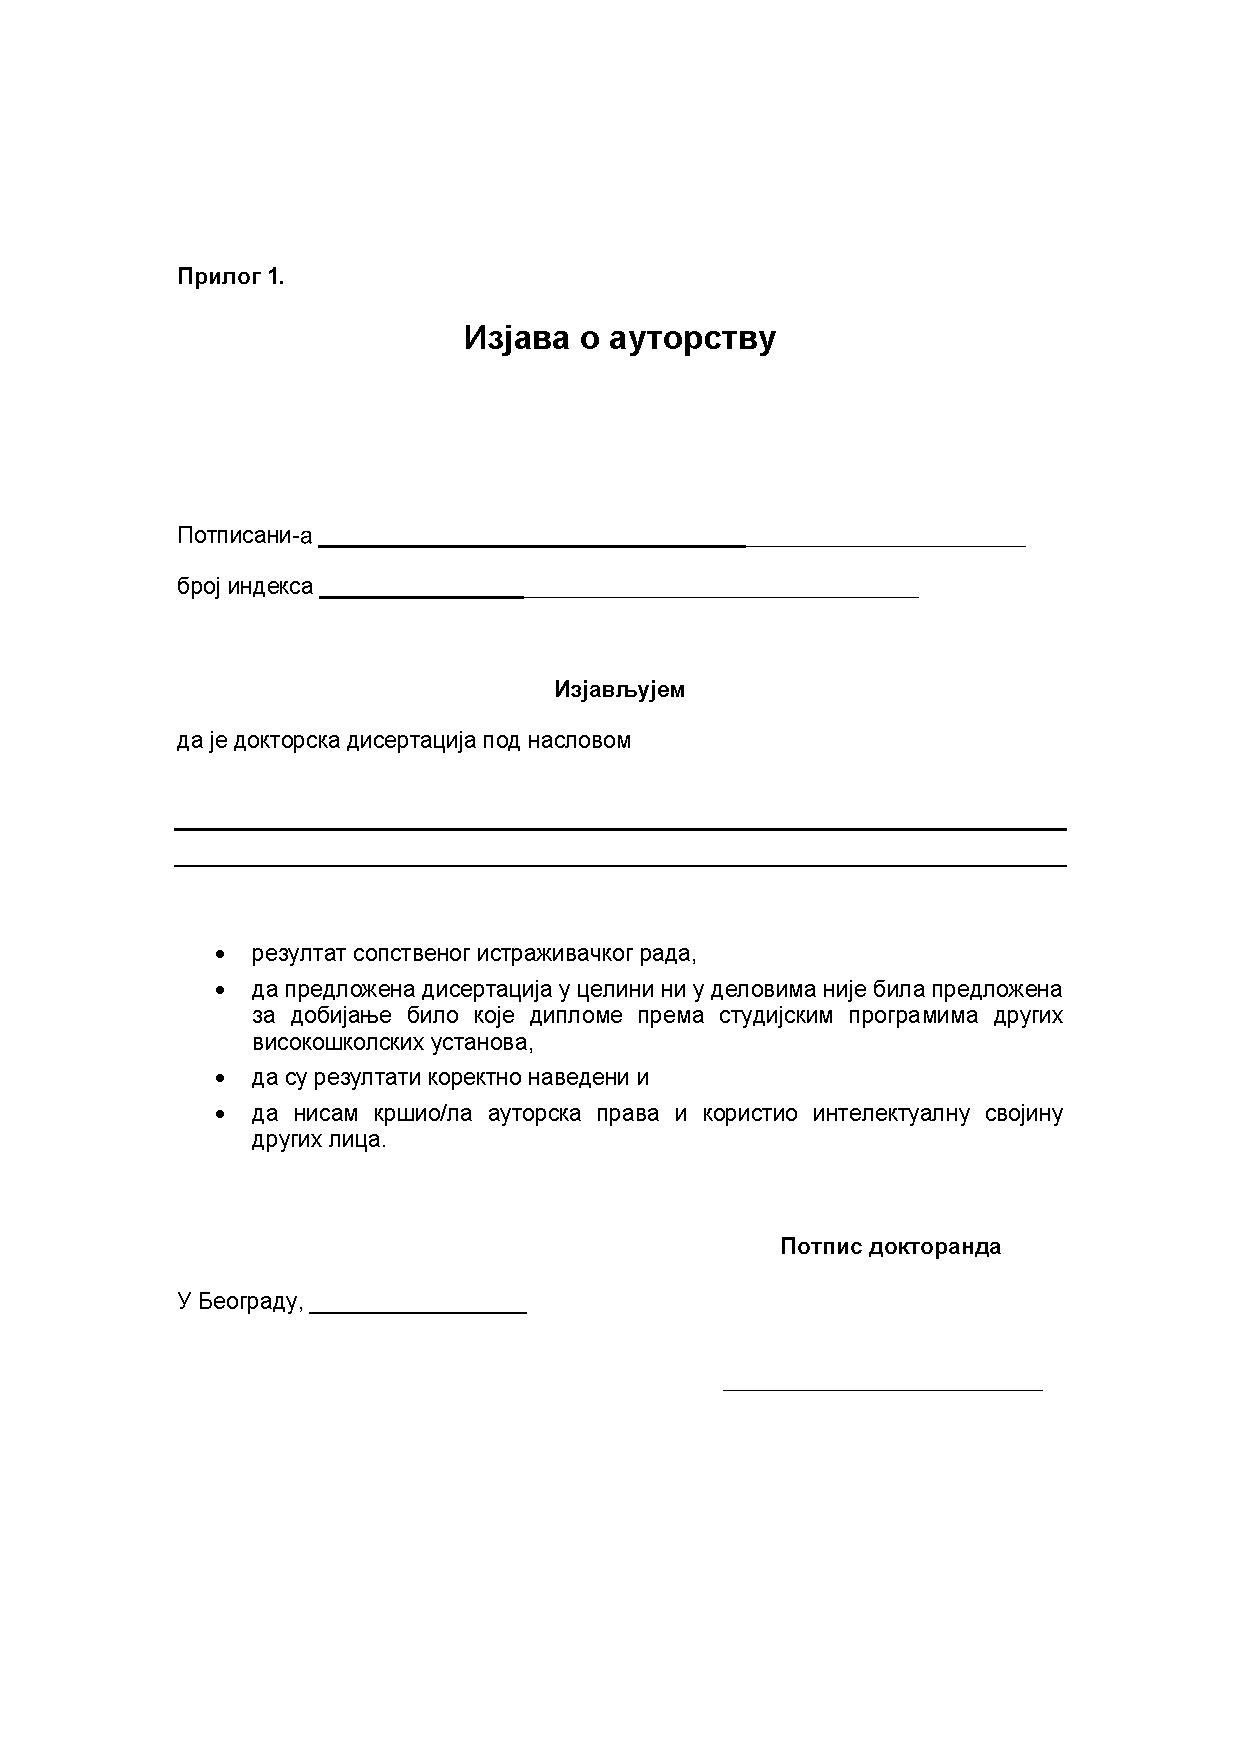
\includepdf{_Prilog1.pdf}
% Prilog 2: Izjava o istovetnosti štampane i elektronske verzije doktorskog rada
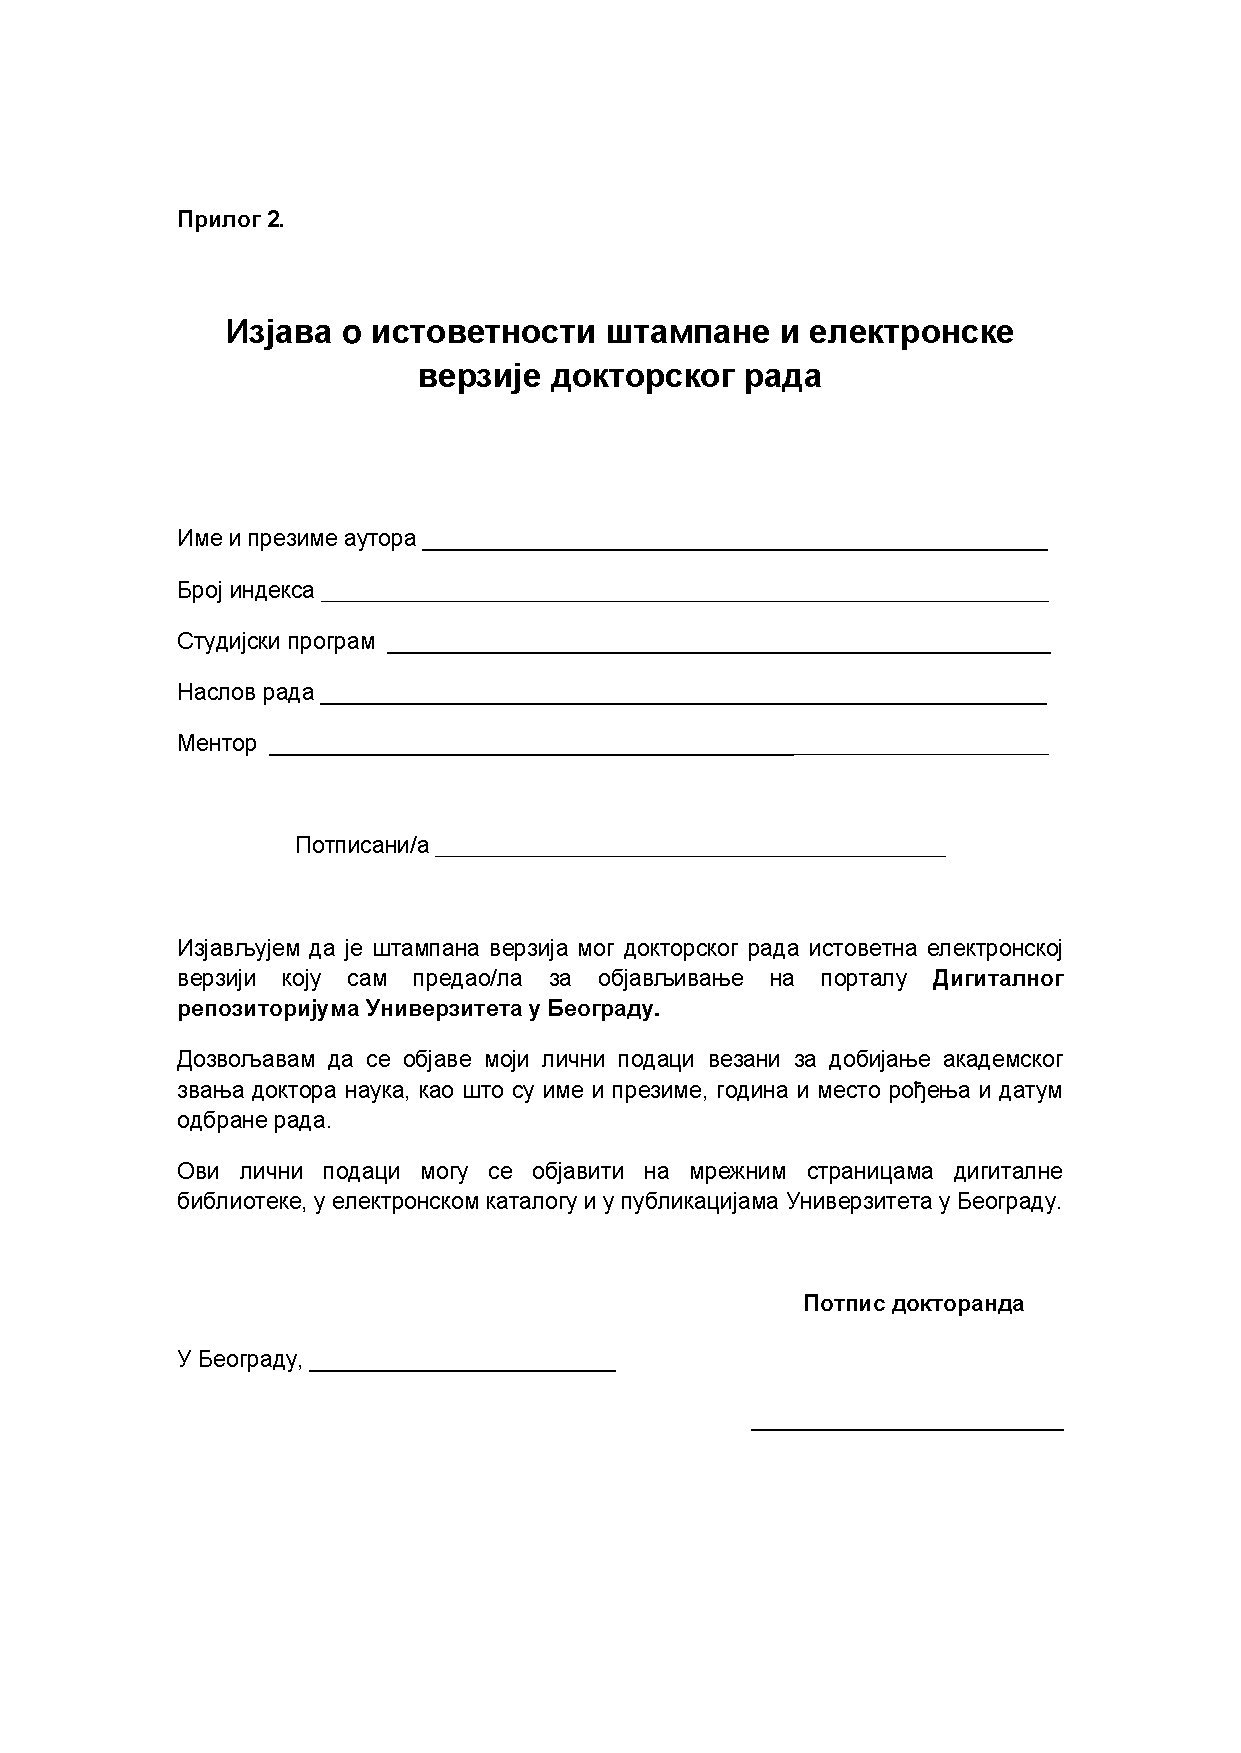
\includepdf{_Prilog2.pdf}
% Prilog 3: Izjava o korišćenju
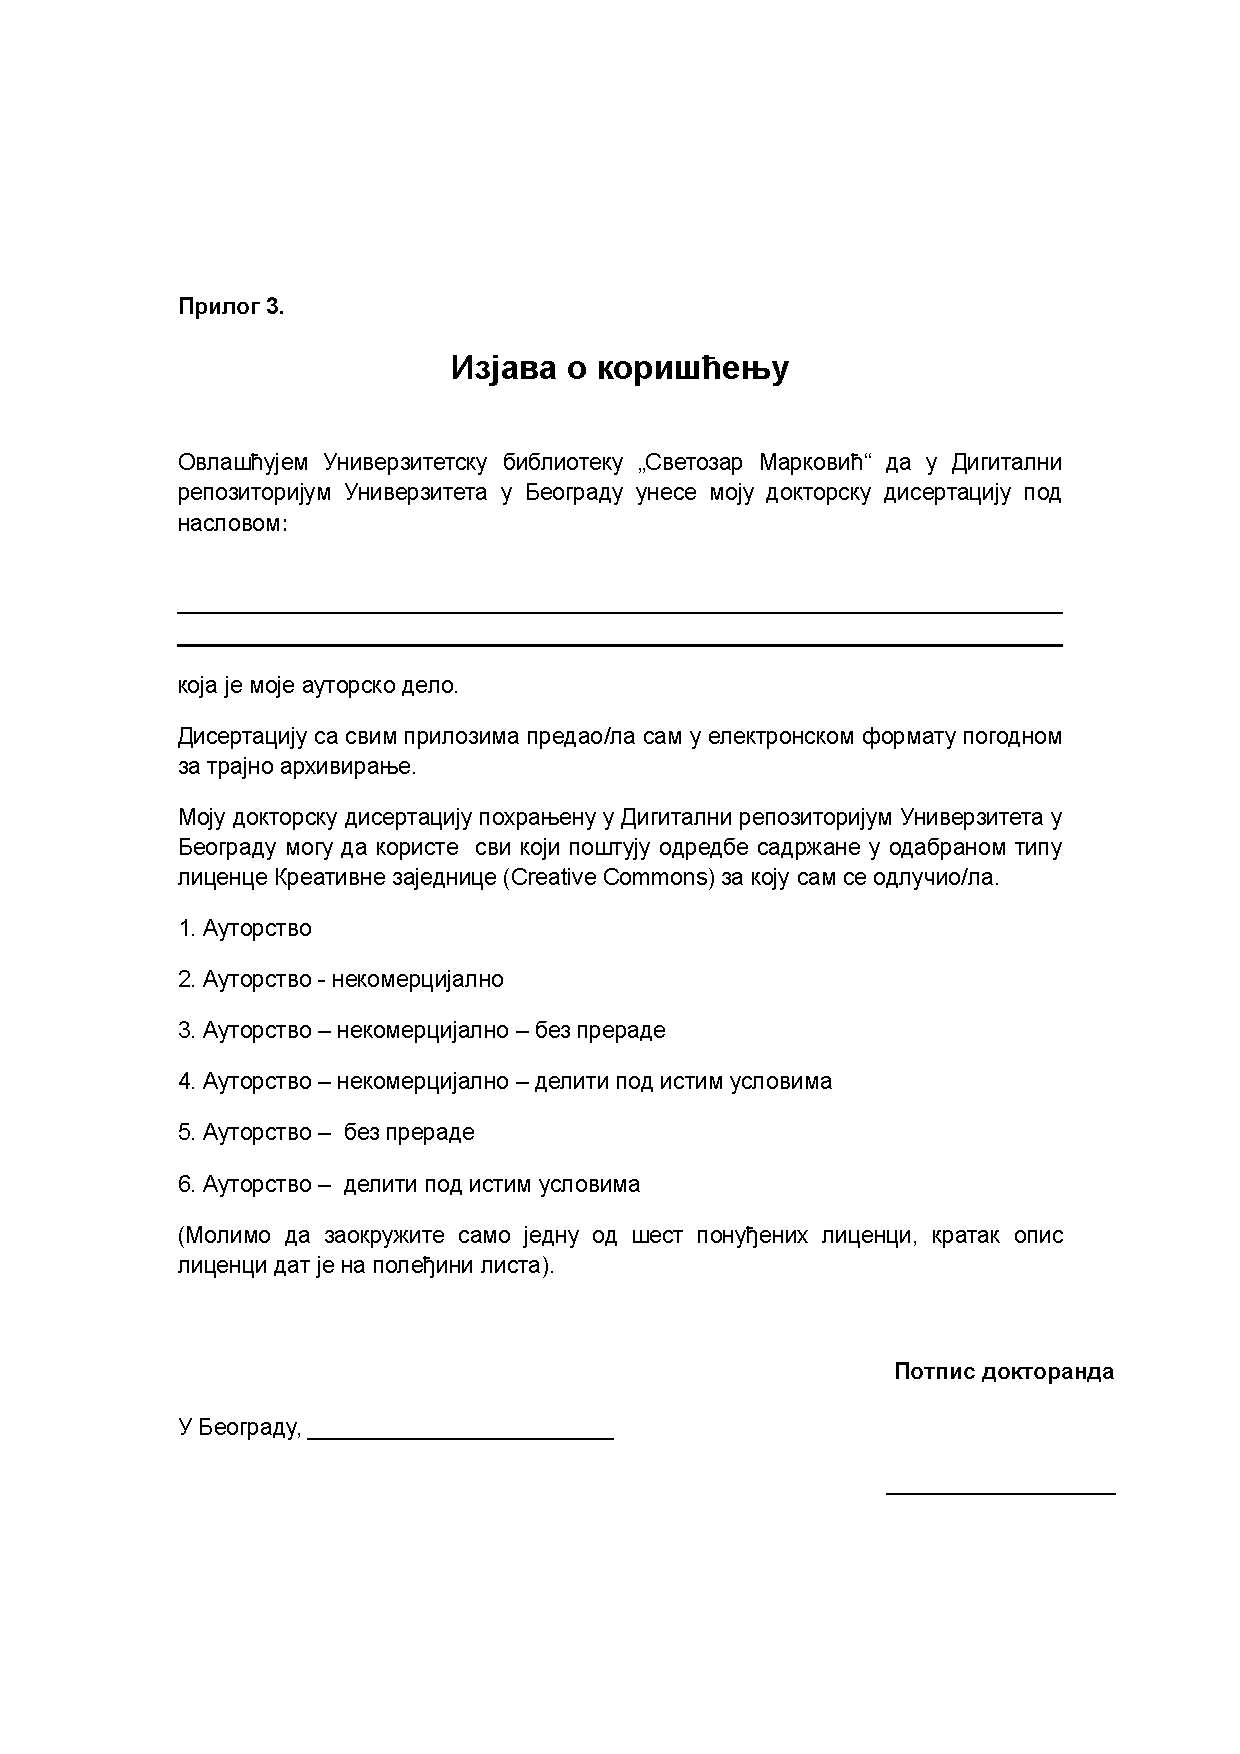
\includepdf{_Prilog3.pdf}

\end{document} 


